\documentclass[10pt,a4paper]{elsarticle}
\usepackage[utf8]{inputenc}
\usepackage[T1]{fontenc}
%\usepackage[spanish]{babel}
\usepackage{amsmath}
\usepackage{amsfonts}
\usepackage{amssymb}
\usepackage{graphicx}
\usepackage{mathtools,amssymb}
%\usepackage{subfigure}
%\usepackage{subfig}
\usepackage{caption}
\usepackage{subcaption}
\usepackage{booktabs}
\usepackage{optidef}
\usepackage{amsthm}
\usepackage{comment}
\usepackage{pgfplots}
\usepackage{soul}
\usepackage{mathrsfs}
\usepackage[ruled]{algorithm2e}
\usepackage{xspace}
\usepackage{ulem}
\usepackage{multirow}
\usepackage{bigstrut}
% \usepackage{booktabs}
\usepackage{url}

\usepackage{algorithm}
\usepackage{algpseudocode}
\newtheorem*{remark}{Remark}
\newtheorem{theorem}{Theorem}[section]
\newtheorem{corollary}{Corollary}[theorem]
\newtheorem{lemma}[theorem]{Lemma}
\allowdisplaybreaks

\usepackage[margin=1in]{geometry}

\def\MDR{{\sf MDRPG\xspace}}
\def\AMD{{\sf AMMDRPG\xspace}}
\def\AMDCO{{\sf AMMDRPG-CO\xspace}}
\def\AMDPO{{\sf AMMDRPG-PO\xspace}}
\def\NMD{{\sf NMDRPG\xspace}}
\def\PMD{{\sf PMDRPG\xspace}}
\definecolor{armygreen}{rgb}{0.19, 0.53, 0.43}
\definecolor{atomictangerine}{rgb}{1.0, 0.6, 0.4}
% \newcommand{\JP}[1]{{\color{armygreen}#1}}
% \newcommand{\CV}[1]{{\color{atomictangerine}#1}}
% \newcommand{\LA}[1]{{\color{red}#1}}
% \newcommand{\RE}[1]{{\color{blue}#1}}
\newcommand{\JP}[1]{{\color{black}#1}}
\newcommand{\CV}[1]{{\color{black}#1}}
\newcommand{\LA}[1]{{\color{black}#1}}
\newcommand{\RE}[1]{{\color{black}#1}}
\renewcommand{\arraystretch}{1.5}



\title{Coordinating drones with mothership vehicles: The mothership and multiple drones routing problem with Graphs}

\author[1]{Lavinia Amorosi\corref{cor1}}
\ead{lavinia.amorosi@uniroma1.it}
\author[2]{Justo Puerto\corref{cor1}}
\ead{puerto@us.es}
\author[2]{Carlos Valverde\corref{cor1}}
\ead{cvalverde@us.es}

\cortext[cor1]{Equally contributing authors}

\address[1]{Department of Statistical Sciences, Sapienza University of Rome, Italy}
\address[2]{Department of Statistical Sciences and Operational Research, University of Seville, Spain}



%\author{Lavinia Amorosi^{a}, Justo Puerto^{b}, Carlos Valverde^{b}}
%\address[1]{Department of Statistical Sciences, University of Rome, Sapienza}
%\address[2]{IMUS, Mathematical Research Institute, University of Seville}

\date{\today}

\begin{document}


\begin{abstract}
This paper considers the optimization problems that arise to coordinate a tandem between a mothership vehicle and a fleet of drones. %more than one drone. 
Each drone can be launched from the mothership to perform a task. After completing the tasks\RE{,} the drones return to the mothership to recharge \RE{the} batteries and to be ready for a new task. Tasks consist on (partially) visiting graphs with \RE{a given length} to deliver some services or to perform some surveillance/inspection activity.  The goal is to minimize the overall \RE{time of travelling made} by the mothership while satisfying some requirements in terms of fractions of visits to the target graphs. In all cases, we develop exact formulations resorting to mixed integer second\CV{-}order cone programs that are compared on a testbed of instances to assess their performance. We also develop a matheuristic algorithm that provides reasonable solutions.  Computational experiments show the usefulness of our \RE{methodology} in different scenarios.  %\CV{We haven't mentioned both variants of the problem and we are using operation (maybe change it by task)?}
\end{abstract}

\begin{keyword}
Arc Routing Problems \sep Networks \sep Drones \sep Conic Programming
\end{keyword}


\maketitle


%\section{Introduction}
In recent years the grow of the potential business opportunities related to the use of drone technology has motivated the appearance of an interesting body of methodological literature on optimizing of the use of such technology. 
We can find examples of that in many different sectors, like telecommunication where drones can be adopted in place of traditional infrastructures to provide connectivity (see for example \cite{art:Amorosi2018}, \cite{art:Chiaraviglio2018}, \cite{Jimenez2018}, \cite{art:Amorosi2019}, and \cite{art:Chiaraviglio2019a}), or to temporary deal with the damages caused by a disaster (\cite{art:Chiaraviglio2019}), deliveries (see for example \cite{art:Mathew2015} , \cite{art:Ferrandez2016}, \cite{art:Poikonen2020} and \cite{art:Amorosi2020}), also in emergency contexts (\cite{art:Wen2016}), inspection (\cite{art:Trotta2018}) and others.
The reader is referred to the recent surveys \cite{art:Otto2018} and \cite{art:Chung2020} for further details.\\
\noindent
Among the different aspects that can be considered we want to focus, for its relationship to the development in this paper, to the design, coordination and optimization of the combined routes of drones with a base vehicle. After the initial paper \cite{MURRAY201586} by Murray and Chu, where a combined model of truck and drone is considered, the work of Ulmer and Thomas \cite{Ulmer2018} also considers another model where trucks and drones are dispatched as order are placed and analyze the effect of different policies for either the truck or the drone. Other papers, as for instance, \cite{art:Campbell2017}, \cite{art:Carlsson2017} and \cite{art:Dayarian2017}, have also considered hybrid truck-and-drone models in order to mitigate the limited delivery range of drones. Poikonen and Golden, in \cite{Poikonen2019}, advance on the coordination problem considering the \textit{Mothership and drone routing problem} where these two vehicles are used to design a route that visits a number of points allowing the truck to launch and recover the drone in a continuous space. More recently in \cite{art:Poikonen2020} the authors consider the \textit{$k$-Multi-Visit drone routing problem} where a truck that acts as a mobile depot only allowed to stop in a predefined set of points, launches drones that can deliver more than one package to their designated destination points.
\noindent
Many of these papers make the assumptions that the set of allowable locations to launch/retrieve a drone are fixed and known a priori, the operations performed by the drone consist of delivering to a single point and the coordination is between a truck and a single drone. These assumptions may be appropriate in some frameworks but in other cases it may be better to relax them.\\
\noindent
In particular, only few papers in literature focus on drones operations consisting in traversing graphs rather than visiting single points. Campbell et al. 
\cite{art:Campbell2018} introduce the \textit{Drone Rural Postman Problem} (DRPP). The authors present a solution algorithm based on the approximation of curves in the plane by polygonal chains and that iteratively increases the number of points in the polygonal chain where the UAV can enter or leave. Thus, they solve the problem as a discrete optimization problem trying to better define the curve by increasing the number of points. The authors consider also the case in which the drone has limited capacity and thus it cannot serve all the lines. To deal with this latter case, they assume to have a fleet of drones and the problem consists in finding a set of routes, each of limited length.\\
In \cite{art:CAMPBELL202160}  this problem has been defined as the \textit{Length Constrained K-drones Rural Postman Problem}, a continuous optimization problem where a fleet of homogeneous drones have to jointly service (traverse) a set of (curved or straight) lines of a network. The authors design and implement a branch-and-cut algorithm for its solution and a matheuristic algorithm capable of providing good solutions for large scale instances of the problem.\\
Scanning the literature of arc routing problems involving hybrid systems consisting in one vehicle and one or multiple drones, the number of contributions is rather limited.\\
In \cite{art:Tokekar2016} the authors study the path planning problem of a system composed of a ground robot and one drone in precision agriculture and solve it by applying orienteering algorithms. Also the paper \cite{art:Garone2010} studies the problem of paths planning for systems consisting in a carrier vehicle and a carried one to visit a set of target points and assuming that the carrier vehicle moves in the continuous space.\\
To the best of our knowledge, only the paper \cite{art:Amorosi2021}, deals with the coordination of a mothership with one drone to visit targets represented by graphs. The authors made different assumptions on the route followed by the mothership: it can move on a continuous framework (the Euclidean plane), ii) on a connected piecewise linear polygonal chain or iii) on a general graph. In all cases, the authors develop exact formulations resorting to mixed integer second order cone programs and propose a matheuristic algorithm capable to obtain high quality solutions in short computing time.
\\
In this paper we deal with an extension of the problem studied in \cite{art:Amorosi2021} for which we propose a novel truck-and-multi-drones coordination model. We consider a system where a base vehicle (mothership) can stop anywhere in a continuous space and has to support the launch/retrieve of a number of drones that must visit graphs. The contribution on the existing literature is to extend the coordination beyond a single drone to the more cumbersome case of several drones and the operations to traversing graphs rather than visiting single points. In particular, we focus on a synchronous version in which every drone is launched and retrieved in the same stage. We present a mathematical programming formulation, valid inequalities to reinforce it and a matheuristic to deal with large instances of this problem. Moreover, we discuss and show how to extend further the former case to the  asynchronous situation where one assumes that the mothership can retrieve one drone in a different stage from the one in which it has been launched.\\
\noindent
The work is structured as follows: Section 2 provides a detailed description of the problem under consideration and develops a valid mixed integer non linear programming formulations for it. Section 3  provides some valid inequalities that strengthen the formulation and also derives upper and lower bounds on the big-M constants introduced in the proposed formulation. Section 4 presents details of the matheuristic algorithm designed to handle large instances. In Section 5 we report the results obtained testing the formulation and the matheuristic algorithm on different classes of planar graphs in order to assess its effectiveness. Finally, Section 6 concludes the paper.
\section{Introduction}
\noindent
In recent years\RE{,} the grow of \RE{potential} business opportunities related to the use of drone technology \RE{have} motivated the appearance of an interesting body of methodological literature on \RE{the optimization} of the use of such technology. 
We can find examples of that in many different sectors, like telecommunication\RE{s} where drones can be adopted in place of traditional infrastructures to provide connectivity (see\RE{,} for example \cite{art:Amorosi2018}, \cite{art:Chiaraviglio2018}, \cite{Jimenez2018}, \cite{art:Amorosi2019}, and \cite{art:Chiaraviglio2019a}), or to temporary deal with the \RE{damage} caused by a disaster (\cite{art:Chiaraviglio2019}), deliveries (see\RE{,} for example \cite{art:Mathew2015} , \cite{art:Ferrandez2016}, \cite{art:Poikonen2020} and \cite{art:Amorosi2020}), also in emergency contexts (\cite{art:Wen2016}), inspection (\cite{art:Trotta2018}) and others.
The reader is referred to the recent surveys \cite{art:Otto2018} and \cite{art:Chung2020} for further details.\\
\noindent
Among the different aspects that can be considered\RE{,} we want to focus, \RE{due to} its relationship to the development in this paper, to the design, coordination and optimization of the combined routes of drones with a base vehicle. After the initial paper \cite{MURRAY201586}, where a combined model of truck and drone is considered, the work \cite{Ulmer2018} also considers another model where trucks and drones are dispatched as \RE{the} order\RE{s} are placed and analyze the effect of different policies for either the truck or the drone. Other papers, as\RE{,} for instance, \cite{art:Campbell2017}, \cite{art:Carlsson2017} and \cite{art:Dayarian2017}, have also considered hybrid truck-and-drone models in order to mitigate the limited delivery range of drones. In \cite{Poikonen2019} the authors advance on the coordination problem considering the \textit{Mothership and drone routing problem} where these two vehicles are used to design a route that visits a number of points allowing the truck to launch and recover the drone in a continuous space. More recently, in \cite{art:Poikonen2020}, the authors consider the \textit{$k$-Multi-Visit drone routing problem} where a truck that acts as a mobile depot only allowed to stop in a predefined set of points, launches drones that can deliver more than one package to their designated destination points. %\CV{There are some references where we mention the authors, and other not}
\noindent
Many of these papers make \RE{assumptions} that the set of allowable locations to launch/retrieve a drone are fixed and known a priori, the \CV{operations} performed by the drone consist of delivering to a single point and the coordination is between a truck and a single drone. These assumptions may be appropriate in some frameworks\RE{,} but, in other cases, it may be better to relax them.\\
\noindent
In particular, only \RE{a} few papers in \RE{the} literature focus on \RE{drone} operations consisting \RE{of} traversing graphs rather than visiting single points. Later authors in 
\cite{art:Campbell2018} introduce the \textit{Drone Rural Postman Problem} (DRPP). \RE{Those} authors present a solution algorithm based on the approximation of curves in the plane by polygonal chains \CV{that iteratively} increases the number of points in the polygonal chain where the UAV can enter or leave. Thus, they solve the problem as a discrete optimization problem trying to better define the curve by increasing the number of points. The authors consider also the case in which the drone has limited \RE{endurance} and thus it cannot serve all the lines. To deal with this latter case, they assume to have a fleet of drones and the problem consists in finding a set of routes, each of limited length.\\
In \cite{art:CAMPBELL202160}  this problem has been defined as the \textit{Length Constrained K-drones Rural Postman Problem}, a continuous optimization problem where a fleet of homogeneous drones have to jointly service (traverse) a set of (curved or straight) lines of a network. The authors design and implement a branch-and-cut algorithm for its solution and a matheuristic algorithm capable of providing good solutions for large\RE{-}scale instances of the problem.\\
Scanning the literature of arc routing problems involving hybrid systems consisting \RE{of} one vehicle and one or multiple drones, the number of contributions is rather limited.\\
In \cite{art:Tokekar2016} the authors study the path planning problem of a system composed of a ground robot and one drone in precision agriculture and solve it by applying orienteering algorithms. \RE{Moreover,} the paper \cite{art:Garone2010} studies the problem of \RE{path} planning for systems consisting \RE{of} a carrier vehicle and a carried one to visit a set of target points and assuming that the carrier vehicle moves in the continuous space.\\
To the best of our knowledge, \RE{the paper \cite{art:Amorosi2021} is the only one} that deals with the coordination of a mothership with one drone to visit targets represented by graphs. The authors made different assumptions on the route followed by the mothership: it can move on a continuous framework (the Euclidean plane), ii) on a connected piecewise linear polygonal chain\RE{,} or iii) on a general graph. In all cases, the authors develop exact formulations resorting to mixed integer second\RE{-}order cone programs and propose a matheuristic algorithm capable to obtain high quality solutions in short computing time.
\\
In this paper we deal with an extension of the problem studied in \cite{art:Amorosi2021} for which we propose a novel truck-and-multi-\RE{drone} coordination model. We consider a system where a base vehicle (mothership) \RE{travels} in \JP{the} continuous space and has to support the launch/retrieve of a number of drones that must visit graphs. \RE{Our} contribution \RE{over} the existing literature is to extend the coordination beyond a single drone to the more cumbersome case of several drones and operations to traversing graphs rather than visiting single points. 
\noindent
\JP{In particular, we focus on two different versions. In the first one, called \textit{complete overlapping model}, operations consisting on the launching and retrieving of a set of drones are done sequentially so that no two consecutive launching are  possible without retrieving the previously launched drones (See Figure \ref{fig:2-models} left).  The second version, called \textit{partial overlapping model}, allows consecutive launching or retrieving actions so that the visits of several drones to their target graphs are allowed to partially overlap over the time (See Figure \ref{fig:2-models} right). In both cases, we present  mathematical programming formulations, valid inequalities to strengthen them and ad hoc matheuristics to deal with large sized instances of the problem.\\}
\noindent

%% \pgfplotsset{compat=1.15}
\usetikzlibrary{arrows}
\begin{figure}[h!]
\centering
\definecolor{ffwwzz}{rgb}{1,0.4,0.6}
\definecolor{ffqqqq}{rgb}{1,0,0}
\begin{tikzpicture}[line cap=round,line join=round,>=triangle 45,x=0.5cm,y=0.5cm]
\fill[line width=2pt,fill=black] (3.8,5.2) -- (4.2,5.2) -- (4.2,4.8) -- (3.8,4.8) -- cycle;
\fill[line width=2pt,fill=black] (15.8,5.2) -- (16.2,5.2) -- (16.2,4.8) -- (15.8,4.8) -- cycle;
\fill[line width=2pt,fill=black] (18.8,5.2) -- (19.2,5.2) -- (19.2,4.8) -- (18.8,4.8) -- cycle;
\fill[line width=2pt,fill=black] (30.8,5.2) -- (31.2,5.2) -- (31.2,4.8) -- (30.8,4.8) -- cycle;
\draw [line width=3.5pt] (4,5)-- (7,5);
\begin{scope}[transparency group, opacity=0.5]
\draw [-stealth,line width=3.5pt,color=ffqqqq] (7,5) -- (9,8);
\draw [-stealth,line width=3.5pt,color=ffqqqq] (7,5) -- (11,1.974194108172913);
\draw [-stealth,line width=3.5pt,color=ffqqqq] (9,8) -- (13,4.974194108172913);
\draw [-stealth,line width=3.5pt,color=ffqqqq] (11,1.974194108172913) -- (13,4.974194108172913);
\end{scope}
\draw [line width=3.5pt,color=ffqqqq] (7,5)-- (13,4.974194108172913);
\draw [line width=3.5pt] (13,4.974194108172913)-- (16,5);
\draw [line width=3.5pt] (19,5)-- (22,5);
\draw [line width=3.5pt] (28,5)-- (31,5);
\begin{scope}[transparency group, opacity=0.5]
\draw[-stealth,line width=3.5pt, red] (22,5) -- (24,8);
\draw[-stealth,line width=3.5pt, red] (24,8) -- (26,5);
\draw[-stealth,line width=3.5pt, red] (24,5) -- (26,2);
\draw[-stealth,line width=3.5pt, red] (26,2) -- (28,5);
\end{scope}
\draw [line width=3.5pt,color=ffqqqq] (24,5)-- (26,5);
\draw [line width=3.5pt,color=ffqqqq, opacity=0.5] (22,5)-- (24,5);
\draw [line width=3.5pt,color=ffqqqq, opacity=0.5] (26,5)-- (28,5);
\begin{scriptsize}
\draw [fill=ffqqqq] (7,5) circle (2.5pt);
\draw [fill=ffwwzz] (9,8) circle (2.5pt);
\draw [fill=ffwwzz] (11,1.974194108172913) circle (2.5pt);
\draw [fill=ffqqqq] (13,4.974194108172913) circle (2.5pt);
\draw [fill=ffwwzz] (22,5) circle (2.5pt);
\draw [fill=ffqqqq] (28,5) circle (2.5pt);
\draw [fill=ffwwzz] (24,8) circle (2.5pt);
\draw [fill=ffwwzz] (26,2) circle (2.5pt);
\draw [fill=ffwwzz] (26,5) circle (2.5pt);
\draw [fill=ffwwzz] (24,5) circle (2.5pt);
\end{scriptsize}
\end{tikzpicture}
\caption{Models with complete and partial overlapping.\label{fig:2-models}}
\end{figure}
% \pgfplotsset{compat=1.15}
\usetikzlibrary{arrows}
\begin{figure}[h!]
\centering
%\definecolor{ffwwzz}{rgb}{1,0.4,0.6}
%\definecolor{gray}{rgb}{1,0,0}
\begin{tikzpicture}[line cap=round,line join=round,>=triangle 45,x=0.5cm,y=0.5cm]
\fill[line width=2pt,fill=black] (3.8,5.2) -- (4.2,5.2) -- (4.2,4.8) -- (3.8,4.8) -- cycle;
\fill[line width=2pt,fill=black] (15.8,5.2) -- (16.2,5.2) -- (16.2,4.8) -- (15.8,4.8) -- cycle;
\fill[line width=2pt,fill=black] (18.8,5.2) -- (19.2,5.2) -- (19.2,4.8) -- (18.8,4.8) -- cycle;
\fill[line width=2pt,fill=black] (30.8,5.2) -- (31.2,5.2) -- (31.2,4.8) -- (30.8,4.8) -- cycle;
\draw [line width=3.5pt] (4,5)-- (7,5);
\begin{scope}[transparency group, opacity=0.5]
\draw [-stealth,line width=3.5pt,color=gray] (7,5) -- (9,8);
\draw [-stealth,line width=3.5pt,color=gray] (7,5) -- (11,1.974194108172913);
\draw [-stealth,line width=3.5pt,color=gray] (9,8) -- (13,4.974194108172913);
\draw [-stealth,line width=3.5pt,color=gray] (11,1.974194108172913) -- (13,4.974194108172913);
\end{scope}
\draw [line width=3.5pt,color=gray] (7,5)-- (13,4.974194108172913);
\draw [line width=3.5pt] (13,4.974194108172913)-- (16,5);
\draw [line width=3.5pt] (19,5)-- (22,5);
\draw [line width=3.5pt] (28,5)-- (31,5);
\begin{scope}[transparency group, opacity=1]
\draw[-stealth,line width=3.5pt, lightgray] (22,5) -- (24,8);
\draw[-stealth,line width=3.5pt, lightgray] (24,8) -- (26,5);
\draw[-stealth,line width=3.5pt, lightgray] (24,5) -- (26,2);
\draw[-stealth,line width=3.5pt, lightgray] (26,2) -- (28,5);
\end{scope}
\draw [line width=3.5pt,color=gray] (24,5)-- (26,5);
\draw [line width=3.5pt,color=gray, opacity=0.5] (22,5)-- (24,5);
\draw [line width=3.5pt,color=gray, opacity=0.5] (26,5)-- (28,5);
\begin{scriptsize}
\draw [fill=gray] (7,5) circle (2.5pt);
\draw [fill=lightgray] (9,8) circle (2.5pt);
\draw [fill=lightgray] (11,1.974194108172913) circle (2.5pt);
\draw [fill=gray] (13,4.974194108172913) circle (2.5pt);
\draw [fill=lightgray] (22,5) circle (2.5pt);
\draw [fill=gray] (28,5) circle (2.5pt);
\draw [fill=lightgray] (24,8) circle (2.5pt);
\draw [fill=lightgray] (26,2) circle (2.5pt);
\draw [fill=lightgray] (26,5) circle (2.5pt);
\draw [fill=lightgray] (24,5) circle (2.5pt);
\end{scriptsize}
\end{tikzpicture}
\caption{Models with complete and partial overlapping.\label{fig:2-models}}
\end{figure}

\noindent
\JP{The work is structured as follows: Section \ref{section:desc} provides a detailed description of the problem under consideration. Section \ref{Form}  develops valid mixed integer nonlinear programming formulations for the two versions of the considered problem. Here, we also show the relationship between the two models and prove that the second model is a relaxation of the first one. Section \ref{bounds} provides some valid inequalities that strengthen the formulations and derives upper and lower bounds on the bigM constants introduced in the proposed formulations. Section \ref{Math} presents details of the matheuristic algorithms designed to handle large sized instances. In Section \ref{section:results} we report the results obtained testing the formulations and the matheuristic algorithm on different classes of planar graphs to assess its effectiveness. In Section \ref{section:CS}, we introduce an illustrative example applying the coordination models to the Courtyards Festival of Cordoba. Section \ref{section:CR} concludes the paper. Finally, for the sake of completeness, we have included an appendix with an extension of the model of complete overlapping where the drones are not assumed to be homogeneous. %\CV{We present a mixed integer second order cone programming formulation, develop several valid inequalities to strengthen it and report computational results assessing its performance.} 
}
%\section{State of the art}
In this section we focus mainly on the previous works in literature related to systems where UAVs are assisted by a vehicle in order to serve a set of targets.
In these configurations the vehicle represents a launch and a recharging station for the UAVs and the main problem consists in coordinating the operations performed by one or multiple drones and the mothership.
Most of the previous works in literature on this subject are focused on node routing problems (NRPs), where the vehicle moves on a road network and the drone is used to visit target points outside the road network. 
Many of them are related to applications in the delivery sector where the set of targets to be visited is represented by a set of customers.
For example, \cite{art:Mathew2015} studies a delivery system consisting in one drone and one truck. The UAV visits one customer for each trip and the truck can wait at the launching node for the drone to come back or move to a different rendezvous node. In \cite{art:Carlsson2018} the authors study a continuous approximation on the Horse Fly Problem, where the truck is used as a mobile depot for the drone. In \cite{art:Campbell2017} the authors evaluate the economic impact of truck-and-drone hybrid models for deliveries by means of a continuous approximation model, considering different model parameters and customer densities. \cite{art:Ferrandez2016} focuses on a delivery system where one truck supports the operations of multiple drones. The authors first clusterize the customer demand by adopting a K-means algorithm to find truck stops that represent hubs for drone deliveries. Then, they determine a TSP of the truck among centroids of these clusters, by means of a genetic algorithm, assuming that drones are not constrained by flight range. In \cite{art:Moshref2017} the authors consider a similar delivery system where at each stop site the truck waits until all drones come back before moving to the next site. The goal is the minimization of the latency in a customer-oriented distribution system. Moreover, the authors compare the benefits of using drones for a single trip versus multiple trips. In \cite{art:Poikonen2020} the authors formalize the k-Multi-visit Drone Routing Problem (k-MVDRP) considering a tandem between a truck and a fleet of k drones. The authors assumed that each drone can deliver one or more packages to customers in a single mission. Each drone may return to the truck to swap/recharge batteries, pick up a new set of packages, and launch again to customer locations. Moreover, the authors decouple the set of launch locations from the set of customer locations. The article presents a mathematical formulation including a drone energy drain function that takes into account each package weight, but the problem is then solved by means of a heuristic algorithm.
\cite{art:Amorosi2020} presents a multi-objective mixed integer linear programming model for the management of a hybrid delivery system consisting in one base vehicle and a fleet of drones. As in \cite{art:Poikonen2020}, the set of launch locations is assumed to be different from the set of customer locations. The problem consists in determining the tour of the base vehicle and the assignments of the customers to the UAVs simultaneously optimizing the distance travelled by the vehicle, the one travelled by the drones and the maximum completion time. The model is solved on two realistic urban scenarios providing a partial exploration of the Pareto frontier of the problem by means of the weighted sum method.\\
Other examples of similar configurations in which a base vehicle supports the operations of one or multiple drones can be found also in other sectors. 
\cite{art:Trotta2018} studies, for example, the city-scale video monitoring of a set of points of interest performed by a fleet of UAVs whose operations are supported by buses and the problem is modeled as a mixed integer linear programming model based on a multi-period directed graph.
However, in all the works mentioned so far, the combined operations of vehicles and drones examine routing for a set of locations and these configurations exploit only part of the advantages of the adoption of drones. Indeed, UAVs can move between any two points in the space not following the road network. Thus, they can be adopted also for other kind of services in which the targets are represented by edges or part of them. This leads to another class of models, that is arc routing problems (ARPs).\\
With respected to NRPs, in the case of ARPs with drones there are relatively few papers. \cite{art:Oh2011} and \cite{art:Oh2014} study a coordinated road network search problem with multiple UAVs and they formulated it as a Multi-choice Multi-dimensional Knapsack Problem minimizing the flight time. This is a modified Chinese Postman Problem taking into account the UAVs energy \RE{\sout{endurance} endurance} constraints. The authors solved the problem by means of a greedy insertion heuristic that models drone travel distance between the road components as a Dubins path.
\cite{art:Dille2013} faces the area coverage problem in sparse environments with multiple UAVs. Also in this case the UAVs motion is modeled using Dubins paths and it is assumed that they are equipped with a coverage sensor of a given radius.
The edge covering problem is solved by discretizing the network in orbits and then solving a TSP among this set of orbits. The authors compares the results obtained with the ones obtained with the method by \cite{art:Oh2014}, for simulated urban, suburban and rural scenarios, showing that for suburban densities their method outperforms both with one or multiple UAVs. 
In \cite{art:Chow2016} the authors deal with the problem of dynamically allocate a finite set of UAVs to links in a network that need monitoring, over multiple time periods. The need of drone monitoring is based on data related to traffic conditions. They formulated the first deterministic multi-period arc-inventory routing problem and then its stochastic dynamic version solved with an approximate dynamic programming algorithm. 
Another work related to multiple-period real-time monitoring of road traffic, adopting UAVs, is \cite{art:Li2018}. The authors proposed a mixed integer programming model combining the capacitated arc routing problem with the inventory routing problem and designed a local branching based method for dealing with large instances.\\
The ARPs with one UAV, have common characteristics with problems arising in path generation for laser cutting machines or drawing plotters. In particular, the authors of \cite{art:Campbell2018} studied the Drone Rural Postman Problem (DRPP) showing the relation with the Intermittent Cutting Problem (ICP). They presented a solution algorithm based on the approximation of curves in the plane by polygonal chains and that iteratively increases the number of points in the polygonal chain where the UAV can enter or leave. Thus, they solved the problem as a discrete optimization problem trying to better define the line by increasing the number of points. The authors considered also the case in which the drone has limited \RE{\sout{endurance} endurance} and thus it cannot serve all the lines. To deal with this latter case, the authors assumed to have a fleet of drones and the problem consisted in finding a set of routes, each of limited length.\\
The literature related to Drone ARPs is limited with respect to the one related to Drone NRPs.
However, as regards arc routing problems involving a hybrid system consisting in one vehicle and one or multiple drones, the number of contributions in literature is further restricted and we can just mention \cite{art:Tokekar2016} and \cite{art:Garone2010}.\\
In \cite{art:Tokekar2016} the authors studied the path planning problem of a system composed of a ground robot and one drone in precision agriculture and solved it by applying orienteering algorithms. \cite{art:Garone2010} studied the problem of paths planning for systems consisting in a carrier vehicle and a carried one to visit a set of target points and assuming that the carrier vehicle moves in the continuous space. In particular, the authors formulated two different problems: the first one consisting in determining the takeoff/landings sequences of the carried vehicle to visit a set of points, assuming that in each mission of the carried vehicle only one target can be visited. The second one in which this constraint is removed permitting to the carried vehicle to visit more than one target in a single mission, before returning to the carrier vehicle. Heuristic approaches have been proposed to deal with both problems.\\
To the best of our knowledge none of the previous papers in literature deals with a drone arc routing problem combined with a node routing problem for a hybrid system consisting of one vehicle and one drone.
In this paper we present new Mixed Integer Non-Linear Programming (MINLP) formulations for the problem of coordinating a system composed of a mothership (the base vehicle) which supports the operations of one drone which has to visit a set of targets represented by graphs, with the goal of minimizing the total distance travelled by both vehicles.
Indeed, differently from the previous works in literature, we assume the drone can move freely on the continuous space. As regards the mothership, we studied both cases in which also the base vehicle can move freely on the continuous space or it is constrained to move on a road network, of different typologies, where launching and rendezvous points can be chosen.
The main contributions of this article can be summarized as follows:
\begin{itemize}
    \item New mathematical formalization of the coordinating problem of a base vehicle and one drone in the continuous space to visit a set of targets represented by graphs;
    \item Design of new alternative second order cone MINLP formulations;
    \item A new matheuristic algorithm to deal with large instances able to provide high quality solutions in short time;
    \item Extensive experimental analysis comparing the exact solution of the formulations and the matheuristic on a set of generated instances involving different typology of planar graphs.
\end{itemize}
 


% \section{Problem description and valid formulation}\label{section:desc}
% Datos iniciales del problema

\subsection{Problem description}
In the All terrain Mothership and Multiple Drones Routing Problem with Graphs (\AMD), there is one mothership (the base vehicle) and a fleet of homogeneous drones $\mathcal D$ that have to coordinate among them and with the mothership to perform a number of operations consisting in visiting given percentages of the length of a set of graphs $\mathcal G$. The mothership and the drones travel at constant velocities $v_M$ and $v_D$, respectively. Moreover, it is assumed that each  drone has a limited flying autonomy (endurance) $N^d$, so that once it is launched it must complete the operation and return back to the base vehicle to recharge batteries before the time limit. The base vehicle can move freely on a continuous space and starts at a known location, denoted $orig$ where the mothership and the fleet of drones are ready to depart. Once all the operations are finished the mothership and the drones must return together to a final location, called $dest$. 
%Finally, the mothership is allowed to move freely in a continuous space: $\mathbb R^2$ or $\mathbb R^3$.
\noindent
The set of target graphs $\mathcal G$ to be visited  permits to model real situations like monitoring and inspection activities on portions of networks (roads or wires) where traditional vehicles cannot arrive, due to, for example,  the presence of narrow streets, or because of a natural disaster or a terrorist attack that caused damages on the network. In all these cases, the inspection or monitoring of the drone consists in traversing edges of the network to perform a reconnaissance activity. For this reason we model the targets, to be visited by the drone, as graphs. The operation of visiting a graph can be of two different types: 1) traversing a given percentage of the length of each one of its edges or 2) visiting a percentage of the total length of the network. 

% In this case, for the sake of simplicity, it is assumed that there exist no obstacles to prevent drone travelling in straight line. Nevertheless, that extension is interesting to be further considered although is beyond the scope of this paper.\\

\noindent
In this problem, it is assumed that each graph must be visited by one drone: once the drone assigned to the operation enters the graph, it has to complete the entire operation of traversing this target before to be able to leave the graph to return to the base. Moreover, at each stage the drones must be launched from the mothership at the same point (the launching points have to be determined) and they also must be retrieved at the same point (the rendezvous points also have to be determined). However, this does not mean that the mothership and all drones must arrive at a rendezvous location at the same time: the fastest arriving vehicle may wait for the others at the rendezvous location. Note also that every drone of the fleet does not have to be launched from the current base vehicle location in all the stages because of the capacity constraint. In addition, it is supposed that the cost induced by the drones' trips are negligible as compared to those incurred by the base vehicle. Therefore, the goal is to minimize the overall distance traveled by the mothership. In spite of that, the reader may note that from a theoretical point of view the extension to include in the objective function also the distances traveled by the drones is straightforward and does not increase the complexity of the models and formulations.
\noindent
The goal of the \AMD \ is to find the launching and rendezvous points of the fleet of drones $\mathcal D$ satisfying the visit requirements for the graphs in $\mathcal G$ and minimizing the length of the path traveled by the mothership.\\

\noindent



% The mothership and the drone begin at a starting location, denoted $orig$ and a set $\mathcal G$ of target locations modeled by graphs, that must be visited by the drone, are located in the plane. These assumptions permit to model several real situations like roads or wired networks inspection.
% %The natural application for this situation comes from road or wired network inspection. 
% For each stage $t \in \{1, \ldots, |\mathcal G|\}$, we require that the drone is launched from the current mothership location, that at stage $t$ is a decision variable denoted by $x_L^t$, flies to one of the graphs $g$ that has to be visited , traverses the required portion of $g$ and then returns to the current position of the mothership, that most likely is different from the launching point $x_L^t$, and  that is another decision variable denoted by $x_R^t$. Once all targets graphs have been visited, the mothership and drone return to a final location (depot), denoted by $dest$.\\
% \noindent
% Let $g = (V_g, E_g)$ be a graph in $\mathcal G$ whose total length is denoted by $\mathcal L(g)$ and $e_g$ that denotes the edge $e$ of this graph $g$. This edge is parametrized by its endpoints $B^{e_g}, C^{e_g}$ and its length $\|\overline{B^{e_g}C^{e_g}}\|$ is denoted by $\mathcal L(e_g)$. For each line segment, we assign a binary variable $\mu^{e_g}$ that indicates whether or not the drone visits the segment $e_g$ and define entry and exit points $(R^{e_g}, \rho^{e_g})$ and $(L^{e_g}, \lambda^{e_g})$, respectively, that determine the portion of the edge visited by the drone. \\
% \noindent
% We have considered two modes of visit to the targets graphs $g\in \mathcal{G}$:
% \begin{itemize}
%     \item Visiting a percentage $\alpha^{e_g}$ of each edge $e_g$ which can be modeled by using the following constraints:
%     \begin{equation}\label{eq:alphaE}\tag{$\alpha$-E}
%     |\lambda^{e_g} - \rho^{e_g}|\mu^{e_g}\geq \alpha^{e_g}, \quad \forall e_g\in E_g.
%     \end{equation}
%     \item Visiting a percentage $\alpha_g$ of the total length of the graph:
%     \begin{equation}\label{eq:alphaG}\tag{$\alpha$-G}
%     \sum_{e_g\in E_g} \mu^{e_g}|\lambda^{e_g} - \rho^{e_g}|\mathcal L(e_g) \geq \alpha^g\mathcal L(g),
%     \end{equation}
%     where $\mathcal L(g)$ denotes the total length of the graph.
% \end{itemize}

% \bigskip
% \noindent
% In both cases, we need to introduce a binary variable $\text{entry}^{e_g}$ that determines the traveling direction on the edge $e_g$ as well as the definition of the parameter values $\nu_\text{min}^{e_g}$ and $\nu_\text{max}^{e_g}$ of the access and exit points to that segment. Then, for each edge $e_g$, the absolute value constraint \eqref{eq:alphaE} can be represented by:

% \begin{equation}\label{eq:alpha-E}\tag{$\alpha$-E}
%  \mu^{e_g}|\rho^{e_g}-\lambda^{e_g}|\geq \alpha^{e_g} \Longleftrightarrow
%  \left\{
%  \begin{array}{ccl}
%   \rho^{e_g} - \lambda^{e_g}                       & =    & \nu_\text{max}^{e_g} - \nu_\text{min}^{e_g}                                     \\
%   \nu_\text{max}^{e_g}                         & \leq & 1-{\text{entry}^{e_g}}                                    \\
%   \nu_\text{min}^{e_g}                      & \leq & {  \text{entry}^{e_g}},                                        \\
%   \mu^{e_g}(\nu_\text{max}^{e_g} + \nu_\text{min}^{e_g} ) & \geq & \alpha^{e_g}
%   \\
%  \end{array}
%  \right.
% \end{equation}

% \noindent
% The linearization of \eqref{eq:alphaG} is similar to \eqref{eq:alphaE} by changing the last inequality in \eqref{eq:alpha-E} for

% \begin{equation}\label{eq:alpha-G}\tag{$\alpha$-G}
% \sum_{e_g\in E_g} \mu^{e_g}(\nu_\text{max}^{e_g} + \nu_\text{min}^{e_g})\mathcal L(e_g)\geq \alpha_g\mathcal L(g).
% \end{equation}

% \noindent
% In our model wlog, we assume  that the mothership and drone do not need to arrive at a rendezvous location at the same time: the
% faster arriving vehicle may wait for the other at the rendezvous location. In addition, we also assume that vehicles move at constant speeds, although this hypothesis could be relaxed. . The mothership and the drone must travel together from $orig$ to the first launching point. Similarly, after the drone visits the last target location, the mothership and the drone must meet at the final rendezvous location before traveling together back to $dest$. The first launching location and final rendezvous location are allowed to be $orig$ and $dest$, respectively, but it is not mandatory. For the ease of presentation, in this paper we will assume that $orig$ and $dest$ are the same location. However, all results extend easily to the case that $orig$ and $dest$ are different locations.\\
% \noindent
% The goal is to find a minimum time path that begins at $orig$, ends at $dest$, and where
% every $g \in \mathcal G$ is visited by the drone.\\
% \noindent
% Depending on the assumptions made on the movements of the mothership vehicle this problem gives rise to two different versions: a) the mothership vehicle can move freely on the continuous space (all terrain ground vehicle, boat on the water or aircraft vehicle); and b) the mothership vehicle must move on a road network (that is, it is a normal truck or van). In the former case, that we will call All terrain Mothership-Drone Routing Problem with Graphs (\AMD), each launch and rendezvous location may be chosen from a continuous space (the Euclidean 2-or-3 dimension space). In the latter case, that we will call Network Mothership-Drone Routing Problem with Graphs (\NMD) from now on, each launch and rendezvouz location must be chosen on a given graph embedded in the considered space. For the sake of presentation and length  of the paper, we will focus in this paper, mainly, on the first model \AMD. The second model, namely \NMD, is addressed using similar techniques but providing slightly less details.



\section{Problem description}\label{section:desc}
% data iniciales del problema
\noindent
In the All \RE{T}errain Mothership and Multiple Drones Routing Problem with Graphs (\AMD), there is one mothership (the base vehicle) and a fleet of homogeneous drones $\mathcal D$ that have to coordinate among them and with the mothership to perform a number of operations consisting in visiting given \RE{fractions} of the length of a set of graphs $\mathcal G$. The mothership and the drones travel at constant velocities $v_M$ and $v_D$, respectively.\RE{ We also assume that is not needed the mothership to be stopped to launch and retrieve the drones and that the time spent by the mothership to launch and retrieve them is negligible.} Moreover, it is assumed that each drone has a limited flying autonomy \RE{endurance} $N_D$, so that once it is launched\RE{,} it must complete the operation and return back to the base vehicle to recharge batteries before the time limit. \RE{In addition, the base vehicle moves freely on the continuous space. This assumption can model the case where the base vehicle is a helicopter or a boat, so that there are no obstacles or restrictions in its movement. Nowadays, this type of systems consisting in a boat and a fleet of drones are used, for example, by coast guards to perform surveillance activities to identify immigrants that need help in the sea (see \cite{altigator2015}). The mothership starts at a known location, denoted $origin$ where the whole system is ready to depart. Once all the operations are finished, the mothership and the drones must return together to a final location, called $dest$.} \RE{Moreover, we assume, without loss of generality, that the drone endurance does not allow to visit all target graphs in a single trip starting from the origin and finishing at the destination. Otherwise, the problem becomes trivial and no coordination is required.}


%Finally, the mothership is allowed to move freely in a continuous space: $\mathbb R^2$ or $\mathbb R^3$.
\noindent
The set of target graphs $\mathcal G$ to be visited permits to model real situations like monitoring and inspection activities on \RE{fractions} of networks (roads or wires) where traditional vehicles cannot arrive, due to, for example, the presence of narrow streets, or because of a natural disaster or a terrorist attack that caused \RE{damage} on the network. In all these cases, the inspection or monitoring of the drone consists in traversing edges of the network to perform a reconnaissance activity. For this reason\RE{,} we model the targets to be visited by the drone as graphs. The \JP{action} of visiting a graph can be of two different types: 1) traversing a given \RE{fraction} of the length of each one of its edges or 2) visiting a \RE{fraction} of the total length of the network. \RE{Other kinds of inspection activities, like, for example, video surveillance of urban areas of big cities, can be also modelled by adopting the formulations presented in this paper. In this context, the request of visiting only a given \RE{fraction} of the target graphs (e.g., borders of a neighborhood) can be due to the necessity of ``covering” different areas in a limited amount of time. Another example that we can mention is traffic flow monitoring. In this case, to verify if traffic progression is not disrupted, only inspecting a \RE{fraction} of the edge provides valuable information.}

% In this case, for the sake of simplicity, it is assumed that there exist no obstacles to prevent drone travelling in straight line. Nevertheless, that extension is interesting to be further considered although is beyond the scope of this paper.\\

\noindent
%\RE{\sout{HERE WE ARE USING THE OPERATION AS THE TASK OF TRAVERSING THE GRAPH AND NOT THE LAUNCHING AND RETRIEVING TRIPS ONE}}
In this problem, it is assumed that each graph must be visited by one drone: once the drone is assigned to this \JP{action}, it goes to visit the graph and has to complete the entire \JP{action} of traversing this target before to return to the base. %\CV{Moreover, at each \CV{operation}\RE{,} the drones must be launched from the mothership at the same point (the launching points have to be determined) and they also must be retrieved at the same point (the rendezvous points also have to be determined).}
\RE{We assume that the time spent by the drones to visit the graph must be lower than or equal to the time that the mothership needs to move from the launching point to the retrieving point.} \RE{Note also that every drone of the fleet cannot be launched from the same base vehicle location to make all the tasks because of its limited endurance.} In addition, it is supposed that the cost\RE{s} induced by the drones' trips are negligible \RE{compared to} those incurred by the base vehicle. Therefore, the goal is to minimize the overall time traveled by the mothership. In spite of that, the reader may note that from a theoretical point of view\RE{,} the extension to include in the objective function \RE{the times} traveled by the drones is straightforward and does not increase the complexity of the models and formulations.
\noindent
The goal of the \AMD \ is to find the launching and rendezvous points of the fleet of drones $\mathcal D$ satisfying the visit requirements for the graphs in $\mathcal G$ and minimizing the \LA{the total time traveled} by the mothership.\\

\noindent

%\section{Mixed Integer Non Linear Programming Formulations}\label{Form}
% \JP{In this section we present a MINLP formulation for the (\AMD). Let us denote by $\mathcal T$ the set of stages/tasks that the mothership and the fleet of drones have to carry out. These stages are visits to the different graphs in $\mathcal G$ with the required constraints. A stage $t\in\mathcal T$ is referred to as the operation in which the mothership launches some drones from a taking-off location, denoted by $x_L^t$ and later it takes them back on a rendezvous location $x_R^t$. Here, it is important to realize that both locations $x^L_t$ and $x^R_t$ must be determined in the continuous space where the mothership is assumed to move. Note that $|\mathcal T|\leq|\mathcal G|$, since it is assumed that, for each stage, at least one drone must be launched. Clearly, the distance $d_{LR}^t$ traveled by the base vehicle for the stage $t$, i.e., to go from $x_L^t$ to $x_R^t$ is
% $$d_{LR}^t=\|x_L^t - x_R^t\|,$$
% where $\|\cdot\|_2$ denoted the Euclidean distance,  although this assumption can be extended to any $l_p$ norm, $1\leq p\leq \infty$.} 
\noindent
In this section\RE{,} we present \RE{a mixed-integer nonlinear programming (MINLP)} formulation for the \AMD \;\hspace{-2}  that can be used to solve medium size instances of this problem.
\noindent
As mentioned in Section \ref{section:desc}, we assume that the mothership is allowed to move freely in a continuous space that for the sake of presentation we  assume to be $\mathbb R^2$. Here, \RE{the} distances are measured by the Euclidean norm, $\|\cdot\|_2$, although this assumption can be extended to any $l_p$ norm, $1\leq p\leq \infty$ (see \cite{Blanco2017}).
\noindent
In the following, we introduce the parameters or input data that formally describe the problem and that are summarized in Table \ref{table:t1}.

 \begin{table}[!h]
\scriptsize
\centering
%\color{blue}
\begin{tabular}{ | l | }
\hline
\textbf{Problem Parameters}\\
\hline
$orig$: coordinates of the point defining the origin of the mothership path (or tour).\\
$dest$: coordinates of the point defining the destination of the mothership path (or tour).\\
$\mathcal{G}$: set of the target graphs.\\
$g = (V_g, E_g)$: set of nodes and edges of each target graph $g \in \mathcal{G}$.\\
$\mathcal{L}(e_g)$: length of edge $e$ of graph $g \in \mathcal{G}$.\\
$\mathcal{L}(g)=\sum_{e_g\in E_g} \mathcal L(e_g)$: total length of the graph $g\in\mathcal G$.\\
$B^{e_g}, C^{e_g}$: coordinates of the endpoints of edge $e$ of graph $g \in \mathcal{G}$.\\
$\alpha^{e_g}$: \RE{fraction of length} of edge $e$ of graph $g \in \mathcal{G}$ that must be visited. \RE{It ranges between 0 and 1.} \\
$\alpha^{g}$: \RE{fraction of length} of graph $g \in \mathcal{G}$ that must be visited. \RE{It ranges between 0 and 1.}\\
$v_M$: mothership speed.\\
\RE{$|\mathcal D|$: \RE{number} of drones.}\\
$v_D$: drone speed.\\
$N_D$: drone endurance. \\
\RE{$\mathcal{O}$: set of drone operations to perform visits to the target graphs. \RE{$\mathcal{O} =\{1,\ldots,|\mathcal{O}|\}$.}  }\\
$M$: big-M constant.\\
\hline
\end{tabular}
\caption{Nomenclature for AMMDRPG-CO}
\label{table:t1}
\end{table}

\begin{table}[h!]
%\tiny
\scriptsize
\centering
%\color{blue}
\begin{tabular}{|l|}
\hline 
\textbf{Binary and Integer Decision Variables}\\
\hline
$\mu^{e_g} \in \{0,1\}, \:\: \forall e_g \in E_g$ ($g \in \mathcal{G}$): equal to 1 if edge $e$ of graph $g$ (or a \RE{fraction} of it) is visited by the drone, 0 otherwise.\\
$\text{entry}^{e_g} \in \{0,1\}, \:\: \forall e_g \in E_g \:\: (g \in \mathcal{G})$: auxiliary binary variable used for linearizing expressions.\\
$u^{e_{g}\RE{o}} \in \{0,1\}, \:\: \forall e_g \in E_g \:\: (g \in \mathcal{G}), \:\: \forall \RE{o} \in \RE{\mathcal O}$: equal to 1 if \RE{one} drone enters in graph $g$ by the edge $e_g$ at \RE{operation $o$}, 0 otherwise.\\
$z^{e_{g}e^{'}_{g}} \in \{0,1\}, \:\: \forall e_g, e_g' \in E_g\:\: (g \in \mathcal{G})$: equal to 1 if \RE{one} drone goes from $e_g$ to $e^{'}_{g}$, 0 otherwise.\\
$v^{e_{g}\RE{o}} \in \{0,1\}, \:\: \forall e_g \in E_g \:\: (g \in \mathcal{G})$, $\: \forall \RE{o} \in \RE{\mathcal O}$: equal to 1 if \RE{one} drone exits from graph $g$ by $e_g$ at \RE{operation $o$}, 0 otherwise.\\
\hline
\textbf{Continuous Decision Variables}\\
\hline
$s^{e_g} \in [0,|E_g|-1], \:\: \forall e_g \in E_g \:\: (g \in \mathcal{G})$: continuous non negative variable representing the order of visit of the edge $e$ of graph $g$.\\
$\rho^{e_g} \in [0,1]$ and $\lambda^{e_g} \in [0,1], \:\: \forall e_g \in E_g \:\: (g \in \mathcal{G})$: defining the entry and exit points on $e_g$.\\
$\nu_\text{min}^{e_g}$ and $\nu_\text{max}^{e_g} \in [0,1], \:\: \forall e_g \in E_g \:\: (g \in \mathcal{G})$: auxiliary variables used for linearizing expressions.\\
$x_L^\RE{o}\in\mathbb R^2, \:\: \forall \RE{o} \in \RE{\mathcal O}$: coordinates representing the point where the mothership launches the drone\RE{s} at \RE{operation $o$}.\\
$x_R^\RE{o}\in\mathbb R^2, \:\: \forall \RE{o} \in \RE{\mathcal O}$: coordinates representing the point where the mothership retrieves the drone\RE{s} at \RE{operation $o$}.\\
$R^{e_g}\in\mathbb R^2, \:\: \forall e_g \in E_g \:\: (g \in \mathcal{G})$: coordinates representing the entry point on edge \RE{$e_g$} of graph $g$.\\
$L^{e_g}\in\mathbb R^2, \:\: \forall e_g \in E_g \:\: (g \in \mathcal{G})$: coordinates representing the exit point on edge \RE{$e_g$} of graph $g$.\\
\CV{$d_{orig}\geq 0$: distance from the origin $orig$ to the first launching point $x_L^1$.}\\
$d_L^{e_g\RE{o}} \geq 0, \:\: \forall e_g \in E_g \:\:(g \in \mathcal{G}), \:\:\forall \RE{o} \in \RE{\mathcal O}$: representing the distance travelled by \RE{one} drone from the launching\\
\hspace*{1cm} point $x_L^\RE{o}$ on the mothership at \RE{operation $o$} to the first visiting point $R^{e_g}$ on $e_g$.\\
\RE{$p_L^{e_g\RE{o}} \geq 0, \:\: \forall e_g \in E_g \:\: (g \in \mathcal{G}), \:\:\forall \RE{o} \in \RE{\mathcal O}$: auxiliary variable used for modelling the product of $d_L^{e_g\RE{o}}$ and $u^{e_g\RE{o}}$.}\\
$d^{e_g} \geq 0, \:\: \forall e_g \in E_g \:\: (g \in \mathcal{G})$: representing the distance travelled by the drone from the rendezvous point $R^{e_g}$ to the \\
\hspace*{1cm} launching point $L^{e_g}$ on $e_g$. \\
\RE{$p^{e_g}\in [0, 1], \:\: \forall e_g \in E_g \:\: (g \in \mathcal G)$: auxiliary variable used for modelling the product of $\mu^{e_g}$ and $|\lambda^{e_g}-\rho^{e_g}|$.}\\
$d^{e_ge^\prime_g} \geq 0, \:\: \forall e_g, e^\prime_g \in E_g \:\:(g \in \mathcal{G})$: representing the distance travelled by the drone from the launching point $L^{e_g}$ on $e_g$ to\\
\hspace*{1cm}  the rendezvous point $R^{e^\prime_g}$ on $e^\prime_g$.\\
\RE{$p^{e_ge^\prime_g} \geq 0, \:\: \forall e_g, e^\prime_g \in E_g \:\:(g \in \mathcal{G})$: auxiliary variable used for modelling the product of $d^{e_ge^\prime_g}$ and $z^{e_ge^\prime_g}$.}\\
$d_R^{e_g\RE{o}} \geq 0, \:\: \forall e_g \in E_g \:\:(g \in \mathcal{G}), \:\:\forall \RE{o} \in \RE{\mathcal O}$: representing the distance travelled by \RE{one} drone from the last visiting point\\
\hspace*{1cm} $L^{e_g}$ on $e_g$ to the rendezvous point $x_R^\RE{o}$ on the mothership at \RE{operation $o$}.\\
\RE{$p_R^{e_g\RE{o}} \geq 0, \:\: \forall e_g \in E_g \:\:(g \in \mathcal{G}), \:\:\forall \RE{o} \in \RE{\mathcal O}$: auxiliary variable used for modelling the product of $d_R^{e_g\RE{o}}$ and $v^{e_g\RE{o}}$.}\\
$d_{LR}^\RE{o} \geq 0, \:\: \forall \RE{o} \in \RE{\mathcal O}$: representing the distance travelled by the mothership from the launching point $x_L^\RE{o}$ to the rendezvous\\
\hspace*{1cm}   point $x_R^\RE{o}$ at \RE{operation $o$}.\\
$d_{RL}^\RE{o} \geq 0, \:\: \forall \RE{o} \in \RE{\mathcal O}\RE{\setminus |\mathcal O|}$: representing the distance travelled by the mothership from the rendezvous point $x_R^\RE{o}$ at \RE{operation $o$} to the \\ 
\hspace*{1cm}  launching point $x_L^{(\RE{o}+1)}$ at \RE{operation $o+1$}.\\
\CV{$d_{dest}\geq 0$: distance from the last retrieving point $x_R^{|\mathcal O|}$ to the destination $dest$.}\\
\RE{
$time_D^o \geq 0, \:\: \forall o \in \mathcal O$: maximum time spent by a drone during operation $o$}.\\
\RE{$time_M^o \geq 0, \:\: \forall o \in \mathcal O$: time spent by the mothership to go from the launching point $x_L^o$ to the retrieving point $x_R^o$ of operation $o$.}\\
\RE{$time_M \geq 0$: total time spent by the mothership to go from the origin to the destination.}\\
\hline
\end{tabular}
\caption{Decision Variables for AMMDRPG-CO}
\label{table:t2}
\end{table}

\noindent
\JP{In the following, we describe all the constraints required to formulate the \AMD\xspace model}. Table \ref{table:t2} summarizes the set of decision variables that appear in that formulation.}
\subsection*{Visits of graphs}
\noindent
To represent the movement of the drone within a graph $g\in\mathcal G$, we proceed to introduce some notation related to $g$.
Let $g = (V_g, E_g)$ be a graph in $\mathcal G$ whose total length is denoted by $\mathcal L(g)$. Here, $V_g$ denotes the set of nodes and $E_g$ denotes the set of edges connecting pairs of nodes.  Let $e_g$ be \RE{the} edge $e$ of the graph $g \in G$ and let $\mathcal  L(e_g)$ be its length. Each edge $e_g$ is parameterized by its endpoints $B^{e_g}= (B^{e_g}(x_1), B^{e_g}(x_2))$ and $C^{e_g}= (C^{e_g}(x_1), C^{e_g}(x_2))$ and we can compute its length $\mathcal L(e_g) =\|C^{e_g} -  B^{e_g}\|$. 

\noindent
\RE{For each edge $e_g$ it is associated an indicator binary variable $\mu^{e_g}$ that is one if the drone visits the segment $e_g$. Moreover, we define the entry and exit points $R^{e_g}=(B^{e_g},C^{e_g},\rho^{e_g})$ and $L^{e_g}=(B^{e_g},C^{e_g},\lambda^{e_g})$ \RE{that determine the fraction of the edge visited by the drone}. The coordinates of the points $R^{e_g}$ and $L^{e_g}$ are given, respectively by 
$$R^{e_g} = \rho^{e_g} B^{e_g} + (1- \rho^{e_g})C^{e_g} \quad\text{ and }\quad L^{e_g} = \lambda^{e_g} B^{e_g} + (1- \lambda^{e_g})C^{e_g},$$ where $\rho^{e_g} \in [0,1]$ and $\lambda^{e_g} \in [0,1]$ are variables to determine the position of the points on the segment.}



\noindent
As discussed in Section \ref{section:desc}, we consider two modes of visit to the target graphs $g\in \mathcal{G}$:
\begin{itemize}
    \item Visiting a \RE{fraction} $\alpha^{e_g}$ of each edge $e_g$ which can be modeled by using the following constraints:
    \begin{equation}\label{eq:alphaE}\tag{$\alpha$-E}
    |\lambda^{e_g} - \rho^{e_g}|\geq \alpha^{e_g}, \quad \forall e_g\in E_g.
    \end{equation}
    \RE{These inequalities state that the difference between the parameterizations of the entry and exit points associated to each edge $e_g$ must be higher than the fraction of the length of $e_g$ required to be traversed.}
    \item Visiting a \RE{fraction} $\alpha^g$ of the total length of the graph:
    \begin{equation}\label{eq:alphaG}\tag{$\alpha$-G}
    \sum_{e_g\in E_g} \mu^{e_g}|\lambda^{e_g} - \rho^{e_g}|\mathcal L(e_g) \geq \alpha^g\mathcal L(g).
    \end{equation}
    \RE{This constraint ensures that the sum of the fractions of length of those edges chosen to be crossed must be higher than the fraction of length of $g$ required to be traversed.}
   % \CV{where $\mathcal L(g)$ denotes the total length of the graph., this is mentioned before}
\end{itemize}



\bigskip
\noindent
In both cases\RE{,} the corresponding constraints are nonlinear. \RE{To} linearize them, we need to introduce a binary variable $\text{entry}^{e_g}$ that determines the traveling direction on the edge $e_g$ as well as the definition of the \RE{auxiliary variables} $\nu_\text{min}^{e_g}$ and $\nu_\text{max}^{e_g}$ of the access and exit points \RE{on} that segment. Then, for each edge $e_g$, the absolute value constraint \eqref{eq:alphaE} can be represented by:

\begin{equation}\label{eq:alpha-E}\tag{$\alpha$-E}
 |\rho^{e_g}-\lambda^{e_g}|\geq \alpha^{e_g} \Longleftrightarrow
 \left\{
 \begin{array}{ccl}
  \rho^{e_g} - \lambda^{e_g}                       & =    & \nu_\text{max}^{e_g} - \nu_\text{min}^{e_g},                                     \\
  \nu_\text{max}^{e_g}                         & \leq & 1-{\text{entry}^{e_g}},                                   \\
  \nu_\text{min}^{e_g}                      & \leq & {  \text{entry}^{e_g}},                                        \\
    \nu_\text{min}^{e_g}, \,\nu_\text{max}^{e_g} & \geq & 0, \\

  \nu_\text{max}^{e_g} + \nu_\text{min}^{e_g} & \geq & \alpha^{e_g}.
  \\
 \end{array}
 \right.
\end{equation}
The first four inequalities model the standard trick of the linearization of the absolute value. The last constraint ensures that the value of the linear expression of the absolute value is higher than the required \RE{fraction} $\alpha^{e_g}$.
\noindent
Similarly, \eqref{eq:alphaG} can be linearized as follows:
\begin{equation}\label{eq:alpha-G}\tag{$\alpha$-G}
 \sum_{e_g\in E_g} \mu^{e_g}|\rho^{e_g}-\lambda^{e_g}|\mathcal L(e_g)\geq \alpha^g\mathcal L(g). \Longleftrightarrow
 \left\{
 \begin{array}{ccl}
  \rho^{e_g} - \lambda^{e_g}                       & =    & \nu_\text{max}^{e_g} - \nu_\text{min}^{e_g},                                     \\
  \nu_\text{max}^{e_g}                         & \leq & 1-{\text{entry}^{e_g}},                                   \\
  \nu_\text{min}^{e_g}                      & \leq & {  \text{entry}^{e_g}},                                        \\
  \nu_\text{min}^{e_g}, \,\nu_\text{max}^{e_g} & \geq & 0, \\
  p^{e_g} & \leq & \nu_\text{max}^{e_g} + \nu_\text{min}^{e_g}, \\
  p^{e_g} & \leq & \mu^{e_g}, \\
  p^{e_g} & \geq & \nu_\text{max}^{e_g} + \nu_\text{min}^{e_g} + \mu^{e_g} - 1, \\
  \sum_{e_g\in E_g} p^{e_g}\mathcal L(e_g) & \geq & \alpha^{g}\mathcal L(g),
  \\
 \end{array}
 \right.
\end{equation}
where $p^{e_g}$ is the auxiliary variable that represents the product of the binary variable $\mu^{e_g}$ and the absolute value difference $|\rho^{e_g} - \lambda^{e_g}|$. The first four inequalities linearize \RE{again the absolute value} expression. The \RE{following} three constraints model the product of the expression of the absolute value and the binary variable $\mu^{e_g}$. The last inequality ensures that the fraction of the length of those edges chosen to be crossed must be higher than the fraction of the length of $g$ required to be traversed.
%}

\subsection*{Elimination of subtours}
\noindent
\RE{To} represent \RE{the} actual routes of the drones over the target graph, subtours cannot be allowed. \RE{The reader may note that the subtour elimination constraints are needed to avoid the presence of disconnected paths on the edges of the graph.} To prevent the existence of subtours within each graph $g\in \mathcal G$ that the drone must visit, one can include, among others, either the compact formulation that uses the Miller-Tucker-Zemlin constraints (MTZ) or the subtour elimination constraints (SEC).\\
\noindent
For the MTZ formulation, we use the continuous variables $s^{e_g}$, defined in Table \ref{table:t2}, that state the order to visit the edge $e_g$ and set the following constraints for each $g\in\mathcal G$:

\begin{align}
    s^{e_g} - s^{e^\prime_g} + |E_g|z^{e_ge^\prime_g} & \leq |E_g| - 1  , &\quad\forall e_g \neq e_g'\in E_g, \tag{MTZ$_1$} \label{MTZ1}\\
    0 & \leq s^{e_g} \leq |E_g| - 1, &\quad\forall e_g\in E_g.\tag{MTZ$_2$}\label{MTZ2}
\end{align}

\noindent
Alternatively, we can also use the family of subtour elimination constraints for each $g\in\mathcal G$:
\begin{equation}\tag{SEC}\label{SEC}
    \sum_{e_g, e^\prime_g \in S} z_g^{e_ge^\prime_g} \leq |S| - 1, \quad \forall S\subset E_g.
\end{equation}

\noindent
%(Copiado del XPPN)
Since there is an exponential number of SEC constraints, when we implement this formulation\RE{,} we need to perform a row generation procedure including constraints whenever they are required by a separation oracle. To find SEC inequalities, as usual, we search for disconnected components in the current solution. Among them, we choose the shortest subtour found in the solution to be added as a lazy constraint to the model.\\

%\CV{Maybe we should include a sentence to introduce the subsections and clarifying that the previous ones are common in both models}
\subsection{\AMD\xspace  with complete overlapping} \label{subsec:CO}
\noindent
To model this problem, we use \RE{operations} identified with the order in which the different \RE{target graphs} in the problem are visited. Let us denote by $\mathcal O$ the set of \RE{operations} that the mothership and the fleet of drones have to carry out. These \RE{operations} are visits to different graphs in $\mathcal G$ with the required constraints. \RE{An \textit{operation} $o\in\mathcal O$} is referred to as the \RE{actions} in which the mothership launches some drones from a taking-off location, denoted by $x_L^o$ and later it takes them back on a rendezvous location $x_R^o$. Here, it is important to realize that both locations $x_L^o$ and $x_R^o$ must be determined in the continuous space where the mothership is assumed to move. Note that $|\mathcal O|\leq|\mathcal G|$, since it is assumed that, for each operation, at least one drone must be launched.
\noindent
For each operation $o\in\mathcal O$, each one of the drones launched from the mothership must follow a path starting from and returning to the mothership, while visiting the required edges of \LA{one of the graph $g \in \mathcal G$}. According to the notation introduced above, we write this generic path in the following form:

$$
x_L^o\rightarrow R^{e_g}\rightarrow L^{e_g}\rightarrow\ldots\rightarrow R^{e^\prime_g}\rightarrow L^{e^\prime_g}\rightarrow \ldots \rightarrow R^{e''_g}  \rightarrow L^{e''_g} \rightarrow x_R^o. %\RE{R1.18: \sout{\rightarrow x_L^{t+1}}}.
$$


% \begin{figure}[h!]
% \centering
% 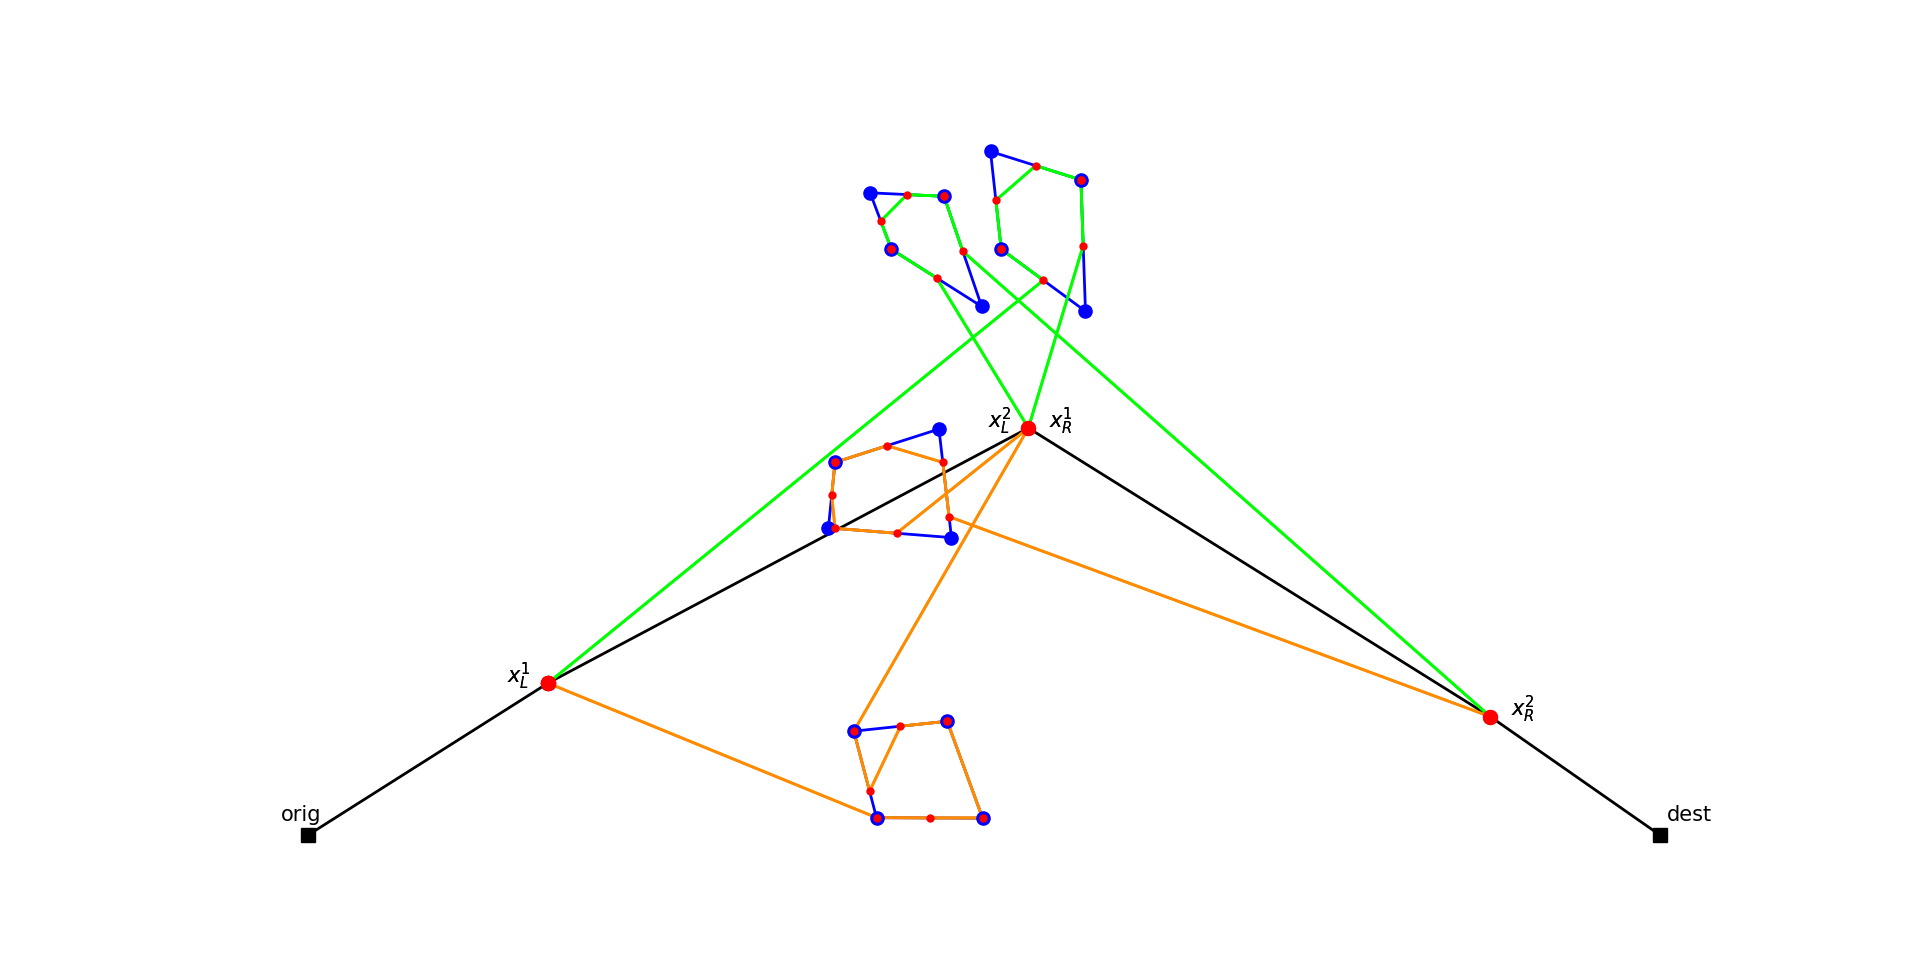
\includegraphics[width=0.95\linewidth]{figures/figure_latex.png}
% \caption{Example illustrating the meaning of the launching  (L) and retrieving (R) points.}
% \label{fig:illustrative}
% \end{figure}

% This file was created with tikzplotlib v0.9.12.
\begin{figure}[h!]
\centering
% This file was created with tikzplotlib v0.9.12.
\begin{tikzpicture}

\definecolor{color0}{rgb}{1,0.549019607843137,0}

\begin{axis}[
hide x axis,
hide y axis,
scaled x ticks=manual:{}{\pgfmathparse{#1}},
scaled y ticks=manual:{}{\pgfmathparse{#1}},
tick align=outside,
x grid style={white!69.0196078431373!black},
xmajorticks=false,
xmin=-5, xmax=105,
xtick style={color=black},
xticklabels={},
y grid style={white!69.0196078431373!black},
ymajorticks=false,
ymin=-5, ymax=75,
ytick style={color=black},
yticklabels={}
]
\path [draw=blue, thick]
(axis cs:21.0696182692914,1.38670279952717)
--(axis cs:30.306045132353,1.50447958089156);

\path [draw=blue, thick]
(axis cs:21.0696182692914,1.38670279952717)
--(axis cs:23.9355243392435,8.22107815581281);

\path [draw=blue, thick]
(axis cs:30.306045132353,1.50447958089156)
--(axis cs:30.6007400849981,8.61180925900065);

\path [draw=blue, thick]
(axis cs:23.9355243392435,8.22107815581281)
--(axis cs:30.6007400849981,8.61180925900065);

\path [draw=blue, thick]
(axis cs:4.08370396767994,62.5193171258523)
--(axis cs:8.09069545603466,60.4417973648425);

\path [draw=blue, thick]
(axis cs:4.08370396767994,62.5193171258523)
--(axis cs:2.37426610997379,66.9905560181573);

\path [draw=blue, thick]
(axis cs:8.09069545603466,60.4417973648425)
--(axis cs:8.40433589338944,70.7975020391092);

\path [draw=blue, thick]
(axis cs:2.37426610997379,66.9905560181573)
--(axis cs:8.40433589338944,70.7975020391092);

\path [draw=blue, thick]
(axis cs:21.0664581490033,38.3255279820558)
--(axis cs:29.0472438012912,42.369596955967);

\path [draw=blue, thick]
(axis cs:21.0664581490033,38.3255279820558)
--(axis cs:22.1750046919912,47.5858849832036);

\path [draw=blue, thick]
(axis cs:29.0472438012912,42.369596955967)
--(axis cs:27.0356718607916,49.5164362980235);

\path [draw=blue, thick]
(axis cs:22.1750046919912,47.5858849832036)
--(axis cs:27.0356718607916,49.5164362980235);

\path [draw=blue, thick]
(axis cs:89.6170857784204,29.8130206242151)
--(axis cs:98.4204942730176,31.9280359170996);

\path [draw=blue, thick]
(axis cs:89.6170857784204,29.8130206242151)
--(axis cs:89.5168058385155,39.6742972814671);

\path [draw=blue, thick]
(axis cs:98.4204942730176,31.9280359170996)
--(axis cs:97.2556927544101,39.0446066906692);

\path [draw=blue, thick]
(axis cs:89.5168058385155,39.6742972814671)
--(axis cs:97.2556927544101,39.0446066906692);

\path [draw=black, thick]
(axis cs:0,0)
--(axis cs:0,0)
--(axis cs:11.9384375817266,38.1768740390765)
--(axis cs:10.3131414759248,47.5858849832036)
--(axis cs:44.9451427093311,40.8090894507933)
--(axis cs:64.0827735142413,29.8198845110857)
--(axis cs:95.4029040306271,4.93918065109767)
--(axis cs:100,0);
\path [draw=green, thick]
(axis cs:0,0)
--(axis cs:21.0696182692914,1.38670279952717)
--(axis cs:25.6878317008222,1.44559119020937)
--(axis cs:30.3792241725836,3.26938108252212)
--(axis cs:30.5265716489061,6.82304592157666)
--(axis cs:27.2681322121208,8.41644370740673)
--(axis cs:23.9355243392435,8.22107815581281)
--(axis cs:23.9355243392435,8.22107815581281)
--(axis cs:22.5025713042674,4.80389047767)
--(axis cs:11.9384375817266,38.1768740390765);
\path [draw=color0, thick]
(axis cs:0,0)
--(axis cs:21.0664581490033,38.3255279820558)
--(axis cs:25.0568509751472,40.3475624690114)
--(axis cs:29.0472438012912,42.369596955967)
--(axis cs:28.0414578310414,45.9430166269952)
--(axis cs:24.6053382763914,48.5511606406136)
--(axis cs:22.1750046919912,47.5858849832036)
--(axis cs:22.1750046919912,47.5858849832036)
--(axis cs:21.3637623976544,40.8090894507933)
--(axis cs:11.9384375817266,38.1768740390765);
\path [draw=green, thick]
(axis cs:0,0)
--(axis cs:21.0696182692914,1.38670279952717)
--(axis cs:25.6878317008222,1.44559119020937)
--(axis cs:30.3792241725836,3.26938108252212)
--(axis cs:30.5265716489061,6.82304592157666)
--(axis cs:27.2681322121208,8.41644370740673)
--(axis cs:23.9355243392435,8.22107815581281)
--(axis cs:23.9355243392435,8.22107815581281)
--(axis cs:22.5025713042674,4.80389047767)
--(axis cs:11.9384375817266,38.1768740390765);
\path [draw=color0, thick]
(axis cs:0,0)
--(axis cs:21.0664581490033,38.3255279820558)
--(axis cs:25.0568509751472,40.3475624690114)
--(axis cs:29.0472438012912,42.369596955967)
--(axis cs:28.0414578310414,45.9430166269952)
--(axis cs:24.6053382763914,48.5511606406136)
--(axis cs:22.1750046919912,47.5858849832036)
--(axis cs:22.1750046919912,47.5858849832036)
--(axis cs:21.3637623976544,40.8090894507933)
--(axis cs:11.9384375817266,38.1768740390765);
\path [draw=green, thick]
(axis cs:10.3131414759248,47.5858849832036)
--(axis cs:8.09069545603467,60.4417973648425)
--(axis cs:6.08719971185731,61.4805572453474)
--(axis cs:8.1475539671049,62.3191380350312)
--(axis cs:8.30437418578229,67.4969903721645)
--(axis cs:5.38930100168162,68.8940290286332)
--(axis cs:2.37426610997379,66.9905560181573)
--(axis cs:2.3742661099738,66.9905560181572)
--(axis cs:3.22898503882687,64.7549365720048)
--(axis cs:44.9451427093311,40.8090894507933);
\path [draw=green, thick]
(axis cs:10.3131414759248,47.5858849832036)
--(axis cs:8.09069545603467,60.4417973648425)
--(axis cs:6.08719971185731,61.4805572453474)
--(axis cs:8.1475539671049,62.3191380350312)
--(axis cs:8.30437418578229,67.4969903721645)
--(axis cs:5.38930100168162,68.8940290286332)
--(axis cs:2.37426610997379,66.9905560181573)
--(axis cs:2.3742661099738,66.9905560181572)
--(axis cs:3.22898503882687,64.7549365720048)
--(axis cs:44.9451427093311,40.8090894507933);
\path [draw=green, thick]
(axis cs:64.0827735142413,29.8198845110857)
--(axis cs:89.6170857784204,29.8130206242151)
--(axis cs:94.018790025719,30.8705282706573)
--(axis cs:97.8380935137139,35.4863213038844)
--(axis cs:97.2556927544101,39.0446066906692)
--(axis cs:97.25569275441,39.0446066906692)
--(axis cs:93.3862492964628,39.3594519860681)
--(axis cs:89.5669458084679,34.7436589528409)
--(axis cs:89.6170857784204,29.8130206242149)
--(axis cs:95.4029040306271,4.93918065109767);
\path [draw=green, thick]
(axis cs:64.0827735142413,29.8198845110857)
--(axis cs:89.6170857784204,29.8130206242151)
--(axis cs:94.018790025719,30.8705282706573)
--(axis cs:97.8380935137139,35.4863213038844)
--(axis cs:97.2556927544101,39.0446066906692)
--(axis cs:97.25569275441,39.0446066906692)
--(axis cs:93.3862492964628,39.3594519860681)
--(axis cs:89.5669458084679,34.7436589528409)
--(axis cs:89.6170857784204,29.8130206242149)
--(axis cs:95.4029040306271,4.93918065109767);
\addplot [draw=blue, fill=blue, mark=*, only marks]
table{%
x  y
21.0696182692914 1.38670279952717
30.306045132353 1.50447958089156
23.9355243392435 8.22107815581281
30.6007400849981 8.61180925900065
};
\addplot [draw=blue, fill=blue, mark=*, only marks]
table{%
x  y
4.08370396767994 62.5193171258523
8.09069545603466 60.4417973648425
2.37426610997379 66.9905560181573
8.40433589338944 70.7975020391092
};
\addplot [draw=blue, fill=blue, mark=*, only marks]
table{%
x  y
21.0664581490033 38.3255279820558
29.0472438012912 42.369596955967
22.1750046919912 47.5858849832036
27.0356718607916 49.5164362980235
};
\addplot [draw=blue, fill=blue, mark=*, only marks]
table{%
x  y
89.6170857784204 29.8130206242151
98.4204942730176 31.9280359170996
89.5168058385155 39.6742972814671
97.2556927544101 39.0446066906692
};
\addplot [semithick, red, mark=*, mark size=1, mark options={solid}, only marks]
table {%
25.6878317008222 1.44559119020937
21.0696182692914 1.38670279952717
23.9355243392435 8.22107815581281
22.5025713042674 4.80389047767
30.3792241725836 3.26938108252212
30.5265716489061 6.82304592157666
27.2681322121208 8.41644370740673
23.9355243392435 8.22107815581281
8.09069545603467 60.4417973648425
6.08719971185731 61.4805572453474
2.3742661099738 66.9905560181572
3.22898503882687 64.7549365720048
8.1475539671049 62.3191380350312
8.30437418578229 67.4969903721645
5.38930100168162 68.8940290286332
2.37426610997379 66.9905560181573
21.0664581490033 38.3255279820558
25.0568509751472 40.3475624690114
22.1750046919912 47.5858849832036
21.3637623976544 40.8090894507933
29.0472438012912 42.369596955967
28.0414578310414 45.9430166269952
24.6053382763914 48.5511606406136
22.1750046919912 47.5858849832036
89.6170857784204 29.8130206242151
94.018790025719 30.8705282706573
89.5669458084679 34.7436589528409
89.6170857784204 29.8130206242149
97.8380935137139 35.4863213038844
97.2556927544101 39.0446066906692
97.25569275441 39.0446066906692
93.3862492964628 39.3594519860681
};
\addplot [semithick, black, opacity=1, mark=square*, mark size=2.5, mark options={solid}, only marks]
table {%
0 0
100 0
};
\addplot [semithick, red, opacity=1, mark=*, mark size=1.5, mark options={solid}, only marks]
table {%
0 0
11.9384375817266 38.1768740390765
10.313141475924828 47.585884983203592
44.9451427093311 40.8090894507933
64.082773514241339 29.819884511085665
95.4029040306271 4.93918065109767
};
\draw (0,10) node[
  scale=0.75,
  anchor=base west,
  text=black,
  rotate=0.0
]{origin};
\draw (0,10) node[
  scale=0.75,
  anchor=base west,
  text=black,
  rotate=0.0
]{origin};
\draw (axis cs:3.4384375817266,38.1768740390765) node[
  scale=0.75,
  anchor=base west,
  text=black,
  rotate=0.0
]{$x_R^1$};
\draw (axis cs:2,3) node[
  scale=0.75,
  anchor=base west,
  text=black,
  rotate=0.0
]{$x_L^1$};
\draw (axis cs:3.4384375817266,38.1768740390765) node[
  scale=0.75,
  anchor=base west,
  text=black,
  rotate=0.0
]{$x_R^1$};
\draw (axis cs:2,3) node[
  scale=0.75,
  anchor=base west,
  text=black,
  rotate=0.0
]{$x_L^1$};
\draw (axis cs:46.4451427093311,40.8090894507933) node[
  scale=0.75,
  anchor=base west,
  text=black,
  rotate=0.0
]{$x_R^2$};
\draw (axis cs:2.7,47.5858849832036) node[
  scale=0.75,
  anchor=base west,
  text=black,
  rotate=0.0
]{$x_L^2$};
\draw (axis cs:46.4451427093311,40.8090894507933) node[
  scale=0.75,
  anchor=base west,
  text=black,
  rotate=0.0
]{$x_R^2$};
\draw (axis cs:2.7,47.5858849832036) node[
  scale=0.75,
  anchor=base west,
  text=black,
  rotate=0.0
]{$x_L^2$};
\draw (axis cs:86,1) node[
  scale=0.75,
  anchor=base west,
  text=black,
  rotate=0.0
]{$x_R^3$};
\draw (axis cs:55.0827735142413,27) node[
  scale=0.75,
  anchor=base west,
  text=black,
  rotate=0.0
]{$x_L^3$};
\draw (axis cs:86,1) node[
  scale=0.75,
  anchor=base west,
  text=black,
  rotate=0.0
]{$x_R^3$};
\draw (axis cs:55.0827735142413,27) node[
  scale=0.75,
  anchor=base west,
  text=black,
  rotate=0.0
]{$x_L^3$};
\draw (100, 10) node[
  scale=0.75,
  anchor=base west,
  text=black,
  rotate=0.0
]{dest};
\draw (100, 10) node[
  scale=0.75,
  anchor=base west,
  text=black,
  rotate=0.0
]{dest};
\end{axis}
\end{tikzpicture}
\subcaption{[a]}
\begin{tikzpicture}
\definecolor{color0}{rgb}{1,0.549019607843137,0}
\begin{axis}[
hide x axis,
hide y axis,
scaled x ticks=manual:{}{\pgfmathparse{#1}},
scaled y ticks=manual:{}{\pgfmathparse{#1}},
tick align=outside,
x grid style={white!69.0196078431373!black},
xmajorticks=false,
xmin=-5, xmax=105,
xtick style={color=black},
xticklabels={},
y grid style={white!69.0196078431373!black},
ymajorticks=false,
ymin=-5, ymax=75,
ytick style={color=black},
yticklabels={}
]
\path [draw=blue, thick]
(axis cs:21.0696182692914,1.38670279952717)
--(axis cs:30.306045132353,1.50447958089156);

\path [draw=blue, thick]
(axis cs:21.0696182692914,1.38670279952717)
--(axis cs:23.9355243392435,8.22107815581281);

\path [draw=blue, thick]
(axis cs:30.306045132353,1.50447958089156)
--(axis cs:30.6007400849981,8.61180925900065);

\path [draw=blue, thick]
(axis cs:23.9355243392435,8.22107815581281)
--(axis cs:30.6007400849981,8.61180925900065);

\path [draw=blue, thick]
(axis cs:4.08370396767994,62.5193171258523)
--(axis cs:8.09069545603466,60.4417973648425);

\path [draw=blue, thick]
(axis cs:4.08370396767994,62.5193171258523)
--(axis cs:2.37426610997379,66.9905560181573);

\path [draw=blue, thick]
(axis cs:8.09069545603466,60.4417973648425)
--(axis cs:8.40433589338944,70.7975020391092);

\path [draw=blue, thick]
(axis cs:2.37426610997379,66.9905560181573)
--(axis cs:8.40433589338944,70.7975020391092);

\path [draw=blue, thick]
(axis cs:21.0664581490033,38.3255279820558)
--(axis cs:29.0472438012912,42.369596955967);

\path [draw=blue, thick]
(axis cs:21.0664581490033,38.3255279820558)
--(axis cs:22.1750046919912,47.5858849832036);

\path [draw=blue, thick]
(axis cs:29.0472438012912,42.369596955967)
--(axis cs:27.0356718607916,49.5164362980235);

\path [draw=blue, thick]
(axis cs:22.1750046919912,47.5858849832036)
--(axis cs:27.0356718607916,49.5164362980235);

\path [draw=blue, thick]
(axis cs:89.6170857784204,29.8130206242151)
--(axis cs:98.4204942730176,31.9280359170996);

\path [draw=blue, thick]
(axis cs:89.6170857784204,29.8130206242151)
--(axis cs:89.5168058385155,39.6742972814671);

\path [draw=blue, thick]
(axis cs:98.4204942730176,31.9280359170996)
--(axis cs:97.2556927544101,39.0446066906692);

\path [draw=blue, thick]
(axis cs:89.5168058385155,39.6742972814671)
--(axis cs:97.2556927544101,39.0446066906692);

\path [draw=black, thick]
(axis cs:0,0)
--(axis cs:5.19517108668237e-05,5.19721988422751e-05)
--(axis cs:8.31804668177588,39.1256215879103)
--(axis cs:8.0902667404291,41.3992381927182)
--(axis cs:41.9928361091472,39.3784823234059)
--(axis cs:61.5718673452208,26.0879192386296)
--(axis cs:94.5456634712005,3.70413789044963)
--(axis cs:100,0);
\path [draw=green, thick]
(axis cs:5.19517108668237e-05,5.19721988422751e-05)
--(axis cs:21.0696185355958,1.3867034345879)
--(axis cs:22.5025656416375,4.80387697389931)
--(axis cs:24.9379489929542,1.43602918392242)
--(axis cs:29.5561397992636,1.49491728610282)
--(axis cs:30.353931133669,2.65937414309857)
--(axis cs:30.5012780269027,6.21302491945877)
--(axis cs:29.1826401424249,8.52867680295897)
--(axis cs:25.850065249296,8.33331318471784)
--(axis cs:8.31804668177588,39.1256215879103);
\path [draw=green, thick]
(axis cs:5.19517108668237e-05,5.19721988422751e-05)
--(axis cs:21.0696185355958,1.3867034345879)
--(axis cs:22.5025656416375,4.80387697389931)
--(axis cs:24.9379489929542,1.43602918392242)
--(axis cs:29.5561397992636,1.49491728610282)
--(axis cs:30.353931133669,2.65937414309857)
--(axis cs:30.5012780269027,6.21302491945877)
--(axis cs:29.1826401424249,8.52867680295897)
--(axis cs:25.850065249296,8.33331318471784)
--(axis cs:8.31804668177588,39.1256215879103);
\path [draw=green, thick]
(axis cs:8.0902667404291,41.3992381927182)
--(axis cs:6.08717590107675,61.4805695906112)
--(axis cs:4.0837005407278,62.5193189026369)
--(axis cs:4.08369465698464,62.5193414790879)
--(axis cs:3.22897670117108,64.7549583801393)
--(axis cs:2.84174575638185,67.2856885528858)
--(axis cs:5.85674978390742,69.1891420779693)
--(axis cs:8.3052804744899,67.5269139951667)
--(axis cs:8.14846106263484,62.3490882974996)
--(axis cs:41.9928361091472,39.3784823234059);
\path [draw=color0, thick]
(axis cs:8.0902667404291,41.3992381927182)
--(axis cs:27.6728191506586,47.2527393224256)
--(axis cs:28.7000788954416,43.6030262742796)
--(axis cs:24.4315739690114,40.0307185577996)
--(axis cs:28.4696719165738,42.0769264544708)
--(axis cs:22.0922910532811,46.8949281369037)
--(axis cs:21.5323008920902,42.2169930131509)
--(axis cs:23.3011399504012,48.0331614224841)
--(axis cs:25.830886920397,49.0379219151249)
--(axis cs:41.9928361091472,39.3784823234059);
\path [draw=green, thick]
(axis cs:8.0902667404291,41.3992381927182)
--(axis cs:6.08717590107675,61.4805695906112)
--(axis cs:4.0837005407278,62.5193189026369)
--(axis cs:4.08369465698464,62.5193414790879)
--(axis cs:3.22897670117108,64.7549583801393)
--(axis cs:2.84174575638185,67.2856885528858)
--(axis cs:5.85674978390742,69.1891420779693)
--(axis cs:8.3052804744899,67.5269139951667)
--(axis cs:8.14846106263484,62.3490882974996)
--(axis cs:41.9928361091472,39.3784823234059);
\path [draw=color0, thick]
(axis cs:8.0902667404291,41.3992381927182)
--(axis cs:27.6728191506586,47.2527393224256)
--(axis cs:28.7000788954416,43.6030262742796)
--(axis cs:24.4315739690114,40.0307185577996)
--(axis cs:28.4696719165738,42.0769264544708)
--(axis cs:22.0922910532811,46.8949281369037)
--(axis cs:21.5323008920902,42.2169930131509)
--(axis cs:23.3011399504012,48.0331614224841)
--(axis cs:25.830886920397,49.0379219151249)
--(axis cs:41.9928361091472,39.3784823234059);
\path [draw=color0, thick]
(axis cs:61.5718673452208,26.0879192386296)
--(axis cs:89.5688132333832,34.5600210912317)
--(axis cs:89.5186458802408,39.4933522137777)
--(axis cs:89.9608257385526,39.6381686810341)
--(axis cs:93.8383627815696,39.3226648342931)
--(axis cs:97.7899505784608,35.7804594900926)
--(axis cs:98.374626227098,32.2082752452751)
--(axis cs:98.3537907014276,31.9120104112867)
--(axis cs:93.9472998319943,30.8533527808329)
--(axis cs:94.5456634712005,3.70413789044963);
\path [draw=color0, thick]
(axis cs:61.5718673452208,26.0879192386296)
--(axis cs:89.5688132333832,34.5600210912317)
--(axis cs:89.5186458802408,39.4933522137777)
--(axis cs:89.9608257385526,39.6381686810341)
--(axis cs:93.8383627815696,39.3226648342931)
--(axis cs:97.7899505784608,35.7804594900926)
--(axis cs:98.374626227098,32.2082752452751)
--(axis cs:98.3537907014276,31.9120104112867)
--(axis cs:93.9472998319943,30.8533527808329)
--(axis cs:94.5456634712005,3.70413789044963);
\addplot [draw=blue, fill=blue, mark=*, only marks]
table{%
x  y
21.0696182692914 1.38670279952717
30.306045132353 1.50447958089156
23.9355243392435 8.22107815581281
30.6007400849981 8.61180925900065
};
\addplot [draw=blue, fill=blue, mark=*, only marks]
table{%
x  y
4.08370396767994 62.5193171258523
8.09069545603466 60.4417973648425
2.37426610997379 66.9905560181573
8.40433589338944 70.7975020391092
};
\addplot [draw=blue, fill=blue, mark=*, only marks]
table{%
x  y
21.0664581490033 38.3255279820558
29.0472438012912 42.369596955967
22.1750046919912 47.5858849832036
27.0356718607916 49.5164362980235
};
\addplot [draw=blue, fill=blue, mark=*, only marks]
table{%
x  y
89.6170857784204 29.8130206242151
98.4204942730176 31.9280359170996
89.5168058385155 39.6742972814671
97.2556927544101 39.0446066906692
};
\addplot [semithick, red, mark=*, mark size=1, mark options={solid}, only marks]
table {%
24.9379489929542 1.43602918392242
29.5561397992636 1.49491728610282
21.0696185355958 1.3867034345879
22.5025656416375 4.80387697389931
30.353931133669 2.65937414309857
30.5012780269027 6.21302491945877
29.1826401424249 8.52867680295897
25.850065249296 8.33331318471784
6.08717590107675 61.4805695906112
4.0837005407278 62.5193189026369
4.08369465698464 62.5193414790879
3.22897670117108 64.7549583801393
8.3052804744899 67.5269139951667
8.14846106263484 62.3490882974996
2.84174575638185 67.2856885528858
5.85674978390742 69.1891420779693
24.4315739690114 40.0307185577996
28.4696719165738 42.0769264544708
22.0922910532811 46.8949281369037
21.5323008920902 42.2169930131509
27.6728191506586 47.2527393224256
28.7000788954416 43.6030262742796
23.3011399504012 48.0331614224841
25.830886920397 49.0379219151249
98.3537907014276 31.9120104112867
93.9472998319943 30.8533527808329
89.5688132333832 34.5600210912317
89.5186458802408 39.4933522137777
97.7899505784608 35.7804594900926
98.374626227098 32.2082752452751
89.9608257385526 39.6381686810341
93.8383627815696 39.3226648342931
};

\addplot [semithick, black, opacity=1, mark=square*, mark size=2.5, mark options={solid}, only marks]
table {%
0 0
100 0
};
\addplot [semithick, red, opacity=1, mark=*, mark size=1.5, mark options={solid}, only marks]
table {%
5.19517108668237e-05 5.19721988422751e-05
8.31804668177588 39.1256215879103
8.0902667404291044 41.399238192718173
41.9928361091472 39.3784823234059
61.571867345220838 26.087919238629631
94.5456634712005 3.70413789044963
};
\draw (0, 10) node[
  scale=0.75,
  anchor=base west,
  text=black,
  rotate=0.0
]{origin};
\draw (axis cs:2,3) node[
  scale=0.75,
  anchor=base west,
  text=black,
  rotate=0.0
]{$x_L^1$};
\draw (axis cs:0,36) node[
  scale=0.75,
  anchor=base west,
  text=black,
  rotate=0.0
]{$x_R^1$};
\draw (axis cs:0,44) node[
  scale=0.75,
  anchor=base west,
  text=black,
  rotate=0.0
]{$x_L^2$};
\draw (axis cs:43.4928361091472,39.3784823234059) node[
  scale=0.75,
  anchor=base west,
  text=black,
  rotate=0.0
]{$x_R^2$};
\draw (axis cs:53,23) node[
  scale=0.75,
  anchor=base west,
  text=black,
  rotate=0.0
]{$x_L^3$};
\draw (axis cs:85,0) node[
  scale=0.75,
  anchor=base west,
  text=black,
  rotate=0.0
]{$x_R^3$};
\draw (100,10) node[
  scale=0.75,
  anchor=base west,
  text=black,
  rotate=0.0
]{dest};
\draw (0, 10) node[
  scale=0.75,
  anchor=base west,
  text=black,
  rotate=0.0
]{origin};
\draw (axis cs:2,3) node[
  scale=0.75,
  anchor=base west,
  text=black,
  rotate=0.0
]{$x_L^1$};
\draw (axis cs:0,36) node[
  scale=0.75,
  anchor=base west,
  text=black,
  rotate=0.0
]{$x_R^1$};
\draw (axis cs:0,44) node[
  scale=0.75,
  anchor=base west,
  text=black,
  rotate=0.0
]{$x_L^2$};
\draw (axis cs:43.4928361091472,39.3784823234059) node[
  scale=0.75,
  anchor=base west,
  text=black,
  rotate=0.0
]{$x_R^2$};
\draw (axis cs:53,23) node[
  scale=0.75,
  anchor=base west,
  text=black,
  rotate=0.0
]{$x_L^3$};
\draw (axis cs:85,0) node[
  scale=0.75,
  anchor=base west,
  text=black,
  rotate=0.0
]{$x_R^3$};
\draw (100,10) node[
  scale=0.75,
  anchor=base west,
  text=black,
  rotate=0.0
]{dest};
\end{axis}
\end{tikzpicture}
\subcaption{[b]}
\caption{Example of feasible solution [a] and optimal solution [b] for a problem instance with 4 graphs and 2 drones.}
\label{fig:illustrative}
\end{figure}
\noindent
Figure \ref{fig:illustrative} shows an example of the notation over a configuration with four target graphs that have four nodes and four edges. Here, it is supposed that the number of available drones is equal to two. %: one with six nodes and 7 edges and the other one with four nodes and edges%. 
\LA{In particular, figure \ref{fig:illustrative}[a] represents a feasible solution of the problem for this configuration.
The mothership begins at its starting point $orig$ which coincides with the first launching point $x_L^1$ where two drones (the green one and the orange one) are launched to visit two graphs. There, each drone follows a route (represented by the orange and green paths) that ensures the coverage of \RE{one half of the length of} each edge of the graph. The red dots on the visited graphs are the intermediate points $R^{e_g}$ and $L^{e_g}$ used by the drones in their visit to the edges of the different graphs. After finishing the visit of the first two graphs\RE{,} the drones return to the point $x_R^1$. The mothership moves from this point to the second launching point $x_L^2$ from where only one drone (the green one) is launched to visit the third graph. Once this graph is visited, the drone returns to the mothership at the rendezvous point $x_R^2$. Finally, the mothership moves to the point $x_L^3$ from where one drone is launched for the last visit to the fourth graph. Then, the drone is retrieved by the mothership at the point $x_R^3$ and then the mothership ends its route at the destination point $dest$.\\
Figure \ref{fig:illustrative}[b] represents the optimal solution for the same instance of the problem. We can observe that, in this case, from the first launching point $x_L^1$ only one drone is launched, while from the second $x_L^2$ two drones are launched to visit the second and the third graph. The different position in the space of this latter point, with respect to the feasible solution reported in figure \ref{fig:illustrative}[a] whose total time is 158.36, ensures that the total traveling time of the optimal solution equals to 152.39, which is shorter.}


% \JP{ ************************ 

% TO BE INSERTED: An example showing the notation with a figure...  Please Carlos insert something similar to what we use in the previous paper (JUSTO dixit)

%      ************************}
\noindent
To include the definition of these paths in our mathematical programming formulation\RE{,} we need to make decisions to choose:
\begin{itemize}
    \item The optimal assignment of drones for visiting graphs in a given \RE{operation $o$}.
    \item The order to visit the edges of each graph in its corresponding \RE{operation}.
\end{itemize}

% Binary variables
% Thus, to this end one can define the following binary variables:

\subsubsection*{Drone Constraints}
\noindent
We model the route that the drone follows by using the binary variables $u^{e_go}$, $z^{e_ge^\prime_g}$ and $v^{e_go}$ defined in Table \ref{table:t2}.


% \begin{itemize}
%   \item $u^{{e_g}td} = 1$ if the visit of graph $g$ is done at stage $t$ by the drone $d$ and it starts from edge $e_g$.
%   \item $v^{{e_g}td}= 1$ if the visit of graph $g$ that is done by drone $d$ at stage $t$ finishes in the edge $e_g$.
%   \item $z^{e_ge'_g}= 1$ if the drone moves from edge $e_g$ to $e'_g$ while visiting the graph $g$.
% \end{itemize}

% By using these binary variables, we can model the route that follows the drone:
\begin{align}
    % \sum_{g\in \mathcal G}\sum_{e_g\in E_g} \sum_{d\in\mathcal D} u^{e_gtd} & \leq 1, &\forall t\in \mathcal T, \label{st:DEnt}\\%\tag{DEn}\\
    % \sum_{g\in\mathcal G}\sum_{e_g\in E_g} \sum_{d\in\mathcal D} v^{e_gtd} & \leq 1, &\forall t\in \mathcal T, \label{st:DExt}\\%\tag{DEx}\\
    \sum_{g\in \mathcal G}\sum_{e_g\in E_g}  u^{e_go} & \leq \RE{|\mathcal D|}, &\forall o\in \mathcal O,\label{st:DEnt}\\
    \sum_{g\in \mathcal G}\sum_{e_g\in E_g}  v^{e_go} & \leq \RE{|\mathcal D|}, &\forall o\in \mathcal O,\label{st:DExt} \\
    \sum_{e_g\in E_g} \sum_{o\in \mathcal O} u^{e_go} & = 1, &\forall g\in\mathcal G, \label{st:DEng}\\%\tag{D
    \sum_{e_g\in E_g} \sum_{o\in \mathcal O} v^{e_go} & = 1, &\forall g\in\mathcal G, \label{st:DExg}\\%\tag{D
    \sum_{e_g\in E_g} u^{e_go} & = \sum_{e_g\in E_g} v^{e_go}, &\forall g\in\mathcal G, \forall o\in \mathcal O, \label{st:Duv}\\%\tag{D
     \sum_{o\in \mathcal O} u^{e_go} + \sum_{e^\prime_g\in E_g} z_g^{e^\prime_ge_g} & = \mu^{e_g}, &\forall e_g\in E_g:g\in\mathcal G, \label{st:DInu}\\
     \sum_{o\in \mathcal O} v^{e_go} + \sum_{e^\prime_g\in E_g} z_g^{e_ge^\prime_g} & = \mu^{e_g}, &\forall e_g\in E_g:g\in\mathcal G. \label{st:DInv}
\end{align}

\noindent 
\RE{\CV{Inequalities \eqref{st:DEnt} and \eqref{st:DExt} state that it is not possible to use a number of drones bigger than the available one at each operation $o$.}}  Constraints \eqref{st:DEng} and \eqref{st:DExg} assure that each graph is visited at some \RE{operation $o$} by some drone. Equations \eqref{st:Duv} ensure that the \RE{action} of entering and exiting from the graph $g$ occurs in the same \RE{operation $o$}. Constraints \eqref{st:DInu} state that if \RE{an} edge $e$ of graph $g$ is visited by a drone, one of two alternative situations must occur: either $e$ is the first edge of graph $g$ visited by the drone at \RE{operation $o$}, or edge $e$ is visited by the drone after visiting another edge $e^\prime$ of graph $g$. Similarly, constraints \eqref{st:DInv} state that if \RE{an} edge $e$ of graph $g$ is visited by a drone, either $e$ is the last edge of graph $g$ visited by the drone at \RE{operation $o$}, or the drone must move to another edge $e^\prime$ of graph $g$ after visiting edge $e$.

\subsubsection*{Distance and Time Constraints}
\noindent
The goal of the \AMDCO\xspace is to find a feasible solution that minimizes the total \RE{time} traveled by the mothership. To account for the different distances \RE{between} the decision variables of the model we need to set the continuous variables $d_L^{e_go}$, $d^{e_g}$, $d^{e_ge^\prime_g}$, $d_R^{e_go}$, $d_{orig}$, $d_{RL}^o$, $d_{LR}^o$ and $d_{dest}$ defined in Table \ref{table:t2}. This can be done by means of the following constraints:

\begin{align*}
\|x_L^o- R^{e_g}\| & \leq  d_L^{e_go},  &\forall e_g\in E_g:g\in \mathcal{G}, \:\:\forall o\in \mathcal O, \tag{Drone DIST$_{1}$-CO} \label{eq:drone-d1-async-CO}\\
\|R^{e_g}- L^{e_g}\| & \leq  d^{e_g},  &\forall e_g\in E_g:g\in \mathcal{G}, \tag{Drone DIST$_{2}$-CO} \label{eq:drone-d2-async-CO}\\
\|R^{e_g}- L^{e'_g}\| & \leq  d^{e_ge'_g}, &\forall e_g\neq e_g'\in E_g:g\in \mathcal{G}, \tag{Drone DIST$_{3}$-CO} \label{eq:drone-d3-async-CO}\\
\|L^{e_g}- x_R^o\| & \leq  d_R^{e_o}, &\forall e_g\in E_g:g\in \mathcal{G},\:\:\forall o\in \mathcal O. \tag{Drone DIST$_{4}$-CO} \label{eq:drone-d4-async-CO}\\\\
\|orig - x_L^1\| & \leq d_{orig}, \tag{Mothership DIST$_1$-CO}\label{eq:mothership-d1-async-CO}\\
\|x_L^o - x_R^{o}\| & \leq d_{LR}^{o}, &\forall o\in\mathcal O, \tag{Mothership DIST$_{2}$-CO}\label{eq:mothership-d3-async-CO}\\
\|x_R^o - x_L^{o+1}\| & \leq d_{RL}^{o}, &\forall o\in\mathcal O:o<|\mathcal O|, \tag{Mothership DIST$_{3}$-CO}\label{eq:mothership-d4-async-CO}\\
\|x_R^{|\mathcal O|} - dest\| & \leq d_{dest}. \tag{Mothership DIST$_4$-CO}\label{eq:mothership-d6-async-CO}
\end{align*}

\noindent
All variables modelling \RE{the} distances covered by drones, namely $d_L^{e_go}$, $d^{e_g}$, $d^{e_g'e_g}$ and $d_R^{e_go}$,  as well as those modelling the distance travelled by the mothership, namely $d_{orig}$, $d_{LR}^o$, $d_{RL}^o$ and $d_{dest}$, are defined in \JP{Table \ref{table:t2}.} 
 
 
 
\begin{comment}
\begin{align*}
\|x_L^o- R^{e_g}\| & \leq  d_L^{e_go},  &\quad \forall e_g:g\in \mathcal{G}, \forall o\in \mathcal O, \tag{DIST$_{1}$-o} \label{eq:d1}\\
\|R^{e_g}- L^{e_g}\| & \leq  d^{e_g},  &\quad \forall e_g:g\in \mathcal{G}, \tag{DIST$_{2}$-o} \label{eq:d2}\\
\|R^{e_g}- L^{e^\prime_g}\| & \leq  d^{e_ge^\prime_g}, &\quad \forall e_g\neq e_g'\in E_g:g\in \mathcal{G}, \tag{DIST$_{3}$-o} \label{eq:d3}\\
\|L^{e_g}- x_R^o\| & \leq  d_R^{e_go}, &\quad \forall e_g:g\in \mathcal{G},\forall o\in \mathcal O, \tag{DIST$_{4}$-o} \label{eq:d4}\\
\|x_R^o- x_L^{o+1}\| & \leq  d_{RL}^o, & \quad \forall o\in \mathcal O\CV{\setminus |\mathcal O|}, \tag{DIST$_{5}$-o} \label{eq:d5}\\
\|x_L^o- x_R^o\| & \leq  d_{LR}^o, & \quad \forall o\in \mathcal O. \tag{DIST$_{6}$-o} \label{eq:d6}\\
\end{align*}
\end{comment}

\RE{
\noindent
In order to compute the maximum time spent by a drone to visit a graph $g \in \mathcal G$ associated with operation $o,\forall o \in \mathcal O$, we introduce the following constraints:

\begin{equation}\tag{Time$_D^o$}
time_D^o \geq \frac{1}{v_D}\left(\sum_{e_g\in E_g} u^{e_go}d_L^{e_go} + \sum_{e_g, e^\prime_g\in E_g}z^{e_ge^\prime_g}d^{e_ge^\prime_g} + \sum_{e_g\in E_g} \mu^{e_g}d^{e_g} + \sum_{e_g\in E_g} v^{e_go}d_R^{e_go}\right) - \CV{N_D}(1 - \sum_{e_g\in E_g} u^{e_go}). %\:\: \forall g \in \mathcal G \:\: \forall o \in \mathcal O
\label{eq:timeD}
\end{equation}
\noindent
The first addend within the brackets accounts for the time spent by the drone to go from the launching point $x_L^o$ to the first retrieving point in the graph $R^{e_g}$. The second addend considers the time consumed by the drone to go from edge $e_g$ to $e_g'$ in the graph $g$. The third one computes the time required for traversing the required edges in $g$. The fourth one measures the time to travel from the last launching point $L^{e_g''}$ to the retrieving point $x_R^o$. \CV{Note that, in the special case where all edges must be visited, the third sum of the right-hand side of the \eqref{eq:timeD} constraint, reduces to $\sum_{e_g\in E_g} d^{e_g}$ by setting all the $\mu^{e_g}$ variables equal to one.}
\noindent
The \CV{endurance} term in constraint (\ref{eq:timeD}) ensures that the constraint becomes active only when a graph $g$ is visited during operation $o$. \CV{The reader may observe that the endurance constraint \eqref{CAP} restricts the time spent by the drone to perform operation $o$ to be less than the endurance $N_D$. Therefore, the constant $N_D$ can be taken as the bigM term in \eqref{eq:timeD} constraint.}
\noindent
Note that, to deal with the bilinear terms of the \eqref{eq:timeD} constraint, we use McCormick's envelope to linearize them by adding variables $p\geq 0$  representing the products and introducing the following constraints:
\begin{align*}
    p & \leq  M z, \\
    p & \leq  d, \\
    p & \geq m z, \\
    p & \geq d - M(1 - z),
\end{align*}
where $m$ and $M$ are, respectively, the lower and upper bounds of the distance variable $d$. These bounds will be adjusted for each bilinear term in Section \ref{bounds}.

\noindent
Constraint (\ref{eq:timeMO}) defines the time spent by the mothership to go from the launching point $x_L^o$ to the retrieving point $x_R^o$ associated with operation $o$.

\begin{equation}\tag{Time$_M^o$}
time_M^o = \frac{d_{LR}^o}{v_M}, \quad \forall o \in \mathcal O.
\label{eq:timeMO}
\end{equation}

\noindent
Thus, the overall time spent by the mothership to move from the origin to the destination can be expressed as follows:

\begin{equation}\tag{Time$_M$}
time_M = \frac{1}{v_M} (d_{orig} + \sum_{o \in \mathcal O} d_{LR}^o + \CV{\sum_{o \in \mathcal O:o<|\mathcal O|} d_{RL}^o} + d_{dest}).
\label{eq:timeM}
\end{equation}



\subsubsection*{Coordination and Endurance Constraints}
\noindent
The coordination between the drones and the mothership must ensure that the maximum time $time_D^o$ spent by a drone to visit a graph $g$ at \RE{operation $o$} is less than or equal to the time that the mothership needs to move from the launching point to the retrieving point during \RE{operation $o$}. To this end, we need to define the following coordination constraint for each operation $o\in \mathcal O$:

\begin{equation}\tag{DCW-CO}\label{DCW}
time_D^o \leq time_M^o.
\end{equation}



\noindent
We can model the time endurance constraint for a particular \RE{operation $o\in \mathcal O$} by limiting the time traveled by the drone for this \RE{operation $o$}:

\begin{equation}\tag{Endurance-CO}\label{CAP}
    time_D^o \leq N_D.
\end{equation}


\subsubsection*{AMMDRPG-Complete Overlapping Formulation}
\noindent
Putting together all the constraints introduced before, the following formulation minimizes the \RE{total time} traveled by the mothership\RE{,} ensuring the coordination with the fleet of drones while guaranteeing the required coverage of the target graphs.
\begin{mini*}|s|
 {}{time_M}{}{} \label{AMMDRPG} \tag{AMMDRPG-Complete Overlapping}
  \addConstraint{\eqref{eq:alpha-E} \text{ or } \eqref{eq:alpha-G}}{}{}
  \addConstraint{\eqref{MTZ1}-\eqref{MTZ2}} \text{ or }  \eqref{SEC}
 \addConstraint{\eqref{st:DEnt}-\eqref{st:DInv}}{}{}
 \addConstraint{\eqref{eq:drone-d1-async-CO}-\eqref{eq:drone-d4-async-CO}}{}{} \addConstraint{\eqref{eq:mothership-d1-async-CO}-\eqref{eq:mothership-d6-async-CO}}{}{}
 \addConstraint{\eqref{eq:timeD}, \eqref{eq:timeMO}, \eqref{eq:timeM}}{}{}
 \addConstraint{\eqref{DCW}, \eqref{CAP}.}{}{}
\end{mini*}

\noindent
The objective function accounts for the \RE{time} traveled by the mothership. Constraints \eqref{st:DEnt}-\eqref{st:DInv} models the route followed by the \RE{drones}, \eqref{MTZ1} - \eqref{MTZ2} \text{ or } \eqref{SEC} ensure that the displacement of \RE{a drone}  assigned to the target graph $g\in\mathcal G$ is a route, \eqref{eq:alpha-E} \text{ or } \eqref{eq:alpha-G} define what is required in each visit to a target graph. Constraints (\ref{eq:drone-d1-async-CO})-(\ref{eq:drone-d4-async-CO}) set the variables $d_L^{e_go}$, $d^{e_g}$, $d^{e_ge^\prime_g}$, $d_R^{e_go}$.
The mothership distances $d_{RL}^o$ and $d_{LR}^o$, are defined by means of constraints (\ref{eq:mothership-d1-async-CO})-(\ref{eq:mothership-d6-async-CO}). Constraints (\ref{eq:timeD}), (\ref{eq:timeMO}) and (\ref{eq:timeM}) define the traveled times by the drones and the mothership. Finally, constraints (\ref{DCW})-(\ref{CAP}) guarantee that the coordination and drone endurance are satisfied. %\CV{We don't mention the time constraints}\\
}
% Then, the next six constraints model Euclidean distances needed in the model. \\
% \noindent
% Observe that we are assuming constant velocities for the mothership $v_M$ and the drone $v_D$.\\

\begin{table}[h!]
%\tiny
\scriptsize
\centering
%\color{blue}
\begin{tabular}{|l|}
\hline 
\textbf{Binary and Integer Decision Variables}\\
\hline
$\mu^{e_g} \in \{0,1\}, \:\: \forall e_g \in E_g \:\:(g \in \mathcal{G})$: equal to 1 if edge $e$ of graph $g$ (or a portion of it) is visited by the drone, 0 otherwise.\\
$\text{entry}^{e_g} \in \{0,1\}, \:\: \forall e_g \in E_g\:\: (g \in \mathcal{G})$: auxiliary binary variable used for linearizing expressions.\\
$u^{e_g t} \in \{0,1\}, \:\: \forall e_g \in E_g \:\: (g \in \mathcal{G}), \:\: \forall t \in \mathcal T$: equal to 1 if the visit of graph $g$ starts in stage $t$ from edge $e_g$, 0 otherwise.\\
$z^{e_{g}e^{'}_{g}} \in \{0,1\}, \:\: \forall e_g, e_g' \in E_g\:\: (g \in \mathcal{G})$: equal to 1 if the drone goes from $e_g$ to $e^{'}_{g}$, 0 otherwise.\\
\RE{$\gamma^{gt}\in \{0,1\}, \:\: \forall g\in\mathcal G,\:\:\forall t\in \mathcal T$: equal to 1 if the operation of visiting graph $g$ continues when stage $t$ occurs, 0 otherwise.}\\
$v^{e_g t} \in \{0,1\}, \:\: \forall e_g \in E_g \:\: (g \in \mathcal{G}), \:\: \forall t \in \mathcal T$: equal to 1 if the the visit of graph $g$ ends in stage $t$ on edge $e_g$, 0 otherwise.\\
%$in^{e_g} \in \{0,1\} \:\: \forall e_g \in E_g$ ($g \in \mathcal{G}$): equal to 1 if the the visit of graph $g$ starts from edge $e_g$, 0 otherwise.\\
%$out^{e_g} \in \{0,1\} \:\: \forall e_g \in E_g$ ($g \in \mathcal{G}$): equal to 1 if the the visit of graph $g$ ends in edge $e_g$, 0 otherwise.\\
$y_{LL}^t \in \{0,1\},  \:\: \forall t \in \mathcal T:t<|\mathcal T|$: equal to 1 if the mothership moves from a launching point to a launching point between stage $t$\\ \hspace*{1cm} and stage $t+1$, 0 otherwise.\\
$y_{LR}^t \in \{0,1\},  \:\: \forall t \in \mathcal T:t<|\mathcal T|$: equal to 1 if the mothership moves from a launching point to a retrieving point between stage $t$\\ \hspace*{1cm} and stage $t+1$, 0 otherwise.\\
$y_{RL}^t \in \{0,1\},  \:\: \forall t \in \mathcal T:t<|\mathcal T|$: equal to 1 if the mothership moves from a retrieving point to a launching point between stage $t$\\ \hspace*{1cm} and stage $t+1$, 0 otherwise.\\
$y_{RR}^t \in \{0,1\},  \:\: \forall t \in \mathcal T:t<|\mathcal T|$: equal to 1 if the mothership moves from a retrieving point to a retrieving point between stage $t$\\ \hspace*{1cm} and stage $t+1$, 0 otherwise.\\
$\mathcal{K}(t) \in \{0, 1, 2, \ldots, |\mathcal D|\}, \:\: \forall t \in \mathcal T$: integer non-negative variable representing the number of available drones at stage $t$.\\
\hline
\textbf{Continuous Decision Variables}\\
\hline
$s^{e_g}\in [0, |E_g|-1], \:\: \forall e_g \in E_g\:\: (g \in \mathcal{G})$: continuous non negative variable representing the order of visit of the edge $e$ of graph $g$.\\
$x_L^t\in\mathbb R^2, \:\: \forall t \in \mathcal T$: coordinates representing the launching point visited by the mothership at stage $t$.\\
$x_R^t\in\mathbb R^2, \:\: \forall t \in \mathcal T$: coordinates representing the retrieving point visited by the mothership at stage $t$.\\
$R^{e_g}\in\mathbb R^2, \:\: \forall e_g \in E_g\:\: (g \in \mathcal{G})$: coordinates representing the entry point on edge $e_g$ of graph $g$.\\
$L^{e_g}\in\mathbb R^2, \:\: \forall e_g \in E_g\:\: (g \in \mathcal{G})$: coordinates representing the exit point on edge $e_g$ of graph $g$.\\
$d_L^{e_g t} \geq 0, \:\: \forall e_g \in E_g \:\: (g \in \mathcal{G}), \:\:\forall t \in \mathcal T$: representing the distance travelled by the drone from the launching\\
\hspace*{1cm} point $x_L^t$ on the mothership at stage $t$ to the first visiting point $R^{e_g}$ on $e_g$.\\
$d^{e_g} \geq 0, \:\: \forall e_g \in E_g\:\: (g \in \mathcal{G}$): representing the distance travelled by the drone from the rendezvous point $R^{e_g}$ to the \\
\hspace*{1cm} launching point $L^{e_g}$ on $e_g$. \\
$d^{e_ge^\prime_g} \geq 0, \:\: \forall e_g, e^\prime_g \in E_g \:\: (g \in \mathcal{G}$): representing the distance travelled by the drone from the launching point $L^{e_g}$ on $e_g$ to\\
\hspace*{1cm}  the rendezvous point $R^{e^\prime_g}$ on $e^\prime_g$.\\
$d_R^{e_g t} \geq 0, \:\: \forall e_g \in E_g\:\: (g \in \mathcal{G}), \:\:\forall t \in \mathcal T$: representing the distance travelled by the drone from the last visiting point\\
\hspace*{1cm} $L^{e_g}$ on $e_g$ to the rendezvous point $x_R^o$ on the mothership at stage $t$.\\
$d_{orig}\geq 0$: distance from the origin $orig$ to the first launching point $x_L^1$.\\
$d_{LL}^t\geq 0, \:\: \forall t \in \mathcal T:t<|\mathcal T|$: distance from the launching point $x_L^t$ to the launching point $x_L^{t+1}$.\\
$d_{LR}^t\geq 0, \:\: \forall t \in \mathcal T:t<|\mathcal T|$: distance from the launching point $x_L^t$ to the retrieving point $x_R^{t+1}$.\\
$d_{RL}^t\geq 0, \:\: \forall t \in \mathcal T:t<|\mathcal T|$: distance from the retrieving point $x_R^t$ to the launching point $x_L^{t+1}$.\\
$d_{RR}^t\geq 0, \:\: \forall t \in \mathcal T:t<|\mathcal T|$: distance from the retrieving point $x_R^t$ to the retrieving point $x_R^{t+1}$.\\
$d_{dest}\geq 0$: distance from the last retrieving point $x_R^{|\mathcal T|}$ to the destination $dest$.\\
$d_{LR}^g\geq 0, \:\: \forall g \in\mathcal G$: representing the distance travelled by the mothership from the launching point $x_L^t$ to the rendezvous\\
\hspace*{1cm} point $x_R^{t'}$ associated with graph $g$ for some $t, t' \in \mathcal T$.\\
\RE{
$time_M^g \geq 0, \:\: \forall g \in \mathcal G$: time spent by the mothership while graph $g$ is visited by a drone.}\\
\RE{$time_D^g \geq 0, \:\: \forall g \in \mathcal G$: time spent by a drone to visit graph $g$.}\\  
\RE{$time_M \geq 0$: total time spent by the mothership to go from the origin to the destination.}\\
\hline
\end{tabular}
\caption{Decision Variables for AMMDRPG-PO}
\label{table:t3}
\end{table}

\subsection{The AMMDRPG with partial overlapping }\label{amdasyn}
\noindent
In the \AMDCO\xspace version of the problem, we assume that every drone is launched and retrieved in the same \LA{operation}. In this subsection, we show how this assumption can be relaxed.
We consider a variant of the model presented in \JP{Section \ref{subsec:CO}}, in which we assume that the mothership can retrieve one drone in a different \LA{phase} from the one in which it has been launched. That is, the mothership can move to another point to launch a new drone without having  retrieved \RE{all the drones that were} launched before.
\noindent
In the following formulation we use the concept of \textit{stage} to refer to the action of launching or receiving a drone from the mothership. Each graph must be visited by a drone so that \RE{each operation} gives rise to two stages: one when the drone is launched and another one once the same drone is retrieved by the mothership. We denote by $\mathcal{T}$ the set of stages. It is clear that $|\mathcal{T}|=2|\mathcal{G}|$. Using the concept of stage we can \RE{substitute the set of operations with the set of stages to} model the coordination between drones and mothership in the \RE{partial overlapping version of the problem. Indeed, in this case, differently from the \CV{complete overlapping} version of the problem, the launch of a drone it is not necessarily followed by its retrieving but, for example, by the launch of a different drone to visit another target graph, like shown in \RE{Figure \ref{fig:proof1}}.} 
\LA{We can notice that when the fleet of drones consists of only one drone, the two versions of the problem coincide.}
\JP{Table \ref{table:t3} summarizes all the variables used in our formulation for the \AMDPO\xspace model.}
\begin{comment}
\begin{table}[h!]
%\tiny
\scriptsize
\centering
%\color{blue}
\begin{tabular}{|l|}
\hline 
\textbf{Binary and Integer Decision Variables}\\
\hline
$\mu^{e_g} \in \{0,1\} \:\: \forall e_g \in E_g$ ($g \in \mathcal{G}$): equal to 1 if edge $e$ of graph $g$ (or a portion of it) is visited by the drone,\\ \hspace*{1cm} and  0 otherwise.\\
$\gamma^{go}\in \{0,1\}$ \\
$u^{gt} \in \{0,1\} \:\: \forall g \in \mathcal{G} \: \forall t \in \mathcal T  \: \forall d \in \mathcal D$: equal to 1 if the visit of graph $g$ starts in stage $t$, 0 otherwise.\\
$z^{e_{g}e^{'}_{g}} \in \{0,1\} \:\: \forall e_g, e_g' \in E_g$ ($g \in \mathcal{G}$): equal to 1 if the drone goes from $e_g$ to $e^{'}_{g}$, 0 otherwise.\\
$v^{gt} \in \{0,1\} \:\: \forall g \in \mathcal{G} \: \forall o \in \mathcal T$: equal to 1 if the the visit of graph $g$ ends in stage $t$, 0 otherwise.\\
$in^{e_g} \in \{0,1\} \:\: \forall e_g \in E_g$ ($g \in \mathcal{G}$): equal to 1 if the the visit of graph $g$ starts from edge $e_g$, 0 otherwise.\\
$out^{e_g} \in \{0,1\} \:\: \forall e_g \in E_g$ ($g \in \mathcal{G}$): equal to 1 if the the visit of graph $g$ ends in edge $e_g$, 0 otherwise.\\
$y_{LL}^o \:\: \forall o \in \Theta$, equal to 1 if the mothership moves from a launching point to a launching point between operation $o$\\ \hspace*{1cm} and operation $o+1$, 0 otherwise.\\
$y_{LR}^o \:\: \forall o \in \Theta$, equal to 1 if the mothership moves from a launching point to a retrieving point between operation $o$\\ \hspace*{1cm} and operation $o+1$, 0 otherwise.\\
$y_{RL}^o \:\: \forall o \in \Theta$ equal to 1 if the mothership moves from a retrieving point to a launching point between operation $o$\\ \hspace*{1cm} and operation $o+1$, 0 otherwise.\\
$y_{RR}^o \:\: \forall o \in \Theta$ equal to 1 if the mothership moves from a retrieving point to a retrieving point between operation $o$\\ \hspace*{1cm} and operation $o+1$, 0 otherwise.\\
$\mathcal{K}(o) \:\: \forall o \in \Theta$, integer non-negative variable representing the number of available drones at operation $o$.\\
\hline
\textbf{Continuous Decision Variables}\\
\hline
$x_L^o \:\: \forall o \in \Theta$: coordinates representing the launching point visited by the mothership at operation $o$.\\
$x_R^o \:\: \forall o \in \Theta$: coordinates representing the retrieving point visited by the mothership at operation $o$.\\
$R^{e_g} \:\: \forall e_g \in E_g$ ($g \in \mathcal{G}$): coordinates representing the entry point on edge $e_g$ of graph $g$.\\
$L^{e_g} \:\: \forall e_g \in E_g$ ($g \in \mathcal{G})$: coordinates representing the exit point on edge $e_g$ of graph $g$.\\
$d_L^{e_g o} \geq 0, \:\: \forall e_g \in E_g$ ($g \in \mathcal{G}$) $\forall o \in \Theta$: representing the distance travelled by the drone from the launching\\
\hspace*{1cm} point $x_L^o$ on the mothership at operation $o$ to the first visiting point $R^{e_g}$ on $e_g$.\\
$d^{e_ge^\prime_g} \geq 0, \:\: \forall e_g, e^\prime_g \in E_g $ ($g \in \mathcal{G}$): representing the distance travelled by the drone from the launching point $L^{e_g}$ on $e_g$ to\\
\hspace*{1cm}  the rendezvous point $R^{e^\prime_g}$ on $e^\prime_g$.\\
$d^{e_g} \geq 0, \:\: \forall e_g \in E_g$ ($g \in \mathcal{G}$): representing the distance travelled by the drone from the rendezvous point $R^{e_g}$ to the \\
\hspace*{1cm} launching point $L^{e_g}$ on $e_g$. \\
$d_R^{e_g o} \geq 0 \:\: \forall e_g \in E_g$ ($g \in \mathcal{G}$) $\forall o \in \Theta$: representing the distance travelled by the drone from the last visiting point\\
\hspace*{1cm} $L^{e_g}$ on $e_g$ to the rendezvous point $x_R^o$ on the mothership at operation $o$.\\
$d_{LR}^g \geq 0 \:\: \forall g \in\mathcal G$: representing the distance travelled by the mothership from the launching point $x_L^o$ to the rendezvous\\
\hspace*{1cm} point $x_R^o$ associated with graph $g$ for some $o \in \Theta$.\\
\RE{
$time_M^g \geq 0 \:\: \forall g \in \mathcal G$, time spent by the mothership while graph $g$ is visited by a drone.}\\
\RE{$time_D^g \geq 0 \:\: \forall g \in \mathcal G$, time spent by a drone to visit graph $g$.}\\  
\RE{$time_M \geq 0$, total time spent by the mothership to go from the origin to the destination.}\\
\hline
\end{tabular}
\caption{Decision Variables for AMMDRPG}
\label{table:t2}
\end{table}


\textbf{Drone Constraints}

\begin{equation}
    \sum_{t \in \mathcal T} u^{gt} = 1 \:\: \forall g \in \mathcal{G}
\end{equation}

\begin{equation}
    \sum_{t \in \mathcal T} v^{gt} = 1 \:\: \forall g \in \mathcal{G}
\end{equation}

\begin{equation}
    \sum_{e_g \in E_g} in^{e_g} \geq u^{go} \:\: \forall g \in \mathcal{G} \:\: \forall o \in \Theta
\end{equation}

\begin{equation}
    \sum_{e_g \in E_g} out^{e_g} \geq v^{go} \:\: \forall g \in \mathcal{G} \:\: \forall o \in \Theta
\end{equation}

\begin{equation}
    \sum_{e_g \in E_g} in^{e_g} = 1\:\: \forall g \in \mathcal{G}
\end{equation}

\begin{equation}
    \sum_{e_g \in E_g} out^{e_g} = 1\:\: \forall g \in \mathcal{G}
\end{equation}

\begin{equation}
    \sum_{g \in \mathcal{G}} (u^{go} + v^{go}) \leq \mathcal{K}(o) \:\: \forall o \in \Theta
\end{equation}
\begin{equation}
    \sum_{g \in \mathcal{G}} (u^{go} + v^{go}) \leq 1 \:\: \forall o \in \Theta
\end{equation}
\begin{equation}
    u^{go} \leq \gamma^{go} \:\:\ \forall g \in \mathcal{G} \:\: \forall o \in \Theta
\end{equation}

\begin{equation}
    in^{e_go} + \sum_{e_g' \in E_g} z^{e_g' e_g} \leq \mu^{e_g} \:\:\ \forall e_g \in E_g: \:\: g \in \mathcal G
\end{equation}

\begin{equation}
   out^{e_go} + \sum_{e_g' \in E_g} z^{e_g e_g'} \leq \mu^{e_g} \:\:\ \forall e_g \in E_g: \:\:  g \in \mathcal G
\end{equation}

\begin{equation}
   \gamma^{g(o+1)} \geq \gamma^{go} - v^{go} \:\:\ \forall g \in \mathcal{G} \:\: \forall o \in \Theta: o < |\Theta|
\end{equation}
\begin{equation}
   \mathcal{K}(1) = |\mathcal{D}|
\end{equation}
\begin{equation}
   \mathcal{K}(o) = \mathcal{K}(o-1) + \sum_{g\in\mathcal G}v^{g(o-1)} - \sum_{g\in\mathcal G}u^{g(o-1)} \:\:\ \forall o \in \Theta: o>1
\end{equation}

\textbf{Mothership Constraints}

\begin{equation}
   y_{LL}^1 + y_{LR}^1 = 1
\end{equation}
\begin{equation}
   y_{LL}^o + y_{LR}^o \geq y_{RL}^{o-1} + y_{LL}^{o-1} \:\: \forall o \in \Theta: o>1
\end{equation}
\begin{equation}
   y_{RR}^o + y_{RL}^o \geq  y_{LR}^{o-1} + y_{RR}^{o-1} \:\: \forall o \in \Theta: o>1
\end{equation}
\begin{equation}
   y_{LR}^{|\Theta|} + y_{RR}^{|\Theta|} = 1 
\end{equation}

\textbf{Mothership Distance}

\begin{equation}
   d_M = \sum_{o \in \Theta: o < |\Theta|} (\|x_L^o - x_L^{o+1}\|y_{LL}^o + \|x_L^o - x_R^{o+1}\|y_{LR}^o + \|x_R^o - x_L^{o+1}\|y_{RL}^o + \| x_R^o - x_R^{o+1}\|y_{RR}^o )
\end{equation}

\textbf{Distance associated to graph g}

\begin{equation}
   d_{LR}^g = \sum_{o \in \Theta: o < |\Theta|} (\|x_L^o - x_L^{o+1}\|y_{LL}^o + \|x_L^o - x_R^{o+1}\|y_{LR}^o + \|x_R^o - x_L^{o+1}\|y_{RL}^o + \| x_R^o - x_R^{o+1}\|y_{RR}^o )\gamma^{go} \:\:\ \forall g \in \mathcal{G}
\end{equation}

\textbf{Coordination Constraint}
\begin{equation}
\frac{1}{v_D}\left(\sum_{o \in \Theta} \sum_{e_g \in E_g} in^{e_g}d_L^{e_g o} + \sum_{e_g, e^\prime_g\in E_g}z^{e_ge^\prime_g}d^{e_ge^\prime_g} + \sum_{e_g\in E_g} \mu^{e_g}d^{e_g} + \sum_{o \in \Theta} \sum_{e_g \in E_g}out^{e_g}d_R^{e_g o}\right) \leq \frac{d_{LR}^g}{v_M} \:\: \forall g \in \mathcal{G}
\end{equation}

\textbf{Linearization Constraints}

\begin{equation}
   y_{LR}^o \leq \sum_{g \in \mathcal{G}} u^{go} \:\: \forall o \in \Theta
\end{equation}
\begin{equation}
   y_{LR}^o \leq \sum_{g \in \mathcal{G}} v^{g(o+1)} \:\: \forall o \in \Theta: o < |\Theta|
\end{equation}
\begin{equation}
   y_{LR}^o \geq \sum_{g \in \mathcal{G}} u^{go} + \sum_{g \in \mathcal{G}} v^{g(o+1)} -1 \:\: \forall o \in \Theta: o < |\Theta|
\end{equation}

\begin{equation}
   y_{LL}^o \leq \sum_{g \in \mathcal{G}} u^{go} \:\: \forall o \in \Theta
\end{equation}
\begin{equation}
   y_{LL}^o \leq \sum_{g \in \mathcal{G}} u^{g(o+1)} \:\: \forall i \in \Theta: o < |\Theta|
\end{equation}
\begin{equation}
   y_{LL}^o \geq \sum_{g \in \mathcal{G}} u^{go} + \sum_{g \in \mathcal{G}} u^{g(o+1)} -1 \:\: \forall o \in \Theta: o < |\Theta|
\end{equation}

\begin{equation}
   y_{RR}^o \leq \sum_{g \in \mathcal{G}} v^{go} \:\: \forall o \in \Theta
\end{equation}
\begin{equation}
   y_{RR}^o \leq \sum_{g \in \mathcal{G}} v^{g(o+1)} \:\: \forall o \in \Theta: o < |\Theta|
\end{equation}
\begin{equation}
   y_{RR}^o \geq \sum_{g \in \mathcal{G}} v^{go} + \sum_{g \in \mathcal{G}} v^{g(o+1)} -1 \:\: \forall o \in \Theta: o < |\Theta|
\end{equation}

\begin{equation}
   y_{RL}^o \leq \sum_{g \in \mathcal{G}} v^{go} \:\: \forall o \in \Theta
\end{equation}
\begin{equation}
   y_{RL}^o \leq \sum_{g \in \mathcal{G}} u^{g(o+1)} \:\: \forall o \in \Theta: o < |\Theta|
\end{equation}
\begin{equation}
   y_{RL}^o \geq \sum_{g \in \mathcal{G}} v^{go} + \sum_{g \in \mathcal{G}} u^{g(o+1)} -1 \:\: \forall o \in \Theta: o < |\Theta|
\end{equation}
\end{comment}



\subsubsection*{Drone Constraints}
\noindent
\RE{Similarly to the \RE{complete overlapping} version of the problem, we model the route followed by the drone by using the binary variables $u^{e_g t}$, $v^{e_g t}$ and $z^{e_g e_g'}$. However, in this case, the variables $u^{e_g t}$ and $v^{e_g t}$ are associated  with the stage $t$ and because of the problem assumptions, we need to introduce the additional binary variables $\gamma^{gt}$ .} 
\RE{Thus,} the following constraints model the route followed by the drone while it is operating in a graph $g\in \mathcal G$:

% \begin{footnotesize}
\begin{align}
\sum_{t \in \mathcal T} \sum_{e_g\in E_g} u^{e_g t} &= 1, &\forall g \in \mathcal{G}, \label{eq:drone1}\\ 
\sum_{t \in \mathcal T} \sum_{e_g\in E_g} v^{e_g t} &= 1, &\forall g \in \mathcal{G}, \label{eq:drone2}\\
\sum_{g\in\mathcal {G}} \sum_{e_g \in E_g} u^{e_g t} &\leq \mathcal{K}(t), &\forall t \in \mathcal T, \label{eq:drone3}\\
\sum_{g\in\mathcal {G}} \sum_{e_g \in E_g} (u^{e_g t} + v^{e_g t}) &\leq 1, &\forall t \in \mathcal T, \label{eq:drone4}\\
\sum_{e_g \in E_g} u^{e_g t} &\leq \sum_{e_g \in E_g} \sum_{t' \in \mathcal T: t'>t} v^{e_g t'}, &\forall g\in\mathcal G, \:\: \forall t \in \mathcal T, \label{eq:drone5}\\
\sum_{t \in \mathcal T} u^{e_g t} + \sum_{e_g' \in E_g}z^{e_g'e_g} &= \mu^{e_g}, &\forall e_g \in E_g: \:\:  g \in \mathcal{G}, \label{eq:drone6}\\
\sum_{t \in \mathcal T} v^{e_g t} + \sum_{e_g' \in E_g}z^{e_g e_g'} &= \mu^{e_g}, &\forall e_g \in E_g: \:\: g \in \mathcal{G}, \label{eq:drone7}\\
\gamma^{gt} &\geq \sum_{e_g \in E_g} u^{e_g t}, &\forall g \in \mathcal{G}, \:\: \forall t \in \mathcal T, \label{eq:drone8}\\
\gamma^{g(t+1)} &\geq \gamma^{gt} - \sum_{e_g \in E_g} v^{e_g (t+1)},  &\forall g \in \mathcal{G}, \:\: \forall t \in \mathcal T: t < |\mathcal T|, \label{eq:drone9}\\
\sum_{t'\in\mathcal T : t' < t} \gamma^{gt'} &\leq (t-1)(1- \sum_{e_g\in E_g} u^{e_g t}), &\forall g\in\mathcal G, \:\: \forall t \in \mathcal T, \label{eq:drone10}\\
\sum_{t' \in \mathcal T: t' \geq t} \gamma^{gt'} &\leq \left(|\mathcal T| - t + 1\right) (1- \sum_{e_g\in E_g}v^{e_g t}), &\forall g\in\mathcal G, \:\: \forall t \in \mathcal T, \label{eq:drone11}\\
\mathcal{K}(1) &= |\mathcal{D}|, \label{eq:drone12}\\
\mathcal{K}(t+1) &= \mathcal{K}(t) + \sum_{g\in\mathcal {G}} \sum_{e_g \in E_g} v^{e_g t} - \sum_{g\in\mathcal G}\sum_{e_g \in E_g} u^{e_g t}, &\forall t \in \mathcal T: t<|\mathcal T|. \label{eq:drone13}
\end{align}
% \end{footnotesize}

\noindent
\RE{Constraints \eqref{eq:drone1} and \eqref{eq:drone2} ensure that a launching and a retrieving points are associated to each graph $g$. Constraints \eqref{eq:drone3} allow the mothership to launch a drone in the stage \RE{$t$ only if} a drone is available when the stage $t$ occurs. Constraints \eqref{eq:drone4} guarantee that a launching or a retrieving occurs in each stage $t\in\mathcal T$. Constraints \eqref{eq:drone5} indicate that the retrieving stage associated to the graph $g$ happens after the launching stage associated to the same graph $g$. Equations \eqref{eq:drone6} state that if \RE{an} edge $e$ of graph $g$ is visited by a drone either $e$ is the first edge of graph $g$ visited by the drone at \RE{stage $t$}, or edge $e$ is visited by the drone after visiting another edge $e^\prime$ of graph $g$. Similarly, constraints \eqref{eq:drone7} state that if \RE{an} edge $e$ of graph $g$ is visited by a drone, either $e$ is the last edge of graph $g$ visited by the drone at \RE{stage $t$}, or the drone must move to another edge $e^\prime$ of graph $g$ after visiting edge $e$.
Constraints \eqref{eq:drone8} ensure that the operation associated with graph $g$ starts when the drone is launched during the stage $t$. Inequalities \eqref{eq:drone9} state that the drone is still operating in graph $g$ for successive stages until it is retrieved in the stage $t$. Constraints \eqref{eq:drone10} ensure that the drone is not operating in $g$ until the stage of launching occurs. Constraints \eqref{eq:drone11} guarantee that the drone finishes operating in the graph $g$ when the stage of retrieving happens. Finally, constraints \eqref{eq:drone12} and \eqref{eq:drone13} model the number of available drones at the stage $t$.

}

\RE{
\subsubsection*{Mothership Constraints}
\noindent
\RE{This subsection models all possible sequences of stages in terms of launching and retrieving that can be followed by the mothership: launching-launching, launching-retrieving, retrieving-launching and retrieving-retrieving.} 
}

\begin{align}
   y_{LL}^1 + y_{LR}^1 & = 1, \label{eq:mother1}\\
   y_{LL}^{t+1} + y_{LR}^{t+1} & \geq y_{RL}^{t} + y_{LL}^{t}, &\forall t \in \mathcal T: t<|\mathcal T|,\label{eq:mother2}\\
   y_{RR}^{t+1} + y_{RL}^{t+1} & \geq  y_{LR}^{t} + y_{RR}^{t}, &\forall t \in \mathcal T: t<|\mathcal T|,\label{eq:mother3}\\
   y_{LR}^{|\mathcal T|-1} + y_{RR}^{|\mathcal T|-1} & = 1. \label{eq:mother4}
\end{align}

\RE{
\noindent
Constraints \eqref{eq:mother1} state that \RE{at stage 1} the mothership must depart from the launching point $x_L^1$. Constraints \eqref{eq:mother2} (resp. \eqref{eq:mother3}) ensure that if the mothership go to the launching (resp. retrieving) point $x_L^{t+1}$ (resp. $x_R^{t+1}$) then in the next stage it must depart from $x_L^{t+1}$ (resp. $x_R^{t+1}$). Constraint \eqref{eq:mother4} guarantee that the path followed by the mothership finishes in the retrieving point $x_R^{|\mathcal T|}$.}

\RE{
\subsubsection*{Distance and Time Constraints}
\noindent
This subsection considers the second-order cone constraints that model the distances covered by the drones and the mothership:
}
\begin{align*}
\|x_L^t- R^{e_g}\| & \leq  d_L^{e_gt},  &\forall e_g\in E_g:g\in \mathcal{G}, \:\:\forall t\in \mathcal T, \tag{Drone DIST$_{1}$} \label{eq:drone-d1-async}\\
\|R^{e_g}- L^{e_g}\| & \leq  d^{e_g},  &\forall e_g\in E_g:g\in \mathcal{G}, \tag{Drone DIST$_{2}$} \label{eq:drone-d2-async}\\
\|R^{e_g}- L^{e'_g}\| & \leq  d^{e_ge'_g}, &\forall e_g\neq e_g'\in E_g:g\in \mathcal{G}, \tag{Drone DIST$_{3}$} \label{eq:drone-d3-async}\\
\|L^{e_g}- x_R^t\| & \leq  d_R^{e_gt}, &\forall e_g\in E_g:g\in \mathcal{G},\:\:\forall t\in \mathcal T. \tag{Drone DIST$_{4}$} \label{eq:drone-d4-async}\\\\
\|orig - x_L^1\| & \leq d_{orig}, \tag{Mothership DIST$_1$}\label{eq:mothership-d1-async}\\
\|x_L^t - x_L^{t+1}\| & \leq d_{LL}^{t}, &\forall t\in\mathcal T:t<|\mathcal T|, \tag{Mothership DIST$_{2}$}\label{eq:mothership-d2-async}\\
\|x_L^t - x_R^{t+1}\| & \leq d_{LR}^{t}, &\forall t\in\mathcal T:t<|\mathcal T|, \tag{Mothership DIST$_{3}$}\label{eq:mothership-d3-async}\\
\|x_R^t - x_L^{t+1}\| & \leq d_{RL}^{t}, &\forall t\in\mathcal T:t<|\mathcal T|, \tag{Mothership DIST$_{4}$}\label{eq:mothership-d4-async}\\
\|x_R^t - x_R^{t+1}\| & \leq d_{RR}^{t}, &\forall t\in\mathcal T:t<|\mathcal T|, \tag{Mothership DIST$_{5}$}\label{eq:mothership-d5-async}\\
\|x_R^{|\mathcal T|} - dest\| & \leq d_{dest}. \tag{Mothership DIST$_6$}\label{eq:mothership-d6-async}
\end{align*}

\RE{
\noindent
All the variables modelling the distances covered by drones, namely, $d_L^{e_gt}$, $d^{e_g}$, $d^{e_g'e_g}$ and $d_R^{e_gt}$,  as well as those modelling the distance travelled by the mothership, namely, $d_{orig}$, $d_{LL}^t$, $d_{LR}^t$, $d_{RL}^t$, $d_{RR}^t$ and $d_{dest}$, are  defined in Table \ref{table:t3}. 
\noindent
The time spent by the drone to perform the operation of visiting graph $g$ is given by:
}

\begin{footnotesize}
\begin{equation}\tag{Time$^g_D$}\label{eq:time-g-d}
time_D^g = \frac{1}{v_D}\left(\sum_{t \in \mathcal T}\sum_{e_g \in E_g} u^{e_g t}d_L^{e_g t} + \sum_{e_g, e^\prime_g\in E_g}z^{e_ge^\prime_g}d^{e_ge^\prime_g} + \sum_{e_g\in E_g} \mu^{e_g}d^{e_g} + \sum_{t \in \mathcal T}\sum_{e_g \in E_g} v^{e_g t}d_R^{e_g t}\right).
\end{equation}
\end{footnotesize}

\RE{
\noindent
The time spent by the mothership while the drone is operating in the graph $g$ is given by:
}

\begin{footnotesize}
\begin{equation}\tag{Time$^g_M$}\label{eq:time-g-m}
   time_M^g = \frac{1}{v_M} d_{LR}^g = \frac{1}{v_M}\sum_{t \in \mathcal T: t < |\mathcal T|} (\|x_L^t - x_L^{t+1}\|y_{LL}^t + \|x_L^t - x_R^{t+1}\|y_{LR}^t + \|x_R^t - x_L^{t+1}\|y_{RL}^t + \| x_R^t - x_R^{t+1}\|y_{RR}^t )\gamma^{gt}, \:\:\ \forall g \in \mathcal{G}.
\end{equation}
\end{footnotesize}

\RE{
\noindent
Finally, the overall time spent by the mothership can be described as follows:
}
\begin{footnotesize}
\begin{equation}\tag{Time$_M$}\label{eq:time-m}
time_M = \frac{1}{v_M}\left(d_{orig} + \sum_{t \in \mathcal T: t < |\mathcal T|} \left(\|x_L^t - x_L^{t+1}\|y_{LL}^t + \|x_L^t - x_R^{t+1}\|y_{LR}^t + \|x_R^t - x_L^{t+1}\|y_{RL}^t + \| x_R^t - x_R^{t+1}\|y_{RR}^t\right) + d_{dest} \right).
\end{equation}
\end{footnotesize}

\RE{
\subsection*{Coordination and Endurance Constraints}
\noindent
Once defined the time spent by the drone to visit the graph $g$ and the time spent by the mothership while the drone is visiting this graph $g$, we can model the coordination constraint simply as:
}
\begin{equation}\label{eq:DCW-Overlapping}\tag{DCW-PO}
    time_D^g \leq time_M^g,\quad\forall g\in\mathcal G.
\end{equation}
\noindent
In addition, the time spent by the drone to operate in the graph $g$ must not exceed its endurance:

\begin{equation}\label{eq:Endurance-Overlapping}\tag{Endurance-PO}
    time_D^g \leq N_D
\end{equation}


\RE{
\subsection*{Linearization Constraints}
\noindent
This subsection is devoted to linearize the relationship between the decision variables that model the route of the mothership and the drones. The relationship of these variables is given by the \JP{the following non-linear expressions:}
}
\begin{align*}
    y_{LL}^t & = \sum_{g\in\mathcal G}\sum_{e_g\in E_g} u^{e_gt} \sum_{g\in\mathcal G}\sum_{e_g\in E_g} u^{e_g(t+1)}, &\forall t\in\mathcal T:t<|\mathcal T|,\\
    y_{LR}^t & = \sum_{g\in\mathcal G}\sum_{e_g\in E_g} u^{e_gt} \sum_{g\in\mathcal G}\sum_{e_g\in E_g} v^{e_g(t+1)}, &\forall t\in\mathcal T:t<|\mathcal T|,\\
    y_{RL}^t & = \sum_{g\in\mathcal G}\sum_{e_g\in E_g} v^{e_gt} \sum_{g\in\mathcal G}\sum_{e_g\in E_g} u^{e_g(t+1)}, &\forall t\in\mathcal T:t<|\mathcal T|,\\
    y_{RR}^t & = \sum_{g\in\mathcal G}\sum_{e_g\in E_g} v^{e_gt} \sum_{g\in\mathcal G}\sum_{e_g\in E_g} v^{e_g(t+1)} &\forall t\in\mathcal T:t<|\mathcal T|.\\
\end{align*}

\RE{
\noindent
\JP{The above products} can be linearized, respectively, by means of the following constraints:
}

\begin{align}
   y_{LL}^t &\leq \sum_{g\in\mathcal {G}} \sum_{e_g \in E_g} u^{e_g t}, &\forall t\in\mathcal T:t<|\mathcal T|,\label{eq:yLL-1}\\%{$y_{LL}$-1}\\
   y_{LL}^t &\leq \sum_{g\in\mathcal {G}} \sum_{e_g \in E_g} u^{e_g (t+1)}, &\forall t\in\mathcal T:t<|\mathcal T|,\\%{$y_{LL}$-2}\\
   y_{LL}^t &\geq \sum_{g\in\mathcal {G}} \sum_{e_g \in E_g} u^{e_g t} + \sum_{g\in\mathcal {G}} \sum_{e_g \in E_g} u^{e_g (t+1)} -1, &\forall t\in\mathcal T:t<|\mathcal T|,\\%{$y_{LL}$-3}\\\\
   y_{LR}^t &\leq \sum_{g\in\mathcal {G}} \sum_{e_g \in E_g} u^{e_g t}, &\forall t\in\mathcal T:t<|\mathcal T|,\\%{$y_{LR}$-1}\\
   y_{LR}^t &\leq \sum_{g\in\mathcal {G}} \sum_{e_g \in E_g} v^{e_g (t+1)}, &\forall t\in\mathcal T:t<|\mathcal T|,\\%{$y_{LR}$-2}\\
   y_{LR}^t &\geq \sum_{g\in\mathcal {G}} \sum_{e_g \in E_g} u^{e_g t} + \sum_{g\in\mathcal {G}} \sum_{e_g \in E_g} v^{e_g (t+1)} -1, &\forall t\in\mathcal T:t<|\mathcal T|,\\%{$y_{LR}$-3}\\\\
   y_{RL}^t &\leq \sum_{g\in\mathcal {G}} \sum_{e_g \in E_g} v^{e_g t}, &\forall t\in\mathcal T:t<|\mathcal T|,\\%{$y_{RL}$-1}\\
   y_{RL}^t &\leq \sum_{g\in\mathcal {G}} \sum_{e_g \in E_g} u^{e_g (t+1)}, &\forall t\in\mathcal T:t<|\mathcal T|,\\%{$y_{RL}$-2}\\
   y_{RL}^t &\geq \sum_{g\in\mathcal {G}} \sum_{e_g \in E_g} v^{e_g t} +\sum_{g\in\mathcal {G}} \sum_{e_g \in E_g} u^{e_g (t+1)} -1, &\forall t\in\mathcal T:t<|\mathcal T|,\\%{$y_{RL}$-3}\\\\
   y_{RR}^t &\leq \sum_{g\in\mathcal {G}} \sum_{e_g \in E_g} v^{e_g t}, &\forall t\in\mathcal T:t<|\mathcal T|,\\%{$y_{RR}$-1}\\
   y_{RR}^t &\leq \sum_{g\in\mathcal {G}} \sum_{e_g \in E_g} v^{e_g (t+1)}, &\forall t\in\mathcal T:t<|\mathcal T|,\\%{$y_{RR}$-2}\\
   y_{RR}^t &\geq \sum_{g\in\mathcal {G}} \sum_{e_g \in E_g}v^{e_g t} +\sum_{g\in\mathcal {G}} \sum_{e_g \in E_g} v^{e_g (t+1)} -1,  &\forall t\in\mathcal T:t<|\mathcal T|.\label{eq:yRR-3}%{$y_{RR}$-3}
\end{align}

\subsection*{AMMDRPG-Partial Overlapping Formulation}
\RE{
\noindent
Hence, the formulation of the \AMD\xspace with partial overlapping operations is:}
\begin{mini*}|s|
 {}{time_M}{}{} \label{AMMDRPG-Overlapping} \tag{AMMDRPG-Partial Overlapping}
 \addConstraint{\eqref{eq:alpha-E} \text{ or } \eqref{eq:alpha-G}}{}{}
  \addConstraint{\eqref{MTZ1}-\eqref{MTZ2}} \text{ or }  \eqref{SEC}
 \addConstraint{\eqref{eq:drone1}-\eqref{eq:drone13}}{}{}
 \addConstraint{\eqref{eq:mother1}-\eqref{eq:mother4}}{}{}
 \addConstraint{\eqref{eq:yLL-1}-\eqref{eq:yRR-3}}{}{}
 \addConstraint{\eqref{eq:drone-d1-async}-\eqref{eq:drone-d1-async}}{}{} \addConstraint{\eqref{eq:mothership-d1-async}-\eqref{eq:mothership-d6-async}}{}{}
 \addConstraint{\eqref{eq:time-g-d}, \eqref{eq:time-g-m}, \eqref{eq:time-m}}{}{}
 \addConstraint{\eqref{eq:DCW-Overlapping}, \eqref{eq:Endurance-Overlapping}.}{}{}
\end{mini*}

\RE{
\subsection{Relationship between problem variants}
\noindent
\RE{In this section} we present \RE{two results that link} the two models presented before. Note that the only difference \RE{between the solutions of} these models is that, for the \RE{partial overlapping} case, the mothership can launch a second drone sequentially before retrieving \RE{the previous ones that were launched before.} Figure \ref{fig:proof1} shows a solution that is not possible for the model with \RE{complete overlapping.} Indeed, we can see that a first drone is launched at $x_L^1$ to visit $P_1$ that is retrieved at $x_R^1$. However, the mothership has launched another drone at $x_L^2$ that goes visiting $P_2$ before having retrieved the first drone. \RE{Clearly}, this solution does not satisfy the assumptions in the \RE{complete overlapping} model. 

\begin{theorem} \label{th:relaxation}
Let $X_{CO}$ be the feasible set of the \AMD\xspace with complete overlapping operations and let $X_{PO}$ be the feasible set of the \AMD\xspace with partial overlapping operations, then:
$$
X_{CO} \subsetneq X_{PO}.
$$
\end{theorem}

\begin{proof}
To prove the theorem, first we show that a feasible solution $\bar{\omega} \in X_{CO}$ is also feasible for the \AMDPO. 
We can notice that all the discrete decision variables of the \CV{\AMDPO}\xspace model can be directly obtained once the $\hat{u}^{e_gt}$ and $\hat{v}^{e_gt}$ variables are set via the constraints (\ref{eq:drone8})-(\ref{eq:drone13}). Thus, we can limit ourselves to show how their values can be derived from the ones of $\bar{\omega}$ to obtain a feasible solution $\hat{\omega} \in X_{PO}$.
We consider the $\bar{u}^{e_go}$ and $\bar{v}^{e_go}$ equal to 1.
Let $\bar{\mathcal O}= \{o \in \mathcal O: \bar{u}^{e_go}=1\}$.
Let $\mathcal {\bar{G}}(o)$ be the set of graphs visited in operation $o \in \bar{\mathcal O}$.
We can compute for each $ o \in \bar{\mathcal O}$ the corresponding set $\mathcal T(o)$, that is the set of stages defining the launching and retrieving actions that occur in operation $o$.
More in detail, we can identify the first element $t(o)$ of this set  
as follows:\\ 
$$
t(0)= 1;
$$
$$
t(o+1)= t(o) + \sum_{g \in \mathcal {\bar{G}}(o)}\sum_{e_g \in E_g} (\bar{u}^{e_go} + \bar{v}^{e_go}).
$$
\noindent
Given its first element $t(o)$, we can split $\mathcal T(o)$ into two subsets of indexes $\mathcal T_u(o)$ and $\mathcal T_v(o)$ as follows:

$$
\mathcal T_u(o)= \{ t \in \mathcal T: t(o) \leq t \leq t(o) + |\mathcal{\bar{G}}(o)| - 1 \},
$$
$$
\mathcal T_v(o)= \{ t \in \mathcal T: t(o) \leq t - |\mathcal {\bar{G}}(o)| \leq t(o) + |\mathcal {\bar{G}}(o)| - 1 \}.
$$
\noindent
Since the cardinality of set $\mathcal T_u(o)$ is equal to cardinality of set $\mathcal{\bar{G}}(o)$, we can define a bijective function $\bar\varphi_{u(o)}:\mathcal T_u(o) \rightarrow \mathcal{\bar{G}}(o)$ and similarly we can define a bijective function $\bar\varphi_{v(o)}:\mathcal T_v(o) \rightarrow \mathcal{\bar{G}}(o)$. These functions define an assignment between graphs and stages. Note that any assignment defined by functions $\bar\varphi_{u(o)}$ and $\bar\varphi_{v(o)}$ is feasible.

By means of these two functions, we can set the values of the $\hat{u}^{e_gt}$ and $\hat{v}^{e_gt}$ variables. Indeed, by resorting to the Graph of the functions $\bar\varphi_{u(o)}$ and $\bar\varphi_{v(o)}$ we can define respectively the $\hat{u}^{e_gt}$ and $\hat{v}^{e_gt}$ variables that must be equal to 1:
%the indexes belonging to $\mathcal T_u(o)$ and $\mathcal T_v(o)$ define respectively the $\hat{u}^{e_gt}$ and $\hat{v}^{e_gt}$ variables that must be equal to 1:\\
$$
\hat{u}^{e_gt} = 1, \quad (t,g) \in \mbox{Graph}(\bar\varphi_{u(o)}) \wedge (\bar{u}^{e_go}=1) %\: \wedge t \in \mathcal T_u(o),
$$
$$
\hat{v}^{e_gt} = 1, \quad (t,g) \in \mbox{Graph}(\bar\varphi_{v(o)})  \wedge (\bar{v}^{e_go}=1) %\: \wedge t \in \mathcal T_v(o).
$$
The remaining $\hat{u}^{e_gt}$ and $\hat{v}^{e_gt}$ variables are set equal to 0.
To show that the binary variables $\hat{u}^{e_gt}$ and $\hat{v}^{e_gt}$ are feasible for the \AMDPO\xspace model, \RE{one can easily check} that they satisfy constraints (\ref{eq:drone1})-(\ref{eq:drone7}).

\noindent
Moreover, it is easy to show that also the mothership constraints are satisfied by the $\hat y^t=(\hat y_{LL}^t, \hat y_{LR}^t, \hat y_{RL}^t, \hat y_{RR}^t)$ variables induced by the $\hat{u}^{e_gt}$ and $\hat{v}^{e_gt}$ variables. 
\noindent
As regards continuous variables, they can be directly derived from the setting of the $\hat x_L^t$ and $\hat x_R^t$ variables that can be obtained as follows:

$$
\hat x_L^t=\bar x_L^o,\quad \forall t \in \mathcal T_u(o) : o \in \bar{\mathcal O},
$$
$$
\hat x_R^t=\bar x_R^o, \quad \forall t \in \mathcal T_v(o) : o \in \bar{\mathcal O}.
$$
\noindent
We can notice that the distances between two consecutive launching or two consecutive retrieving points are equal to 0 by definition of the $\hat x_L^t$ and $\hat x_R^t$ variables.
Consequently, the time $\widehat{time}_M^g$ spent by the mothership while the drone is visiting graph $g \in \mathcal {\bar{G}}(o): o \in \bar{\mathcal O}$ is equal to $\overline{time}_M^o$.\\
To complete the proof, it is sufficient to notice that, on the contrary, there exist feasible solutions of the \AMDPO\xspace characterized by partial overlaps between operations as shown, for example, in Figure \ref{fig:proof2}, that are not feasible for the \AMDCO.
\end{proof}
% This file was created with tikzplotlib v0.9.17.
\begin{tikzpicture}

\definecolor{color0}{rgb}{1,0.647058823529412,0}

\begin{axis}[
hide x axis,
hide y axis,
scaled x ticks=manual:{}{\pgfmathparse{#1}},
scaled y ticks=manual:{}{\pgfmathparse{#1}},
tick align=outside,
x grid style={white!69.0196078431373!black},
xmajorticks=false,
<<<<<<< HEAD
xmin=11.6011521729095, xmax=103.657156154033,
=======
<<<<<<< HEAD
xmin=1.82087016306706, xmax=71.8416887927252,
=======
<<<<<<< HEAD
xmin=0.314457578077024, xmax=103.320913691046,
=======
xmin=31.8396656291824, xmax=73.3639675871041,
>>>>>>> 74e4d6eb0f7f21e50acb15adb4898a94b97cc0d4
>>>>>>> b942fd90a0266bdf307d53a273dd4cfd6c27a611
>>>>>>> 519e7ff32d123df2032592cc9251534a7cc26a83
xtick style={color=black},
xticklabels={},
y grid style={white!69.0196078431373!black},
ymajorticks=false,
<<<<<<< HEAD
ymin=16.2159951075935, ymax=103.978436072165,
=======
<<<<<<< HEAD
ymin=21.8323022395838, ymax=83.611103401884,
=======
<<<<<<< HEAD
ymin=-3.0721298596066, ymax=67.9517050899427,
=======
ymin=5.72255699351676, ymax=99.5530949422133,
>>>>>>> 74e4d6eb0f7f21e50acb15adb4898a94b97cc0d4
>>>>>>> b942fd90a0266bdf307d53a273dd4cfd6c27a611
>>>>>>> 519e7ff32d123df2032592cc9251534a7cc26a83
ytick style={color=black},
yticklabels={}
]
\path [draw=blue]
<<<<<<< HEAD
(axis cs:61.0861907037464,20.2051969696195)
--(axis cs:63.3204364522601,20.9880513064422);
=======
<<<<<<< HEAD
(axis cs:66.8141766709714,61.5024695643108)
--(axis cs:68.6589243095589,60.6114529285046);
=======
<<<<<<< HEAD
(axis cs:95.7928421510689,61.0525662384957)
--(axis cs:98.5041979100205,60.0412012003973);
>>>>>>> 519e7ff32d123df2032592cc9251534a7cc26a83

\path [draw=blue]
(axis cs:61.0861907037464,20.2051969696195)
--(axis cs:60.2158050383656,24.684529730873);

\path [draw=blue]
(axis cs:63.3204364522601,20.9880513064422)
--(axis cs:64.2490153802509,23.2900397225188);

\path [draw=blue]
(axis cs:60.2158050383656,24.684529730873)
--(axis cs:64.2490153802509,23.2900397225188);

\path [draw=blue]
(axis cs:16.4320119641476,24.865953192904)
--(axis cs:17.5535710437027,25.7670553099857);

\path [draw=blue]
(axis cs:16.4320119641476,24.865953192904)
--(axis cs:15.8111831829741,29.2981880549277);

\path [draw=blue]
(axis cs:17.5535710437027,25.7670553099857)
--(axis cs:20.0892035797767,26.9513213721001);

\path [draw=blue]
(axis cs:17.5535710437027,25.7670553099857)
--(axis cs:17.8234666997467,30.6554095280681);

\path [draw=blue]
(axis cs:20.0892035797767,26.9513213721001)
--(axis cs:20.1955613468882,28.3109833618343);

\path [draw=blue]
(axis cs:15.8111831829741,29.2981880549277)
--(axis cs:17.8234666997467,30.6554095280681);

\path [draw=blue]
(axis cs:17.8234666997467,30.6554095280681)
--(axis cs:20.1955613468882,28.3109833618343);

\path [draw=blue]
(axis cs:95.4137826681746,49.7843346052218)
--(axis cs:96.7766203126028,49.1583023037907);

\path [draw=blue]
(axis cs:95.4137826681746,49.7843346052218)
--(axis cs:95.2039642674699,55.6145835021756);

\path [draw=blue]
(axis cs:96.7766203126028,49.1583023037907)
--(axis cs:98.0458258024551,48.6448265740473);

\path [draw=blue]
(axis cs:96.7766203126028,49.1583023037907)
--(axis cs:96.5411158884852,55.0608647710576);

\path [draw=blue]
(axis cs:98.0458258024551,48.6448265740473)
--(axis cs:99.4054724594535,50.0601177382987);

\path [draw=blue]
(axis cs:98.0458258024551,48.6448265740473)
--(axis cs:98.0807083000107,54.6036027676226);

\path [draw=blue]
(axis cs:99.4054724594535,50.0601177382987)
--(axis cs:99.4727923367092,56.3161988452718);

\path [draw=blue]
(axis cs:95.2039642674699,55.6145835021756)
--(axis cs:96.5411158884852,55.0608647710576);

\path [draw=blue]
(axis cs:96.5411158884852,55.0608647710576)
--(axis cs:98.0807083000107,54.6036027676226);

\path [draw=blue]
(axis cs:98.0807083000107,54.6036027676226)
--(axis cs:99.4727923367092,56.3161988452718);

\path [draw=blue]
(axis cs:65.459325520712,53.7732641252235)
--(axis cs:66.6477268075739,56.019859712601);

\path [draw=blue]
(axis cs:65.459325520712,53.7732641252235)
--(axis cs:65.4754522792316,58.1708936930564);

\path [draw=blue]
(axis cs:66.6477268075739,56.019859712601)
--(axis cs:67.6451058138546,53.8045594790783);

\path [draw=blue]
(axis cs:66.6477268075739,56.019859712601)
--(axis cs:66.2680069414692,58.6615574413488);

\path [draw=blue]
(axis cs:67.6451058138546,53.8045594790783)
--(axis cs:69.0637730142391,56.6006682818414);

\path [draw=blue]
(axis cs:67.6451058138546,53.8045594790783)
--(axis cs:67.7301261641313,58.2853888648235);

\path [draw=blue]
(axis cs:69.0637730142391,56.6006682818414)
--(axis cs:70.1488635769579,55.9622355196288);

\path [draw=blue]
(axis cs:69.0637730142391,56.6006682818414)
--(axis cs:68.5804497382812,60.1347873841167);

\path [draw=blue]
(axis cs:70.1488635769579,55.9622355196288)
--(axis cs:70.1678054179413,58.8599304588877);

\path [draw=blue]
(axis cs:65.4754522792316,58.1708936930564)
--(axis cs:66.2680069414692,58.6615574413488);

\path [draw=blue]
(axis cs:66.2680069414692,58.6615574413488)
--(axis cs:67.7301261641313,58.2853888648235);

\path [draw=blue]
(axis cs:67.7301261641313,58.2853888648235)
--(axis cs:68.5804497382812,60.1347873841167);

\path [draw=blue]
(axis cs:68.5804497382812,60.1347873841167)
--(axis cs:70.1678054179413,58.8599304588877);

\path [draw=blue]
(axis cs:45.3176460643032,95.2514391916463)
--(axis cs:47.1054825791598,95.7600189684093);

\path [draw=blue]
(axis cs:45.3176460643032,95.2514391916463)
--(axis cs:45.4430240513031,97.5369120983566);

\path [draw=blue]
(axis cs:47.1054825791598,95.7600189684093)
--(axis cs:48.0401294141591,94.9916006477716);

\path [draw=blue]
(axis cs:47.1054825791598,95.7600189684093)
--(axis cs:46.8908922466439,96.9550607681828);

\path [draw=blue]
(axis cs:48.0401294141591,94.9916006477716)
--(axis cs:49.4066263125301,94.6313959211095);

\path [draw=blue]
(axis cs:48.0401294141591,94.9916006477716)
--(axis cs:48.3763732120888,97.9007394461622);

\path [draw=blue]
(axis cs:49.4066263125301,94.6313959211095)
--(axis cs:49.3716615726773,97.6332122611484);

\path [draw=blue]
(axis cs:45.4430240513031,97.5369120983566)
--(axis cs:46.8908922466439,96.9550607681828);

\path [draw=blue]
(axis cs:45.4430240513031,97.5369120983566)
--(axis cs:45.3188565475029,99.989234210139);

\path [draw=blue]
(axis cs:46.8908922466439,96.9550607681828)
--(axis cs:48.3763732120888,97.9007394461622);

\path [draw=blue]
(axis cs:46.8908922466439,96.9550607681828)
--(axis cs:47.1947408337035,99.0663550088749);

\path [draw=blue]
(axis cs:48.3763732120888,97.9007394461622)
--(axis cs:49.3716615726773,97.6332122611484);

\path [draw=blue]
(axis cs:48.3763732120888,97.9007394461622)
--(axis cs:48.2785539021934,99.1823317187284);

\path [draw=blue]
(axis cs:49.3716615726773,97.6332122611484)
--(axis cs:49.5894846152713,99.144425271906);

\path [draw=blue]
(axis cs:45.3188565475029,99.989234210139)
--(axis cs:47.1947408337035,99.0663550088749);

\path [draw=blue]
<<<<<<< HEAD
(axis cs:47.1947408337035,99.0663550088749)
--(axis cs:48.2785539021934,99.1823317187284);

\path [draw=blue]
(axis cs:48.2785539021934,99.1823317187284)
--(axis cs:49.5894846152713,99.144425271906);

\path [draw=black, fill=black]
(axis cs:50.0000000001438,50.0000000000027)
--(axis cs:48.5095186684384,49.4723017909498)
--(axis cs:48.5030357377567,49.8222417452416)
--(axis cs:50.0027783988636,49.8500257338749)
--(axis cs:49.9972216011364,50.1499742661251)
--(axis cs:48.4974789400295,50.1221902774918)
--(axis cs:48.4909960093478,50.4721302317836)
--cycle;
\path [draw=black, fill=black]
(axis cs:50.0000000005174,50.0000000000071)
--(axis cs:48.5060883706743,49.4820926316298)
--(axis cs:48.5019016374041,49.8320675896832)
--(axis cs:50.0017943144025,49.8500107322655)
--(axis cs:49.9982056858852,50.1499892677399)
--(axis cs:48.4983130088868,50.1320461251576)
--(axis cs:48.4941262756165,50.4820210832111)
--cycle;
\path [draw=black, fill=black]
(axis cs:60.1467158641315,42.7524124032962)
--(axis cs:58.6354945397675,43.2173963909641)
--(axis cs:58.8389266698832,43.5022039899438)
--(axis cs:49.9128148018964,49.8779396004444)
--(axis cs:50.0871851991385,50.1220603995699)
--(axis cs:59.0132970671253,43.7463247890692)
--(axis cs:59.216729197241,44.0311323880489)
--cycle;
\path [draw=black, fill=black]
(axis cs:60.1467158641355,42.7524124029235)
--(axis cs:59.6306715103243,44.2469685995584)
--(axis cs:59.9806514163844,44.2507189800943)
--(axis cs:59.99672447582,42.7508050973522)
--(axis cs:60.2967072524429,42.7540197092401)
--(axis cs:60.2806341930073,44.2539335919822)
--(axis cs:60.6306140990674,44.2576839725181)
--cycle;
\path [draw=black, fill=black]
(axis cs:52.9823361752664,51.5330526892449)
--(axis cs:54.3180296966486,50.6869304658412)
--(axis cs:54.046845483237,50.4656633819892)
--(axis cs:60.2629376698833,42.8472411531458)
--(axis cs:60.0304940583877,42.6575836527013)
--(axis cs:53.8144018717414,50.2760058815446)
--(axis cs:53.5432176583299,50.0547387976926)
--cycle;
\path [draw=black, fill=black]
(axis cs:52.9823361751653,51.5330526896131)
--(axis cs:53.8618794657716,50.2191259032397)
--(axis cs:53.5243868102908,50.1263966872585)
--(axis cs:53.1269758847582,51.5727937818083)
--(axis cs:52.8376964657746,51.4933115966816)
--(axis cs:53.2351073913072,50.0469145021318)
--(axis cs:52.8976147358263,49.9541852861506)
--cycle;
\path [draw=black, fill=black]
(axis cs:52.9823361746531,51.5330526904574)
--(axis cs:54.1877504365557,50.5098340152946)
--(axis cs:53.8884955164383,50.3283223275565)
--(axis cs:53.110588283787,51.6108434129294)
--(axis cs:52.8540840665435,51.4552619662967)
--(axis cs:53.6319912991949,50.1727408809238)
--(axis cs:53.3327363790775,49.9912291931856)
--cycle;
\path [draw=black, fill=black]
(axis cs:52.9823361746418,51.533052690698)
--(axis cs:53.5521162003792,50.0581456691299)
--(axis cs:53.2025011240482,50.0417353552348)
--(axis cs:53.1321712073664,51.5400856821267)
--(axis cs:52.8325011419399,51.5260196987881)
--(axis cs:52.9028310586218,50.0276693718962)
--(axis cs:52.5532159822909,50.0112590580011)
--cycle;
\path [draw=black, fill=black]
(axis cs:50.0000000000795,50.000000000519)
--(axis cs:51.1054736294193,51.1304548005151)
--(axis cs:51.2654859833647,50.8191735023541)
--(axis cs:52.9137594515224,51.6664589613384)
--(axis cs:53.0509128977613,51.3996464200575)
--(axis cs:51.4026394296036,50.5523609610731)
--(axis cs:51.562651783549,50.241079662912)
--cycle;
\path [draw=black, fill=black]
(axis cs:50.0000000000809,50.0000000002197)
--(axis cs:49.492563227046,51.4975005582737)
--(axis cs:49.8425589183498,51.4992372415472)
--(axis cs:49.8500018466636,49.9992557076875)
--(axis cs:50.1499981534954,50.0007442933506)
--(axis cs:50.1425552251816,51.5007258272103)
--(axis cs:50.4925509164853,51.5024625104839)
--cycle;
\path [draw=black, fill=black]
(axis cs:50,50)
--(axis cs:50.0492609655473,51.5803712719717)
--(axis cs:50.377690665073,51.4594004801687)
--(axis cs:49.8592444145699,50.0518446252781)
--(axis cs:50.140755585592,49.9481553751613)
--(axis cs:50.6592018360951,51.3557112300519)
--(axis cs:50.9876315356208,51.234740438249)
--cycle;
\path [draw=green, fill=green]
(axis cs:17.8155115043683,30.5113249086498)
--(axis cs:18.3275682608136,31.1136519611542)
--(axis cs:18.431162212899,30.942572175407)
--(axis cs:49.9741015121225,50.0427699464395)
--(axis cs:50.0258984881652,49.9572300535659)
--(axis cs:18.4829591889417,30.8570322825334)
--(axis cs:18.5865531410272,30.6859524967862)
--cycle;
\path [draw=green, fill=green]
(axis cs:15.8111911548466,29.2981934317031)
--(axis cs:16.3233676967291,29.9004186303998)
--(axis cs:16.4269276210658,29.7293182444522)
--(axis cs:17.7896215232281,30.5541000041214)
--(axis cs:17.8414014853964,30.4685498111476)
--(axis cs:16.4787075832341,29.6437680514785)
--(axis cs:16.5822675075707,29.4726676655309)
--cycle;
\path [draw=green, fill=green]
(axis cs:52.9823361746531,51.5330526904574)
--(axis cs:52.4670348801134,50.9334990432784)
--(axis cs:52.3643661083536,51.1051356457423)
--(axis cs:15.8368503761132,29.2552789028904)
--(axis cs:15.7855159902333,29.3410972041223)
--(axis cs:52.3130317224737,51.1909539469742)
--(axis cs:52.2103629507139,51.3625905494381)
=======
(axis cs:74.3682822212476,4.8222435289556)
--(axis cs:79.2581691521634,4.53160098692555);

\path [draw=black, fill=black]
(axis cs:50.0000000188712,49.9999999811289)
--(axis cs:48.5857849921666,50.7071038336449)
--(axis cs:48.8332718530642,50.9545917195767)
--(axis cs:49.8939342024724,49.8939337631721)
--(axis cs:50.1060657975276,50.1060662368279)
--(axis cs:49.0454034481194,51.1667241932326)
--(axis cs:49.292890309017,51.4142120791644)
--cycle;
\path [draw=black, fill=black]
(axis cs:50.5681708902026,45.6836582613679)
--(axis cs:49.8766871151558,47.1055760469121)
--(axis cs:50.2236937143733,47.1512533946838)
--(axis cs:49.8512829049208,49.980423974941)
--(axis cs:50.1487171328215,50.0195759873168)
--(axis cs:50.5211279422741,47.1904054070596)
--(axis cs:50.8681345414917,47.2360827548314)
--cycle;
\path [draw=black, fill=black]
(axis cs:54.4581898731723,20.6727878603517)
--(axis cs:53.7336018986906,22.0781249256981)
--(axis cs:54.079443840627,22.131914805765)
--(axis cs:50.419952915087,45.6606054556249)
--(axis cs:50.7163888653183,45.7067110671108)
--(axis cs:54.3758797908583,22.1780204172509)
--(axis cs:54.7217217327947,22.2318102973179)
--cycle;
\path [draw=black, fill=black]
;
\path [draw=black, fill=black]
;
\path [draw=black, fill=black]
(axis cs:61.1054938230348,34.118520743981)
--(axis cs:60.8889421960541,32.5522814925089)
--(axis cs:60.5751905671336,32.7073940817779)
--(axis cs:54.5926548569954,20.6063110363793)
--(axis cs:54.3237248893492,20.7392646843241)
--(axis cs:60.3062605994875,32.8403477297227)
--(axis cs:59.992508970567,32.9954603189917)
--cycle;
\path [draw=black, fill=black]
(axis cs:46.1621581200152,35.4308978087494)
--(axis cs:47.7001500473636,35.7977504105001)
--(axis cs:47.6695296588168,35.4490924236344)
--(axis cs:61.1186168466977,34.2679455954949)
--(axis cs:61.0923707993719,33.9690958924672)
--(axis cs:47.6432836114911,35.1502427206067)
--(axis cs:47.6126632229443,34.801584733741)
--cycle;
\path [draw=black, fill=black]
(axis cs:47.1418210197203,38.2012052185539)
--(axis cs:47.1131183509531,36.6203269320291)
--(axis cs:46.7831430975966,36.7370159725269)
--(axis cs:46.3035760857394,35.3808882199646)
--(axis cs:46.020740154291,35.4809073975342)
--(axis cs:46.5003071661482,36.8370351500965)
--(axis cs:46.1703319127917,36.9537241905943)
--cycle;
\path [draw=black, fill=black]
(axis cs:50.8444609341885,48.6734226671616)
--(axis cs:50.8158450683719,47.092542807013)
--(axis cs:50.4858634083478,47.2092137290449)
--(axis cs:47.2832417311592,38.1512033948259)
--(axis cs:47.0004003082814,38.2512070422818)
--(axis cs:50.2030219854701,47.3092173765008)
--(axis cs:49.873040325446,47.4258882985327)
--cycle;
\path [draw=black, fill=black]
(axis cs:51.1622226154825,49.5721047646174)
--(axis cs:51.1335808859862,47.9912253728447)
--(axis cs:50.8036011347787,48.107901693463)
--(axis cs:50.9858808275631,48.6234185297538)
--(axis cs:50.7030410408138,48.7234268045695)
--(axis cs:50.5207613480294,48.2079099682787)
--(axis cs:50.1907815968219,48.324586288897)
--cycle;
\path [draw=black, fill=black]
(axis cs:50,50)
--(axis cs:51.5803782435775,49.9509632053763)
--(axis cs:51.4594540396561,49.6225163498487)
--(axis cs:51.2140472743059,49.7128677027007)
--(axis cs:51.110397956659,49.4313418265341)
--(axis cs:51.3558047220092,49.3409904736822)
--(axis cs:51.2348805180878,49.0125436181546)
--cycle;
\path [draw=green, fill=green]
(axis cs:79.6686969867058,1.13855385519219)
--(axis cs:79.065744952994,1.64987454227896)
--(axis cs:79.2366980805918,1.75367737540284)
--(axis cs:49.9572617369717,49.974049272848)
--(axis cs:50.0427383007706,50.0259506894099)
--(axis cs:79.3221746443907,1.80557879196477)
--(axis cs:79.4931277719884,1.90938162508864)
--cycle;
\path [draw=green, fill=green]
(axis cs:77.4935578557712,1.21269213266851)
--(axis cs:78.2516387311773,1.43699858898106)
--(axis cs:78.2448258106598,1.23711466237859)
--(axis cs:79.6704002168351,1.1885248368428)
--(axis cs:79.6669937565764,1.08858287354157)
--(axis cs:78.2414193504011,1.13717269907736)
--(axis cs:78.2346064298836,0.937288772474883)
--cycle;
\path [draw=green, fill=green]
(axis cs:75.293127017217,1.28769243787054)
--(axis cs:76.0512078899572,1.51199890319305)
--(axis cs:76.0443949718154,1.3121149765096)
--(axis cs:77.3580101625828,1.26734122749919)
--(axis cs:77.3546037035119,1.16739926415747)
--(axis cs:76.0409885127445,1.21217301316788)
--(axis cs:76.0341755946026,1.01228908648444)
--cycle;
\path [draw=green, fill=green]
(axis cs:54.4581898731723,20.6727878603517)
--(axis cs:55.1775742122446,20.3449370212533)
--(axis cs:55.0413392637352,20.1985128470038)
--(axis cs:75.327185745052,1.3242984966929)
--(axis cs:75.2590682707973,1.25108640956816)
--(axis cs:54.9732217894805,20.1253007598791)
--(axis cs:54.8369868409711,19.9788765856296)
--cycle;
\path [draw=color0, fill=color0]
(axis cs:77.5801895242708,28.3890438781921)
--(axis cs:76.8137577780644,28.5829056289501)
--(axis cs:76.9215991379428,28.751340307979)
--(axis cs:50.541210550233,45.6415495916106)
--(axis cs:50.5951312301722,45.7257669311251)
--(axis cs:76.975519817882,28.8355576474934)
--(axis cs:77.0833611777604,29.0039923265223)
--cycle;
\path [draw=color0, fill=color0]
(axis cs:54.4581898731723,20.6727878603517)
--(axis cs:55.0901648864251,21.147769525918)
--(axis cs:55.1536024851008,20.9580969894921)
--(axis cs:77.5677741890875,28.4547080223754)
--(axis cs:77.5994929884253,28.3598717541624)
--(axis cs:55.1853212844386,20.8632607212791)
--(axis cs:55.2487588831143,20.6735881848531)
--cycle;
\path [draw=green, fill=green]
(axis cs:10.6185690511478,8.60599753634552)
--(axis cs:11.2753323259604,9.0460679862253)
--(axis cs:11.3284081719466,8.85323916427988)
--(axis cs:54.4449209116758,20.720995065838)
--(axis cs:54.4714588346688,20.6245806548653)
--(axis cs:11.3549460949396,8.75682475330718)
--(axis cs:11.4080219409258,8.56399593136176)
--cycle;
\path [draw=green, fill=green]
(axis cs:46.1621581200152,35.4308978087494)
--(axis cs:45.7141127302312,34.7795489554509)
--(axis cs:45.5936326366223,34.939187757263)
--(axis cs:10.64868907455,8.56608783589251)
--(axis cs:10.5884490277456,8.64590723679853)
--(axis cs:45.5333925898178,35.019007158169)
--(axis cs:45.4129124962089,35.178645959981)
--cycle;
\path [draw=color0, fill=color0]
(axis cs:95.7928421489131,61.0525662483065)
--(axis cs:95.3537812032717,60.3951276686563)
--(axis cs:95.2311208198069,60.5530973819823)
--(axis cs:61.136158918901,34.0790283156495)
--(axis cs:61.0748287271686,34.1580131723125)
--(axis cs:95.1697906280746,60.6320822386453)
--(axis cs:95.0471302446099,60.7900519519712)
--cycle;
\path [draw=color0, fill=color0]
(axis cs:51.1622226154825,49.5721047646174)
--(axis cs:51.826295848807,50.0010648336004)
--(axis cs:51.876120406697,49.8073704520838)
--(axis cs:95.7803860094406,61.1009898436856)
--(axis cs:95.8052982883856,61.0041426529274)
--(axis cs:51.901032685642,49.7105232613256)
--(axis cs:51.9508572435319,49.516828879809)
--cycle;
\path [draw=green, fill=green]
(axis cs:56.7510692633914,54.9885020214106)
--(axis cs:56.5954514869349,54.2134000231867)
--(axis cs:56.4218764294777,54.3127564493942)
--(axis cs:47.1852147840846,38.176366112002)
--(axis cs:47.098427255356,38.2260443251057)
--(axis cs:56.3350889007491,54.3624346624979)
--(axis cs:56.1615138432918,54.4617910887054)
--cycle;
\path [draw=green, fill=green]
(axis cs:50.8444609341885,48.6734226671616)
--(axis cs:51.1728399720553,49.3925660516752)
--(axis cs:51.3191640613092,49.2562236118261)
--(axis cs:56.6925583933043,55.0230049067882)
--(axis cs:56.7657204379312,54.9548336868636)
--(axis cs:51.3923261059361,49.1880523919016)
--(axis cs:51.5386501951901,49.0517099520524)
=======
(axis cs:40.5210640984294,76.0751146701293)
--(axis cs:44.6863622933229,76.3838317995246);
>>>>>>> b942fd90a0266bdf307d53a273dd4cfd6c27a611

\path [draw=blue]
(axis cs:66.8141766709714,61.5024695643108)
--(axis cs:65.6095079953448,64.1981432133454);

\path [draw=blue]
(axis cs:68.6589243095589,60.6114529285046)
--(axis cs:68.1661224708596,64.247431181913);

\path [draw=blue]
(axis cs:65.6095079953448,64.1981432133454)
--(axis cs:68.1661224708596,64.247431181913);

\path [draw=blue]
(axis cs:5.75969715543929,24.6404295651429)
--(axis cs:7.58352611653479,26.6646090629208);

\path [draw=blue]
(axis cs:5.75969715543929,24.6404295651429)
--(axis cs:5.13507380729366,28.6453881178091);

\path [draw=blue]
(axis cs:7.58352611653479,26.6646090629208)
--(axis cs:9.56999049744331,26.238580716611);

\path [draw=blue]
(axis cs:7.58352611653479,26.6646090629208)
--(axis cs:7.02967575211087,30.2808101915677);

\path [draw=blue]
(axis cs:9.56999049744331,26.238580716611)
--(axis cs:9.86782314113888,28.2877972617142);

\path [draw=blue]
(axis cs:5.13507380729366,28.6453881178091)
--(axis cs:7.02967575211087,30.2808101915677);

\path [draw=blue]
(axis cs:7.02967575211087,30.2808101915677)
--(axis cs:9.86782314113888,28.2877972617142);

\path [draw=blue]
(axis cs:29.1582343745,30.4196619785875)
--(axis cs:33.5509955389758,30.1620595007689);

\path [draw=blue]
(axis cs:29.1582343745,30.4196619785875)
--(axis cs:31.0739260342104,31.2968536696594);

\path [draw=blue]
(axis cs:33.5509955389758,30.1620595007689)
--(axis cs:35.0337847501965,31.7283472575901);

\path [draw=blue]
(axis cs:31.0739260342104,31.2968536696594)
--(axis cs:35.0337847501965,31.7283472575901);

\path [draw=blue]
(axis cs:31.0739260342104,31.2968536696594)
--(axis cs:29.2638342175214,33.1617593585234);

\path [draw=blue]
(axis cs:35.0337847501965,31.7283472575901)
--(axis cs:34.9893609283198,33.5400943945157);

\path [draw=blue]
(axis cs:29.2638342175214,33.1617593585234)
--(axis cs:34.9893609283198,33.5400943945157);

\path [draw=blue]
(axis cs:29.2638342175214,33.1617593585234)
--(axis cs:31.0022858851066,34.6850680360929);

\path [draw=blue]
(axis cs:34.9893609283198,33.5400943945157)
--(axis cs:33.5634360641385,34.957207992679);

\path [draw=blue]
(axis cs:31.0022858851066,34.6850680360929)
--(axis cs:33.5634360641385,34.957207992679);

\path [draw=blue]
(axis cs:36.2479937533967,30.0619026863215)
--(axis cs:40.6569977225709,30.0133567023756);

\path [draw=blue]
(axis cs:36.2479937533967,30.0619026863215)
--(axis cs:34.6416751800924,31.6119936977657);

\path [draw=blue]
(axis cs:40.6569977225709,30.0133567023756)
--(axis cs:40.9191928377498,31.2497321310744);

\path [draw=blue]
(axis cs:34.6416751800924,31.6119936977657)
--(axis cs:40.9191928377498,31.2497321310744);

\path [draw=blue]
(axis cs:34.6416751800924,31.6119936977657)
--(axis cs:35.2633003580173,33.0370360305077);

\path [draw=blue]
(axis cs:40.9191928377498,31.2497321310744)
--(axis cs:39.8740649731238,32.8892702387042);

\path [draw=blue]
(axis cs:35.2633003580173,33.0370360305077)
--(axis cs:39.8740649731238,32.8892702387042);

\path [draw=blue]
(axis cs:35.2633003580173,33.0370360305077)
--(axis cs:35.3868763199135,34.0651069373065);

\path [draw=blue]
(axis cs:39.8740649731238,32.8892702387042)
--(axis cs:39.4948622313261,33.7684054418841);

\path [draw=blue]
(axis cs:35.3868763199135,34.0651069373065)
--(axis cs:39.4948622313261,33.7684054418841);

\path [draw=blue]
(axis cs:35.3868763199135,34.0651069373065)
--(axis cs:35.3062087772131,34.6272940984752);

\path [draw=blue]
(axis cs:39.4948622313261,33.7684054418841)
--(axis cs:40.6702681871337,35.1336734630056);

\path [draw=blue]
(axis cs:35.3062087772131,34.6272940984752)
--(axis cs:40.6702681871337,35.1336734630056);

\path [draw=blue]
(axis cs:55.0010513103744,76.0587127042638)
--(axis cs:57.1377479196298,74.7282260988252);

\path [draw=blue]
(axis cs:55.0010513103744,76.0587127042638)
--(axis cs:54.9475973774516,76.9199409314647);

\path [draw=blue]
(axis cs:57.1377479196298,74.7282260988252)
--(axis cs:58.0719803322636,75.5369510491779);

\path [draw=blue]
(axis cs:57.1377479196298,74.7282260988252)
--(axis cs:57.2677086597523,78.1078901702416);

\path [draw=blue]
(axis cs:58.0719803322636,75.5369510491779)
--(axis cs:60.1534969452493,75.1372970551866);

\path [draw=blue]
(axis cs:58.0719803322636,75.5369510491779)
--(axis cs:58.0799424595996,77.8259012828325);

\path [draw=blue]
(axis cs:60.1534969452493,75.1372970551866)
--(axis cs:60.2548155073077,76.9222995576194);

\path [draw=blue]
(axis cs:54.9475973774516,76.9199409314647)
--(axis cs:57.2677086597523,78.1078901702416);

\path [draw=blue]
(axis cs:54.9475973774516,76.9199409314647)
--(axis cs:55.7847364361427,79.7584632133405);

\path [draw=blue]
(axis cs:57.2677086597523,78.1078901702416)
--(axis cs:58.0799424595996,77.8259012828325);

\path [draw=blue]
(axis cs:57.2677086597523,78.1078901702416)
--(axis cs:56.492829581605,79.6887652341849);

\path [draw=blue]
(axis cs:58.0799424595996,77.8259012828325)
--(axis cs:60.2548155073077,76.9222995576194);

\path [draw=blue]
(axis cs:58.0799424595996,77.8259012828325)
--(axis cs:58.0087478513236,80.5551434345316);

\path [draw=blue]
(axis cs:60.2548155073077,76.9222995576194)
--(axis cs:60.3719642333649,80.5694657821662);

\path [draw=blue]
(axis cs:55.7847364361427,79.7584632133405)
--(axis cs:56.492829581605,79.6887652341849);

\path [draw=blue]
(axis cs:56.492829581605,79.6887652341849)
--(axis cs:58.0087478513236,80.5551434345316);

\path [draw=blue]
(axis cs:58.0087478513236,80.5551434345316)
--(axis cs:60.3719642333649,80.5694657821662);

\path [draw=black, fill=black]
(axis cs:50.0000002097489,50.0000002149428)
--(axis cs:49.3102405203115,48.5772452919756)
--(axis cs:49.059745164749,48.8216876713652)
--(axis cs:50.1073551523839,49.8952389802616)
--(axis cs:49.8926448476161,50.1047610197384)
--(axis cs:48.8450348599812,49.031209710842)
--(axis cs:48.5945395044187,49.2756520902315)
--cycle;
\path [draw=black, fill=black]
(axis cs:46.2327391125749,43.8011940342657)
--(axis cs:46.5844847410145,45.3427111483042)
--(axis cs:46.8835811409718,45.1609383683492)
--(axis cs:49.8718160383386,50.0779028349235)
--(axis cs:50.1281843811592,49.9220975949621)
--(axis cs:47.1399494837924,45.0051331283877)
--(axis cs:47.4390458837497,44.8233603484327)
--cycle;
\path [draw=black, fill=black]
(axis cs:46.2327385846038,43.8011934830449)
--(axis cs:46.909221112906,45.2303090798046)
--(axis cs:47.1619816112444,44.9882096570879)
--(axis cs:46.1244131847156,43.9049509297157)
--(axis cs:46.3410650404342,43.6974371388157)
--(axis cs:47.378633466963,44.780695866188)
--(axis cs:47.6313939653014,44.5385964434713)
--cycle;
\path [draw=black, fill=black]
(axis cs:36.247992697938,30.0619030971327)
--(axis cs:36.7253464038031,31.5692628549533)
--(axis cs:37.0084771935349,31.3635033936742)
--(axis cs:46.1113968175759,43.8893761093073)
--(axis cs:46.3540803516317,43.7130108567824)
--(axis cs:37.2511607275906,31.1871381411492)
--(axis cs:37.5342915173224,30.9813786798701)
--cycle;
\path [draw=black, fill=black]
(axis cs:36.2479931840121,30.0619028461951)
--(axis cs:34.6857647435523,30.305710762019)
--(axis cs:34.8463203967075,30.6167121804079)
--(axis cs:36.1791831323,29.9286167749661)
--(axis cs:36.3168022635759,30.1951894192994)
--(axis cs:34.9839395279834,30.8832848247412)
--(axis cs:35.1444951811386,31.1942862431301)
--cycle;
\path [draw=black, fill=black]
(axis cs:20.6491048865834,27.8184914087857)
--(axis cs:22.0626516038613,28.5269303109311)
--(axis cs:22.1124755031024,28.1804947771526)
--(axis cs:36.2266400843374,30.2103752178145)
--(axis cs:36.2693462836869,29.9134304745757)
--(axis cs:22.1551817024519,27.8835500339138)
--(axis cs:22.2050056016929,27.5371145001353)
--cycle;
\path [draw=black, fill=black]
(axis cs:20.648915623986,27.8184399723934)
--(axis cs:21.96528163994,28.6943283854012)
--(axis cs:22.0570725855549,28.3565793331403)
--(axis cs:20.6097659098913,27.9632410026118)
--(axis cs:20.6884438632755,27.6737418149597)
--(axis cs:22.1357505389391,28.0670801454881)
--(axis cs:22.2275414845539,27.7293310932272)
--cycle;
\path [draw=black, fill=black]
(axis cs:24.9853988391577,47.3425068561334)
--(axis cs:25.1482654357627,45.7697785033305)
--(axis cs:24.8065918199117,45.8456675027396)
--(axis cs:20.7953471736365,27.7859161155037)
--(axis cs:20.5024840743356,27.850963829283)
--(axis cs:24.5137287206109,45.9107152165189)
--(axis cs:24.1720551047599,45.9866042159281)
--cycle;
\path [draw=black, fill=black]
(axis cs:54.2854733430335,75.3741858161187)
--(axis cs:53.5472594429048,73.9759582818251)
--(axis cs:53.3053066337122,74.2288591282527)
--(axis cs:25.0890929002403,47.234120779093)
--(axis cs:24.8817047780752,47.4508929331738)
--(axis cs:53.097918511547,74.4456312823335)
--(axis cs:52.8559657023544,74.698532128761)
--cycle;
\path [draw=black, fill=black]
(axis cs:57.3097160115054,69.8931829583987)
--(axis cs:56.1472750124082,70.9649716146262)
--(axis cs:56.4537215001528,71.1340590185007)
--(axis cs:54.1541391340001,75.3017197858868)
--(axis cs:54.4168075520669,75.4466518463506)
--(axis cs:56.7163899182196,71.2789910789645)
--(axis cs:57.0228364059641,71.448078482839)
--cycle;
\path [draw=black, fill=black]
(axis cs:50,50)
<<<<<<< HEAD
--(axis cs:50.0480324379473,51.5804090878329)
--(axis cs:50.3765560757359,51.4596936397157)
--(axis cs:57.1689201667388,69.9449181504489)
--(axis cs:57.4505118562719,69.8414477663485)
--(axis cs:50.658147765269,51.3562232556152)
--(axis cs:50.9866714030576,51.2355078074979)
--cycle;
\path [draw=green, fill=green]
(axis cs:68.5763994967995,60.6513125708195)
--(axis cs:68.0501178614881,60.0613738957575)
--(axis cs:67.9506351102981,60.2348765822372)
--(axis cs:50.0248708975464,49.9566245433228)
--(axis cs:49.9751295219514,50.0433758865627)
--(axis cs:67.9008937347031,60.3216279254771)
--(axis cs:67.8014109835132,60.4951306119568)
--cycle;
\path [draw=green, fill=green]
(axis cs:68.2509044149627,63.6218951533656)
--(axis cs:67.465419351401,63.7114117156401)
--(axis cs:67.5497421314318,63.892766805913)
--(axis cs:66.9346541757854,64.1787578211391)
--(axis cs:66.9768155658008,64.2694353662756)
--(axis cs:67.5919035214472,63.9834443510494)
--(axis cs:67.676226301478,64.1647994413222)
--cycle;
\path [draw=green, fill=green]
(axis cs:66.8141764748865,61.5024696590202)
--(axis cs:67.5982575422384,61.4013910766186)
--(axis cs:67.5112721970738,61.2212979070463)
--(axis cs:68.5981458330907,60.6963358632126)
--(axis cs:68.5546531605084,60.6062892784265)
--(axis cs:67.4677795244916,61.1312513222601)
--(axis cs:67.380794179327,60.9511581526878)
--cycle;
\path [draw=green, fill=green]
(axis cs:65.6232744894869,64.1673380830642)
--(axis cs:66.1575211320048,63.584602701473)
--(axis cs:65.9749249090215,63.503002337796)
--(axis cs:66.859825698064,61.5228697193473)
--(axis cs:66.7685275865723,61.4820695375088)
--(axis cs:65.8836267975298,63.4622021559575)
--(axis cs:65.7010305745465,63.3806017922804)
--cycle;
\path [draw=green, fill=green]
(axis cs:68.384629125083,62.6352508274759)
--(axis cs:68.0361640077765,63.3448789427733)
--(axis cs:68.2343519648324,63.3717403217031)
--(axis cs:68.2013574256988,63.6151798086332)
--(axis cs:68.3004514042267,63.6286104980981)
--(axis cs:68.3334459433604,63.385171011168)
--(axis cs:68.5316339004163,63.4120323900978)
--cycle;
\path [draw=green, fill=green]
(axis cs:66.9557348707931,64.2240965937074)
--(axis cs:66.2106929628591,63.9596867689616)
--(axis cs:66.2068379575548,64.1596496128455)
--(axis cs:65.6872094716353,64.1496318989014)
--(axis cs:65.6852819689831,64.2496133208434)
--(axis cs:66.2049104549027,64.2596310347874)
--(axis cs:66.2010554495985,64.4595938786712)
--cycle;
\path [draw=green, fill=green]
(axis cs:46.2327391125749,43.8011940342657)
--(axis cs:46.6421937719796,44.4774682995544)
--(axis cs:46.7717432228965,44.3250972400742)
--(axis cs:68.3522417623538,62.673343592346)
--(axis cs:68.4170164878122,62.5971580626059)
--(axis cs:46.836517948355,44.248911710334)
--(axis cs:46.9660673992719,44.0965406508538)
--cycle;
\path [draw=green, fill=green]
(axis cs:30.4078010646658,30.3463842692985)
--(axis cs:30.8172538408562,31.022659674788)
--(axis cs:30.9468037160784,30.8702889760632)
--(axis cs:46.2003511157982,43.8392861577261)
--(axis cs:46.2651260534094,43.7631008083637)
--(axis cs:31.0115786536895,30.7941036267008)
--(axis cs:31.1411285289118,30.6417329279759)
--cycle;
\path [draw=green, fill=green]
(axis cs:35.030954105361,31.8437901091895)
--(axis cs:34.7829430182459,31.093130065849)
--(axis cs:34.6226254948134,31.2127055302238)
--(axis cs:34.6546185194468,31.2555993003058)
--(axis cs:34.5744597577306,31.3153870324933)
--(axis cs:34.5424667330972,31.2724932624113)
--(axis cs:34.3821492096646,31.3920687267861)
--cycle;
\path [draw=green, fill=green]
(axis cs:31.0739255678015,31.2968534560916)
--(axis cs:31.7924306783301,31.6266267208422)
--(axis cs:31.8140958530279,31.4278036331353)
--(axis cs:31.9621374543238,31.4439352966741)
--(axis cs:31.9729700416727,31.3445237528206)
--(axis cs:31.8249284403769,31.3283920892818)
--(axis cs:31.8465936150747,31.1295690015749)
--cycle;
\path [draw=green, fill=green]
(axis cs:30.7673667373026,31.6126963089699)
--(axis cs:31.222355819731,32.2592138531023)
--(axis cs:31.3411209037285,32.0982950697889)
--(axis cs:33.1908009337827,33.4634396452985)
--(axis cs:33.2501834757814,33.3829802536418)
--(axis cs:31.4005034457272,32.0178356781322)
--(axis cs:31.5192685297247,31.8569168948188)
--cycle;
\path [draw=green, fill=green]
(axis cs:31.6920652900267,34.7583618783852)
--(axis cs:32.4810291811942,34.8087203775066)
--(axis cs:32.42999810969,34.6153403636967)
--(axis cs:34.5251640108061,34.0624468210463)
--(axis cs:34.499648475054,33.9657568141413)
--(axis cs:32.4044825739378,34.5186503567917)
--(axis cs:32.3534515024336,34.3252703429818)
--cycle;
\path [draw=green, fill=green]
(axis cs:30.5944402769783,34.3276955732545)
--(axis cs:31.1500336020732,34.8901153960826)
--(axis cs:31.2405668935443,34.7117794122336)
--(axis cs:31.3541610824941,34.7694461578654)
--(axis cs:31.3994277282297,34.6802781659409)
--(axis cs:31.2858335392799,34.6226114203091)
--(axis cs:31.3763668307511,34.44427543646)
--cycle;
\path [draw=green, fill=green]
(axis cs:33.5509954690717,30.1620595048682)
--(axis cs:32.7876462755418,29.9563947078386)
--(axis cs:32.7993546597371,30.1560516980481)
--(axis cs:30.404873968617,30.2964700217461)
--(axis cs:30.4107281607146,30.3962985168509)
--(axis cs:32.8052088518347,30.2558801931529)
--(axis cs:32.81691723603,30.4555371833625)
--cycle;
\path [draw=green, fill=green]
(axis cs:29.2159662542592,30.4460973002521)
--(axis cs:29.7937952984113,30.9856467379632)
--(axis cs:29.8770608399298,30.8038038123498)
--(axis cs:31.0531091824218,31.3423141874949)
--(axis cs:31.0947419531811,31.2513927246882)
--(axis cs:29.918693610689,30.7128823495432)
--(axis cs:30.0019591522075,30.5310394239298)
--cycle;
\path [draw=green, fill=green]
(axis cs:34.6145391385887,31.2854931663996)
--(axis cs:34.2804750071075,30.5689729949754)
--(axis cs:34.1352352964842,30.7064700002448)
--(axis cs:33.5873111612715,30.127691264767)
--(axis cs:33.5146913059599,30.1964397674017)
--(axis cs:34.0626154411726,30.7752185028795)
--(axis cs:33.9173757305493,30.9127155081489)
--cycle;
\path [draw=green, fill=green]
(axis cs:31.9675537479982,31.3942295247473)
--(axis cs:31.2490485781172,31.064456389313)
--(axis cs:31.2273834392034,31.2632794809192)
--(axis cs:31.0793424239454,31.2471479082001)
--(axis cs:31.0685098544886,31.3465594540032)
--(axis cs:31.2165508697465,31.3626910267223)
--(axis cs:31.1948857308328,31.5615141183285)
--cycle;
\path [draw=green, fill=green]
(axis cs:31.0739259895104,31.296853715713)
--(axis cs:30.3721706352999,31.6609133575808)
--(axis cs:30.515685377685,31.8002098712419)
--(axis cs:30.7314880517063,31.5778721805547)
--(axis cs:30.8032454228989,31.6475204373852)
--(axis cs:30.5874427488775,31.8698581280724)
--(axis cs:30.7309574912627,32.0091546417335)
--cycle;
\path [draw=green, fill=green]
(axis cs:34.9893609302869,33.540094314289)
--(axis cs:35.257670195143,32.7964477998802)
--(axis cs:35.0577302904964,32.7915452974675)
--(axis cs:35.0809390815227,31.8450157347927)
--(axis cs:34.9809691291994,31.8425644835863)
--(axis cs:34.9577603381731,32.7890940462611)
--(axis cs:34.7578204335265,32.7841915438483)
--cycle;
\path [draw=green, fill=green]
(axis cs:33.220492204782,33.4232099494701)
--(axis cs:32.4886079700786,33.1243028284567)
--(axis cs:32.4754209998116,33.3238676144666)
--(axis cs:29.267131500213,33.1118681977116)
--(axis cs:29.2605380150795,33.2116505907166)
--(axis cs:32.4688275146782,33.4236500074716)
--(axis cs:32.4556405444112,33.6232147934815)
--cycle;
\path [draw=green, fill=green]
(axis cs:29.2638359896698,33.1617609113586)
--(axis cs:29.6631618403082,33.8440649968014)
--(axis cs:29.7949687527634,33.6936424658127)
--(axis cs:30.5614885488645,34.3653012060016)
--(axis cs:30.6273920050921,34.2900899405073)
--(axis cs:29.860872208991,33.6184312003184)
--(axis cs:29.9926791214462,33.4680086693298)
--cycle;
\path [draw=green, fill=green]
(axis cs:34.51240624293,34.0141018175938)
--(axis cs:35.2206053706327,33.6627416099418)
--(axis cs:35.07962299058,33.5208826359053)
--(axis cs:35.0246061670712,33.5755594920852)
--(axis cs:34.9541149770448,33.504630005067)
--(axis cs:35.0091318005537,33.4499531488871)
--(axis cs:34.868149420501,33.3080941748506)
--cycle;
\path [draw=green, fill=green]
(axis cs:31.3767944053619,34.7248621619031)
--(axis cs:32.0961804448209,35.0527092699146)
--(axis cs:32.117312867587,34.8538288518035)
--(axis cs:31.6867821843352,34.808081982913)
--(axis cs:31.6973483957182,34.7086417738574)
--(axis cs:32.12787907897,34.754388642748)
--(axis cs:32.149011501736,34.5555082246369)
--cycle;
\path [draw=green, fill=green]
(axis cs:36.247992697938,30.0619030971327)
--(axis cs:35.4854711735569,29.8531905559293)
--(axis cs:35.4963818856186,30.052892725077)
--(axis cs:29.2132385762438,30.3961717579652)
--(axis cs:29.2186939322746,30.4960228425391)
--(axis cs:35.5018372416494,30.1527438096509)
--(axis cs:35.5127479537111,30.3524459787986)
--cycle;
\path [draw=green, fill=green]
(axis cs:36.2479931974908,30.0619026924424)
--(axis cs:35.9334510327518,30.7872048547178)
--(axis cs:36.132686924877,30.8046708012731)
--(axis cs:36.1981842109808,30.0575363595563)
--(axis cs:36.2978021570434,30.0662693328339)
--(axis cs:36.2323048709396,30.8134037745508)
--(axis cs:36.4315407630648,30.8308697211061)
--cycle;
\path [draw=green, fill=green]
(axis cs:35.3868763075008,34.0651070238135)
--(axis cs:35.9072617452986,33.4699608265409)
--(axis cs:35.7227958229293,33.3926800172513)
--(axis cs:37.1138909613599,30.07219657288)
--(axis cs:37.0216580001753,30.0335561682352)
--(axis cs:35.6305628617447,33.3540396126064)
--(axis cs:35.4460969393755,33.2767588033167)
--cycle;
\path [draw=green, fill=green]
(axis cs:39.9168242252122,31.3075765918601)
--(axis cs:40.6094790371829,30.9264869548274)
--(axis cs:40.4626051393374,30.790736970917)
--(axis cs:40.7788218642628,30.4486081424937)
--(axis cs:40.70538491534,30.3807331505386)
--(axis cs:40.3891681904146,30.7228619789618)
--(axis cs:40.2422942925691,30.5871119950515)
--cycle;
\path [draw=green, fill=green]
(axis cs:35.3740459591219,33.9583667553878)
--(axis cs:36.0667006354893,33.5772768718873)
--(axis cs:35.9198266893398,33.4415269402392)
--(axis cs:37.7428772776271,31.4690866547742)
--(axis cs:37.6694403045523,31.4012116889501)
--(axis cs:35.8463897162651,33.3736519744151)
--(axis cs:35.6995157701156,33.237902042767)
--cycle;
\path [draw=green, fill=green]
(axis cs:37.9161084044455,33.8824317875047)
--(axis cs:38.422408980058,33.275258231481)
--(axis cs:38.2361832805633,33.2023199778159)
--(axis cs:38.3317081150269,32.9584262975696)
--(axis cs:38.2385952652796,32.9219571707371)
--(axis cs:38.1430704308159,33.1658508509833)
--(axis cs:37.9568447313212,33.0929125973183)
--cycle;
\path [draw=green, fill=green]
(axis cs:34.6416753426622,31.6119935408865)
--(axis cs:34.7124005411277,32.3993930241871)
--(axis cs:34.8957184012426,32.3194270178913)
--(axis cs:35.2174709156301,33.0570277204442)
--(axis cs:35.3091298456875,33.0170447172963)
--(axis cs:34.9873773313,32.2794440147434)
--(axis cs:35.1706951914149,32.1994780084477)
--cycle;
\path [draw=green, fill=green]
(axis cs:35.8700886832884,34.6805256394946)
--(axis cs:36.6587384879278,34.6254667106798)
--(axis cs:36.5824323606411,34.4405954718715)
--(axis cs:39.8204079634727,33.1041118733755)
--(axis cs:39.7822548998293,33.0116762539713)
--(axis cs:36.5442792969978,34.3481598524674)
--(axis cs:36.4679731697111,34.1632886136591)
--cycle;
\path [draw=green, fill=green]
(axis cs:35.1929447873879,32.8757496636559)
--(axis cs:35.0080954731791,33.6444048080714)
--(axis cs:35.2073606529755,33.6272762319283)
--(axis cs:35.2797164623302,34.4690270721554)
--(axis cs:35.3793490522284,34.4604627840838)
--(axis cs:35.3069932428737,33.6187119438567)
--(axis cs:35.5062584226702,33.6015833677136)
--cycle;
\path [draw=green, fill=green]
(axis cs:40.8099350021963,31.4211297093136)
--(axis cs:40.4827063240355,32.1407972660292)
--(axis cs:40.6816048319001,32.1617587442506)
--(axis cs:40.396392118297,34.8680747092154)
--(axis cs:40.4958413722293,34.8785554483261)
--(axis cs:40.7810540858324,32.1722394833612)
--(axis cs:40.979952593697,32.1932009615826)
--cycle;
\path [draw=green, fill=green]
(axis cs:40.9191928460709,31.2497321703124)
--(axis cs:40.6217350695723,31.9822066553292)
--(axis cs:40.8213255680962,31.9949985628875)
--(axis cs:40.6203704568945,35.1304754761464)
--(axis cs:40.7201657061565,35.1368714299256)
--(axis cs:40.9211208173581,32.0013945166666)
--(axis cs:41.120711315882,32.014186424225)
--cycle;
\path [draw=green, fill=green]
(axis cs:37.0677744807676,30.0528763705576)
--(axis cs:36.3150674447385,29.8111490077867)
--(axis cs:36.3172694405558,30.0111368854554)
--(axis cs:36.2474426985365,30.0119057230253)
--(axis cs:36.2485436964451,30.1118996618596)
--(axis cs:36.3183704384644,30.1111308242898)
--(axis cs:36.3205724342818,30.3111187019584)
--cycle;
\path [draw=green, fill=green]
(axis cs:35.808809498963,30.4857137387986)
--(axis cs:35.0955177637841,30.8266168049706)
--(axis cs:35.2343978384797,30.9705345761197)
--(axis cs:34.6069553239883,31.5760140980992)
--(axis cs:34.6763953613361,31.6479729836738)
--(axis cs:35.3038378758275,31.0424934616943)
--(axis cs:35.4427179505231,31.1864112328435)
--cycle;
\path [draw=green, fill=green]
(axis cs:40.7421033898014,30.4146706465161)
--(axis cs:40.6531326795229,31.200217725126)
--(axis cs:40.8487816352115,31.1587269293041)
--(axis cs:40.8702806071487,31.2601048692679)
--(axis cs:40.968105084993,31.2393594713569)
--(axis cs:40.9466061130559,31.1379815313931)
--(axis cs:41.1422550687445,31.0964907355712)
--cycle;
\path [draw=green, fill=green]
(axis cs:37.7061587910897,31.4351491718621)
--(axis cs:38.4693160623745,31.6415249923574)
--(axis cs:38.4577936775906,31.4418571816094)
--(axis cs:39.9197048214081,31.3574935445471)
--(axis cs:39.9139436290162,31.2576596391731)
--(axis cs:38.4520324851987,31.3420232762354)
--(axis cs:38.4405101004147,31.1423554654875)
--cycle;
\path [draw=green, fill=green]
(axis cs:35.2633003658263,33.0370360484096)
--(axis cs:35.1925750324942,32.2496365772229)
--(axis cs:35.0092571860759,32.3296026149175)
--(axis cs:35.2387742489924,32.8557581542322)
--(axis cs:35.1471153257833,32.8957411730795)
--(axis cs:34.9175982628668,32.3695856337649)
--(axis cs:34.7342804164486,32.4495516714595)
--cycle;
\path [draw=green, fill=green]
(axis cs:39.8740649700978,32.8892702434514)
--(axis cs:40.4880229954575,32.3912184960432)
--(axis cs:40.3193739340508,32.2837127097495)
--(axis cs:40.8520972675479,31.448006155887)
--(axis cs:40.7677727368446,31.3942532627401)
--(axis cs:40.2350494033474,32.2299598166026)
--(axis cs:40.0664003419406,32.122454030309)
--cycle;
\path [draw=green, fill=green]
(axis cs:38.2851516901533,32.9401917341534)
--(axis cs:37.5275286575155,32.7143436869696)
--(axis cs:37.5339349688024,32.9142410585774)
--(axis cs:35.2616980161988,32.9870617120904)
--(axis cs:35.2649011718422,33.0870103978942)
--(axis cs:37.5371381244459,33.0141897443812)
--(axis cs:37.5435444357328,33.214087115989)
--cycle;
\path [draw=green, fill=green]
(axis cs:35.2633003806588,33.0370362188703)
--(axis cs:35.1045941415885,33.811511737967)
--(axis cs:35.3031647652974,33.7876431938161)
--(axis cs:35.3244033031947,33.9643338914255)
--(axis cs:35.4236886150491,33.95239961935)
--(axis cs:35.4024500771518,33.7757089217407)
--(axis cs:35.6010207008606,33.7518403775898)
--cycle;
\path [draw=green, fill=green]
(axis cs:39.801331431651,33.0578940636734)
--(axis cs:40.3279344435105,32.468242244461)
--(axis cs:40.1442897659508,32.3890296671517)
--(axis cs:39.9199761221676,32.9090734302016)
--(axis cs:39.8281537833878,32.8694671415469)
--(axis cs:40.0524674271709,32.349423378497)
--(axis cs:39.8688227496112,32.2702108011878)
--cycle;
\path [draw=green, fill=green]
(axis cs:39.4948618102372,33.7684054722975)
--(axis cs:38.7288009157859,33.5730834151904)
--(axis cs:38.7432084936363,33.7725637944273)
--(axis cs:37.9125065099829,33.8325616926955)
--(axis cs:37.9197102989081,33.9323018823139)
--(axis cs:38.7504122825615,33.8723039840457)
--(axis cs:38.7648198604119,34.0717843632826)
--cycle;
\path [draw=green, fill=green]
(axis cs:35.3295327572793,34.4647449281196)
--(axis cs:35.6835237347175,33.7578571096559)
--(axis cs:35.4855513800912,33.7294503005478)
--(axis cs:35.4363693961573,34.0722087260905)
--(axis cs:35.3373832188442,34.0580053215365)
--(axis cs:35.386565202778,33.7152468959938)
--(axis cs:35.1885928481516,33.6868400868857)
--cycle;
\path [draw=green, fill=green]
(axis cs:40.4461167452632,34.8733150787707)
--(axis cs:40.1462408998372,34.1418272269714)
--(axis cs:39.9946738830394,34.2723164580175)
--(axis cs:39.5327541610366,33.7357833379837)
--(axis cs:39.4569706526377,33.8010279535068)
--(axis cs:39.9188903746405,34.3375610735406)
--(axis cs:39.7673233578428,34.4680503045868)
--cycle;
\path [draw=green, fill=green]
(axis cs:40.6702680815255,35.133673453036)
--(axis cs:39.9470839323557,34.8142917278394)
--(axis cs:39.9282870502421,35.0134064616558)
--(axis cs:35.8747879038168,34.6307469560405)
--(axis cs:35.86538946276,34.7303043229487)
--(axis cs:39.9188886091853,35.1129638285641)
--(axis cs:39.9000917270717,35.3120785623806)
--cycle;
\path [draw=green, fill=green]
(axis cs:20.6491048865834,27.8184914087857)
--(axis cs:21.3444393236852,28.194669585426)
--(axis cs:21.3790953311107,27.9976950663904)
--(axis cs:35.8001454971066,30.5349573685575)
--(axis cs:35.8174735008194,30.4364701090397)
--(axis cs:21.3964233348235,27.8992078068726)
--(axis cs:21.431079342249,27.7022332878369)
--cycle;
\path [draw=green, fill=green]
(axis cs:6.15397939977704,25.0780243464249)
--(axis cs:6.84448211304144,25.4629996741727)
--(axis cs:6.88163597463975,25.2664809967694)
--(axis cs:20.6396271585865,27.8675696417442)
--(axis cs:20.6582040893856,27.7693103030425)
--(axis cs:6.90021290543891,25.1682216580678)
--(axis cs:6.93736676703722,24.9717029806645)
--cycle;
\path [draw=green, fill=green]
(axis cs:7.53624746665184,26.9733009372061)
--(axis cs:8.20787509635057,26.556268172276)
--(axis cs:8.05405702239145,26.4284401623427)
--(axis cs:7.87661909937168,26.6419548652662)
--(axis cs:7.79971006239211,26.5780408602996)
--(axis cs:7.97714798541188,26.3645261573761)
--(axis cs:7.82332991145275,26.2366981474428)
--cycle;
\path [draw=green, fill=green]
(axis cs:6.21025755351408,29.5734876781022)
--(axis cs:6.88187899876893,29.156444953344)
--(axis cs:6.72805902920656,29.0286192244635)
--(axis cs:7.38608495994217,28.2367791972368)
--(axis cs:7.30917497516099,28.1728663327966)
--(axis cs:6.65114904442537,28.9647063600232)
--(axis cs:6.49732907486301,28.8368806311427)
--cycle;
\path [draw=green, fill=green]
(axis cs:5.50971616896194,26.2432570815472)
--(axis cs:6.1391749825399,26.7215682794184)
--(axis cs:6.20361296494276,26.53223326833)
--(axis cs:9.76588780092524,27.7446123305839)
--(axis cs:9.79810679212667,27.6499448250397)
--(axis cs:6.23583195614419,26.4375657627858)
--(axis cs:6.30026993854706,26.2482307516974)
--cycle;
\path [draw=green, fill=green]
(axis cs:9.86617546622172,28.276460550401)
--(axis cs:9.10974389952659,28.5062676105779)
--(axis cs:9.22541211930466,28.6694266217706)
--(axis cs:7.97424498314281,29.5564157879023)
--(axis cs:8.03207909303184,29.6379952934987)
--(axis cs:9.28324622919369,28.751006127367)
--(axis cs:9.39891444897176,28.9141651385596)
--cycle;
\path [draw=green, fill=green]
(axis cs:7.58352609307738,26.6646090368866)
--(axis cs:7.26721739372463,25.940075527162)
--(axis cs:7.11863404733896,26.0739522957847)
--(axis cs:6.19112523637346,25.0445551542693)
--(axis cs:6.11683356318062,25.1114935385806)
--(axis cs:7.04434237414612,26.140890680096)
--(axis cs:6.89575902776045,26.2747674487186)
--cycle;
\path [draw=green, fill=green]
(axis cs:5.13507379318357,28.6453882082801)
--(axis cs:5.49766230740344,27.9428716110699)
--(axis cs:5.3000512429354,27.9120516954339)
--(axis cs:5.55911893507895,26.2509620604562)
--(axis cs:5.46031340284493,26.2355521026382)
--(axis cs:5.20124571070138,27.8966417376159)
--(axis cs:5.00363464623334,27.86582182198)
--cycle;
\path [draw=green, fill=green]
(axis cs:7.83816458088189,26.6099978627829)
--(axis cs:7.05241549210786,26.5228292360255)
--(axis cs:7.09435494878801,26.7183825074719)
--(axis cs:7.57304141713974,26.6157207097207)
--(axis cs:7.59401114547981,26.7134973454438)
--(axis cs:7.11532467712808,26.816159143195)
--(axis cs:7.15726413380823,27.0117124146414)
--cycle;
\path [draw=green, fill=green]
(axis cs:7.34762996755158,28.2048227650167)
--(axis cs:7.70829292937395,27.5013156733897)
--(axis cs:7.51059819043768,27.4710371298825)
--(axis cs:7.58567115138591,26.9808705730829)
--(axis cs:7.48682378191777,26.9657313013293)
--(axis cs:7.41175082096954,27.4558978581289)
--(axis cs:7.21405608203327,27.4256193146217)
--cycle;
\path [draw=green, fill=green]
(axis cs:9.78199729652596,27.6972785778118)
--(axis cs:9.64246809900925,28.4754376894596)
--(axis cs:9.84038862160603,28.4466719679317)
--(axis cs:9.81669533557252,28.283651980783)
--(axis cs:9.91565559687091,28.2692691200191)
--(axis cs:9.93934888290443,28.4322891071678)
--(axis cs:10.1372694055012,28.40352338564)
--cycle;
\path [draw=green, fill=green]
(axis cs:7.02967589433125,30.2808103143325)
--(axis cs:6.62529411125003,29.6014905269627)
--(axis cs:6.49460790492779,29.7528877378918)
--(axis cs:6.24292910509464,29.5356383753699)
--(axis cs:6.17758600193352,29.6113369808345)
--(axis cs:6.42926480176667,29.8285863433563)
--(axis cs:6.29857859544444,29.9799835542854)
--cycle;
\path [draw=green, fill=green]
(axis cs:8.00316203808732,29.5972055407005)
--(axis cs:7.2457091506556,29.8236235685193)
--(axis cs:7.36064570832664,29.9872988192774)
--(axis cs:7.00107481865057,30.239797838565)
--(axis cs:7.05854309748609,30.3216354639441)
--(axis cs:7.41811398716217,30.0691364446564)
--(axis cs:7.53305054483321,30.2328116954145)
--cycle;
\path [draw=green, fill=green]
(axis cs:24.9853988391577,47.3425068561334)
--(axis cs:24.6108588246744,46.6462886593367)
--(axis cs:24.4737296586019,46.7918757185565)
--(axis cs:5.16935608470171,28.6089914434752)
--(axis cs:5.10079150166544,28.681784973085)
--(axis cs:24.4051650755656,46.8646692481663)
--(axis cs:24.2680359094931,47.0102563073861)
--cycle;
\path [draw=green, fill=green]
(axis cs:55.0010513280191,76.0587126932767)
--(axis cs:54.6319067050543,75.3596188173657)
--(axis cs:54.4936557446729,75.5041410369502)
--(axis cs:54.3200360831289,75.3380552612226)
--(axis cs:54.2509106029382,75.4103163710148)
--(axis cs:54.4245302644822,75.5764021467424)
--(axis cs:54.2862793041007,75.7209243663268)
--cycle;
\path [draw=green, fill=green]
(axis cs:57.9815370834483,80.53959192587)
--(axis cs:58.0454159676592,79.7516074792266)
--(axis cs:57.8511893897279,79.7993153027474)
--(axis cs:56.680076833106,75.0315190073321)
--(axis cs:56.5829635441404,75.0553729190925)
--(axis cs:57.7540761007623,79.8231692145079)
--(axis cs:57.559849522831,79.8708770380287)
--cycle;
\path [draw=green, fill=green]
(axis cs:57.9291360088603,75.4132968419482)
--(axis cs:57.1428679230759,75.3309409236606)
--(axis cs:57.1860039495496,75.5262337377119)
--(axis cs:54.9901832463127,76.0112438004044)
--(axis cs:55.0117512595496,76.10889020743)
--(axis cs:57.2075719627865,75.6238801447375)
--(axis cs:57.2507079892602,75.8191729587888)
--cycle;
\path [draw=green, fill=green]
(axis cs:60.1690835392265,75.4118973721317)
--(axis cs:59.407317332455,75.2004446676776)
--(axis cs:59.4175099799277,75.4001847736591)
--(axis cs:58.0497532035974,75.4699807847358)
--(axis cs:58.0548495273338,75.5698508377266)
--(axis cs:59.4226063036641,75.5000548266498)
--(axis cs:59.4327989511368,75.6997949326313)
--cycle;
\path [draw=green, fill=green]
(axis cs:55.089380455931,77.4006907224085)
--(axis cs:55.8792845209974,77.4331186115097)
--(axis cs:55.8238748891764,77.2409474047657)
--(axis cs:57.2307773448888,76.8352885737684)
--(axis cs:57.2030725289782,76.7392029703964)
--(axis cs:55.7961700732659,77.1448618013936)
--(axis cs:55.7407604414448,76.9526905946496)
--cycle;
\path [draw=green, fill=green]
(axis cs:54.9701898819183,76.55593960348)
--(axis cs:55.5934870100789,77.0422529695588)
--(axis cs:55.6603384476849,76.8537565895139)
--(axis cs:58.0626477346504,77.7057508260601)
--(axis cs:58.0960734534534,77.6115026360377)
--(axis cs:55.6937641664879,76.7595083994915)
--(axis cs:55.760615604094,76.5710120194467)
--cycle;
\path [draw=green, fill=green]
(axis cs:56.4928295400879,79.6887652382715)
--(axis cs:57.2451528610839,79.4458462791811)
--(axis cs:57.1266664452225,79.2847221988693)
--(axis cs:60.2844371128734,76.9625806058927)
--(axis cs:60.2251939049427,76.8820185657368)
--(axis cs:57.0674232372918,79.2041601587133)
--(axis cs:56.9489368214304,79.0430360784015)
--cycle;
\path [draw=green, fill=green]
(axis cs:58.0798991672723,77.8134556161677)
--(axis cs:57.2895976373324,77.834034531947)
--(axis cs:57.3577606995146,78.0220605858702)
--(axis cs:57.2506680445791,78.0608837337549)
--(axis cs:57.2847495756703,78.1548967607165)
--(axis cs:57.3918422306057,78.1160736128319)
--(axis cs:57.460005292788,78.3040996667551)
--cycle;
\path [draw=green, fill=green]
(axis cs:57.370746769548,78.0721177092243)
--(axis cs:56.5996569128137,78.2465322523149)
--(axis cs:56.7032035916942,78.4176406544839)
--(axis cs:55.5770212842905,79.0991527033806)
--(axis cs:55.6287946237307,79.1847069044651)
--(axis cs:56.7549769311345,78.5031948555684)
--(axis cs:56.858523610015,78.6743032577373)
--cycle;
\path [draw=green, fill=green]
(axis cs:60.3016668487349,78.3809123464977)
--(axis cs:59.6287744545455,77.9659233998473)
--(axis cs:59.5830084988845,78.1606166901848)
--(axis cs:58.0351238277398,77.7967601797468)
--(axis cs:58.0122408499093,77.8941068249155)
--(axis cs:59.560125521054,78.2579633353535)
--(axis cs:59.5143595653931,78.452656625691)
--cycle;
\path [draw=green, fill=green]
(axis cs:56.9140760959281,77.9268223317261)
--(axis cs:56.7883471849685,78.7073300132699)
--(axis cs:56.9857273414158,78.6750643373767)
--(axis cs:56.975369608902,78.6117025509763)
--(axis cs:57.0740596871256,78.5955697130297)
--(axis cs:57.0844174196394,78.6589314994301)
--(axis cs:57.2817975760867,78.6266658235369)
--cycle;
\path [draw=green, fill=green]
(axis cs:58.0404970401202,79.3380396896815)
--(axis cs:58.7235326095866,78.9399663159881)
--(axis cs:58.5733521543428,78.8078836492116)
--(axis cs:60.1510233351577,77.0140420957191)
--(axis cs:60.0759331075358,76.9480007623309)
--(axis cs:58.498261926721,78.7418423158234)
--(axis cs:58.3480814714772,78.6097596490469)
--cycle;
\path [draw=green, fill=green]
(axis cs:57.2677086591874,78.107890155551)
--(axis cs:56.6579308599681,78.611051198935)
--(axis cs:56.8274717343178,78.7171449872769)
--(axis cs:56.2219855010941,79.6847291125287)
--(axis cs:56.306755938269,79.7377760066996)
--(axis cs:56.9122421714927,78.7701918814479)
--(axis cs:57.0817830458424,78.8762856697898)
--cycle;
\path [draw=green, fill=green]
(axis cs:58.0719821433159,75.5369507014534)
--(axis cs:57.8716949034263,76.3017284610263)
--(axis cs:58.0712645449149,76.288615177834)
--(axis cs:58.3519807171652,80.5608043035012)
--(axis cs:58.4517655379095,80.5542476619051)
--(axis cs:58.1710493656593,76.2820585362378)
--(axis cs:58.370619007148,76.2689452530455)
--cycle;
\path [draw=green, fill=green]
(axis cs:56.6315201886232,75.0434459632123)
--(axis cs:55.8627135224217,75.2276640676542)
--(axis cs:55.9684304007839,75.3974402191872)
--(axis cs:54.9746221084286,76.0162686553934)
--(axis cs:55.0274805476097,76.1011567311599)
--(axis cs:56.021288839965,75.4823282949537)
--(axis cs:56.1270057183272,75.6521044464867)
--cycle;
\path [draw=green, fill=green]
(axis cs:55.0009672529311,76.0600670039172)
--(axis cs:54.704986491694,76.7931395712511)
--(axis cs:54.9046023687531,76.8055291485613)
--(axis cs:54.9202859126536,76.5528422091525)
--(axis cs:55.0200938511831,76.5590369978076)
--(axis cs:55.0044103072826,76.8117239372164)
--(axis cs:55.2040261843417,76.8241135145266)
--cycle;
\path [draw=green, fill=green]
(axis cs:58.0523013654656,75.5199158112312)
--(axis cs:57.6488749621325,74.840028219718)
--(axis cs:57.5179760524359,74.991241563839)
--(axis cs:57.9618607362844,75.3754935059179)
--(axis cs:57.8964112814361,75.4511001779784)
--(axis cs:57.4525265975877,75.0668482358995)
--(axis cs:57.3216276878911,75.2180615800205)
--cycle;
\path [draw=green, fill=green]
(axis cs:57.2169249369335,76.7872457720824)
--(axis cs:56.9959285778756,77.5462982138038)
--(axis cs:57.1957808726134,77.53861314464)
--(axis cs:57.2177455855029,78.109811422842)
--(axis cs:57.3176717328718,78.1059688882601)
--(axis cs:57.2957070199823,77.5347706100581)
--(axis cs:57.49555931472,77.5270855408942)
--cycle;
\path [draw=green, fill=green]
(axis cs:59.2970544463194,75.3017351688129)
--(axis cs:58.5133684827065,75.1976375682824)
--(axis cs:58.5510799356682,75.3940500075919)
--(axis cs:58.0625542800755,75.487847591626)
--(axis cs:58.0814100065563,75.5860538112808)
--(axis cs:58.5699356621491,75.4922562272467)
--(axis cs:58.6076471151108,75.6886686665562)
--cycle;
\path [draw=green, fill=green]
(axis cs:58.0793605940519,77.6586267310489)
--(axis cs:57.8319709703255,78.4094918148506)
--(axis cs:58.031969760336,78.4087961178408)
--(axis cs:58.0298994697697,77.8136295404201)
--(axis cs:58.1298988647749,77.8132816919152)
--(axis cs:58.1319691553413,78.4084482693359)
--(axis cs:58.3319679453518,78.4077525723261)
--cycle;
\path [draw=green, fill=green]
(axis cs:60.2548155089081,76.9222995858148)
--(axis cs:60.4619114003182,76.1593374034223)
--(axis cs:60.2622328052312,76.1706713640753)
--(axis cs:60.2190031879982,75.4090638819685)
--(axis cs:60.1191638904548,75.414730862295)
--(axis cs:60.1623935076877,76.1763383444018)
--(axis cs:59.9627149126007,76.1876723050548)
--cycle;
\path [draw=green, fill=green]
(axis cs:57.2677088101247,78.1078902472357)
--(axis cs:56.7140680826843,77.5435482012039)
--(axis cs:56.6229172498319,77.7215693394722)
--(axis cs:56.9368638041412,77.882317047159)
--(axis cs:56.891288387715,77.9713276162932)
--(axis cs:56.5773418334057,77.8105799086063)
--(axis cs:56.4861910005534,77.9886010468745)
--cycle;
\path [draw=green, fill=green]
(axis cs:55.6029079540106,79.1419298039228)
--(axis cs:55.630540735311,78.3518434609213)
--(axis cs:55.4387093904866,78.4084185008493)
--(axis cs:55.1373382921371,77.3865469624265)
--(axis cs:55.0414226197249,77.4148344823905)
--(axis cs:55.3427937180744,78.4367060208133)
--(axis cs:55.15096237325,78.4932810607414)
--cycle;
\path [draw=green, fill=green]
(axis cs:58.0236823388245,77.8454335023312)
--(axis cs:57.2331737718498,77.8552419445903)
--(axis cs:57.29876848335,78.0441793252835)
--(axis cs:57.354348091673,78.024883364051)
--(axis cs:57.3871454474231,78.1193520543976)
--(axis cs:57.3315658391001,78.1386480156301)
--(axis cs:57.3971605506002,78.3275853963233)
--cycle;
\path [draw=green, fill=green]
(axis cs:57.0247146480138,78.603636132003)
--(axis cs:56.4701337031575,79.1670542499246)
--(axis cs:56.6497205270472,79.2550802272564)
--(axis cs:56.447932970419,79.6667585464726)
--(axis cs:56.5377263823639,79.7107715351385)
--(axis cs:56.739513938992,79.2990932159223)
--(axis cs:56.9191007628817,79.3871191932541)
--cycle;
\path [draw=green, fill=green]
(axis cs:60.1134782213468,76.981021429025)
--(axis cs:60.9019980391739,76.924131211115)
--(axis cs:60.8252628014493,76.7394376722693)
--(axis cs:60.2739982693374,76.9684733774981)
--(axis cs:60.2356306504751,76.8761266080753)
--(axis cs:60.786895182587,76.6470909028464)
--(axis cs:60.7101599448625,76.4623973640007)
--cycle;
\path [draw=green, fill=green]
(axis cs:58.0087478540454,80.5551433301888)
--(axis cs:58.2782205747511,79.811917622348)
--(axis cs:58.0782885872128,79.8067022260059)
--(axis cs:58.0904800370047,79.339343538767)
--(axis cs:57.9905140432356,79.336735840596)
--(axis cs:57.9783225934437,79.8040945278348)
--(axis cs:57.7783906059054,79.7988791314928)
--cycle;
\path [draw=green, fill=green]
(axis cs:60.2548155193288,76.9222999318695)
--(axis cs:60.0290223267969,77.6799393145617)
--(axis cs:60.2289192340456,77.673518530154)
--(axis cs:60.2516926219227,78.3825175425997)
--(axis cs:60.351641075547,78.3793071503958)
--(axis cs:60.3288676876699,77.6703081379501)
--(axis cs:60.5287645949186,77.6638873535424)
--cycle;
\path [draw=green, fill=green]
(axis cs:56.2643707196816,79.7112525596142)
--(axis cs:57.0352529796419,79.8865823667731)
--(axis cs:57.0156615525632,79.6875442398099)
--(axis cs:56.4977273968576,79.7385247700123)
--(axis cs:56.4879316833182,79.6390057065307)
--(axis cs:57.0058658390239,79.5880251763283)
--(axis cs:56.9862744119452,79.3889870493651)
--cycle;
\path [draw=green, fill=green]
(axis cs:56.4928296078068,79.6887652491598)
--(axis cs:57.0199364499916,80.2779667231244)
--(axis cs:57.1191762563683,80.1043249630829)
--(axis cs:57.9567271318541,80.5830023658804)
--(axis cs:58.0063470350425,80.4961814858597)
--(axis cs:57.1687961595567,80.0175040830621)
--(axis cs:57.2680359659334,79.8438623230206)
--cycle;
\path [draw=green, fill=green]
(axis cs:58.4018731275373,80.5575259827031)
--(axis cs:57.6534020060074,80.3029852585828)
--(axis cs:57.6521899219409,80.5029815856796)
--(axis cs:58.0090512748841,80.5051443551971)
--(axis cs:58.0084452328508,80.6051425187455)
--(axis cs:57.6515838799077,80.602979749228)
--(axis cs:57.6503717958412,80.8029760763249)
--cycle;
\path [draw=green, fill=green]
(axis cs:57.3097160115054,69.8931829583987)
--(axis cs:57.3337290364871,70.6833875993818)
--(axis cs:57.5214571083245,70.6144081021075)
--(axis cs:59.25012242836,75.3189800431315)
--(axis cs:59.3439864642787,75.2844902944944)
--(axis cs:57.6153211442432,70.5799183534704)
--(axis cs:57.8030492160806,70.5109388561961)
=======
--(axis cs:51.5395028235854,50.3604595069803)
--(axis cs:51.5074341224003,50.0119317485387)
--(axis cs:50.0137451261906,50.1493689107812)
--(axis cs:49.9862576680319,49.850630832117)
--(axis cs:51.4799466642416,49.7131936698745)
--(axis cs:51.4478779630565,49.3646659114329)
--cycle;
\path [draw=green, fill=green]
(axis cs:34.3041410850677,11.1605755450641)
--(axis cs:34.3533635127343,11.9496111289351)
--(axis cs:34.53879425865,11.8746748995854)
--(axis cs:39.4664586109288,24.068249147921)
--(axis cs:39.5591739838866,24.0307810332462)
--(axis cs:34.6315096316079,11.8372067849106)
--(axis cs:34.8169403775236,11.7622705555609)
--cycle;
\path [draw=green, fill=green]
(axis cs:34.3369138697114,11.9825027587935)
--(axis cs:34.8309596891822,11.3653166213412)
--(axis cs:34.643311350636,11.2961205156644)
--(axis cs:34.856430397189,10.7181770807402)
--(axis cs:34.7626062279159,10.6835790279018)
--(axis cs:34.5494871813629,11.261522462826)
--(axis cs:34.3618388428166,11.1923263571491)
--cycle;
\path [draw=green, fill=green]
(axis cs:38.5474473460254,13.1326692832612)
--(axis cs:39.0185334523863,12.4977851360393)
--(axis cs:38.8284743685441,12.4355152022904)
--(axis cs:39.4964596535009,10.3967034734882)
--(axis cs:39.4014301115798,10.3655685066138)
--(axis cs:38.7334448266231,12.404380235416)
--(axis cs:38.5433857427809,12.3421103016671)
--cycle;
\path [draw=green, fill=green]
(axis cs:34.3041422089909,11.1605755062219)
--(axis cs:35.0718333846643,11.3493882674253)
--(axis cs:35.0557331532992,11.1500373643674)
--(axis cs:34.5646053921011,11.189702449721)
--(axis cs:34.5565552764186,11.090026998192)
--(axis cs:35.0476830376167,11.0503619128385)
--(axis cs:35.0315828062516,10.8510110097806)
--cycle;
\path [draw=green, fill=green]
(axis cs:34.4214418206529,12.0413690883996)
--(axis cs:34.536509129659,11.2592185182418)
--(axis cs:34.3395876081007,11.294174409693)
--(axis cs:34.3646851654968,11.4355597094143)
--(axis cs:34.2662244047177,11.4530376551399)
--(axis cs:34.2411268473215,11.3116523554186)
--(axis cs:34.0442053257632,11.3466082468697)
--cycle;
\path [draw=green, fill=green]
(axis cs:40.6218688208035,11.7547726637151)
--(axis cs:39.8393960636257,11.6419170733597)
--(axis cs:39.8749085425146,11.8387389823109)
--(axis cs:40.1473877158327,11.7895757009379)
--(axis cs:40.1651439552771,11.8879866554134)
--(axis cs:39.8926647819591,11.9371499367864)
--(axis cs:39.928177260848,12.1339718457375)
--cycle;
\path [draw=green, fill=green]
(axis cs:35.1734024666009,11.9618435802733)
--(axis cs:34.3909317421916,11.8489738968221)
--(axis cs:34.4264406761161,12.0457964453564)
--(axis cs:34.4765867769032,12.0367495419773)
--(axis cs:34.4943412438654,12.1351608162445)
--(axis cs:34.4441951430783,12.1442077196236)
--(axis cs:34.4797040770027,12.3410302681579)
--cycle;
\path [draw=green, fill=green]
(axis cs:38.3698501577661,12.786518464524)
--(axis cs:39.1586566626734,12.7337520185951)
--(axis cs:39.0828881952579,12.5486597730916)
--(axis cs:38.6962114679297,12.7069478901071)
--(axis cs:38.658327234222,12.6144017673554)
--(axis cs:39.0450039615501,12.4561136503399)
--(axis cs:38.9692354941346,12.2710214048365)
--cycle;
\path [draw=green, fill=green]
(axis cs:36.3921831540432,13.5946112937209)
--(axis cs:37.1557208131016,13.3896472890769)
--(axis cs:37.0454464392624,13.2227953712744)
--(axis cs:37.7237957606642,12.774466411997)
--(axis cs:37.6686585737446,12.6910404530957)
--(axis cs:36.9903092523428,13.1393694123732)
--(axis cs:36.8800348785036,12.9725174945707)
--cycle;
\path [draw=green, fill=green]
(axis cs:36.3921832086921,13.594611214378)
--(axis cs:35.9780667562176,12.9211815121893)
--(axis cs:35.8495729438903,13.0744438369582)
--(axis cs:36.2521440501731,13.4119559832544)
--(axis cs:36.1878971440094,13.4885871456388)
--(axis cs:35.7853260377266,13.1510749993427)
--(axis cs:35.6568322253993,13.3043373241117)
--cycle;
\path [draw=green, fill=green]
(axis cs:39.049629694687,14.1716524581736)
--(axis cs:38.8514060822438,13.4063372293496)
--(axis cs:38.6835883163215,13.5151361146419)
--(axis cs:38.9262274911011,13.889396973357)
--(axis cs:38.84231860814,13.9437964160032)
--(axis cs:38.5996794333604,13.569535557288)
--(axis cs:38.4318616674381,13.6783344425803)
--cycle;
\path [draw=green, fill=green]
(axis cs:37.5154731315141,10.1413724624647)
--(axis cs:37.0634216418639,10.7899474008527)
--(axis cs:37.2552437462491,10.8465537632977)
--(axis cs:36.3772703741372,13.8217440521321)
--(axis cs:36.4731814263297,13.8500472333546)
--(axis cs:37.3511547984416,10.8748569445202)
--(axis cs:37.5429769028268,10.9314633069652)
>>>>>>> 519e7ff32d123df2032592cc9251534a7cc26a83
--cycle;
\path [draw=color0, fill=color0]
(axis cs:67.7301261642406,58.285388865061)
--(axis cs:67.1564954945592,57.7413779692135)
--(axis cs:67.0718233331303,57.9225702016048)
--(axis cs:50.0211680408746,49.9547019419093)
--(axis cs:49.9788319601602,50.045298058105)
--(axis cs:67.0294872524158,58.0131663178005)
--(axis cs:66.9448150909869,58.1943585501918)
--cycle;
\path [draw=color0, fill=color0]
(axis cs:67.6451058450509,53.8045595405644)
--(axis cs:67.4093789474847,54.5591672729418)
--(axis cs:67.6093429550606,54.5553731097675)
--(axis cs:67.6372345499454,56.0253454948739)
--(axis cs:67.7372165537333,56.0234484132867)
--(axis cs:67.7093249588486,54.5534760281803)
--(axis cs:67.9092889664244,54.549681865006)
--cycle;
\path [draw=color0, fill=color0]
(axis cs:67.695136293787,56.4413169604874)
--(axis cs:67.4594094064961,57.1959246960746)
--(axis cs:67.6593734140203,57.1921305301775)
--(axis cs:67.6801351624305,58.2863374066896)
--(axis cs:67.7801171661926,58.284440323741)
--(axis cs:67.7593554177824,57.1902334472289)
--(axis cs:67.9593194253066,57.1864392813317)
--cycle;
\path [draw=color0, fill=color0]
(axis cs:67.6872255518394,56.0243969540803)
--(axis cs:67.4514986644778,56.7790046896455)
--(axis cs:67.6514626720023,56.7752105237671)
--(axis cs:67.6451452919059,56.442265501957)
--(axis cs:67.7451272956682,56.4403684190178)
--(axis cs:67.7514446757646,56.7733134408278)
--(axis cs:67.9514086832892,56.7695192749494)
--cycle;
\path [draw=color0, fill=color0]
(axis cs:60.1467158641315,42.7524124032962)
--(axis cs:60.3609125735171,43.5134115949438)
--(axis cs:60.5264166427617,43.4011244493595)
--(axis cs:67.6037298277899,53.8326313270593)
--(axis cs:67.6864818624122,53.7764877542671)
--(axis cs:60.609168677384,43.3449808765673)
--(axis cs:60.7746727466285,43.2326937309829)
--cycle;
\path [draw=color0, fill=color0]
(axis cs:60.2158050384065,24.6845297306622)
--(axis cs:59.9629389870986,25.4335682878113)
--(axis cs:60.162937524919,25.4343330555533)
--(axis cs:60.0967162296804,42.752221210988)
--(axis cs:60.1967154985906,42.752603594859)
--(axis cs:60.2629367938292,25.4347154394243)
--(axis cs:60.4629353316496,25.4354802071662)
--cycle;
\path [draw=color0, fill=color0]
(axis cs:52.9823361752664,51.5330526892449)
--(axis cs:53.4188351433351,50.8739103291474)
--(axis cs:53.2257210594662,50.8218819656187)
--(axis cs:60.2640835594039,24.697536821389)
--(axis cs:60.1675265174695,24.6715226396246)
--(axis cs:53.1291640175317,50.7958677838544)
--(axis cs:52.9360499336628,50.7438394203257)
--cycle;
\path [draw=color0, fill=color0]
(axis cs:95.4137826680351,49.7843346090991)
--(axis cs:94.6541243355084,49.5654300229828)
--(axis cs:94.6623599014426,49.7652603896785)
--(axis cs:52.9802772836817,51.4830950979391)
--(axis cs:52.9843950666488,51.583010281287)
--(axis cs:94.6664776844097,49.8651755730264)
--(axis cs:94.6747132503439,50.0650059397221)
--cycle;
<<<<<<< HEAD
\path [draw=color0, fill=color0]
(axis cs:50.0000000000809,50.0000000002197)
--(axis cs:50.7511787541821,50.2464355483597)
--(axis cs:50.7502289854076,50.0464378035242)
--(axis cs:95.4140201111591,49.8343340410674)
--(axis cs:95.4135452267718,49.7343351686496)
--(axis cs:50.7497541010203,49.9464389311065)
--(axis cs:50.7488043322458,49.746441186271)
--cycle;
\path [draw=green, fill=green]
(axis cs:49.4066263125222,94.6313959217914)
--(axis cs:49.7177819650271,93.9046345029515)
--(axis cs:49.5184667723051,93.8880980598575)
--(axis cs:53.0321649728223,51.5371868014715)
--(axis cs:52.9325073764614,51.5289185799245)
--(axis cs:49.4188091759441,93.8798298383105)
--(axis cs:49.2194939832222,93.8632933952165)
--cycle;
\path [draw=green, fill=green]
(axis cs:50.0000000000795,50.000000000519)
--(axis cs:49.740051734969,50.7466102733295)
--(axis cs:49.9400340616524,50.7492690351311)
--(axis cs:49.3566307308531,94.6307312311922)
--(axis cs:49.4566218941947,94.632060612093)
--(axis cs:50.040025224994,50.750598416032)
--(axis cs:50.2400075516774,50.7532571778336)
=======
\path [draw=green, fill=green]
(axis cs:50.0000013971112,49.9999998714491)
--(axis cs:50.7896754307854,50.0376153010056)
--(axis cs:50.735529211185,49.8450842985593)
--(axis cs:70.2046520390071,44.3697094931116)
--(axis cs:70.1775789292069,44.2734439918884)
--(axis cs:50.7084561013849,49.7488187973361)
--(axis cs:50.6543098817845,49.5562877948898)
>>>>>>> 74e4d6eb0f7f21e50acb15adb4898a94b97cc0d4
>>>>>>> b942fd90a0266bdf307d53a273dd4cfd6c27a611
>>>>>>> 519e7ff32d123df2032592cc9251534a7cc26a83
--cycle;
\addplot [draw=blue, fill=blue, mark=*, only marks]
table{%
x  y
<<<<<<< HEAD
61.0861907037464 20.2051969696195
63.3204364522601 20.9880513064422
60.2158050383656 24.684529730873
64.2490153802509 23.2900397225188
=======
<<<<<<< HEAD
66.8141766709714 61.5024695643108
68.6589243095589 60.6114529285046
65.6095079953448 64.1981432133454
68.1661224708596 64.247431181913
=======
<<<<<<< HEAD
95.7928421510689 61.0525662384957
98.5041979100205 60.0412012003973
95.1216589818819 64.1070624922798
98.6388020495476 64.7233489558723
=======
40.5210640984294 76.0751146701293
44.6863622933229 76.3838317995246
40.645339970663 78.7957199086765
43.8963824411196 79.4637599421852
>>>>>>> 74e4d6eb0f7f21e50acb15adb4898a94b97cc0d4
>>>>>>> b942fd90a0266bdf307d53a273dd4cfd6c27a611
>>>>>>> 519e7ff32d123df2032592cc9251534a7cc26a83
};
\addplot [draw=blue, fill=blue, mark=*, only marks]
table{%
x  y
<<<<<<< HEAD
16.4320119641476 24.865953192904
17.5535710437027 25.7670553099857
20.0892035797767 26.9513213721001
15.8111831829741 29.2981880549277
17.8234666997467 30.6554095280681
20.1955613468882 28.3109833618343
=======
<<<<<<< HEAD
5.75969715543929 24.6404295651429
7.58352611653479 26.6646090629208
9.56999049744331 26.238580716611
5.13507380729366 28.6453881178091
7.02967575211087 30.2808101915677
9.86782314113888 28.2877972617142
=======
<<<<<<< HEAD
74.7511791166102 24.9089516019017
77.1359349998696 26.0354664225672
79.9680270239691 25.0072813467421
75.8643268722243 29.2096070466409
77.9263145306235 30.222749483954
80.3066523235205 29.9693293119178
=======
66.1467550416046 40.4201606166758
71.3673937142762 40.4316787400461
65.5525762422984 42.7347425805547
71.1453106516848 42.4331167635096
65.0837463667351 44.8342287137284
70.1911154545037 44.3215768010883
>>>>>>> 74e4d6eb0f7f21e50acb15adb4898a94b97cc0d4
>>>>>>> b942fd90a0266bdf307d53a273dd4cfd6c27a611
>>>>>>> 519e7ff32d123df2032592cc9251534a7cc26a83
};
\addplot [draw=blue, fill=blue, mark=*, only marks]
table{%
x  y
<<<<<<< HEAD
95.4137826681746 49.7843346052218
96.7766203126028 49.1583023037907
98.0458258024551 48.6448265740473
99.4054724594535 50.0601177382987
95.2039642674699 55.6145835021756
96.5411158884852 55.0608647710576
98.0807083000107 54.6036027676226
99.4727923367092 56.3161988452718
=======
<<<<<<< HEAD
29.1582343745 30.4196619785875
33.5509955389758 30.1620595007689
31.0739260342104 31.2968536696594
35.0337847501965 31.7283472575901
29.2638342175214 33.1617593585234
34.9893609283198 33.5400943945157
31.0022858851066 34.6850680360929
33.5634360641385 34.957207992679
=======
<<<<<<< HEAD
6.10560794029702 4.98222658678107
10.3062489583951 5.06658767335717
4.99656921957562 7.20032513767122
9.44554496398897 7.33688222581492
5.05139305133461 7.87246052602802
10.6185690748035 8.60599753946242
6.50685930512946 9.36140413407286
8.96154840286328 10.0517129775028
=======
56.0112498487824 90.2868829066404
57.1961960983222 90.0036299170727
58.0115770108255 89.8428043210217
59.9047133522491 90.3562494665433
55.6895218358757 93.2652621686039
57.1809793638648 94.0217814035639
58.2781872998805 93.5806304221639
59.9831650696534 95.2880704899998
>>>>>>> 74e4d6eb0f7f21e50acb15adb4898a94b97cc0d4
>>>>>>> b942fd90a0266bdf307d53a273dd4cfd6c27a611
>>>>>>> 519e7ff32d123df2032592cc9251534a7cc26a83
};
\addplot [draw=blue, fill=blue, mark=*, only marks]
table{%
x  y
<<<<<<< HEAD
65.459325520712 53.7732641252235
66.6477268075739 56.019859712601
67.6451058138546 53.8045594790783
69.0637730142391 56.6006682818414
70.1488635769579 55.9622355196288
65.4754522792316 58.1708936930564
66.2680069414692 58.6615574413488
67.7301261641313 58.2853888648235
68.5804497382812 60.1347873841167
70.1678054179413 58.8599304588877
=======
<<<<<<< HEAD
36.2479937533967 30.0619026863215
40.6569977225709 30.0133567023756
34.6416751800924 31.6119936977657
40.9191928377498 31.2497321310744
35.2633003580173 33.0370360305077
39.8740649731238 32.8892702387042
35.3868763199135 34.0651069373065
39.4948622313261 33.7684054418841
35.3062087772131 34.6272940984752
40.6702681871337 35.1336734630056
=======
<<<<<<< HEAD
56.1702919304063 50.5127477143522
59.8780847982829 50.5489569694131
53.8650950064255 51.5123170370896
59.3519536964022 51.3191290543895
54.3867117931268 52.4060924252876
61.2078896444015 53.0595871980401
53.8633360689722 54.1040139501811
60.0652548089978 54.0861666734267
54.7003499172934 55.0275225734724
59.438441503382 54.93736740438
=======
55.0948382648893 38.551911296389
56.5317189154111 38.6035160226764
57.1752561925859 41.4227727719665
58.388303160295 38.8405048635003
59.6876315447956 40.5649579255747
55.3559375893372 44.0188888743195
56.1329395416808 43.7650202829932
57.5553008614044 44.3425544734942
58.3611775826408 45.9984322133547
59.6636388474969 44.9029873302583
>>>>>>> 74e4d6eb0f7f21e50acb15adb4898a94b97cc0d4
>>>>>>> b942fd90a0266bdf307d53a273dd4cfd6c27a611
>>>>>>> 519e7ff32d123df2032592cc9251534a7cc26a83
};
\addplot [draw=blue, fill=blue, mark=*, only marks]
table{%
x  y
<<<<<<< HEAD
45.3176460643032 95.2514391916463
47.1054825791598 95.7600189684093
48.0401294141591 94.9916006477716
49.4066263125301 94.6313959211095
45.4430240513031 97.5369120983566
46.8908922466439 96.9550607681828
48.3763732120888 97.9007394461622
49.3716615726773 97.6332122611484
45.3188565475029 99.989234210139
47.1947408337035 99.0663550088749
48.2785539021934 99.1823317187284
49.5894846152713 99.144425271906
=======
<<<<<<< HEAD
55.0010513103744 76.0587127042638
57.1377479196298 74.7282260988252
58.0719803322636 75.5369510491779
60.1534969452493 75.1372970551866
54.9475973774516 76.9199409314647
57.2677086597523 78.1078901702416
58.0799424595996 77.8259012828325
60.2548155073077 76.9222995576194
55.7847364361427 79.7584632133405
56.492829581605 79.6887652341849
58.0087478513236 80.5551434345316
60.3719642333649 80.5694657821662
=======
<<<<<<< HEAD
75.7857805780655 0.478646744185443
79.7025544990592 0.156226274463826
75.2931270019506 1.28769246294127
79.6686969867058 1.13855385519161
74.6350534984046 2.01592401492506
79.991584227205 1.92164653357502
73.7995065772042 3.15918812096661
78.3517255191481 3.10385444997762
75.6954243846045 3.70910295983662
80.7756003712311 4.10508746868984
74.3682822212476 4.8222435289556
79.2581691521634 4.53160098692555
=======
35.5887654238414 9.99206355174316
39.4950840653207 10.2947810729155
34.3041422716431 11.1605754492326
39.2457294054642 10.7614777001999
34.3369138571784 11.9825024444606
40.7190019921219 11.8248832126794
35.1188262248284 12.5270388918796
38.3698494824391 12.7865184106229
36.3921830322088 13.5946111915758
38.9542946876736 13.9256437002855
36.5537284300419 14.7742422280133
39.1925462073926 14.5404436805568
>>>>>>> 74e4d6eb0f7f21e50acb15adb4898a94b97cc0d4
>>>>>>> b942fd90a0266bdf307d53a273dd4cfd6c27a611
>>>>>>> 519e7ff32d123df2032592cc9251534a7cc26a83
};
\addplot [semithick, black, mark=square*, mark size=5, mark options={solid}, only marks]
table {%
50 50
};
\addplot [semithick, black, mark=square*, mark size=5, mark options={solid}, only marks]
table {%
50 50
};
\end{axis}

\end{tikzpicture}


% \begin{figure}[h!]
% \centering
% 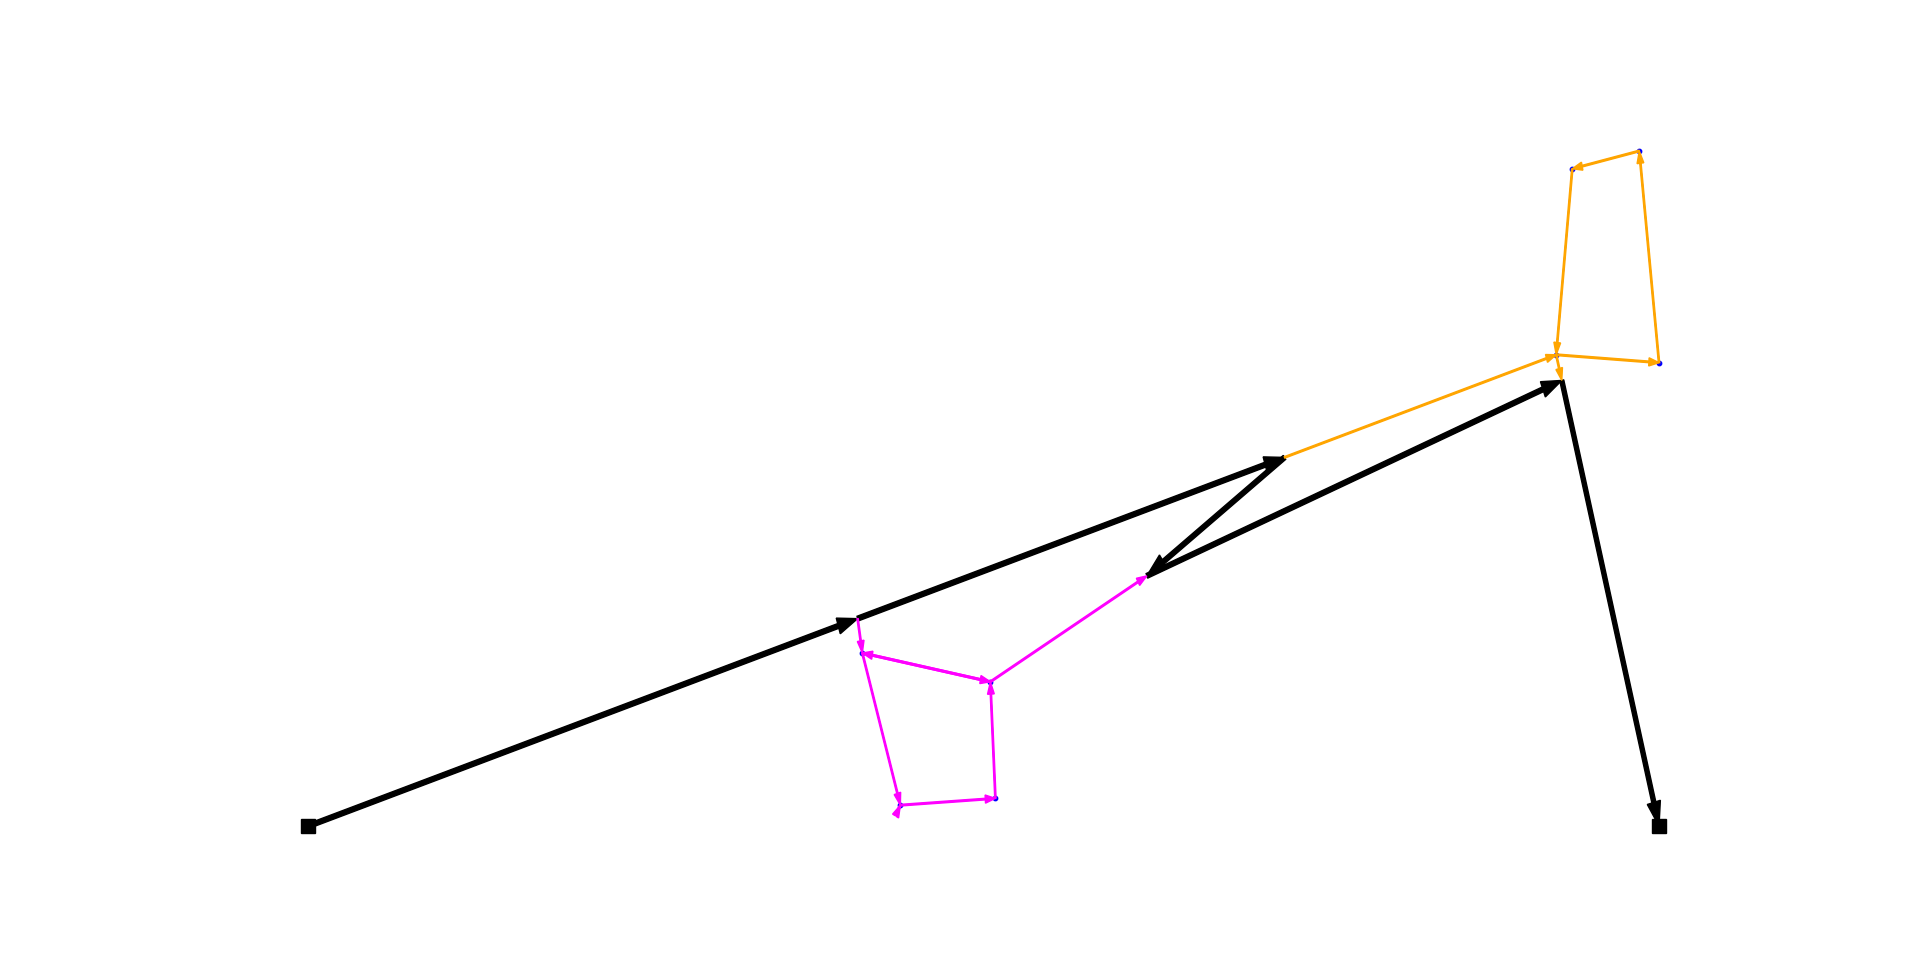
\includegraphics[width=0.6\linewidth]{figures/Asynchronous2-1-46-2.png}
% \end{figure}

\noindent
\RE{To} present our next result, wlog, we restrict ourselves to the degenerate case where graphs reduce to points. \RE{The reader may note that it is possible to reduce the visit of graphs to the visit of points by assuming that the drone is stopped in the point which is at same time that the one required to traverse the edges of the graph. We simplify the proof considering a generic solution between two consecutive target points.}


\begin{theorem}\label{thm:relationship}
Let $x_L^1$, $x_L^2$ (resp. $x_R^1$, $x_R^2$) be the launching (resp. rendezvous) points associated \RE{with} the visit of the target points $P_1$ and $P_2$. If there exist two points $x_L$ and $x_R$ verifying 
$$
 \left\{
 \begin{array}{ccl}
  \dfrac{\|x_L-x_R\|}{v_M} & \leq    & \dfrac{\|x_L - P_1\| + \|P_1 - x_R\|}{v_D}, \\
  \dfrac{\|x_L-x_R\|}{v_M} & \leq    & \dfrac{\|x_L - P_2\| + \|P_2 - x_R\|}{v_D}, \\
  \dfrac{\|x_L-x_R\|}{v_M} & \leq   & N_D, \\
  \|x_L-x_R\| & \leq & \|x_L^1 - x_L^2\| + \|x_L^2- x_R^1\| + \|x_R^1-x_R^2\|,
 \end{array}
 \right.
$$

\noindent then the contribution of this partial route to the optimal objective value will be the same in both models.
\end{theorem}
\begin{figure}[h!]
    \centering
    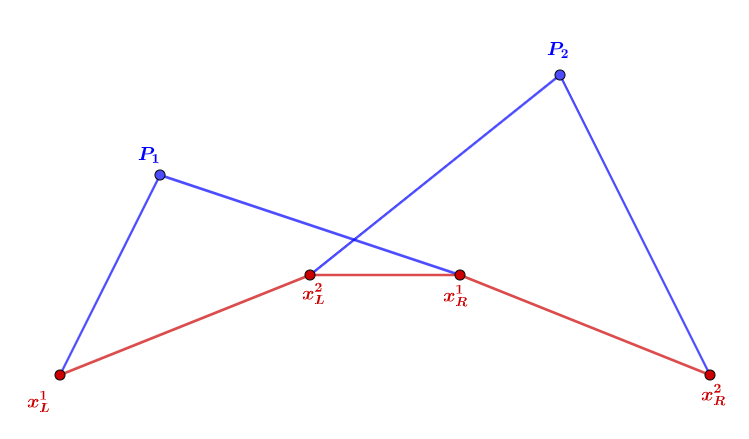
\includegraphics[width = 0.5\linewidth]{proof1.PNG}
    \caption{The mothership launches two drones sequentially}
    \label{fig:proof1}
\end{figure}

\begin{proof}
Note that in the considered configuration, the order of visit\RE{s} to the points $P_1$ and $P_2$ is fixed and then, the binary variables in the model are fixed in this case. Thus, the only difference\RE{s} that the two models can have are the location of the launching and rendezvous points. Hence, the only constraints that are involved are those related to these points. These are the conditions in the statement: The first two are the \eqref{DCW} inequalities. The third one is the \eqref{CAP} constraint and the last one ensures that the distance traveled by the mothership in the \RE{complete overlapping} model is smaller than or equal to the distance assumed in the \RE{partial overlapping} solution described in the statement. Therefore, the conclusion follows.
\end{proof}

\noindent
\RE{Note that this result states sufficient conditions to obtain the same solution for the two models.% \CV{DISCUSS: More implications and meanings?}
}

}
\color{black}
%(Meto restricción de capacidad? para hacer experimentos puede complicarse)

% $$
% e=(i, j) \ni x_R^t \rightarrow V_i \vee V_j \rightarrow \ldots \rightarrow V_k \rightarrow \ldots \rightarrow V_{i'} \rightarrow x_L^{t+1} \in (i',j')=e'
% $$

% The design of these paths obeys to define binary variables that decide which vertices are selected in each stage $t$: 
\section{Mixed Integer Non Linear Programming Formulations}\label{Form}
% \JP{In this section we present a MINLP formulation for the (\AMD). Let us denote by $\mathcal T$ the set of stages/tasks that the mothership and the fleet of drones have to carry out. These stages are visits to the different graphs in $\mathcal G$ with the required constraints. A stage $t\in\mathcal T$ is referred to as the operation in which the mothership launches some drones from a taking-off location, denoted by $x_L^t$ and later it takes them back on a rendezvous location $x_R^t$. Here, it is important to realize that both locations $x^L_t$ and $x^R_t$ must be determined in the continuous space where the mothership is assumed to move. Note that $|\mathcal T|\leq|\mathcal G|$, since it is assumed that, for each stage, at least one drone must be launched. Clearly, the distance $d_{LR}^t$ traveled by the base vehicle for the stage $t$, i.e., to go from $x_L^t$ to $x_R^t$ is
% $$d_{LR}^t=\|x_L^t - x_R^t\|,$$
% where $\|\cdot\|_2$ denoted the Euclidean distance,  although this assumption can be extended to any $l_p$ norm, $1\leq p\leq \infty$.} 
\noindent
In this section\RE{,} we present \RE{a mixed-integer nonlinear programming (MINLP)} formulation for the \AMD\xspace  that can be used to solve medium size instances of this problem.
\noindent
As mentioned in Section \ref{section:desc}, we assume that the mothership is allowed to move freely in a continuous space that for the sake of presentation we  assume to be $\mathbb R^2$. Here, \RE{the} distances are measured by the Euclidean norm, $\|\cdot\|_2$, although this assumption can be extended to any $l_p$ norm, $1\leq p\leq \infty$ (see \cite{Blanco2017}).
\noindent
In the following, we introduce the parameters or input data that formally describe the problem and that are summarized in Table \ref{table:t1}.

 \begin{table}[!h]
\scriptsize
\centering
%\color{blue}
\begin{tabular}{ | l | }
\hline
\textbf{Problem Parameters}\\
\hline
$origin$: coordinates of the point defining the origin of the mothership path (or tour).\\
$dest$: coordinates of the point defining the destination of the mothership path (or tour).\\
$\mathcal{G}$: set of the target graphs.\\
$g = (V_g, E_g)$: set of nodes and edges of each target graph $g \in \mathcal{G}$.\\
$\mathcal{L}(e_g)$: length of edge $e$ of graph $g \in \mathcal{G}$.\\
$\mathcal{L}(g)=\sum_{e_g\in E_g} \mathcal L(e_g)$: total length of the graph $g\in\mathcal G$.\\
$B^{e_g}, C^{e_g}$: coordinates of the endpoints of edge $e$ of graph $g \in \mathcal{G}$.\\
$\alpha^{e_g}$: \RE{fraction of length} of edge $e$ of graph $g \in \mathcal{G}$ that must be visited. \RE{It ranges between 0 and 1.} \\
$\alpha^{g}$: \RE{fraction of length} of graph $g \in \mathcal{G}$ that must be visited. \RE{It ranges between 0 and 1.}\\
$v_M$: mothership speed.\\
\RE{$|\mathcal D|$: \RE{number} of drones.}\\
$v_D$: drone speed.\\
$N_D$: drone endurance. \\
\RE{$\mathcal{O}$: set of drone operations to perform visits to the target graphs. \RE{$\mathcal{O} =\{1,\ldots,|\mathcal{O}|\}$.}  }\\
$M$: big-M constant.\\
\hline
\end{tabular}
\caption{Nomenclature for AMMDRPG-CO}
\label{table:t1}
\end{table}

\begin{table}[h!]
%\tiny
\scriptsize
\centering
%\color{blue}
\begin{tabular}{|l|}
\hline 
\textbf{Binary and Integer Decision Variables}\\
\hline
$\mu^{e_g} \in \{0,1\}, \:\: \forall e_g \in E_g$ ($g \in \mathcal{G}$): equal to 1 if edge $e$ of graph $g$ (or a \RE{fraction} of it) is visited by the drone, 0 otherwise.\\
$\text{entry}^{e_g} \in \{0,1\}, \:\: \forall e_g \in E_g \:\: (g \in \mathcal{G})$: auxiliary binary variable used for linearizing expressions.\\
$u^{e_{g}\RE{o}} \in \{0,1\}, \:\: \forall e_g \in E_g \:\: (g \in \mathcal{G}), \:\: \forall \RE{o} \in \RE{\mathcal O}$: equal to 1 if \RE{one} drone enters in graph $g$ by the edge $e_g$ at \RE{operation $o$}, 0 otherwise.\\
$z^{e_{g}e^{'}_{g}} \in \{0,1\}, \:\: \forall e_g, e_g' \in E_g\:\: (g \in \mathcal{G})$: equal to 1 if \RE{one} drone goes from $e_g$ to $e^{'}_{g}$, 0 otherwise.\\
$v^{e_{g}\RE{o}} \in \{0,1\}, \:\: \forall e_g \in E_g \:\: (g \in \mathcal{G})$, $\: \forall \RE{o} \in \RE{\mathcal O}$: equal to 1 if \RE{one} drone exits from graph $g$ by $e_g$ at \RE{operation $o$}, 0 otherwise.\\
\hline
\textbf{Continuous Decision Variables}\\
\hline
$s^{e_g} \in [0,|E_g|-1], \:\: \forall e_g \in E_g \:\: (g \in \mathcal{G})$: continuous non negative variable representing the order of visit of the edge $e$ of graph $g$.\\
$\rho^{e_g} \in [0,1]$ and $\lambda^{e_g} \in [0,1], \:\: \forall e_g \in E_g \:\: (g \in \mathcal{G})$: defining the entry and exit points on $e_g$.\\
$\nu_\text{min}^{e_g}$ and $\nu_\text{max}^{e_g} \in [0,1], \:\: \forall e_g \in E_g \:\: (g \in \mathcal{G})$: auxiliary variables used for linearizing expressions.\\
$x_L^\RE{o}\in\mathbb R^2, \:\: \forall \RE{o} \in \RE{\mathcal O}$: coordinates representing the point where the mothership launches the drone\RE{s} at \RE{operation $o$}.\\
$x_R^\RE{o}\in\mathbb R^2, \:\: \forall \RE{o} \in \RE{\mathcal O}$: coordinates representing the point where the mothership retrieves the drone\RE{s} at \RE{operation $o$}.\\
$R^{e_g}\in\mathbb R^2, \:\: \forall e_g \in E_g \:\: (g \in \mathcal{G})$: coordinates representing the entry point on edge \RE{$e_g$} of graph $g$.\\
$L^{e_g}\in\mathbb R^2, \:\: \forall e_g \in E_g \:\: (g \in \mathcal{G})$: coordinates representing the exit point on edge \RE{$e_g$} of graph $g$.\\
\CV{$d_{origin}\geq 0$: distance from the origin $origin$ to the first launching point $x_L^1$.}\\
$d_L^{e_g\RE{o}} \geq 0, \:\: \forall e_g \in E_g \:\:(g \in \mathcal{G}), \:\:\forall \RE{o} \in \RE{\mathcal O}$: representing the distance travelled by \RE{one} drone from the launching\\
\hspace*{1cm} point $x_L^\RE{o}$ on the mothership at \RE{operation $o$} to the first visiting point $R^{e_g}$ on $e_g$.\\
\RE{$p_L^{e_g\RE{o}} \geq 0, \:\: \forall e_g \in E_g \:\: (g \in \mathcal{G}), \:\:\forall \RE{o} \in \RE{\mathcal O}$: auxiliary variable used for modelling the product of $d_L^{e_g\RE{o}}$ and $u^{e_g\RE{o}}$.}\\
$d^{e_g} \geq 0, \:\: \forall e_g \in E_g \:\: (g \in \mathcal{G})$: representing the distance travelled by the drone from the rendezvous point $R^{e_g}$ to the \\
\hspace*{1cm} launching point $L^{e_g}$ on $e_g$. \\
\RE{$p^{e_g}\in [0, 1], \:\: \forall e_g \in E_g \:\: (g \in \mathcal G)$: auxiliary variable used for modelling the product of $\mu^{e_g}$ and $|\lambda^{e_g}-\rho^{e_g}|$.}\\
$d^{e_ge^\prime_g} \geq 0, \:\: \forall e_g, e^\prime_g \in E_g \:\:(g \in \mathcal{G})$: representing the distance travelled by the drone from the launching point $L^{e_g}$ on $e_g$ to\\
\hspace*{1cm}  the rendezvous point $R^{e^\prime_g}$ on $e^\prime_g$.\\
\RE{$p^{e_ge^\prime_g} \geq 0, \:\: \forall e_g, e^\prime_g \in E_g \:\:(g \in \mathcal{G})$: auxiliary variable used for modelling the product of $d^{e_ge^\prime_g}$ and $z^{e_ge^\prime_g}$.}\\
$d_R^{e_g\RE{o}} \geq 0, \:\: \forall e_g \in E_g \:\:(g \in \mathcal{G}), \:\:\forall \RE{o} \in \RE{\mathcal O}$: representing the distance travelled by \RE{one} drone from the last visiting point\\
\hspace*{1cm} $L^{e_g}$ on $e_g$ to the rendezvous point $x_R^\RE{o}$ on the mothership at \RE{operation $o$}.\\
\RE{$p_R^{e_g\RE{o}} \geq 0, \:\: \forall e_g \in E_g \:\:(g \in \mathcal{G}), \:\:\forall \RE{o} \in \RE{\mathcal O}$: auxiliary variable used for modelling the product of $d_R^{e_g\RE{o}}$ and $v^{e_g\RE{o}}$.}\\
$d_{LR}^\RE{o} \geq 0, \:\: \forall \RE{o} \in \RE{\mathcal O}$: representing the distance travelled by the mothership from the launching point $x_L^\RE{o}$ to the rendezvous\\
\hspace*{1cm}   point $x_R^\RE{o}$ at \RE{operation $o$}.\\
$d_{RL}^\RE{o} \geq 0, \:\: \forall \RE{o} \in \RE{\mathcal O}\RE{\setminus |\mathcal O|}$: representing the distance travelled by the mothership from the rendezvous point $x_R^\RE{o}$ at \RE{operation $o$} to the \\ 
\hspace*{1cm}  launching point $x_L^{(\RE{o}+1)}$ at \RE{operation $o+1$}.\\
\CV{$d_{dest}\geq 0$: distance from the last retrieving point $x_R^{|\mathcal O|}$ to the destination $dest$.}\\
\RE{
$time_D^o \geq 0, \:\: \forall o \in \mathcal O$: maximum time spent by a drone during operation $o$}.\\
\RE{$time_M^o \geq 0, \:\: \forall o \in \mathcal O$: time spent by the mothership to go from the launching point $x_L^o$ to the retrieving point $x_R^o$ of operation $o$.}\\
\RE{$time_M \geq 0$: total time spent by the mothership to go from the origin to the destination.}\\
\hline
\end{tabular}
\caption{Decision Variables for AMMDRPG-CO}
\label{table:t2}
\end{table}

\noindent
\JP{In the following, we describe all the constraints required to formulate the \AMD\xspace model}. Table \ref{table:t2} summarizes the set of decision variables that appear in that formulation.
\subsection*{Visits of graphs}
\noindent
To represent the movement of the drone within a graph $g\in\mathcal G$, we proceed to introduce some notation related to $g$.
Let $g = (V_g, E_g)$ be a graph in $\mathcal G$ whose total length is denoted by $\mathcal L(g)$. Here, $V_g$ denotes the set of nodes and $E_g$ denotes the set of edges connecting pairs of nodes.  Let $e_g$ be \RE{the} edge $e$ of the graph $g \in G$ and let $\mathcal  L(e_g)$ be its length. Each edge $e_g$ is parameterized by its endpoints $B^{e_g}= (B^{e_g}(x_1), B^{e_g}(x_2))$ and $C^{e_g}= (C^{e_g}(x_1), C^{e_g}(x_2))$ and we can compute its length $\mathcal L(e_g) =\|C^{e_g} -  B^{e_g}\|$. 

\noindent
\RE{For each edge $e_g$ it is associated an indicator binary variable $\mu^{e_g}$ that is one if the drone visits the segment $e_g$. Moreover, we define the entry and exit points $R^{e_g}=(B^{e_g},C^{e_g},\rho^{e_g})$ and $L^{e_g}=(B^{e_g},C^{e_g},\lambda^{e_g})$ \RE{that determine the fraction of the edge visited by the drone}. The coordinates of the points $R^{e_g}$ and $L^{e_g}$ are given, respectively by 
$$R^{e_g} = \rho^{e_g} B^{e_g} + (1- \rho^{e_g})C^{e_g} \quad\text{ and }\quad L^{e_g} = \lambda^{e_g} B^{e_g} + (1- \lambda^{e_g})C^{e_g},$$ where $\rho^{e_g} \in [0,1]$ and $\lambda^{e_g} \in [0,1]$ are variables to determine the position of the points on the segment.}



\noindent
As discussed in Section \ref{section:desc}, we consider two modes of visit to the target graphs $g\in \mathcal{G}$:
\begin{itemize}
    \item Visiting a \RE{fraction} $\alpha^{e_g}$ of each edge $e_g$ which can be modeled by using the following constraints:
    \begin{equation}\label{eq:alphaE}\tag{$\alpha$-E}
    |\lambda^{e_g} - \rho^{e_g}|\geq \alpha^{e_g}, \quad \forall e_g\in E_g.
    \end{equation}
    \RE{These inequalities state that the difference between the parameterizations of the entry and exit points associated to each edge $e_g$ must be higher than the fraction of the length of $e_g$ required to be traversed.}
    \item Visiting a \RE{fraction} $\alpha^g$ of the total length of the graph:
    \begin{equation}\label{eq:alphaG}\tag{$\alpha$-G}
    \sum_{e_g\in E_g} \mu^{e_g}|\lambda^{e_g} - \rho^{e_g}|\mathcal L(e_g) \geq \alpha^g\mathcal L(g).
    \end{equation}
    \RE{This constraint ensures that the sum of the fractions of length of those edges chosen to be crossed must be higher than the fraction of length of $g$ required to be traversed.}
   % \CV{where $\mathcal L(g)$ denotes the total length of the graph., this is mentioned before}
\end{itemize}



\bigskip
\noindent
In both cases\RE{,} the corresponding constraints are nonlinear. \RE{To} linearize them, we need to introduce a binary variable $\text{entry}^{e_g}$ that determines the traveling direction on the edge $e_g$ as well as the definition of the \RE{auxiliary variables} $\nu_\text{min}^{e_g}$ and $\nu_\text{max}^{e_g}$ of the access and exit points \RE{on} that segment. Then, for each edge $e_g$, the absolute value constraint \eqref{eq:alphaE} can be represented by:

\begin{equation}\label{eq:alpha-E}\tag{$\alpha$-E}
 |\rho^{e_g}-\lambda^{e_g}|\geq \alpha^{e_g} \Longleftrightarrow
 \left\{
 \begin{array}{ccl}
  \rho^{e_g} - \lambda^{e_g}                       & =    & \nu_\text{max}^{e_g} - \nu_\text{min}^{e_g},                                     \\
  \nu_\text{max}^{e_g}                         & \leq & 1-{\text{entry}^{e_g}},                                   \\
  \nu_\text{min}^{e_g}                      & \leq & {  \text{entry}^{e_g}},                                        \\
    \nu_\text{min}^{e_g}, \,\nu_\text{max}^{e_g} & \geq & 0, \\

  \nu_\text{max}^{e_g} + \nu_\text{min}^{e_g} & \geq & \alpha^{e_g}.
  \\
 \end{array}
 \right.
\end{equation}
The first four inequalities model the standard trick of the linearization of the absolute value. The last constraint ensures that the value of the linear expression of the absolute value is higher than the required \RE{fraction} $\alpha^{e_g}$.
\noindent
Similarly, \eqref{eq:alphaG} can be linearized as follows:
\begin{equation}\label{eq:alpha-G}\tag{$\alpha$-G}
 \sum_{e_g\in E_g} \mu^{e_g}|\rho^{e_g}-\lambda^{e_g}|\mathcal L(e_g)\geq \alpha^g\mathcal L(g). \Longleftrightarrow
 \left\{
 \begin{array}{ccl}
  \rho^{e_g} - \lambda^{e_g}                       & =    & \nu_\text{max}^{e_g} - \nu_\text{min}^{e_g},                                     \\
  \nu_\text{max}^{e_g}                         & \leq & 1-{\text{entry}^{e_g}},                                   \\
  \nu_\text{min}^{e_g}                      & \leq & {  \text{entry}^{e_g}},                                        \\
  \nu_\text{min}^{e_g}, \,\nu_\text{max}^{e_g} & \geq & 0, \\
  p^{e_g} & \leq & \nu_\text{max}^{e_g} + \nu_\text{min}^{e_g}, \\
  p^{e_g} & \leq & \mu^{e_g}, \\
  p^{e_g} & \geq & \nu_\text{max}^{e_g} + \nu_\text{min}^{e_g} + \mu^{e_g} - 1, \\
  \sum_{e_g\in E_g} p^{e_g}\mathcal L(e_g) & \geq & \alpha^{g}\mathcal L(g),
  \\
 \end{array}
 \right.
\end{equation}
where $p^{e_g}$ is the auxiliary variable that represents the product of the binary variable $\mu^{e_g}$ and the absolute value difference $|\rho^{e_g} - \lambda^{e_g}|$. The first four inequalities linearize \RE{again the absolute value} expression. The \RE{following} three constraints model the product of the expression of the absolute value and the binary variable $\mu^{e_g}$. The last inequality ensures that the fraction of the length of those edges chosen to be crossed must be higher than the fraction of the length of $g$ required to be traversed.
%}

\subsection*{Elimination of subtours}
\noindent
\RE{To} represent \RE{the} actual routes of the drones over the target graph, subtours cannot be allowed. \RE{The reader may note that the subtour elimination constraints are needed to avoid the presence of disconnected paths on the edges of the graph.} To prevent the existence of subtours within each graph $g\in \mathcal G$ that the drone must visit, one can include, among others, either the compact formulation that uses the Miller-Tucker-Zemlin constraints (MTZ) or the subtour elimination constraints (SEC).\\
\noindent
For the MTZ formulation, we use the continuous variables $s^{e_g}$, defined in Table \ref{table:t2}, that state the order to visit the edge $e_g$ and set the following constraints for each $g\in\mathcal G$:

\begin{align}
    s^{e_g} - s^{e^\prime_g} + |E_g|z^{e_ge^\prime_g} & \leq |E_g| - 1  , &\quad\forall e_g \neq e_g'\in E_g, \tag{MTZ$_1$} \label{MTZ1}\\
    0 & \leq s^{e_g} \leq |E_g| - 1, &\quad\forall e_g\in E_g.\tag{MTZ$_2$}\label{MTZ2}
\end{align}

\noindent
Alternatively, we can also use the family of subtour elimination constraints for each $g\in\mathcal G$:
\begin{equation}\tag{SEC}\label{SEC}
    \sum_{e_g, e^\prime_g \in S} z_g^{e_ge^\prime_g} \leq |S| - 1, \quad \forall S\subset E_g.
\end{equation}

\noindent
%(Copiado del XPPN)
Since there is an exponential number of SEC constraints, when we implement this formulation\RE{,} we need to perform a row generation procedure including constraints whenever they are required by a separation oracle. To find SEC inequalities, as usual, we search for disconnected components in the current solution. Among them, we choose the shortest subtour found in the solution to be added as a lazy constraint to the model.\\

%\CV{Maybe we should include a sentence to introduce the subsections and clarifying that the previous ones are common in both models}
\subsection{\AMD\xspace  with complete overlapping} \label{subsec:CO}
\noindent
To model this problem, we use \RE{operations} identified with the order in which the different \RE{target graphs} in the problem are visited. Let us denote by $\mathcal O$ the set of \RE{operations} that the mothership and the fleet of drones have to carry out. These \RE{operations} are visits to different graphs in $\mathcal G$ with the required constraints. \RE{An \textit{operation} $o\in\mathcal O$} is referred to as the \RE{actions} in which the mothership launches some drones from a taking-off location, denoted by $x_L^o$ and later it takes them back on a rendezvous location $x_R^o$. Here, it is important to realize that both locations $x_L^o$ and $x_R^o$ must be determined in the continuous space where the mothership is assumed to move. Note that $|\mathcal O|\leq|\mathcal G|$, since it is assumed that, for each operation, at least one drone must be launched.
\noindent
For each operation $o\in\mathcal O$, each one of the drones launched from the mothership must follow a path starting from and returning to the mothership, while visiting the required edges of \LA{one of the graph $g \in \mathcal G$}. According to the notation introduced above, we write this generic path in the following form:

$$
x_L^o\rightarrow R^{e_g}\rightarrow L^{e_g}\rightarrow\ldots\rightarrow R^{e^\prime_g}\rightarrow L^{e^\prime_g}\rightarrow \ldots \rightarrow R^{e''_g}  \rightarrow L^{e''_g} \rightarrow x_R^o. %\RE{R1.18: \sout{\rightarrow x_L^{t+1}}}.
$$


% \begin{figure}[h!]
% \centering
% 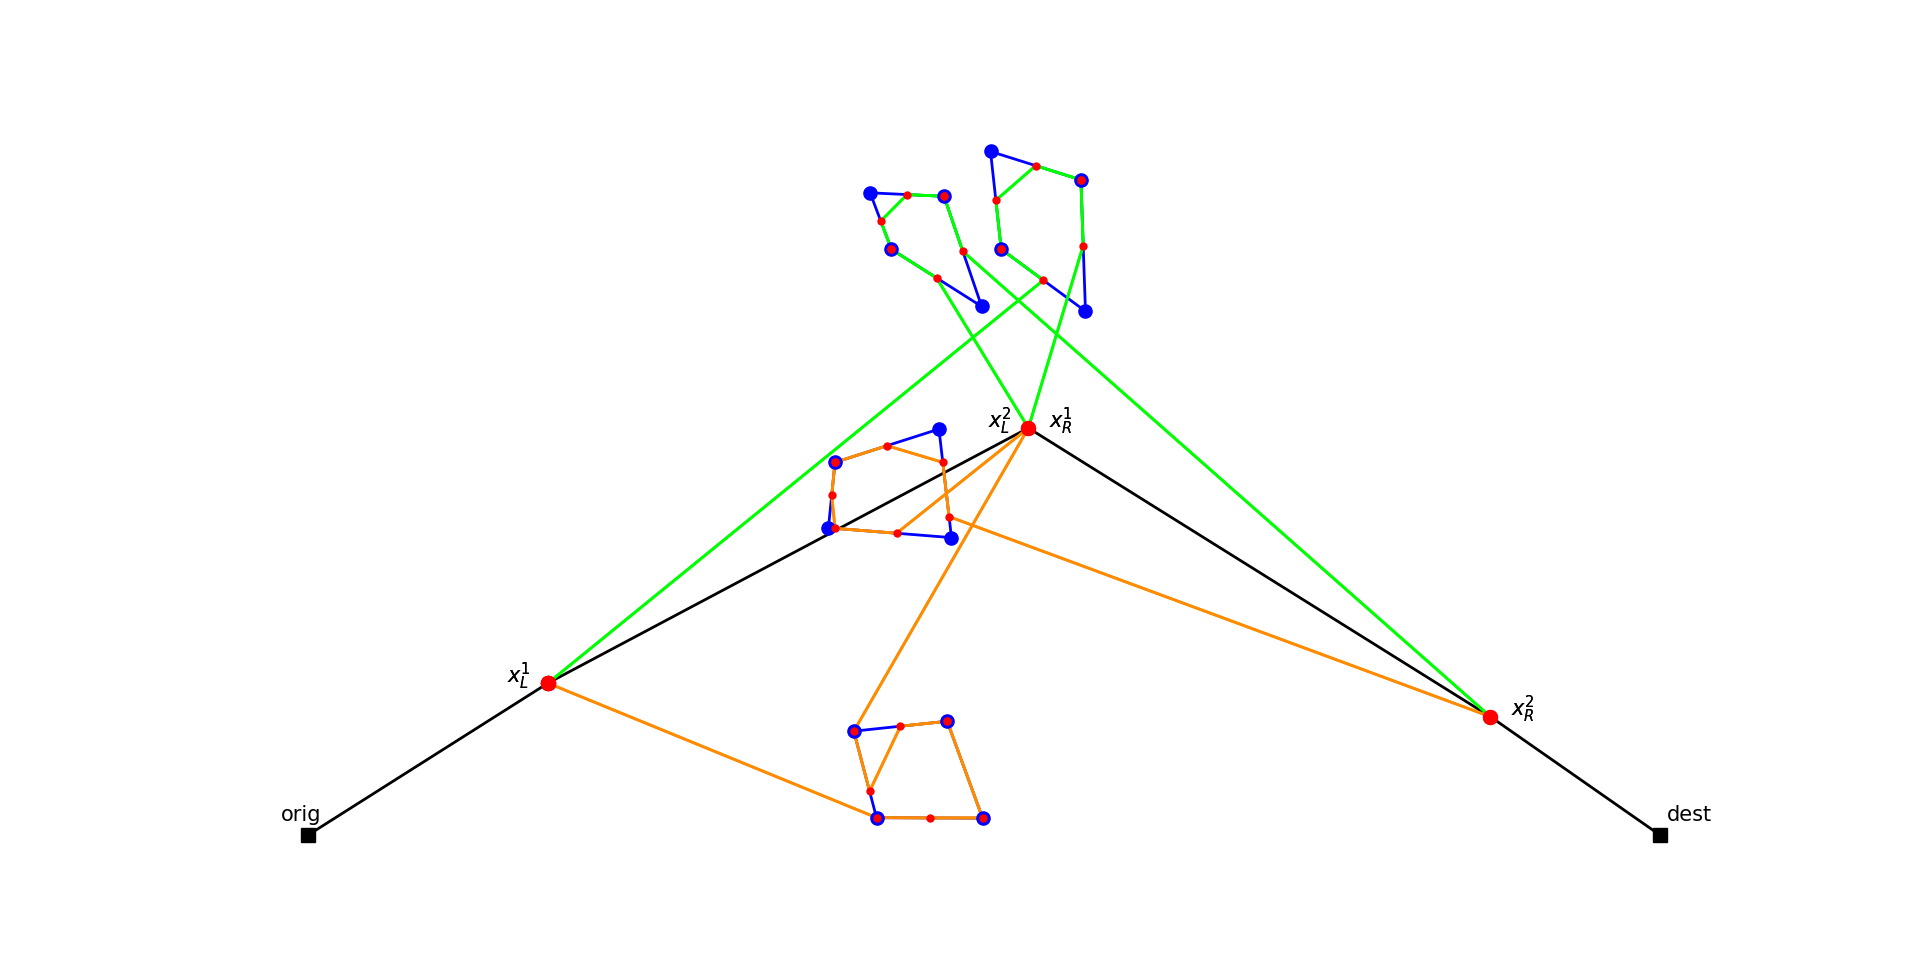
\includegraphics[width=0.95\linewidth]{figures/figure_latex.png}
% \caption{Example illustrating the meaning of the launching  (L) and retrieving (R) points.}
% \label{fig:illustrative}
% \end{figure}

%% This file was created with tikzplotlib v0.9.12.
\begin{figure}[h!]
\centering
% This file was created with tikzplotlib v0.9.12.
\begin{tikzpicture}

\definecolor{color0}{rgb}{1,0.549019607843137,0}

\begin{axis}[
hide x axis,
hide y axis,
scaled x ticks=manual:{}{\pgfmathparse{#1}},
scaled y ticks=manual:{}{\pgfmathparse{#1}},
tick align=outside,
x grid style={white!69.0196078431373!black},
xmajorticks=false,
xmin=-5, xmax=105,
xtick style={color=black},
xticklabels={},
y grid style={white!69.0196078431373!black},
ymajorticks=false,
ymin=-5, ymax=75,
ytick style={color=black},
yticklabels={}
]
\path [draw=blue, thick]
(axis cs:21.0696182692914,1.38670279952717)
--(axis cs:30.306045132353,1.50447958089156);

\path [draw=blue, thick]
(axis cs:21.0696182692914,1.38670279952717)
--(axis cs:23.9355243392435,8.22107815581281);

\path [draw=blue, thick]
(axis cs:30.306045132353,1.50447958089156)
--(axis cs:30.6007400849981,8.61180925900065);

\path [draw=blue, thick]
(axis cs:23.9355243392435,8.22107815581281)
--(axis cs:30.6007400849981,8.61180925900065);

\path [draw=blue, thick]
(axis cs:4.08370396767994,62.5193171258523)
--(axis cs:8.09069545603466,60.4417973648425);

\path [draw=blue, thick]
(axis cs:4.08370396767994,62.5193171258523)
--(axis cs:2.37426610997379,66.9905560181573);

\path [draw=blue, thick]
(axis cs:8.09069545603466,60.4417973648425)
--(axis cs:8.40433589338944,70.7975020391092);

\path [draw=blue, thick]
(axis cs:2.37426610997379,66.9905560181573)
--(axis cs:8.40433589338944,70.7975020391092);

\path [draw=blue, thick]
(axis cs:21.0664581490033,38.3255279820558)
--(axis cs:29.0472438012912,42.369596955967);

\path [draw=blue, thick]
(axis cs:21.0664581490033,38.3255279820558)
--(axis cs:22.1750046919912,47.5858849832036);

\path [draw=blue, thick]
(axis cs:29.0472438012912,42.369596955967)
--(axis cs:27.0356718607916,49.5164362980235);

\path [draw=blue, thick]
(axis cs:22.1750046919912,47.5858849832036)
--(axis cs:27.0356718607916,49.5164362980235);

\path [draw=blue, thick]
(axis cs:89.6170857784204,29.8130206242151)
--(axis cs:98.4204942730176,31.9280359170996);

\path [draw=blue, thick]
(axis cs:89.6170857784204,29.8130206242151)
--(axis cs:89.5168058385155,39.6742972814671);

\path [draw=blue, thick]
(axis cs:98.4204942730176,31.9280359170996)
--(axis cs:97.2556927544101,39.0446066906692);

\path [draw=blue, thick]
(axis cs:89.5168058385155,39.6742972814671)
--(axis cs:97.2556927544101,39.0446066906692);

\path [draw=black, thick]
(axis cs:0,0)
--(axis cs:0,0)
--(axis cs:11.9384375817266,38.1768740390765)
--(axis cs:10.3131414759248,47.5858849832036)
--(axis cs:44.9451427093311,40.8090894507933)
--(axis cs:64.0827735142413,29.8198845110857)
--(axis cs:95.4029040306271,4.93918065109767)
--(axis cs:100,0);
\path [draw=green, thick]
(axis cs:0,0)
--(axis cs:21.0696182692914,1.38670279952717)
--(axis cs:25.6878317008222,1.44559119020937)
--(axis cs:30.3792241725836,3.26938108252212)
--(axis cs:30.5265716489061,6.82304592157666)
--(axis cs:27.2681322121208,8.41644370740673)
--(axis cs:23.9355243392435,8.22107815581281)
--(axis cs:23.9355243392435,8.22107815581281)
--(axis cs:22.5025713042674,4.80389047767)
--(axis cs:11.9384375817266,38.1768740390765);
\path [draw=color0, thick]
(axis cs:0,0)
--(axis cs:21.0664581490033,38.3255279820558)
--(axis cs:25.0568509751472,40.3475624690114)
--(axis cs:29.0472438012912,42.369596955967)
--(axis cs:28.0414578310414,45.9430166269952)
--(axis cs:24.6053382763914,48.5511606406136)
--(axis cs:22.1750046919912,47.5858849832036)
--(axis cs:22.1750046919912,47.5858849832036)
--(axis cs:21.3637623976544,40.8090894507933)
--(axis cs:11.9384375817266,38.1768740390765);
\path [draw=green, thick]
(axis cs:0,0)
--(axis cs:21.0696182692914,1.38670279952717)
--(axis cs:25.6878317008222,1.44559119020937)
--(axis cs:30.3792241725836,3.26938108252212)
--(axis cs:30.5265716489061,6.82304592157666)
--(axis cs:27.2681322121208,8.41644370740673)
--(axis cs:23.9355243392435,8.22107815581281)
--(axis cs:23.9355243392435,8.22107815581281)
--(axis cs:22.5025713042674,4.80389047767)
--(axis cs:11.9384375817266,38.1768740390765);
\path [draw=color0, thick]
(axis cs:0,0)
--(axis cs:21.0664581490033,38.3255279820558)
--(axis cs:25.0568509751472,40.3475624690114)
--(axis cs:29.0472438012912,42.369596955967)
--(axis cs:28.0414578310414,45.9430166269952)
--(axis cs:24.6053382763914,48.5511606406136)
--(axis cs:22.1750046919912,47.5858849832036)
--(axis cs:22.1750046919912,47.5858849832036)
--(axis cs:21.3637623976544,40.8090894507933)
--(axis cs:11.9384375817266,38.1768740390765);
\path [draw=green, thick]
(axis cs:10.3131414759248,47.5858849832036)
--(axis cs:8.09069545603467,60.4417973648425)
--(axis cs:6.08719971185731,61.4805572453474)
--(axis cs:8.1475539671049,62.3191380350312)
--(axis cs:8.30437418578229,67.4969903721645)
--(axis cs:5.38930100168162,68.8940290286332)
--(axis cs:2.37426610997379,66.9905560181573)
--(axis cs:2.3742661099738,66.9905560181572)
--(axis cs:3.22898503882687,64.7549365720048)
--(axis cs:44.9451427093311,40.8090894507933);
\path [draw=green, thick]
(axis cs:10.3131414759248,47.5858849832036)
--(axis cs:8.09069545603467,60.4417973648425)
--(axis cs:6.08719971185731,61.4805572453474)
--(axis cs:8.1475539671049,62.3191380350312)
--(axis cs:8.30437418578229,67.4969903721645)
--(axis cs:5.38930100168162,68.8940290286332)
--(axis cs:2.37426610997379,66.9905560181573)
--(axis cs:2.3742661099738,66.9905560181572)
--(axis cs:3.22898503882687,64.7549365720048)
--(axis cs:44.9451427093311,40.8090894507933);
\path [draw=green, thick]
(axis cs:64.0827735142413,29.8198845110857)
--(axis cs:89.6170857784204,29.8130206242151)
--(axis cs:94.018790025719,30.8705282706573)
--(axis cs:97.8380935137139,35.4863213038844)
--(axis cs:97.2556927544101,39.0446066906692)
--(axis cs:97.25569275441,39.0446066906692)
--(axis cs:93.3862492964628,39.3594519860681)
--(axis cs:89.5669458084679,34.7436589528409)
--(axis cs:89.6170857784204,29.8130206242149)
--(axis cs:95.4029040306271,4.93918065109767);
\path [draw=green, thick]
(axis cs:64.0827735142413,29.8198845110857)
--(axis cs:89.6170857784204,29.8130206242151)
--(axis cs:94.018790025719,30.8705282706573)
--(axis cs:97.8380935137139,35.4863213038844)
--(axis cs:97.2556927544101,39.0446066906692)
--(axis cs:97.25569275441,39.0446066906692)
--(axis cs:93.3862492964628,39.3594519860681)
--(axis cs:89.5669458084679,34.7436589528409)
--(axis cs:89.6170857784204,29.8130206242149)
--(axis cs:95.4029040306271,4.93918065109767);
\addplot [draw=blue, fill=blue, mark=*, only marks]
table{%
x  y
21.0696182692914 1.38670279952717
30.306045132353 1.50447958089156
23.9355243392435 8.22107815581281
30.6007400849981 8.61180925900065
};
\addplot [draw=blue, fill=blue, mark=*, only marks]
table{%
x  y
4.08370396767994 62.5193171258523
8.09069545603466 60.4417973648425
2.37426610997379 66.9905560181573
8.40433589338944 70.7975020391092
};
\addplot [draw=blue, fill=blue, mark=*, only marks]
table{%
x  y
21.0664581490033 38.3255279820558
29.0472438012912 42.369596955967
22.1750046919912 47.5858849832036
27.0356718607916 49.5164362980235
};
\addplot [draw=blue, fill=blue, mark=*, only marks]
table{%
x  y
89.6170857784204 29.8130206242151
98.4204942730176 31.9280359170996
89.5168058385155 39.6742972814671
97.2556927544101 39.0446066906692
};
\addplot [semithick, red, mark=*, mark size=1, mark options={solid}, only marks]
table {%
25.6878317008222 1.44559119020937
21.0696182692914 1.38670279952717
23.9355243392435 8.22107815581281
22.5025713042674 4.80389047767
30.3792241725836 3.26938108252212
30.5265716489061 6.82304592157666
27.2681322121208 8.41644370740673
23.9355243392435 8.22107815581281
8.09069545603467 60.4417973648425
6.08719971185731 61.4805572453474
2.3742661099738 66.9905560181572
3.22898503882687 64.7549365720048
8.1475539671049 62.3191380350312
8.30437418578229 67.4969903721645
5.38930100168162 68.8940290286332
2.37426610997379 66.9905560181573
21.0664581490033 38.3255279820558
25.0568509751472 40.3475624690114
22.1750046919912 47.5858849832036
21.3637623976544 40.8090894507933
29.0472438012912 42.369596955967
28.0414578310414 45.9430166269952
24.6053382763914 48.5511606406136
22.1750046919912 47.5858849832036
89.6170857784204 29.8130206242151
94.018790025719 30.8705282706573
89.5669458084679 34.7436589528409
89.6170857784204 29.8130206242149
97.8380935137139 35.4863213038844
97.2556927544101 39.0446066906692
97.25569275441 39.0446066906692
93.3862492964628 39.3594519860681
};
\addplot [semithick, black, opacity=1, mark=square*, mark size=2.5, mark options={solid}, only marks]
table {%
0 0
100 0
};
\addplot [semithick, red, opacity=1, mark=*, mark size=1.5, mark options={solid}, only marks]
table {%
0 0
11.9384375817266 38.1768740390765
10.313141475924828 47.585884983203592
44.9451427093311 40.8090894507933
64.082773514241339 29.819884511085665
95.4029040306271 4.93918065109767
};
\draw (0,10) node[
  scale=0.75,
  anchor=base west,
  text=black,
  rotate=0.0
]{origin};
\draw (0,10) node[
  scale=0.75,
  anchor=base west,
  text=black,
  rotate=0.0
]{origin};
\draw (axis cs:3.4384375817266,38.1768740390765) node[
  scale=0.75,
  anchor=base west,
  text=black,
  rotate=0.0
]{$x_R^1$};
\draw (axis cs:2,3) node[
  scale=0.75,
  anchor=base west,
  text=black,
  rotate=0.0
]{$x_L^1$};
\draw (axis cs:3.4384375817266,38.1768740390765) node[
  scale=0.75,
  anchor=base west,
  text=black,
  rotate=0.0
]{$x_R^1$};
\draw (axis cs:2,3) node[
  scale=0.75,
  anchor=base west,
  text=black,
  rotate=0.0
]{$x_L^1$};
\draw (axis cs:46.4451427093311,40.8090894507933) node[
  scale=0.75,
  anchor=base west,
  text=black,
  rotate=0.0
]{$x_R^2$};
\draw (axis cs:2.7,47.5858849832036) node[
  scale=0.75,
  anchor=base west,
  text=black,
  rotate=0.0
]{$x_L^2$};
\draw (axis cs:46.4451427093311,40.8090894507933) node[
  scale=0.75,
  anchor=base west,
  text=black,
  rotate=0.0
]{$x_R^2$};
\draw (axis cs:2.7,47.5858849832036) node[
  scale=0.75,
  anchor=base west,
  text=black,
  rotate=0.0
]{$x_L^2$};
\draw (axis cs:86,1) node[
  scale=0.75,
  anchor=base west,
  text=black,
  rotate=0.0
]{$x_R^3$};
\draw (axis cs:55.0827735142413,27) node[
  scale=0.75,
  anchor=base west,
  text=black,
  rotate=0.0
]{$x_L^3$};
\draw (axis cs:86,1) node[
  scale=0.75,
  anchor=base west,
  text=black,
  rotate=0.0
]{$x_R^3$};
\draw (axis cs:55.0827735142413,27) node[
  scale=0.75,
  anchor=base west,
  text=black,
  rotate=0.0
]{$x_L^3$};
\draw (100, 10) node[
  scale=0.75,
  anchor=base west,
  text=black,
  rotate=0.0
]{dest};
\draw (100, 10) node[
  scale=0.75,
  anchor=base west,
  text=black,
  rotate=0.0
]{dest};
\end{axis}
\end{tikzpicture}
\subcaption{[a]}
\begin{tikzpicture}
\definecolor{color0}{rgb}{1,0.549019607843137,0}
\begin{axis}[
hide x axis,
hide y axis,
scaled x ticks=manual:{}{\pgfmathparse{#1}},
scaled y ticks=manual:{}{\pgfmathparse{#1}},
tick align=outside,
x grid style={white!69.0196078431373!black},
xmajorticks=false,
xmin=-5, xmax=105,
xtick style={color=black},
xticklabels={},
y grid style={white!69.0196078431373!black},
ymajorticks=false,
ymin=-5, ymax=75,
ytick style={color=black},
yticklabels={}
]
\path [draw=blue, thick]
(axis cs:21.0696182692914,1.38670279952717)
--(axis cs:30.306045132353,1.50447958089156);

\path [draw=blue, thick]
(axis cs:21.0696182692914,1.38670279952717)
--(axis cs:23.9355243392435,8.22107815581281);

\path [draw=blue, thick]
(axis cs:30.306045132353,1.50447958089156)
--(axis cs:30.6007400849981,8.61180925900065);

\path [draw=blue, thick]
(axis cs:23.9355243392435,8.22107815581281)
--(axis cs:30.6007400849981,8.61180925900065);

\path [draw=blue, thick]
(axis cs:4.08370396767994,62.5193171258523)
--(axis cs:8.09069545603466,60.4417973648425);

\path [draw=blue, thick]
(axis cs:4.08370396767994,62.5193171258523)
--(axis cs:2.37426610997379,66.9905560181573);

\path [draw=blue, thick]
(axis cs:8.09069545603466,60.4417973648425)
--(axis cs:8.40433589338944,70.7975020391092);

\path [draw=blue, thick]
(axis cs:2.37426610997379,66.9905560181573)
--(axis cs:8.40433589338944,70.7975020391092);

\path [draw=blue, thick]
(axis cs:21.0664581490033,38.3255279820558)
--(axis cs:29.0472438012912,42.369596955967);

\path [draw=blue, thick]
(axis cs:21.0664581490033,38.3255279820558)
--(axis cs:22.1750046919912,47.5858849832036);

\path [draw=blue, thick]
(axis cs:29.0472438012912,42.369596955967)
--(axis cs:27.0356718607916,49.5164362980235);

\path [draw=blue, thick]
(axis cs:22.1750046919912,47.5858849832036)
--(axis cs:27.0356718607916,49.5164362980235);

\path [draw=blue, thick]
(axis cs:89.6170857784204,29.8130206242151)
--(axis cs:98.4204942730176,31.9280359170996);

\path [draw=blue, thick]
(axis cs:89.6170857784204,29.8130206242151)
--(axis cs:89.5168058385155,39.6742972814671);

\path [draw=blue, thick]
(axis cs:98.4204942730176,31.9280359170996)
--(axis cs:97.2556927544101,39.0446066906692);

\path [draw=blue, thick]
(axis cs:89.5168058385155,39.6742972814671)
--(axis cs:97.2556927544101,39.0446066906692);

\path [draw=black, thick]
(axis cs:0,0)
--(axis cs:5.19517108668237e-05,5.19721988422751e-05)
--(axis cs:8.31804668177588,39.1256215879103)
--(axis cs:8.0902667404291,41.3992381927182)
--(axis cs:41.9928361091472,39.3784823234059)
--(axis cs:61.5718673452208,26.0879192386296)
--(axis cs:94.5456634712005,3.70413789044963)
--(axis cs:100,0);
\path [draw=green, thick]
(axis cs:5.19517108668237e-05,5.19721988422751e-05)
--(axis cs:21.0696185355958,1.3867034345879)
--(axis cs:22.5025656416375,4.80387697389931)
--(axis cs:24.9379489929542,1.43602918392242)
--(axis cs:29.5561397992636,1.49491728610282)
--(axis cs:30.353931133669,2.65937414309857)
--(axis cs:30.5012780269027,6.21302491945877)
--(axis cs:29.1826401424249,8.52867680295897)
--(axis cs:25.850065249296,8.33331318471784)
--(axis cs:8.31804668177588,39.1256215879103);
\path [draw=green, thick]
(axis cs:5.19517108668237e-05,5.19721988422751e-05)
--(axis cs:21.0696185355958,1.3867034345879)
--(axis cs:22.5025656416375,4.80387697389931)
--(axis cs:24.9379489929542,1.43602918392242)
--(axis cs:29.5561397992636,1.49491728610282)
--(axis cs:30.353931133669,2.65937414309857)
--(axis cs:30.5012780269027,6.21302491945877)
--(axis cs:29.1826401424249,8.52867680295897)
--(axis cs:25.850065249296,8.33331318471784)
--(axis cs:8.31804668177588,39.1256215879103);
\path [draw=green, thick]
(axis cs:8.0902667404291,41.3992381927182)
--(axis cs:6.08717590107675,61.4805695906112)
--(axis cs:4.0837005407278,62.5193189026369)
--(axis cs:4.08369465698464,62.5193414790879)
--(axis cs:3.22897670117108,64.7549583801393)
--(axis cs:2.84174575638185,67.2856885528858)
--(axis cs:5.85674978390742,69.1891420779693)
--(axis cs:8.3052804744899,67.5269139951667)
--(axis cs:8.14846106263484,62.3490882974996)
--(axis cs:41.9928361091472,39.3784823234059);
\path [draw=color0, thick]
(axis cs:8.0902667404291,41.3992381927182)
--(axis cs:27.6728191506586,47.2527393224256)
--(axis cs:28.7000788954416,43.6030262742796)
--(axis cs:24.4315739690114,40.0307185577996)
--(axis cs:28.4696719165738,42.0769264544708)
--(axis cs:22.0922910532811,46.8949281369037)
--(axis cs:21.5323008920902,42.2169930131509)
--(axis cs:23.3011399504012,48.0331614224841)
--(axis cs:25.830886920397,49.0379219151249)
--(axis cs:41.9928361091472,39.3784823234059);
\path [draw=green, thick]
(axis cs:8.0902667404291,41.3992381927182)
--(axis cs:6.08717590107675,61.4805695906112)
--(axis cs:4.0837005407278,62.5193189026369)
--(axis cs:4.08369465698464,62.5193414790879)
--(axis cs:3.22897670117108,64.7549583801393)
--(axis cs:2.84174575638185,67.2856885528858)
--(axis cs:5.85674978390742,69.1891420779693)
--(axis cs:8.3052804744899,67.5269139951667)
--(axis cs:8.14846106263484,62.3490882974996)
--(axis cs:41.9928361091472,39.3784823234059);
\path [draw=color0, thick]
(axis cs:8.0902667404291,41.3992381927182)
--(axis cs:27.6728191506586,47.2527393224256)
--(axis cs:28.7000788954416,43.6030262742796)
--(axis cs:24.4315739690114,40.0307185577996)
--(axis cs:28.4696719165738,42.0769264544708)
--(axis cs:22.0922910532811,46.8949281369037)
--(axis cs:21.5323008920902,42.2169930131509)
--(axis cs:23.3011399504012,48.0331614224841)
--(axis cs:25.830886920397,49.0379219151249)
--(axis cs:41.9928361091472,39.3784823234059);
\path [draw=color0, thick]
(axis cs:61.5718673452208,26.0879192386296)
--(axis cs:89.5688132333832,34.5600210912317)
--(axis cs:89.5186458802408,39.4933522137777)
--(axis cs:89.9608257385526,39.6381686810341)
--(axis cs:93.8383627815696,39.3226648342931)
--(axis cs:97.7899505784608,35.7804594900926)
--(axis cs:98.374626227098,32.2082752452751)
--(axis cs:98.3537907014276,31.9120104112867)
--(axis cs:93.9472998319943,30.8533527808329)
--(axis cs:94.5456634712005,3.70413789044963);
\path [draw=color0, thick]
(axis cs:61.5718673452208,26.0879192386296)
--(axis cs:89.5688132333832,34.5600210912317)
--(axis cs:89.5186458802408,39.4933522137777)
--(axis cs:89.9608257385526,39.6381686810341)
--(axis cs:93.8383627815696,39.3226648342931)
--(axis cs:97.7899505784608,35.7804594900926)
--(axis cs:98.374626227098,32.2082752452751)
--(axis cs:98.3537907014276,31.9120104112867)
--(axis cs:93.9472998319943,30.8533527808329)
--(axis cs:94.5456634712005,3.70413789044963);
\addplot [draw=blue, fill=blue, mark=*, only marks]
table{%
x  y
21.0696182692914 1.38670279952717
30.306045132353 1.50447958089156
23.9355243392435 8.22107815581281
30.6007400849981 8.61180925900065
};
\addplot [draw=blue, fill=blue, mark=*, only marks]
table{%
x  y
4.08370396767994 62.5193171258523
8.09069545603466 60.4417973648425
2.37426610997379 66.9905560181573
8.40433589338944 70.7975020391092
};
\addplot [draw=blue, fill=blue, mark=*, only marks]
table{%
x  y
21.0664581490033 38.3255279820558
29.0472438012912 42.369596955967
22.1750046919912 47.5858849832036
27.0356718607916 49.5164362980235
};
\addplot [draw=blue, fill=blue, mark=*, only marks]
table{%
x  y
89.6170857784204 29.8130206242151
98.4204942730176 31.9280359170996
89.5168058385155 39.6742972814671
97.2556927544101 39.0446066906692
};
\addplot [semithick, red, mark=*, mark size=1, mark options={solid}, only marks]
table {%
24.9379489929542 1.43602918392242
29.5561397992636 1.49491728610282
21.0696185355958 1.3867034345879
22.5025656416375 4.80387697389931
30.353931133669 2.65937414309857
30.5012780269027 6.21302491945877
29.1826401424249 8.52867680295897
25.850065249296 8.33331318471784
6.08717590107675 61.4805695906112
4.0837005407278 62.5193189026369
4.08369465698464 62.5193414790879
3.22897670117108 64.7549583801393
8.3052804744899 67.5269139951667
8.14846106263484 62.3490882974996
2.84174575638185 67.2856885528858
5.85674978390742 69.1891420779693
24.4315739690114 40.0307185577996
28.4696719165738 42.0769264544708
22.0922910532811 46.8949281369037
21.5323008920902 42.2169930131509
27.6728191506586 47.2527393224256
28.7000788954416 43.6030262742796
23.3011399504012 48.0331614224841
25.830886920397 49.0379219151249
98.3537907014276 31.9120104112867
93.9472998319943 30.8533527808329
89.5688132333832 34.5600210912317
89.5186458802408 39.4933522137777
97.7899505784608 35.7804594900926
98.374626227098 32.2082752452751
89.9608257385526 39.6381686810341
93.8383627815696 39.3226648342931
};

\addplot [semithick, black, opacity=1, mark=square*, mark size=2.5, mark options={solid}, only marks]
table {%
0 0
100 0
};
\addplot [semithick, red, opacity=1, mark=*, mark size=1.5, mark options={solid}, only marks]
table {%
5.19517108668237e-05 5.19721988422751e-05
8.31804668177588 39.1256215879103
8.0902667404291044 41.399238192718173
41.9928361091472 39.3784823234059
61.571867345220838 26.087919238629631
94.5456634712005 3.70413789044963
};
\draw (0, 10) node[
  scale=0.75,
  anchor=base west,
  text=black,
  rotate=0.0
]{origin};
\draw (axis cs:2,3) node[
  scale=0.75,
  anchor=base west,
  text=black,
  rotate=0.0
]{$x_L^1$};
\draw (axis cs:0,36) node[
  scale=0.75,
  anchor=base west,
  text=black,
  rotate=0.0
]{$x_R^1$};
\draw (axis cs:0,44) node[
  scale=0.75,
  anchor=base west,
  text=black,
  rotate=0.0
]{$x_L^2$};
\draw (axis cs:43.4928361091472,39.3784823234059) node[
  scale=0.75,
  anchor=base west,
  text=black,
  rotate=0.0
]{$x_R^2$};
\draw (axis cs:53,23) node[
  scale=0.75,
  anchor=base west,
  text=black,
  rotate=0.0
]{$x_L^3$};
\draw (axis cs:85,0) node[
  scale=0.75,
  anchor=base west,
  text=black,
  rotate=0.0
]{$x_R^3$};
\draw (100,10) node[
  scale=0.75,
  anchor=base west,
  text=black,
  rotate=0.0
]{dest};
\draw (0, 10) node[
  scale=0.75,
  anchor=base west,
  text=black,
  rotate=0.0
]{origin};
\draw (axis cs:2,3) node[
  scale=0.75,
  anchor=base west,
  text=black,
  rotate=0.0
]{$x_L^1$};
\draw (axis cs:0,36) node[
  scale=0.75,
  anchor=base west,
  text=black,
  rotate=0.0
]{$x_R^1$};
\draw (axis cs:0,44) node[
  scale=0.75,
  anchor=base west,
  text=black,
  rotate=0.0
]{$x_L^2$};
\draw (axis cs:43.4928361091472,39.3784823234059) node[
  scale=0.75,
  anchor=base west,
  text=black,
  rotate=0.0
]{$x_R^2$};
\draw (axis cs:53,23) node[
  scale=0.75,
  anchor=base west,
  text=black,
  rotate=0.0
]{$x_L^3$};
\draw (axis cs:85,0) node[
  scale=0.75,
  anchor=base west,
  text=black,
  rotate=0.0
]{$x_R^3$};
\draw (100,10) node[
  scale=0.75,
  anchor=base west,
  text=black,
  rotate=0.0
]{dest};
\end{axis}
\end{tikzpicture}
\subcaption{[b]}
\caption{Example of feasible solution [a] and optimal solution [b] for a problem instance with 4 graphs and 2 drones.}
\label{fig:illustrative}
\end{figure}
% This file was created with tikzplotlib v0.9.12.
\begin{figure}[h!]
\centering
% This file was created with tikzplotlib v0.9.12.
\begin{subfigure}{.45\textwidth}
\begin{tikzpicture}

\definecolor{color0}{rgb}{1,0.5490196,0}

\begin{axis}[
hide x axis,
hide y axis,
scaled x ticks=manual:{}{\pgfmathparse{#1}},
scaled y ticks=manual:{}{\pgfmathparse{#1}},
tick align=outside,
x grid style={white!69.0196078431373!black},
xmajorticks=false,
xmin=-5, xmax=105,
xtick style={color=black},
xticklabels={},
y grid style={white!69.0196078431373!black},
ymajorticks=false,
ymin=-5, ymax=75,
ytick style={color=black},
yticklabels={}
]
\path [draw=blue, thick]
(axis cs:21.0696182692914,1.38670279952717)
--(axis cs:30.306045132353,1.50447958089156);

\path [draw=blue, thick]
(axis cs:21.0696182692914,1.38670279952717)
--(axis cs:23.9355243392435,8.22107815581281);

\path [draw=blue, thick]
(axis cs:30.306045132353,1.50447958089156)
--(axis cs:30.6007400849981,8.61180925900065);

\path [draw=blue, thick]
(axis cs:23.9355243392435,8.22107815581281)
--(axis cs:30.6007400849981,8.61180925900065);

\path [draw=blue, thick]
(axis cs:4.08370396767994,62.5193171258523)
--(axis cs:8.09069545603466,60.4417973648425);

\path [draw=blue, thick]
(axis cs:4.08370396767994,62.5193171258523)
--(axis cs:2.37426610997379,66.9905560181573);

\path [draw=blue, thick]
(axis cs:8.09069545603466,60.4417973648425)
--(axis cs:8.40433589338944,70.7975020391092);

\path [draw=blue, thick]
(axis cs:2.37426610997379,66.9905560181573)
--(axis cs:8.40433589338944,70.7975020391092);

\path [draw=blue, thick]
(axis cs:21.0664581490033,38.3255279820558)
--(axis cs:29.0472438012912,42.369596955967);

\path [draw=blue, thick]
(axis cs:21.0664581490033,38.3255279820558)
--(axis cs:22.1750046919912,47.5858849832036);

\path [draw=blue, thick]
(axis cs:29.0472438012912,42.369596955967)
--(axis cs:27.0356718607916,49.5164362980235);

\path [draw=blue, thick]
(axis cs:22.1750046919912,47.5858849832036)
--(axis cs:27.0356718607916,49.5164362980235);

\path [draw=blue, thick]
(axis cs:89.6170857784204,29.8130206242151)
--(axis cs:98.4204942730176,31.9280359170996);

\path [draw=blue, thick]
(axis cs:89.6170857784204,29.8130206242151)
--(axis cs:89.5168058385155,39.6742972814671);

\path [draw=blue, thick]
(axis cs:98.4204942730176,31.9280359170996)
--(axis cs:97.2556927544101,39.0446066906692);

\path [draw=blue, thick]
(axis cs:89.5168058385155,39.6742972814671)
--(axis cs:97.2556927544101,39.0446066906692);

\path [draw=black, thick]
(axis cs:0,0)
--(axis cs:0,0)
--(axis cs:11.9384375817266,38.1768740390765)
--(axis cs:10.3131414759248,47.5858849832036)
--(axis cs:44.9451427093311,40.8090894507933)
--(axis cs:64.0827735142413,29.8198845110857)
--(axis cs:95.4029040306271,4.93918065109767)
--(axis cs:100,0);
\path [draw=green, thick]
(axis cs:0,0)
--(axis cs:21.0696182692914,1.38670279952717)
--(axis cs:25.6878317008222,1.44559119020937)
--(axis cs:30.3792241725836,3.26938108252212)
--(axis cs:30.5265716489061,6.82304592157666)
--(axis cs:27.2681322121208,8.41644370740673)
--(axis cs:23.9355243392435,8.22107815581281)
--(axis cs:23.9355243392435,8.22107815581281)
--(axis cs:22.5025713042674,4.80389047767)
--(axis cs:11.9384375817266,38.1768740390765);
\path [draw=color0, thick]
(axis cs:0,0)
--(axis cs:21.0664581490033,38.3255279820558)
--(axis cs:25.0568509751472,40.3475624690114)
--(axis cs:29.0472438012912,42.369596955967)
--(axis cs:28.0414578310414,45.9430166269952)
--(axis cs:24.6053382763914,48.5511606406136)
--(axis cs:22.1750046919912,47.5858849832036)
--(axis cs:22.1750046919912,47.5858849832036)
--(axis cs:21.3637623976544,40.8090894507933)
--(axis cs:11.9384375817266,38.1768740390765);
\path [draw=green, thick]
(axis cs:0,0)
--(axis cs:21.0696182692914,1.38670279952717)
--(axis cs:25.6878317008222,1.44559119020937)
--(axis cs:30.3792241725836,3.26938108252212)
--(axis cs:30.5265716489061,6.82304592157666)
--(axis cs:27.2681322121208,8.41644370740673)
--(axis cs:23.9355243392435,8.22107815581281)
--(axis cs:23.9355243392435,8.22107815581281)
--(axis cs:22.5025713042674,4.80389047767)
--(axis cs:11.9384375817266,38.1768740390765);
\path [draw=color0, thick]
(axis cs:0,0)
--(axis cs:21.0664581490033,38.3255279820558)
--(axis cs:25.0568509751472,40.3475624690114)
--(axis cs:29.0472438012912,42.369596955967)
--(axis cs:28.0414578310414,45.9430166269952)
--(axis cs:24.6053382763914,48.5511606406136)
--(axis cs:22.1750046919912,47.5858849832036)
--(axis cs:22.1750046919912,47.5858849832036)
--(axis cs:21.3637623976544,40.8090894507933)
--(axis cs:11.9384375817266,38.1768740390765);
\path [draw=green, thick]
(axis cs:10.3131414759248,47.5858849832036)
--(axis cs:8.09069545603467,60.4417973648425)
--(axis cs:6.08719971185731,61.4805572453474)
--(axis cs:8.1475539671049,62.3191380350312)
--(axis cs:8.30437418578229,67.4969903721645)
--(axis cs:5.38930100168162,68.8940290286332)
--(axis cs:2.37426610997379,66.9905560181573)
--(axis cs:2.3742661099738,66.9905560181572)
--(axis cs:3.22898503882687,64.7549365720048)
--(axis cs:44.9451427093311,40.8090894507933);
\path [draw=green, thick]
(axis cs:10.3131414759248,47.5858849832036)
--(axis cs:8.09069545603467,60.4417973648425)
--(axis cs:6.08719971185731,61.4805572453474)
--(axis cs:8.1475539671049,62.3191380350312)
--(axis cs:8.30437418578229,67.4969903721645)
--(axis cs:5.38930100168162,68.8940290286332)
--(axis cs:2.37426610997379,66.9905560181573)
--(axis cs:2.3742661099738,66.9905560181572)
--(axis cs:3.22898503882687,64.7549365720048)
--(axis cs:44.9451427093311,40.8090894507933);
\path [draw=green, thick]
(axis cs:64.0827735142413,29.8198845110857)
--(axis cs:89.6170857784204,29.8130206242151)
--(axis cs:94.018790025719,30.8705282706573)
--(axis cs:97.8380935137139,35.4863213038844)
--(axis cs:97.2556927544101,39.0446066906692)
--(axis cs:97.25569275441,39.0446066906692)
--(axis cs:93.3862492964628,39.3594519860681)
--(axis cs:89.5669458084679,34.7436589528409)
--(axis cs:89.6170857784204,29.8130206242149)
--(axis cs:95.4029040306271,4.93918065109767);
\path [draw=green, thick]
(axis cs:64.0827735142413,29.8198845110857)
--(axis cs:89.6170857784204,29.8130206242151)
--(axis cs:94.018790025719,30.8705282706573)
--(axis cs:97.8380935137139,35.4863213038844)
--(axis cs:97.2556927544101,39.0446066906692)
--(axis cs:97.25569275441,39.0446066906692)
--(axis cs:93.3862492964628,39.3594519860681)
--(axis cs:89.5669458084679,34.7436589528409)
--(axis cs:89.6170857784204,29.8130206242149)
--(axis cs:95.4029040306271,4.93918065109767);
\addplot [draw=blue, fill=blue, mark=*, only marks]
table{%
x  y
21.0696182692914 1.38670279952717
30.306045132353 1.50447958089156
23.9355243392435 8.22107815581281
30.6007400849981 8.61180925900065
};
\addplot [draw=blue, fill=blue, mark=*, only marks]
table{%
x  y
4.08370396767994 62.5193171258523
8.09069545603466 60.4417973648425
2.37426610997379 66.9905560181573
8.40433589338944 70.7975020391092
};
\addplot [draw=blue, fill=blue, mark=*, only marks]
table{%
x  y
21.0664581490033 38.3255279820558
29.0472438012912 42.369596955967
22.1750046919912 47.5858849832036
27.0356718607916 49.5164362980235
};
\addplot [draw=blue, fill=blue, mark=*, only marks]
table{%
x  y
89.6170857784204 29.8130206242151
98.4204942730176 31.9280359170996
89.5168058385155 39.6742972814671
97.2556927544101 39.0446066906692
};
\addplot [semithick, red, mark=*, mark size=1, mark options={solid}, only marks]
table {%
25.6878317008222 1.44559119020937
21.0696182692914 1.38670279952717
23.9355243392435 8.22107815581281
22.5025713042674 4.80389047767
30.3792241725836 3.26938108252212
30.5265716489061 6.82304592157666
27.2681322121208 8.41644370740673
23.9355243392435 8.22107815581281
8.09069545603467 60.4417973648425
6.08719971185731 61.4805572453474
2.3742661099738 66.9905560181572
3.22898503882687 64.7549365720048
8.1475539671049 62.3191380350312
8.30437418578229 67.4969903721645
5.38930100168162 68.8940290286332
2.37426610997379 66.9905560181573
21.0664581490033 38.3255279820558
25.0568509751472 40.3475624690114
22.1750046919912 47.5858849832036
21.3637623976544 40.8090894507933
29.0472438012912 42.369596955967
28.0414578310414 45.9430166269952
24.6053382763914 48.5511606406136
22.1750046919912 47.5858849832036
89.6170857784204 29.8130206242151
94.018790025719 30.8705282706573
89.5669458084679 34.7436589528409
89.6170857784204 29.8130206242149
97.8380935137139 35.4863213038844
97.2556927544101 39.0446066906692
97.25569275441 39.0446066906692
93.3862492964628 39.3594519860681
};
\addplot [semithick, black, opacity=1, mark=square*, mark size=2.5, mark options={solid}, only marks]
table {%
0 0
100 0
};
\addplot [semithick, red, opacity=1, mark=*, mark size=1.5, mark options={solid}, only marks]
table {%
0 0
11.9384375817266 38.1768740390765
10.313141475924828 47.585884983203592
44.9451427093311 40.8090894507933
64.082773514241339 29.819884511085665
95.4029040306271 4.93918065109767
};
\draw (0,10) node[
  scale=0.75,
  anchor=base west,
  text=black,
  rotate=0.0
]{origin};
\draw (0,10) node[
  scale=0.75,
  anchor=base west,
  text=black,
  rotate=0.0
]{origin};
\draw (axis cs:3.4384375817266,38.1768740390765) node[
  scale=0.75,
  anchor=base west,
  text=black,
  rotate=0.0
]{$x_R^1$};
\draw (axis cs:2,3) node[
  scale=0.75,
  anchor=base west,
  text=black,
  rotate=0.0
]{$x_L^1$};
\draw (axis cs:3.4384375817266,38.1768740390765) node[
  scale=0.75,
  anchor=base west,
  text=black,
  rotate=0.0
]{$x_R^1$};
\draw (axis cs:2,3) node[
  scale=0.75,
  anchor=base west,
  text=black,
  rotate=0.0
]{$x_L^1$};
\draw (axis cs:46.4451427093311,40.8090894507933) node[
  scale=0.75,
  anchor=base west,
  text=black,
  rotate=0.0
]{$x_R^2$};
\draw (axis cs:2.7,47.5858849832036) node[
  scale=0.75,
  anchor=base west,
  text=black,
  rotate=0.0
]{$x_L^2$};
\draw (axis cs:46.4451427093311,40.8090894507933) node[
  scale=0.75,
  anchor=base west,
  text=black,
  rotate=0.0
]{$x_R^2$};
\draw (axis cs:2.7,47.5858849832036) node[
  scale=0.75,
  anchor=base west,
  text=black,
  rotate=0.0
]{$x_L^2$};
\draw (axis cs:86,1) node[
  scale=0.75,
  anchor=base west,
  text=black,
  rotate=0.0
]{$x_R^3$};
\draw (axis cs:55.0827735142413,27) node[
  scale=0.75,
  anchor=base west,
  text=black,
  rotate=0.0
]{$x_L^3$};
\draw (axis cs:86,1) node[
  scale=0.75,
  anchor=base west,
  text=black,
  rotate=0.0
]{$x_R^3$};
\draw (axis cs:55.0827735142413,27) node[
  scale=0.75,
  anchor=base west,
  text=black,
  rotate=0.0
]{$x_L^3$};
\draw (100, 10) node[
  scale=0.75,
  anchor=base west,
  text=black,
  rotate=0.0
]{dest};
\draw (100, 10) node[
  scale=0.75,
  anchor=base west,
  text=black,
  rotate=0.0
]{dest};
\end{axis}
\end{tikzpicture}
\caption{}
\end{subfigure}
\begin{subfigure}{.45\textwidth}
\begin{tikzpicture}
\definecolor{color0}{rgb}{1,0.54901960,0}
\begin{axis}[
hide x axis,
hide y axis,
scaled x ticks=manual:{}{\pgfmathparse{#1}},
scaled y ticks=manual:{}{\pgfmathparse{#1}},
tick align=outside,
x grid style={white!69.0196078431373!black},
xmajorticks=false,
xmin=-5, xmax=105,
xtick style={color=black},
xticklabels={},
y grid style={white!69.0196078431373!black},
ymajorticks=false,
ymin=-5, ymax=75,
ytick style={color=black},
yticklabels={}
]
\path [draw=blue, thick]
(axis cs:21.0696182692914,1.38670279952717)
--(axis cs:30.306045132353,1.50447958089156);

\path [draw=blue, thick]
(axis cs:21.0696182692914,1.38670279952717)
--(axis cs:23.9355243392435,8.22107815581281);

\path [draw=blue, thick]
(axis cs:30.306045132353,1.50447958089156)
--(axis cs:30.6007400849981,8.61180925900065);

\path [draw=blue, thick]
(axis cs:23.9355243392435,8.22107815581281)
--(axis cs:30.6007400849981,8.61180925900065);

\path [draw=blue, thick]
(axis cs:4.08370396767994,62.5193171258523)
--(axis cs:8.09069545603466,60.4417973648425);

\path [draw=blue, thick]
(axis cs:4.08370396767994,62.5193171258523)
--(axis cs:2.37426610997379,66.9905560181573);

\path [draw=blue, thick]
(axis cs:8.09069545603466,60.4417973648425)
--(axis cs:8.40433589338944,70.7975020391092);

\path [draw=blue, thick]
(axis cs:2.37426610997379,66.9905560181573)
--(axis cs:8.40433589338944,70.7975020391092);

\path [draw=blue, thick]
(axis cs:21.0664581490033,38.3255279820558)
--(axis cs:29.0472438012912,42.369596955967);

\path [draw=blue, thick]
(axis cs:21.0664581490033,38.3255279820558)
--(axis cs:22.1750046919912,47.5858849832036);

\path [draw=blue, thick]
(axis cs:29.0472438012912,42.369596955967)
--(axis cs:27.0356718607916,49.5164362980235);

\path [draw=blue, thick]
(axis cs:22.1750046919912,47.5858849832036)
--(axis cs:27.0356718607916,49.5164362980235);

\path [draw=blue, thick]
(axis cs:89.6170857784204,29.8130206242151)
--(axis cs:98.4204942730176,31.9280359170996);

\path [draw=blue, thick]
(axis cs:89.6170857784204,29.8130206242151)
--(axis cs:89.5168058385155,39.6742972814671);

\path [draw=blue, thick]
(axis cs:98.4204942730176,31.9280359170996)
--(axis cs:97.2556927544101,39.0446066906692);

\path [draw=blue, thick]
(axis cs:89.5168058385155,39.6742972814671)
--(axis cs:97.2556927544101,39.0446066906692);

\path [draw=black, thick]
(axis cs:0,0)
--(axis cs:5.19517108668237e-05,5.19721988422751e-05)
--(axis cs:8.31804668177588,39.1256215879103)
--(axis cs:8.0902667404291,41.3992381927182)
--(axis cs:41.9928361091472,39.3784823234059)
--(axis cs:61.5718673452208,26.0879192386296)
--(axis cs:94.5456634712005,3.70413789044963)
--(axis cs:100,0);
\path [draw=green, thick]
(axis cs:5.19517108668237e-05,5.19721988422751e-05)
--(axis cs:21.0696185355958,1.3867034345879)
--(axis cs:22.5025656416375,4.80387697389931)
--(axis cs:24.9379489929542,1.43602918392242)
--(axis cs:29.5561397992636,1.49491728610282)
--(axis cs:30.353931133669,2.65937414309857)
--(axis cs:30.5012780269027,6.21302491945877)
--(axis cs:29.1826401424249,8.52867680295897)
--(axis cs:25.850065249296,8.33331318471784)
--(axis cs:8.31804668177588,39.1256215879103);
\path [draw=green, thick]
(axis cs:5.19517108668237e-05,5.19721988422751e-05)
--(axis cs:21.0696185355958,1.3867034345879)
--(axis cs:22.5025656416375,4.80387697389931)
--(axis cs:24.9379489929542,1.43602918392242)
--(axis cs:29.5561397992636,1.49491728610282)
--(axis cs:30.353931133669,2.65937414309857)
--(axis cs:30.5012780269027,6.21302491945877)
--(axis cs:29.1826401424249,8.52867680295897)
--(axis cs:25.850065249296,8.33331318471784)
--(axis cs:8.31804668177588,39.1256215879103);
\path [draw=green, thick]
(axis cs:8.0902667404291,41.3992381927182)
--(axis cs:6.08717590107675,61.4805695906112)
--(axis cs:4.0837005407278,62.5193189026369)
--(axis cs:4.08369465698464,62.5193414790879)
--(axis cs:3.22897670117108,64.7549583801393)
--(axis cs:2.84174575638185,67.2856885528858)
--(axis cs:5.85674978390742,69.1891420779693)
--(axis cs:8.3052804744899,67.5269139951667)
--(axis cs:8.14846106263484,62.3490882974996)
--(axis cs:41.9928361091472,39.3784823234059);
\path [draw=color0, thick]
(axis cs:8.0902667404291,41.3992381927182)
--(axis cs:27.6728191506586,47.2527393224256)
--(axis cs:28.7000788954416,43.6030262742796)
--(axis cs:24.4315739690114,40.0307185577996)
--(axis cs:28.4696719165738,42.0769264544708)
--(axis cs:22.0922910532811,46.8949281369037)
--(axis cs:21.5323008920902,42.2169930131509)
--(axis cs:23.3011399504012,48.0331614224841)
--(axis cs:25.830886920397,49.0379219151249)
--(axis cs:41.9928361091472,39.3784823234059);
\path [draw=green, thick]
(axis cs:8.0902667404291,41.3992381927182)
--(axis cs:6.08717590107675,61.4805695906112)
--(axis cs:4.0837005407278,62.5193189026369)
--(axis cs:4.08369465698464,62.5193414790879)
--(axis cs:3.22897670117108,64.7549583801393)
--(axis cs:2.84174575638185,67.2856885528858)
--(axis cs:5.85674978390742,69.1891420779693)
--(axis cs:8.3052804744899,67.5269139951667)
--(axis cs:8.14846106263484,62.3490882974996)
--(axis cs:41.9928361091472,39.3784823234059);
\path [draw=color0, thick]
(axis cs:8.0902667404291,41.3992381927182)
--(axis cs:27.6728191506586,47.2527393224256)
--(axis cs:28.7000788954416,43.6030262742796)
--(axis cs:24.4315739690114,40.0307185577996)
--(axis cs:28.4696719165738,42.0769264544708)
--(axis cs:22.0922910532811,46.8949281369037)
--(axis cs:21.5323008920902,42.2169930131509)
--(axis cs:23.3011399504012,48.0331614224841)
--(axis cs:25.830886920397,49.0379219151249)
--(axis cs:41.9928361091472,39.3784823234059);
\path [draw=color0, thick]
(axis cs:61.5718673452208,26.0879192386296)
--(axis cs:89.5688132333832,34.5600210912317)
--(axis cs:89.5186458802408,39.4933522137777)
--(axis cs:89.9608257385526,39.6381686810341)
--(axis cs:93.8383627815696,39.3226648342931)
--(axis cs:97.7899505784608,35.7804594900926)
--(axis cs:98.374626227098,32.2082752452751)
--(axis cs:98.3537907014276,31.9120104112867)
--(axis cs:93.9472998319943,30.8533527808329)
--(axis cs:94.5456634712005,3.70413789044963);
\path [draw=color0, thick]
(axis cs:61.5718673452208,26.0879192386296)
--(axis cs:89.5688132333832,34.5600210912317)
--(axis cs:89.5186458802408,39.4933522137777)
--(axis cs:89.9608257385526,39.6381686810341)
--(axis cs:93.8383627815696,39.3226648342931)
--(axis cs:97.7899505784608,35.7804594900926)
--(axis cs:98.374626227098,32.2082752452751)
--(axis cs:98.3537907014276,31.9120104112867)
--(axis cs:93.9472998319943,30.8533527808329)
--(axis cs:94.5456634712005,3.70413789044963);
\addplot [draw=blue, fill=blue, mark=*, only marks]
table{%
x  y
21.0696182692914 1.38670279952717
30.306045132353 1.50447958089156
23.9355243392435 8.22107815581281
30.6007400849981 8.61180925900065
};
\addplot [draw=blue, fill=blue, mark=*, only marks]
table{%
x  y
4.08370396767994 62.5193171258523
8.09069545603466 60.4417973648425
2.37426610997379 66.9905560181573
8.40433589338944 70.7975020391092
};
\addplot [draw=blue, fill=blue, mark=*, only marks]
table{%
x  y
21.0664581490033 38.3255279820558
29.0472438012912 42.369596955967
22.1750046919912 47.5858849832036
27.0356718607916 49.5164362980235
};
\addplot [draw=blue, fill=blue, mark=*, only marks]
table{%
x  y
89.6170857784204 29.8130206242151
98.4204942730176 31.9280359170996
89.5168058385155 39.6742972814671
97.2556927544101 39.0446066906692
};
\addplot [semithick, red, mark=*, mark size=1, mark options={solid}, only marks]
table {%
24.9379489929542 1.43602918392242
29.5561397992636 1.49491728610282
21.0696185355958 1.3867034345879
22.5025656416375 4.80387697389931
30.353931133669 2.65937414309857
30.5012780269027 6.21302491945877
29.1826401424249 8.52867680295897
25.850065249296 8.33331318471784
6.08717590107675 61.4805695906112
4.0837005407278 62.5193189026369
4.08369465698464 62.5193414790879
3.22897670117108 64.7549583801393
8.3052804744899 67.5269139951667
8.14846106263484 62.3490882974996
2.84174575638185 67.2856885528858
5.85674978390742 69.1891420779693
24.4315739690114 40.0307185577996
28.4696719165738 42.0769264544708
22.0922910532811 46.8949281369037
21.5323008920902 42.2169930131509
27.6728191506586 47.2527393224256
28.7000788954416 43.6030262742796
23.3011399504012 48.0331614224841
25.830886920397 49.0379219151249
98.3537907014276 31.9120104112867
93.9472998319943 30.8533527808329
89.5688132333832 34.5600210912317
89.5186458802408 39.4933522137777
97.7899505784608 35.7804594900926
98.374626227098 32.2082752452751
89.9608257385526 39.6381686810341
93.8383627815696 39.3226648342931
};

\addplot [semithick, black, opacity=1, mark=square*, mark size=2.5, mark options={solid}, only marks]
table {%
0 0
100 0
};
\addplot [semithick, red, opacity=1, mark=*, mark size=1.5, mark options={solid}, only marks]
table {%
5.19517108668237e-05 5.19721988422751e-05
8.31804668177588 39.1256215879103
8.0902667404291044 41.399238192718173
41.9928361091472 39.3784823234059
61.571867345220838 26.087919238629631
94.5456634712005 3.70413789044963
};
\draw (0, 10) node[
  scale=0.75,
  anchor=base west,
  text=black,
  rotate=0.0
]{origin};
\draw (axis cs:2,3) node[
  scale=0.75,
  anchor=base west,
  text=black,
  rotate=0.0
]{$x_L^1$};
\draw (axis cs:0,36) node[
  scale=0.75,
  anchor=base west,
  text=black,
  rotate=0.0
]{$x_R^1$};
\draw (axis cs:0,44) node[
  scale=0.75,
  anchor=base west,
  text=black,
  rotate=0.0
]{$x_L^2$};
\draw (axis cs:43.4928361091472,39.3784823234059) node[
  scale=0.75,
  anchor=base west,
  text=black,
  rotate=0.0
]{$x_R^2$};
\draw (axis cs:53,23) node[
  scale=0.75,
  anchor=base west,
  text=black,
  rotate=0.0
]{$x_L^3$};
\draw (axis cs:85,0) node[
  scale=0.75,
  anchor=base west,
  text=black,
  rotate=0.0
]{$x_R^3$};
\draw (100,10) node[
  scale=0.75,
  anchor=base west,
  text=black,
  rotate=0.0
]{dest};
\draw (0, 10) node[
  scale=0.75,
  anchor=base west,
  text=black,
  rotate=0.0
]{origin};
\draw (axis cs:2,3) node[
  scale=0.75,
  anchor=base west,
  text=black,
  rotate=0.0
]{$x_L^1$};
\draw (axis cs:0,36) node[
  scale=0.75,
  anchor=base west,
  text=black,
  rotate=0.0
]{$x_R^1$};
\draw (axis cs:0,44) node[
  scale=0.75,
  anchor=base west,
  text=black,
  rotate=0.0
]{$x_L^2$};
\draw (axis cs:43.4928361091472,39.3784823234059) node[
  scale=0.75,
  anchor=base west,
  text=black,
  rotate=0.0
]{$x_R^2$};
\draw (axis cs:53,23) node[
  scale=0.75,
  anchor=base west,
  text=black,
  rotate=0.0
]{$x_L^3$};
\draw (axis cs:85,0) node[
  scale=0.75,
  anchor=base west,
  text=black,
  rotate=0.0
]{$x_R^3$};
\draw (100,10) node[
  scale=0.75,
  anchor=base west,
  text=black,
  rotate=0.0
]{dest};
\end{axis}
\end{tikzpicture}
\caption{}
\end{subfigure}
\caption{Example of feasible solution [a] and optimal solution [b] for a problem instance with 4 graphs and 2 drones.}
\label{fig:illustrative}
\end{figure}
\noindent
Figure \ref{fig:illustrative} shows an example of the notation over a configuration with four target graphs that have four nodes and four edges. Here, it is supposed that the number of available drones is equal to two. %: one with six nodes and 7 edges and the other one with four nodes and edges%. 
\LA{In particular, figure \ref{fig:illustrative}[a] represents a feasible solution of the problem for this configuration.
The mothership begins at its starting point $origin$ which coincides with the first launching point $x_L^1$ where two drones (the green one and the orange one) are launched to visit two graphs. There, each drone follows a route (represented by the orange and green paths) that ensures the coverage of \RE{one half of the length of} each edge of the graph. The red dots on the visited graphs are the intermediate points $R^{e_g}$ and $L^{e_g}$ used by the drones in their visit to the edges of the different graphs. After finishing the visit of the first two graphs\RE{,} the drones return to the point $x_R^1$. The mothership moves from this point to the second launching point $x_L^2$ from where only one drone (the green one) is launched to visit the third graph. Once this graph is visited, the drone returns to the mothership at the rendezvous point $x_R^2$. Finally, the mothership moves to the point $x_L^3$ from where one drone is launched for the last visit to the fourth graph. Then, the drone is retrieved by the mothership at the point $x_R^3$ and then the mothership ends its route at the destination point $dest$.\\
Figure \ref{fig:illustrative}[b] represents the optimal solution for the same instance of the problem. We can observe that, in this case, from the first launching point $x_L^1$ only one drone is launched, while from the second $x_L^2$ two drones are launched to visit the second and the third graph. The different position in the space of this latter point, with respect to the feasible solution reported in figure \ref{fig:illustrative}[a] whose total time is 158.36, ensures that the total traveling time of the optimal solution equals to 152.39, which is shorter.}


% \JP{ ************************ 

% TO BE INSERTED: An example showing the notation with a figure...  Please Carlos insert something similar to what we use in the previous paper (JUSTO dixit)

%      ************************}
\noindent
To include the definition of these paths in our mathematical programming formulation\RE{,} we need to make decisions to choose:
\begin{itemize}
    \item The optimal assignment of drones for visiting graphs in a given \RE{operation $o$}.
    \item The order to visit the edges of each graph in its corresponding \RE{operation}.
\end{itemize}

% Binary variables
% Thus, to this end one can define the following binary variables:

\subsubsection*{Drone Constraints}
\noindent
We model the route that the drone follows by using the binary variables $u^{e_go}$, $z^{e_ge^\prime_g}$ and $v^{e_go}$ defined in Table \ref{table:t2}.


% \begin{itemize}
%   \item $u^{{e_g}td} = 1$ if the visit of graph $g$ is done at stage $t$ by the drone $d$ and it starts from edge $e_g$.
%   \item $v^{{e_g}td}= 1$ if the visit of graph $g$ that is done by drone $d$ at stage $t$ finishes in the edge $e_g$.
%   \item $z^{e_ge'_g}= 1$ if the drone moves from edge $e_g$ to $e'_g$ while visiting the graph $g$.
% \end{itemize}

% By using these binary variables, we can model the route that follows the drone:
\begin{align}
    % \sum_{g\in \mathcal G}\sum_{e_g\in E_g} \sum_{d\in\mathcal D} u^{e_gtd} & \leq 1, &\forall t\in \mathcal T, \label{st:DEnt}\\%\tag{DEn}\\
    % \sum_{g\in\mathcal G}\sum_{e_g\in E_g} \sum_{d\in\mathcal D} v^{e_gtd} & \leq 1, &\forall t\in \mathcal T, \label{st:DExt}\\%\tag{DEx}\\
    \sum_{g\in \mathcal G}\sum_{e_g\in E_g}  u^{e_go} & \leq \RE{|\mathcal D|}, &\forall o\in \mathcal O,\label{st:DEnt}\\
    \sum_{g\in \mathcal G}\sum_{e_g\in E_g}  v^{e_go} & \leq \RE{|\mathcal D|}, &\forall o\in \mathcal O,\label{st:DExt} \\
    \sum_{e_g\in E_g} \sum_{o\in \mathcal O} u^{e_go} & = 1, &\forall g\in\mathcal G, \label{st:DEng}\\%\tag{D
    \sum_{e_g\in E_g} \sum_{o\in \mathcal O} v^{e_go} & = 1, &\forall g\in\mathcal G, \label{st:DExg}\\%\tag{D
    \sum_{e_g\in E_g} u^{e_go} & = \sum_{e_g\in E_g} v^{e_go}, &\forall g\in\mathcal G, \forall o\in \mathcal O, \label{st:Duv}\\%\tag{D
     \sum_{o\in \mathcal O} u^{e_go} + \sum_{e^\prime_g\in E_g} z_g^{e^\prime_ge_g} & = \mu^{e_g}, &\forall e_g\in E_g:g\in\mathcal G, \label{st:DInu}\\
     \sum_{o\in \mathcal O} v^{e_go} + \sum_{e^\prime_g\in E_g} z_g^{e_ge^\prime_g} & = \mu^{e_g}, &\forall e_g\in E_g:g\in\mathcal G. \label{st:DInv}
\end{align}

\noindent 
\RE{\CV{Inequalities \eqref{st:DEnt} and \eqref{st:DExt} state that it is not possible to use a number of drones bigger than the available one at each operation $o$.}}  Constraints \eqref{st:DEng} and \eqref{st:DExg} assure that each graph is visited at some \RE{operation $o$} by some drone. Equations \eqref{st:Duv} ensure that the \RE{action} of entering and exiting from the graph $g$ occurs in the same \RE{operation $o$}. Constraints \eqref{st:DInu} state that if \RE{an} edge $e$ of graph $g$ is visited by a drone, one of two alternative situations must occur: either $e$ is the first edge of graph $g$ visited by the drone at \RE{operation $o$}, or edge $e$ is visited by the drone after visiting another edge $e^\prime$ of graph $g$. Similarly, constraints \eqref{st:DInv} state that if \RE{an} edge $e$ of graph $g$ is visited by a drone, either $e$ is the last edge of graph $g$ visited by the drone at \RE{operation $o$}, or the drone must move to another edge $e^\prime$ of graph $g$ after visiting edge $e$.

\subsubsection*{Distance and Time Constraints}
\noindent
The goal of the \AMDCO\xspace is to find a feasible solution that minimizes the total \RE{time} traveled by the mothership. To account for the different distances \RE{between} the decision variables of the model we need to set the continuous variables $d_L^{e_go}$, $d^{e_g}$, $d^{e_ge^\prime_g}$, $d_R^{e_go}$, $d_{origin}$, $d_{RL}^o$, $d_{LR}^o$ and $d_{dest}$ defined in Table \ref{table:t2}. This can be done by means of the following constraints:

\begin{align*}
\|x_L^o- R^{e_g}\| & \leq  d_L^{e_go},  &\forall e_g\in E_g:g\in \mathcal{G}, \:\:\forall o\in \mathcal O, \tag{Drone DIST$_{1}$-CO} \label{eq:drone-d1-async-CO}\\
\|R^{e_g}- L^{e_g}\| & \leq  d^{e_g},  &\forall e_g\in E_g:g\in \mathcal{G}, \tag{Drone DIST$_{2}$-CO} \label{eq:drone-d2-async-CO}\\
\|R^{e_g}- L^{e'_g}\| & \leq  d^{e_ge'_g}, &\forall e_g\neq e_g'\in E_g:g\in \mathcal{G}, \tag{Drone DIST$_{3}$-CO} \label{eq:drone-d3-async-CO}\\
\|L^{e_g}- x_R^o\| & \leq  d_R^{e_o}, &\forall e_g\in E_g:g\in \mathcal{G},\:\:\forall o\in \mathcal O. \tag{Drone DIST$_{4}$-CO} \label{eq:drone-d4-async-CO}\\\\
\|origin - x_L^1\| & \leq d_{origin}, \tag{Mothership DIST$_1$-CO}\label{eq:mothership-d1-async-CO}\\
\|x_L^o - x_R^{o}\| & \leq d_{LR}^{o}, &\forall o\in\mathcal O, \tag{Mothership DIST$_{2}$-CO}\label{eq:mothership-d3-async-CO}\\
\|x_R^o - x_L^{o+1}\| & \leq d_{RL}^{o}, &\forall o\in\mathcal O:o<|\mathcal O|, \tag{Mothership DIST$_{3}$-CO}\label{eq:mothership-d4-async-CO}\\
\|x_R^{|\mathcal O|} - dest\| & \leq d_{dest}. \tag{Mothership DIST$_4$-CO}\label{eq:mothership-d6-async-CO}
\end{align*}

\noindent
All variables modelling \RE{the} distances covered by drones, namely $d_L^{e_go}$, $d^{e_g}$, $d^{e_g'e_g}$ and $d_R^{e_go}$,  as well as those modelling the distance travelled by the mothership, namely $d_{origin}$, $d_{LR}^o$, $d_{RL}^o$ and $d_{dest}$, are defined in \JP{Table \ref{table:t2}.} 
 
 
 
\begin{comment}
\begin{align*}
\|x_L^o- R^{e_g}\| & \leq  d_L^{e_go},  &\quad \forall e_g:g\in \mathcal{G}, \forall o\in \mathcal O, \tag{DIST$_{1}$-o} \label{eq:d1}\\
\|R^{e_g}- L^{e_g}\| & \leq  d^{e_g},  &\quad \forall e_g:g\in \mathcal{G}, \tag{DIST$_{2}$-o} \label{eq:d2}\\
\|R^{e_g}- L^{e^\prime_g}\| & \leq  d^{e_ge^\prime_g}, &\quad \forall e_g\neq e_g'\in E_g:g\in \mathcal{G}, \tag{DIST$_{3}$-o} \label{eq:d3}\\
\|L^{e_g}- x_R^o\| & \leq  d_R^{e_go}, &\quad \forall e_g:g\in \mathcal{G},\forall o\in \mathcal O, \tag{DIST$_{4}$-o} \label{eq:d4}\\
\|x_R^o- x_L^{o+1}\| & \leq  d_{RL}^o, & \quad \forall o\in \mathcal O\CV{\setminus |\mathcal O|}, \tag{DIST$_{5}$-o} \label{eq:d5}\\
\|x_L^o- x_R^o\| & \leq  d_{LR}^o, & \quad \forall o\in \mathcal O. \tag{DIST$_{6}$-o} \label{eq:d6}\\
\end{align*}
\end{comment}

\RE{
\noindent
In order to compute the maximum time spent by a drone to visit a graph $g \in \mathcal G$ associated with operation $o,\forall o \in \mathcal O$, we introduce the following constraints:

\begin{equation}\tag{Time$_D^o$}
time_D^o \geq \frac{1}{v_D}\left(\sum_{e_g\in E_g} u^{e_go}d_L^{e_go} + \sum_{e_g, e^\prime_g\in E_g}z^{e_ge^\prime_g}d^{e_ge^\prime_g} + \sum_{e_g\in E_g} \mu^{e_g}d^{e_g} + \sum_{e_g\in E_g} v^{e_go}d_R^{e_go}\right) - \CV{N_D}(1 - \sum_{e_g\in E_g} u^{e_go}). %\:\: \forall g \in \mathcal G \:\: \forall o \in \mathcal O
\label{eq:timeD}
\end{equation}
\noindent
The first addend within the brackets accounts for the time spent by the drone to go from the launching point $x_L^o$ to the first retrieving point in the graph $R^{e_g}$. The second addend considers the time consumed by the drone to go from edge $e_g$ to $e_g'$ in the graph $g$. The third one computes the time required for traversing the required edges in $g$. The fourth one measures the time to travel from the last launching point $L^{e_g''}$ to the retrieving point $x_R^o$. \CV{Note that, in the special case where all edges must be visited, the third sum of the right-hand side of the \eqref{eq:timeD} constraint, reduces to $\sum_{e_g\in E_g} d^{e_g}$ by setting all the $\mu^{e_g}$ variables equal to one.}
\noindent
The \CV{endurance} term in constraint (\ref{eq:timeD}) ensures that the constraint becomes active only when a graph $g$ is visited during operation $o$. \CV{The reader may observe that the endurance constraint \eqref{CAP} restricts the time spent by the drone to perform operation $o$ to be less than the endurance $N_D$. Therefore, the constant $N_D$ can be taken as the bigM term in \eqref{eq:timeD} constraint.}
\noindent
Note that, to deal with the bilinear terms of the \eqref{eq:timeD} constraint, we use McCormick's envelope to linearize them by adding variables $p\geq 0$  representing the products and introducing the following constraints:
\begin{align*}
    p & \leq  M z, \\
    p & \leq  d, \\
    p & \geq m z, \\
    p & \geq d - M(1 - z),
\end{align*}
where $m$ and $M$ are, respectively, the lower and upper bounds of the distance variable $d$. These bounds will be adjusted for each bilinear term in Section \ref{bounds}.

\noindent
Constraint (\ref{eq:timeMO}) defines the time spent by the mothership to go from the launching point $x_L^o$ to the retrieving point $x_R^o$ associated with operation $o$.

\begin{equation}\tag{Time$_M^o$}
time_M^o = \frac{d_{LR}^o}{v_M}, \quad \forall o \in \mathcal O.
\label{eq:timeMO}
\end{equation}

\noindent
Thus, the overall time spent by the mothership to move from the origin to the destination can be expressed as follows:

\begin{equation}\tag{Time$_M$}
time_M = \frac{1}{v_M} (d_{origin} + \sum_{o \in \mathcal O} d_{LR}^o + \CV{\sum_{o \in \mathcal O:o<|\mathcal O|} d_{RL}^o} + d_{dest}).
\label{eq:timeM}
\end{equation}



\subsubsection*{Coordination and Endurance Constraints}
\noindent
The coordination between the drones and the mothership must ensure that the maximum time $time_D^o$ spent by a drone to visit a graph $g$ at \RE{operation $o$} is less than or equal to the time that the mothership needs to move from the launching point to the retrieving point during \RE{operation $o$}. To this end, we need to define the following coordination constraint for each operation $o\in \mathcal O$:

\begin{equation}\tag{DCW-CO}\label{DCW}
time_D^o \leq time_M^o.
\end{equation}



\noindent
We can model the time endurance constraint for a particular \RE{operation $o\in \mathcal O$} by limiting the time traveled by the drone for this \RE{operation $o$}:

\begin{equation}\tag{Endurance-CO}\label{CAP}
    time_D^o \leq N_D.
\end{equation}


\subsubsection*{AMMDRPG-Complete Overlapping Formulation}
\noindent
Putting together all the constraints introduced before, the following formulation minimizes the \RE{total time} traveled by the mothership\RE{,} ensuring the coordination with the fleet of drones while guaranteeing the required coverage of the target graphs.
\begin{mini*}|s|
 {}{time_M}{}{} \label{AMMDRPG} \tag{AMMDRPG-Complete Overlapping}
  \addConstraint{\eqref{eq:alpha-E} \text{ or } \eqref{eq:alpha-G}}{}{}
  \addConstraint{\eqref{MTZ1}-\eqref{MTZ2}} \text{ or }  \eqref{SEC}
 \addConstraint{\eqref{st:DEnt}-\eqref{st:DInv}}{}{}
 \addConstraint{\eqref{eq:drone-d1-async-CO}-\eqref{eq:drone-d4-async-CO}}{}{} \addConstraint{\eqref{eq:mothership-d1-async-CO}-\eqref{eq:mothership-d6-async-CO}}{}{}
 \addConstraint{\eqref{eq:timeD}, \eqref{eq:timeMO}, \eqref{eq:timeM}}{}{}
 \addConstraint{\eqref{DCW}, \eqref{CAP}.}{}{}
\end{mini*}

\noindent
The objective function accounts for the \RE{time} traveled by the mothership. Constraints \eqref{st:DEnt}-\eqref{st:DInv} models the route followed by the \RE{drones}, \eqref{MTZ1} - \eqref{MTZ2} \text{ or } \eqref{SEC} ensure that the displacement of \RE{a drone}  assigned to the target graph $g\in\mathcal G$ is a route, \eqref{eq:alpha-E} \text{ or } \eqref{eq:alpha-G} define what is required in each visit to a target graph. Constraints (\ref{eq:drone-d1-async-CO})-(\ref{eq:drone-d4-async-CO}) set the variables $d_L^{e_go}$, $d^{e_g}$, $d^{e_ge^\prime_g}$, $d_R^{e_go}$.
The mothership distances $d_{RL}^o$ and $d_{LR}^o$, are defined by means of constraints (\ref{eq:mothership-d1-async-CO})-(\ref{eq:mothership-d6-async-CO}). Constraints (\ref{eq:timeD}), (\ref{eq:timeMO}) and (\ref{eq:timeM}) define the traveled times by the drones and the mothership. Finally, constraints (\ref{DCW})-(\ref{CAP}) guarantee that the coordination and drone endurance are satisfied. %\CV{We don't mention the time constraints}\\
}
% Then, the next six constraints model Euclidean distances needed in the model. \\
% \noindent
% Observe that we are assuming constant velocities for the mothership $v_M$ and the drone $v_D$.\\

\begin{table}[h!]
%\tiny
\scriptsize
\centering
%\color{blue}
\begin{tabular}{|l|}
\hline 
\textbf{Binary and Integer Decision Variables}\\
\hline
$\mu^{e_g} \in \{0,1\}, \:\: \forall e_g \in E_g \:\:(g \in \mathcal{G})$: equal to 1 if edge $e$ of graph $g$ (or a portion of it) is visited by the drone, 0 otherwise.\\
$\text{entry}^{e_g} \in \{0,1\}, \:\: \forall e_g \in E_g\:\: (g \in \mathcal{G})$: auxiliary binary variable used for linearizing expressions.\\
$u^{e_g t} \in \{0,1\}, \:\: \forall e_g \in E_g \:\: (g \in \mathcal{G}), \:\: \forall t \in \mathcal T$: equal to 1 if the visit of graph $g$ starts in stage $t$ from edge $e_g$, 0 otherwise.\\
$z^{e_{g}e^{'}_{g}} \in \{0,1\}, \:\: \forall e_g, e_g' \in E_g\:\: (g \in \mathcal{G})$: equal to 1 if the drone goes from $e_g$ to $e^{'}_{g}$, 0 otherwise.\\
\RE{$\gamma^{gt}\in \{0,1\}, \:\: \forall g\in\mathcal G,\:\:\forall t\in \mathcal T$: equal to 1 if the operation of visiting graph $g$ continues when stage $t$ occurs, 0 otherwise.}\\
$v^{e_g t} \in \{0,1\}, \:\: \forall e_g \in E_g \:\: (g \in \mathcal{G}), \:\: \forall t \in \mathcal T$: equal to 1 if the the visit of graph $g$ ends in stage $t$ on edge $e_g$, 0 otherwise.\\
%$in^{e_g} \in \{0,1\} \:\: \forall e_g \in E_g$ ($g \in \mathcal{G}$): equal to 1 if the the visit of graph $g$ starts from edge $e_g$, 0 otherwise.\\
%$out^{e_g} \in \{0,1\} \:\: \forall e_g \in E_g$ ($g \in \mathcal{G}$): equal to 1 if the the visit of graph $g$ ends in edge $e_g$, 0 otherwise.\\
$y_{LL}^t \in \{0,1\},  \:\: \forall t \in \mathcal T:t<|\mathcal T|$: equal to 1 if the mothership moves from a launching point to a launching point between stage $t$\\ \hspace*{1cm} and stage $t+1$, 0 otherwise.\\
$y_{LR}^t \in \{0,1\},  \:\: \forall t \in \mathcal T:t<|\mathcal T|$: equal to 1 if the mothership moves from a launching point to a retrieving point between stage $t$\\ \hspace*{1cm} and stage $t+1$, 0 otherwise.\\
$y_{RL}^t \in \{0,1\},  \:\: \forall t \in \mathcal T:t<|\mathcal T|$: equal to 1 if the mothership moves from a retrieving point to a launching point between stage $t$\\ \hspace*{1cm} and stage $t+1$, 0 otherwise.\\
$y_{RR}^t \in \{0,1\},  \:\: \forall t \in \mathcal T:t<|\mathcal T|$: equal to 1 if the mothership moves from a retrieving point to a retrieving point between stage $t$\\ \hspace*{1cm} and stage $t+1$, 0 otherwise.\\
$\mathcal{K}(t) \in \{0, 1, 2, \ldots, |\mathcal D|\}, \:\: \forall t \in \mathcal T$: integer non-negative variable representing the number of available drones at stage $t$.\\
\hline
\textbf{Continuous Decision Variables}\\
\hline
$s^{e_g}\in [0, |E_g|-1], \:\: \forall e_g \in E_g\:\: (g \in \mathcal{G})$: continuous non negative variable representing the order of visit of the edge $e$ of graph $g$.\\
$x_L^t\in\mathbb R^2, \:\: \forall t \in \mathcal T$: coordinates representing the launching point visited by the mothership at stage $t$.\\
$x_R^t\in\mathbb R^2, \:\: \forall t \in \mathcal T$: coordinates representing the retrieving point visited by the mothership at stage $t$.\\
$R^{e_g}\in\mathbb R^2, \:\: \forall e_g \in E_g\:\: (g \in \mathcal{G})$: coordinates representing the entry point on edge $e_g$ of graph $g$.\\
$L^{e_g}\in\mathbb R^2, \:\: \forall e_g \in E_g\:\: (g \in \mathcal{G})$: coordinates representing the exit point on edge $e_g$ of graph $g$.\\
$d_L^{e_g t} \geq 0, \:\: \forall e_g \in E_g \:\: (g \in \mathcal{G}), \:\:\forall t \in \mathcal T$: representing the distance travelled by the drone from the launching\\
\hspace*{1cm} point $x_L^t$ on the mothership at stage $t$ to the first visiting point $R^{e_g}$ on $e_g$.\\
$d^{e_g} \geq 0, \:\: \forall e_g \in E_g\:\: (g \in \mathcal{G}$): representing the distance travelled by the drone from the rendezvous point $R^{e_g}$ to the \\
\hspace*{1cm} launching point $L^{e_g}$ on $e_g$. \\
$d^{e_ge^\prime_g} \geq 0, \:\: \forall e_g, e^\prime_g \in E_g \:\: (g \in \mathcal{G}$): representing the distance travelled by the drone from the launching point $L^{e_g}$ on $e_g$ to\\
\hspace*{1cm}  the rendezvous point $R^{e^\prime_g}$ on $e^\prime_g$.\\
$d_R^{e_g t} \geq 0, \:\: \forall e_g \in E_g\:\: (g \in \mathcal{G}), \:\:\forall t \in \mathcal T$: representing the distance travelled by the drone from the last visiting point\\
\hspace*{1cm} $L^{e_g}$ on $e_g$ to the rendezvous point $x_R^o$ on the mothership at stage $t$.\\
$d_{origin}\geq 0$: distance from the origin $origin$ to the first launching point $x_L^1$.\\
$d_{LL}^t\geq 0, \:\: \forall t \in \mathcal T:t<|\mathcal T|$: distance from the launching point $x_L^t$ to the launching point $x_L^{t+1}$.\\
$d_{LR}^t\geq 0, \:\: \forall t \in \mathcal T:t<|\mathcal T|$: distance from the launching point $x_L^t$ to the retrieving point $x_R^{t+1}$.\\
$d_{RL}^t\geq 0, \:\: \forall t \in \mathcal T:t<|\mathcal T|$: distance from the retrieving point $x_R^t$ to the launching point $x_L^{t+1}$.\\
$d_{RR}^t\geq 0, \:\: \forall t \in \mathcal T:t<|\mathcal T|$: distance from the retrieving point $x_R^t$ to the retrieving point $x_R^{t+1}$.\\
$d_{dest}\geq 0$: distance from the last retrieving point $x_R^{|\mathcal T|}$ to the destination $dest$.\\
$d_{LR}^g\geq 0, \:\: \forall g \in\mathcal G$: representing the distance travelled by the mothership from the launching point $x_L^t$ to the rendezvous\\
\hspace*{1cm} point $x_R^{t'}$ associated with graph $g$ for some $t, t' \in \mathcal T$.\\
\RE{
$time_M^g \geq 0, \:\: \forall g \in \mathcal G$: time spent by the mothership while graph $g$ is visited by a drone.}\\
\RE{$time_D^g \geq 0, \:\: \forall g \in \mathcal G$: time spent by a drone to visit graph $g$.}\\  
\RE{$time_M \geq 0$: total time spent by the mothership to go from the origin to the destination.}\\
\hline
\end{tabular}
\caption{Decision Variables for AMMDRPG-PO}
\label{table:t3}
\end{table}

\subsection{The AMMDRPG with partial overlapping }\label{amdasyn}
\noindent
In the \AMDCO\xspace version of the problem, we assume that every drone is launched and retrieved in the same \LA{operation}. In this subsection, we show how this assumption can be relaxed.
We consider a variant of the model presented in \JP{Section \ref{subsec:CO}}, in which we assume that the mothership can retrieve one drone in a different \LA{phase} from the one in which it has been launched. That is, the mothership can move to another point to launch a new drone without having  retrieved \RE{all the drones that were} launched before.
\noindent
In the following formulation we use the concept of \textit{stage} to refer to the action of launching or receiving a drone from the mothership. Each graph must be visited by a drone so that \RE{each operation} gives rise to two stages: one when the drone is launched and another one once the same drone is retrieved by the mothership. We denote by $\mathcal{T}$ the set of stages. It is clear that $|\mathcal{T}|=2|\mathcal{G}|$. Using the concept of stage we can \RE{substitute the set of operations with the set of stages to} model the coordination between drones and mothership in the \RE{partial overlapping version of the problem. Indeed, in this case, differently from the \CV{complete overlapping} version of the problem, the launch of a drone it is not necessarily followed by its retrieving but, for example, by the launch of a different drone to visit another target graph, like shown in \RE{Figure \ref{fig:proof1}}.} 
\LA{We can notice that when the fleet of drones consists of only one drone, the two versions of the problem coincide.}
\JP{Table \ref{table:t3} summarizes all the variables used in our formulation for the \AMDPO\xspace model.}
\begin{comment}
\begin{table}[h!]
%\tiny
\scriptsize
\centering
%\color{blue}
\begin{tabular}{|l|}
\hline 
\textbf{Binary and Integer Decision Variables}\\
\hline
$\mu^{e_g} \in \{0,1\} \:\: \forall e_g \in E_g$ ($g \in \mathcal{G}$): equal to 1 if edge $e$ of graph $g$ (or a portion of it) is visited by the drone,\\ \hspace*{1cm} and  0 otherwise.\\
$\gamma^{go}\in \{0,1\}$ \\
$u^{gt} \in \{0,1\} \:\: \forall g \in \mathcal{G} \: \forall t \in \mathcal T  \: \forall d \in \mathcal D$: equal to 1 if the visit of graph $g$ starts in stage $t$, 0 otherwise.\\
$z^{e_{g}e^{'}_{g}} \in \{0,1\} \:\: \forall e_g, e_g' \in E_g$ ($g \in \mathcal{G}$): equal to 1 if the drone goes from $e_g$ to $e^{'}_{g}$, 0 otherwise.\\
$v^{gt} \in \{0,1\} \:\: \forall g \in \mathcal{G} \: \forall o \in \mathcal T$: equal to 1 if the the visit of graph $g$ ends in stage $t$, 0 otherwise.\\
$in^{e_g} \in \{0,1\} \:\: \forall e_g \in E_g$ ($g \in \mathcal{G}$): equal to 1 if the the visit of graph $g$ starts from edge $e_g$, 0 otherwise.\\
$out^{e_g} \in \{0,1\} \:\: \forall e_g \in E_g$ ($g \in \mathcal{G}$): equal to 1 if the the visit of graph $g$ ends in edge $e_g$, 0 otherwise.\\
$y_{LL}^o \:\: \forall o \in \Theta$, equal to 1 if the mothership moves from a launching point to a launching point between operation $o$\\ \hspace*{1cm} and operation $o+1$, 0 otherwise.\\
$y_{LR}^o \:\: \forall o \in \Theta$, equal to 1 if the mothership moves from a launching point to a retrieving point between operation $o$\\ \hspace*{1cm} and operation $o+1$, 0 otherwise.\\
$y_{RL}^o \:\: \forall o \in \Theta$ equal to 1 if the mothership moves from a retrieving point to a launching point between operation $o$\\ \hspace*{1cm} and operation $o+1$, 0 otherwise.\\
$y_{RR}^o \:\: \forall o \in \Theta$ equal to 1 if the mothership moves from a retrieving point to a retrieving point between operation $o$\\ \hspace*{1cm} and operation $o+1$, 0 otherwise.\\
$\mathcal{K}(o) \:\: \forall o \in \Theta$, integer non-negative variable representing the number of available drones at operation $o$.\\
\hline
\textbf{Continuous Decision Variables}\\
\hline
$x_L^o \:\: \forall o \in \Theta$: coordinates representing the launching point visited by the mothership at operation $o$.\\
$x_R^o \:\: \forall o \in \Theta$: coordinates representing the retrieving point visited by the mothership at operation $o$.\\
$R^{e_g} \:\: \forall e_g \in E_g$ ($g \in \mathcal{G}$): coordinates representing the entry point on edge $e_g$ of graph $g$.\\
$L^{e_g} \:\: \forall e_g \in E_g$ ($g \in \mathcal{G})$: coordinates representing the exit point on edge $e_g$ of graph $g$.\\
$d_L^{e_g o} \geq 0, \:\: \forall e_g \in E_g$ ($g \in \mathcal{G}$) $\forall o \in \Theta$: representing the distance travelled by the drone from the launching\\
\hspace*{1cm} point $x_L^o$ on the mothership at operation $o$ to the first visiting point $R^{e_g}$ on $e_g$.\\
$d^{e_ge^\prime_g} \geq 0, \:\: \forall e_g, e^\prime_g \in E_g $ ($g \in \mathcal{G}$): representing the distance travelled by the drone from the launching point $L^{e_g}$ on $e_g$ to\\
\hspace*{1cm}  the rendezvous point $R^{e^\prime_g}$ on $e^\prime_g$.\\
$d^{e_g} \geq 0, \:\: \forall e_g \in E_g$ ($g \in \mathcal{G}$): representing the distance travelled by the drone from the rendezvous point $R^{e_g}$ to the \\
\hspace*{1cm} launching point $L^{e_g}$ on $e_g$. \\
$d_R^{e_g o} \geq 0 \:\: \forall e_g \in E_g$ ($g \in \mathcal{G}$) $\forall o \in \Theta$: representing the distance travelled by the drone from the last visiting point\\
\hspace*{1cm} $L^{e_g}$ on $e_g$ to the rendezvous point $x_R^o$ on the mothership at operation $o$.\\
$d_{LR}^g \geq 0 \:\: \forall g \in\mathcal G$: representing the distance travelled by the mothership from the launching point $x_L^o$ to the rendezvous\\
\hspace*{1cm} point $x_R^o$ associated with graph $g$ for some $o \in \Theta$.\\
\RE{
$time_M^g \geq 0 \:\: \forall g \in \mathcal G$, time spent by the mothership while graph $g$ is visited by a drone.}\\
\RE{$time_D^g \geq 0 \:\: \forall g \in \mathcal G$, time spent by a drone to visit graph $g$.}\\  
\RE{$time_M \geq 0$, total time spent by the mothership to go from the origin to the destination.}\\
\hline
\end{tabular}
\caption{Decision Variables for AMMDRPG}
\label{table:t2}
\end{table}


\textbf{Drone Constraints}

\begin{equation}
    \sum_{t \in \mathcal T} u^{gt} = 1 \:\: \forall g \in \mathcal{G}
\end{equation}

\begin{equation}
    \sum_{t \in \mathcal T} v^{gt} = 1 \:\: \forall g \in \mathcal{G}
\end{equation}

\begin{equation}
    \sum_{e_g \in E_g} in^{e_g} \geq u^{go} \:\: \forall g \in \mathcal{G} \:\: \forall o \in \Theta
\end{equation}

\begin{equation}
    \sum_{e_g \in E_g} out^{e_g} \geq v^{go} \:\: \forall g \in \mathcal{G} \:\: \forall o \in \Theta
\end{equation}

\begin{equation}
    \sum_{e_g \in E_g} in^{e_g} = 1\:\: \forall g \in \mathcal{G}
\end{equation}

\begin{equation}
    \sum_{e_g \in E_g} out^{e_g} = 1\:\: \forall g \in \mathcal{G}
\end{equation}

\begin{equation}
    \sum_{g \in \mathcal{G}} (u^{go} + v^{go}) \leq \mathcal{K}(o) \:\: \forall o \in \Theta
\end{equation}
\begin{equation}
    \sum_{g \in \mathcal{G}} (u^{go} + v^{go}) \leq 1 \:\: \forall o \in \Theta
\end{equation}
\begin{equation}
    u^{go} \leq \gamma^{go} \:\:\ \forall g \in \mathcal{G} \:\: \forall o \in \Theta
\end{equation}

\begin{equation}
    in^{e_go} + \sum_{e_g' \in E_g} z^{e_g' e_g} \leq \mu^{e_g} \:\:\ \forall e_g \in E_g: \:\: g \in \mathcal G
\end{equation}

\begin{equation}
   out^{e_go} + \sum_{e_g' \in E_g} z^{e_g e_g'} \leq \mu^{e_g} \:\:\ \forall e_g \in E_g: \:\:  g \in \mathcal G
\end{equation}

\begin{equation}
   \gamma^{g(o+1)} \geq \gamma^{go} - v^{go} \:\:\ \forall g \in \mathcal{G} \:\: \forall o \in \Theta: o < |\Theta|
\end{equation}
\begin{equation}
   \mathcal{K}(1) = |\mathcal{D}|
\end{equation}
\begin{equation}
   \mathcal{K}(o) = \mathcal{K}(o-1) + \sum_{g\in\mathcal G}v^{g(o-1)} - \sum_{g\in\mathcal G}u^{g(o-1)} \:\:\ \forall o \in \Theta: o>1
\end{equation}

\textbf{Mothership Constraints}

\begin{equation}
   y_{LL}^1 + y_{LR}^1 = 1
\end{equation}
\begin{equation}
   y_{LL}^o + y_{LR}^o \geq y_{RL}^{o-1} + y_{LL}^{o-1} \:\: \forall o \in \Theta: o>1
\end{equation}
\begin{equation}
   y_{RR}^o + y_{RL}^o \geq  y_{LR}^{o-1} + y_{RR}^{o-1} \:\: \forall o \in \Theta: o>1
\end{equation}
\begin{equation}
   y_{LR}^{|\Theta|} + y_{RR}^{|\Theta|} = 1 
\end{equation}

\textbf{Mothership Distance}

\begin{equation}
   d_M = \sum_{o \in \Theta: o < |\Theta|} (\|x_L^o - x_L^{o+1}\|y_{LL}^o + \|x_L^o - x_R^{o+1}\|y_{LR}^o + \|x_R^o - x_L^{o+1}\|y_{RL}^o + \| x_R^o - x_R^{o+1}\|y_{RR}^o )
\end{equation}

\textbf{Distance associated to graph g}

\begin{equation}
   d_{LR}^g = \sum_{o \in \Theta: o < |\Theta|} (\|x_L^o - x_L^{o+1}\|y_{LL}^o + \|x_L^o - x_R^{o+1}\|y_{LR}^o + \|x_R^o - x_L^{o+1}\|y_{RL}^o + \| x_R^o - x_R^{o+1}\|y_{RR}^o )\gamma^{go} \:\:\ \forall g \in \mathcal{G}
\end{equation}

\textbf{Coordination Constraint}
\begin{equation}
\frac{1}{v_D}\left(\sum_{o \in \Theta} \sum_{e_g \in E_g} in^{e_g}d_L^{e_g o} + \sum_{e_g, e^\prime_g\in E_g}z^{e_ge^\prime_g}d^{e_ge^\prime_g} + \sum_{e_g\in E_g} \mu^{e_g}d^{e_g} + \sum_{o \in \Theta} \sum_{e_g \in E_g}out^{e_g}d_R^{e_g o}\right) \leq \frac{d_{LR}^g}{v_M} \:\: \forall g \in \mathcal{G}
\end{equation}

\textbf{Linearization Constraints}

\begin{equation}
   y_{LR}^o \leq \sum_{g \in \mathcal{G}} u^{go} \:\: \forall o \in \Theta
\end{equation}
\begin{equation}
   y_{LR}^o \leq \sum_{g \in \mathcal{G}} v^{g(o+1)} \:\: \forall o \in \Theta: o < |\Theta|
\end{equation}
\begin{equation}
   y_{LR}^o \geq \sum_{g \in \mathcal{G}} u^{go} + \sum_{g \in \mathcal{G}} v^{g(o+1)} -1 \:\: \forall o \in \Theta: o < |\Theta|
\end{equation}

\begin{equation}
   y_{LL}^o \leq \sum_{g \in \mathcal{G}} u^{go} \:\: \forall o \in \Theta
\end{equation}
\begin{equation}
   y_{LL}^o \leq \sum_{g \in \mathcal{G}} u^{g(o+1)} \:\: \forall i \in \Theta: o < |\Theta|
\end{equation}
\begin{equation}
   y_{LL}^o \geq \sum_{g \in \mathcal{G}} u^{go} + \sum_{g \in \mathcal{G}} u^{g(o+1)} -1 \:\: \forall o \in \Theta: o < |\Theta|
\end{equation}

\begin{equation}
   y_{RR}^o \leq \sum_{g \in \mathcal{G}} v^{go} \:\: \forall o \in \Theta
\end{equation}
\begin{equation}
   y_{RR}^o \leq \sum_{g \in \mathcal{G}} v^{g(o+1)} \:\: \forall o \in \Theta: o < |\Theta|
\end{equation}
\begin{equation}
   y_{RR}^o \geq \sum_{g \in \mathcal{G}} v^{go} + \sum_{g \in \mathcal{G}} v^{g(o+1)} -1 \:\: \forall o \in \Theta: o < |\Theta|
\end{equation}

\begin{equation}
   y_{RL}^o \leq \sum_{g \in \mathcal{G}} v^{go} \:\: \forall o \in \Theta
\end{equation}
\begin{equation}
   y_{RL}^o \leq \sum_{g \in \mathcal{G}} u^{g(o+1)} \:\: \forall o \in \Theta: o < |\Theta|
\end{equation}
\begin{equation}
   y_{RL}^o \geq \sum_{g \in \mathcal{G}} v^{go} + \sum_{g \in \mathcal{G}} u^{g(o+1)} -1 \:\: \forall o \in \Theta: o < |\Theta|
\end{equation}
\end{comment}



\subsubsection*{Drone Constraints}
\noindent
\RE{Similarly to the \RE{complete overlapping} version of the problem, we model the route followed by the drone by using the binary variables $u^{e_g t}$, $v^{e_g t}$ and $z^{e_g e_g'}$. However, in this case, the variables $u^{e_g t}$ and $v^{e_g t}$ are associated  with the stage $t$ and because of the problem assumptions, we need to introduce the additional binary variables $\gamma^{gt}$ .} 
\RE{Thus,} the following constraints model the route followed by the drone while it is operating in a graph $g\in \mathcal G$:

% \begin{footnotesize}
\begin{align}
\sum_{t \in \mathcal T} \sum_{e_g\in E_g} u^{e_g t} &= 1, &\forall g \in \mathcal{G}, \label{eq:drone1}\\ 
\sum_{t \in \mathcal T} \sum_{e_g\in E_g} v^{e_g t} &= 1, &\forall g \in \mathcal{G}, \label{eq:drone2}\\
\sum_{g\in\mathcal {G}} \sum_{e_g \in E_g} u^{e_g t} &\leq \mathcal{K}(t), &\forall t \in \mathcal T, \label{eq:drone3}\\
\sum_{g\in\mathcal {G}} \sum_{e_g \in E_g} (u^{e_g t} + v^{e_g t}) &\leq 1, &\forall t \in \mathcal T, \label{eq:drone4}\\
\sum_{e_g \in E_g} u^{e_g t} &\leq \sum_{e_g \in E_g} \sum_{t' \in \mathcal T: t'>t} v^{e_g t'}, &\forall g\in\mathcal G, \:\: \forall t \in \mathcal T, \label{eq:drone5}\\
\sum_{t \in \mathcal T} u^{e_g t} + \sum_{e_g' \in E_g}z^{e_g'e_g} &= \mu^{e_g}, &\forall e_g \in E_g: \:\:  g \in \mathcal{G}, \label{eq:drone6}\\
\sum_{t \in \mathcal T} v^{e_g t} + \sum_{e_g' \in E_g}z^{e_g e_g'} &= \mu^{e_g}, &\forall e_g \in E_g: \:\: g \in \mathcal{G}, \label{eq:drone7}\\
\gamma^{gt} &\geq \sum_{e_g \in E_g} u^{e_g t}, &\forall g \in \mathcal{G}, \:\: \forall t \in \mathcal T, \label{eq:drone8}\\
\gamma^{g(t+1)} &\geq \gamma^{gt} - \sum_{e_g \in E_g} v^{e_g (t+1)},  &\forall g \in \mathcal{G}, \:\: \forall t \in \mathcal T: t < |\mathcal T|, \label{eq:drone9}\\
\sum_{t'\in\mathcal T : t' < t} \gamma^{gt'} &\leq (t-1)(1- \sum_{e_g\in E_g} u^{e_g t}), &\forall g\in\mathcal G, \:\: \forall t \in \mathcal T, \label{eq:drone10}\\
\sum_{t' \in \mathcal T: t' \geq t} \gamma^{gt'} &\leq \left(|\mathcal T| - t + 1\right) (1- \sum_{e_g\in E_g}v^{e_g t}), &\forall g\in\mathcal G, \:\: \forall t \in \mathcal T, \label{eq:drone11}\\
\mathcal{K}(1) &= |\mathcal{D}|, \label{eq:drone12}\\
\mathcal{K}(t+1) &= \mathcal{K}(t) + \sum_{g\in\mathcal {G}} \sum_{e_g \in E_g} v^{e_g t} - \sum_{g\in\mathcal G}\sum_{e_g \in E_g} u^{e_g t}, &\forall t \in \mathcal T: t<|\mathcal T|. \label{eq:drone13}
\end{align}
% \end{footnotesize}

\noindent
\RE{Constraints \eqref{eq:drone1} and \eqref{eq:drone2} ensure that a launching and a retrieving points are associated to each graph $g$. Constraints \eqref{eq:drone3} allow the mothership to launch a drone in the stage \RE{$t$ only if} a drone is available when the stage $t$ occurs. Constraints \eqref{eq:drone4} guarantee that a launching or a retrieving occurs in each stage $t\in\mathcal T$. Constraints \eqref{eq:drone5} indicate that the retrieving stage associated to the graph $g$ happens after the launching stage associated to the same graph $g$. Equations \eqref{eq:drone6} state that if \RE{an} edge $e$ of graph $g$ is visited by a drone either $e$ is the first edge of graph $g$ visited by the drone at \RE{stage $t$}, or edge $e$ is visited by the drone after visiting another edge $e^\prime$ of graph $g$. Similarly, constraints \eqref{eq:drone7} state that if \RE{an} edge $e$ of graph $g$ is visited by a drone, either $e$ is the last edge of graph $g$ visited by the drone at \RE{stage $t$}, or the drone must move to another edge $e^\prime$ of graph $g$ after visiting edge $e$.
Constraints \eqref{eq:drone8} ensure that the operation associated with graph $g$ starts when the drone is launched during the stage $t$. Inequalities \eqref{eq:drone9} state that the drone is still operating in graph $g$ for successive stages until it is retrieved in the stage $t$. Constraints \eqref{eq:drone10} ensure that the drone is not operating in $g$ until the stage of launching occurs. Constraints \eqref{eq:drone11} guarantee that the drone finishes operating in the graph $g$ when the stage of retrieving happens. Finally, constraints \eqref{eq:drone12} and \eqref{eq:drone13} model the number of available drones at the stage $t$.

}

\RE{
\subsubsection*{Mothership Constraints}
\noindent
\RE{This subsection models all possible sequences of stages in terms of launching and retrieving that can be followed by the mothership: launching-launching, launching-retrieving, retrieving-launching and retrieving-retrieving.} 
}

\begin{align}
   y_{LL}^1 + y_{LR}^1 & = 1, \label{eq:mother1}\\
   y_{LL}^{t+1} + y_{LR}^{t+1} & \geq y_{RL}^{t} + y_{LL}^{t}, &\forall t \in \mathcal T: t<|\mathcal T|,\label{eq:mother2}\\
   y_{RR}^{t+1} + y_{RL}^{t+1} & \geq  y_{LR}^{t} + y_{RR}^{t}, &\forall t \in \mathcal T: t<|\mathcal T|,\label{eq:mother3}\\
   y_{LR}^{|\mathcal T|-1} + y_{RR}^{|\mathcal T|-1} & = 1. \label{eq:mother4}
\end{align}

\RE{
\noindent
Constraints \eqref{eq:mother1} state that \RE{at stage 1} the mothership must depart from the launching point $x_L^1$. Constraints \eqref{eq:mother2} (resp. \eqref{eq:mother3}) ensure that if the mothership go to the launching (resp. retrieving) point $x_L^{t+1}$ (resp. $x_R^{t+1}$) then in the next stage it must depart from $x_L^{t+1}$ (resp. $x_R^{t+1}$). Constraint \eqref{eq:mother4} guarantee that the path followed by the mothership finishes in the retrieving point $x_R^{|\mathcal T|}$.}

\RE{
\subsubsection*{Distance and Time Constraints}
\noindent
This subsection considers the second-order cone constraints that model the distances covered by the drones and the mothership:
}
\begin{align*}
\|x_L^t- R^{e_g}\| & \leq  d_L^{e_gt},  &\forall e_g\in E_g:g\in \mathcal{G}, \:\:\forall t\in \mathcal T, \tag{Drone DIST$_{1}$} \label{eq:drone-d1-async}\\
\|R^{e_g}- L^{e_g}\| & \leq  d^{e_g},  &\forall e_g\in E_g:g\in \mathcal{G}, \tag{Drone DIST$_{2}$} \label{eq:drone-d2-async}\\
\|R^{e_g}- L^{e'_g}\| & \leq  d^{e_ge'_g}, &\forall e_g\neq e_g'\in E_g:g\in \mathcal{G}, \tag{Drone DIST$_{3}$} \label{eq:drone-d3-async}\\
\|L^{e_g}- x_R^t\| & \leq  d_R^{e_gt}, &\forall e_g\in E_g:g\in \mathcal{G},\:\:\forall t\in \mathcal T. \tag{Drone DIST$_{4}$} \label{eq:drone-d4-async}\\\\
\|origin - x_L^1\| & \leq d_{origin}, \tag{Mothership DIST$_1$}\label{eq:mothership-d1-async}\\
\|x_L^t - x_L^{t+1}\| & \leq d_{LL}^{t}, &\forall t\in\mathcal T:t<|\mathcal T|, \tag{Mothership DIST$_{2}$}\label{eq:mothership-d2-async}\\
\|x_L^t - x_R^{t+1}\| & \leq d_{LR}^{t}, &\forall t\in\mathcal T:t<|\mathcal T|, \tag{Mothership DIST$_{3}$}\label{eq:mothership-d3-async}\\
\|x_R^t - x_L^{t+1}\| & \leq d_{RL}^{t}, &\forall t\in\mathcal T:t<|\mathcal T|, \tag{Mothership DIST$_{4}$}\label{eq:mothership-d4-async}\\
\|x_R^t - x_R^{t+1}\| & \leq d_{RR}^{t}, &\forall t\in\mathcal T:t<|\mathcal T|, \tag{Mothership DIST$_{5}$}\label{eq:mothership-d5-async}\\
\|x_R^{|\mathcal T|} - dest\| & \leq d_{dest}. \tag{Mothership DIST$_6$}\label{eq:mothership-d6-async}
\end{align*}

\RE{
\noindent
All the variables modelling the distances covered by drones, namely, $d_L^{e_gt}$, $d^{e_g}$, $d^{e_g'e_g}$ and $d_R^{e_gt}$,  as well as those modelling the distance travelled by the mothership, namely, $d_{origin}$, $d_{LL}^t$, $d_{LR}^t$, $d_{RL}^t$, $d_{RR}^t$ and $d_{dest}$, are  defined in Table \ref{table:t3}. 
\noindent
The time spent by the drone to perform the operation of visiting graph $g$ is given by:
}

\begin{footnotesize}
\begin{equation}\tag{Time$^g_D$}\label{eq:time-g-d}
time_D^g = \frac{1}{v_D}\left(\sum_{t \in \mathcal T}\sum_{e_g \in E_g} u^{e_g t}d_L^{e_g t} + \sum_{e_g, e^\prime_g\in E_g}z^{e_ge^\prime_g}d^{e_ge^\prime_g} + \sum_{e_g\in E_g} \mu^{e_g}d^{e_g} + \sum_{t \in \mathcal T}\sum_{e_g \in E_g} v^{e_g t}d_R^{e_g t}\right).
\end{equation}
\end{footnotesize}

\RE{
\noindent
The time spent by the mothership while the drone is operating in the graph $g$ is given by:
}

\begin{footnotesize}
\begin{equation}\tag{Time$^g_M$}\label{eq:time-g-m}
   time_M^g = \frac{1}{v_M} d_{LR}^g = \frac{1}{v_M}\sum_{t \in \mathcal T: t < |\mathcal T|} (\|x_L^t - x_L^{t+1}\|y_{LL}^t + \|x_L^t - x_R^{t+1}\|y_{LR}^t + \|x_R^t - x_L^{t+1}\|y_{RL}^t + \| x_R^t - x_R^{t+1}\|y_{RR}^t )\gamma^{gt}, \:\:\ \forall g \in \mathcal{G}.
\end{equation}
\end{footnotesize}

\RE{
\noindent
Finally, the overall time spent by the mothership can be described as follows:
}
\begin{footnotesize}
\begin{equation}\tag{Time$_M$}\label{eq:time-m}
time_M = \frac{1}{v_M}\left(d_{origin} + \sum_{t \in \mathcal T: t < |\mathcal T|} \left(\|x_L^t - x_L^{t+1}\|y_{LL}^t + \|x_L^t - x_R^{t+1}\|y_{LR}^t + \|x_R^t - x_L^{t+1}\|y_{RL}^t + \| x_R^t - x_R^{t+1}\|y_{RR}^t\right) + d_{dest} \right).
\end{equation}
\end{footnotesize}

\RE{
\subsection*{Coordination and Endurance Constraints}
\noindent
Once defined the time spent by the drone to visit the graph $g$ and the time spent by the mothership while the drone is visiting this graph $g$, we can model the coordination constraint simply as:
}
\begin{equation}\label{eq:DCW-Overlapping}\tag{DCW-PO}
    time_D^g \leq time_M^g,\quad\forall g\in\mathcal G.
\end{equation}
\noindent
In addition, the time spent by the drone to operate in the graph $g$ must not exceed its endurance:

\begin{equation}\label{eq:Endurance-Overlapping}\tag{Endurance-PO}
    time_D^g \leq N_D
\end{equation}


\RE{
\subsection*{Linearization Constraints}
\noindent
This subsection is devoted to linearize the relationship between the decision variables that model the route of the mothership and the drones. The relationship of these variables is given by the \JP{the following non-linear expressions:}
}
\begin{align*}
    y_{LL}^t & = \sum_{g\in\mathcal G}\sum_{e_g\in E_g} u^{e_gt} \sum_{g\in\mathcal G}\sum_{e_g\in E_g} u^{e_g(t+1)}, &\forall t\in\mathcal T:t<|\mathcal T|,\\
    y_{LR}^t & = \sum_{g\in\mathcal G}\sum_{e_g\in E_g} u^{e_gt} \sum_{g\in\mathcal G}\sum_{e_g\in E_g} v^{e_g(t+1)}, &\forall t\in\mathcal T:t<|\mathcal T|,\\
    y_{RL}^t & = \sum_{g\in\mathcal G}\sum_{e_g\in E_g} v^{e_gt} \sum_{g\in\mathcal G}\sum_{e_g\in E_g} u^{e_g(t+1)}, &\forall t\in\mathcal T:t<|\mathcal T|,\\
    y_{RR}^t & = \sum_{g\in\mathcal G}\sum_{e_g\in E_g} v^{e_gt} \sum_{g\in\mathcal G}\sum_{e_g\in E_g} v^{e_g(t+1)} &\forall t\in\mathcal T:t<|\mathcal T|.\\
\end{align*}

\RE{
\noindent
\JP{The above products} can be linearized, respectively, by means of the following constraints:
}

\begin{align}
   y_{LL}^t &\leq \sum_{g\in\mathcal {G}} \sum_{e_g \in E_g} u^{e_g t}, &\forall t\in\mathcal T:t<|\mathcal T|,\label{eq:yLL-1}\\%{$y_{LL}$-1}\\
   y_{LL}^t &\leq \sum_{g\in\mathcal {G}} \sum_{e_g \in E_g} u^{e_g (t+1)}, &\forall t\in\mathcal T:t<|\mathcal T|,\\%{$y_{LL}$-2}\\
   y_{LL}^t &\geq \sum_{g\in\mathcal {G}} \sum_{e_g \in E_g} u^{e_g t} + \sum_{g\in\mathcal {G}} \sum_{e_g \in E_g} u^{e_g (t+1)} -1, &\forall t\in\mathcal T:t<|\mathcal T|,\\%{$y_{LL}$-3}\\\\
   y_{LR}^t &\leq \sum_{g\in\mathcal {G}} \sum_{e_g \in E_g} u^{e_g t}, &\forall t\in\mathcal T:t<|\mathcal T|,\\%{$y_{LR}$-1}\\
   y_{LR}^t &\leq \sum_{g\in\mathcal {G}} \sum_{e_g \in E_g} v^{e_g (t+1)}, &\forall t\in\mathcal T:t<|\mathcal T|,\\%{$y_{LR}$-2}\\
   y_{LR}^t &\geq \sum_{g\in\mathcal {G}} \sum_{e_g \in E_g} u^{e_g t} + \sum_{g\in\mathcal {G}} \sum_{e_g \in E_g} v^{e_g (t+1)} -1, &\forall t\in\mathcal T:t<|\mathcal T|,\\%{$y_{LR}$-3}\\\\
   y_{RL}^t &\leq \sum_{g\in\mathcal {G}} \sum_{e_g \in E_g} v^{e_g t}, &\forall t\in\mathcal T:t<|\mathcal T|,\\%{$y_{RL}$-1}\\
   y_{RL}^t &\leq \sum_{g\in\mathcal {G}} \sum_{e_g \in E_g} u^{e_g (t+1)}, &\forall t\in\mathcal T:t<|\mathcal T|,\\%{$y_{RL}$-2}\\
   y_{RL}^t &\geq \sum_{g\in\mathcal {G}} \sum_{e_g \in E_g} v^{e_g t} +\sum_{g\in\mathcal {G}} \sum_{e_g \in E_g} u^{e_g (t+1)} -1, &\forall t\in\mathcal T:t<|\mathcal T|,\\%{$y_{RL}$-3}\\\\
   y_{RR}^t &\leq \sum_{g\in\mathcal {G}} \sum_{e_g \in E_g} v^{e_g t}, &\forall t\in\mathcal T:t<|\mathcal T|,\\%{$y_{RR}$-1}\\
   y_{RR}^t &\leq \sum_{g\in\mathcal {G}} \sum_{e_g \in E_g} v^{e_g (t+1)}, &\forall t\in\mathcal T:t<|\mathcal T|,\\%{$y_{RR}$-2}\\
   y_{RR}^t &\geq \sum_{g\in\mathcal {G}} \sum_{e_g \in E_g}v^{e_g t} +\sum_{g\in\mathcal {G}} \sum_{e_g \in E_g} v^{e_g (t+1)} -1,  &\forall t\in\mathcal T:t<|\mathcal T|.\label{eq:yRR-3}%{$y_{RR}$-3}
\end{align}

\subsection*{AMMDRPG-Partial Overlapping Formulation}
\RE{
\noindent
Hence, the formulation of the \AMD\xspace with partial overlapping operations is:}
\begin{mini*}|s|
 {}{time_M}{}{} \label{AMMDRPG-Overlapping} \tag{AMMDRPG-Partial Overlapping}
 \addConstraint{\eqref{eq:alpha-E} \text{ or } \eqref{eq:alpha-G}}{}{}
  \addConstraint{\eqref{MTZ1}-\eqref{MTZ2}} \text{ or }  \eqref{SEC}
 \addConstraint{\eqref{eq:drone1}-\eqref{eq:drone13}}{}{}
 \addConstraint{\eqref{eq:mother1}-\eqref{eq:mother4}}{}{}
 \addConstraint{\eqref{eq:yLL-1}-\eqref{eq:yRR-3}}{}{}
 \addConstraint{\eqref{eq:drone-d1-async}-\eqref{eq:drone-d1-async}}{}{} \addConstraint{\eqref{eq:mothership-d1-async}-\eqref{eq:mothership-d6-async}}{}{}
 \addConstraint{\eqref{eq:time-g-d}, \eqref{eq:time-g-m}, \eqref{eq:time-m}}{}{}
 \addConstraint{\eqref{eq:DCW-Overlapping}, \eqref{eq:Endurance-Overlapping}.}{}{}
\end{mini*}

\RE{
\subsection{Relationship between problem variants}
\noindent
\RE{In this section} we present \RE{two results that link} the two models presented before. Note that the only difference \RE{between the solutions of} these models is that, for the \RE{partial overlapping} case, the mothership can launch a second drone sequentially before retrieving \RE{the previous ones that were launched before.} Figure \ref{fig:proof1} shows a solution that is not possible for the model with \RE{complete overlapping.} Indeed, we can see that a first drone is launched at $x_L^1$ to visit $P_1$ that is retrieved at $x_R^1$. However, the mothership has launched another drone at $x_L^2$ that goes visiting $P_2$ before having retrieved the first drone. \RE{Clearly}, this solution does not satisfy the assumptions in the \RE{complete overlapping} model. 

\begin{theorem} \label{th:relaxation}
Let $X_{CO}$ be the feasible set of the \AMD\xspace with complete overlapping operations and let $X_{PO}$ be the feasible set of the \AMD\xspace with partial overlapping operations, then:
$$
X_{CO} \subsetneq X_{PO}.
$$
\end{theorem}

\begin{proof}
To prove the theorem, first we show that a feasible solution $\bar{\omega} \in X_{CO}$ is also feasible for the \AMDPO. 
We can notice that all the discrete decision variables of the \CV{\AMDPO}\xspace model can be directly obtained once the $\hat{u}^{e_gt}$ and $\hat{v}^{e_gt}$ variables are set via the constraints (\ref{eq:drone8})-(\ref{eq:drone13}). Thus, we can limit ourselves to show how their values can be derived from the ones of $\bar{\omega}$ to obtain a feasible solution $\hat{\omega} \in X_{PO}$.
We consider the $\bar{u}^{e_go}$ and $\bar{v}^{e_go}$ equal to 1.
Let $\bar{\mathcal O}= \{o \in \mathcal O: \bar{u}^{e_go}=1\}$.
Let $\mathcal {\bar{G}}(o)$ be the set of graphs visited in operation $o \in \bar{\mathcal O}$.
We can compute for each $ o \in \bar{\mathcal O}$ the corresponding set $\mathcal T(o)$, that is the set of stages defining the launching and retrieving actions that occur in operation $o$.
More in detail, we can identify the first element $t(o)$ of this set  
as follows:\\ 
$$
t(0)= 1;
$$
$$
t(o+1)= t(o) + \sum_{g \in \mathcal {\bar{G}}(o)}\sum_{e_g \in E_g} (\bar{u}^{e_go} + \bar{v}^{e_go}).
$$
\noindent
Given its first element $t(o)$, we can split $\mathcal T(o)$ into two subsets of indexes $\mathcal T_u(o)$ and $\mathcal T_v(o)$ as follows:

$$
\mathcal T_u(o)= \{ t \in \mathcal T: t(o) \leq t \leq t(o) + |\mathcal{\bar{G}}(o)| - 1 \},
$$
$$
\mathcal T_v(o)= \{ t \in \mathcal T: t(o) \leq t - |\mathcal {\bar{G}}(o)| \leq t(o) + |\mathcal {\bar{G}}(o)| - 1 \}.
$$
\noindent
Since the cardinality of set $\mathcal T_u(o)$ is equal to cardinality of set $\mathcal{\bar{G}}(o)$, we can define a bijective function $\bar\varphi_{u(o)}:\mathcal T_u(o) \rightarrow \mathcal{\bar{G}}(o)$ and similarly we can define a bijective function $\bar\varphi_{v(o)}:\mathcal T_v(o) \rightarrow \mathcal{\bar{G}}(o)$. These functions define an assignment between graphs and stages. Note that any assignment defined by functions $\bar\varphi_{u(o)}$ and $\bar\varphi_{v(o)}$ is feasible.

By means of these two functions, we can set the values of the $\hat{u}^{e_gt}$ and $\hat{v}^{e_gt}$ variables. Indeed, by resorting to the Graph of the functions $\bar\varphi_{u(o)}$ and $\bar\varphi_{v(o)}$ we can define respectively the $\hat{u}^{e_gt}$ and $\hat{v}^{e_gt}$ variables that must be equal to 1:
%the indexes belonging to $\mathcal T_u(o)$ and $\mathcal T_v(o)$ define respectively the $\hat{u}^{e_gt}$ and $\hat{v}^{e_gt}$ variables that must be equal to 1:\\
$$
\hat{u}^{e_gt} = 1, \quad (t,g) \in \mbox{Graph}(\bar\varphi_{u(o)}) \wedge (\bar{u}^{e_go}=1) %\: \wedge t \in \mathcal T_u(o),
$$
$$
\hat{v}^{e_gt} = 1, \quad (t,g) \in \mbox{Graph}(\bar\varphi_{v(o)})  \wedge (\bar{v}^{e_go}=1) %\: \wedge t \in \mathcal T_v(o).
$$
The remaining $\hat{u}^{e_gt}$ and $\hat{v}^{e_gt}$ variables are set equal to 0.
To show that the binary variables $\hat{u}^{e_gt}$ and $\hat{v}^{e_gt}$ are feasible for the \AMDPO\xspace model, \RE{one can easily check} that they satisfy constraints (\ref{eq:drone1})-(\ref{eq:drone7}).

\noindent
Moreover, it is easy to show that also the mothership constraints are satisfied by the $\hat y^t=(\hat y_{LL}^t, \hat y_{LR}^t, \hat y_{RL}^t, \hat y_{RR}^t)$ variables induced by the $\hat{u}^{e_gt}$ and $\hat{v}^{e_gt}$ variables. 
\noindent
As regards continuous variables, they can be directly derived from the setting of the $\hat x_L^t$ and $\hat x_R^t$ variables that can be obtained as follows:

$$
\hat x_L^t=\bar x_L^o,\quad \forall t \in \mathcal T_u(o) : o \in \bar{\mathcal O},
$$
$$
\hat x_R^t=\bar x_R^o, \quad \forall t \in \mathcal T_v(o) : o \in \bar{\mathcal O}.
$$
\noindent
We can notice that the distances between two consecutive launching or two consecutive retrieving points are equal to 0 by definition of the $\hat x_L^t$ and $\hat x_R^t$ variables.
Consequently, the time $\widehat{time}_M^g$ spent by the mothership while the drone is visiting graph $g \in \mathcal {\bar{G}}(o): o \in \bar{\mathcal O}$ is equal to $\overline{time}_M^o$.\\
To complete the proof, it is sufficient to notice that, on the contrary, there exist feasible solutions of the \AMDPO\xspace characterized by partial overlaps between operations as shown, for example, in Figure \ref{fig:proof2}, that are not feasible for the \AMDCO.
\end{proof}
%% This file was created with tikzplotlib v0.9.17.
\begin{tikzpicture}

\definecolor{color0}{rgb}{1,0.647058823529412,0}

\begin{axis}[
hide x axis,
hide y axis,
scaled x ticks=manual:{}{\pgfmathparse{#1}},
scaled y ticks=manual:{}{\pgfmathparse{#1}},
tick align=outside,
x grid style={white!69.0196078431373!black},
xmajorticks=false,
<<<<<<< HEAD
xmin=11.6011521729095, xmax=103.657156154033,
=======
<<<<<<< HEAD
xmin=1.82087016306706, xmax=71.8416887927252,
=======
<<<<<<< HEAD
xmin=0.314457578077024, xmax=103.320913691046,
=======
xmin=31.8396656291824, xmax=73.3639675871041,
>>>>>>> 74e4d6eb0f7f21e50acb15adb4898a94b97cc0d4
>>>>>>> b942fd90a0266bdf307d53a273dd4cfd6c27a611
>>>>>>> 519e7ff32d123df2032592cc9251534a7cc26a83
xtick style={color=black},
xticklabels={},
y grid style={white!69.0196078431373!black},
ymajorticks=false,
<<<<<<< HEAD
ymin=16.2159951075935, ymax=103.978436072165,
=======
<<<<<<< HEAD
ymin=21.8323022395838, ymax=83.611103401884,
=======
<<<<<<< HEAD
ymin=-3.0721298596066, ymax=67.9517050899427,
=======
ymin=5.72255699351676, ymax=99.5530949422133,
>>>>>>> 74e4d6eb0f7f21e50acb15adb4898a94b97cc0d4
>>>>>>> b942fd90a0266bdf307d53a273dd4cfd6c27a611
>>>>>>> 519e7ff32d123df2032592cc9251534a7cc26a83
ytick style={color=black},
yticklabels={}
]
\path [draw=blue]
<<<<<<< HEAD
(axis cs:61.0861907037464,20.2051969696195)
--(axis cs:63.3204364522601,20.9880513064422);
=======
<<<<<<< HEAD
(axis cs:66.8141766709714,61.5024695643108)
--(axis cs:68.6589243095589,60.6114529285046);
=======
<<<<<<< HEAD
(axis cs:95.7928421510689,61.0525662384957)
--(axis cs:98.5041979100205,60.0412012003973);
>>>>>>> 519e7ff32d123df2032592cc9251534a7cc26a83

\path [draw=blue]
(axis cs:61.0861907037464,20.2051969696195)
--(axis cs:60.2158050383656,24.684529730873);

\path [draw=blue]
(axis cs:63.3204364522601,20.9880513064422)
--(axis cs:64.2490153802509,23.2900397225188);

\path [draw=blue]
(axis cs:60.2158050383656,24.684529730873)
--(axis cs:64.2490153802509,23.2900397225188);

\path [draw=blue]
(axis cs:16.4320119641476,24.865953192904)
--(axis cs:17.5535710437027,25.7670553099857);

\path [draw=blue]
(axis cs:16.4320119641476,24.865953192904)
--(axis cs:15.8111831829741,29.2981880549277);

\path [draw=blue]
(axis cs:17.5535710437027,25.7670553099857)
--(axis cs:20.0892035797767,26.9513213721001);

\path [draw=blue]
(axis cs:17.5535710437027,25.7670553099857)
--(axis cs:17.8234666997467,30.6554095280681);

\path [draw=blue]
(axis cs:20.0892035797767,26.9513213721001)
--(axis cs:20.1955613468882,28.3109833618343);

\path [draw=blue]
(axis cs:15.8111831829741,29.2981880549277)
--(axis cs:17.8234666997467,30.6554095280681);

\path [draw=blue]
(axis cs:17.8234666997467,30.6554095280681)
--(axis cs:20.1955613468882,28.3109833618343);

\path [draw=blue]
(axis cs:95.4137826681746,49.7843346052218)
--(axis cs:96.7766203126028,49.1583023037907);

\path [draw=blue]
(axis cs:95.4137826681746,49.7843346052218)
--(axis cs:95.2039642674699,55.6145835021756);

\path [draw=blue]
(axis cs:96.7766203126028,49.1583023037907)
--(axis cs:98.0458258024551,48.6448265740473);

\path [draw=blue]
(axis cs:96.7766203126028,49.1583023037907)
--(axis cs:96.5411158884852,55.0608647710576);

\path [draw=blue]
(axis cs:98.0458258024551,48.6448265740473)
--(axis cs:99.4054724594535,50.0601177382987);

\path [draw=blue]
(axis cs:98.0458258024551,48.6448265740473)
--(axis cs:98.0807083000107,54.6036027676226);

\path [draw=blue]
(axis cs:99.4054724594535,50.0601177382987)
--(axis cs:99.4727923367092,56.3161988452718);

\path [draw=blue]
(axis cs:95.2039642674699,55.6145835021756)
--(axis cs:96.5411158884852,55.0608647710576);

\path [draw=blue]
(axis cs:96.5411158884852,55.0608647710576)
--(axis cs:98.0807083000107,54.6036027676226);

\path [draw=blue]
(axis cs:98.0807083000107,54.6036027676226)
--(axis cs:99.4727923367092,56.3161988452718);

\path [draw=blue]
(axis cs:65.459325520712,53.7732641252235)
--(axis cs:66.6477268075739,56.019859712601);

\path [draw=blue]
(axis cs:65.459325520712,53.7732641252235)
--(axis cs:65.4754522792316,58.1708936930564);

\path [draw=blue]
(axis cs:66.6477268075739,56.019859712601)
--(axis cs:67.6451058138546,53.8045594790783);

\path [draw=blue]
(axis cs:66.6477268075739,56.019859712601)
--(axis cs:66.2680069414692,58.6615574413488);

\path [draw=blue]
(axis cs:67.6451058138546,53.8045594790783)
--(axis cs:69.0637730142391,56.6006682818414);

\path [draw=blue]
(axis cs:67.6451058138546,53.8045594790783)
--(axis cs:67.7301261641313,58.2853888648235);

\path [draw=blue]
(axis cs:69.0637730142391,56.6006682818414)
--(axis cs:70.1488635769579,55.9622355196288);

\path [draw=blue]
(axis cs:69.0637730142391,56.6006682818414)
--(axis cs:68.5804497382812,60.1347873841167);

\path [draw=blue]
(axis cs:70.1488635769579,55.9622355196288)
--(axis cs:70.1678054179413,58.8599304588877);

\path [draw=blue]
(axis cs:65.4754522792316,58.1708936930564)
--(axis cs:66.2680069414692,58.6615574413488);

\path [draw=blue]
(axis cs:66.2680069414692,58.6615574413488)
--(axis cs:67.7301261641313,58.2853888648235);

\path [draw=blue]
(axis cs:67.7301261641313,58.2853888648235)
--(axis cs:68.5804497382812,60.1347873841167);

\path [draw=blue]
(axis cs:68.5804497382812,60.1347873841167)
--(axis cs:70.1678054179413,58.8599304588877);

\path [draw=blue]
(axis cs:45.3176460643032,95.2514391916463)
--(axis cs:47.1054825791598,95.7600189684093);

\path [draw=blue]
(axis cs:45.3176460643032,95.2514391916463)
--(axis cs:45.4430240513031,97.5369120983566);

\path [draw=blue]
(axis cs:47.1054825791598,95.7600189684093)
--(axis cs:48.0401294141591,94.9916006477716);

\path [draw=blue]
(axis cs:47.1054825791598,95.7600189684093)
--(axis cs:46.8908922466439,96.9550607681828);

\path [draw=blue]
(axis cs:48.0401294141591,94.9916006477716)
--(axis cs:49.4066263125301,94.6313959211095);

\path [draw=blue]
(axis cs:48.0401294141591,94.9916006477716)
--(axis cs:48.3763732120888,97.9007394461622);

\path [draw=blue]
(axis cs:49.4066263125301,94.6313959211095)
--(axis cs:49.3716615726773,97.6332122611484);

\path [draw=blue]
(axis cs:45.4430240513031,97.5369120983566)
--(axis cs:46.8908922466439,96.9550607681828);

\path [draw=blue]
(axis cs:45.4430240513031,97.5369120983566)
--(axis cs:45.3188565475029,99.989234210139);

\path [draw=blue]
(axis cs:46.8908922466439,96.9550607681828)
--(axis cs:48.3763732120888,97.9007394461622);

\path [draw=blue]
(axis cs:46.8908922466439,96.9550607681828)
--(axis cs:47.1947408337035,99.0663550088749);

\path [draw=blue]
(axis cs:48.3763732120888,97.9007394461622)
--(axis cs:49.3716615726773,97.6332122611484);

\path [draw=blue]
(axis cs:48.3763732120888,97.9007394461622)
--(axis cs:48.2785539021934,99.1823317187284);

\path [draw=blue]
(axis cs:49.3716615726773,97.6332122611484)
--(axis cs:49.5894846152713,99.144425271906);

\path [draw=blue]
(axis cs:45.3188565475029,99.989234210139)
--(axis cs:47.1947408337035,99.0663550088749);

\path [draw=blue]
<<<<<<< HEAD
(axis cs:47.1947408337035,99.0663550088749)
--(axis cs:48.2785539021934,99.1823317187284);

\path [draw=blue]
(axis cs:48.2785539021934,99.1823317187284)
--(axis cs:49.5894846152713,99.144425271906);

\path [draw=black, fill=black]
(axis cs:50.0000000001438,50.0000000000027)
--(axis cs:48.5095186684384,49.4723017909498)
--(axis cs:48.5030357377567,49.8222417452416)
--(axis cs:50.0027783988636,49.8500257338749)
--(axis cs:49.9972216011364,50.1499742661251)
--(axis cs:48.4974789400295,50.1221902774918)
--(axis cs:48.4909960093478,50.4721302317836)
--cycle;
\path [draw=black, fill=black]
(axis cs:50.0000000005174,50.0000000000071)
--(axis cs:48.5060883706743,49.4820926316298)
--(axis cs:48.5019016374041,49.8320675896832)
--(axis cs:50.0017943144025,49.8500107322655)
--(axis cs:49.9982056858852,50.1499892677399)
--(axis cs:48.4983130088868,50.1320461251576)
--(axis cs:48.4941262756165,50.4820210832111)
--cycle;
\path [draw=black, fill=black]
(axis cs:60.1467158641315,42.7524124032962)
--(axis cs:58.6354945397675,43.2173963909641)
--(axis cs:58.8389266698832,43.5022039899438)
--(axis cs:49.9128148018964,49.8779396004444)
--(axis cs:50.0871851991385,50.1220603995699)
--(axis cs:59.0132970671253,43.7463247890692)
--(axis cs:59.216729197241,44.0311323880489)
--cycle;
\path [draw=black, fill=black]
(axis cs:60.1467158641355,42.7524124029235)
--(axis cs:59.6306715103243,44.2469685995584)
--(axis cs:59.9806514163844,44.2507189800943)
--(axis cs:59.99672447582,42.7508050973522)
--(axis cs:60.2967072524429,42.7540197092401)
--(axis cs:60.2806341930073,44.2539335919822)
--(axis cs:60.6306140990674,44.2576839725181)
--cycle;
\path [draw=black, fill=black]
(axis cs:52.9823361752664,51.5330526892449)
--(axis cs:54.3180296966486,50.6869304658412)
--(axis cs:54.046845483237,50.4656633819892)
--(axis cs:60.2629376698833,42.8472411531458)
--(axis cs:60.0304940583877,42.6575836527013)
--(axis cs:53.8144018717414,50.2760058815446)
--(axis cs:53.5432176583299,50.0547387976926)
--cycle;
\path [draw=black, fill=black]
(axis cs:52.9823361751653,51.5330526896131)
--(axis cs:53.8618794657716,50.2191259032397)
--(axis cs:53.5243868102908,50.1263966872585)
--(axis cs:53.1269758847582,51.5727937818083)
--(axis cs:52.8376964657746,51.4933115966816)
--(axis cs:53.2351073913072,50.0469145021318)
--(axis cs:52.8976147358263,49.9541852861506)
--cycle;
\path [draw=black, fill=black]
(axis cs:52.9823361746531,51.5330526904574)
--(axis cs:54.1877504365557,50.5098340152946)
--(axis cs:53.8884955164383,50.3283223275565)
--(axis cs:53.110588283787,51.6108434129294)
--(axis cs:52.8540840665435,51.4552619662967)
--(axis cs:53.6319912991949,50.1727408809238)
--(axis cs:53.3327363790775,49.9912291931856)
--cycle;
\path [draw=black, fill=black]
(axis cs:52.9823361746418,51.533052690698)
--(axis cs:53.5521162003792,50.0581456691299)
--(axis cs:53.2025011240482,50.0417353552348)
--(axis cs:53.1321712073664,51.5400856821267)
--(axis cs:52.8325011419399,51.5260196987881)
--(axis cs:52.9028310586218,50.0276693718962)
--(axis cs:52.5532159822909,50.0112590580011)
--cycle;
\path [draw=black, fill=black]
(axis cs:50.0000000000795,50.000000000519)
--(axis cs:51.1054736294193,51.1304548005151)
--(axis cs:51.2654859833647,50.8191735023541)
--(axis cs:52.9137594515224,51.6664589613384)
--(axis cs:53.0509128977613,51.3996464200575)
--(axis cs:51.4026394296036,50.5523609610731)
--(axis cs:51.562651783549,50.241079662912)
--cycle;
\path [draw=black, fill=black]
(axis cs:50.0000000000809,50.0000000002197)
--(axis cs:49.492563227046,51.4975005582737)
--(axis cs:49.8425589183498,51.4992372415472)
--(axis cs:49.8500018466636,49.9992557076875)
--(axis cs:50.1499981534954,50.0007442933506)
--(axis cs:50.1425552251816,51.5007258272103)
--(axis cs:50.4925509164853,51.5024625104839)
--cycle;
\path [draw=black, fill=black]
(axis cs:50,50)
--(axis cs:50.0492609655473,51.5803712719717)
--(axis cs:50.377690665073,51.4594004801687)
--(axis cs:49.8592444145699,50.0518446252781)
--(axis cs:50.140755585592,49.9481553751613)
--(axis cs:50.6592018360951,51.3557112300519)
--(axis cs:50.9876315356208,51.234740438249)
--cycle;
\path [draw=green, fill=green]
(axis cs:17.8155115043683,30.5113249086498)
--(axis cs:18.3275682608136,31.1136519611542)
--(axis cs:18.431162212899,30.942572175407)
--(axis cs:49.9741015121225,50.0427699464395)
--(axis cs:50.0258984881652,49.9572300535659)
--(axis cs:18.4829591889417,30.8570322825334)
--(axis cs:18.5865531410272,30.6859524967862)
--cycle;
\path [draw=green, fill=green]
(axis cs:15.8111911548466,29.2981934317031)
--(axis cs:16.3233676967291,29.9004186303998)
--(axis cs:16.4269276210658,29.7293182444522)
--(axis cs:17.7896215232281,30.5541000041214)
--(axis cs:17.8414014853964,30.4685498111476)
--(axis cs:16.4787075832341,29.6437680514785)
--(axis cs:16.5822675075707,29.4726676655309)
--cycle;
\path [draw=green, fill=green]
(axis cs:52.9823361746531,51.5330526904574)
--(axis cs:52.4670348801134,50.9334990432784)
--(axis cs:52.3643661083536,51.1051356457423)
--(axis cs:15.8368503761132,29.2552789028904)
--(axis cs:15.7855159902333,29.3410972041223)
--(axis cs:52.3130317224737,51.1909539469742)
--(axis cs:52.2103629507139,51.3625905494381)
=======
(axis cs:74.3682822212476,4.8222435289556)
--(axis cs:79.2581691521634,4.53160098692555);

\path [draw=black, fill=black]
(axis cs:50.0000000188712,49.9999999811289)
--(axis cs:48.5857849921666,50.7071038336449)
--(axis cs:48.8332718530642,50.9545917195767)
--(axis cs:49.8939342024724,49.8939337631721)
--(axis cs:50.1060657975276,50.1060662368279)
--(axis cs:49.0454034481194,51.1667241932326)
--(axis cs:49.292890309017,51.4142120791644)
--cycle;
\path [draw=black, fill=black]
(axis cs:50.5681708902026,45.6836582613679)
--(axis cs:49.8766871151558,47.1055760469121)
--(axis cs:50.2236937143733,47.1512533946838)
--(axis cs:49.8512829049208,49.980423974941)
--(axis cs:50.1487171328215,50.0195759873168)
--(axis cs:50.5211279422741,47.1904054070596)
--(axis cs:50.8681345414917,47.2360827548314)
--cycle;
\path [draw=black, fill=black]
(axis cs:54.4581898731723,20.6727878603517)
--(axis cs:53.7336018986906,22.0781249256981)
--(axis cs:54.079443840627,22.131914805765)
--(axis cs:50.419952915087,45.6606054556249)
--(axis cs:50.7163888653183,45.7067110671108)
--(axis cs:54.3758797908583,22.1780204172509)
--(axis cs:54.7217217327947,22.2318102973179)
--cycle;
\path [draw=black, fill=black]
;
\path [draw=black, fill=black]
;
\path [draw=black, fill=black]
(axis cs:61.1054938230348,34.118520743981)
--(axis cs:60.8889421960541,32.5522814925089)
--(axis cs:60.5751905671336,32.7073940817779)
--(axis cs:54.5926548569954,20.6063110363793)
--(axis cs:54.3237248893492,20.7392646843241)
--(axis cs:60.3062605994875,32.8403477297227)
--(axis cs:59.992508970567,32.9954603189917)
--cycle;
\path [draw=black, fill=black]
(axis cs:46.1621581200152,35.4308978087494)
--(axis cs:47.7001500473636,35.7977504105001)
--(axis cs:47.6695296588168,35.4490924236344)
--(axis cs:61.1186168466977,34.2679455954949)
--(axis cs:61.0923707993719,33.9690958924672)
--(axis cs:47.6432836114911,35.1502427206067)
--(axis cs:47.6126632229443,34.801584733741)
--cycle;
\path [draw=black, fill=black]
(axis cs:47.1418210197203,38.2012052185539)
--(axis cs:47.1131183509531,36.6203269320291)
--(axis cs:46.7831430975966,36.7370159725269)
--(axis cs:46.3035760857394,35.3808882199646)
--(axis cs:46.020740154291,35.4809073975342)
--(axis cs:46.5003071661482,36.8370351500965)
--(axis cs:46.1703319127917,36.9537241905943)
--cycle;
\path [draw=black, fill=black]
(axis cs:50.8444609341885,48.6734226671616)
--(axis cs:50.8158450683719,47.092542807013)
--(axis cs:50.4858634083478,47.2092137290449)
--(axis cs:47.2832417311592,38.1512033948259)
--(axis cs:47.0004003082814,38.2512070422818)
--(axis cs:50.2030219854701,47.3092173765008)
--(axis cs:49.873040325446,47.4258882985327)
--cycle;
\path [draw=black, fill=black]
(axis cs:51.1622226154825,49.5721047646174)
--(axis cs:51.1335808859862,47.9912253728447)
--(axis cs:50.8036011347787,48.107901693463)
--(axis cs:50.9858808275631,48.6234185297538)
--(axis cs:50.7030410408138,48.7234268045695)
--(axis cs:50.5207613480294,48.2079099682787)
--(axis cs:50.1907815968219,48.324586288897)
--cycle;
\path [draw=black, fill=black]
(axis cs:50,50)
--(axis cs:51.5803782435775,49.9509632053763)
--(axis cs:51.4594540396561,49.6225163498487)
--(axis cs:51.2140472743059,49.7128677027007)
--(axis cs:51.110397956659,49.4313418265341)
--(axis cs:51.3558047220092,49.3409904736822)
--(axis cs:51.2348805180878,49.0125436181546)
--cycle;
\path [draw=green, fill=green]
(axis cs:79.6686969867058,1.13855385519219)
--(axis cs:79.065744952994,1.64987454227896)
--(axis cs:79.2366980805918,1.75367737540284)
--(axis cs:49.9572617369717,49.974049272848)
--(axis cs:50.0427383007706,50.0259506894099)
--(axis cs:79.3221746443907,1.80557879196477)
--(axis cs:79.4931277719884,1.90938162508864)
--cycle;
\path [draw=green, fill=green]
(axis cs:77.4935578557712,1.21269213266851)
--(axis cs:78.2516387311773,1.43699858898106)
--(axis cs:78.2448258106598,1.23711466237859)
--(axis cs:79.6704002168351,1.1885248368428)
--(axis cs:79.6669937565764,1.08858287354157)
--(axis cs:78.2414193504011,1.13717269907736)
--(axis cs:78.2346064298836,0.937288772474883)
--cycle;
\path [draw=green, fill=green]
(axis cs:75.293127017217,1.28769243787054)
--(axis cs:76.0512078899572,1.51199890319305)
--(axis cs:76.0443949718154,1.3121149765096)
--(axis cs:77.3580101625828,1.26734122749919)
--(axis cs:77.3546037035119,1.16739926415747)
--(axis cs:76.0409885127445,1.21217301316788)
--(axis cs:76.0341755946026,1.01228908648444)
--cycle;
\path [draw=green, fill=green]
(axis cs:54.4581898731723,20.6727878603517)
--(axis cs:55.1775742122446,20.3449370212533)
--(axis cs:55.0413392637352,20.1985128470038)
--(axis cs:75.327185745052,1.3242984966929)
--(axis cs:75.2590682707973,1.25108640956816)
--(axis cs:54.9732217894805,20.1253007598791)
--(axis cs:54.8369868409711,19.9788765856296)
--cycle;
\path [draw=color0, fill=color0]
(axis cs:77.5801895242708,28.3890438781921)
--(axis cs:76.8137577780644,28.5829056289501)
--(axis cs:76.9215991379428,28.751340307979)
--(axis cs:50.541210550233,45.6415495916106)
--(axis cs:50.5951312301722,45.7257669311251)
--(axis cs:76.975519817882,28.8355576474934)
--(axis cs:77.0833611777604,29.0039923265223)
--cycle;
\path [draw=color0, fill=color0]
(axis cs:54.4581898731723,20.6727878603517)
--(axis cs:55.0901648864251,21.147769525918)
--(axis cs:55.1536024851008,20.9580969894921)
--(axis cs:77.5677741890875,28.4547080223754)
--(axis cs:77.5994929884253,28.3598717541624)
--(axis cs:55.1853212844386,20.8632607212791)
--(axis cs:55.2487588831143,20.6735881848531)
--cycle;
\path [draw=green, fill=green]
(axis cs:10.6185690511478,8.60599753634552)
--(axis cs:11.2753323259604,9.0460679862253)
--(axis cs:11.3284081719466,8.85323916427988)
--(axis cs:54.4449209116758,20.720995065838)
--(axis cs:54.4714588346688,20.6245806548653)
--(axis cs:11.3549460949396,8.75682475330718)
--(axis cs:11.4080219409258,8.56399593136176)
--cycle;
\path [draw=green, fill=green]
(axis cs:46.1621581200152,35.4308978087494)
--(axis cs:45.7141127302312,34.7795489554509)
--(axis cs:45.5936326366223,34.939187757263)
--(axis cs:10.64868907455,8.56608783589251)
--(axis cs:10.5884490277456,8.64590723679853)
--(axis cs:45.5333925898178,35.019007158169)
--(axis cs:45.4129124962089,35.178645959981)
--cycle;
\path [draw=color0, fill=color0]
(axis cs:95.7928421489131,61.0525662483065)
--(axis cs:95.3537812032717,60.3951276686563)
--(axis cs:95.2311208198069,60.5530973819823)
--(axis cs:61.136158918901,34.0790283156495)
--(axis cs:61.0748287271686,34.1580131723125)
--(axis cs:95.1697906280746,60.6320822386453)
--(axis cs:95.0471302446099,60.7900519519712)
--cycle;
\path [draw=color0, fill=color0]
(axis cs:51.1622226154825,49.5721047646174)
--(axis cs:51.826295848807,50.0010648336004)
--(axis cs:51.876120406697,49.8073704520838)
--(axis cs:95.7803860094406,61.1009898436856)
--(axis cs:95.8052982883856,61.0041426529274)
--(axis cs:51.901032685642,49.7105232613256)
--(axis cs:51.9508572435319,49.516828879809)
--cycle;
\path [draw=green, fill=green]
(axis cs:56.7510692633914,54.9885020214106)
--(axis cs:56.5954514869349,54.2134000231867)
--(axis cs:56.4218764294777,54.3127564493942)
--(axis cs:47.1852147840846,38.176366112002)
--(axis cs:47.098427255356,38.2260443251057)
--(axis cs:56.3350889007491,54.3624346624979)
--(axis cs:56.1615138432918,54.4617910887054)
--cycle;
\path [draw=green, fill=green]
(axis cs:50.8444609341885,48.6734226671616)
--(axis cs:51.1728399720553,49.3925660516752)
--(axis cs:51.3191640613092,49.2562236118261)
--(axis cs:56.6925583933043,55.0230049067882)
--(axis cs:56.7657204379312,54.9548336868636)
--(axis cs:51.3923261059361,49.1880523919016)
--(axis cs:51.5386501951901,49.0517099520524)
=======
(axis cs:40.5210640984294,76.0751146701293)
--(axis cs:44.6863622933229,76.3838317995246);
>>>>>>> b942fd90a0266bdf307d53a273dd4cfd6c27a611

\path [draw=blue]
(axis cs:66.8141766709714,61.5024695643108)
--(axis cs:65.6095079953448,64.1981432133454);

\path [draw=blue]
(axis cs:68.6589243095589,60.6114529285046)
--(axis cs:68.1661224708596,64.247431181913);

\path [draw=blue]
(axis cs:65.6095079953448,64.1981432133454)
--(axis cs:68.1661224708596,64.247431181913);

\path [draw=blue]
(axis cs:5.75969715543929,24.6404295651429)
--(axis cs:7.58352611653479,26.6646090629208);

\path [draw=blue]
(axis cs:5.75969715543929,24.6404295651429)
--(axis cs:5.13507380729366,28.6453881178091);

\path [draw=blue]
(axis cs:7.58352611653479,26.6646090629208)
--(axis cs:9.56999049744331,26.238580716611);

\path [draw=blue]
(axis cs:7.58352611653479,26.6646090629208)
--(axis cs:7.02967575211087,30.2808101915677);

\path [draw=blue]
(axis cs:9.56999049744331,26.238580716611)
--(axis cs:9.86782314113888,28.2877972617142);

\path [draw=blue]
(axis cs:5.13507380729366,28.6453881178091)
--(axis cs:7.02967575211087,30.2808101915677);

\path [draw=blue]
(axis cs:7.02967575211087,30.2808101915677)
--(axis cs:9.86782314113888,28.2877972617142);

\path [draw=blue]
(axis cs:29.1582343745,30.4196619785875)
--(axis cs:33.5509955389758,30.1620595007689);

\path [draw=blue]
(axis cs:29.1582343745,30.4196619785875)
--(axis cs:31.0739260342104,31.2968536696594);

\path [draw=blue]
(axis cs:33.5509955389758,30.1620595007689)
--(axis cs:35.0337847501965,31.7283472575901);

\path [draw=blue]
(axis cs:31.0739260342104,31.2968536696594)
--(axis cs:35.0337847501965,31.7283472575901);

\path [draw=blue]
(axis cs:31.0739260342104,31.2968536696594)
--(axis cs:29.2638342175214,33.1617593585234);

\path [draw=blue]
(axis cs:35.0337847501965,31.7283472575901)
--(axis cs:34.9893609283198,33.5400943945157);

\path [draw=blue]
(axis cs:29.2638342175214,33.1617593585234)
--(axis cs:34.9893609283198,33.5400943945157);

\path [draw=blue]
(axis cs:29.2638342175214,33.1617593585234)
--(axis cs:31.0022858851066,34.6850680360929);

\path [draw=blue]
(axis cs:34.9893609283198,33.5400943945157)
--(axis cs:33.5634360641385,34.957207992679);

\path [draw=blue]
(axis cs:31.0022858851066,34.6850680360929)
--(axis cs:33.5634360641385,34.957207992679);

\path [draw=blue]
(axis cs:36.2479937533967,30.0619026863215)
--(axis cs:40.6569977225709,30.0133567023756);

\path [draw=blue]
(axis cs:36.2479937533967,30.0619026863215)
--(axis cs:34.6416751800924,31.6119936977657);

\path [draw=blue]
(axis cs:40.6569977225709,30.0133567023756)
--(axis cs:40.9191928377498,31.2497321310744);

\path [draw=blue]
(axis cs:34.6416751800924,31.6119936977657)
--(axis cs:40.9191928377498,31.2497321310744);

\path [draw=blue]
(axis cs:34.6416751800924,31.6119936977657)
--(axis cs:35.2633003580173,33.0370360305077);

\path [draw=blue]
(axis cs:40.9191928377498,31.2497321310744)
--(axis cs:39.8740649731238,32.8892702387042);

\path [draw=blue]
(axis cs:35.2633003580173,33.0370360305077)
--(axis cs:39.8740649731238,32.8892702387042);

\path [draw=blue]
(axis cs:35.2633003580173,33.0370360305077)
--(axis cs:35.3868763199135,34.0651069373065);

\path [draw=blue]
(axis cs:39.8740649731238,32.8892702387042)
--(axis cs:39.4948622313261,33.7684054418841);

\path [draw=blue]
(axis cs:35.3868763199135,34.0651069373065)
--(axis cs:39.4948622313261,33.7684054418841);

\path [draw=blue]
(axis cs:35.3868763199135,34.0651069373065)
--(axis cs:35.3062087772131,34.6272940984752);

\path [draw=blue]
(axis cs:39.4948622313261,33.7684054418841)
--(axis cs:40.6702681871337,35.1336734630056);

\path [draw=blue]
(axis cs:35.3062087772131,34.6272940984752)
--(axis cs:40.6702681871337,35.1336734630056);

\path [draw=blue]
(axis cs:55.0010513103744,76.0587127042638)
--(axis cs:57.1377479196298,74.7282260988252);

\path [draw=blue]
(axis cs:55.0010513103744,76.0587127042638)
--(axis cs:54.9475973774516,76.9199409314647);

\path [draw=blue]
(axis cs:57.1377479196298,74.7282260988252)
--(axis cs:58.0719803322636,75.5369510491779);

\path [draw=blue]
(axis cs:57.1377479196298,74.7282260988252)
--(axis cs:57.2677086597523,78.1078901702416);

\path [draw=blue]
(axis cs:58.0719803322636,75.5369510491779)
--(axis cs:60.1534969452493,75.1372970551866);

\path [draw=blue]
(axis cs:58.0719803322636,75.5369510491779)
--(axis cs:58.0799424595996,77.8259012828325);

\path [draw=blue]
(axis cs:60.1534969452493,75.1372970551866)
--(axis cs:60.2548155073077,76.9222995576194);

\path [draw=blue]
(axis cs:54.9475973774516,76.9199409314647)
--(axis cs:57.2677086597523,78.1078901702416);

\path [draw=blue]
(axis cs:54.9475973774516,76.9199409314647)
--(axis cs:55.7847364361427,79.7584632133405);

\path [draw=blue]
(axis cs:57.2677086597523,78.1078901702416)
--(axis cs:58.0799424595996,77.8259012828325);

\path [draw=blue]
(axis cs:57.2677086597523,78.1078901702416)
--(axis cs:56.492829581605,79.6887652341849);

\path [draw=blue]
(axis cs:58.0799424595996,77.8259012828325)
--(axis cs:60.2548155073077,76.9222995576194);

\path [draw=blue]
(axis cs:58.0799424595996,77.8259012828325)
--(axis cs:58.0087478513236,80.5551434345316);

\path [draw=blue]
(axis cs:60.2548155073077,76.9222995576194)
--(axis cs:60.3719642333649,80.5694657821662);

\path [draw=blue]
(axis cs:55.7847364361427,79.7584632133405)
--(axis cs:56.492829581605,79.6887652341849);

\path [draw=blue]
(axis cs:56.492829581605,79.6887652341849)
--(axis cs:58.0087478513236,80.5551434345316);

\path [draw=blue]
(axis cs:58.0087478513236,80.5551434345316)
--(axis cs:60.3719642333649,80.5694657821662);

\path [draw=black, fill=black]
(axis cs:50.0000002097489,50.0000002149428)
--(axis cs:49.3102405203115,48.5772452919756)
--(axis cs:49.059745164749,48.8216876713652)
--(axis cs:50.1073551523839,49.8952389802616)
--(axis cs:49.8926448476161,50.1047610197384)
--(axis cs:48.8450348599812,49.031209710842)
--(axis cs:48.5945395044187,49.2756520902315)
--cycle;
\path [draw=black, fill=black]
(axis cs:46.2327391125749,43.8011940342657)
--(axis cs:46.5844847410145,45.3427111483042)
--(axis cs:46.8835811409718,45.1609383683492)
--(axis cs:49.8718160383386,50.0779028349235)
--(axis cs:50.1281843811592,49.9220975949621)
--(axis cs:47.1399494837924,45.0051331283877)
--(axis cs:47.4390458837497,44.8233603484327)
--cycle;
\path [draw=black, fill=black]
(axis cs:46.2327385846038,43.8011934830449)
--(axis cs:46.909221112906,45.2303090798046)
--(axis cs:47.1619816112444,44.9882096570879)
--(axis cs:46.1244131847156,43.9049509297157)
--(axis cs:46.3410650404342,43.6974371388157)
--(axis cs:47.378633466963,44.780695866188)
--(axis cs:47.6313939653014,44.5385964434713)
--cycle;
\path [draw=black, fill=black]
(axis cs:36.247992697938,30.0619030971327)
--(axis cs:36.7253464038031,31.5692628549533)
--(axis cs:37.0084771935349,31.3635033936742)
--(axis cs:46.1113968175759,43.8893761093073)
--(axis cs:46.3540803516317,43.7130108567824)
--(axis cs:37.2511607275906,31.1871381411492)
--(axis cs:37.5342915173224,30.9813786798701)
--cycle;
\path [draw=black, fill=black]
(axis cs:36.2479931840121,30.0619028461951)
--(axis cs:34.6857647435523,30.305710762019)
--(axis cs:34.8463203967075,30.6167121804079)
--(axis cs:36.1791831323,29.9286167749661)
--(axis cs:36.3168022635759,30.1951894192994)
--(axis cs:34.9839395279834,30.8832848247412)
--(axis cs:35.1444951811386,31.1942862431301)
--cycle;
\path [draw=black, fill=black]
(axis cs:20.6491048865834,27.8184914087857)
--(axis cs:22.0626516038613,28.5269303109311)
--(axis cs:22.1124755031024,28.1804947771526)
--(axis cs:36.2266400843374,30.2103752178145)
--(axis cs:36.2693462836869,29.9134304745757)
--(axis cs:22.1551817024519,27.8835500339138)
--(axis cs:22.2050056016929,27.5371145001353)
--cycle;
\path [draw=black, fill=black]
(axis cs:20.648915623986,27.8184399723934)
--(axis cs:21.96528163994,28.6943283854012)
--(axis cs:22.0570725855549,28.3565793331403)
--(axis cs:20.6097659098913,27.9632410026118)
--(axis cs:20.6884438632755,27.6737418149597)
--(axis cs:22.1357505389391,28.0670801454881)
--(axis cs:22.2275414845539,27.7293310932272)
--cycle;
\path [draw=black, fill=black]
(axis cs:24.9853988391577,47.3425068561334)
--(axis cs:25.1482654357627,45.7697785033305)
--(axis cs:24.8065918199117,45.8456675027396)
--(axis cs:20.7953471736365,27.7859161155037)
--(axis cs:20.5024840743356,27.850963829283)
--(axis cs:24.5137287206109,45.9107152165189)
--(axis cs:24.1720551047599,45.9866042159281)
--cycle;
\path [draw=black, fill=black]
(axis cs:54.2854733430335,75.3741858161187)
--(axis cs:53.5472594429048,73.9759582818251)
--(axis cs:53.3053066337122,74.2288591282527)
--(axis cs:25.0890929002403,47.234120779093)
--(axis cs:24.8817047780752,47.4508929331738)
--(axis cs:53.097918511547,74.4456312823335)
--(axis cs:52.8559657023544,74.698532128761)
--cycle;
\path [draw=black, fill=black]
(axis cs:57.3097160115054,69.8931829583987)
--(axis cs:56.1472750124082,70.9649716146262)
--(axis cs:56.4537215001528,71.1340590185007)
--(axis cs:54.1541391340001,75.3017197858868)
--(axis cs:54.4168075520669,75.4466518463506)
--(axis cs:56.7163899182196,71.2789910789645)
--(axis cs:57.0228364059641,71.448078482839)
--cycle;
\path [draw=black, fill=black]
(axis cs:50,50)
<<<<<<< HEAD
--(axis cs:50.0480324379473,51.5804090878329)
--(axis cs:50.3765560757359,51.4596936397157)
--(axis cs:57.1689201667388,69.9449181504489)
--(axis cs:57.4505118562719,69.8414477663485)
--(axis cs:50.658147765269,51.3562232556152)
--(axis cs:50.9866714030576,51.2355078074979)
--cycle;
\path [draw=green, fill=green]
(axis cs:68.5763994967995,60.6513125708195)
--(axis cs:68.0501178614881,60.0613738957575)
--(axis cs:67.9506351102981,60.2348765822372)
--(axis cs:50.0248708975464,49.9566245433228)
--(axis cs:49.9751295219514,50.0433758865627)
--(axis cs:67.9008937347031,60.3216279254771)
--(axis cs:67.8014109835132,60.4951306119568)
--cycle;
\path [draw=green, fill=green]
(axis cs:68.2509044149627,63.6218951533656)
--(axis cs:67.465419351401,63.7114117156401)
--(axis cs:67.5497421314318,63.892766805913)
--(axis cs:66.9346541757854,64.1787578211391)
--(axis cs:66.9768155658008,64.2694353662756)
--(axis cs:67.5919035214472,63.9834443510494)
--(axis cs:67.676226301478,64.1647994413222)
--cycle;
\path [draw=green, fill=green]
(axis cs:66.8141764748865,61.5024696590202)
--(axis cs:67.5982575422384,61.4013910766186)
--(axis cs:67.5112721970738,61.2212979070463)
--(axis cs:68.5981458330907,60.6963358632126)
--(axis cs:68.5546531605084,60.6062892784265)
--(axis cs:67.4677795244916,61.1312513222601)
--(axis cs:67.380794179327,60.9511581526878)
--cycle;
\path [draw=green, fill=green]
(axis cs:65.6232744894869,64.1673380830642)
--(axis cs:66.1575211320048,63.584602701473)
--(axis cs:65.9749249090215,63.503002337796)
--(axis cs:66.859825698064,61.5228697193473)
--(axis cs:66.7685275865723,61.4820695375088)
--(axis cs:65.8836267975298,63.4622021559575)
--(axis cs:65.7010305745465,63.3806017922804)
--cycle;
\path [draw=green, fill=green]
(axis cs:68.384629125083,62.6352508274759)
--(axis cs:68.0361640077765,63.3448789427733)
--(axis cs:68.2343519648324,63.3717403217031)
--(axis cs:68.2013574256988,63.6151798086332)
--(axis cs:68.3004514042267,63.6286104980981)
--(axis cs:68.3334459433604,63.385171011168)
--(axis cs:68.5316339004163,63.4120323900978)
--cycle;
\path [draw=green, fill=green]
(axis cs:66.9557348707931,64.2240965937074)
--(axis cs:66.2106929628591,63.9596867689616)
--(axis cs:66.2068379575548,64.1596496128455)
--(axis cs:65.6872094716353,64.1496318989014)
--(axis cs:65.6852819689831,64.2496133208434)
--(axis cs:66.2049104549027,64.2596310347874)
--(axis cs:66.2010554495985,64.4595938786712)
--cycle;
\path [draw=green, fill=green]
(axis cs:46.2327391125749,43.8011940342657)
--(axis cs:46.6421937719796,44.4774682995544)
--(axis cs:46.7717432228965,44.3250972400742)
--(axis cs:68.3522417623538,62.673343592346)
--(axis cs:68.4170164878122,62.5971580626059)
--(axis cs:46.836517948355,44.248911710334)
--(axis cs:46.9660673992719,44.0965406508538)
--cycle;
\path [draw=green, fill=green]
(axis cs:30.4078010646658,30.3463842692985)
--(axis cs:30.8172538408562,31.022659674788)
--(axis cs:30.9468037160784,30.8702889760632)
--(axis cs:46.2003511157982,43.8392861577261)
--(axis cs:46.2651260534094,43.7631008083637)
--(axis cs:31.0115786536895,30.7941036267008)
--(axis cs:31.1411285289118,30.6417329279759)
--cycle;
\path [draw=green, fill=green]
(axis cs:35.030954105361,31.8437901091895)
--(axis cs:34.7829430182459,31.093130065849)
--(axis cs:34.6226254948134,31.2127055302238)
--(axis cs:34.6546185194468,31.2555993003058)
--(axis cs:34.5744597577306,31.3153870324933)
--(axis cs:34.5424667330972,31.2724932624113)
--(axis cs:34.3821492096646,31.3920687267861)
--cycle;
\path [draw=green, fill=green]
(axis cs:31.0739255678015,31.2968534560916)
--(axis cs:31.7924306783301,31.6266267208422)
--(axis cs:31.8140958530279,31.4278036331353)
--(axis cs:31.9621374543238,31.4439352966741)
--(axis cs:31.9729700416727,31.3445237528206)
--(axis cs:31.8249284403769,31.3283920892818)
--(axis cs:31.8465936150747,31.1295690015749)
--cycle;
\path [draw=green, fill=green]
(axis cs:30.7673667373026,31.6126963089699)
--(axis cs:31.222355819731,32.2592138531023)
--(axis cs:31.3411209037285,32.0982950697889)
--(axis cs:33.1908009337827,33.4634396452985)
--(axis cs:33.2501834757814,33.3829802536418)
--(axis cs:31.4005034457272,32.0178356781322)
--(axis cs:31.5192685297247,31.8569168948188)
--cycle;
\path [draw=green, fill=green]
(axis cs:31.6920652900267,34.7583618783852)
--(axis cs:32.4810291811942,34.8087203775066)
--(axis cs:32.42999810969,34.6153403636967)
--(axis cs:34.5251640108061,34.0624468210463)
--(axis cs:34.499648475054,33.9657568141413)
--(axis cs:32.4044825739378,34.5186503567917)
--(axis cs:32.3534515024336,34.3252703429818)
--cycle;
\path [draw=green, fill=green]
(axis cs:30.5944402769783,34.3276955732545)
--(axis cs:31.1500336020732,34.8901153960826)
--(axis cs:31.2405668935443,34.7117794122336)
--(axis cs:31.3541610824941,34.7694461578654)
--(axis cs:31.3994277282297,34.6802781659409)
--(axis cs:31.2858335392799,34.6226114203091)
--(axis cs:31.3763668307511,34.44427543646)
--cycle;
\path [draw=green, fill=green]
(axis cs:33.5509954690717,30.1620595048682)
--(axis cs:32.7876462755418,29.9563947078386)
--(axis cs:32.7993546597371,30.1560516980481)
--(axis cs:30.404873968617,30.2964700217461)
--(axis cs:30.4107281607146,30.3962985168509)
--(axis cs:32.8052088518347,30.2558801931529)
--(axis cs:32.81691723603,30.4555371833625)
--cycle;
\path [draw=green, fill=green]
(axis cs:29.2159662542592,30.4460973002521)
--(axis cs:29.7937952984113,30.9856467379632)
--(axis cs:29.8770608399298,30.8038038123498)
--(axis cs:31.0531091824218,31.3423141874949)
--(axis cs:31.0947419531811,31.2513927246882)
--(axis cs:29.918693610689,30.7128823495432)
--(axis cs:30.0019591522075,30.5310394239298)
--cycle;
\path [draw=green, fill=green]
(axis cs:34.6145391385887,31.2854931663996)
--(axis cs:34.2804750071075,30.5689729949754)
--(axis cs:34.1352352964842,30.7064700002448)
--(axis cs:33.5873111612715,30.127691264767)
--(axis cs:33.5146913059599,30.1964397674017)
--(axis cs:34.0626154411726,30.7752185028795)
--(axis cs:33.9173757305493,30.9127155081489)
--cycle;
\path [draw=green, fill=green]
(axis cs:31.9675537479982,31.3942295247473)
--(axis cs:31.2490485781172,31.064456389313)
--(axis cs:31.2273834392034,31.2632794809192)
--(axis cs:31.0793424239454,31.2471479082001)
--(axis cs:31.0685098544886,31.3465594540032)
--(axis cs:31.2165508697465,31.3626910267223)
--(axis cs:31.1948857308328,31.5615141183285)
--cycle;
\path [draw=green, fill=green]
(axis cs:31.0739259895104,31.296853715713)
--(axis cs:30.3721706352999,31.6609133575808)
--(axis cs:30.515685377685,31.8002098712419)
--(axis cs:30.7314880517063,31.5778721805547)
--(axis cs:30.8032454228989,31.6475204373852)
--(axis cs:30.5874427488775,31.8698581280724)
--(axis cs:30.7309574912627,32.0091546417335)
--cycle;
\path [draw=green, fill=green]
(axis cs:34.9893609302869,33.540094314289)
--(axis cs:35.257670195143,32.7964477998802)
--(axis cs:35.0577302904964,32.7915452974675)
--(axis cs:35.0809390815227,31.8450157347927)
--(axis cs:34.9809691291994,31.8425644835863)
--(axis cs:34.9577603381731,32.7890940462611)
--(axis cs:34.7578204335265,32.7841915438483)
--cycle;
\path [draw=green, fill=green]
(axis cs:33.220492204782,33.4232099494701)
--(axis cs:32.4886079700786,33.1243028284567)
--(axis cs:32.4754209998116,33.3238676144666)
--(axis cs:29.267131500213,33.1118681977116)
--(axis cs:29.2605380150795,33.2116505907166)
--(axis cs:32.4688275146782,33.4236500074716)
--(axis cs:32.4556405444112,33.6232147934815)
--cycle;
\path [draw=green, fill=green]
(axis cs:29.2638359896698,33.1617609113586)
--(axis cs:29.6631618403082,33.8440649968014)
--(axis cs:29.7949687527634,33.6936424658127)
--(axis cs:30.5614885488645,34.3653012060016)
--(axis cs:30.6273920050921,34.2900899405073)
--(axis cs:29.860872208991,33.6184312003184)
--(axis cs:29.9926791214462,33.4680086693298)
--cycle;
\path [draw=green, fill=green]
(axis cs:34.51240624293,34.0141018175938)
--(axis cs:35.2206053706327,33.6627416099418)
--(axis cs:35.07962299058,33.5208826359053)
--(axis cs:35.0246061670712,33.5755594920852)
--(axis cs:34.9541149770448,33.504630005067)
--(axis cs:35.0091318005537,33.4499531488871)
--(axis cs:34.868149420501,33.3080941748506)
--cycle;
\path [draw=green, fill=green]
(axis cs:31.3767944053619,34.7248621619031)
--(axis cs:32.0961804448209,35.0527092699146)
--(axis cs:32.117312867587,34.8538288518035)
--(axis cs:31.6867821843352,34.808081982913)
--(axis cs:31.6973483957182,34.7086417738574)
--(axis cs:32.12787907897,34.754388642748)
--(axis cs:32.149011501736,34.5555082246369)
--cycle;
\path [draw=green, fill=green]
(axis cs:36.247992697938,30.0619030971327)
--(axis cs:35.4854711735569,29.8531905559293)
--(axis cs:35.4963818856186,30.052892725077)
--(axis cs:29.2132385762438,30.3961717579652)
--(axis cs:29.2186939322746,30.4960228425391)
--(axis cs:35.5018372416494,30.1527438096509)
--(axis cs:35.5127479537111,30.3524459787986)
--cycle;
\path [draw=green, fill=green]
(axis cs:36.2479931974908,30.0619026924424)
--(axis cs:35.9334510327518,30.7872048547178)
--(axis cs:36.132686924877,30.8046708012731)
--(axis cs:36.1981842109808,30.0575363595563)
--(axis cs:36.2978021570434,30.0662693328339)
--(axis cs:36.2323048709396,30.8134037745508)
--(axis cs:36.4315407630648,30.8308697211061)
--cycle;
\path [draw=green, fill=green]
(axis cs:35.3868763075008,34.0651070238135)
--(axis cs:35.9072617452986,33.4699608265409)
--(axis cs:35.7227958229293,33.3926800172513)
--(axis cs:37.1138909613599,30.07219657288)
--(axis cs:37.0216580001753,30.0335561682352)
--(axis cs:35.6305628617447,33.3540396126064)
--(axis cs:35.4460969393755,33.2767588033167)
--cycle;
\path [draw=green, fill=green]
(axis cs:39.9168242252122,31.3075765918601)
--(axis cs:40.6094790371829,30.9264869548274)
--(axis cs:40.4626051393374,30.790736970917)
--(axis cs:40.7788218642628,30.4486081424937)
--(axis cs:40.70538491534,30.3807331505386)
--(axis cs:40.3891681904146,30.7228619789618)
--(axis cs:40.2422942925691,30.5871119950515)
--cycle;
\path [draw=green, fill=green]
(axis cs:35.3740459591219,33.9583667553878)
--(axis cs:36.0667006354893,33.5772768718873)
--(axis cs:35.9198266893398,33.4415269402392)
--(axis cs:37.7428772776271,31.4690866547742)
--(axis cs:37.6694403045523,31.4012116889501)
--(axis cs:35.8463897162651,33.3736519744151)
--(axis cs:35.6995157701156,33.237902042767)
--cycle;
\path [draw=green, fill=green]
(axis cs:37.9161084044455,33.8824317875047)
--(axis cs:38.422408980058,33.275258231481)
--(axis cs:38.2361832805633,33.2023199778159)
--(axis cs:38.3317081150269,32.9584262975696)
--(axis cs:38.2385952652796,32.9219571707371)
--(axis cs:38.1430704308159,33.1658508509833)
--(axis cs:37.9568447313212,33.0929125973183)
--cycle;
\path [draw=green, fill=green]
(axis cs:34.6416753426622,31.6119935408865)
--(axis cs:34.7124005411277,32.3993930241871)
--(axis cs:34.8957184012426,32.3194270178913)
--(axis cs:35.2174709156301,33.0570277204442)
--(axis cs:35.3091298456875,33.0170447172963)
--(axis cs:34.9873773313,32.2794440147434)
--(axis cs:35.1706951914149,32.1994780084477)
--cycle;
\path [draw=green, fill=green]
(axis cs:35.8700886832884,34.6805256394946)
--(axis cs:36.6587384879278,34.6254667106798)
--(axis cs:36.5824323606411,34.4405954718715)
--(axis cs:39.8204079634727,33.1041118733755)
--(axis cs:39.7822548998293,33.0116762539713)
--(axis cs:36.5442792969978,34.3481598524674)
--(axis cs:36.4679731697111,34.1632886136591)
--cycle;
\path [draw=green, fill=green]
(axis cs:35.1929447873879,32.8757496636559)
--(axis cs:35.0080954731791,33.6444048080714)
--(axis cs:35.2073606529755,33.6272762319283)
--(axis cs:35.2797164623302,34.4690270721554)
--(axis cs:35.3793490522284,34.4604627840838)
--(axis cs:35.3069932428737,33.6187119438567)
--(axis cs:35.5062584226702,33.6015833677136)
--cycle;
\path [draw=green, fill=green]
(axis cs:40.8099350021963,31.4211297093136)
--(axis cs:40.4827063240355,32.1407972660292)
--(axis cs:40.6816048319001,32.1617587442506)
--(axis cs:40.396392118297,34.8680747092154)
--(axis cs:40.4958413722293,34.8785554483261)
--(axis cs:40.7810540858324,32.1722394833612)
--(axis cs:40.979952593697,32.1932009615826)
--cycle;
\path [draw=green, fill=green]
(axis cs:40.9191928460709,31.2497321703124)
--(axis cs:40.6217350695723,31.9822066553292)
--(axis cs:40.8213255680962,31.9949985628875)
--(axis cs:40.6203704568945,35.1304754761464)
--(axis cs:40.7201657061565,35.1368714299256)
--(axis cs:40.9211208173581,32.0013945166666)
--(axis cs:41.120711315882,32.014186424225)
--cycle;
\path [draw=green, fill=green]
(axis cs:37.0677744807676,30.0528763705576)
--(axis cs:36.3150674447385,29.8111490077867)
--(axis cs:36.3172694405558,30.0111368854554)
--(axis cs:36.2474426985365,30.0119057230253)
--(axis cs:36.2485436964451,30.1118996618596)
--(axis cs:36.3183704384644,30.1111308242898)
--(axis cs:36.3205724342818,30.3111187019584)
--cycle;
\path [draw=green, fill=green]
(axis cs:35.808809498963,30.4857137387986)
--(axis cs:35.0955177637841,30.8266168049706)
--(axis cs:35.2343978384797,30.9705345761197)
--(axis cs:34.6069553239883,31.5760140980992)
--(axis cs:34.6763953613361,31.6479729836738)
--(axis cs:35.3038378758275,31.0424934616943)
--(axis cs:35.4427179505231,31.1864112328435)
--cycle;
\path [draw=green, fill=green]
(axis cs:40.7421033898014,30.4146706465161)
--(axis cs:40.6531326795229,31.200217725126)
--(axis cs:40.8487816352115,31.1587269293041)
--(axis cs:40.8702806071487,31.2601048692679)
--(axis cs:40.968105084993,31.2393594713569)
--(axis cs:40.9466061130559,31.1379815313931)
--(axis cs:41.1422550687445,31.0964907355712)
--cycle;
\path [draw=green, fill=green]
(axis cs:37.7061587910897,31.4351491718621)
--(axis cs:38.4693160623745,31.6415249923574)
--(axis cs:38.4577936775906,31.4418571816094)
--(axis cs:39.9197048214081,31.3574935445471)
--(axis cs:39.9139436290162,31.2576596391731)
--(axis cs:38.4520324851987,31.3420232762354)
--(axis cs:38.4405101004147,31.1423554654875)
--cycle;
\path [draw=green, fill=green]
(axis cs:35.2633003658263,33.0370360484096)
--(axis cs:35.1925750324942,32.2496365772229)
--(axis cs:35.0092571860759,32.3296026149175)
--(axis cs:35.2387742489924,32.8557581542322)
--(axis cs:35.1471153257833,32.8957411730795)
--(axis cs:34.9175982628668,32.3695856337649)
--(axis cs:34.7342804164486,32.4495516714595)
--cycle;
\path [draw=green, fill=green]
(axis cs:39.8740649700978,32.8892702434514)
--(axis cs:40.4880229954575,32.3912184960432)
--(axis cs:40.3193739340508,32.2837127097495)
--(axis cs:40.8520972675479,31.448006155887)
--(axis cs:40.7677727368446,31.3942532627401)
--(axis cs:40.2350494033474,32.2299598166026)
--(axis cs:40.0664003419406,32.122454030309)
--cycle;
\path [draw=green, fill=green]
(axis cs:38.2851516901533,32.9401917341534)
--(axis cs:37.5275286575155,32.7143436869696)
--(axis cs:37.5339349688024,32.9142410585774)
--(axis cs:35.2616980161988,32.9870617120904)
--(axis cs:35.2649011718422,33.0870103978942)
--(axis cs:37.5371381244459,33.0141897443812)
--(axis cs:37.5435444357328,33.214087115989)
--cycle;
\path [draw=green, fill=green]
(axis cs:35.2633003806588,33.0370362188703)
--(axis cs:35.1045941415885,33.811511737967)
--(axis cs:35.3031647652974,33.7876431938161)
--(axis cs:35.3244033031947,33.9643338914255)
--(axis cs:35.4236886150491,33.95239961935)
--(axis cs:35.4024500771518,33.7757089217407)
--(axis cs:35.6010207008606,33.7518403775898)
--cycle;
\path [draw=green, fill=green]
(axis cs:39.801331431651,33.0578940636734)
--(axis cs:40.3279344435105,32.468242244461)
--(axis cs:40.1442897659508,32.3890296671517)
--(axis cs:39.9199761221676,32.9090734302016)
--(axis cs:39.8281537833878,32.8694671415469)
--(axis cs:40.0524674271709,32.349423378497)
--(axis cs:39.8688227496112,32.2702108011878)
--cycle;
\path [draw=green, fill=green]
(axis cs:39.4948618102372,33.7684054722975)
--(axis cs:38.7288009157859,33.5730834151904)
--(axis cs:38.7432084936363,33.7725637944273)
--(axis cs:37.9125065099829,33.8325616926955)
--(axis cs:37.9197102989081,33.9323018823139)
--(axis cs:38.7504122825615,33.8723039840457)
--(axis cs:38.7648198604119,34.0717843632826)
--cycle;
\path [draw=green, fill=green]
(axis cs:35.3295327572793,34.4647449281196)
--(axis cs:35.6835237347175,33.7578571096559)
--(axis cs:35.4855513800912,33.7294503005478)
--(axis cs:35.4363693961573,34.0722087260905)
--(axis cs:35.3373832188442,34.0580053215365)
--(axis cs:35.386565202778,33.7152468959938)
--(axis cs:35.1885928481516,33.6868400868857)
--cycle;
\path [draw=green, fill=green]
(axis cs:40.4461167452632,34.8733150787707)
--(axis cs:40.1462408998372,34.1418272269714)
--(axis cs:39.9946738830394,34.2723164580175)
--(axis cs:39.5327541610366,33.7357833379837)
--(axis cs:39.4569706526377,33.8010279535068)
--(axis cs:39.9188903746405,34.3375610735406)
--(axis cs:39.7673233578428,34.4680503045868)
--cycle;
\path [draw=green, fill=green]
(axis cs:40.6702680815255,35.133673453036)
--(axis cs:39.9470839323557,34.8142917278394)
--(axis cs:39.9282870502421,35.0134064616558)
--(axis cs:35.8747879038168,34.6307469560405)
--(axis cs:35.86538946276,34.7303043229487)
--(axis cs:39.9188886091853,35.1129638285641)
--(axis cs:39.9000917270717,35.3120785623806)
--cycle;
\path [draw=green, fill=green]
(axis cs:20.6491048865834,27.8184914087857)
--(axis cs:21.3444393236852,28.194669585426)
--(axis cs:21.3790953311107,27.9976950663904)
--(axis cs:35.8001454971066,30.5349573685575)
--(axis cs:35.8174735008194,30.4364701090397)
--(axis cs:21.3964233348235,27.8992078068726)
--(axis cs:21.431079342249,27.7022332878369)
--cycle;
\path [draw=green, fill=green]
(axis cs:6.15397939977704,25.0780243464249)
--(axis cs:6.84448211304144,25.4629996741727)
--(axis cs:6.88163597463975,25.2664809967694)
--(axis cs:20.6396271585865,27.8675696417442)
--(axis cs:20.6582040893856,27.7693103030425)
--(axis cs:6.90021290543891,25.1682216580678)
--(axis cs:6.93736676703722,24.9717029806645)
--cycle;
\path [draw=green, fill=green]
(axis cs:7.53624746665184,26.9733009372061)
--(axis cs:8.20787509635057,26.556268172276)
--(axis cs:8.05405702239145,26.4284401623427)
--(axis cs:7.87661909937168,26.6419548652662)
--(axis cs:7.79971006239211,26.5780408602996)
--(axis cs:7.97714798541188,26.3645261573761)
--(axis cs:7.82332991145275,26.2366981474428)
--cycle;
\path [draw=green, fill=green]
(axis cs:6.21025755351408,29.5734876781022)
--(axis cs:6.88187899876893,29.156444953344)
--(axis cs:6.72805902920656,29.0286192244635)
--(axis cs:7.38608495994217,28.2367791972368)
--(axis cs:7.30917497516099,28.1728663327966)
--(axis cs:6.65114904442537,28.9647063600232)
--(axis cs:6.49732907486301,28.8368806311427)
--cycle;
\path [draw=green, fill=green]
(axis cs:5.50971616896194,26.2432570815472)
--(axis cs:6.1391749825399,26.7215682794184)
--(axis cs:6.20361296494276,26.53223326833)
--(axis cs:9.76588780092524,27.7446123305839)
--(axis cs:9.79810679212667,27.6499448250397)
--(axis cs:6.23583195614419,26.4375657627858)
--(axis cs:6.30026993854706,26.2482307516974)
--cycle;
\path [draw=green, fill=green]
(axis cs:9.86617546622172,28.276460550401)
--(axis cs:9.10974389952659,28.5062676105779)
--(axis cs:9.22541211930466,28.6694266217706)
--(axis cs:7.97424498314281,29.5564157879023)
--(axis cs:8.03207909303184,29.6379952934987)
--(axis cs:9.28324622919369,28.751006127367)
--(axis cs:9.39891444897176,28.9141651385596)
--cycle;
\path [draw=green, fill=green]
(axis cs:7.58352609307738,26.6646090368866)
--(axis cs:7.26721739372463,25.940075527162)
--(axis cs:7.11863404733896,26.0739522957847)
--(axis cs:6.19112523637346,25.0445551542693)
--(axis cs:6.11683356318062,25.1114935385806)
--(axis cs:7.04434237414612,26.140890680096)
--(axis cs:6.89575902776045,26.2747674487186)
--cycle;
\path [draw=green, fill=green]
(axis cs:5.13507379318357,28.6453882082801)
--(axis cs:5.49766230740344,27.9428716110699)
--(axis cs:5.3000512429354,27.9120516954339)
--(axis cs:5.55911893507895,26.2509620604562)
--(axis cs:5.46031340284493,26.2355521026382)
--(axis cs:5.20124571070138,27.8966417376159)
--(axis cs:5.00363464623334,27.86582182198)
--cycle;
\path [draw=green, fill=green]
(axis cs:7.83816458088189,26.6099978627829)
--(axis cs:7.05241549210786,26.5228292360255)
--(axis cs:7.09435494878801,26.7183825074719)
--(axis cs:7.57304141713974,26.6157207097207)
--(axis cs:7.59401114547981,26.7134973454438)
--(axis cs:7.11532467712808,26.816159143195)
--(axis cs:7.15726413380823,27.0117124146414)
--cycle;
\path [draw=green, fill=green]
(axis cs:7.34762996755158,28.2048227650167)
--(axis cs:7.70829292937395,27.5013156733897)
--(axis cs:7.51059819043768,27.4710371298825)
--(axis cs:7.58567115138591,26.9808705730829)
--(axis cs:7.48682378191777,26.9657313013293)
--(axis cs:7.41175082096954,27.4558978581289)
--(axis cs:7.21405608203327,27.4256193146217)
--cycle;
\path [draw=green, fill=green]
(axis cs:9.78199729652596,27.6972785778118)
--(axis cs:9.64246809900925,28.4754376894596)
--(axis cs:9.84038862160603,28.4466719679317)
--(axis cs:9.81669533557252,28.283651980783)
--(axis cs:9.91565559687091,28.2692691200191)
--(axis cs:9.93934888290443,28.4322891071678)
--(axis cs:10.1372694055012,28.40352338564)
--cycle;
\path [draw=green, fill=green]
(axis cs:7.02967589433125,30.2808103143325)
--(axis cs:6.62529411125003,29.6014905269627)
--(axis cs:6.49460790492779,29.7528877378918)
--(axis cs:6.24292910509464,29.5356383753699)
--(axis cs:6.17758600193352,29.6113369808345)
--(axis cs:6.42926480176667,29.8285863433563)
--(axis cs:6.29857859544444,29.9799835542854)
--cycle;
\path [draw=green, fill=green]
(axis cs:8.00316203808732,29.5972055407005)
--(axis cs:7.2457091506556,29.8236235685193)
--(axis cs:7.36064570832664,29.9872988192774)
--(axis cs:7.00107481865057,30.239797838565)
--(axis cs:7.05854309748609,30.3216354639441)
--(axis cs:7.41811398716217,30.0691364446564)
--(axis cs:7.53305054483321,30.2328116954145)
--cycle;
\path [draw=green, fill=green]
(axis cs:24.9853988391577,47.3425068561334)
--(axis cs:24.6108588246744,46.6462886593367)
--(axis cs:24.4737296586019,46.7918757185565)
--(axis cs:5.16935608470171,28.6089914434752)
--(axis cs:5.10079150166544,28.681784973085)
--(axis cs:24.4051650755656,46.8646692481663)
--(axis cs:24.2680359094931,47.0102563073861)
--cycle;
\path [draw=green, fill=green]
(axis cs:55.0010513280191,76.0587126932767)
--(axis cs:54.6319067050543,75.3596188173657)
--(axis cs:54.4936557446729,75.5041410369502)
--(axis cs:54.3200360831289,75.3380552612226)
--(axis cs:54.2509106029382,75.4103163710148)
--(axis cs:54.4245302644822,75.5764021467424)
--(axis cs:54.2862793041007,75.7209243663268)
--cycle;
\path [draw=green, fill=green]
(axis cs:57.9815370834483,80.53959192587)
--(axis cs:58.0454159676592,79.7516074792266)
--(axis cs:57.8511893897279,79.7993153027474)
--(axis cs:56.680076833106,75.0315190073321)
--(axis cs:56.5829635441404,75.0553729190925)
--(axis cs:57.7540761007623,79.8231692145079)
--(axis cs:57.559849522831,79.8708770380287)
--cycle;
\path [draw=green, fill=green]
(axis cs:57.9291360088603,75.4132968419482)
--(axis cs:57.1428679230759,75.3309409236606)
--(axis cs:57.1860039495496,75.5262337377119)
--(axis cs:54.9901832463127,76.0112438004044)
--(axis cs:55.0117512595496,76.10889020743)
--(axis cs:57.2075719627865,75.6238801447375)
--(axis cs:57.2507079892602,75.8191729587888)
--cycle;
\path [draw=green, fill=green]
(axis cs:60.1690835392265,75.4118973721317)
--(axis cs:59.407317332455,75.2004446676776)
--(axis cs:59.4175099799277,75.4001847736591)
--(axis cs:58.0497532035974,75.4699807847358)
--(axis cs:58.0548495273338,75.5698508377266)
--(axis cs:59.4226063036641,75.5000548266498)
--(axis cs:59.4327989511368,75.6997949326313)
--cycle;
\path [draw=green, fill=green]
(axis cs:55.089380455931,77.4006907224085)
--(axis cs:55.8792845209974,77.4331186115097)
--(axis cs:55.8238748891764,77.2409474047657)
--(axis cs:57.2307773448888,76.8352885737684)
--(axis cs:57.2030725289782,76.7392029703964)
--(axis cs:55.7961700732659,77.1448618013936)
--(axis cs:55.7407604414448,76.9526905946496)
--cycle;
\path [draw=green, fill=green]
(axis cs:54.9701898819183,76.55593960348)
--(axis cs:55.5934870100789,77.0422529695588)
--(axis cs:55.6603384476849,76.8537565895139)
--(axis cs:58.0626477346504,77.7057508260601)
--(axis cs:58.0960734534534,77.6115026360377)
--(axis cs:55.6937641664879,76.7595083994915)
--(axis cs:55.760615604094,76.5710120194467)
--cycle;
\path [draw=green, fill=green]
(axis cs:56.4928295400879,79.6887652382715)
--(axis cs:57.2451528610839,79.4458462791811)
--(axis cs:57.1266664452225,79.2847221988693)
--(axis cs:60.2844371128734,76.9625806058927)
--(axis cs:60.2251939049427,76.8820185657368)
--(axis cs:57.0674232372918,79.2041601587133)
--(axis cs:56.9489368214304,79.0430360784015)
--cycle;
\path [draw=green, fill=green]
(axis cs:58.0798991672723,77.8134556161677)
--(axis cs:57.2895976373324,77.834034531947)
--(axis cs:57.3577606995146,78.0220605858702)
--(axis cs:57.2506680445791,78.0608837337549)
--(axis cs:57.2847495756703,78.1548967607165)
--(axis cs:57.3918422306057,78.1160736128319)
--(axis cs:57.460005292788,78.3040996667551)
--cycle;
\path [draw=green, fill=green]
(axis cs:57.370746769548,78.0721177092243)
--(axis cs:56.5996569128137,78.2465322523149)
--(axis cs:56.7032035916942,78.4176406544839)
--(axis cs:55.5770212842905,79.0991527033806)
--(axis cs:55.6287946237307,79.1847069044651)
--(axis cs:56.7549769311345,78.5031948555684)
--(axis cs:56.858523610015,78.6743032577373)
--cycle;
\path [draw=green, fill=green]
(axis cs:60.3016668487349,78.3809123464977)
--(axis cs:59.6287744545455,77.9659233998473)
--(axis cs:59.5830084988845,78.1606166901848)
--(axis cs:58.0351238277398,77.7967601797468)
--(axis cs:58.0122408499093,77.8941068249155)
--(axis cs:59.560125521054,78.2579633353535)
--(axis cs:59.5143595653931,78.452656625691)
--cycle;
\path [draw=green, fill=green]
(axis cs:56.9140760959281,77.9268223317261)
--(axis cs:56.7883471849685,78.7073300132699)
--(axis cs:56.9857273414158,78.6750643373767)
--(axis cs:56.975369608902,78.6117025509763)
--(axis cs:57.0740596871256,78.5955697130297)
--(axis cs:57.0844174196394,78.6589314994301)
--(axis cs:57.2817975760867,78.6266658235369)
--cycle;
\path [draw=green, fill=green]
(axis cs:58.0404970401202,79.3380396896815)
--(axis cs:58.7235326095866,78.9399663159881)
--(axis cs:58.5733521543428,78.8078836492116)
--(axis cs:60.1510233351577,77.0140420957191)
--(axis cs:60.0759331075358,76.9480007623309)
--(axis cs:58.498261926721,78.7418423158234)
--(axis cs:58.3480814714772,78.6097596490469)
--cycle;
\path [draw=green, fill=green]
(axis cs:57.2677086591874,78.107890155551)
--(axis cs:56.6579308599681,78.611051198935)
--(axis cs:56.8274717343178,78.7171449872769)
--(axis cs:56.2219855010941,79.6847291125287)
--(axis cs:56.306755938269,79.7377760066996)
--(axis cs:56.9122421714927,78.7701918814479)
--(axis cs:57.0817830458424,78.8762856697898)
--cycle;
\path [draw=green, fill=green]
(axis cs:58.0719821433159,75.5369507014534)
--(axis cs:57.8716949034263,76.3017284610263)
--(axis cs:58.0712645449149,76.288615177834)
--(axis cs:58.3519807171652,80.5608043035012)
--(axis cs:58.4517655379095,80.5542476619051)
--(axis cs:58.1710493656593,76.2820585362378)
--(axis cs:58.370619007148,76.2689452530455)
--cycle;
\path [draw=green, fill=green]
(axis cs:56.6315201886232,75.0434459632123)
--(axis cs:55.8627135224217,75.2276640676542)
--(axis cs:55.9684304007839,75.3974402191872)
--(axis cs:54.9746221084286,76.0162686553934)
--(axis cs:55.0274805476097,76.1011567311599)
--(axis cs:56.021288839965,75.4823282949537)
--(axis cs:56.1270057183272,75.6521044464867)
--cycle;
\path [draw=green, fill=green]
(axis cs:55.0009672529311,76.0600670039172)
--(axis cs:54.704986491694,76.7931395712511)
--(axis cs:54.9046023687531,76.8055291485613)
--(axis cs:54.9202859126536,76.5528422091525)
--(axis cs:55.0200938511831,76.5590369978076)
--(axis cs:55.0044103072826,76.8117239372164)
--(axis cs:55.2040261843417,76.8241135145266)
--cycle;
\path [draw=green, fill=green]
(axis cs:58.0523013654656,75.5199158112312)
--(axis cs:57.6488749621325,74.840028219718)
--(axis cs:57.5179760524359,74.991241563839)
--(axis cs:57.9618607362844,75.3754935059179)
--(axis cs:57.8964112814361,75.4511001779784)
--(axis cs:57.4525265975877,75.0668482358995)
--(axis cs:57.3216276878911,75.2180615800205)
--cycle;
\path [draw=green, fill=green]
(axis cs:57.2169249369335,76.7872457720824)
--(axis cs:56.9959285778756,77.5462982138038)
--(axis cs:57.1957808726134,77.53861314464)
--(axis cs:57.2177455855029,78.109811422842)
--(axis cs:57.3176717328718,78.1059688882601)
--(axis cs:57.2957070199823,77.5347706100581)
--(axis cs:57.49555931472,77.5270855408942)
--cycle;
\path [draw=green, fill=green]
(axis cs:59.2970544463194,75.3017351688129)
--(axis cs:58.5133684827065,75.1976375682824)
--(axis cs:58.5510799356682,75.3940500075919)
--(axis cs:58.0625542800755,75.487847591626)
--(axis cs:58.0814100065563,75.5860538112808)
--(axis cs:58.5699356621491,75.4922562272467)
--(axis cs:58.6076471151108,75.6886686665562)
--cycle;
\path [draw=green, fill=green]
(axis cs:58.0793605940519,77.6586267310489)
--(axis cs:57.8319709703255,78.4094918148506)
--(axis cs:58.031969760336,78.4087961178408)
--(axis cs:58.0298994697697,77.8136295404201)
--(axis cs:58.1298988647749,77.8132816919152)
--(axis cs:58.1319691553413,78.4084482693359)
--(axis cs:58.3319679453518,78.4077525723261)
--cycle;
\path [draw=green, fill=green]
(axis cs:60.2548155089081,76.9222995858148)
--(axis cs:60.4619114003182,76.1593374034223)
--(axis cs:60.2622328052312,76.1706713640753)
--(axis cs:60.2190031879982,75.4090638819685)
--(axis cs:60.1191638904548,75.414730862295)
--(axis cs:60.1623935076877,76.1763383444018)
--(axis cs:59.9627149126007,76.1876723050548)
--cycle;
\path [draw=green, fill=green]
(axis cs:57.2677088101247,78.1078902472357)
--(axis cs:56.7140680826843,77.5435482012039)
--(axis cs:56.6229172498319,77.7215693394722)
--(axis cs:56.9368638041412,77.882317047159)
--(axis cs:56.891288387715,77.9713276162932)
--(axis cs:56.5773418334057,77.8105799086063)
--(axis cs:56.4861910005534,77.9886010468745)
--cycle;
\path [draw=green, fill=green]
(axis cs:55.6029079540106,79.1419298039228)
--(axis cs:55.630540735311,78.3518434609213)
--(axis cs:55.4387093904866,78.4084185008493)
--(axis cs:55.1373382921371,77.3865469624265)
--(axis cs:55.0414226197249,77.4148344823905)
--(axis cs:55.3427937180744,78.4367060208133)
--(axis cs:55.15096237325,78.4932810607414)
--cycle;
\path [draw=green, fill=green]
(axis cs:58.0236823388245,77.8454335023312)
--(axis cs:57.2331737718498,77.8552419445903)
--(axis cs:57.29876848335,78.0441793252835)
--(axis cs:57.354348091673,78.024883364051)
--(axis cs:57.3871454474231,78.1193520543976)
--(axis cs:57.3315658391001,78.1386480156301)
--(axis cs:57.3971605506002,78.3275853963233)
--cycle;
\path [draw=green, fill=green]
(axis cs:57.0247146480138,78.603636132003)
--(axis cs:56.4701337031575,79.1670542499246)
--(axis cs:56.6497205270472,79.2550802272564)
--(axis cs:56.447932970419,79.6667585464726)
--(axis cs:56.5377263823639,79.7107715351385)
--(axis cs:56.739513938992,79.2990932159223)
--(axis cs:56.9191007628817,79.3871191932541)
--cycle;
\path [draw=green, fill=green]
(axis cs:60.1134782213468,76.981021429025)
--(axis cs:60.9019980391739,76.924131211115)
--(axis cs:60.8252628014493,76.7394376722693)
--(axis cs:60.2739982693374,76.9684733774981)
--(axis cs:60.2356306504751,76.8761266080753)
--(axis cs:60.786895182587,76.6470909028464)
--(axis cs:60.7101599448625,76.4623973640007)
--cycle;
\path [draw=green, fill=green]
(axis cs:58.0087478540454,80.5551433301888)
--(axis cs:58.2782205747511,79.811917622348)
--(axis cs:58.0782885872128,79.8067022260059)
--(axis cs:58.0904800370047,79.339343538767)
--(axis cs:57.9905140432356,79.336735840596)
--(axis cs:57.9783225934437,79.8040945278348)
--(axis cs:57.7783906059054,79.7988791314928)
--cycle;
\path [draw=green, fill=green]
(axis cs:60.2548155193288,76.9222999318695)
--(axis cs:60.0290223267969,77.6799393145617)
--(axis cs:60.2289192340456,77.673518530154)
--(axis cs:60.2516926219227,78.3825175425997)
--(axis cs:60.351641075547,78.3793071503958)
--(axis cs:60.3288676876699,77.6703081379501)
--(axis cs:60.5287645949186,77.6638873535424)
--cycle;
\path [draw=green, fill=green]
(axis cs:56.2643707196816,79.7112525596142)
--(axis cs:57.0352529796419,79.8865823667731)
--(axis cs:57.0156615525632,79.6875442398099)
--(axis cs:56.4977273968576,79.7385247700123)
--(axis cs:56.4879316833182,79.6390057065307)
--(axis cs:57.0058658390239,79.5880251763283)
--(axis cs:56.9862744119452,79.3889870493651)
--cycle;
\path [draw=green, fill=green]
(axis cs:56.4928296078068,79.6887652491598)
--(axis cs:57.0199364499916,80.2779667231244)
--(axis cs:57.1191762563683,80.1043249630829)
--(axis cs:57.9567271318541,80.5830023658804)
--(axis cs:58.0063470350425,80.4961814858597)
--(axis cs:57.1687961595567,80.0175040830621)
--(axis cs:57.2680359659334,79.8438623230206)
--cycle;
\path [draw=green, fill=green]
(axis cs:58.4018731275373,80.5575259827031)
--(axis cs:57.6534020060074,80.3029852585828)
--(axis cs:57.6521899219409,80.5029815856796)
--(axis cs:58.0090512748841,80.5051443551971)
--(axis cs:58.0084452328508,80.6051425187455)
--(axis cs:57.6515838799077,80.602979749228)
--(axis cs:57.6503717958412,80.8029760763249)
--cycle;
\path [draw=green, fill=green]
(axis cs:57.3097160115054,69.8931829583987)
--(axis cs:57.3337290364871,70.6833875993818)
--(axis cs:57.5214571083245,70.6144081021075)
--(axis cs:59.25012242836,75.3189800431315)
--(axis cs:59.3439864642787,75.2844902944944)
--(axis cs:57.6153211442432,70.5799183534704)
--(axis cs:57.8030492160806,70.5109388561961)
=======
--(axis cs:51.5395028235854,50.3604595069803)
--(axis cs:51.5074341224003,50.0119317485387)
--(axis cs:50.0137451261906,50.1493689107812)
--(axis cs:49.9862576680319,49.850630832117)
--(axis cs:51.4799466642416,49.7131936698745)
--(axis cs:51.4478779630565,49.3646659114329)
--cycle;
\path [draw=green, fill=green]
(axis cs:34.3041410850677,11.1605755450641)
--(axis cs:34.3533635127343,11.9496111289351)
--(axis cs:34.53879425865,11.8746748995854)
--(axis cs:39.4664586109288,24.068249147921)
--(axis cs:39.5591739838866,24.0307810332462)
--(axis cs:34.6315096316079,11.8372067849106)
--(axis cs:34.8169403775236,11.7622705555609)
--cycle;
\path [draw=green, fill=green]
(axis cs:34.3369138697114,11.9825027587935)
--(axis cs:34.8309596891822,11.3653166213412)
--(axis cs:34.643311350636,11.2961205156644)
--(axis cs:34.856430397189,10.7181770807402)
--(axis cs:34.7626062279159,10.6835790279018)
--(axis cs:34.5494871813629,11.261522462826)
--(axis cs:34.3618388428166,11.1923263571491)
--cycle;
\path [draw=green, fill=green]
(axis cs:38.5474473460254,13.1326692832612)
--(axis cs:39.0185334523863,12.4977851360393)
--(axis cs:38.8284743685441,12.4355152022904)
--(axis cs:39.4964596535009,10.3967034734882)
--(axis cs:39.4014301115798,10.3655685066138)
--(axis cs:38.7334448266231,12.404380235416)
--(axis cs:38.5433857427809,12.3421103016671)
--cycle;
\path [draw=green, fill=green]
(axis cs:34.3041422089909,11.1605755062219)
--(axis cs:35.0718333846643,11.3493882674253)
--(axis cs:35.0557331532992,11.1500373643674)
--(axis cs:34.5646053921011,11.189702449721)
--(axis cs:34.5565552764186,11.090026998192)
--(axis cs:35.0476830376167,11.0503619128385)
--(axis cs:35.0315828062516,10.8510110097806)
--cycle;
\path [draw=green, fill=green]
(axis cs:34.4214418206529,12.0413690883996)
--(axis cs:34.536509129659,11.2592185182418)
--(axis cs:34.3395876081007,11.294174409693)
--(axis cs:34.3646851654968,11.4355597094143)
--(axis cs:34.2662244047177,11.4530376551399)
--(axis cs:34.2411268473215,11.3116523554186)
--(axis cs:34.0442053257632,11.3466082468697)
--cycle;
\path [draw=green, fill=green]
(axis cs:40.6218688208035,11.7547726637151)
--(axis cs:39.8393960636257,11.6419170733597)
--(axis cs:39.8749085425146,11.8387389823109)
--(axis cs:40.1473877158327,11.7895757009379)
--(axis cs:40.1651439552771,11.8879866554134)
--(axis cs:39.8926647819591,11.9371499367864)
--(axis cs:39.928177260848,12.1339718457375)
--cycle;
\path [draw=green, fill=green]
(axis cs:35.1734024666009,11.9618435802733)
--(axis cs:34.3909317421916,11.8489738968221)
--(axis cs:34.4264406761161,12.0457964453564)
--(axis cs:34.4765867769032,12.0367495419773)
--(axis cs:34.4943412438654,12.1351608162445)
--(axis cs:34.4441951430783,12.1442077196236)
--(axis cs:34.4797040770027,12.3410302681579)
--cycle;
\path [draw=green, fill=green]
(axis cs:38.3698501577661,12.786518464524)
--(axis cs:39.1586566626734,12.7337520185951)
--(axis cs:39.0828881952579,12.5486597730916)
--(axis cs:38.6962114679297,12.7069478901071)
--(axis cs:38.658327234222,12.6144017673554)
--(axis cs:39.0450039615501,12.4561136503399)
--(axis cs:38.9692354941346,12.2710214048365)
--cycle;
\path [draw=green, fill=green]
(axis cs:36.3921831540432,13.5946112937209)
--(axis cs:37.1557208131016,13.3896472890769)
--(axis cs:37.0454464392624,13.2227953712744)
--(axis cs:37.7237957606642,12.774466411997)
--(axis cs:37.6686585737446,12.6910404530957)
--(axis cs:36.9903092523428,13.1393694123732)
--(axis cs:36.8800348785036,12.9725174945707)
--cycle;
\path [draw=green, fill=green]
(axis cs:36.3921832086921,13.594611214378)
--(axis cs:35.9780667562176,12.9211815121893)
--(axis cs:35.8495729438903,13.0744438369582)
--(axis cs:36.2521440501731,13.4119559832544)
--(axis cs:36.1878971440094,13.4885871456388)
--(axis cs:35.7853260377266,13.1510749993427)
--(axis cs:35.6568322253993,13.3043373241117)
--cycle;
\path [draw=green, fill=green]
(axis cs:39.049629694687,14.1716524581736)
--(axis cs:38.8514060822438,13.4063372293496)
--(axis cs:38.6835883163215,13.5151361146419)
--(axis cs:38.9262274911011,13.889396973357)
--(axis cs:38.84231860814,13.9437964160032)
--(axis cs:38.5996794333604,13.569535557288)
--(axis cs:38.4318616674381,13.6783344425803)
--cycle;
\path [draw=green, fill=green]
(axis cs:37.5154731315141,10.1413724624647)
--(axis cs:37.0634216418639,10.7899474008527)
--(axis cs:37.2552437462491,10.8465537632977)
--(axis cs:36.3772703741372,13.8217440521321)
--(axis cs:36.4731814263297,13.8500472333546)
--(axis cs:37.3511547984416,10.8748569445202)
--(axis cs:37.5429769028268,10.9314633069652)
>>>>>>> 519e7ff32d123df2032592cc9251534a7cc26a83
--cycle;
\path [draw=color0, fill=color0]
(axis cs:67.7301261642406,58.285388865061)
--(axis cs:67.1564954945592,57.7413779692135)
--(axis cs:67.0718233331303,57.9225702016048)
--(axis cs:50.0211680408746,49.9547019419093)
--(axis cs:49.9788319601602,50.045298058105)
--(axis cs:67.0294872524158,58.0131663178005)
--(axis cs:66.9448150909869,58.1943585501918)
--cycle;
\path [draw=color0, fill=color0]
(axis cs:67.6451058450509,53.8045595405644)
--(axis cs:67.4093789474847,54.5591672729418)
--(axis cs:67.6093429550606,54.5553731097675)
--(axis cs:67.6372345499454,56.0253454948739)
--(axis cs:67.7372165537333,56.0234484132867)
--(axis cs:67.7093249588486,54.5534760281803)
--(axis cs:67.9092889664244,54.549681865006)
--cycle;
\path [draw=color0, fill=color0]
(axis cs:67.695136293787,56.4413169604874)
--(axis cs:67.4594094064961,57.1959246960746)
--(axis cs:67.6593734140203,57.1921305301775)
--(axis cs:67.6801351624305,58.2863374066896)
--(axis cs:67.7801171661926,58.284440323741)
--(axis cs:67.7593554177824,57.1902334472289)
--(axis cs:67.9593194253066,57.1864392813317)
--cycle;
\path [draw=color0, fill=color0]
(axis cs:67.6872255518394,56.0243969540803)
--(axis cs:67.4514986644778,56.7790046896455)
--(axis cs:67.6514626720023,56.7752105237671)
--(axis cs:67.6451452919059,56.442265501957)
--(axis cs:67.7451272956682,56.4403684190178)
--(axis cs:67.7514446757646,56.7733134408278)
--(axis cs:67.9514086832892,56.7695192749494)
--cycle;
\path [draw=color0, fill=color0]
(axis cs:60.1467158641315,42.7524124032962)
--(axis cs:60.3609125735171,43.5134115949438)
--(axis cs:60.5264166427617,43.4011244493595)
--(axis cs:67.6037298277899,53.8326313270593)
--(axis cs:67.6864818624122,53.7764877542671)
--(axis cs:60.609168677384,43.3449808765673)
--(axis cs:60.7746727466285,43.2326937309829)
--cycle;
\path [draw=color0, fill=color0]
(axis cs:60.2158050384065,24.6845297306622)
--(axis cs:59.9629389870986,25.4335682878113)
--(axis cs:60.162937524919,25.4343330555533)
--(axis cs:60.0967162296804,42.752221210988)
--(axis cs:60.1967154985906,42.752603594859)
--(axis cs:60.2629367938292,25.4347154394243)
--(axis cs:60.4629353316496,25.4354802071662)
--cycle;
\path [draw=color0, fill=color0]
(axis cs:52.9823361752664,51.5330526892449)
--(axis cs:53.4188351433351,50.8739103291474)
--(axis cs:53.2257210594662,50.8218819656187)
--(axis cs:60.2640835594039,24.697536821389)
--(axis cs:60.1675265174695,24.6715226396246)
--(axis cs:53.1291640175317,50.7958677838544)
--(axis cs:52.9360499336628,50.7438394203257)
--cycle;
\path [draw=color0, fill=color0]
(axis cs:95.4137826680351,49.7843346090991)
--(axis cs:94.6541243355084,49.5654300229828)
--(axis cs:94.6623599014426,49.7652603896785)
--(axis cs:52.9802772836817,51.4830950979391)
--(axis cs:52.9843950666488,51.583010281287)
--(axis cs:94.6664776844097,49.8651755730264)
--(axis cs:94.6747132503439,50.0650059397221)
--cycle;
<<<<<<< HEAD
\path [draw=color0, fill=color0]
(axis cs:50.0000000000809,50.0000000002197)
--(axis cs:50.7511787541821,50.2464355483597)
--(axis cs:50.7502289854076,50.0464378035242)
--(axis cs:95.4140201111591,49.8343340410674)
--(axis cs:95.4135452267718,49.7343351686496)
--(axis cs:50.7497541010203,49.9464389311065)
--(axis cs:50.7488043322458,49.746441186271)
--cycle;
\path [draw=green, fill=green]
(axis cs:49.4066263125222,94.6313959217914)
--(axis cs:49.7177819650271,93.9046345029515)
--(axis cs:49.5184667723051,93.8880980598575)
--(axis cs:53.0321649728223,51.5371868014715)
--(axis cs:52.9325073764614,51.5289185799245)
--(axis cs:49.4188091759441,93.8798298383105)
--(axis cs:49.2194939832222,93.8632933952165)
--cycle;
\path [draw=green, fill=green]
(axis cs:50.0000000000795,50.000000000519)
--(axis cs:49.740051734969,50.7466102733295)
--(axis cs:49.9400340616524,50.7492690351311)
--(axis cs:49.3566307308531,94.6307312311922)
--(axis cs:49.4566218941947,94.632060612093)
--(axis cs:50.040025224994,50.750598416032)
--(axis cs:50.2400075516774,50.7532571778336)
=======
\path [draw=green, fill=green]
(axis cs:50.0000013971112,49.9999998714491)
--(axis cs:50.7896754307854,50.0376153010056)
--(axis cs:50.735529211185,49.8450842985593)
--(axis cs:70.2046520390071,44.3697094931116)
--(axis cs:70.1775789292069,44.2734439918884)
--(axis cs:50.7084561013849,49.7488187973361)
--(axis cs:50.6543098817845,49.5562877948898)
>>>>>>> 74e4d6eb0f7f21e50acb15adb4898a94b97cc0d4
>>>>>>> b942fd90a0266bdf307d53a273dd4cfd6c27a611
>>>>>>> 519e7ff32d123df2032592cc9251534a7cc26a83
--cycle;
\addplot [draw=blue, fill=blue, mark=*, only marks]
table{%
x  y
<<<<<<< HEAD
61.0861907037464 20.2051969696195
63.3204364522601 20.9880513064422
60.2158050383656 24.684529730873
64.2490153802509 23.2900397225188
=======
<<<<<<< HEAD
66.8141766709714 61.5024695643108
68.6589243095589 60.6114529285046
65.6095079953448 64.1981432133454
68.1661224708596 64.247431181913
=======
<<<<<<< HEAD
95.7928421510689 61.0525662384957
98.5041979100205 60.0412012003973
95.1216589818819 64.1070624922798
98.6388020495476 64.7233489558723
=======
40.5210640984294 76.0751146701293
44.6863622933229 76.3838317995246
40.645339970663 78.7957199086765
43.8963824411196 79.4637599421852
>>>>>>> 74e4d6eb0f7f21e50acb15adb4898a94b97cc0d4
>>>>>>> b942fd90a0266bdf307d53a273dd4cfd6c27a611
>>>>>>> 519e7ff32d123df2032592cc9251534a7cc26a83
};
\addplot [draw=blue, fill=blue, mark=*, only marks]
table{%
x  y
<<<<<<< HEAD
16.4320119641476 24.865953192904
17.5535710437027 25.7670553099857
20.0892035797767 26.9513213721001
15.8111831829741 29.2981880549277
17.8234666997467 30.6554095280681
20.1955613468882 28.3109833618343
=======
<<<<<<< HEAD
5.75969715543929 24.6404295651429
7.58352611653479 26.6646090629208
9.56999049744331 26.238580716611
5.13507380729366 28.6453881178091
7.02967575211087 30.2808101915677
9.86782314113888 28.2877972617142
=======
<<<<<<< HEAD
74.7511791166102 24.9089516019017
77.1359349998696 26.0354664225672
79.9680270239691 25.0072813467421
75.8643268722243 29.2096070466409
77.9263145306235 30.222749483954
80.3066523235205 29.9693293119178
=======
66.1467550416046 40.4201606166758
71.3673937142762 40.4316787400461
65.5525762422984 42.7347425805547
71.1453106516848 42.4331167635096
65.0837463667351 44.8342287137284
70.1911154545037 44.3215768010883
>>>>>>> 74e4d6eb0f7f21e50acb15adb4898a94b97cc0d4
>>>>>>> b942fd90a0266bdf307d53a273dd4cfd6c27a611
>>>>>>> 519e7ff32d123df2032592cc9251534a7cc26a83
};
\addplot [draw=blue, fill=blue, mark=*, only marks]
table{%
x  y
<<<<<<< HEAD
95.4137826681746 49.7843346052218
96.7766203126028 49.1583023037907
98.0458258024551 48.6448265740473
99.4054724594535 50.0601177382987
95.2039642674699 55.6145835021756
96.5411158884852 55.0608647710576
98.0807083000107 54.6036027676226
99.4727923367092 56.3161988452718
=======
<<<<<<< HEAD
29.1582343745 30.4196619785875
33.5509955389758 30.1620595007689
31.0739260342104 31.2968536696594
35.0337847501965 31.7283472575901
29.2638342175214 33.1617593585234
34.9893609283198 33.5400943945157
31.0022858851066 34.6850680360929
33.5634360641385 34.957207992679
=======
<<<<<<< HEAD
6.10560794029702 4.98222658678107
10.3062489583951 5.06658767335717
4.99656921957562 7.20032513767122
9.44554496398897 7.33688222581492
5.05139305133461 7.87246052602802
10.6185690748035 8.60599753946242
6.50685930512946 9.36140413407286
8.96154840286328 10.0517129775028
=======
56.0112498487824 90.2868829066404
57.1961960983222 90.0036299170727
58.0115770108255 89.8428043210217
59.9047133522491 90.3562494665433
55.6895218358757 93.2652621686039
57.1809793638648 94.0217814035639
58.2781872998805 93.5806304221639
59.9831650696534 95.2880704899998
>>>>>>> 74e4d6eb0f7f21e50acb15adb4898a94b97cc0d4
>>>>>>> b942fd90a0266bdf307d53a273dd4cfd6c27a611
>>>>>>> 519e7ff32d123df2032592cc9251534a7cc26a83
};
\addplot [draw=blue, fill=blue, mark=*, only marks]
table{%
x  y
<<<<<<< HEAD
65.459325520712 53.7732641252235
66.6477268075739 56.019859712601
67.6451058138546 53.8045594790783
69.0637730142391 56.6006682818414
70.1488635769579 55.9622355196288
65.4754522792316 58.1708936930564
66.2680069414692 58.6615574413488
67.7301261641313 58.2853888648235
68.5804497382812 60.1347873841167
70.1678054179413 58.8599304588877
=======
<<<<<<< HEAD
36.2479937533967 30.0619026863215
40.6569977225709 30.0133567023756
34.6416751800924 31.6119936977657
40.9191928377498 31.2497321310744
35.2633003580173 33.0370360305077
39.8740649731238 32.8892702387042
35.3868763199135 34.0651069373065
39.4948622313261 33.7684054418841
35.3062087772131 34.6272940984752
40.6702681871337 35.1336734630056
=======
<<<<<<< HEAD
56.1702919304063 50.5127477143522
59.8780847982829 50.5489569694131
53.8650950064255 51.5123170370896
59.3519536964022 51.3191290543895
54.3867117931268 52.4060924252876
61.2078896444015 53.0595871980401
53.8633360689722 54.1040139501811
60.0652548089978 54.0861666734267
54.7003499172934 55.0275225734724
59.438441503382 54.93736740438
=======
55.0948382648893 38.551911296389
56.5317189154111 38.6035160226764
57.1752561925859 41.4227727719665
58.388303160295 38.8405048635003
59.6876315447956 40.5649579255747
55.3559375893372 44.0188888743195
56.1329395416808 43.7650202829932
57.5553008614044 44.3425544734942
58.3611775826408 45.9984322133547
59.6636388474969 44.9029873302583
>>>>>>> 74e4d6eb0f7f21e50acb15adb4898a94b97cc0d4
>>>>>>> b942fd90a0266bdf307d53a273dd4cfd6c27a611
>>>>>>> 519e7ff32d123df2032592cc9251534a7cc26a83
};
\addplot [draw=blue, fill=blue, mark=*, only marks]
table{%
x  y
<<<<<<< HEAD
45.3176460643032 95.2514391916463
47.1054825791598 95.7600189684093
48.0401294141591 94.9916006477716
49.4066263125301 94.6313959211095
45.4430240513031 97.5369120983566
46.8908922466439 96.9550607681828
48.3763732120888 97.9007394461622
49.3716615726773 97.6332122611484
45.3188565475029 99.989234210139
47.1947408337035 99.0663550088749
48.2785539021934 99.1823317187284
49.5894846152713 99.144425271906
=======
<<<<<<< HEAD
55.0010513103744 76.0587127042638
57.1377479196298 74.7282260988252
58.0719803322636 75.5369510491779
60.1534969452493 75.1372970551866
54.9475973774516 76.9199409314647
57.2677086597523 78.1078901702416
58.0799424595996 77.8259012828325
60.2548155073077 76.9222995576194
55.7847364361427 79.7584632133405
56.492829581605 79.6887652341849
58.0087478513236 80.5551434345316
60.3719642333649 80.5694657821662
=======
<<<<<<< HEAD
75.7857805780655 0.478646744185443
79.7025544990592 0.156226274463826
75.2931270019506 1.28769246294127
79.6686969867058 1.13855385519161
74.6350534984046 2.01592401492506
79.991584227205 1.92164653357502
73.7995065772042 3.15918812096661
78.3517255191481 3.10385444997762
75.6954243846045 3.70910295983662
80.7756003712311 4.10508746868984
74.3682822212476 4.8222435289556
79.2581691521634 4.53160098692555
=======
35.5887654238414 9.99206355174316
39.4950840653207 10.2947810729155
34.3041422716431 11.1605754492326
39.2457294054642 10.7614777001999
34.3369138571784 11.9825024444606
40.7190019921219 11.8248832126794
35.1188262248284 12.5270388918796
38.3698494824391 12.7865184106229
36.3921830322088 13.5946111915758
38.9542946876736 13.9256437002855
36.5537284300419 14.7742422280133
39.1925462073926 14.5404436805568
>>>>>>> 74e4d6eb0f7f21e50acb15adb4898a94b97cc0d4
>>>>>>> b942fd90a0266bdf307d53a273dd4cfd6c27a611
>>>>>>> 519e7ff32d123df2032592cc9251534a7cc26a83
};
\addplot [semithick, black, mark=square*, mark size=5, mark options={solid}, only marks]
table {%
50 50
};
\addplot [semithick, black, mark=square*, mark size=5, mark options={solid}, only marks]
table {%
50 50
};
\end{axis}

\end{tikzpicture}

% This file was created with tikzplotlib v0.9.12.
\begin{figure}[h]
\centering
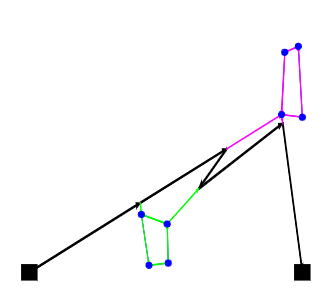
\includegraphics{asynchronous.png}
\caption{Feasible solution with partial overlapping that is not feasible for the complete overlapping model.}
\label{fig:proof2}
\end{figure}
% \begin{figure}[h!]
% \centering
% 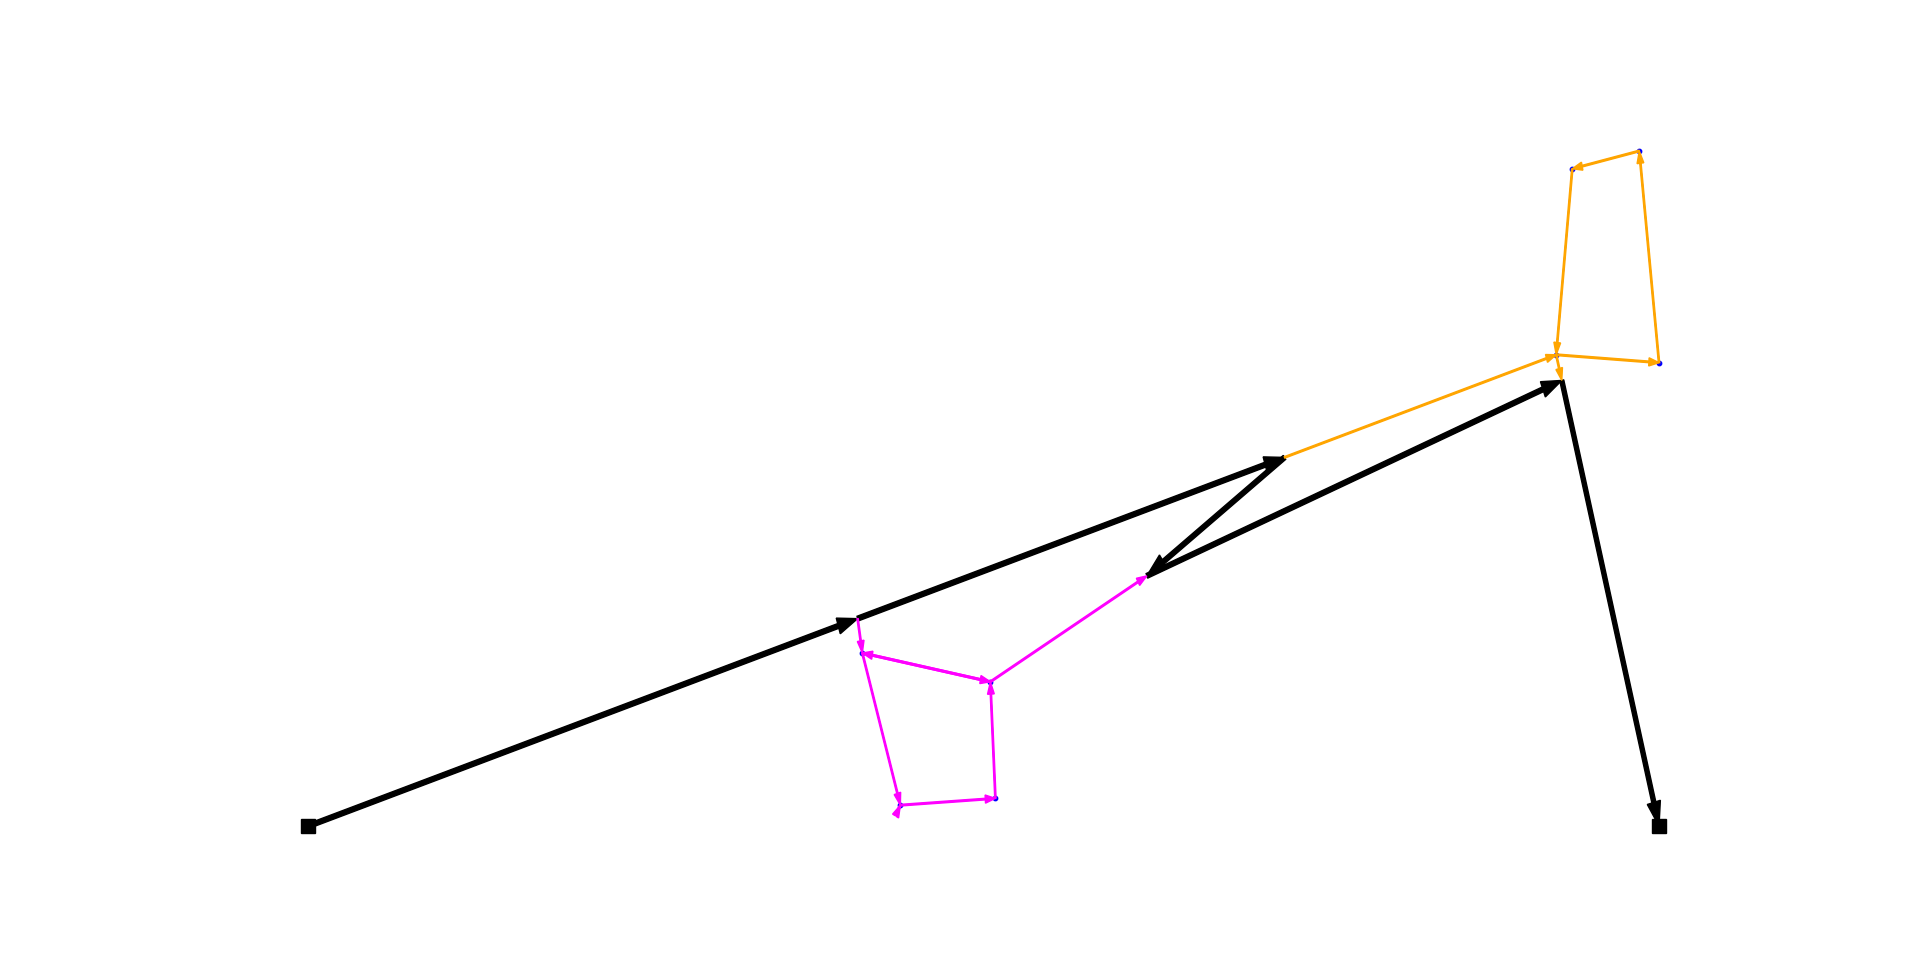
\includegraphics[width=0.6\linewidth]{figures/Asynchronous2-1-46-2.png}
% \end{figure}

\noindent
\RE{To} present our next result, wlog, we restrict ourselves to the degenerate case where graphs reduce to points. \RE{The reader may note that it is possible to reduce the visit of graphs to the visit of points by assuming that the drone is stopped in the point which is at same time that the one required to traverse the edges of the graph. We simplify the proof considering a generic solution between two consecutive target points.}


\begin{theorem}\label{thm:relationship}
Let $x_L^1$, $x_L^2$ (resp. $x_R^1$, $x_R^2$) be the launching (resp. rendezvous) points associated \RE{with} the visit of the target points $P_1$ and $P_2$. If there exist two points $x_L$ and $x_R$ verifying 
$$
 \left\{
 \begin{array}{ccl}
  \dfrac{\|x_L-x_R\|}{v_M} & \leq    & \dfrac{\|x_L - P_1\| + \|P_1 - x_R\|}{v_D}, \\
  \dfrac{\|x_L-x_R\|}{v_M} & \leq    & \dfrac{\|x_L - P_2\| + \|P_2 - x_R\|}{v_D}, \\
  \dfrac{\|x_L-x_R\|}{v_M} & \leq   & N_D, \\
  \|x_L-x_R\| & \leq & \|x_L^1 - x_L^2\| + \|x_L^2- x_R^1\| + \|x_R^1-x_R^2\|,
 \end{array}
 \right.
$$

\noindent then the contribution of this partial route to the optimal objective value will be the same in both models.
\end{theorem}
\begin{figure}[h!]
    \centering
    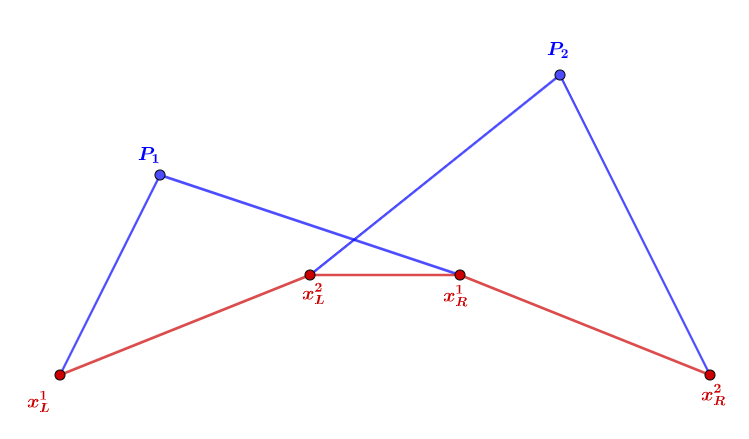
\includegraphics[width = 0.5\linewidth]{proof1.PNG}
    \caption{The mothership launches two drones sequentially}
    \label{fig:proof1}
\end{figure}

\begin{proof}
Note that in the considered configuration, the order of visit\RE{s} to the points $P_1$ and $P_2$ is fixed and then, the binary variables in the model are fixed in this case. Thus, the only difference\RE{s} that the two models can have are the location of the launching and rendezvous points. Hence, the only constraints that are involved are those related to these points. These are the conditions in the statement: The first two are the \eqref{DCW} inequalities. The third one is the \eqref{CAP} constraint and the last one ensures that the distance traveled by the mothership in the \RE{complete overlapping} model is smaller than or equal to the distance assumed in the \RE{partial overlapping} solution described in the statement. Therefore, the conclusion follows.
\end{proof}

\noindent
\RE{Note that this result states sufficient conditions to obtain the same solution for the two models.% \CV{DISCUSS: More implications and meanings?}
}

}
\color{black}
%(Meto restricción de capacidad? para hacer experimentos puede complicarse)

% $$
% e=(i, j) \ni x_R^t \rightarrow V_i \vee V_j \rightarrow \ldots \rightarrow V_k \rightarrow \ldots \rightarrow V_{i'} \rightarrow x_L^{t+1} \in (i',j')=e'
% $$

% The design of these paths obeys to define binary variables that decide which vertices are selected in each stage $t$: 
%
\section{Formulation draft}
In the following formulation we use the concept of \emph{stage} to refer the action of receiving or launching a drone from the mothership. Each graph must be visited by a drone so that \LA{each operation} gives rise to two stages: one when the drone is launched and another one once the same drone is retrieved by the mothership. We denote by $\matchal{T}$ the set of stages. It is clear that $|\mathcal{T}|=2|\mathcal{G}|$. Using the concept of stage we can \LA{substitute the set of operations with the set of stages to} model the coordination between drones and mothership in the asynchronous \LA{version of the problem. Indeed, in this case, differently from the synchronized version of the problem, the launch of a drone it is not necessarily followed by its retrieving but, for example, by the launch of a different drone to visit another target graph, like shown in figure \ref{fig:}. For this reason, we need to } 

\begin{comment}
\begin{table}[h!]
%\tiny
\scriptsize
\centering
%\color{blue}
\begin{tabular}{|l|}
\hline 
\textbf{Binary and Integer Decision Variables}\\
\hline
$\mu^{e_g} \in \{0,1\} \:\: \forall e_g \in E_g$ ($g \in \mathcal{G}$): equal to 1 if edge $e$ of graph $g$ (or a portion of it) is visited by the drone,\\ \hspace*{1cm} and  0 otherwise.\\
$\gamma^{go}\in \{0,1\}$ \\
$u^{go} \in \{0,1\} \:\: \forall g \in \mathcal{G} \: \forall o \in \Theta  \: \forall d \in \mathcal D$: equal to 1 if the visit of graph $g$ starts in operation $o$, 0 otherwise.\\
$z^{e_{g}e^{'}_{g}} \in \{0,1\} \:\: \forall e_g, e_g' \in E_g$ ($g \in \mathcal{G}$): equal to 1 if the drone goes from $e_g$ to $e^{'}_{g}$, 0 otherwise.\\
$v^{go} \in \{0,1\} \:\: \forall g \in \mathcal{G} \: \forall o \in \Theta$: equal to 1 if the the visit of graph $g$ ends in operation $o$, 0 otherwise.\\
$in^{e_g} \in \{0,1\} \:\: \forall e_g \in E_g$ ($g \in \mathcal{G}$): equal to 1 if the the visit of graph $g$ starts from edge $e_g$, 0 otherwise.\\
$out^{e_g} \in \{0,1\} \:\: \forall e_g \in E_g$ ($g \in \mathcal{G}$): equal to 1 if the the visit of graph $g$ ends in edge $e_g$, 0 otherwise.\\
$y_{LL}^o \:\: \forall o \in \Theta$, equal to 1 if the mothership moves from a launching point to a launching point between operation $o$\\ \hspace*{1cm} and operation $o+1$, 0 otherwise.\\
$y_{LR}^o \:\: \forall o \in \Theta$, equal to 1 if the mothership moves from a launching point to a retrieving point between operation $o$\\ \hspace*{1cm} and operation $o+1$, 0 otherwise.\\
$y_{RL}^o \:\: \forall o \in \Theta$ equal to 1 if the mothership moves from a retrieving point to a launching point between operation $o$\\ \hspace*{1cm} and operation $o+1$, 0 otherwise.\\
$y_{RR}^o \:\: \forall o \in \Theta$ equal to 1 if the mothership moves from a retrieving point to a retrieving point between operation $o$\\ \hspace*{1cm} and operation $o+1$, 0 otherwise.\\
$\mathcal{K}(o) \:\: \forall o \in \Theta$, integer non-negative variable representing the number of available drones at operation $o$.\\
\hline
\textbf{Continuous Decision Variables}\\
\hline
$x_L^o \:\: \forall o \in \Theta$: coordinates representing the launching point visited by the mothership at operation $o$.\\
$x_R^o \:\: \forall o \in \Theta$: coordinates representing the retrieving point visited by the mothership at operation $o$.\\
$R^{e_g} \:\: \forall e_g \in E_g$ ($g \in \mathcal{G}$): coordinates representing the entry point on edge $e_g$ of graph $g$.\\
$L^{e_g} \:\: \forall e_g \in E_g$ ($g \in \mathcal{G})$: coordinates representing the exit point on edge $e_g$ of graph $g$.\\
$d_L^{e_g o} \geq 0, \:\: \forall e_g \in E_g$ ($g \in \mathcal{G}$) $\forall o \in \Theta$: representing the distance travelled by the drone from the launching\\
\hspace*{1cm} point $x_L^o$ on the mothership at operation $o$ to the first visiting point $R^{e_g}$ on $e_g$.\\
$d^{e_ge^\prime_g} \geq 0, \:\: \forall e_g, e^\prime_g \in E_g $ ($g \in \mathcal{G}$): representing the distance travelled by the drone from the launching point $L^{e_g}$ on $e_g$ to\\
\hspace*{1cm}  the rendezvous point $R^{e^\prime_g}$ on $e^\prime_g$.\\
$d^{e_g} \geq 0, \:\: \forall e_g \in E_g$ ($g \in \mathcal{G}$): representing the distance travelled by the drone from the rendezvous point $R^{e_g}$ to the \\
\hspace*{1cm} launching point $L^{e_g}$ on $e_g$. \\
$d_R^{e_g o} \geq 0 \:\: \forall e_g \in E_g$ ($g \in \mathcal{G}$) $\forall o \in \Theta$: representing the distance travelled by the drone from the last visiting point\\
\hspace*{1cm} $L^{e_g}$ on $e_g$ to the rendezvous point $x_R^o$ on the mothership at operation $o$.\\
$d_{LR}^g \geq 0 \:\: \forall g \in\mathcal G$: representing the distance travelled by the mothership from the launching point $x_L^o$ to the rendezvous\\
\hspace*{1cm} point $x_R^o$ associated with graph $g$ for some $o \in \Theta$.\\
\hline
\end{tabular}
\caption{Decision Variables for AMMDRPG}
\label{table:t2}
\end{table}


\textbf{Drone Constraints}

\begin{equation}
    \sum_{o \in \Theta} u^{go} = 1 \:\: \forall g \in \mathcal{G}
\end{equation}

\begin{equation}
    \sum_{o \in \Theta} v^{go} = 1 \:\: \forall g \in \mathcal{G}
\end{equation}

\begin{equation}
    \sum_{e_g \in E_g} in^{e_g} \geq u^{go} \:\: \forall g \in \mathcal{G} \:\: \forall o \in \Theta
\end{equation}

\begin{equation}
    \sum_{e_g \in E_g} out^{e_g} \geq v^{go} \:\: \forall g \in \mathcal{G} \:\: \forall o \in \Theta
\end{equation}

\begin{equation}
    \sum_{e_g \in E_g} in^{e_g} = 1\:\: \forall g \in \mathcal{G}
\end{equation}

\begin{equation}
    \sum_{e_g \in E_g} out^{e_g} = 1\:\: \forall g \in \mathcal{G}
\end{equation}

\begin{equation}
    \sum_{g \in \mathcal{G}} (u^{go} + v^{go}) \leq \mathcal{K}(o) \:\: \forall o \in \Theta
\end{equation}
\begin{equation}
    \sum_{g \in \mathcal{G}} (u^{go} + v^{go}) \leq 1 \:\: \forall o \in \Theta
\end{equation}
\begin{equation}
    u^{go} \leq \gamma^{go} \:\:\ \forall g \in \mathcal{G} \:\: \forall o \in \Theta
\end{equation}

\begin{equation}
    in^{e_go} + \sum_{e_g' \in E_g} z^{e_g' e_g} \leq \mu^{e_g} \:\:\ \forall e_g \in E_g: \:\: g \in \mathcal G
\end{equation}

\begin{equation}
   out^{e_go} + \sum_{e_g' \in E_g} z^{e_g e_g'} \leq \mu^{e_g} \:\:\ \forall e_g \in E_g: \:\:  g \in \mathcal G
\end{equation}

\begin{equation}
   \gamma^{g(o+1)} \geq \gamma^{go} - v^{go} \:\:\ \forall g \in \mathcal{G} \:\: \forall o \in \Theta: o < |\Theta|
\end{equation}
\begin{equation}
   \mathcal{K}(1) = |\mathcal{D}|
\end{equation}
\begin{equation}
   \mathcal{K}(o) = \mathcal{K}(o-1) + \sum_{g\in\mathcal G}v^{g(o-1)} - \sum_{g\in\mathcal G}u^{g(o-1)} \:\:\ \forall o \in \Theta: o>1
\end{equation}

\textbf{Mothership Constraints}

\begin{equation}
   y_{LL}^1 + y_{LR}^1 = 1
\end{equation}
\begin{equation}
   y_{LL}^o + y_{LR}^o \geq y_{RL}^{o-1} + y_{LL}^{o-1} \:\: \forall o \in \Theta: o>1
\end{equation}
\begin{equation}
   y_{RR}^o + y_{RL}^o \geq  y_{LR}^{o-1} + y_{RR}^{o-1} \:\: \forall o \in \Theta: o>1
\end{equation}
\begin{equation}
   y_{LR}^{|\Theta|} + y_{RR}^{|\Theta|} = 1 
\end{equation}

\textbf{Mothership Distance}

\begin{equation}
   d_M = \sum_{o \in \Theta: o < |\Theta|} (\|x_L^o - x_L^{o+1}\|y_{LL}^o + \|x_L^o - x_R^{o+1}\|y_{LR}^o + \|x_R^o - x_L^{o+1}\|y_{RL}^o + \| x_R^o - x_R^{o+1}\|y_{RR}^o )
\end{equation}

\textbf{Distance associated to graph g}

\begin{equation}
   d_{LR}^g = \sum_{o \in \Theta: o < |\Theta|} (\|x_L^o - x_L^{o+1}\|y_{LL}^o + \|x_L^o - x_R^{o+1}\|y_{LR}^o + \|x_R^o - x_L^{o+1}\|y_{RL}^o + \| x_R^o - x_R^{o+1}\|y_{RR}^o )\gamma^{go} \:\:\ \forall g \in \mathcal{G}
\end{equation}

\textbf{Coordination Constraint}
\begin{equation}
\frac{1}{v_D}\left(\sum_{o \in \Theta} \sum_{e_g \in E_g} in^{e_g}d_L^{e_g o} + \sum_{e_g, e^\prime_g\in E_g}z^{e_ge^\prime_g}d^{e_ge^\prime_g} + \sum_{e_g\in E_g} \mu^{e_g}d^{e_g} + \sum_{o \in \Theta} \sum_{e_g \in E_g}out^{e_g}d_R^{e_g o}\right) \leq \frac{d_{LR}^g}{v_M} \:\: \forall g \in \mathcal{G}
\end{equation}

\textbf{Linearization Constraints}

\begin{equation}
   y_{LR}^o \leq \sum_{g \in \mathcal{G}} u^{go} \:\: \forall o \in \Theta
\end{equation}
\begin{equation}
   y_{LR}^o \leq \sum_{g \in \mathcal{G}} v^{g(o+1)} \:\: \forall o \in \Theta: o < |\Theta|
\end{equation}
\begin{equation}
   y_{LR}^o \geq \sum_{g \in \mathcal{G}} u^{go} + \sum_{g \in \mathcal{G}} v^{g(o+1)} -1 \:\: \forall o \in \Theta: o < |\Theta|
\end{equation}

\begin{equation}
   y_{LL}^o \leq \sum_{g \in \mathcal{G}} u^{go} \:\: \forall o \in \Theta
\end{equation}
\begin{equation}
   y_{LL}^o \leq \sum_{g \in \mathcal{G}} u^{g(o+1)} \:\: \forall i \in \Theta: o < |\Theta|
\end{equation}
\begin{equation}
   y_{LL}^o \geq \sum_{g \in \mathcal{G}} u^{go} + \sum_{g \in \mathcal{G}} u^{g(o+1)} -1 \:\: \forall o \in \Theta: o < |\Theta|
\end{equation}

\begin{equation}
   y_{RR}^o \leq \sum_{g \in \mathcal{G}} v^{go} \:\: \forall o \in \Theta
\end{equation}
\begin{equation}
   y_{RR}^o \leq \sum_{g \in \mathcal{G}} v^{g(o+1)} \:\: \forall o \in \Theta: o < |\Theta|
\end{equation}
\begin{equation}
   y_{RR}^o \geq \sum_{g \in \mathcal{G}} v^{go} + \sum_{g \in \mathcal{G}} v^{g(o+1)} -1 \:\: \forall o \in \Theta: o < |\Theta|
\end{equation}

\begin{equation}
   y_{RL}^o \leq \sum_{g \in \mathcal{G}} v^{go} \:\: \forall o \in \Theta
\end{equation}
\begin{equation}
   y_{RL}^o \leq \sum_{g \in \mathcal{G}} u^{g(o+1)} \:\: \forall o \in \Theta: o < |\Theta|
\end{equation}
\begin{equation}
   y_{RL}^o \geq \sum_{g \in \mathcal{G}} v^{go} + \sum_{g \in \mathcal{G}} u^{g(o+1)} -1 \:\: \forall o \in \Theta: o < |\Theta|
\end{equation}
\end{comment}



\begin{table}[h]
%\tiny
\scriptsize
\centering
%\color{blue}
\begin{tabular}{|l|}
\hline 
\textbf{Binary and Integer Decision Variables}\\
\hline
$\mu^{e_g} \in \{0,1\} \:\: \forall e_g \in E_g$ ($g \in \mathcal{G}$): equal to 1 if edge $e$ of graph $g$ (or a portion of it) is visited by the drone,\\ \hspace*{1cm} and  0 otherwise.\\
$\text{entry}^{e_g} \in \{0,1\} \:\: \forall e_g \in E_g$ ($g \in \mathcal{G}$): auxiliary binary variable used for linearizing expressions.\\
$u^{e_g o} \in \{0,1\} \:\: \forall e_g \in E_g \:\: (g \in \mathcal{G}) \:\: \forall o \in \Theta$: equal to 1 if the visit of graph $g$ starts in event $o$ from edge $e_g$, 0 otherwise.\\
$z^{e_{g}e^{'}_{g}} \in \{0,1\} \:\: \forall e_g, e_g' \in E_g$ ($g \in \mathcal{G}$): equal to 1 if the drone goes from $e_g$ to $e^{'}_{g}$, 0 otherwise.\\
\LA{$\gamma^{go}\in \{0,1\}$: equal to 1 if the operation of visiting graph $g$ continues when event $o$ occurs, 0 otherwise.}\\
$v^{e_g o} \in \{0,1\} \:\: \forall g \in E_g \:\: (g \in \mathcal{G}) \: \forall o \in \Theta$: equal to 1 if the the visit of graph $g$ ends in event $o$ on edge $e_g$, 0 otherwise.\\
%$in^{e_g} \in \{0,1\} \:\: \forall e_g \in E_g$ ($g \in \mathcal{G}$): equal to 1 if the the visit of graph $g$ starts from edge $e_g$, 0 otherwise.\\
%$out^{e_g} \in \{0,1\} \:\: \forall e_g \in E_g$ ($g \in \mathcal{G}$): equal to 1 if the the visit of graph $g$ ends in edge $e_g$, 0 otherwise.\\
$y_{LL}^o \in \{0,1\}  \:\: \forall o \in \Theta:o<|\Theta|$: equal to 1 if the mothership moves from a launching point to a launching point between event $o$\\ \hspace*{1cm} and event $o+1$, 0 otherwise.\\
$y_{LR}^o \in \{0,1\}  \:\: \forall o \in \Theta:o<|\Theta|$: equal to 1 if the mothership moves from a launching point to a retrieving point between event $o$\\ \hspace*{1cm} and event $o+1$, 0 otherwise.\\
$y_{RL}^o \in \{0,1\}  \:\: \forall o \in \Theta:o<|\Theta|$: equal to 1 if the mothership moves from a retrieving point to a launching point between event $o$\\ \hspace*{1cm} and event $o+1$, 0 otherwise.\\
$y_{RR}^o \in \{0,1\}  \:\: \forall o \in \Theta:o<|\Theta|$: equal to 1 if the mothership moves from a retrieving point to a retrieving point between event $o$\\ \hspace*{1cm} and event $o+1$, 0 otherwise.\\
$\mathcal{K}(o) \in \{0, 1, 2, \ldots, |\mathcal D|\}  \:\: \forall o \in \Theta$: integer non-negative variable representing the number of available drones at event $o$.\\
\hline
\textbf{Continuous Decision Variables}\\
\hline
$s^{e_g} \:\: \forall e_g \in E_g$ ($g \in \mathcal{G}$): continuous non negative variable representing the order of visit of the edge $e$ of graph $g$.\\
$x_L^o \:\: \forall o \in \Theta$: coordinates representing the launching point visited by the mothership at event $o$.\\
$x_R^o \:\: \forall o \in \Theta$: coordinates representing the retrieving point visited by the mothership at event $o$.\\
$R^{e_g} \:\: \forall e_g \in E_g$ ($g \in \mathcal{G}$): coordinates representing the entry point on edge $e_g$ of graph $g$.\\
$L^{e_g} \:\: \forall e_g \in E_g$ ($g \in \mathcal{G})$: coordinates representing the exit point on edge $e_g$ of graph $g$.\\
$d_L^{e_g o} \geq 0, \:\: \forall e_g \in E_g$ ($g \in \mathcal{G}$) $\forall o \in \Theta$: representing the distance travelled by the drone from the launching\\
\hspace*{1cm} point $x_L^o$ on the mothership at event $o$ to the first visiting point $R^{e_g}$ on $e_g$.\\
$d^{e_g} \geq 0, \:\: \forall e_g \in E_g$ ($g \in \mathcal{G}$): representing the distance travelled by the drone from the rendezvous point $R^{e_g}$ to the \\
\hspace*{1cm} launching point $L^{e_g}$ on $e_g$. \\
$d^{e_ge^\prime_g} \geq 0, \:\: \forall e_g, e^\prime_g \in E_g $ ($g \in \mathcal{G}$): representing the distance travelled by the drone from the launching point $L^{e_g}$ on $e_g$ to\\
\hspace*{1cm}  the rendezvous point $R^{e^\prime_g}$ on $e^\prime_g$.\\
$d_R^{e_g o} \geq 0 \:\: \forall e_g \in E_g$ ($g \in \mathcal{G}$) $\forall o \in \Theta$: representing the distance travelled by the drone from the last visiting point\\
\hspace*{1cm} $L^{e_g}$ on $e_g$ to the rendezvous point $x_R^o$ on the mothership at event $o$.\\
$d_{origin}\geq 0$: distance from the origin $origin$ to the first launching point $x_L^1$.\\
$d_{LL}^o\geq 0 \:\: \forall o \in \Theta:o<|\Theta|$: distance from the launching point $x_L^o$ to the launching point $x_L^{o+1}$.\\
$d_{LR}^o\geq 0 \:\: \forall o \in \Theta:o<|\Theta|$: distance from the launching point $x_L^o$ to the retrieving point $x_R^{o+1}$.\\
$d_{RL}^o\geq 0 \:\: \forall o \in \Theta:o<|\Theta|$: distance from the retrieving point $x_R^o$ to the launching point $x_L^{o+1}$.\\
$d_{RR}^o\geq 0 \:\: \forall o \in \Theta:o<|\Theta|$: distance from the retrieving point $x_R^o$ to the retrieving point $x_R^{o+1}$.\\
$d_{dest}\geq 0$: distance from the last retrieving point $x_R^{|\Theta|}$ to the destination $dest$.\\
$d_{LR}^g\geq 0 \:\: \forall g \in\mathcal G$: representing the distance travelled by the mothership from the launching point $x_L^o$ to the rendezvous\\
\hspace*{1cm} point $x_R^{o'}$ associated with graph $g$ for some $o, o' \in \Theta$.
\hline
\end{tabular}
\caption{Decision Variables for AMMDRPG - asynchronous version }
\label{table:t3}
\end{table}

\clearpage

%\textbf{Alternative formulation with less constraints}


\CV{
In the following, we arrange the constraints that model the coordination system in the following subsections: drone constraints, mothership constraints, distance constraints, coordination and endurance constraints and linearization constraints.

\subsection*{Drone Constraints}
\noindent
\LA{Similarly to the synchronous version of the problem, we model the route followed by the drone by using the binary variables $u^{e_g o}$, $v^{e_g o}$ and $z^{e_g e_g'}$. However, in this case, the variables $u^{e_g o}$ and $v^{e_g o}$ are associated  with the event $o$ and because of the problem assumptions, we need to introduce the additional binary variables $\gamma^{go}$ .} 
\LA{Thus,} the following constraints model the route followed by the drone while it is operating in a graph $g\in \mathcal G$:
}
\begin{footnotesize}
\begin{align}
\sum_{o \in \Theta} \sum_{e_g\in E_g} u^{e_g o} &= 1, &\forall g \in \mathcal{G}, \label{eq:drone1}\\ 
\sum_{o \in \Theta} \sum_{e_g\in E_g} v^{e_g o} &= 1, &\forall g \in \mathcal{G}, \label{eq:drone2}\\
\sum_{g\in\mathcal {G}} \sum_{e_g \in E_g} u^{e_g o} &\leq \mathcal{K}(o), &\forall o \in \Theta, \label{eq:drone3}\\
\sum_{g\in\mathcal {G}} \sum_{e_g \in E_g} (u^{e_g o} + v^{e_g o}) &\leq 1, &\forall o \in \Theta, \label{eq:drone4}\\
\sum_{e_g \in E_g} u^{e_g o} &\leq \sum_{e_g \in E_g} \sum_{o' \in \Theta: o'>o} v^{e_g o'}, &\forall g\in\mathcal G, \:\: \forall o \in \Theta, \label{eq:drone5}\\
\sum_{o \in \Theta} u^{e_g o} + \sum_{e_g' \in E_g}z^{e_g'e_g} &= \mu^{e_g}, &\forall e_g \in E_g: \:\:  g \in \mathcal{G}, \label{eq:drone6}\\
\sum_{o \in \Theta} v^{e_g o} + \sum_{e_g' \in E_g}z^{e_g e_g'} &= \mu^{e_g}, &\forall e_g \in E_g: \:\: g \in \mathcal{G}, \label{eq:drone7}\\
\gamma^{go} &\geq \sum_{e_g \in E_g} u^{e_g o}, &\forall g \in \mathcal{G}, \:\: \forall o \in \Theta, \label{eq:drone8}\\
\gamma^{g(o+1)} &\geq \gamma^{go} - \sum_{e_g \in E_g} v^{e_g (o+1)},  &\forall g \in \mathcal{G}, \:\: \forall o \in \Theta: o < |\Theta|, \label{eq:drone9}\\
\sum_{o'\in\Theta : o' < o} \gamma^{go'} &\leq (o-1)(1- \sum_{e_g\in E_g} u^{e_g o}), &\forall g\in\mathcal G, \:\: \forall o \in \Theta, \label{eq:drone10}\\
\sum_{o' \in \Theta: o' \geq o} \gamma^{go'} &\leq \left(|\Theta| - o + 1\right) (1- \sum_{e_g\in E_g}v^{e_g o}), &\forall g\in\mathcal G, \:\: \forall o \in \Theta, \label{eq:drone11}\\
\mathcal{K}(1) &= |\mathcal{D}|, \label{eq:drone12}\\
\mathcal{K}(o+1) &= \mathcal{K}(o) + \sum_{g\in\mathcal {G}} \sum_{e_g \in E_g} v^{e_g o} - \sum_{g\in\mathcal G}\sum_{e_g \in E_g} u^{e_g o}, &\forall o \in \Theta: o<|\Theta|. \label{eq:drone13}
\end{align}
\end{footnotesize}

\CV{Constraints \eqref{eq:drone1} and \eqref{eq:drone2} ensure that a launching and a retrieving points are associated to each graph $g$. Constraints \eqref{eq:drone3} allow the mothership to launch a drone in the event $o$ if only a drone is available when the event $o$ occurs. Constraints \eqref{eq:drone4} guarantee that a launching or a retrieving occurs in each event $o\in\Theta$. Constraints \eqref{eq:drone5} indicate that the retrieving event associated to the graph $g$ happens after the launching event associated to the same graph $g$. Equations \eqref{eq:drone6} (resp. \eqref{eq:drone7}) state that the number of exterior edges plus the number of interior edges that enter (resp. exit) to the edge $e_g$ is given by $\mu^{e_g}$.
Constraints \eqref{eq:drone8} ensure that the operation associated with graph $g$ starts when the drone is launched during the event $o$. Inequalities \eqref{eq:drone9} state that the drone is still operating in graph $g$ for successive events until it is retrieved in the event $o$. Constraints \eqref{eq:drone10} ensure that the drone is not operating in $g$ until the event of launching occurs. Constraints \eqref{eq:drone11} guarantee that the drone finishes operating in the graph $g$ when the event of retrieving happens. Finally, constraints \eqref{eq:drone12} and \eqref{eq:drone13} model the number of available drones at the event $o$.

}

\CV{
\subsection*{Mothership Constraints}
In this subsection, we model all the configurations that the mothership can follow in the succession of events in terms of launching and retrieving:
}
\begin{align}
   y_{LL}^1 + y_{LR}^1 & = 1, \label{eq:mother1}\\
   y_{LL}^{o+1} + y_{LR}^{o+1} & \geq y_{RL}^{o} + y_{LL}^{o}, &\forall o \in \Theta: o<|\Theta|,\label{eq:mother2}\\
   y_{RR}^{o+1} + y_{RL}^{o+1} & \geq  y_{LR}^{o} + y_{RR}^{o}, &\forall o \in \Theta: o<|\Theta|,\label{eq:mother3}\\
   y_{LR}^{|\Theta|-1} + y_{RR}^{|\Theta|-1} & = 1. \label{eq:mother4}
\end{align}

\CV{Constraints \eqref{eq:mother1} state that in event 1 the mothership must depart from the launching point $x_L^1$. Constraints \eqref{eq:mother2} (resp. \eqref{eq:mother3}) ensure that if the mothership go to the launching (resp. retrieving) point $x_L^{o+1}$ (resp. $x_R^{o+1}$) then in the next event it must depart from $x_L^{o+1}$ (resp. $x_R^{o+1}$). Constraint \eqref{eq:mother4} guarantee that the path followed by the mothership finishes in the retrieving point $x_R^{|\Theta|}$.}

\CV{
\subsection*{Distance Constraints}
This subsection considers the second-order cone constraints that model the distances covered either by the drone and mothership:
}
\begin{align*}
\|x_L^o- R^{e_g}\| & \leq  d_L^{e_go},  &\forall e_g:g\in \mathcal{G}, \:\:\forall o\in \Theta, \tag{Drone DIST$_{1}$} \label{eq:drone-d1-async}\\
\|R^{e_g}- L^{e_g}\| & \leq  d^{e_g},  &\forall e_g:g\in \mathcal{G}, \tag{Drone DIST$_{2}$} \label{eq:drone-d2-async}\\
\|R^{e_g}- L^{e'_g}\| & \leq  d^{e_ge'_g}, &\forall e_g\neq e_g'\in E_g:g\in \mathcal{G}, \tag{Drone DIST$_{3}$} \label{eq:drone-d3-async}\\
\|L^{e_g}- x_R^o\| & \leq  d_R^{e_go}, &\forall e_g:g\in \mathcal{G},\:\:\forall o\in \Theta. \tag{Drone DIST$_{4}$} \label{eq:drone-d4-async}\\\\
\|origin - x_L^1\| & \leq d_{origin}, \tag{Mothership DIST$_1$}\label{eq:mothership-d1-async}\\
\|x_L^o - x_L^{o+1}\| & \leq d_{LL}^{o}, &\forall o\in\Theta:o<|\Theta|, \tag{Mothership DIST$_{2}$}\label{eq:mothership-d2-async}\\
\|x_L^o - x_R^{o+1}\| & \leq d_{LR}^{o}, &\forall o\in\Theta:o<|\Theta|, \tag{Mothership DIST$_{3}$}\label{eq:mothership-d3-async}\\
\|x_R^o - x_L^{o+1}\| & \leq d_{RL}^{o}, &\forall o\in\Theta:o<|\Theta|, \tag{Mothership DIST$_{4}$}\label{eq:mothership-d4-async}\\
\|x_R^o - x_R^{o+1}\| & \leq d_{RR}^{o}, &\forall o\in\Theta:o<|\Theta|, \tag{Mothership DIST$_{5}$}\label{eq:mothership-d5-async}\\
\|x_R^{|\Theta|} - dest\| & \leq d_{dest}. \tag{Mothership DIST$_6$}\label{eq:mothership-d6-async}
\end{align*}

\CV{
Drone distance variables $d_L^{e_go}$, $d^{e_g}$, $d^{e_g'e_g}$ and $d_R^{e_go}$ as well as mothership distance variables $d_{origin}$, $d_{LL}^o$, $d_{LR}^o$, $d_{RL}^o$, $d_{RR}^o$ and $d_{dest}$ are all defined in Table \ref{table:t3}. 

The time spent by the drone to make the operation of visiting graph $g$ is given by:
}

\begin{footnotesize}
\begin{equation}\tag{Time$^g_D$}\label{eq:time-g-d}
time_D^g = \frac{1}{v_D}\left(\sum_{o \in \Theta}\sum_{e_g \in E_g} u^{e_g o}d_L^{e_g o} + \sum_{e_g, e^\prime_g\in E_g}z^{e_ge^\prime_g}d^{e_ge^\prime_g} + \sum_{e_g\in E_g} \mu^{e_g}d^{e_g} + \sum_{o \in \Theta}\sum_{e_g \in E_g} v^{e_g o}d_R^{e_g o}\right).
\end{equation}
\end{footnotesize}

\CV{
The time spent by the mothership while the drone is operating in the graph $g$ is given by:
}

\begin{footnotesize}
\begin{equation}\tag{Time$^g_M$}\label{eq:time-g-m}
   time_M^g = \frac{1}{v_M} d_{LR}^g = \frac{1}{v_M}\sum_{o \in \Theta: o < |\Theta|} (\|x_L^o - x_L^{o+1}\|y_{LL}^o + \|x_L^o - x_R^{o+1}\|y_{LR}^o + \|x_R^o - x_L^{o+1}\|y_{RL}^o + \| x_R^o - x_R^{o+1}\|y_{RR}^o )\gamma^{go}, \:\:\ \forall g \in \mathcal{G}.
\end{equation}
\end{footnotesize}

\CV{
Finally, the overall time spent by the mothership can be described as follows:
}
\begin{footnotesize}
\begin{equation}\tag{Time$_M$}\label{eq:time-m}
time_M = \frac{1}{v_M}\left(d_{origin} + \sum_{o \in \Theta: o < |\Theta|} \left(\|x_L^o - x_L^{o+1}\|y_{LL}^o + \|x_L^o - x_R^{o+1}\|y_{LR}^o + \|x_R^o - x_L^{o+1}\|y_{RL}^o + \| x_R^o - x_R^{o+1}\|y_{RR}^o\right) + d_{dest} \right).
\end{equation}
\end{footnotesize}

\CV{
\subsection*{Coordination and endurance constraints}
Once defined the time spent by the drone to visit the graph $g$ and the time spent by the mothership while the drone is visiting this graph $g$, we can model the coordination constraint simply as:
}
\begin{equation}\label{eq:DCW-Overlapping}\tag{DCW-Overlapping}
    time_D^g \leq time_M^g,\quad\forall g\in\mathcal G.
\end{equation}

In addition, the time spent by the drone to operate in the graph $g$ must not exceed its endurance:

\begin{equation}\label{eq:Endurance-Overlapping}\tag{Endurance-Overlapping}
    time_D^g \leq N_D
\end{equation}


\CV{
\subsection*{Linearization Constraints}
This subsection is devoted to linearize the relationship between the decision variables that model the route of the mothership and the drones. For each $o\in\Theta\setminus \{|\Theta|\}$, the relationship of these variables is given by the products
}
\begin{align*}
    y_{LL}^o & = \sum_{g\in\mathcal G}\sum_{e_g\in E_g} u^{e_go} \sum_{g\in\mathcal G}\sum_{e_g\in E_g} u^{e_g(o+1)},\\
    y_{LR}^o & = \sum_{g\in\mathcal G}\sum_{e_g\in E_g} u^{e_go} \sum_{g\in\mathcal G}\sum_{e_g\in E_g} v^{e_g(o+1)},\\
    y_{RL}^o & = \sum_{g\in\mathcal G}\sum_{e_g\in E_g} v^{e_go} \sum_{g\in\mathcal G}\sum_{e_g\in E_g} u^{e_g(o+1)},\\
    y_{RR}^o & = \sum_{g\in\mathcal G}\sum_{e_g\in E_g} v^{e_go} \sum_{g\in\mathcal G}\sum_{e_g\in E_g} v^{e_g(o+1)}.\\
\end{align*}

\CV{
These products can be linearized, respectively, by means of these constraints:
}

\begin{align}
   y_{LL}^o &\leq \sum_{g\in\mathcal {G}} \sum_{e_g \in E_g} u^{e_g o},\label{eq:yLL-1}\\%{$y_{LL}$-1}\\
   y_{LL}^o &\leq \sum_{g\in\mathcal {G}} \sum_{e_g \in E_g} u^{e_g (o+1)},\\%{$y_{LL}$-2}\\
   y_{LL}^o &\geq \sum_{g\in\mathcal {G}} \sum_{e_g \in E_g} u^{e_g o} + \sum_{g\in\mathcal {G}} \sum_{e_g \in E_g} u^{e_g (o+1)} -1,\\%{$y_{LL}$-3}\\\\
   y_{LR}^o &\leq \sum_{g\in\mathcal {G}} \sum_{e_g \in E_g} u^{e_g o},\\%{$y_{LR}$-1}\\
   y_{LR}^o &\leq \sum_{g\in\mathcal {G}} \sum_{e_g \in E_g} v^{e_g (o+1)},\\%{$y_{LR}$-2}\\
   y_{LR}^o &\geq \sum_{g\in\mathcal {G}} \sum_{e_g \in E_g} u^{e_g o} + \sum_{g\in\mathcal {G}} \sum_{e_g \in E_g} v^{e_g (o+1)} -1,\\%{$y_{LR}$-3}\\\\
   y_{RL}^o &\leq \sum_{g\in\mathcal {G}} \sum_{e_g \in E_g} v^{e_g o},\\%{$y_{RL}$-1}\\
   y_{RL}^o &\leq \sum_{g\in\mathcal {G}} \sum_{e_g \in E_g} u^{e_g (o+1)},\\%{$y_{RL}$-2}\\
   y_{RL}^o &\geq \sum_{g\in\mathcal {G}} \sum_{e_g \in E_g} v^{e_g o} +\sum_{g\in\mathcal {G}} \sum_{e_g \in E_g} u^{e_g (o+1)} -1,\\%{$y_{RL}$-3}\\\\
   y_{RR}^o &\leq \sum_{g\in\mathcal {G}} \sum_{e_g \in E_g} v^{e_g o},\\%{$y_{RR}$-1}\\
   y_{RR}^o &\leq \sum_{g\in\mathcal {G}} \sum_{e_g \in E_g} v^{e_g (o+1)},\\%{$y_{RR}$-2}\\
   y_{RR}^o &\geq \sum_{g\in\mathcal {G}} \sum_{e_g \in E_g}v^{e_g o} +\sum_{g\in\mathcal {G}} \sum_{e_g \in E_g} v^{e_g (o+1)} -1.\label{eq:yRR-3}%{$y_{RR}$-3}
\end{align}

\CV{Hence, the formulation of the \AMD\xspace with overlapping operations is:}
\begin{mini*}|s|
 {}{time_M}{}{} \label{AMMDRPG-Overlapping} \tag{AMMDRPG-Partial Overlapping}
 \addConstraint{\eqref{eq:drone1}-\eqref{eq:drone13}}{}{}
 \addConstraint{\eqref{eq:mother1}-\eqref{eq:mother4}}{}{}
 \addConstraint{\eqref{eq:yLL-1}-\eqref{eq:yRR-3}}{}{}
 \addConstraint{\eqref{MTZ1}-\eqref{MTZ2}} \text{ or }  \eqref{SEC}
 \addConstraint{\eqref{eq:alpha-E} \text{ or } \eqref{eq:alpha-G}}{}{}
 \addConstraint{\eqref{eq:drone-d1-async}-\eqref{eq:drone-d1-async}}{}{} \addConstraint{\eqref{eq:mothership-d1-async}-\eqref{eq:mothership-d6-async}}{}{}
 \addConstraint{\eqref{eq:time-g-d}, \eqref{eq:time-g-m}, \eqref{eq:time-m}}{}{}
 \addConstraint{\eqref{eq:DCW-Overlapping}, \eqref{eq:Endurance-Overlapping}}{}{}
\end{mini*}

% The variables associated with each of the considered distances are described in Table \ref{table:t3}:


% \textbf{Mothership Distance}

% \begin{equation}
%   d_M = \sum_{o \in \Theta: o < |\Theta|} (\|x_L^o - x_L^{o+1}\|y_{LL}^o + \|x_L^o - x_R^{o+1}\|y_{LR}^o + \|x_R^o - x_L^{o+1}\|y_{RL}^o + \| x_R^o - x_R^{o+1}\|y_{RR}^o )
% 



% \textbf{Distance associated to graph g}

% \begin{equation}
%   d_{LR}^g = \sum_{o \in \Theta: o < |\Theta|} (\|x_L^o - x_L^{o+1}\|y_{LL}^o + \|x_L^o - x_R^{o+1}\|y_{LR}^o + \|x_R^o - x_L^{o+1}\|y_{RL}^o + \| x_R^o - x_R^{o+1}\|y_{RR}^o )\gamma^{go} \:\:\ \forall g \in \mathcal{G}
% 

% \textbf{Coordination Constraint}
% \begin{equation}
% \frac{1}{v_D}\left(\sum_{o \in \Theta}\sum_{e_g \in E_g} u^{e_g o}d_L^{e_g o} + \sum_{e_g, e^\prime_g\in E_g}z^{e_ge^\prime_g}d^{e_ge^\prime_g} + \sum_{e_g\in E_g} \mu^{e_g}d^{e_g} + \sum_{o \in \Theta}\sum_{e_g \in E_g} v^{e_g o}d_R^{e_g o}\right) \leq \frac{d_{LR}^g}{v_M} \:\: \forall g \in \mathcal{G}
% \end{equation}




% \section{Strengthening the formulations}\label{bounds} % of \ref{AMMDRPG}}\label{bounds}
\noindent
In this section\CV{,} we present some valid inequalities for \CV{\eqref{AMMDRPG}} that reinforce the formulation given in Subsection \ref{subsec:CO}. Moreover, the \eqref{DCW} and \eqref{eq:DCW-Overlapping} constraints have products of binary and continuous variables that, when they are linearized, produce \CV{bigM} constants that have to be tightened. This section also provides some bounds for these constants whenever it is possible. 

%\CV{*** This last sentence is not done yet -JUSTO dixit- ***}

%Notation here is not very good: we use C for clusters, centroids and the drone endurance. This must be improved.

\subsection{Valid inequalities for the \ref{AMMDRPG}}
\noindent
In this problem, we assume that the fleet has more than one drone since otherwise the problem reduces to \RE{the \textit{All Terrain Mothership and Drone routing problem with graphs}} that was already studied in \cite{art:Amorosi2021}. Therefore, if there exists \JP{an operation} in which more than one drone is launched, the mothership does not need to perform $|\mathcal G|$ different operations. Hence, most likely the model does not need to deal with those operations that are numbered at the end. By exploiting this idea, it is possible to concentrate all \RE{drone activities on the first operations, avoiding empty operations in $\mathcal{O}$.}
\noindent
Let $\beta^o$ be a binary variable that assumes the value one if all the target graphs are visited when the operation $o$ begins, and zero, otherwise. Note that, if all the graphs are already visited before the operation $o$ then they are also completed before the operation $o+1$. Hence, $\beta$ variables must satisfy the following constraints:

\begin{equation}\tag{Monotonicity}\label{eq:Monotonicity}
\beta^o \leq \beta^{o+1}, \mbox{ for all } o=1,\ldots, |\mathcal{G}|-1.
\end{equation}

\noindent
Let $k^o$ denote the number of graphs that are visited in the operation $o$. This number can be computed using the $u$ variables since $u^{e_go}$ takes the value 1 if the graph $g$ is visited in operation $o$. Thus:

$$k^o=\sum_{g\in\mathcal G}\sum_{e_g\in E_g} u^{e_go}.$$

\noindent
Hence, if $\beta^o$ equals one, the entire set of graphs in $\mathcal G$ must have been visited before the operation $o$:

\begin{equation}\tag{VI-1}\label{eq:VI-1}
\sum_{o'=1}^{o-1} k^{o'} \geq |\mathcal G|\beta^o, \quad\forall \RE{o\in\mathcal{O}},
\end{equation}
where $|\mathcal G|$ denotes the number of graphs of $\mathcal G$.

\noindent
To reduce the space of feasible solutions, we can assume without loss of generality that it is not permitted to have an operation $o$ without any visiting graphs if some of them are still to be visited. This can be enforced by the following constraints:

\begin{equation}\tag{VI-2}\label{eq:VI-2}
k^o \geq 1 - \beta^o, \quad\forall \RE{o\in\mathcal{O}}.
\end{equation}

\noindent
The model that we have proposed includes \RE{bigM} constants. We have defined different \RE{bigM} constants along this work. \CV{To} strengthen the formulations\RE{,} we provide tight upper and lower bounds for those constants. In this section\RE{,} we present some results that adjust them for each one of the models. \CV{The reader may note that the same bounds can be used for both models. Therefore, wlog, we focus on the bigM constants that appear in \eqref{AMMDRPG}.}


\subsubsection*{Big $M$ constants bounding the distance from the launching / rendezvous point on the path followed by the mothership to the rendezvous / launching point on the target graph $g\in \mathcal{G}$}

%\CV{Maybe BigM can be more adjusted taking into account the endurance of the drone\ldots}
% \begin{itemize}
% \item \underline{\AMD}. 
\noindent
\RE{To linearize the first addend in \eqref{DCW}}, we define the auxiliar\CV{y} non-negative continuous variables $p_L^{e_go}$ (resp. $p_R^{e_go}$) and we model the product by including the following constraints:
\begin{align*}
\RE{p_L^{e_go}} & \RE{\leq  M_L^{e_go}u^{e_go},}\\
\RE{p_L^{e_go}} & \RE{\leq d_L^{e_go},} \\
p_L^{e_go} & \geq m_L^{e_go} u^{e_go}, \\
p_L^{e_go} & \geq d_L^{e_go} - M_L^{e_go}(1-u^{e_go}).
\end{align*}
\RE{Note that, among all graph nodes and the origin and destination points, it is possible to identify the pair of points at the maximum distance. From this pair of points, we can build a circle whose diameter is the segment joining them. Hence, because we are minimizing the distance travelled by the mothership, every launching  or rendezvous point is inside this circle and the best upper bound $M_L^{e_go}$ or $M_R^{e_go}$ can be described as:}

$$
M_R^{e_go} = \max_{\{v\in V_g\cup\{\text{orig}, \text{dest}\}, v'\in V_{g'}\cup\{\text{orig}, \text{dest}\} : g, g'\in\mathcal G\}} \|v - v'\| = M_L^{e_go}.
$$

\noindent
On the other hand, the minimum distance in this case can be zero. This bound is attainable whenever the launching or rendezvous points of the mothership are the same that the rendezvous or launching point on the target graph $g\in \mathcal{G}$.

% \item \underline{\NMD}. In this case, the best upper bounds for $M_R^{e_gt}$ or $M_L^{e_gt}$ is the maximum distance between the polygonal chain $\mathcal{P}$ or the graph $\mathcal{N}$ and any of the target graphs $g\in \mathcal{G}$:
% $$
% M_R^{e_gt} = \max_{\{v\in V_g, w\in \mathcal N\}}\|v - w\| = M_L^{i_gt}.
% $$
% On the other hand, the minimum distance can be computed by taking the closest points between the graph $g$ and the network $\mathcal{N}$:
% $$
% m_R^{e_gt} = \min_{\{v\in V_g, w\in \mathcal N\}}\|v - w\| = m_L^{e_gt}.
% $$
% \end{itemize}

% \subsubsection*{Bounds on the big $M$ constants for the distance from the launching point to the rendezvous points for the MTZ/SEC formulations in \AMD}

% We can compute a tighter upper bound for the distance $d_{RL}^{gg'}$ between each pair of graphs $g,g'$ for the constraints obtained by the linearization of its product:
% \begin{align*}
% p^{gg'} & \geq m_{RL}^{gg'} d_{RL}^{gg'}, \\
% p^{gg'} & \leq d_{RL}^{gg'} - M_{RL}^{gg'}(1-w^{gg'}).
% \end{align*}
% This upper bound $M_{RL}^{gg'}$ is given by the diameter of $g\cup g'$:
% $$
% M_{RL}^{gg'} = \max_{\{v\in V_g, v'\in V_{g'}\}}\|v - v'\|.
% $$


\subsubsection*{Bounds on the big$M$ constants for the distance from the launching to the rendezvous points on the target graph $g\in \mathcal{G}$.} 
\noindent
When the drone visits a graph $g$, it has to go from one edge $e_g$ to another edge $e'_g$ depending on the order given by $z^{e_ge_g'}$. This fact produces a product of variables linearized by the following constraints:
\begin{align*}
p^{e_ge'_g} & \leq M^{e_ge_g'} z^{e_ge_g'}, \\
p^{e_ge'_g} & \leq d^{e_ge_g'}, \\
p^{e_ge'_g} & \geq m^{e_ge_g'} d^{e_ge_g'}, \\
p^{e_ge_g'} & \geq d^{e_ge_g'} - M^{e_ge_g'}(1-z^{e_ge_g'}).
\end{align*}

\noindent
Since we are taking into account the distance between two edges $e\RE{_g}=(B^{e_g},C^{e_g}), \, e\RE{_g}'=(B^{e^\prime_g},C^{e^\prime_g})\in E_g$, the maximum distance between their vertices gives us the upper bound:
\begin{align*}
M^{e_g e^\prime_g} = & \max\{\|B^{e_g} - C^{e^\prime_g}\|, \|B^{e_g} - B^{e^\prime_g}\|, \|C^{e_g} - B^{e^\prime_g}\|, \|C^{e_g} - C^{\RE{e'_g}}\|\}. 
%m^{e_g e^\prime_g} = & \min\{\|B^{e_g} - C^{e^\prime_g}\|, \|B^{e_g} - B^{e^\prime_g}\|, \|C^{e_g} - B^{e^\prime_g}\|, \|C^{e_g} - C^{e^\prime_g}\|\}.
\end{align*}
We observe that the minimum distance between edges $m^{e_g e^\prime_g}$ can be easily obtained computing the minimum distance between two edges, which results in a simple second-order cone program.


% \subsubsection*{Bounds on the big $M$ constants for the distance covered by the mothership on the polygonal for the \PMD \ model during one drone operation.}
% In the case of \PMD, we can also set tighter upper bounds for the distance covered by the drone inside the polygonal during an operation that starts in $e$ and finishes at $e'$ (or vice versa) (see \eqref{pol:dLRt} and \eqref{pol:dRLt}). This is clearly bounded from above by the total length of the line segments where the mothership is located. 
% \begin{equation*}
% M_{LR}^{ee't} = M_{RL}^{ee't} = \left\{\begin{matrix}
% \mathcal L(e), & \text{if } e = e',\\ 
% \displaystyle \sum_{e<e''<e'}\mathcal L(e'') & \text{if } e < e', \\
% \displaystyle \sum_{e'<e''<e}\mathcal L(e'') & \text{if } e > e'.
% \end{matrix}\right.
% \end{equation*}

\begin{comment}
\subsubsection*{Bounds on the big $M$ constants for the distance covered by the drone during an operation for all the models by stages}
\noindent
To compute the time spent by the drone to visit a graph $g$, we have defined the constraint
\begin{equation}\tag{Time$_D^o$}
time_D^o \geq \frac{1}{v_D}\left(\sum_{e_g\in E_g} u^{e_go}d_L^{e_go} + \sum_{e_g, e^\prime_g\in E_g}z^{e_ge^\prime_g}d^{e_ge^\prime_g} + \sum_{e_g\in E_g} \mu^{e_g}d^{e_g} + \sum_{e_g\in E_g} v^{e_go}d_R^{e_go}\right) - M(1 - \sum_{e_g\in E_g} u^{e_go}), %\:\: \forall g \in \mathcal G \:\: \forall o \in \mathcal O
\label{eq:timeD}
\end{equation}
\noindent
that includes another \RE{bigM} constant. 
\CV{DISCUSS IF OMITTING THIS SUBSUBSECTION AND DIRECTLY PUT AS M THE DRONE ENDURANCE}

$$M = \mathcal{L}(g) + M_L^{e_gtd} + M_R^{e_gtd} + \sum_{e_g, e_g'\in E_g}M^{e_ge_g'}.$$
\end{comment}

\section{Strengthening the formulations}\label{bounds} % of \ref{AMMDRPG}}\label{bounds}
\noindent
In this section\CV{,} we present some valid inequalities for \CV{\eqref{AMMDRPG}} that reinforce the formulation given in Subsection \ref{subsec:CO}. Moreover, the \eqref{DCW} and \eqref{eq:DCW-Overlapping} constraints have products of binary and continuous variables that, when they are linearized, produce \CV{bigM} constants that have to be tightened. This section also provides some bounds for these constants whenever it is possible. 

%\CV{*** This last sentence is not done yet -JUSTO dixit- ***}

%Notation here is not very good: we use C for clusters, centroids and the drone endurance. This must be improved.

\subsection{Valid inequalities for the \ref{AMMDRPG}}
\noindent
In this problem, we assume that the fleet has more than one drone since otherwise the problem reduces to \RE{the \textit{All Terrain Mothership and Drone routing problem with graphs}} that was already studied in \cite{art:Amorosi2021}. Therefore, if there exists \JP{an operation} in which more than one drone is launched, the mothership does not need to perform $|\mathcal G|$ different operations. Hence, most likely the model does not need to deal with those operations that are numbered at the end. By exploiting this idea, it is possible to concentrate all \RE{drone activities on the first operations, avoiding empty operations in $\mathcal{O}$.}
\noindent
Let $\beta^o$ be a binary variable that assumes the value one if all the target graphs are visited when the operation $o$ begins, and zero, otherwise. Note that, if all the graphs are already visited before the operation $o$ then they are also completed before the operation $o+1$. Hence, $\beta$ variables must satisfy the following constraints:

\begin{equation}\tag{Monotonicity}\label{eq:Monotonicity}
\beta^o \leq \beta^{o+1}, \mbox{ for all } o=1,\ldots, |\mathcal{G}|-1.
\end{equation}

\noindent
Let $k^o$ denote the number of graphs that are visited in the operation $o$. This number can be computed using the $u$ variables since $u^{e_go}$ takes the value 1 if the graph $g$ is visited in operation $o$. Thus:

$$k^o=\sum_{g\in\mathcal G}\sum_{e_g\in E_g} u^{e_go}.$$

\noindent
Hence, if $\beta^o$ equals one, the entire set of graphs in $\mathcal G$ must have been visited before the operation $o$:

\begin{equation}\tag{VI-1}\label{eq:VI-1}
\sum_{o'=1}^{o-1} k^{o'} \geq |\mathcal G|\beta^o, \quad\forall \RE{o\in\mathcal{O}},
\end{equation}
where $|\mathcal G|$ denotes the number of graphs of $\mathcal G$.

\noindent
To reduce the space of feasible solutions, we can assume without loss of generality that it is not permitted to have an operation $o$ without any visiting graphs if some of them are still to be visited. This can be enforced by the following constraints:

\begin{equation}\tag{VI-2}\label{eq:VI-2}
k^o \geq 1 - \beta^o, \quad\forall \RE{o\in\mathcal{O}}.
\end{equation}

\noindent
The model that we have proposed includes \RE{bigM} constants. We have defined different \RE{bigM} constants along this work. \CV{To} strengthen the formulations\RE{,} we provide tight upper and lower bounds for those constants. In this section\RE{,} we present some results that adjust them for each one of the models. \CV{The reader may note that the same bounds can be used for both models. Therefore, wlog, we focus on the bigM constants that appear in \eqref{AMMDRPG}.}


\subsubsection*{Big $M$ constants bounding the distance from the launching / rendezvous point on the path followed by the mothership to the rendezvous / launching point on the target graph $g\in \mathcal{G}$}

%\CV{Maybe BigM can be more adjusted taking into account the endurance of the drone\ldots}
% \begin{itemize}
% \item \underline{\AMD}. 
\noindent
\RE{To linearize the first addend in \eqref{DCW}}, we define the auxiliar\CV{y} non-negative continuous variables $p_L^{e_go}$ (resp. $p_R^{e_go}$) and we model the product by including the following constraints:
\begin{align*}
\RE{p_L^{e_go}} & \RE{\leq  M_L^{e_go}u^{e_go},}\\
\RE{p_L^{e_go}} & \RE{\leq d_L^{e_go},} \\
p_L^{e_go} & \geq m_L^{e_go} u^{e_go}, \\
p_L^{e_go} & \geq d_L^{e_go} - M_L^{e_go}(1-u^{e_go}).
\end{align*}
\RE{Note that, among all graph nodes and the origin and destination points, it is possible to identify the pair of points at the maximum distance. From this pair of points, we can build a circle whose diameter is the segment joining them. Hence, because we are minimizing the distance travelled by the mothership, every launching  or rendezvous point is inside this circle and the best upper bound $M_L^{e_go}$ or $M_R^{e_go}$ can be described as:}

$$
M_R^{e_go} = \max_{\{v\in V_g\cup\{\text{origin}, \text{dest}\}, v'\in V_{g'}\cup\{\text{origin}, \text{dest}\} : g, g'\in\mathcal G\}} \|v - v'\| = M_L^{e_go}.
$$

\noindent
On the other hand, the minimum distance in this case can be zero. This bound is attainable whenever the launching or rendezvous points of the mothership are the same that the rendezvous or launching point on the target graph $g\in \mathcal{G}$.

% \item \underline{\NMD}. In this case, the best upper bounds for $M_R^{e_gt}$ or $M_L^{e_gt}$ is the maximum distance between the polygonal chain $\mathcal{P}$ or the graph $\mathcal{N}$ and any of the target graphs $g\in \mathcal{G}$:
% $$
% M_R^{e_gt} = \max_{\{v\in V_g, w\in \mathcal N\}}\|v - w\| = M_L^{i_gt}.
% $$
% On the other hand, the minimum distance can be computed by taking the closest points between the graph $g$ and the network $\mathcal{N}$:
% $$
% m_R^{e_gt} = \min_{\{v\in V_g, w\in \mathcal N\}}\|v - w\| = m_L^{e_gt}.
% $$
% \end{itemize}

% \subsubsection*{Bounds on the big $M$ constants for the distance from the launching point to the rendezvous points for the MTZ/SEC formulations in \AMD}

% We can compute a tighter upper bound for the distance $d_{RL}^{gg'}$ between each pair of graphs $g,g'$ for the constraints obtained by the linearization of its product:
% \begin{align*}
% p^{gg'} & \geq m_{RL}^{gg'} d_{RL}^{gg'}, \\
% p^{gg'} & \leq d_{RL}^{gg'} - M_{RL}^{gg'}(1-w^{gg'}).
% \end{align*}
% This upper bound $M_{RL}^{gg'}$ is given by the diameter of $g\cup g'$:
% $$
% M_{RL}^{gg'} = \max_{\{v\in V_g, v'\in V_{g'}\}}\|v - v'\|.
% $$


\subsubsection*{Bounds on the big$M$ constants for the distance from the launching to the rendezvous points on the target graph $g\in \mathcal{G}$.} 
\noindent
When the drone visits a graph $g$, it has to go from one edge $e_g$ to another edge $e'_g$ depending on the order given by $z^{e_ge_g'}$. This fact produces a product of variables linearized by the following constraints:
\begin{align*}
p^{e_ge'_g} & \leq M^{e_ge_g'} z^{e_ge_g'}, \\
p^{e_ge'_g} & \leq d^{e_ge_g'}, \\
p^{e_ge'_g} & \geq m^{e_ge_g'} d^{e_ge_g'}, \\
p^{e_ge_g'} & \geq d^{e_ge_g'} - M^{e_ge_g'}(1-z^{e_ge_g'}).
\end{align*}

\noindent
Since we are taking into account the distance between two edges $e\RE{_g}=(B^{e_g},C^{e_g}), \, e\RE{_g}'=(B^{e^\prime_g},C^{e^\prime_g})\in E_g$, the maximum distance between their vertices gives us the upper bound:
\begin{align*}
M^{e_g e^\prime_g} = & \max\{\|B^{e_g} - C^{e^\prime_g}\|, \|B^{e_g} - B^{e^\prime_g}\|, \|C^{e_g} - B^{e^\prime_g}\|, \|C^{e_g} - C^{\RE{e'_g}}\|\}. 
%m^{e_g e^\prime_g} = & \min\{\|B^{e_g} - C^{e^\prime_g}\|, \|B^{e_g} - B^{e^\prime_g}\|, \|C^{e_g} - B^{e^\prime_g}\|, \|C^{e_g} - C^{e^\prime_g}\|\}.
\end{align*}
We observe that the minimum distance between edges $m^{e_g e^\prime_g}$ can be easily obtained computing the minimum distance between two edges, which results in a simple second-order cone program.


% \subsubsection*{Bounds on the big $M$ constants for the distance covered by the mothership on the polygonal for the \PMD \ model during one drone operation.}
% In the case of \PMD, we can also set tighter upper bounds for the distance covered by the drone inside the polygonal during an operation that starts in $e$ and finishes at $e'$ (or vice versa) (see \eqref{pol:dLRt} and \eqref{pol:dRLt}). This is clearly bounded from above by the total length of the line segments where the mothership is located. 
% \begin{equation*}
% M_{LR}^{ee't} = M_{RL}^{ee't} = \left\{\begin{matrix}
% \mathcal L(e), & \text{if } e = e',\\ 
% \displaystyle \sum_{e<e''<e'}\mathcal L(e'') & \text{if } e < e', \\
% \displaystyle \sum_{e'<e''<e}\mathcal L(e'') & \text{if } e > e'.
% \end{matrix}\right.
% \end{equation*}

\begin{comment}
\subsubsection*{Bounds on the big $M$ constants for the distance covered by the drone during an operation for all the models by stages}
\noindent
To compute the time spent by the drone to visit a graph $g$, we have defined the constraint
\begin{equation}\tag{Time$_D^o$}
time_D^o \geq \frac{1}{v_D}\left(\sum_{e_g\in E_g} u^{e_go}d_L^{e_go} + \sum_{e_g, e^\prime_g\in E_g}z^{e_ge^\prime_g}d^{e_ge^\prime_g} + \sum_{e_g\in E_g} \mu^{e_g}d^{e_g} + \sum_{e_g\in E_g} v^{e_go}d_R^{e_go}\right) - M(1 - \sum_{e_g\in E_g} u^{e_go}), %\:\: \forall g \in \mathcal G \:\: \forall o \in \mathcal O
\label{eq:timeD}
\end{equation}
\noindent
that includes another \RE{bigM} constant. 
\CV{DISCUSS IF OMITTING THIS SUBSUBSECTION AND DIRECTLY PUT AS M THE DRONE ENDURANCE}

$$M = \mathcal{L}(g) + M_L^{e_gtd} + M_R^{e_gtd} + \sum_{e_g, e_g'\in E_g}M^{e_ge_g'}.$$
\end{comment}

% \section{A Matheuristic for the Mothership-Drone Routing Problem with Graphs}\label{Math}
\noindent
This section is devoted to present our matheuristic approach to address the solution of the \AMD. Our motivation comes from the fact that the exact solution of the models presented in Section \ref{Form} is highly time demanding. Alternatively, the matheuristic provides \RE{a} good quality solution in limited computing times.\\
\noindent
%\JP{First, we focus on the synchronized case in which each drone that is used must be launched and retrieved in the same stage.}
The basic idea of the algorithm is to determine the route that a drone should perform for visiting each graph $g \in \mathcal{G}$, and thus the entry and exit points $L^{e_{g}}$ and $R^{e^{'}_{g}}$ for each graph.
Sequentially, a clustering procedure on the target graphs is applied \RE{to} compute the route of the mothership via their reference points and the origin/destination points.
The clustering procedure is based on a random selection of the initial target graphs and for this reason it is repeated a number of times to consider different cluster structures. At each iteration\RE{,} the new clusters are evaluated by computing the cost of the route visiting their reference points and the origin/destination points. 
The route of minimum length, computed on the reference points of the cluster generated by this iterative procedure, is used to set the values of the binary variables $u^{e_go}$ and $v^{e_go}$, that determines the order of visits to the graphs. Finally, these variables are provided as an initial partial solution to the \AMDCO\xspace model to produce a complete feasible solution.\\
\RE{Algorithm \ref{alg:math}} reports the pseudocode of this algorithm.

\begin{algorithm}
\caption{Matheuristic algorithm for \ref{AMMDRPG}}\label{alg:math}
\KwData{$\mathcal{G}$, $|\mathcal{D}|$, $N_D$, $v_D$, $maxit$ (maximum number of iterations to perform the clustering procedure), $maxseed$ (maximum number of the clustering procedure repetitions)}

STEP 1 (First entry and last exit points for each target graph)\\
\begin{algorithmic}
\State For each target graph $g \in \mathcal{G}$, compute the route:\\
 $ L^{e_{g}} \gets \mbox{entry point on $g$ closest to the origin}$\\
 $R^{e^{'}_{g}} \gets \mbox{exit point from $g$ closest to the origin}$\\
 $\mathcal L(e_{g}, e^{'}_{g}) \gets \mbox{route length}$
\end{algorithmic}
STEP 2 (Clustering procedure)
\begin{algorithmic}
\State $it \gets 1$
\State $nit \gets 1$
\State For each target graph $g \in \mathcal{G}$:\;
$K_g \gets g$ \Comment{one cluster for each target graph}\\
\While{$nit < maxit$}{
\State Select randomly two clusters $K_i$ and $K_j$ ($i < j$)\\
\If{$| K_i \cup K_j | < |\mathcal{D}|$}
{
\State Search for point $P$ satisfying the following endurance constraint:\\
\begin{equation}
\frac{d(P, R^{e_g}) + \mathcal L(e_{g}, e^{'}_{g}) + d(L^{e^{'}_{g}}, P)}{v_D} \leq N_D, \quad \forall R^{e_g}, L^{e^{'}_{g}} \in K_i, \:\: K_j. \label{eq:capacity_math}
\end{equation}
\If{$P \:\: \exists$}{\State $K_i \gets K_i \cup K_j$}
}
\State $nit \gets nit +1$
}
$\mathcal K \gets \mbox{set of clusters}$
\end{algorithmic}
STEP 3 (Computation of Reference Points) 
\begin{algorithmic}
\State For each cluster $K_i \in \mathcal K$\;
compute a reference point $P_i$ by solving the following minimization problem:
$$
\min \sum_{K_i \in \mathcal K}( \|P_i - orig\| + \|P_i - dest \|) + \sum_{g \in K_i: K_i \in \mathcal K} (\|P_i - R^{e_g} \| + \| P_i - L^{e'_g}\|) + \sum_{K_i, K_j \in \mathcal K: i \neq j} \|P_i - P_j\|
$$
subject to (\ref{eq:capacity_math}).
\end{algorithmic}
STEP 4 (Order of visits to the graphs: route via the reference points and the origin/destination points)
\begin{algorithmic}
\State Compute the TSP of the mothership among the reference points $P_i$ of the clusters\\
\State \CV{$\mathcal L(TSP) \gets \mbox{TSP length}$} [This update is performed only if $\mathcal L(TSP)$ decreases with respect to the previous iteration $it - 1$]
\State $it \gets it+1$\\
\eIf{$it < maxseed$}{go to STEP 2}{go to STEP 5}
\end{algorithmic}
STEP 5 (Solution of the \AMD\xspace model by fixing an initial partial solution)
\begin{algorithmic}
\State Set the initial values of the binary variables $u^{e_{g}o}$ and $v^{e_{g}o}$ and solve the model \CV{\AMD}\xspace to obtain a feasible solution.
\end{algorithmic}
\KwResult{Feasible solution for \CV{\ref{AMMDRPG}}}
\end{algorithm}

\begin{comment}
\begin{itemize} 
\item[STEP 1] (First entry and last exit points for each target graph)\\
Compute the route \CV{for} (on) each target graph $g \in \mathcal{G}$.
Let $L^{e_{g}}$ and $R^{e^{'}_{g}}$ be the pair of entry and exit points on $g$ closest to the origin and let  $\mathcal L(e_{g}, e^{'}_{g})$ be the associated length computed as the sum of the distances travelled by the drone to visit the graph $g$, excluding the distance between $L^{e_{g}}$ and $R^{e^{'}_{g}}$.
\item[STEP 2] (Clustering procedure)\\
Initialization: set $it=1$, define one cluster for each target graph and set $nit=1$. \\
Select randomly two clusters $K_i$ and $K_j$ (where $i<j$).\\
Check if the number of graphs belonging to the union of $K_i$ and $K_j$ is less than the number of available drones $n_D$.\\
If this condition is satisfied:\\
search for point $P$ satisfying the following \RE{\sout{capacity} endurance} constraint:
$$
\frac{d(P, R^{e_g}) + \mathcal L(e_{g}, e^{'}_{g}) + d(L^{e^{'}_{g}}, P)}{v_D} \leq N^d, \quad \forall R^{e_g}, L^{e^{'}_{g}} \in K_i, \:\: K_j.
$$
If such a point exists, merge the two clusters and label the new one as $K_i$.\\
Set $nit=nit+1$.\\
Repeat the same procedure on the new cluster structure while $nit < maxit$.
\item[STEP 3] (Computation of Reference Points) 
%\JP{This step is not well-defined: The term centroid defines exactly the points we should use another term that allows to minimize something!!!} \\
% Compute the centroids of the clusters generated at STEP 2, by minimizing the distance between them and the origin always imposing that the \RE{\sout{capacity} endurance} constraint is satisfied.
Compute a reference point for each cluster generated (at) \CV{in} STEP 2. This computation seeks for the minimization of the distance between each pair of reference points and the distance between them and the origin, always imposing that the \eqref{CAP} constraint is satisfied.



\item [STEP 4] (Setting the order of visits to the  graphs: route via the reference points and the origin/destination points) \\
Compute the TSP of the mothership among the reference points of the clusters and let $\mathcal L(TSP)$ be the associated length.\\
Set $it=it+1$.\\
if(it< maxseed) go to STEP 2\\
else go to STEP 5
\item [STEP 5] (Solution of the \AMD\space model fixing an initial partial solution)\\
Set the values of the binary variables $u^{e_{g}td}$ and $v^{e_{g}td}$ and solve the model \AMD\, to obtain a feasible solution.
\end{itemize}
\end{comment}
\noindent
%}



\begin{figure}[h]
\centering
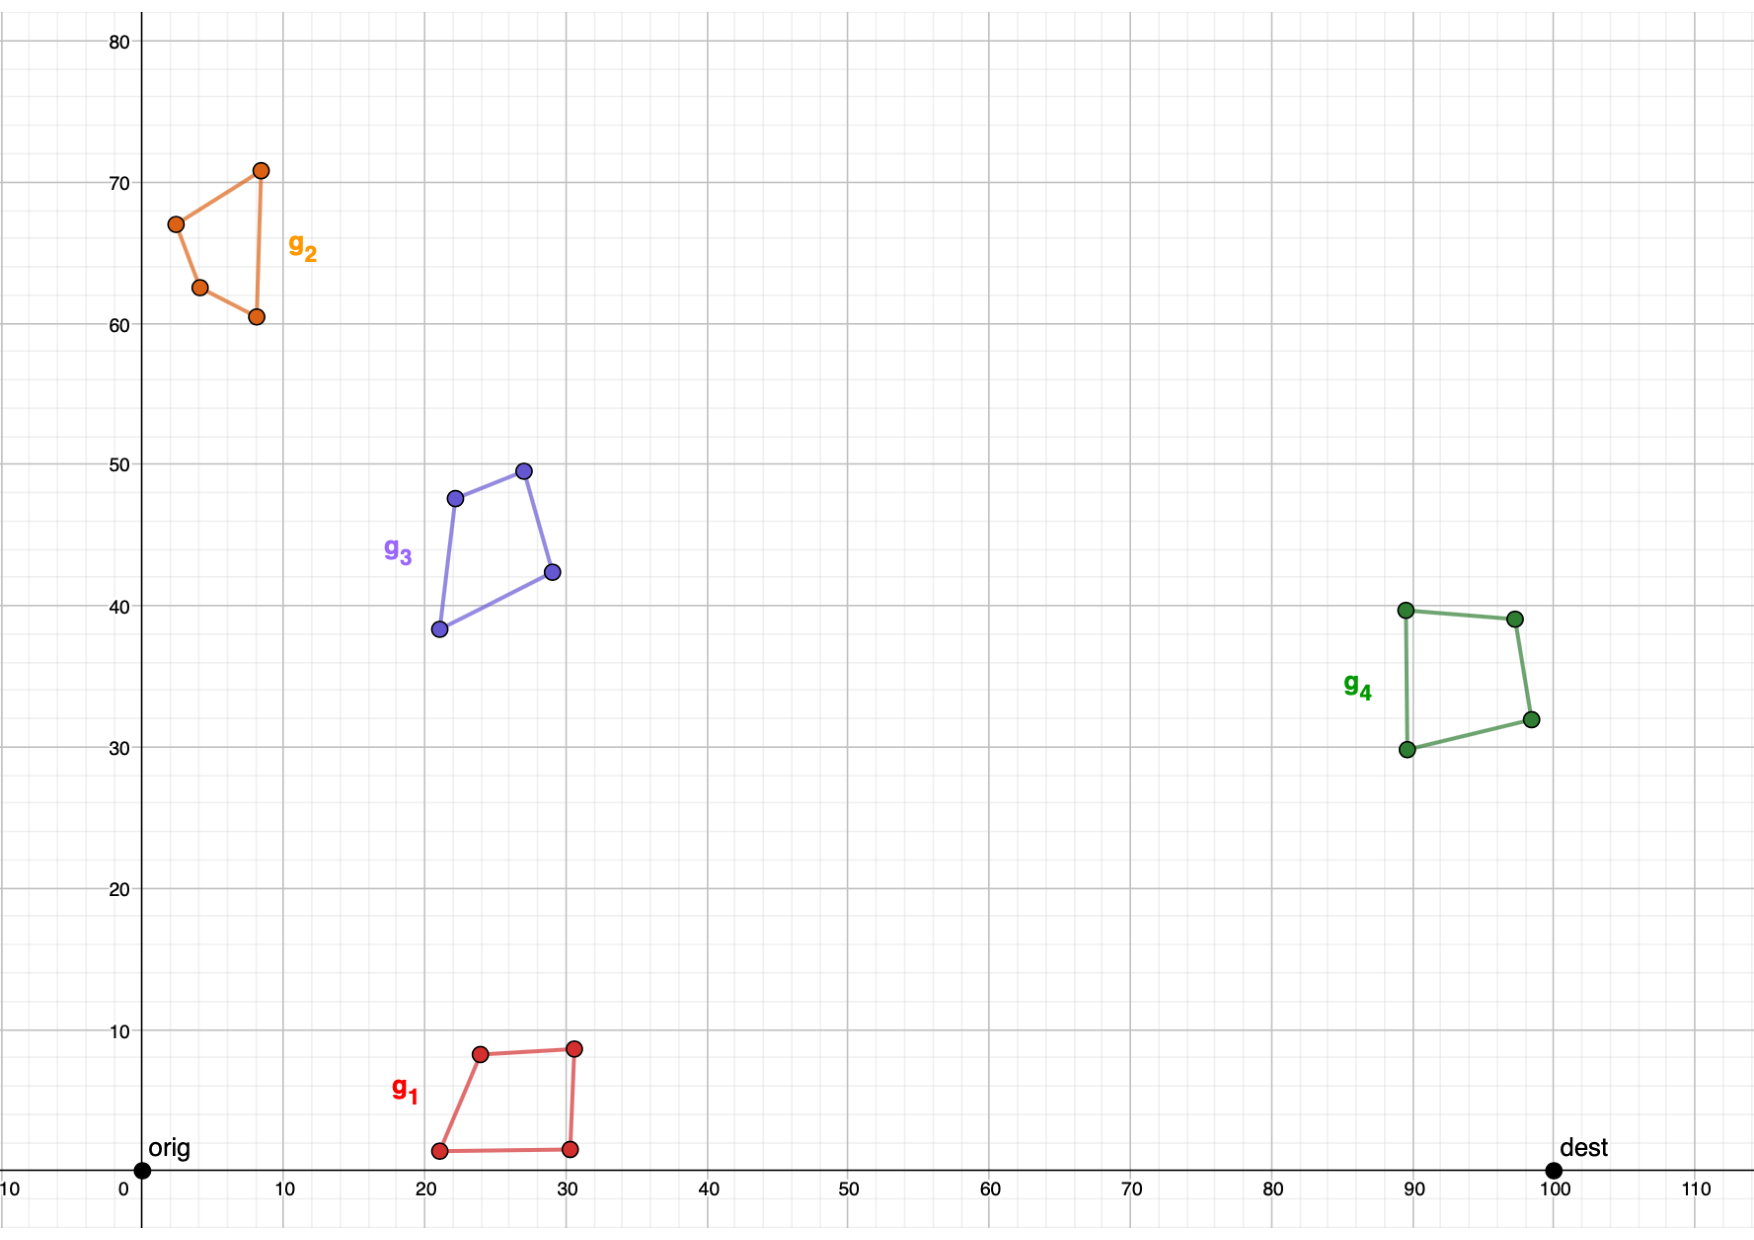
\includegraphics[width = 0.5\linewidth]{figures/example_new.pdf}
\caption{Illustrative example \label{fig:example1}}
\end{figure}

\noindent
Figure \ref{fig:example1} shows an illustrative example consisting of four target planar graphs ($g_1$, $g_2$, $g_3$ and $g_4$) to be visited. We assume that their visits must be performed by a fleet of two drones supported by a mothership whose path starts from the origin $(0,0)$ and ends on the destination point $(100,0)$.



\begin{figure}[h!]
    \centering
    \subfloat[\centering a]{{\includegraphics[width=4cm]{figures/example_tour_g1_Step1_new.png} }}%
    \qquad
    \subfloat[\centering b]{{\includegraphics[width=4cm]{figures/example_tour_g2_Step1_new.png} }}%
     \qquad
     \\
    \subfloat[\centering c]{{\includegraphics[width=4cm]{figures/example_tour_g3_Step1_new.png} }}%
    \qquad
    \subfloat[\centering d]{{\includegraphics[width=4cm]{figures/example_tour_g4_Step1_new.png} }}%
    \caption{STEP 1 for the illustrative example}%
    \label{fig:example2}%
\end{figure}

\noindent
Figure \ref{fig:example2} reports a zoom on each single target graph, showing the tours generated by STEP 1 of the matheuristic procedure. A pair of points representing retrieving and launching points,  together with an arrow pointing the direction followed by the drone according to the order in which the edges are visited, are depicted on each edge.

\begin{figure}[h!]
    \centering
    \subfloat[\centering a]{{\includegraphics[width=5cm]{figures/example_step2_new.png}}}%
    \qquad
    \subfloat[\centering b]{{\includegraphics[width=5cm]{figures/example_step3_new.png}}}%
        \caption{[a] STEP 2, [b] STEP 3 for the illustrative example}%
    \label{fig:example3}%
\end{figure}

\noindent
By applying STEP 2 to this illustrative example, we obtain three clusters, as shown in Figure \ref{fig:example3}[a]. One cluster contains graphs $g_1$ and $g_3$ (in lavender), while graph $g_2$ and $g_4$ represent distinct clusters. The computation of the reference points of these clusters, according \RE{to} STEP 3, produces the \RE{points $P_1$, $P_2$ and  $P_3$}, as shown in Figure  \ref{fig:example3}[b].
%Note that in this case the reference points for the two clusters containing\CV{,} respectively $g_2$ and $g_4$ coincide, and thus we have only two distinct reference points for the three clusters.

%\JP{*** With 3 clusters we should have three reference points, am I confused? ***}

\begin{figure}[h!]
    \centering
    \subfloat[\centering a]{{\includegraphics[width=5cm]{figures/example_step4_new.png} }}%
    \qquad
    \subfloat[\centering b]{{\includegraphics[width=5cm]{figures/example_step5_new.png} }}%
        \caption{[a] STEP 4, [b] STEP 5 for the illustrative example}%
    \label{fig:example4}%
\end{figure}

\noindent
STEP 4 of the matheuristic procedure generates the tour of the mothership along the origin point, \RE{$P_1$, $P_2$, $P_3$ and the destination point}, as shown in Figure \ref{fig:example4}[a]. This tour returns also the order in which the clusters are visited (and thus, also the order of visit\RE{s} to the target graphs) and this permits to set the values of the variables $u^{e_{g}o}$ and $v^{e_{g}o}$ of the \AMD\space model.\\
\noindent 
By providing the initial partial solution obtained by the values of the variables $u^{e_{g}o}$ and $v^{e_{g}o}$, STEP 5 solves the \AMD\space model and returns the final feasible solution shown in Figure \ref{fig:example4}[b]. From it\RE{,} we can observe that the sequence of visit\RE{s} of the target graphs does not change with respect to the one provided by STEP 4. The fleet of two drones first visits \RE{the} graphs $g_1$ and $g_3$ starting from the launching point $x^1_L$. Then, both drones are retrieved by the mothership at \RE{the} point $x^1_R$. The mothership moves to the point $x^2_L$  where one drone is launched for visiting graph $g_2$. Then the mothership reaches \RE{the} point $x^2_R$ to retrieve the drone and from the same point it launches the other drone for visiting graph $g_4$. Then, this drone is retrieved by the mothership at point $x^3_R$ before moving to the final destination point.


\begin{figure}[h!]
    \centering
    \subfloat[\centering a]{{\includegraphics[width=5cm]{figures/example_final-g1_g3.png}}}%
    \qquad
    \subfloat[\centering b]{{\includegraphics[width=5cm]{figures/example_final-g2.png} }}%
     \qquad
    \subfloat[\centering c]{{\includegraphics[width=5cm]{figures/example_final-g4.png} }}%
    \caption{Zoom on the tour on each target graph provided by STEP 5}%
    \label{fig:example5}%
\end{figure}

\noindent 
Focusing on each single target graph, Figure \ref{fig:example5} shows the zoom on the tours followed by the drones. For example, Figure \ref{fig:example5}[a] reports the one performed by the drone that visits \RE{the} graph $g_1$ \RE{(in pink) and the drone that visits the graph $g_3$ (in sky blue)}. \RE{Both drones start from the mothership at point $x^1_L$ that is the $orig$. One drone first visits the segment $\overline{R^1_1L^1_1}$ of the graph $g_1$, while the other one starts the visit of the graph $g_3$ by traversing the segment $\overline{R^3_1L^3_1}$. From point $L^1_1$ the first drone moves to the second visited edge of the graph $g_1$ by traversing the segment $\overline{R^2_1L^2_1}$. Then, it moves to the third visited edge of graph $g_1$, by flying over the segment $\overline{R^3_1L^3_1}$. From point $R^4_1$ the drone starts the visit of the last edge of graph $g_1$ up to point $L^4_1$. 
Finally, the drone leaves the graph $g_1$ at this latter point and it is retrieved by the mothership at the point $x^1_R$. Similarly, the second drone, that visits the graph $g_3$, after traversing the segment $\overline{R^1_3L^1_3}$, moves to the second visited edge of the same graph and traverses the segment $\overline{R^2_3L^2_3}$. Then, it flies to the third visited edge, by traversing the segment $\overline{R^3_3L^3_3}$. Finally it moves to the last visited edge of the graph $g_3$, by flying over the segment $\overline{R^4_3L^4_3}$. The drone leaves the graph $g_3$ at point $L^4_3$ and reaches the mothership at point $x_R^1$.} 
Note that in this example the drones do not visit the full 100\% of each \RE{graph edge}, but only the half of each one of them.

\bigskip
\noindent
The reader may notice that the above algorithm can be also used to generate solutions for the \RE{partial overlapping model presented in Section \ref{amdasyn} since any solution of the \AMDCO\xspace model is also feasible for the \AMDPO\xspace one as shown in \JP{Theorem \ref{th:relaxation}.}}

\begin{comment}
\JP{ \textbf{\noindent ***   NOT CLEAR THAT WE SHOULD INCLUDE THIS PART  (JUSTO: dixit) ***}
\bigskip

\noindent
As we already explained in Section \ref{amdasyn}, we also studied a variant of the \AMD\space model in which the mothership can launch and retrieve a drone in different stages. We \CV{also} designed a matheuristic (also) for this case with similar steps to the one previously presented.
The idea of this procedure is first solving the model with only one available drone (see \cite{art:Amorosi2021}) to determine the optimal launching/rendezvous points associated with each target graph and the corresponding minimum length of the mothership tour.
Then, a clustering procedure, like the one adopted in the matheuristic proposed for the synchronous case, is performed.
After that, the \AMD\space model without synchronization is solved (on) \CV{for} each cluster\CV{,} setting the launching point of the first cluster equal to the origin. Then the last retrieving point (so) \CV{determined} is set as \CV{the} launching point of the next cluster\CV{,} and so on. From the solution obtained for each cluster\CV{,} the total length of the mothership tour is computed as the sum of the partial lengths of each tour associated with each cluster. The same procedure is repeated by starting the clustering procedure with different random seed.\\
In the following, we present the (pseudo-code) \CV{pseudocode} of this algorithm:

\begin{itemize} 
\item[STEP 1] (Launching/rendezvous points)
Solve the AMDRPG model and let $x_L^g$ and $x_R^g \forall g \in \mathcal{G}$ the associated optimal launching/rendezvous points and let $L$ be the associated minimum length of the mothership tour.  
\item[STEP 2] (Clustering procedure)
Initialization: define one cluster for each target graph and set $nit=1$ \\
Select randomly two clusters $C_i$ and $C_j$ (where $i<j$).\\
Check if the number of graphs belonging to the union of $C_i$ and $C_j$ is less than or equal to the number of available drones $n_D$.\\
If this condition is satisfied:\\
search for the point $C$ satisfying the following \RE{\sout{capacity} endurance} constraint:
$$
\frac{[d(C, R^{e_g}) + C^{e_{g}e^{'}_{g}} + d(C,L^{e^{'}_{g}})]}{v_D} \leq cap \:\: \forall R^{e_g}, L^{e^{'}_{g}} \in C_i, \:\: C_j
$$
If such a point exists, merge the two clusters and assign to the resulting cluster so obtained the label $C_i$.\\

\item[STEP 3](Launch/rendezvous point exchanges)
Set $i=1$ and $x_L=orig$\\
For each cluster $C_i$ generated at STEP 2:\\
- solve the \AMD\space model with first launching point equal to $x_L$.\\
- let $x_R$ be the last rendezvous point associated with the cluster under analysis, set $x_L = x_R$.\\
Let $L'$ be the associated minimum length of the mothership tour computed as sum of the partial lengths of the tours associated with the clusters.\\
If $L' < L$ update the solution.\\
Set $nit=nit+1$.\\
Repeat STEP 2 and STEP 3 while $nit < maxit$
\end{itemize}
}
\end{comment}



\section{A Matheuristic for the Mothership-Drone Routing Problem with Graphs}\label{Math}
\noindent
This section is devoted to present our matheuristic approach to address the solution of the \AMD. Our motivation comes from the fact that the exact solution of the models presented in Section \ref{Form} is highly time demanding. Alternatively, the matheuristic provides \RE{a} good quality solution in limited computing times.\\
\noindent
%\JP{First, we focus on the synchronized case in which each drone that is used must be launched and retrieved in the same stage.}
The basic idea of the algorithm is to determine the route that a drone should perform for visiting each graph $g \in \mathcal{G}$, and thus the entry and exit points $L^{e_{g}}$ and $R^{e^{'}_{g}}$ for each graph.
Sequentially, a clustering procedure on the target graphs is applied \RE{to} compute the route of the mothership via their reference points and the origin/destination points.
The clustering procedure is based on a random selection of the initial target graphs and for this reason it is repeated a number of times to consider different cluster structures. At each iteration\RE{,} the new clusters are evaluated by computing the cost of the route visiting their reference points and the origin/destination points. 
The route of minimum length, computed on the reference points of the cluster generated by this iterative procedure, is used to set the values of the binary variables $u^{e_go}$ and $v^{e_go}$, that determines the order of visits to the graphs. Finally, these variables are provided as an initial partial solution to the \AMDCO\xspace model to produce a complete feasible solution.\\
\RE{Algorithm \ref{alg:math}} reports the pseudocode of this algorithm.

\begin{algorithm}
\caption{Matheuristic algorithm for \ref{AMMDRPG}}\label{alg:math}
\KwData{$\mathcal{G}$, $|\mathcal{D}|$, $N_D$, $v_D$, $maxit$ (maximum number of iterations to perform the clustering procedure), $maxseed$ (maximum number of the clustering procedure repetitions)}

STEP 1 (First entry and last exit points for each target graph)\\
\begin{algorithmic}
\State For each target graph $g \in \mathcal{G}$, compute the route:\\
 $ L^{e_{g}} \gets \mbox{entry point on $g$ closest to the origin}$\\
 $R^{e^{'}_{g}} \gets \mbox{exit point from $g$ closest to the origin}$\\
 $\mathcal L(e_{g}, e^{'}_{g}) \gets \mbox{route length}$
\end{algorithmic}
STEP 2 (Clustering procedure)
\begin{algorithmic}
\State $it \gets 1$
\State $nit \gets 1$
\State For each target graph $g \in \mathcal{G}$:\;
$K_g \gets g$ \Comment{one cluster for each target graph}\\
\While{$nit < maxit$}{
\State Select randomly two clusters $K_i$ and $K_j$ ($i < j$)\\
\If{$| K_i \cup K_j | < |\mathcal{D}|$}
{
\State Search for point $P$ satisfying the following endurance constraint:\\
\begin{equation}
\frac{d(P, R^{e_g}) + \mathcal L(e_{g}, e^{'}_{g}) + d(L^{e^{'}_{g}}, P)}{v_D} \leq N_D, \quad \forall R^{e_g}, L^{e^{'}_{g}} \in K_i, \:\: K_j. \label{eq:endurance_math}
\end{equation}
\If{$P \:\: \exists$}{\State $K_i \gets K_i \cup K_j$}
}
\State $nit \gets nit +1$
}
$\mathcal K \gets \mbox{set of clusters}$
\end{algorithmic}
STEP 3 (Computation of Reference Points) 
\begin{algorithmic}
\State For each cluster $K_i \in \mathcal K$\;
compute a reference point $P_i$ by solving the following minimization problem:
$$
\min \sum_{K_i \in \mathcal K}( \|P_i - origin\| + \|P_i - dest \|) + \sum_{g \in K_i: K_i \in \mathcal K} (\|P_i - R^{e_g} \| + \| P_i - L^{e'_g}\|) + \sum_{K_i, K_j \in \mathcal K: i \neq j} \|P_i - P_j\|
$$
subject to (\ref{eq:endurance_math}).
\end{algorithmic}
STEP 4 (Order of visits to the graphs: route via the reference points and the origin/destination points)
\begin{algorithmic}
\State Compute the TSP of the mothership among the reference points $P_i$ of the clusters\\
\State \CV{$\mathcal L(TSP) \gets \mbox{TSP length}$} [This update is performed only if $\mathcal L(TSP)$ decreases with respect to the previous iteration $it - 1$]
\State $it \gets it+1$\\
\eIf{$it < maxseed$}{go to STEP 2}{go to STEP 5}
\end{algorithmic}
STEP 5 (Solution of the \AMD\xspace model by fixing an initial partial solution)
\begin{algorithmic}
\State Set the initial values of the binary variables $u^{e_{g}o}$ and $v^{e_{g}o}$ and solve the model \CV{\AMD}\xspace to obtain a feasible solution.
\end{algorithmic}
\KwResult{Feasible solution for \CV{\ref{AMMDRPG}}}
\end{algorithm}

\begin{comment}
\begin{itemize} 
\item[STEP 1] (First entry and last exit points for each target graph)\\
Compute the route \CV{for} (on) each target graph $g \in \mathcal{G}$.
Let $L^{e_{g}}$ and $R^{e^{'}_{g}}$ be the pair of entry and exit points on $g$ closest to the origin and let  $\mathcal L(e_{g}, e^{'}_{g})$ be the associated length computed as the sum of the distances travelled by the drone to visit the graph $g$, excluding the distance between $L^{e_{g}}$ and $R^{e^{'}_{g}}$.
\item[STEP 2] (Clustering procedure)\\
Initialization: set $it=1$, define one cluster for each target graph and set $nit=1$. \\
Select randomly two clusters $K_i$ and $K_j$ (where $i<j$).\\
Check if the number of graphs belonging to the union of $K_i$ and $K_j$ is less than the number of available drones $n_D$.\\
If this condition is satisfied:\\
search for point $P$ satisfying the following \RE{\sout{endurance} endurance} constraint:
$$
\frac{d(P, R^{e_g}) + \mathcal L(e_{g}, e^{'}_{g}) + d(L^{e^{'}_{g}}, P)}{v_D} \leq N^d, \quad \forall R^{e_g}, L^{e^{'}_{g}} \in K_i, \:\: K_j.
$$
If such a point exists, merge the two clusters and label the new one as $K_i$.\\
Set $nit=nit+1$.\\
Repeat the same procedure on the new cluster structure while $nit < maxit$.
\item[STEP 3] (Computation of Reference Points) 
%\JP{This step is not well-defined: The term centroid defines exactly the points we should use another term that allows to minimize something!!!} \\
% Compute the centroids of the clusters generated at STEP 2, by minimizing the distance between them and the origin always imposing that the \RE{\sout{endurance} endurance} constraint is satisfied.
Compute a reference point for each cluster generated (at) \CV{in} STEP 2. This computation seeks for the minimization of the distance between each pair of reference points and the distance between them and the origin, always imposing that the \eqref{CAP} constraint is satisfied.



\item [STEP 4] (Setting the order of visits to the  graphs: route via the reference points and the origin/destination points) \\
Compute the TSP of the mothership among the reference points of the clusters and let $\mathcal L(TSP)$ be the associated length.\\
Set $it=it+1$.\\
if(it< maxseed) go to STEP 2\\
else go to STEP 5
\item [STEP 5] (Solution of the \AMD\space model fixing an initial partial solution)\\
Set the values of the binary variables $u^{e_{g}td}$ and $v^{e_{g}td}$ and solve the model \AMD\, to obtain a feasible solution.
\end{itemize}
\end{comment}
\noindent
%}



\begin{figure}[h]
\centering
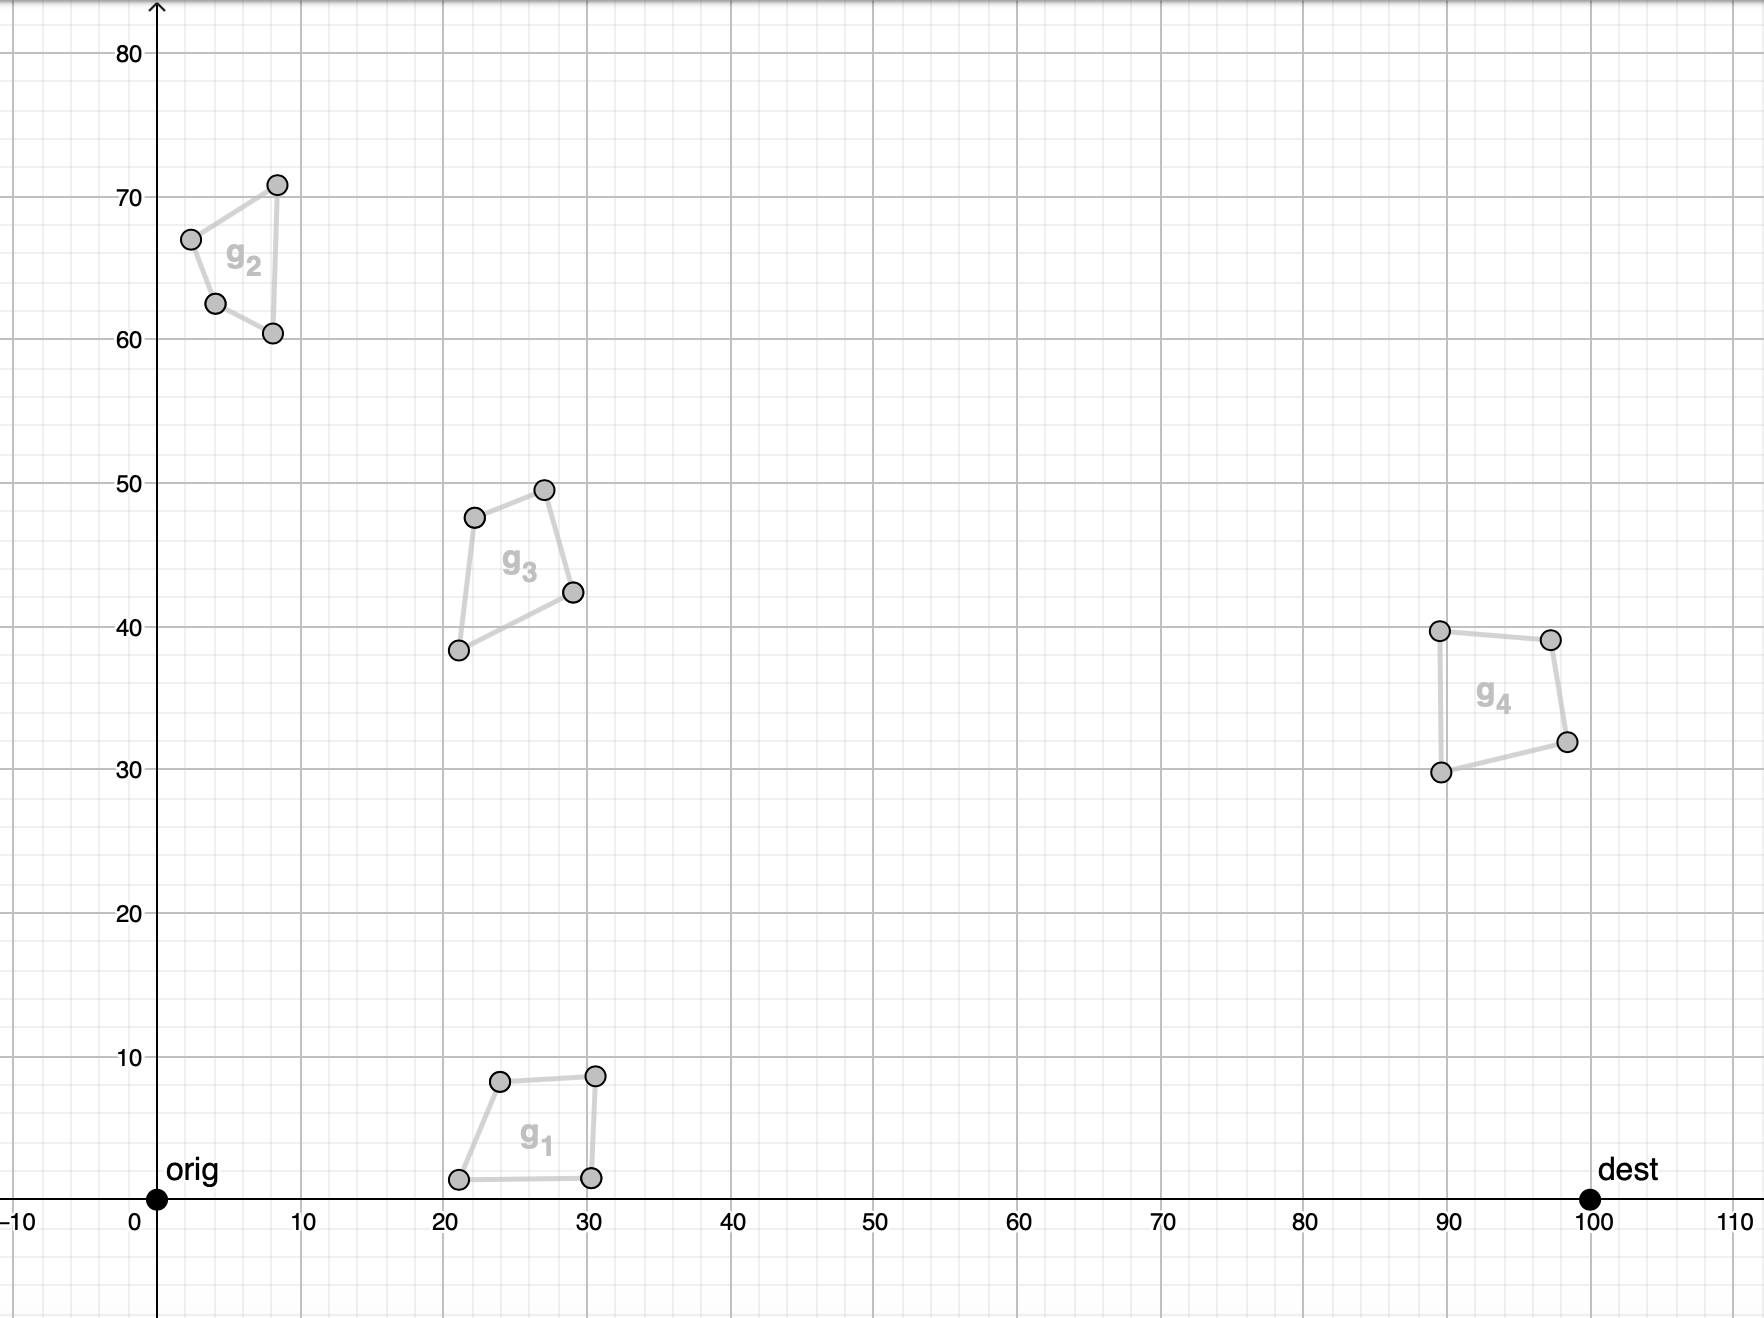
\includegraphics[width = 0.5\linewidth]{example_new_gray.png}
\caption{Illustrative example \label{fig:example1}}
\end{figure}

\noindent
Figure \ref{fig:example1} shows an illustrative example consisting of four target planar graphs ($g_1$, $g_2$, $g_3$ and $g_4$) to be visited. We assume that their visits must be performed by a fleet of two drones supported by a mothership whose path starts from the origin $(0,0)$ and ends on the destination point $(100,0)$.



\begin{figure}[h!]
	\centering
    \begin{subfigure}[b]{.35\textwidth}
    	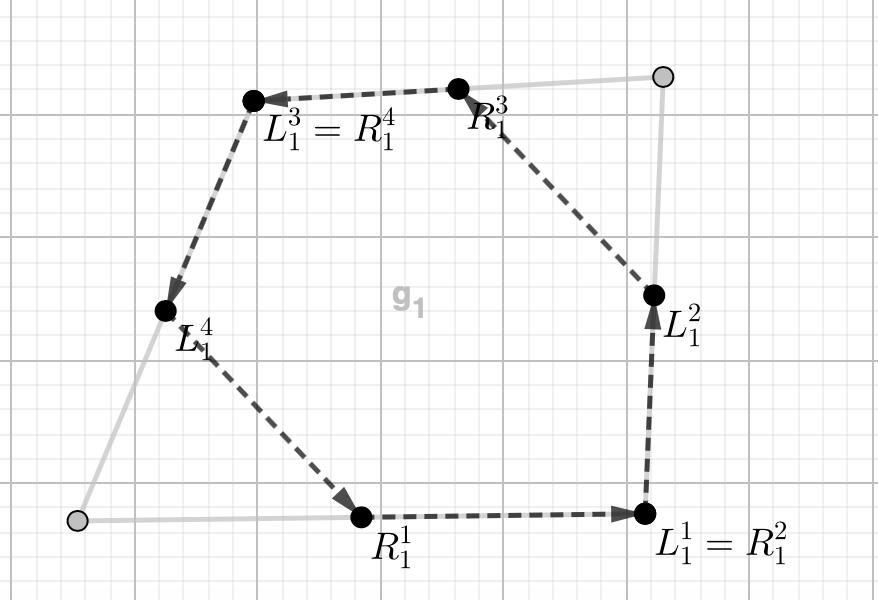
\includegraphics[width=\textwidth]{example_tour_g1_Step1_new_gray.png}
    	\caption{}
    \end{subfigure}
	\begin{subfigure}[b]{.35\textwidth}
		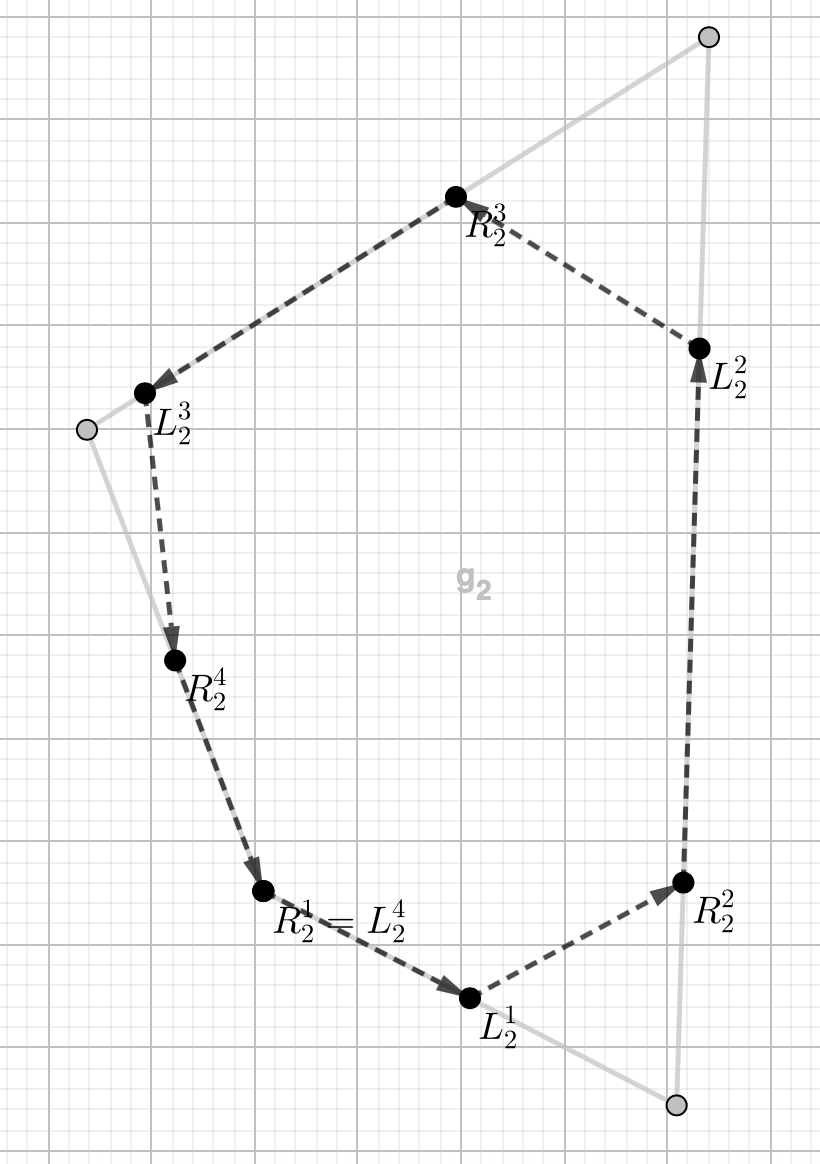
\includegraphics[width=\textwidth]{example_tour_g2_Step1_new_gray.png}
		\caption{}
	\end{subfigure}
    \begin{subfigure}[b]{.35\textwidth}
		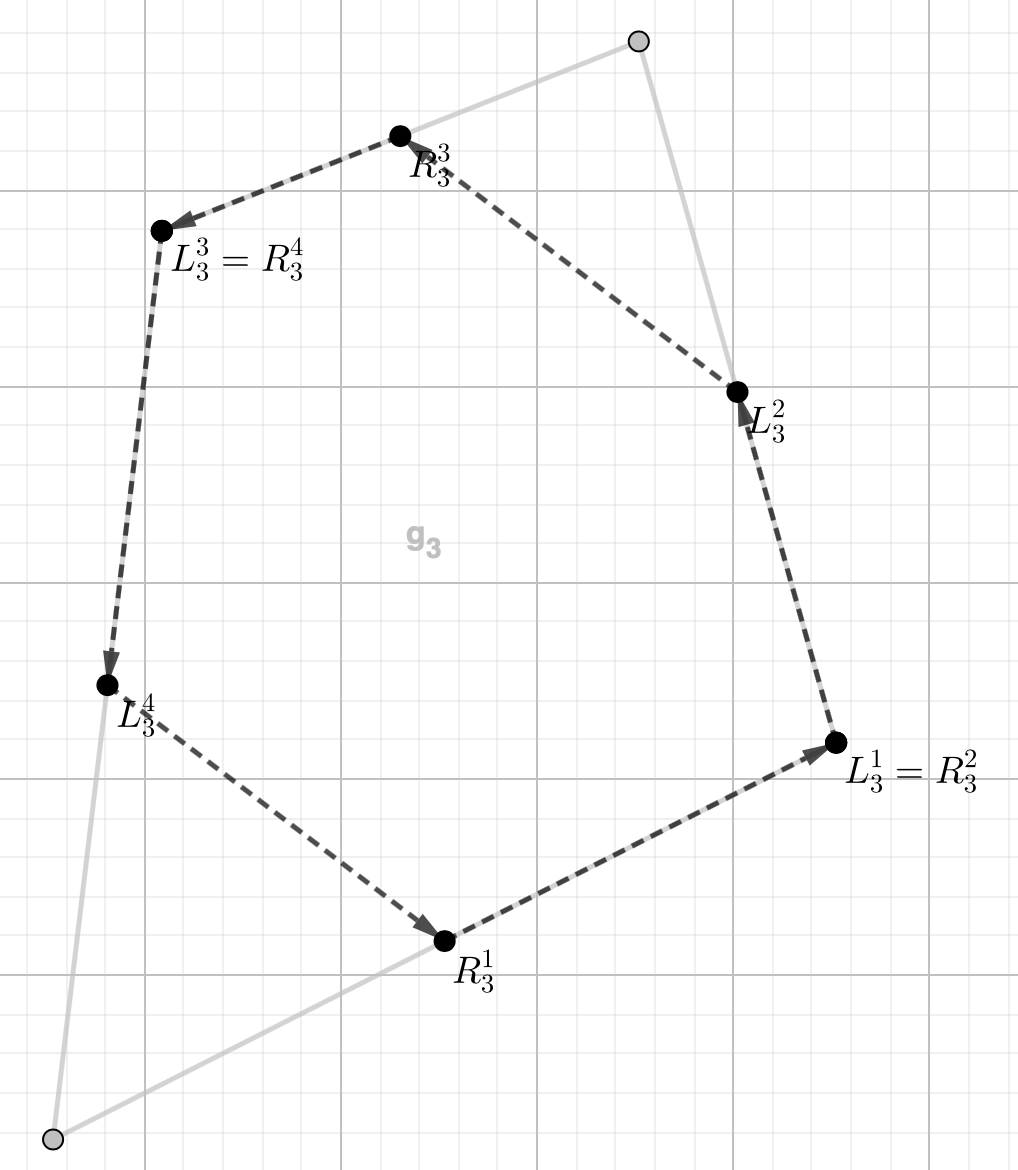
\includegraphics[width=\textwidth]{example_tour_g3_Step1_new_gray.png}
		\caption{}
	\end{subfigure}
	\begin{subfigure}[b]{.35\textwidth}
		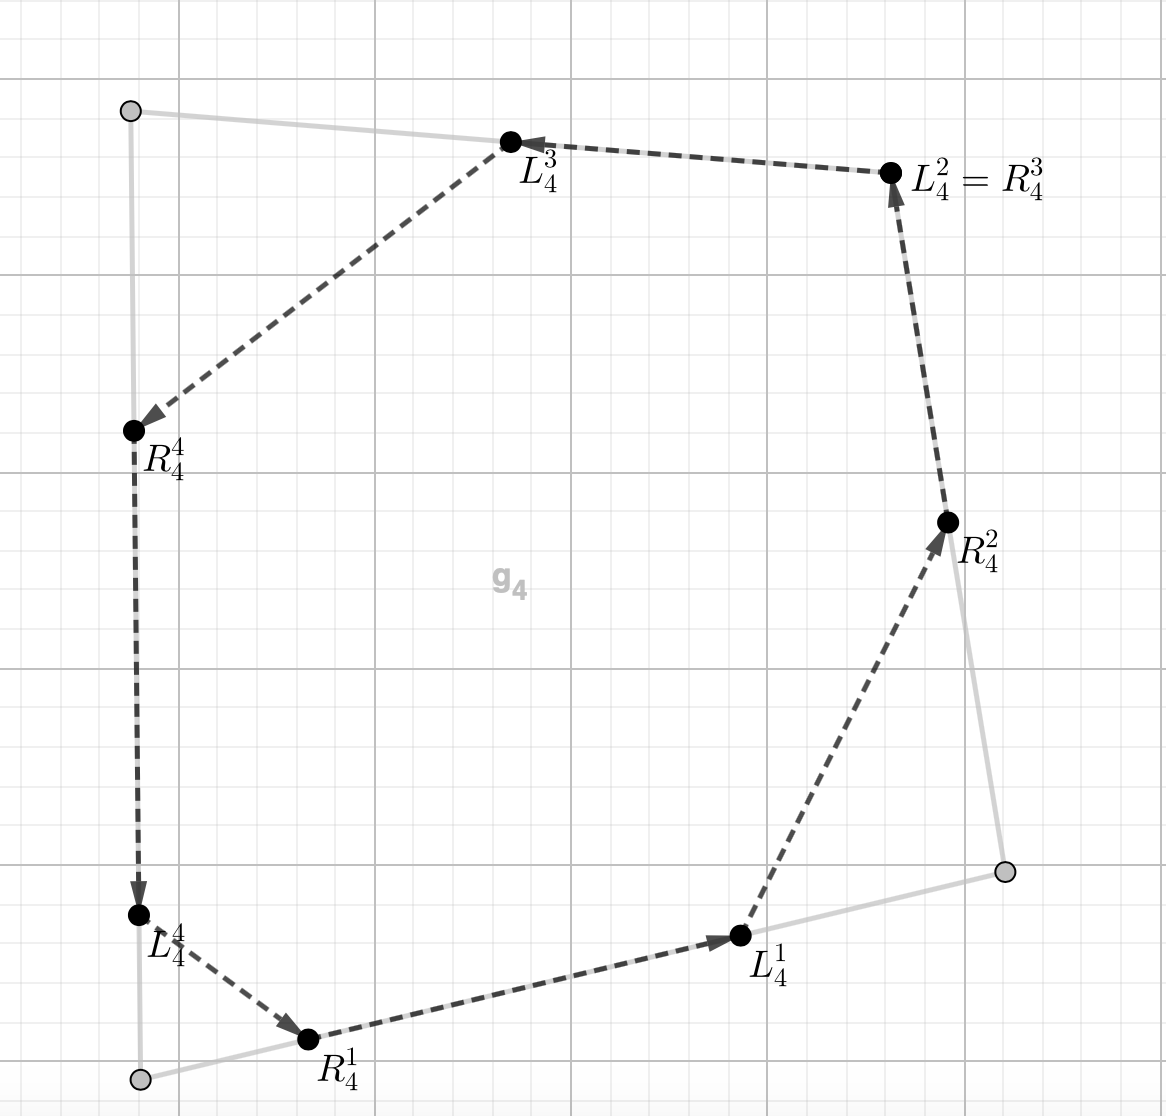
\includegraphics[width=\textwidth]{example_tour_g4_Step1_new_gray.png}
		\caption{}
	\end{subfigure}
    \caption{STEP 1 for the illustrative example}%
    \label{fig:example2}%
\end{figure}

%\begin{figure}
%    \subfloat[\centering a]{{\includegraphics[width=4cm]{example_tour_g1_Step1_new.png} }}%
%    \qquad
%    \subfloat[\centering b]{{\includegraphics[width=4cm]{example_tour_g2_Step1_new.png} }}%
%     \qquad
%     \\
%    \subfloat[\centering c]{{\includegraphics[width=4cm]{example_tour_g3_Step1_new.png} }}%
%    \qquad
%    \subfloat[\centering d]{{\includegraphics[width=4cm]{example_tour_g4_Step1_new.png} }}%
%    \caption{STEP 1 for the illustrative example}%
%    \label{fig:example2}%
%\end{figure}

\noindent
Figure \ref{fig:example2} reports a zoom on each single target graph, showing the tours generated by STEP 1 of the matheuristic procedure. A pair of points representing retrieving and launching points,  together with an arrow pointing the direction followed by the drone according to the order in which the edges are visited, are depicted on each edge.

\begin{figure}[h!]
    \centering
    \begin{subfigure}[b]{.4\textwidth}
    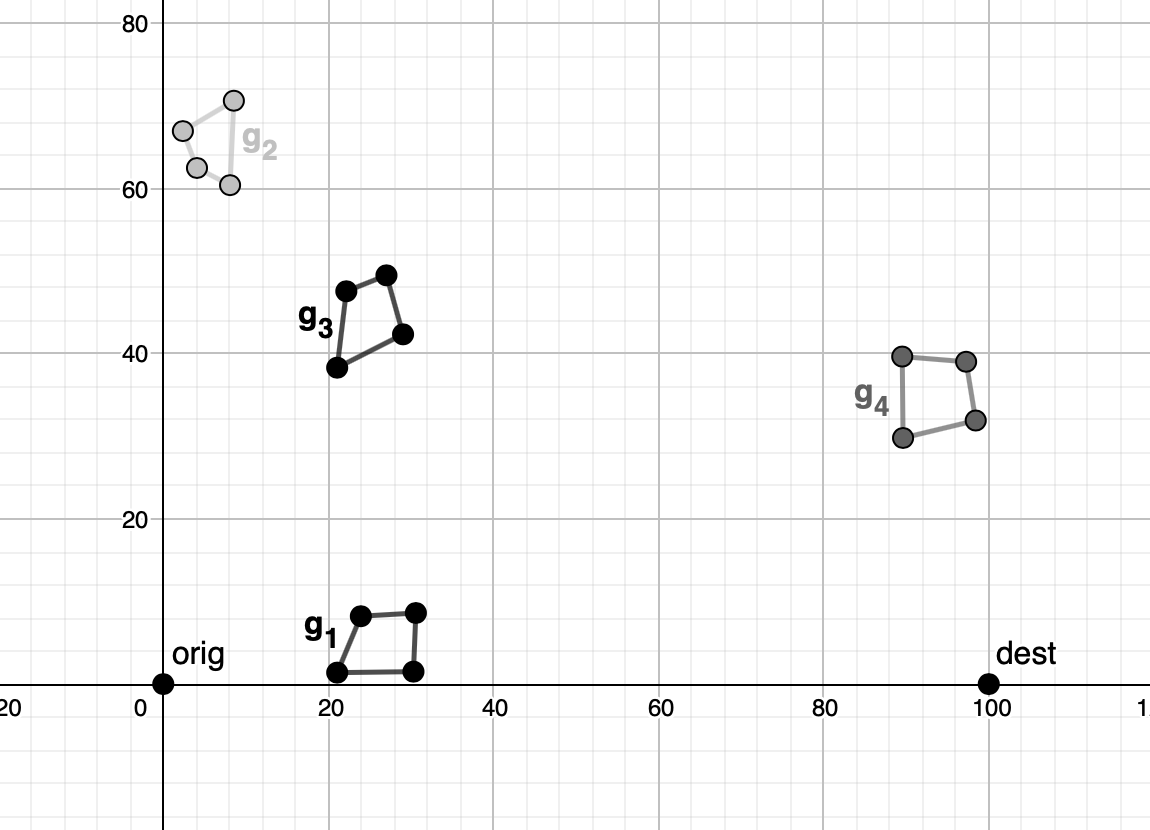
\includegraphics[width=\textwidth]{example_step2_new_gray.png}
    \caption{}%
	\end{subfigure}
	\begin{subfigure}[b]{.4\textwidth}
	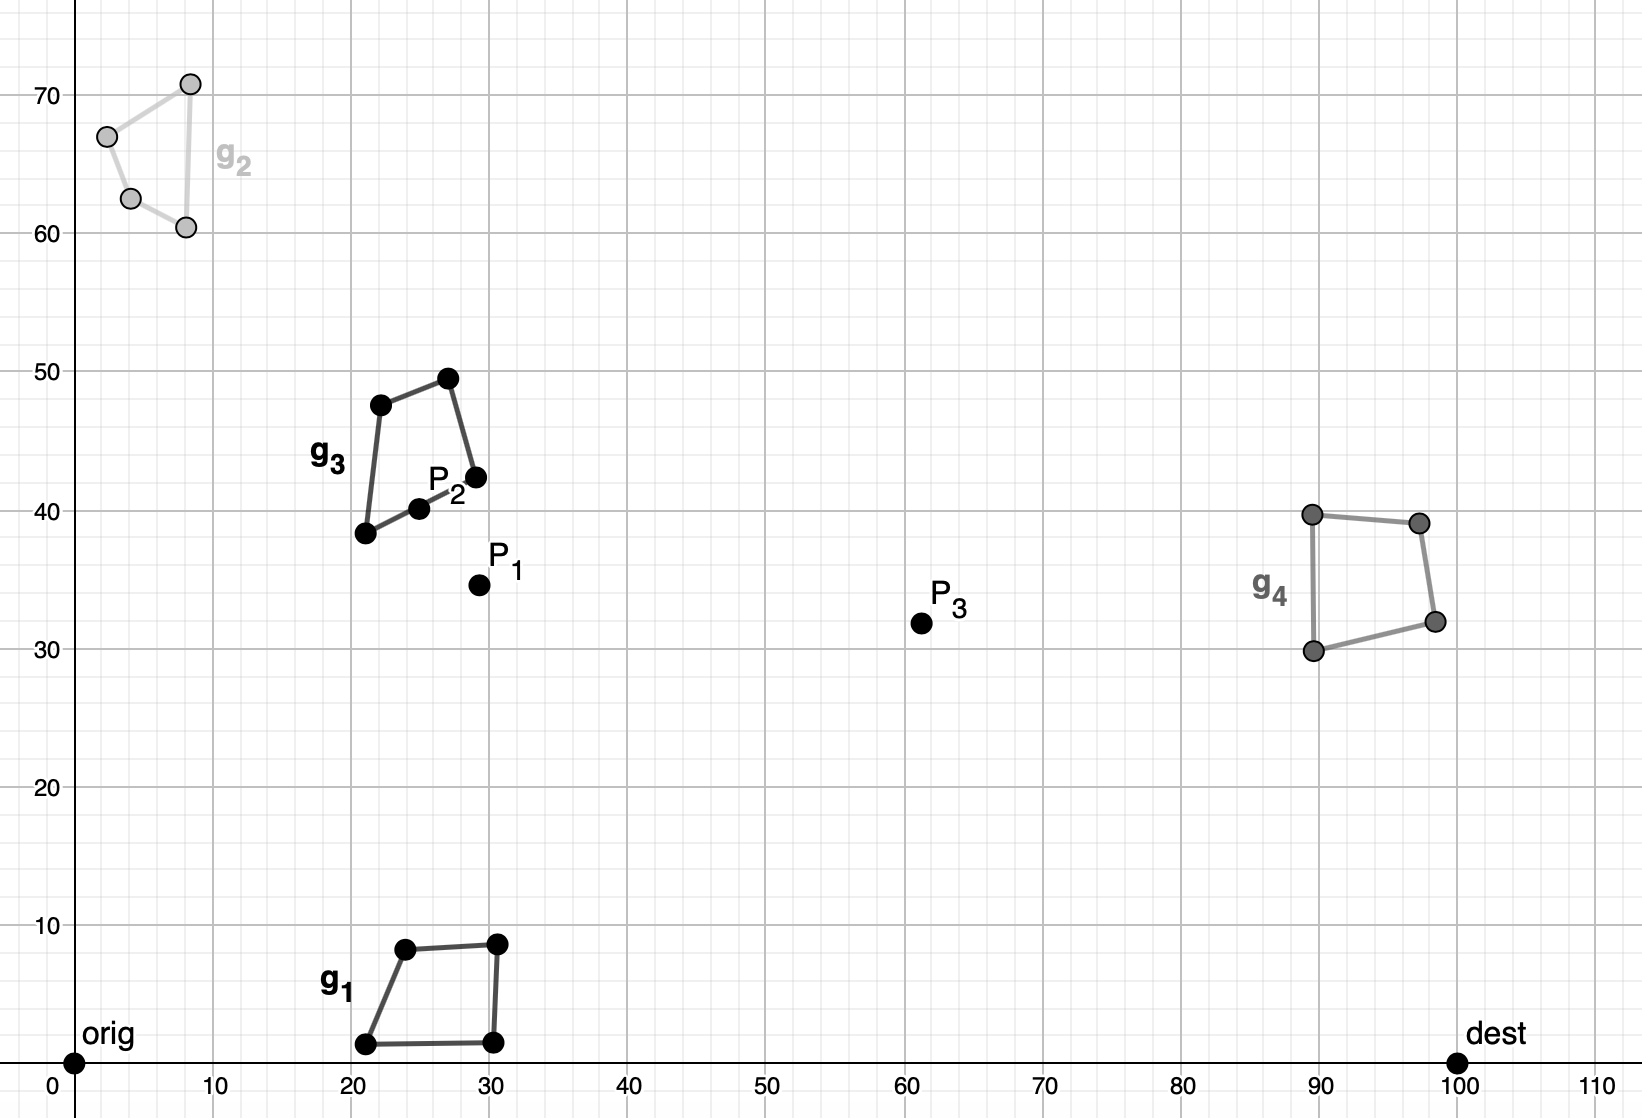
\includegraphics[width=\textwidth]{example_step3_new_gray.png}
	\caption{}%
	\end{subfigure}
    \caption{(a) STEP 2, (b) STEP 3 for the illustrative example}%
    \label{fig:example3}%
\end{figure}


%\begin{figure}[h!]
%    \centering
%    \subfloat[\centering a]{{\includegraphics[width=5cm]{example_step2_new.png}}}%
%    \qquad
%    \subfloat[\centering b]{{\includegraphics[width=5cm]{example_step3_new.png}}}%
%        \caption{[a] STEP 2, [b] STEP 3 for the illustrative example}%
%    \label{fig:example3}%
%\end{figure}

\noindent
By applying STEP 2 to this illustrative example, we obtain three clusters, as shown in Figure \ref{fig:example3}[a]. One cluster contains graphs $g_1$ and $g_3$ (in lavender), while graph $g_2$ and $g_4$ represent distinct clusters. The computation of the reference points of these clusters, according \RE{to} STEP 3, produces the \RE{points $P_1$, $P_2$ and  $P_3$}, as shown in Figure  \ref{fig:example3}[b].
%Note that in this case the reference points for the two clusters containing\CV{,} respectively $g_2$ and $g_4$ coincide, and thus we have only two distinct reference points for the three clusters.

%\JP{*** With 3 clusters we should have three reference points, am I confused? ***}

\begin{figure}[h!]
    \centering
    \begin{subfigure}[b]{0.4\textwidth}
    	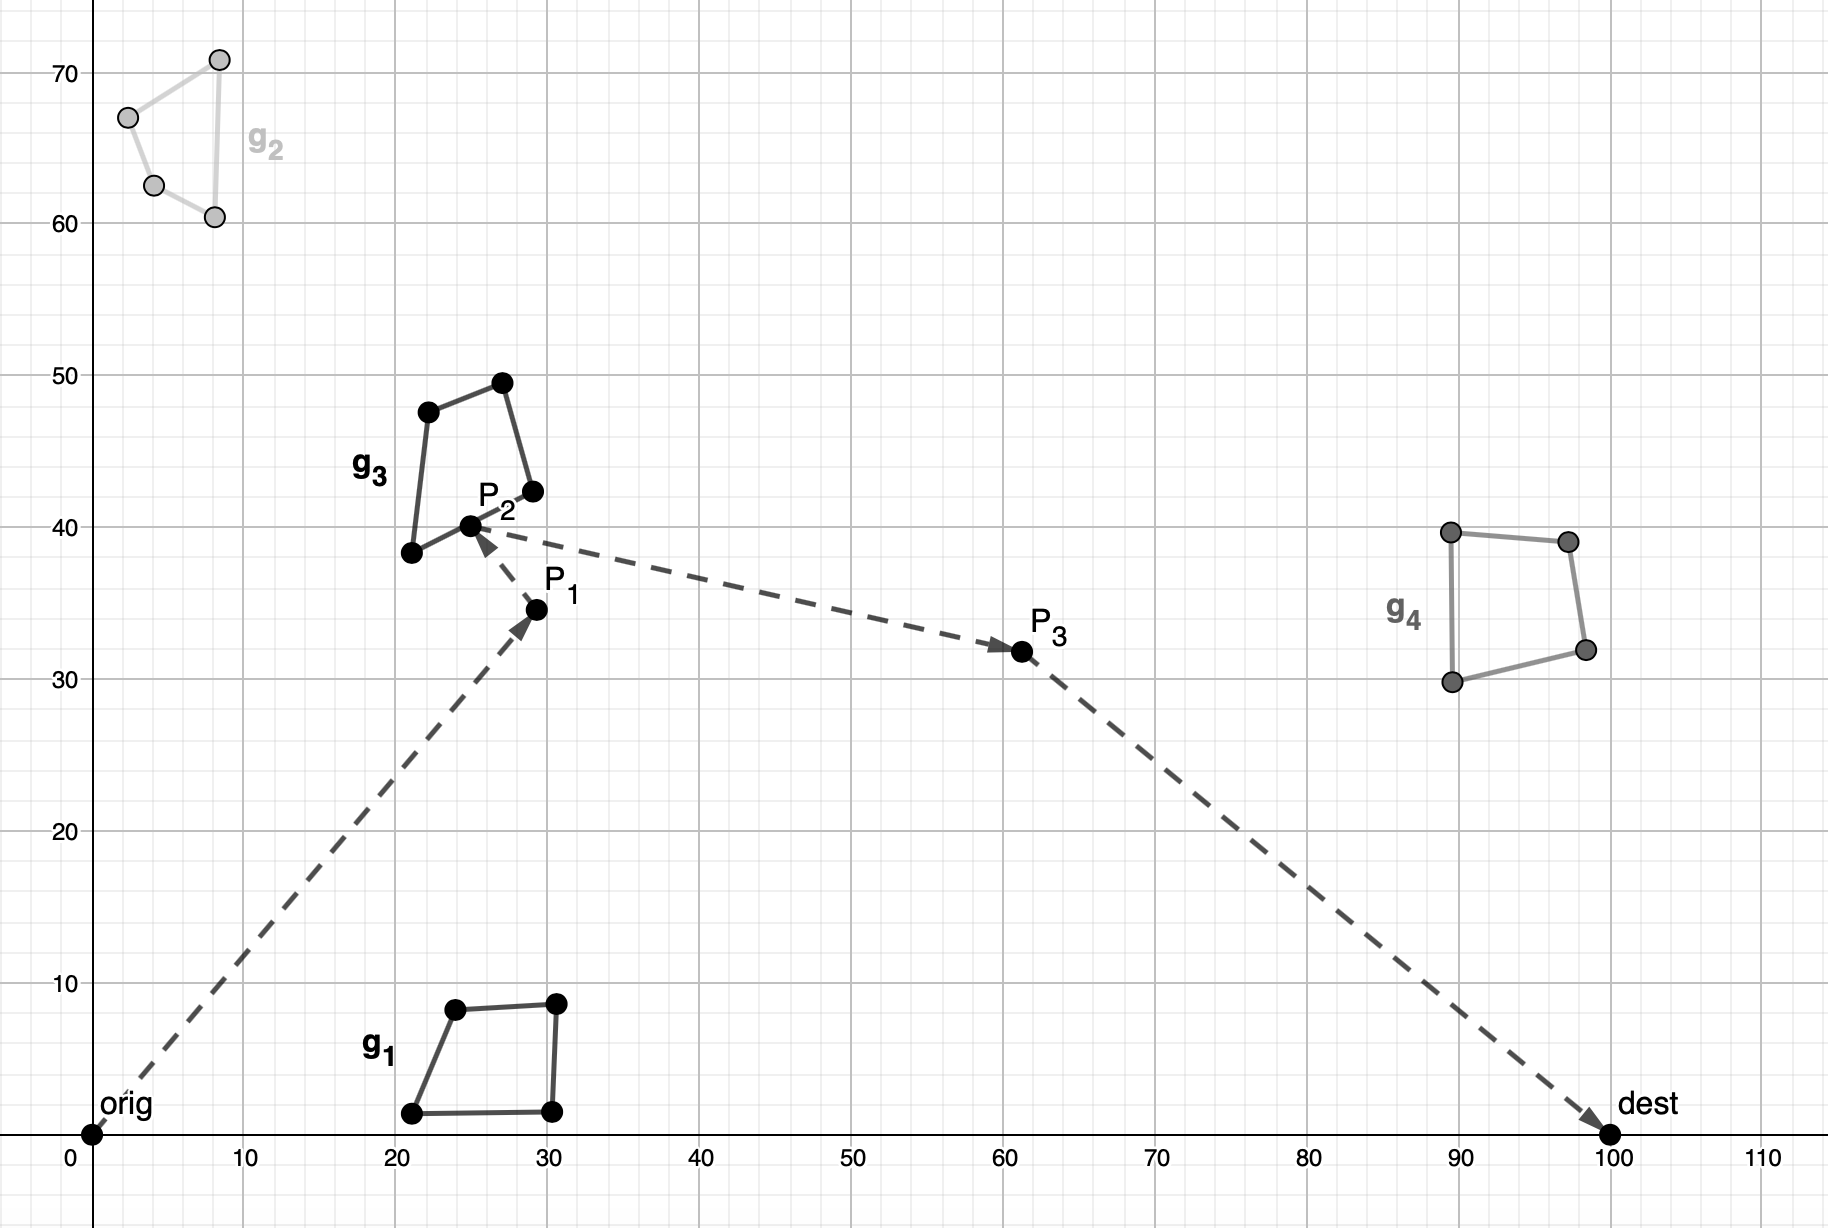
\includegraphics[width=\textwidth]{example_step4_new_gray.png}
		\caption{}%
    \end{subfigure}
	\begin{subfigure}[b]{0.4\textwidth}
		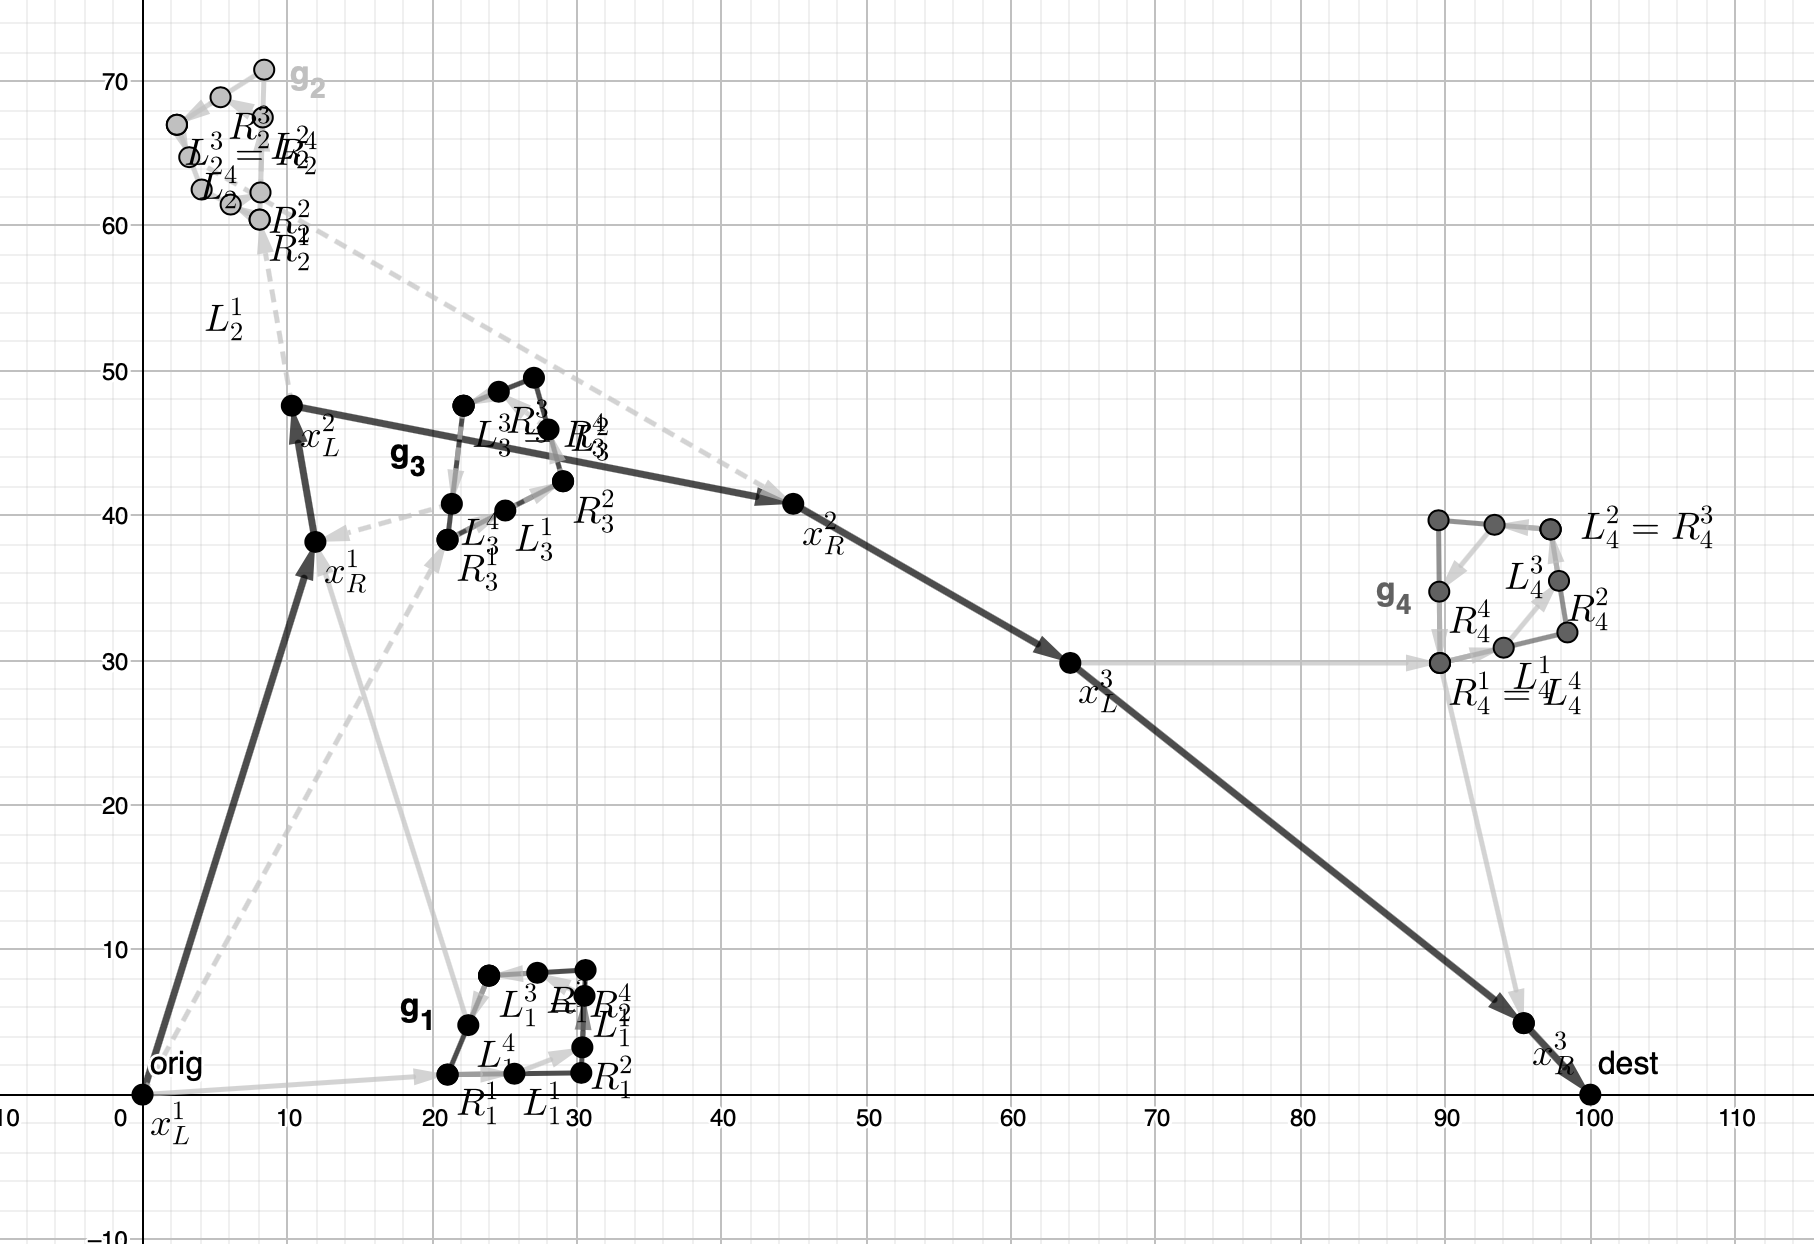
\includegraphics[width=\textwidth]{example_step5_new_gray.png}
		\caption{}
	\end{subfigure}%
    \caption{(a) STEP 4, (b) STEP 5 for the illustrative example}%
    \label{fig:example4}%
\end{figure}

%\begin{figure}[h!]
%    \centering
%    \subfloat[\centering a]{{\includegraphics[width=5cm]{example_step4_new.png} }}%
%    \qquad
%    \subfloat[\centering b]{{\includegraphics[width=5cm]{example_step5_new.png} }}%
%        \caption{[a] STEP 4, [b] STEP 5 for the illustrative example}%
%    \label{fig:example4}%
%\end{figure}

\noindent
STEP 4 of the matheuristic procedure generates the tour of the mothership along the origin point, \RE{$P_1$, $P_2$, $P_3$ and the destination point}, as shown in Figure \ref{fig:example4}[a]. This tour returns also the order in which the clusters are visited (and thus, also the order of visit\RE{s} to the target graphs) and this permits to set the values of the variables $u^{e_{g}o}$ and $v^{e_{g}o}$ of the \AMD\space model.\\
\noindent 
By providing the initial partial solution obtained by the values of the variables $u^{e_{g}o}$ and $v^{e_{g}o}$, STEP 5 solves the \AMD\space model and returns the final feasible solution shown in Figure \ref{fig:example4}[b]. From it\RE{,} we can observe that the sequence of visit\RE{s} of the target graphs does not change with respect to the one provided by STEP 4. The fleet of two drones first visits \RE{the} graphs $g_1$ and $g_3$ starting from the launching point $x^1_L$. Then, both drones are retrieved by the mothership at \RE{the} point $x^1_R$. The mothership moves to the point $x^2_L$  where one drone is launched for visiting graph $g_2$. Then the mothership reaches \RE{the} point $x^2_R$ to retrieve the drone and from the same point it launches the other drone for visiting graph $g_4$. Then, this drone is retrieved by the mothership at point $x^3_R$ before moving to the final destination point.

\begin{figure}[h!]
    \centering
    \begin{subfigure}[b]{0.4\textwidth}
    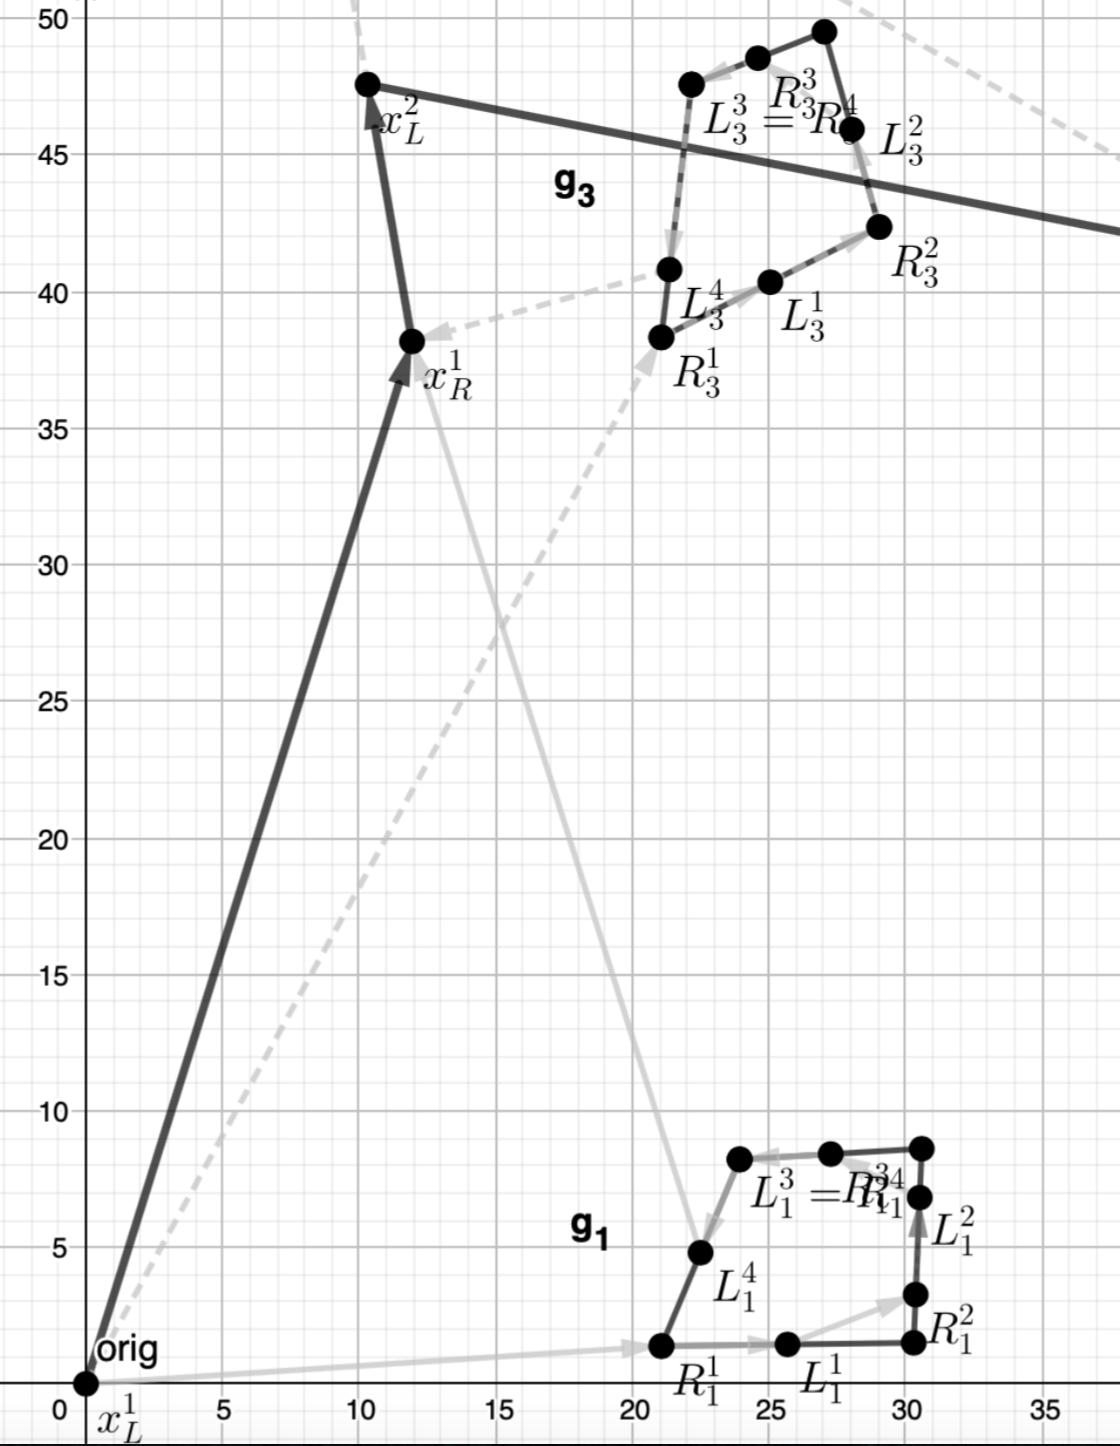
\includegraphics[width=\textwidth]{example_final-g1_g3_gray.png}%
    \caption{}
    \end{subfigure}
	\begin{subfigure}[b]{0.4\textwidth}
	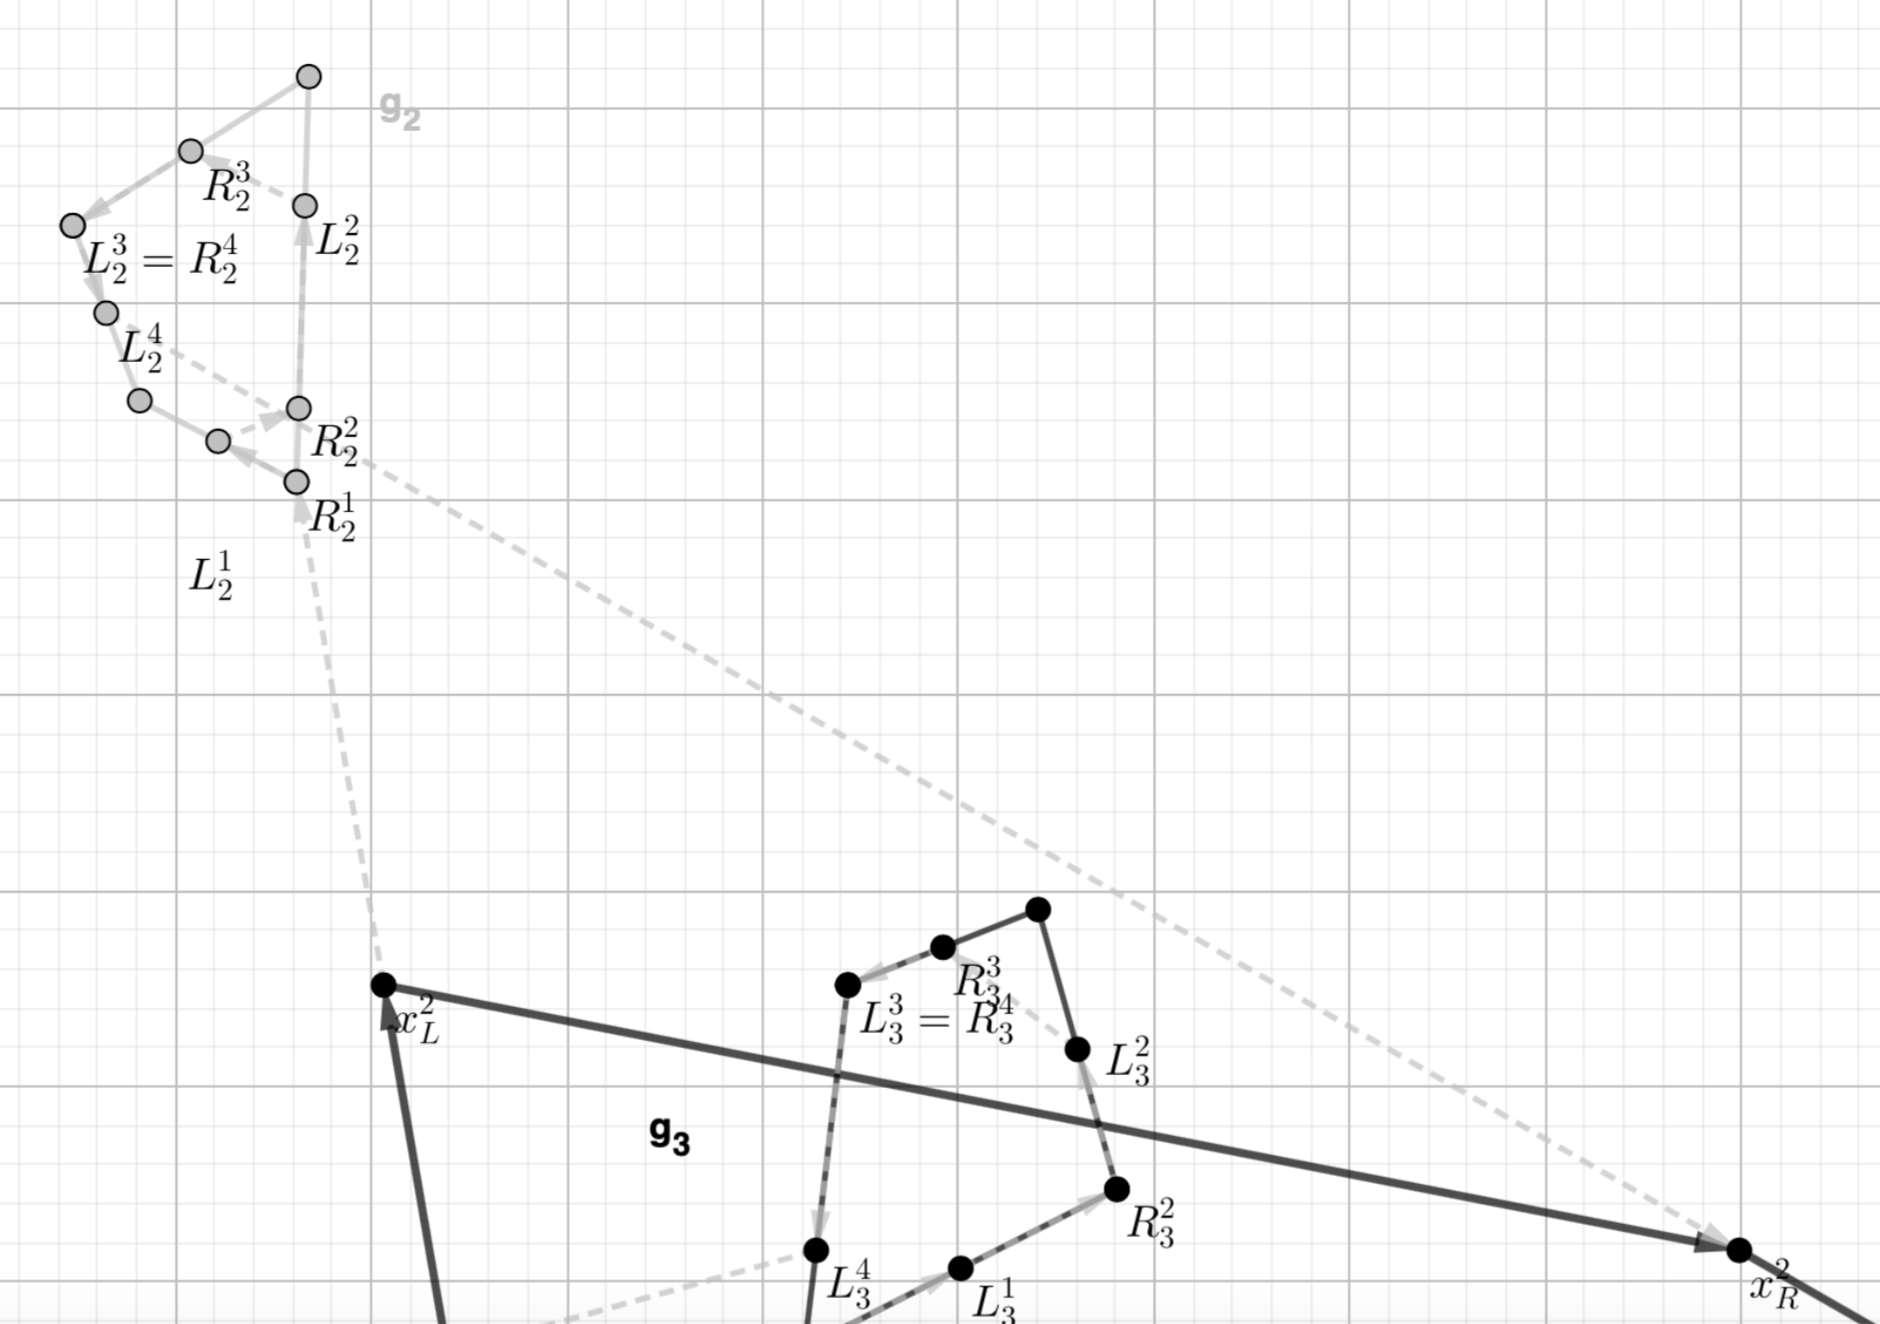
\includegraphics[width=\textwidth]{example_final-g2_gray.png}
	\caption{}%
    \end{subfigure}
	\begin{subfigure}[b]{0.4\textwidth}
	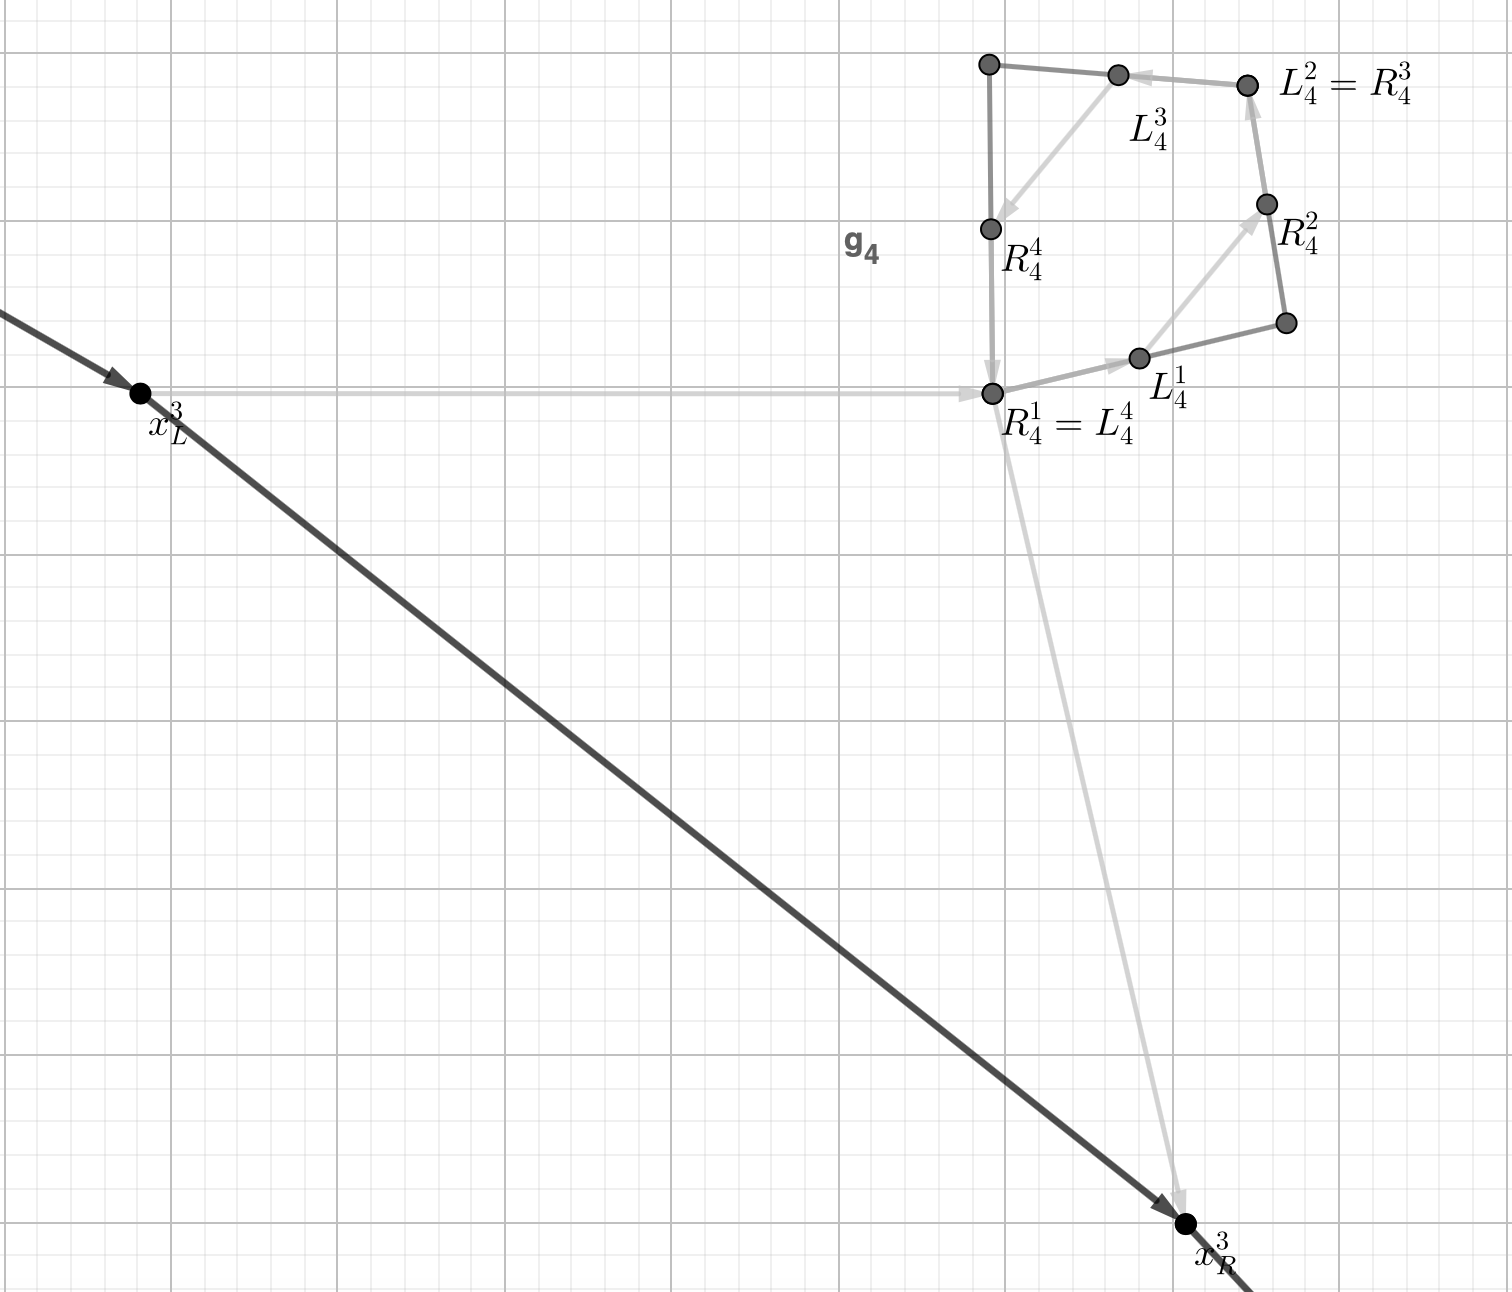
\includegraphics[width=\textwidth]{example_final-g4_gray.png}
	\caption{}
	\end{subfigure}%
    \caption{Zoom on the tour on each target graph provided by STEP 5}%
    \label{fig:example5}%
\end{figure}
%\begin{figure}[h!]
%    \centering
%    \subfloat[\centering a]{{\includegraphics[width=5cm]{example_final-g1_g3.png}}}%
%    \qquad
%    \subfloat[\centering b]{{\includegraphics[width=5cm]{example_final-g2.png} }}%
%     \qquad
%    \subfloat[\centering c]{{\includegraphics[width=5cm]{example_final-g4.png} }}%
%    \caption{Zoom on the tour on each target graph provided by STEP 5}%
%    \label{fig:example5}%
%\end{figure}

\noindent 
Focusing on each single target graph, Figure \ref{fig:example5} shows the zoom on the tours followed by the drones. For example, Figure \ref{fig:example5}[a] reports the one performed by the drone that visits \RE{the} graph $g_1$ \RE{(in pink) and the drone that visits the graph $g_3$ (in sky blue)}. \RE{Both drones start from the mothership at point $x^1_L$ that is the $origin$. One drone first visits the segment $\overline{R^1_1L^1_1}$ of the graph $g_1$, while the other one starts the visit of the graph $g_3$ by traversing the segment $\overline{R^3_1L^3_1}$. From point $L^1_1$ the first drone moves to the second visited edge of the graph $g_1$ by traversing the segment $\overline{R^2_1L^2_1}$. Then, it moves to the third visited edge of graph $g_1$, by flying over the segment $\overline{R^3_1L^3_1}$. From point $R^4_1$ the drone starts the visit of the last edge of graph $g_1$ up to point $L^4_1$. 
Finally, the drone leaves the graph $g_1$ at this latter point and it is retrieved by the mothership at the point $x^1_R$. Similarly, the second drone, that visits the graph $g_3$, after traversing the segment $\overline{R^1_3L^1_3}$, moves to the second visited edge of the same graph and traverses the segment $\overline{R^2_3L^2_3}$. Then, it flies to the third visited edge, by traversing the segment $\overline{R^3_3L^3_3}$. Finally it moves to the last visited edge of the graph $g_3$, by flying over the segment $\overline{R^4_3L^4_3}$. The drone leaves the graph $g_3$ at point $L^4_3$ and reaches the mothership at point $x_R^1$.} 
Note that in this example the drones do not visit the full 100\% of each \RE{graph edge}, but only the half of each one of them.

\bigskip
\noindent
The reader may notice that the above algorithm can be also used to generate solutions for the \RE{partial overlapping model presented in Section \ref{amdasyn} since any solution of the \AMDCO\xspace model is also feasible for the \AMDPO\xspace one as shown in \JP{Theorem \ref{th:relaxation}.}}

\begin{comment}
\JP{ \textbf{\noindent ***   NOT CLEAR THAT WE SHOULD INCLUDE THIS PART  (JUSTO: dixit) ***}
\bigskip

\noindent
As we already explained in Section \ref{amdasyn}, we also studied a variant of the \AMD\space model in which the mothership can launch and retrieve a drone in different stages. We \CV{also} designed a matheuristic (also) for this case with similar steps to the one previously presented.
The idea of this procedure is first solving the model with only one available drone (see \cite{art:Amorosi2021}) to determine the optimal launching/rendezvous points associated with each target graph and the corresponding minimum length of the mothership tour.
Then, a clustering procedure, like the one adopted in the matheuristic proposed for the synchronous case, is performed.
After that, the \AMD\space model without synchronization is solved (on) \CV{for} each cluster\CV{,} setting the launching point of the first cluster equal to the origin. Then the last retrieving point (so) \CV{determined} is set as \CV{the} launching point of the next cluster\CV{,} and so on. From the solution obtained for each cluster\CV{,} the total length of the mothership tour is computed as the sum of the partial lengths of each tour associated with each cluster. The same procedure is repeated by starting the clustering procedure with different random seed.\\
In the following, we present the (pseudo-code) \CV{pseudocode} of this algorithm:

\begin{itemize} 
\item[STEP 1] (Launching/rendezvous points)
Solve the AMDRPG model and let $x_L^g$ and $x_R^g \forall g \in \mathcal{G}$ the associated optimal launching/rendezvous points and let $L$ be the associated minimum length of the mothership tour.  
\item[STEP 2] (Clustering procedure)
Initialization: define one cluster for each target graph and set $nit=1$ \\
Select randomly two clusters $C_i$ and $C_j$ (where $i<j$).\\
Check if the number of graphs belonging to the union of $C_i$ and $C_j$ is less than or equal to the number of available drones $n_D$.\\
If this condition is satisfied:\\
search for the point $C$ satisfying the following \RE{\sout{endurance} endurance} constraint:
$$
\frac{[d(C, R^{e_g}) + C^{e_{g}e^{'}_{g}} + d(C,L^{e^{'}_{g}})]}{v_D} \leq cap \:\: \forall R^{e_g}, L^{e^{'}_{g}} \in C_i, \:\: C_j
$$
If such a point exists, merge the two clusters and assign to the resulting cluster so obtained the label $C_i$.\\

\item[STEP 3](Launch/rendezvous point exchanges)
Set $i=1$ and $x_L=origin$\\
For each cluster $C_i$ generated at STEP 2:\\
- solve the \AMD\space model with first launching point equal to $x_L$.\\
- let $x_R$ be the last rendezvous point associated with the cluster under analysis, set $x_L = x_R$.\\
Let $L'$ be the associated minimum length of the mothership tour computed as sum of the partial lengths of the tours associated with the clusters.\\
If $L' < L$ update the solution.\\
Set $nit=nit+1$.\\
Repeat STEP 2 and STEP 3 while $nit < maxit$
\end{itemize}
}
\end{comment}

% \input{Benders-like}
% \newpage
\section{Experimental results}


% \begin{figure}[h!]
% \begin{center}
%  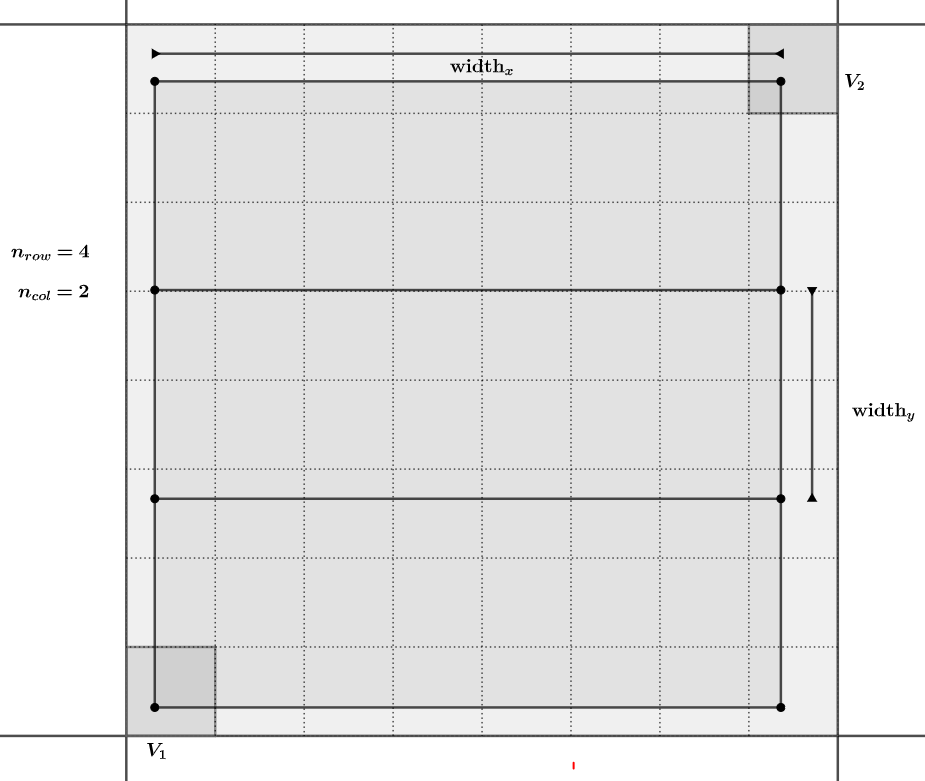
\includegraphics[width=1\linewidth]{Grid_generation.png}
% \end{center}
% \end{figure}
\noindent
In this section we discuss the experimental results obtained testing the formulations presented in Section \ref{Form} and the matheuristic procedure proposed in Section \ref{Math} on a testbed of instances. In particular, we consider instances like the ones used in \cite{art:Amorosi2021} where the targets, to be visited by the drones, are represented by grid graphs.
This set consists of 5 instances of respectively 5 and 10 target graphs, with different cardinality of the set of nodes. More precisely, each instance is composed of 20$\%$ graphs with 4 nodes, 20$\%$ graphs of 6 nodes, 20$\%$ graphs of 8 nodes and 20$\%$ graphs of 10 nodes. Moreover, we assume that the velocity of the drones is twice that of the mothership and that a random percentage of each target graph, or of each of its edges, must be visited by the fleet of drones.\\
We consider in our experiments that the number of drones varies between 1 and 3 and that the drones
endurance (expressed as maximum time that the drone can operate when it is fully recharged) ranges between 20 and 60.
Table \ref{table:tab1} reports a summary of the characteristics of our instances.

\renewcommand{\arraystretch}{0.7}
\begin{table}[!h]
\caption{Instances parameter values}
\centering
\footnotesize
\begin{tabular}{l | c }
\hline
\# Targets & (5,10)\\
\hline
\# Drones &	(1,2,3)\\
\hline
\# Vertices & (4,6,8,10,12)\\
\hline
Drone endurance & (20,30,40,50,60)\\
\hline
$\%$ target (edge) & random variable
\end{tabular}
\label{table:tab1}
\end{table}

\noindent
Table \ref{table:tab2} reports the results obtained solving the \AMD model on the instances previously described, by adopting the commercial solver Gurobi. We consider the exact solution both providing and not providing an initial solution computed by the matheuristic described in Section \ref{Math}. More precisely, the first column of Table \ref{table:tab2} indicates the number of target graphs to be visited by the fleet of drones, the second column reports the endurance of the drones, the third column distinguishes between the visit of a percentage of each edge (e) and the percentage of each target graph (g). The fourth column reports the size of the fleet of drones. Thus, for each combination of the listed parameters, we summarize the average percentage gap of the solution obtained within the time limit set equal to 2 hours. We report respectively average percentage gap with initialization by the solution provided by the matheuristic, solution time, in seconds, of the matheuristic and average gap without initialization by the solution obtained by the matheuristic.\\
We can observe that the value of the average percentage gap ranges between a minimum of 66.9\% and a maximum of 97.43\%. This shows that the model is hard to be solved even on small size instances. Moreover, we can see that in most of the cases, the average percentage gap associated with the variant of the model consisting in visiting a given percentage of each edge, is higher than the one associated with the variant imposing to visit a given percentage of each target graph. Another thing that we can observe is that the average percentage gap increases with the number of drones and decreases with the drone endurance.\\
As regards the number of target graphs, we can see that by increasing it from 5 to 10, the exact method, without initialization by the solution obtained with the matheursitic, becomes even harder. Indeed, the red entries of the table mean that some instances could not find a feasible solution within the time limit (note that in the brackets we indicate the number of these instances). The number of not solvable instances increases with the number of drones. Moreover, for the minimum level of endurance, the exact solution of the model without initialization provided by the matheuristic, does not provide any solution, within the time limit, for instances with 10 graphs and 2 or 3 drones.\\
Considering the comparison with the exact method starting from the solution provided by the matheuristic, we can note that the values of average percentage gap are very close to the ones related to the exact solution method without initialization. Thus the initialization does not speed up the convergence of the solver. However, we can see that the matheuristic is always able to find a feasible solution of the problem, even for the cases in which the solver is not.\\
Moreover, the average solution times of the matheuristic range between a minimum of 37 seconds to a maximum of 3 minutes. They increase with the drone endurance for the variant of the model in which a given percentage of each edge must be visited, while they decrease by increasing the number of drones for the variant of the model in which a given percentage of each target graph must visited. By increasing the number of target graphs from 5 to 10, the average solution times of the matheuristics become more than double for both model variants.
Summing up, the results obtained show that the exact solution method given by solving the formulation is very challenging even for small size instances. However, exploiting it, the matheuristic is able to provide  solutions for all instances rather quickly.


%\begin{table}[!h]
%\caption{Comparison between exact solution with and without initialization by the matheuristic solution}
%\centering
%\tiny
%\begin{tabular}{|c|c|c|c c c c c c c c c|}
%\hline
%\multirow{3}{*}{$\bm{|\mathcal{G}|}$} & \multirow{3}{*}{$\bm{N^d}$}  & \multirow{3}{*}{\textbf{v.t.}} & \multicolumn{9}{|c|}{\textbf{$\#$ drones}} \\
%\cline{4-12}
%& & & \multicolumn{3}{c|}{1} & \multicolumn{3}{c|}{2} & \multicolumn{3}{c|}{3}\\
%\cline{4-12}
%& & &  $\%$Gap (i) & TimeH & $\%$Gap (wi) & $\%$Gap (i) & TimeH & $\%$Gap (wi)& $\%$Gap (i) & TimeH & $\%$Gap (wi)\\
%\hline
%\multirow{5}{*}{\midrule 5} & \multirow{2}{*}{20} & e & 82,63 & 61,56 & 81,70 & 91,57 &	63,80 &	90,61 &	93,06 &	60,87 &	90,93\\
%&  & g & 79,09 & 44,97 & 79,63 & 89,03 & 37,32 & 91,85 & 94,00 & 39,05 & 95,80\\
%\cline{2-12}
%& \multirow{2}{*}{30} & e & 82,70 &	65,21 &	80,17 &	85,14 &	64,41 &	82,21 &	91,90 &	63,34 &	90,12\\
%& & g & 75,80 &	55,77 &	71,19 &	84,36 &	44,36 &	88,27 &	91,02 &	44,59 &	91,39\\
%\cline{2-12}
%& \multirow{2}{*}{40} & e & 80,94 &	68,81 &	77,98 &	83,44 &	64,80 &	82,16 &	91,24 &	63,19 &	86,25\\
%& & g & 74,47 &	43,92 &	73,46 &	81,21 &	38,27 &	84,35 &	85,34 &	37,51 &	89,63\\
%\cline{2-12}
%& \multirow{2}{*}{50} & e & 76,87 &	66,67 &	74,41 &	81,12 &	63,86 &	79,57 &	85,11 &	63,51 &	86,16\\
%& & g & 70,58 &	43,42 &	66,90 &	80,96 &	43,98 &	88,84 &	80,49 &	44,35 &	82,81\\
%\cline{2-12}
%& \multirow{2}{*}{60} & e & 76,39 &	67,78 &	71,61 &	81,63 &	66,08 &	79,84 &	83,82 &	64,40 &	82,06\\
%& & g & 78,17 &	44,69 &	72,79 &	79,35 &	40,63 &	86,55 &	81,74 &	50,01 &	84,66\\
%\hline
%\multirow{5}{*}{10} & \multirow{2}{*}{20} & e & 82,56 &	137,93 &	84,91 &	92,30 &	128,53 & - & 94,73 & 124,44 & -\\
%&  & g & 81,00 & 119,20 & \textcolor{red}{84,08 (2)} & 89,88 & 83,50 & \textcolor{red}{96,64 (2)} & 96,44 & 70,00 & \textcolor{red}{97,43 (3)}\\
%\cline{2-12}
%& \multirow{2}{*}{30} & e & 80,60 &	159,00 & 80,93 & 87,11 & 132,15 & \textcolor{red}{87,58 (3)} &	94,56 &	127,35 & \textcolor{red}{92,85 (2)}\\
%& & g & 79,93 &	132,67 & \textcolor{red}{82,70 (1)} & 86,32 & 80,29 & \textcolor{red}{86,13 (3)} & 91,12 &	76,72 &	\textcolor{red}{89,74 (1)}\\
%\cline{2-12}
%& \multirow{2}{*}{40} & e & 79,05 &	191,37 & 78,07 & 85,11 & 131,26 &	84,33 &	91,88 &	132,10 & \textcolor{red}{88,61 (1)}\\
%& & g & 80,23 &	115,00 & 79,64 & 87,31 & 68,39 & \textcolor{red}{84,57 (3)} & 96,09 &	69,40 &	\textcolor{red}{91,86 (1)}\\
%\cline{2-12}
%& \multirow{2}{*}{50} & e & 81,49 &	188,32 & 77,81 & 87,72 & 134,01 &	\textcolor{red}{85,51 (1)} &	92,68 &	132,82 & \textcolor{red}{90,79 (3)}\\
%& & g & 79,92 &	87,23 &	80,38 &	82,80 &	66,14 &	\textcolor{red}{84,00 (3)} &	92,48 &	64,94 &	\textcolor{red}{91,96 (2)}\\
%\cline{2-12}
%& \multirow{2}{*}{60} & e & 83,79 &	155,27 & 81,57 & 85,91 & 131,94 &	\textcolor{red}{82,96 (2)} &	92,24 &	130,11 & \textcolor{red}{86,58 (3)}\\
%& & g & 77,57 &	97,89 &	78,46 &	86,94 &	76,53 &	\textcolor{red}{88,29 (2)} &	94,31 &	69,53 &	\textcolor{red}{92,23 (3)}\\
%\hline
%\end{tabular}
%\label{table:tab2}
%\end{table}
% Please add the following required packages to your document preamble:
% \usepackage{multirow}
% \usepackage{graphicx}
% \usepackage[table,xcdraw]{xcolor}
% If you use beamer only pass "xcolor=table" option, i.e. \documentclass[xcolor=table]{beamer}
\begin{table}[h!]
\centering
\caption{Comparison between exact solution with and without initialization by the matheuristic solution}
\label{table:tab2}
\resizebox{\textwidth}{!}{%
\begin{tabular}{|c|c|c|ccc|ccc|ccc|}
\hline
 &  &  & \multicolumn{9}{c|}{\textbf{\# drones}} \\ \cline{4-12} 
 &  &  & \multicolumn{3}{c|}{1} & \multicolumn{3}{c|}{2} & \multicolumn{3}{c|}{3} \\ \cline{4-12} 
\multirow{-3}{*}{$\bm{|\mathcal G|}$} & \multirow{-3}{*}{$\bm{N^d}$} & \multirow{-3}{*}{\textbf{v.t.}} & \% Gap (i) & TimeH & \% Gap (wi) & \% Gap (i) & TimeH & \% Gap (wi) & \% Gap (i) & TimeH & \% Gap (wi) \\ \hline
 &  & e & 82,63 & 61,56 & 81,70 & 91,57 & 63,80 & 90,61 & 93,06 & 60,87 & 90,93 \\ \cline{3-3}
 & \multirow{-2}{*}{20} & g & 79,09 & 44,97 & 79,63 & {\color[HTML]{333333} 89,03} & 37,32 & 91,85 & 94,00 & 39,05 & 95,80 \\ \cline{2-12} 
 &  & e & 82,70 & 65,21 & 80,17 & 85,14 & 64,41 & 82,21 & 91,9 & 63,34 & 90,12 \\ \cline{3-3}
 & \multirow{-2}{*}{30} & g & 75,80 & 55,77 & 71,19 & 84,36 & 44,36 & 88,27 & 91,02 & 44,59 & 91,39 \\ \cline{2-12} 
 &  & e & 80,94 & 68,81 & 77,98 & 83,44 & 64,80 & 82,16 & 91,24 & 63,19 & 86,25 \\ \cline{3-3}
 & \multirow{-2}{*}{40} & g & 74,47 & 43,92 & 73,46 & 81,21 & 38,27 & 84,35 & 85,34 & 37,51 & 89,63 \\ \cline{2-12} 
 &  & e & 76,87 & 66,67 & 74,41 & 81,12 & 63,86 & 79,57 & 85,11 & 63,51 & 86,16 \\ \cline{3-3}
 & \multirow{-2}{*}{50} & g & 70,58 & 43,42 & 66,90 & 80,96 & 43,98 & 88,84 & 80,49 & 44,35 & 82,81 \\ \cline{2-12} 
 &  & e & 76,39 & 67,78 & 71,61 & 81,63 & 66,08 & 79,84 & 83,82 & 64,40 & 82,06 \\ \cline{3-3}
\multirow{-10}{*}{5} & \multirow{-2}{*}{60} & g & 78,17 & 44,69 & 72,79 & 79,35 & 40,63 & 86,55 & 81,74 & 50,01 & 84,66 \\ \hline
 &  & e & 82,56 & 137,93 & 84,91 & 92,30 & 128,53 & - & 94,73 & 124,44 & - \\ \cline{3-3}
 & \multirow{-2}{*}{20} & g & 81,00 & 119,20 & {\color[HTML]{FE0000} 84,08 (2)} & 89,88 & 83,50 & {\color[HTML]{FE0000} 96,64 (2)} & 96,44 & 70,00 & {\color[HTML]{FE0000} 97,43 (3)} \\ \cline{2-12} 
 &  & e & 80,60 & 159,00 & 80,93 & 87,11 & 132,15 & {\color[HTML]{FE0000} 87,58 (3)} & 94,56 & 127,35 & {\color[HTML]{FE0000} 92,85 (2)} \\ \cline{3-3}
 & \multirow{-2}{*}{30} & g & 79,93 & 132,67 & {\color[HTML]{FE0000} 82,70 (1)} & 86,32 & 80,29 & {\color[HTML]{FE0000} 86,13 (3)} & 91,12 & 76,72 & {\color[HTML]{FE0000} 89,74 (1)} \\ \cline{2-12} 
 &  & e & 79,05 & 191,37 & 78,07 & 85,11 & 131,26 & 84,33 & 91,88 & 132,10 & {\color[HTML]{FE0000} 88,61 (1)} \\ \cline{3-3}
 & \multirow{-2}{*}{40} & g & 80,23 & 115,00 & 79,64 & 87,31 & 68,39 & {\color[HTML]{FE0000} 84,57 (3)} & 96,09 & 69,40 & {\color[HTML]{FE0000} 91,86 (1)} \\ \cline{2-12} 
 &  & e & 81,49 & 188,32 & 77,81 & 87,72 & 134,01 & {\color[HTML]{FE0000} 85,51 (1)} & 92,68 & 132,82 & {\color[HTML]{FE0000} 90,79 (3)} \\ \cline{3-3}
 & \multirow{-2}{*}{50} & g & 79,92 & 87,23 & 80,38 & 82,80 & 66,14 & {\color[HTML]{FE0000} 84,00 (3)} & 92,48 & 64,94 & {\color[HTML]{FE0000} 91,96 (2)} \\ \cline{2-12} 
 &  & e & 83,79 & 155,27 & 81,57 & 85,91 & 131,94 & {\color[HTML]{FE0000} 82,96 (2)} & 92,24 & 130,11 & {\color[HTML]{FE0000} 86,58 (3)} \\ \cline{3-3}
\multirow{-10}{*}{10} & \multirow{-2}{*}{60} & g & 77,57 & 97,89 & 78,46 & 86,94 & 76,53 & {\color[HTML]{FE0000} 88,29 (2)} & 94,31 & 69,53 & {\color[HTML]{FE0000} 92,23 (3)} \\ \hline
\end{tabular}%
}
\end{table}

\noindent
We show in Figure \ref{fig:heatmap} the relationship between the objective function values of the problem and the number of available drones and their endurance. This figure reports the average objective values of all the instances with three target graphs varying the number of drones in $\{1,2,3\}$ and their endurance (endurance) in $\{10,20,30,40,50,60\}$. The darker the color intensity the smaller the objective value. As expected, our experiment confirms that both, a greater number of drones and larger endurance reduce total length of the mothership route.

\begin{figure}[h!]
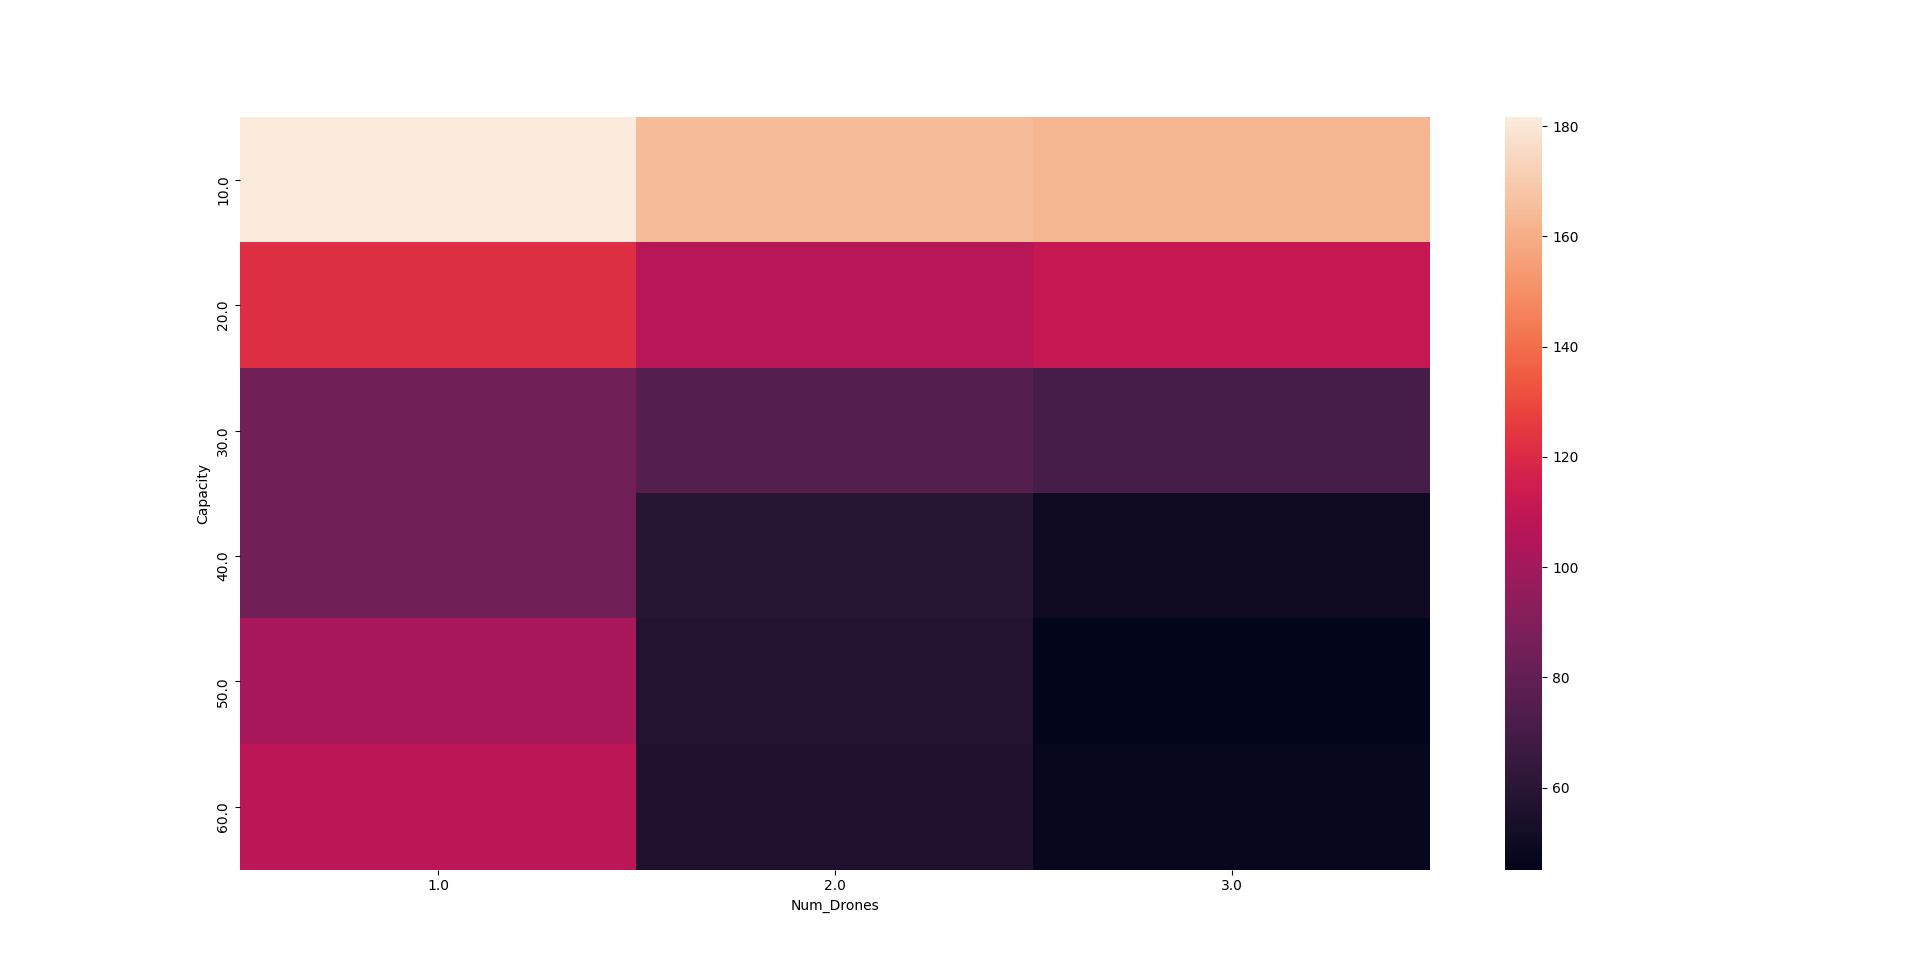
\includegraphics[width=\linewidth]{heatmap.png}
\caption{Heatmap of objective function values depending on number of drones and drone capacities. The darker the color intensity the smaller the objective value. \label{fig:heatmap}}
\end{figure}
\noindent
%In order to test the performances of the matheuristic proposed in Section \ref{Math}, we coded it in Python and we run it on the same sets of instances (Grid and Delaunay) on which the three formulations have been solved. Table \ref{table:tab3} reports for each instance, numbered from 0 to 4, distinguishing between Grid and Delauney, respectively, the best objective function provided by the best formulation, the objective function provided by the matheuristic and the associated CPU time. As already noticed from Table \ref{table:tab2}, for grid graph instances, SEC formulation has the best behaviour, with the exception of the instance number 3 for which the MTZ provides a smaller value of the objective function. As for the Delaunay graph instances, MTZ is the best formulation, but also in this case there is an exception on the instance number 2 for which SEC formulation returns a smaller value of the objective function.\\
%The results show that the matheuristic returns a solution with value of the objective function that is higher than the one provided by the SEC formulation on grid instances. However, these values are smaller than the ones provided by the Stages and the MTZ formulations. Moreover, the saving in terms of resolution time is very significant as the maximum CPU time is less than 1 minute.  As regards the Delaunay instances, the matheuristic performances are even better, as it finds a solution that is better than the best one provided by the MTZ formulation and in a resolution time that is at most 28 minutes. 



%\renewcommand{\arraystretch}{0.7}
%\begin{table}[!h]
%\caption{Heuristic performances}
%\centering
%\footnotesize
%\begin{tabular}{c | c c c | c c c}
%\hline
%\textbf{\#}  & \multicolumn{3}{c}{\textbf{Grid}} &  \multicolumn{3}{c}{\textbf{Delauney}} \\
 % \hline
% &Best Obj & Obj Heuristic &CPU Time &Best Obj & Obj Heuristic & CPU Time \\
%\hline
%0 &	1087,87	& 1117,83 &	50,99 &	947,01 &	934,46 &	52,49\\
%1 &	1100,38	& 1319,64 &	24,64 &	986,22 &	 938,68	& 72,73\\
%2 &	1350,67	& 1126,35 &	46,06 &	888,48 &	865,66 &	1073,80\\
%3 &	1218,66	& 1476,36 &	27,18 &	1249,69 &	1154,62 &	1703,33\\
%4 &	1297,77	& 1424,37 &	40,91 &	1239,93	 & 1184,67 &	81,15\\
%    \hline
%\end{tabular}
%\label{table:tab3}
%\end{table}


\noindent
%We performed a second set of experiments by observing that, even if there are small differences between the SEC and the MTZ formulations depending on the type of instances, their performances are comparable.
%Thus, in the rest of the tests we focused on the MTZ formulation. We compared its performances, with or without providing the initial solution found by the matheuristic, on a set of larger instances. More precisely, we generated 20 instances with targets represented by grid graphs and 20 instances with targets represented by Delauney graphs. The instances of each typology are split in 4 groups of 5 instances each, consisting respectively of 5, 10, 15 and 20 targets to be visited.
%In each instance the same percentage of graphs ($20\%$) has respectively 4, 6, 8, 10 and 12 nodes. 
%Moreover, we assumed that the origin coincides with the destination in all instances and we randomly generated with uniform distribution between 0 and 1, two values representing the percentage of each edge and of each graph to be visited.
%As regards the speeds, we set the speed of the drone three times the one of the mothership.
%We run the MTZ formulation by adopting Gurobi, setting a time limit of 7200 sec. for each instance.
%On the same instances also the matheuristic has been applied. Note that, in order to define a stopping rule for the exact resolution of the AMDRPG model within the matheuristic procedure (STEP 3 and STEP 4), we set the maximum number of solutions generated by the solver equal to five.
%For each instance, the solution provided by the matheuristic has been then used to initialize the exact resolution of the MTZ formulation in order to try to speed up the resolution process.
%Table \ref{table:tab4} shows the results of the comparison between the exact resolution of the formulation with and without initialization. In the first column, named List, we report the size of the instances in terms of number of targets to be visited (0, 1, 2 and 3 identifies instances respectively with 5, 10, 15 and 20 graphs).The second column refers to the two variants of the model, that is, a given percentage of each edge of the targets (e) or a given percentage of each target (g) must be visited by the drone. The other columns report respectively the average percentage gap of the solutions found within the time limit starting from the initial solution provided by the matheuristic, the average running time of the matheuristic and the average percentage gap of the solutions found within the time limit without initialization. These information are reported for both Grid and Delauney instances.

%\renewcommand{\arraystretch}{0.7}
%\begin{table}[!h]
%\caption{Comparison between exact resolution with and without initialization}
%\centering
%\footnotesize
%\begin{tabular}{c c | c c c | c c c}
%\hline
% &  & \multicolumn{3}{c}{\textbf{Grid}} &  \multicolumn{3}{c}{\textbf{Delauney}} \\
%\hline
% List &  $\%$  & $\%$ Gap (i) & Time$\_$h & $\%$ Gap (ni)  & $\%$ Gap (i) & Time$\_$h &  $\%$ Gap (ni)\\
%\hline
%\multirow{}{}{0} & e & 0.72 & 105.12 & 0.73 & 0.78 & 154.92 & 0.74\\
%& g & 0.55 & 58.92 & 0.54 & 0.62 & 92.64 & 0.67\\
%\hline
%\multirow{}{}{1} & e & 0.76 & 241.99 & 0.76 & 0.80 & 314.69 & 0.79\\
%& g & 0.71 & 182.61 & 0.70 & 0.74 & 353.04 & 0.75\\
%\hline
%\multirow{}{}{2} & e & 0.76 & 367.69 & 0.76 & 0.80 & 447.61 & 0.80 \\
%& g & 0.71 & 326.49 & 0.72 & 0.76 & 429.16 & 0.76\\
%\hline
%\multirow{}{}{3} & e & 0.75 & 481.68 & 0.74 & 0.80 & 514.98 & 0.76^*\\
%& g & 0.71 & 492.27 & 0.70 & 0.77 & 582.90 & 0.77\\
%    \hline
%\end{tabular}
%\label{table:tab4}
%\end{table}

\noindent
%From Table \ref{table:tab4} we can notice that in most of the cases the average gaps associated with the solution found within the time limit, with and without initialization by the solution found by the matheuristic, are the same or very close (note that in the last column the $*$ indicates that only one instance has been solved within the time limit).
%As regards the running time of the matheuristic, we can see also from the boxplots in Figure \ref{fig:1}, that it increases with the number of targets to be visited both for Grid and Delaunay instances. Considering the model variants based on the minimum percentage of each edge or each graph to visit, we can observe that for Grid instances the average running time of the model imposing a minimum percentage of each edge to be visited, is greater than the one associated with the other variant, with the exception of the instances of biggest size (List=3). \\
\noindent
%The boxplots in Figure \ref{fig:2} represent the percentage gap of the solution provided by the matheuristic with respect to the one provided by the exact resolution of the MTZ model within the time limit, with initialization by the solution found by the matheuristic. From them we can notice that the gap increases with the size both for Grid and Delaunay instances but it is always less than 0.5$\%$.  
%Figure \ref{fig:3} shows the percentage gap of the solution provided by the exact resolution of the MTZ formulation within the time limit without the initialization, with respect to the one found with the initialization. This gap is very close to 0 both for Grid and Delaunay instances. Only for the biggest size we observe values ranging between 0.1$\%$ and 0.6$\%$. These observations suggest that, even if the initialization of the model by the solution provided by the matheuristic does not speed up the convergence to the optimal solution, the matheuristic provides solutions of very good quality. Indeed, it generates in less than 10 minutes solutions that are very close to the ones provided by the model within 2 hours.\\


%\begin{figure}[htp]% [H] is so declass\'e!
%\centering
%\begin{minipage}{0.45\textwidth}
%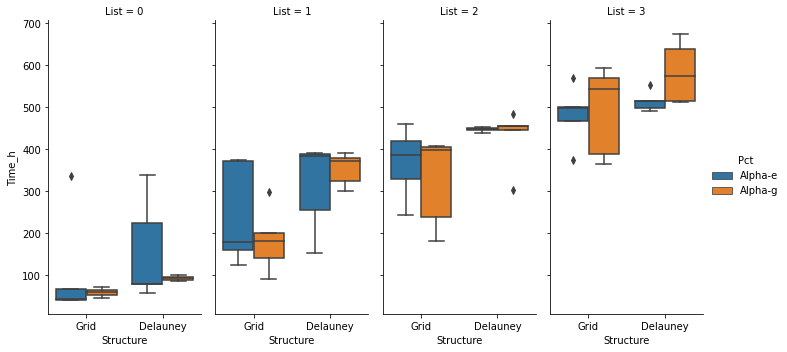
\includegraphics[width=\textwidth]{time_h.png}
%\caption{Matheuristic running time}
%\label{fig:1}
%\end{minipage}\hfill
%\begin{minipage}{0.45\textwidth}
%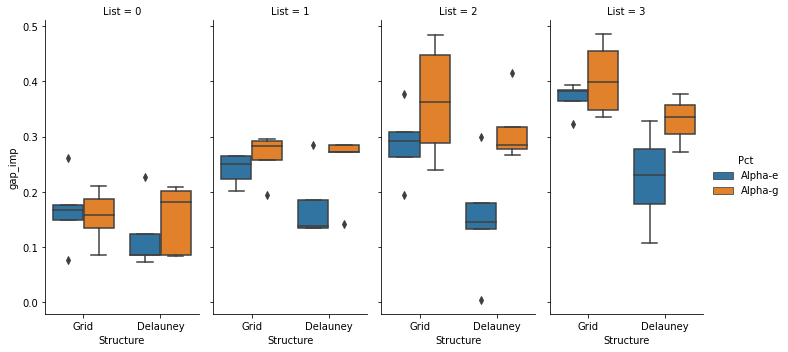
\includegraphics[width=\textwidth]{improved_gap.png}
%\caption{Matheuristic improved gap}
%\label{fig:2}
%\end{minipage}\par
%\vskip\floatsep% normal separation between figures
%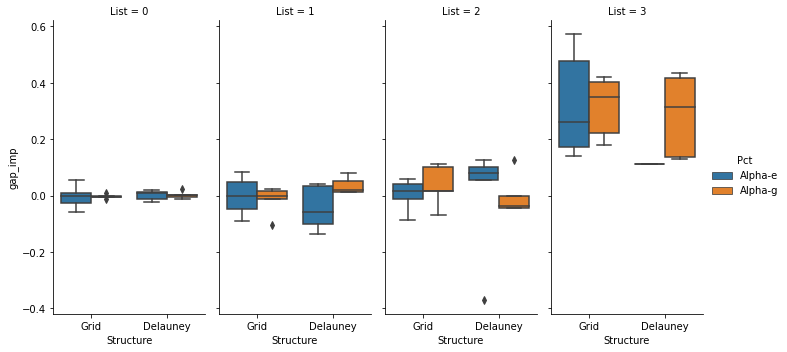
\includegraphics[width=0.45\textwidth]{differencewithwithout.png}
%\caption{Improved gap of MTZ formulation with and without initialization}
%\label{fig:3}
%\end{figure}



%\noindent
%As regards the \NMD \xspace problem, we generated three sets of instances with targets represented by grid graphs considering different structures of the polygonal network where the mothership can move.
%In particular, we defined a first set of instances where the mothership network is represented by a graph of 6 nodes with a tree structure with origin of the path of the base vehicle different from the destination.
%A second set of instances involving a mothership network consisting in a complete graph of 4 vertices with origin of the path of the base vehicle different from the destination.  
%A third set of instances characterized by star graphs of 7 nodes representing the mothership network, where the origin coincides with the destination and it is located at the centre of the star. We generated 10 instances for each of these three classes, 5 of them with 5 targets and 5 with 10 targets to be visited. 
%Moreover, as for the AMDRPG, for each of these 10 instances we randomly generated two values representing the percentage of each edge and of each graph that must be visited by the drone.
%We run on these sets of instances both Stages and MTZ formulations. Table \ref{table:tab5} summarizes the results obtained comparing them. The first column identifies the size of the instances, similarly to Table \ref{table:tab4}, (0 for instances with 5 targets and 1 for instances with 10 targets).
%The second column distinguishes between minimum percentage of each edge (e) or of each graph (g) to be visited by the drone.
%The remaining columns refer to the three different class  of instances described above (1 for the networks with a tree structure, 2 for complete networks and 3 for start networks).
%For each of these sets of instances the average percentage gap of the solutions found within the time limit of 7200 sec. by the two formulations (Stages and MTZ) is reported.


%\renewcommand{\arraystretch}{0.7}
%\begin{table}[!h]
%\caption{Comparison between formulations of \NMD}
%\centering
%\footnotesize
%\begin{tabular}{c c | c c | c c | c c}
%\hline
% & Net Struct  & \multicolumn{2}{c}{1} &  \multicolumn{2}{c}{2}  & \multicolumn{2}{c}{3}\\
%\hline
%List & $\%$ &  Stages  & MTZ & Stages & MTZ  & Stages & MTZ\\
%\hline
%\multirow{}{}{0} & e & 0.89 & 0.33 & 0.88 & 0.24 & 0.87 & 0.39\\
%& g & 0.86 & 0.29 & 0.89 & 0.18 & 0.90 & 0.42\\
%\hline
%\multirow{}{}{1} & e & 0.92 & 0.43 & 0.92 & 0.33 & 0.92 & 0.46\\
%& g & 0.91 & 0.36 & 0.92 & 0.23 & 0.92 & 0.39\\
%\hline
%\end{tabular}
%\label{table:tab5}
%\end{table}

\noindent
%We can observe that for each class of instances and model variants, based on the percentage of each edge or each graph to be visited, the MTZ formulation performs better than the Stages one. In all the cases the percentage average gap associated with the MTZ formulation is one third or half of that associated with the Stages formulation. For this reason, in the following tests, related to the comparison between the exact resolution of the \NMD\xspace  model with and without the initialization by the solution found by the matheuristic, we focused only on the MTZ formulation.\\
%Table \ref{table:tab6} summarizes the results of this comparison distinguishing again between the different network structures (columns labelled 1, 2 and 3), the different size (rows labelled 0 and 1) characterizing the instances and model variants (minimum percentage of each edge (e) or each graph (g) to be visited). For each combination of network structure, size and model variant we reported the average percentage gap with initialization ($\%$ Gap (i)), the solution time of the matheuristic (T$\_$h) and the average percentage gap without initialization by the solution found by the matheuristic ($\%$ Gap (ni))

%\renewcommand{\arraystretch}{0.8}
%\begin{table}[!h]
%\caption{Comparison between exact resolution with and without initialization of \NMD}
%\centering
%\scriptsize
%\begin{tabular}{c c | c c c | c c c | c c c}
%\hline
% & Net Struct  & \multicolumn{3}{c}{1} &  \multicolumn{3}{c}{2}  & \multicolumn{3}{c}{3}\\
%\hline
%List &  $\%$  & $\%$ Gap (i) & T$\_$h & $\%$ Gap (ni)  & $\%$ Gap (i) & T$\_$h &  $\%$ Gap (ni) & $\%$ Gap (i) & T$\_$h &  $\%$ Gap (ni)\\
%\hline
%\multirow{}{}{0} & e & 0.32 & 109.96 & 0.33 & 0.24 & 207 & 0.24 & 0.39 & 177.57 & 0.39\\
%& g & 0.30 & 110.92 & 0.29 & 0.18 & 163.36 & 0.18 & 0.45 & 149.68 & 0.42\\
%\hline
%\multirow{}{}{1} & e & 0.48 & 1030.64 & 0.43 & 0.39 & 802.3 & 0.33 & 0.53 & 770.05 & 0.46\\
%& g & 0.33 & 479.36 & 0.36 & 0.35 & 639.09 & 0.23 & 0.42 & 689.51 & 0.39\\
%\hline
%\end{tabular}
%\label{table:tab6}
%\end{table}

\noindent
%We can observe that, similarly to the AMDRPG problem, the average gaps associated with the solution found within the time limit, with and without initialization by the solution found by the matheuristic, are very close. Considering the average running time we can notice that the \NMD\xspace  problem is more challanging to be solved with respect to the AMDRPG. It increases very fast with the size of the instances especially for the case in which the network where the mothership moves has a tree structure. Moreover, as for the Grid instances in the continuous case, the model variant imposing a minimum percentage of each edge to be visited takes more time to be solved.

%\begin{figure}
%\centering
%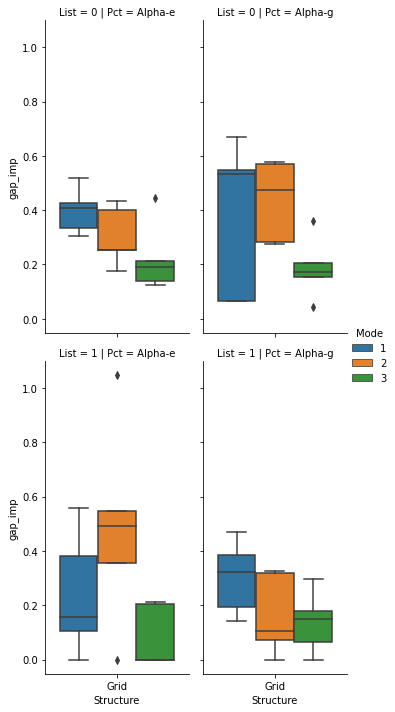
\includegraphics[width=5cm]{improved_gap_ND.png}
%\caption{Matheuristic improved gap for \NMD}
%\label{fig:4}
%\end{figure}
\noindent
%The boxplots showed in Figure \ref{fig:4} report the percentage gap of the solution provided by the matheuristic with respect to the one provided by the exact resolution of the MTZ model within the time limit, with initialization by the solution found by the matheuristic.
%We can notice that, excluding the outliers, this gap ranges between 0$\%$ and 0.7$\%$ and its lowest values are observed for the instances in which the network where the mothership moves has a star structure (green boxplots). 
%From the previous observations, similarly to the AMDRPG, we can conclude that the behaviour of the matheuristic is very good in terms of quality of the solutions provided, even if the initialization of the MTZ model does not help in speeding up the convergence to the optimal solution. 












\section{Experimental results\label{section:results}}


% \begin{figure}[h!]
% \begin{center}
%  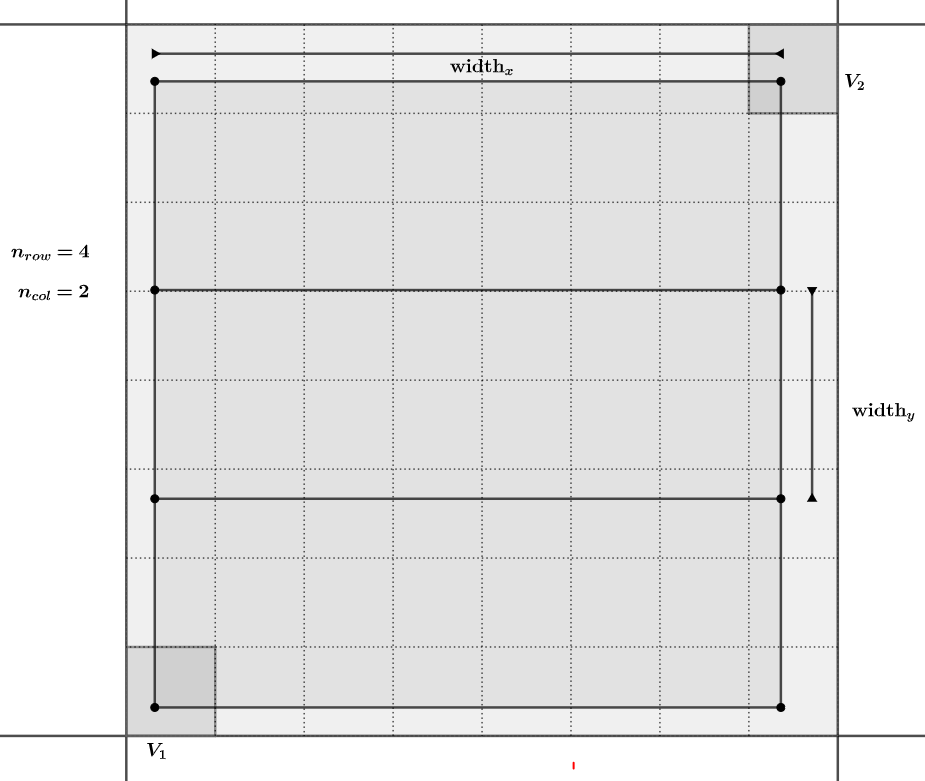
\includegraphics[width=1\linewidth]{Grid_generation.png}
% \end{center}
% \end{figure}
\noindent
In this section\RE{,} we discuss the experimental results obtained testing the formulations presented in Section \ref{Form} and the matheuristic procedure proposed in Section \ref{Math} on a testbed of instances. In particular, we consider instances like the ones used in \cite{art:Amorosi2021}\RE{,} where the targets to be visited by the drones are represented by grid graphs.
\RE{We have generated one set of 5 instances with 5 graphs and \RE{another} set of 5 instances with 10 graphs.} More precisely, each instance is composed of 20$\%$ graphs with 4 nodes, 20$\%$ graphs of 6 nodes, 20$\%$ graphs of 8 nodes, 20$\%$ graphs of 10 nodes and \RE{and 20$\%$ graphs with 12 nodes}. Moreover, we assume that the velocity of the drones is twice that of the mothership and that a random \RE{fraction} of each target graph, or of each of its edges, must be visited by the fleet of drones. \RE{These fractions are uniform randomly sampled in the interval $(0, 1)$.}\\

\noindent
%\subsection{\CV{ADD TITLE TO THE FIRST EXPERIMENT}} 
We consider in our experiments that the number of drones varies between 1 and 3 and that the drone endurance (expressed as \RE{the} maximum time that the drone can operate when it is fully recharged) ranges between 20 and 60. \RE{Note that the case of a single drone is also included in our experiments to compare the results and complexity of using one and more than one drones. \RE{The interested reader is referred to \cite{art:Amorosi2021} for analyzing} the complexity in terms of gap of the model with a single drone.}
Table \ref{table:tab1} reports a summary of the characteristics of our instances.

\renewcommand{\arraystretch}{0.7}
\begin{table}[!h]
\caption{Instances parameter values}
\centering
\footnotesize
\begin{tabular}{c | c }
\hline
\RE{$|\mathcal G|$} & (5,10)\\
\hline
\RE{$|\mathcal D|$} &	(1,2,3)\\
\hline
\RE{$|V_g|$} & (4,6,8,10,12)\\
\hline
\RE{$N_D$} & (20,30,40,50,60)\\
\hline
\RE{fraction} target (edge) & \RE{uniform randomly sampled in $(0, 1)$.}
\end{tabular}
\label{table:tab1}
\end{table}

\noindent
We coded the matheuristic and the exact resolution of the model in Python 3.8.10. The mathematical programming formulation has been implemented in Gurobi 9.1.2. All the tests have been run on a machine AMD® Epyc 7402p with 24-core processor × 8.
Table \ref{table:tab2} reports the results obtained solving \LA{both variants} of the \AMD\xspace model on the instances previously described, by adopting the commercial solver Gurobi. We consider the exact solution both providing and not providing an initial solution computed by the matheuristic described in Section \ref{Math}. More precisely, the first \LA{row} of Table \ref{table:tab2} indicates \LA{the model variant and the second row reports the number of target graphs to be visited by the fleet of drones (5 or 10). From the third row, we split each column in three sub-columns. The first three sub-columns report respectively, the endurance of the drones, the size of the fleet of drones and the indication on the visit of a \RE{fraction} of each edge (e) or a \RE{fraction} of each target graph (g). From sub-column 4 to sub-column 15, we report, for each combination of the listed parameters characterizing the instances, respectively, the average gap without initialization by the solution provided by the matheuristic (wi), the average gap with initialization by the solution obtained by the matheuristic (i) and the solution time, in seconds, of the matheuristic (TimeH). The time limit of these experiments is set equal to 1 hour.}\\
\noindent
\LA{We can observe that the value of the average percentage gap ranges between a minimum of 58\% and a maximum of 100\%. This shows that the model is hard to be solved even with small size instances. Moreover, we can see that for the complete overlapping version of the model, in most of the cases, the average gap associated with the variant of the model consisting in visiting a given \RE{fraction} of each edge, is higher than the one associated with the variant imposing to visit a given \RE{fraction} of each target graph. 
%The opposite behaviour can be observed for the partial overlapping version of the model.
Another thing that we can observe is that the average percentage gap increases with the number of target graphs for both problem variants.\\
\noindent
Moreover, the reader may note that the partial overlapping version of the problem is harder to solve than the complete overlapping version by looking at the values of the average gap. This is an expected behaviour due to the fact that the feasible region of the partial overlapping variant contains the one associated with the complete overlapping variant, as proven in Theorem \ref{th:relaxation}. 
We can see that for both versions of the problem, by increasing the number of target graphs from 5 to 10, the exact method without initialization \RE{of} the solution obtained with the \RE{matheuristic}, becomes even harder. Indeed, the red entries of the table mean that some instances could not find a feasible solution within the time limit (note that in the brackets we indicate the number of these instances).} %The number of not \RE{solved} instances increases with the number of drones.
\LA{In addition, for the minimum level of endurance, the exact solution of the partial overlapping model without initialization provided by the matheuristic, does not find any solution within the time limit for instances with 10 graphs, 3 drones and a given fraction of each edge to be visited. The same can be observed also for the exact solution of the complete overlapping model without initialization provided by the matheuristic, for a level of endurance equal to 30, a fleet of 3 drones and a given fraction of each edge to be visited.}\\
Considering the comparison with the exact method starting from the solution provided by the matheuristic, we can note that the values of the average percentage gap are very close to the ones related to the exact solution method without initialization. Thus\RE{,} the initialization does not speed up the convergence of the solver. However, we can see that the matheuristic is always able to find a feasible solution of the problem, even for the cases in which the solver is not. 

%\RE{INCLUDE EXPLANATION OF THE BOXPLOTS}
\noindent
\LA{Furthermore, the average solution times of the matheuristic range between a minimum of 4 seconds to a maximum of 9.5 minutes. In particular, we can observe that, in most of the cases, for the complete overlapping version of the problem, the matheuristic running time is shorter for the instances where a fraction of the length of each graph is required to be visited. The same behaviour can be noticed for the partial overlapping version of the problem for which the difference in terms of running time is even bigger. Indeed, when a given fraction of the length of each edge is required, STEP 1 of the matheuristic (computation of the TSP over the graph edges) takes more time.} %They increase with the drone \RE{endurance} for the variant of the model in which a given \RE{fraction} of each edge must be visited, while they decrease by increasing the number of drones for the variant of the model in which a given \RE{fraction} of each target graph must \RE{be} visited. 
\LA{By increasing the number of target graphs from 5 to 10, the average solution times of the matheuristic increases for both model variants.}
Summing up, the results obtained show that the exact solution method given by solving the formulation is very challenging even for small size instances. However, exploiting it, the matheuristic is able to provide  solutions for all instances rather quickly.
% Please add the following required packages to your document preamble:
% Table generated by Excel2LaTeX from sheet 'Hoja2'
\begin{table}[h!]
  \centering
  \caption{\JP{Comparison between the partial and complete overlapping models}}
    \resizebox{\textwidth}{!}{
    \begin{tabular}{|c|c|c||ccc|ccc||ccc|ccc|}
    \hline
    \multicolumn{3}{|c|}{\textbf{Model}} & \multicolumn{6}{c|}{Complete Overlapping}     & \multicolumn{6}{c|}{Partial Overlapping} \bigstrut\\
    \hline
    \multicolumn{3}{|c|}{$|\mathcal G|$} & \multicolumn{3}{c|}{5} & \multicolumn{3}{c|}{10} & \multicolumn{3}{c|}{5} & \multicolumn{3}{c|}{10} \bigstrut\\
    \hline
    $N_D$ & $|\mathcal D|$ & $\alpha$ & Gap (wi) & Gap (i) & TimeH & Gap (wi) & Gap (i) & TimeH & Gap (wi) & Gap (i) & TimeH & Gap (wi) & Gap (i) & TimeH \bigstrut\\
    \hline
    \hline
    \multirow{6}[6]{*}{20} & \multirow{2}[2]{*}{1} & g     & 0,78  & 0,79  & 6,01  & \textcolor[rgb]{ 1,  0,  0}{0,91 (2)} & 0,86  & 177,69 & 0,65  & 0,63  & 16,53 & 1     & 1     & 215,59 \bigstrut[t]\\
          &       & e     & 0,81  & 0,81  & 15,41 & \textcolor[rgb]{ 1,  0,  0}{0,89 (2)} & 0,84  & 148,95 & 0,84  & 0,83  & 52,36 & \textcolor[rgb]{ 1,  0,  0}{0,88 (3)} & 0,87  & 440,93 \bigstrut[b]\\
\cline{2-15}          & \multirow{2}[2]{*}{2} & g     & 0,81  & 0,87  & 5,76  & \textcolor[rgb]{ 1,  0,  0}{0,96 (3)} & 0,96  & 139,24 & 0,97  & 0,96  & 13,91 & \textcolor[rgb]{ 1,  0,  0}{1 (3)} & 1     & 76,77 \bigstrut[t]\\
          &       & e     & 0,93  & 0,92  & 33,99 & \textcolor[rgb]{ 1,  0,  0}{0,97 (3)} & 0,97  & 163,41 & \textcolor[rgb]{ 1,  0,  0}{0,86 (2)} & 0,85  & 66,38 & \textcolor[rgb]{ 1,  0,  0}{0,89 (4)} & 0,85  & 578,31 \bigstrut[b]\\
\cline{2-15}          & \multirow{2}[2]{*}{3} & g     & 0,88  & 0,89  & 4,83  & \textcolor[rgb]{ 1,  0,  0}{0,95 (3)} & 0,94  & 67,76 & 0,97  & 0,97  & 17,87 & \textcolor[rgb]{ 1,  0,  0}{1 (2)} & 1     & 18,88 \bigstrut[t]\\
          &       & e     & 0,92  & 0,91  & 14,08 & \textcolor[rgb]{ 1,  0,  0}{0,97 (2)} & 0,97  & 125,89 & \textcolor[rgb]{ 1,  0,  0}{0,81 (3)} & 0,84  & 61,83 & \textcolor[rgb]{ 1,  0,  0}{- (5)} & 0,82  & 237,33 \bigstrut[b]\\
    \hline
    \hline
    \multirow{6}[6]{*}{30} & \multirow{2}[2]{*}{1} & g     & 0,71  & 0,7   & 9,66  & \textcolor[rgb]{ 1,  0,  0}{0,82 (4)} & 0,82  & 87,4  & 0,77  & 0,75  & 15,43 & 1     & 1     & 39,83 \bigstrut[t]\\
          &       & e     & 0,79  & 0,8   & 14,16 & \textcolor[rgb]{ 1,  0,  0}{0,8 (4)} & 0,83  & 122,23 & 0,84  & 0,82  & 38,94 & \textcolor[rgb]{ 1,  0,  0}{0,83 (4)} & 0,81  & 289,74 \bigstrut[b]\\
\cline{2-15}          & \multirow{2}[2]{*}{2} & g     & 0,82  & 0,82  & 4,98  & \textcolor[rgb]{ 1,  0,  0}{0,95 (3)} & 0,92  & 174,64 & 0,97  & 0,96  & 12,94 & 1     & 1     & 45,37 \bigstrut[t]\\
          &       & e     & 0,84  & 0,84  & 14,73 & \textcolor[rgb]{ 1,  0,  0}{0,96 (3)} & 0,97  & 133,75 & 0,78  & 0,79  & 31,82 & 0,82  & 0,77  & 171,16 \bigstrut[b]\\
\cline{2-15}          & \multirow{2}[2]{*}{3} & g     & 0,82  & 0,81  & 4,63  & \textcolor[rgb]{ 1,  0,  0}{0,93 (3)} & 0,95  & 105,54 & 0,96  & 0,96  & 16,22 & 1     & 1     & 33,95 \bigstrut[t]\\
          &       & e     & 0,88  & 0,89  & 12,08 & \textcolor[rgb]{ 1,  0,  0}{- (5)} & 0,97  & 127,78 & 0,83  & 0,82  & 35,38 & \textcolor[rgb]{ 1,  0,  0}{0,79 (3)} & 0,8   & 213,06 \bigstrut[b]\\
    \hline
    \hline
    \multirow{6}[6]{*}{40} & \multirow{2}[2]{*}{1} & g     & 0,68  & 0,68  & 5,79  & \textcolor[rgb]{ 1,  0,  0}{0,81 (2)} & 0,82  & 93,21 & 0,73  & 0,71  & 11,46 & 1     & 1     & 48,85 \bigstrut[t]\\
          &       & e     & 0,76  & 0,77  & 37,55 & \textcolor[rgb]{ 1,  0,  0}{0,78 (4)} & 0,81  & 160,24 & 0,8   & 0,79  & 57,28 & \textcolor[rgb]{ 1,  0,  0}{0,79 (1)} & 0,8   & 403,72 \bigstrut[b]\\
\cline{2-15}          & \multirow{2}[2]{*}{2} & g     & 0,72  & 0,66  & 5,14  & \textcolor[rgb]{ 1,  0,  0}{0,91 (2)} & 0,92  & 131,26 & 0,96  & 0,95  & 11,48 & 1     & 1     & 35,71 \bigstrut[t]\\
          &       & e     & 0,83  & 0,78  & 19,46 & \textcolor[rgb]{ 1,  0,  0}{0,91 (2)} & 0,95  & 141,6 & 0,79  & 0,79  & 35,79 & \textcolor[rgb]{ 1,  0,  0}{0,79 (1)} & 0,79  & 576,75 \bigstrut[b]\\
\cline{2-15}          & \multirow{2}[2]{*}{3} & g     & 0,61  & 0,62  & 3,91  & 0,91  & 0,91  & 115,48 & 0,95  & 0,95  & 15,13 & 1     & 1     & 17,98 \bigstrut[t]\\
          &       & e     & 0,85  & 0,83  & 15,36 & 0,93  & 0,94  & 85,9  & 0,81  & 0,81  & 40,37 & \textcolor[rgb]{ 1,  0,  0}{0,81 (1)} & 0,8   & 309,09 \bigstrut[b]\\
    \hline
    \hline
    \multirow{6}[6]{*}{50} & \multirow{2}[2]{*}{1} & g     & 0,65  & 0,64  & 5,52  & \textcolor[rgb]{ 1,  0,  0}{0,82 (3)} & 0,84  & 101,24 & 0,82  & 0,78  & 9,53  & 1     & 1     & 32,54 \bigstrut[t]\\
          &       & e     & 0,74  & 0,73  & 16,63 & \textcolor[rgb]{ 1,  0,  0}{0,81 (3)} & 0,83  & 118,67 & 0,78  & 0,77  & 58,95 & \textcolor[rgb]{ 1,  0,  0}{0,82 (2)} & 0,82  & 311,02 \bigstrut[b]\\
\cline{2-15}          & \multirow{2}[2]{*}{2} & g     & 0,7   & 0,7   & 6,37  & \textcolor[rgb]{ 1,  0,  0}{0,9 (1)} & 0,93  & 206,87 & 0,97  & 0,97  & 14,68 & 1     & 1     & 39,5 \bigstrut[t]\\
          &       & e     & 0,67  & 0,73  & 12,07 & \textcolor[rgb]{ 1,  0,  0}{0,92 (2)} & 0,93  & 168,57 & 0,77  & 0,77  & 36,46 & \textcolor[rgb]{ 1,  0,  0}{0,8 (1)} & 0,81  & 265,16 \bigstrut[b]\\
\cline{2-15}          & \multirow{2}[2]{*}{3} & g     & 0,65  & 0,64  & 4,27  & \textcolor[rgb]{ 1,  0,  0}{0,9 (1)} & 0,93  & 26,68 & 0,94  & 0,92  & 19,08 & 1     & 1     & 15,97 \bigstrut[t]\\
          &       & e     & 0,74  & 0,74  & 12,95 & 0,9   & 0,94  & 90,14 & 0,8   & 0,79  & 40,77 & \textcolor[rgb]{ 1,  0,  0}{0,76 (3)} & 0,79  & 195,68 \bigstrut[b]\\
    \hline
    \hline
    \multirow{6}[6]{*}{60} & \multirow{2}[2]{*}{1} & g     & 0,69  & 0,7   & 5,58  & \textcolor[rgb]{ 1,  0,  0}{0,8 (4)} & 0,81  & 83,02 & 0,78  & 0,76  & 11,18 & 1     & 1     & 36,78 \bigstrut[t]\\
          &       & e     & 0,74  & 0,74  & 16,53 & \textcolor[rgb]{ 1,  0,  0}{0,85 (2)} & 0,86  & 145,06 & 0,76  & 0,76  & 37,73 & \textcolor[rgb]{ 1,  0,  0}{0,84 (2)} & 0,83  & 359,68 \bigstrut[b]\\
\cline{2-15}          & \multirow{2}[2]{*}{2} & g     & 0,67  & 0,72  & 4,09  & \textcolor[rgb]{ 1,  0,  0}{0,94 (2)} & 0,94  & 81,69 & 0,95  & 0,94  & 13,33 & 1     & 1     & 17,04 \bigstrut[t]\\
          &       & e     & 0,76  & 0,73  & 15,58 & \textcolor[rgb]{ 1,  0,  0}{0,94 (2)} & 0,92  & 108,17 & 0,78  & 0,78  & 33,28 & 0,78  & 0,79  & 237,38 \bigstrut[b]\\
\cline{2-15}          & \multirow{2}[2]{*}{3} & g     & 0,58  & 0,53  & 7     & \textcolor[rgb]{ 1,  0,  0}{0,89 (2)} & 0,9   & 60,99 & 0,91  & 0,94  & 20,15 & 1     & 1     & 33,93 \bigstrut[t]\\
          &       & e     & 0,72  & 0,7   & 15,39 & \textcolor[rgb]{ 1,  0,  0}{0,91 (2)} & 0,96  & 96,52 & 0,78  & 0,78  & 49,39 & 0,81  & 0,81  & 259,34 \bigstrut[b]\\
    \hline
    \end{tabular}}%
  \label{table:tab2}%
\end{table}%

\noindent
\LA{The boxplots in Figure \ref{fig:gap_boxplot_synchronous}  represent the relative gap of the solution provided by the matheuristic for the complete overlapping version of the problem, with respect to the one provided by the exact solution of the \RE{mathematical programming} model within the time limit, with the initialization of the solution found by the matheuristic. Similarly, Figure \ref{fig:gap_boxplot_asynchronous} reports the same information for the partial overlapping version of the problem.}

% % This file was created with tikzplotlib v0.9.12.
\definecolor{color0}{rgb}{0.917647058823529,0.917647058823529,0.949019607843137}
\definecolor{color1}{rgb}{0.347058823529412,0.458823529411765,0.641176470588235}
\definecolor{color2}{rgb}{0.798529411764706,0.536764705882353,0.389705882352941}

\begin{figure}[h!]
\centering
\begin{tikzpicture}[scale=0.6]

\begin{axis}[
axis background/.style={fill=color0},
axis line style={white},
tick align=outside,
title={$|\mathcal D| = 1$},
x grid style={white},
xtick pos = left,
ytick pos = left,
xlabel={$|\mathcal G|$},
xmin=-0.5, xmax=1.5,
xtick style={color=white!15!black},
xtick={0,1},
xticklabels={5,10},
y grid style={white},
ylabel={Relative Gap},
ymajorgrids,
ymin=-2.0023571013993, ymax=54.6854669223967,
ytick style={color=white!15!black}
]
\path [draw=white!29.8039215686275!black, fill=color1, semithick]
(axis cs:-0.396,21.7888049191559)
--(axis cs:-0.004,21.7888049191559)
--(axis cs:-0.004,30.8406843661928)
--(axis cs:-0.396,30.8406843661928)
--(axis cs:-0.396,21.7888049191559)
--cycle;
\path [draw=white!29.8039215686275!black, fill=color2, semithick]
(axis cs:0.004,18.4793987935756)
--(axis cs:0.396,18.4793987935756)
--(axis cs:0.396,27.9849884101838)
--(axis cs:0.004,27.9849884101838)
--(axis cs:0.004,18.4793987935756)
--cycle;
\path [draw=white!29.8039215686275!black, fill=color1, semithick]
(axis cs:0.604,0.00874895880390045)
--(axis cs:0.996,0.00874895880390045)
--(axis cs:0.996,4.51419914610234)
--(axis cs:0.604,4.51419914610234)
--(axis cs:0.604,0.00874895880390045)
--cycle;
\path [draw=white!29.8039215686275!black, fill=color2, semithick]
(axis cs:1.004,0.0020834572568334)
--(axis cs:1.396,0.0020834572568334)
--(axis cs:1.396,0.0669377251793516)
--(axis cs:1.004,0.0669377251793516)
--(axis cs:1.004,0.0020834572568334)
--cycle;
\draw[draw=white!29.8039215686275!black,fill=color1,line width=0.3pt] (axis cs:0,0) rectangle (axis cs:0,0);
\draw[draw=white!29.8039215686275!black,fill=color1,line width=0.3pt] (axis cs:0,0) rectangle (axis cs:0,0);
\addlegendimage{ybar,ybar legend,draw=white!29.8039215686275!black,fill=color1,line width=0.3pt}
\addlegendentry{\% graph}

\draw[draw=white!29.8039215686275!black,fill=color2,line width=0.3pt] (axis cs:0,0) rectangle (axis cs:0,0);
\addlegendimage{ybar,ybar legend,draw=white!29.8039215686275!black,fill=color2,line width=0.3pt}
\addlegendentry{\% edge}

\addplot [semithick, white!29.8039215686275!black]
table {%
-0.2 21.7888049191559
-0.2 9.87718961543874
};
\addplot [semithick, white!29.8039215686275!black]
table {%
-0.2 30.8406843661928
-0.2 40.828071376835
};
\addplot [semithick, white!29.8039215686275!black]
table {%
-0.298 9.87718961543874
-0.102 9.87718961543874
};
\addplot [semithick, white!29.8039215686275!black]
table {%
-0.298 40.828071376835
-0.102 40.828071376835
};
\addplot [black, mark=diamond*, mark size=2.5, mark options={solid,fill=white!29.8039215686275!black}, only marks]
table {%
-0.2 45.5638022037681
};
\addplot [semithick, white!29.8039215686275!black]
table {%
0.2 18.4793987935756
0.2 7.03956951402302
};
\addplot [semithick, white!29.8039215686275!black]
table {%
0.2 27.9849884101838
0.2 35.4418303987987
};
\addplot [semithick, white!29.8039215686275!black]
table {%
0.102 7.03956951402302
0.298 7.03956951402302
};
\addplot [semithick, white!29.8039215686275!black]
table {%
0.102 35.4418303987987
0.298 35.4418303987987
};
\addplot [black, mark=diamond*, mark size=2.5, mark options={solid,fill=white!29.8039215686275!black}, only marks]
table {%
0.2 3.42933486135715
};
\addplot [semithick, white!29.8039215686275!black]
table {%
0.8 0.00874895880390045
0.8 0
};
\addplot [semithick, white!29.8039215686275!black]
table {%
0.8 4.51419914610234
0.8 10.2651385218831
};
\addplot [semithick, white!29.8039215686275!black]
table {%
0.702 0
0.898 0
};
\addplot [semithick, white!29.8039215686275!black]
table {%
0.702 10.2651385218831
0.898 10.2651385218831
};
\addplot [black, mark=diamond*, mark size=2.5, mark options={solid,fill=white!29.8039215686275!black}, only marks]
table {%
0.8 19.9251319119723
};
\addplot [semithick, white!29.8039215686275!black]
table {%
1.2 0.0020834572568334
1.2 -1.3353502544535e-14
};
\addplot [semithick, white!29.8039215686275!black]
table {%
1.2 0.0669377251793516
1.2 0.0939379065004709
};
\addplot [semithick, white!29.8039215686275!black]
table {%
1.102 -1.3353502544535e-14
1.298 -1.3353502544535e-14
};
\addplot [semithick, white!29.8039215686275!black]
table {%
1.102 0.0939379065004709
1.298 0.0939379065004709
};
\addplot [black, mark=diamond*, mark size=2.5, mark options={solid,fill=white!29.8039215686275!black}, only marks]
table {%
1.2 3.30798611427499
1.2 1.65360546285996
1.2 12.4879588505733
};
\addplot [semithick, white!29.8039215686275!black]
table {%
-0.396 26.6321353435948
-0.004 26.6321353435948
};
\addplot [semithick, white!29.8039215686275!black]
table {%
0.004 22.3311968283402
0.396 22.3311968283402
};
\addplot [semithick, white!29.8039215686275!black]
table {%
0.604 0.241511938215122
0.996 0.241511938215122
};
\addplot [semithick, white!29.8039215686275!black]
table {%
1.004 0.0136998158227596
1.396 0.0136998158227596
};
\end{axis}
\end{tikzpicture}
\begin{tikzpicture}[scale = 0.6]
\begin{axis}[
axis background/.style={fill=color0},
axis line style={white},
tick align=outside,
title={$|\mathcal D| = 2$},
x grid style={white},
xtick pos = left,
ytick pos = left,
xlabel={$|\mathcal G|$},
xmin=-0.5, xmax=1.5,
xtick style={color=white!15!black},
xtick={0,1},
xticklabels={5,10},
y grid style={white},
ylabel={Relative Gap},
ymajorgrids,
ymin=-2.0023571013993, ymax=54.6854669223967,
ytick style={color=white!15!black}
]
\path [draw=white!29.8039215686275!black, fill=color1, semithick]
(axis cs:-0.396,24.2908680304667)
--(axis cs:-0.004,24.2908680304667)
--(axis cs:-0.004,38.9734345321689)
--(axis cs:-0.396,38.9734345321689)
--(axis cs:-0.396,24.2908680304667)
--cycle;
\path [draw=white!29.8039215686275!black, fill=color2, semithick]
(axis cs:0.004,13.6199008648404)
--(axis cs:0.396,13.6199008648404)
--(axis cs:0.396,28.8801759071672)
--(axis cs:0.004,28.8801759071672)
--(axis cs:0.004,13.6199008648404)
--cycle;
\path [draw=white!29.8039215686275!black, fill=color1, semithick]
(axis cs:0.604,0.0328401107308227)
--(axis cs:0.996,0.0328401107308227)
--(axis cs:0.996,16.3389014643552)
--(axis cs:0.604,16.3389014643552)
--(axis cs:0.604,0.0328401107308227)
--cycle;
\path [draw=white!29.8039215686275!black, fill=color2, semithick]
(axis cs:1.004,0.018119712131219)
--(axis cs:1.396,0.018119712131219)
--(axis cs:1.396,2.05799457575158)
--(axis cs:1.004,2.05799457575158)
--(axis cs:1.004,0.018119712131219)
--cycle;
\draw[draw=white!29.8039215686275!black,fill=color1,line width=0.3pt] (axis cs:0,0) rectangle (axis cs:0,0);
\addlegendimage{ybar,ybar legend,draw=white!29.8039215686275!black,fill=color1,line width=0.3pt}
\addlegendentry{\% graph}

\draw[draw=white!29.8039215686275!black,fill=color2,line width=0.3pt] (axis cs:0,0) rectangle (axis cs:0,0);
\addlegendimage{ybar,ybar legend,draw=white!29.8039215686275!black,fill=color2,line width=0.3pt}
\addlegendentry{\% edge}
\draw[draw=white!29.8039215686275!black,fill=color1,line width=0.3pt] (axis cs:0,0) rectangle (axis cs:0,0);
\draw[draw=white!29.8039215686275!black,fill=color2,line width=0.3pt] (axis cs:0,0) rectangle (axis cs:0,0);
\addplot [semithick, white!29.8039215686275!black]
table {%
-0.2 24.2908680304667
-0.2 10.4474623283978
};
\addplot [semithick, white!29.8039215686275!black]
table {%
-0.2 38.9734345321689
-0.2 52.0813970689492
};
\addplot [semithick, white!29.8039215686275!black]
table {%
-0.298 10.4474623283978
-0.102 10.4474623283978
};
\addplot [semithick, white!29.8039215686275!black]
table {%
-0.298 52.0813970689492
-0.102 52.0813970689492
};
\addplot [semithick, white!29.8039215686275!black]
table {%
0.2 13.6199008648404
0.2 7.13365300294341e-06
};
\addplot [semithick, white!29.8039215686275!black]
table {%
0.2 28.8801759071672
0.2 38.6874614170675
};
\addplot [semithick, white!29.8039215686275!black]
table {%
0.102 7.13365300294341e-06
0.298 7.13365300294341e-06
};
\addplot [semithick, white!29.8039215686275!black]
table {%
0.102 38.6874614170675
0.298 38.6874614170675
};
\addplot [semithick, white!29.8039215686275!black]
table {%
0.8 0.0328401107308227
0.8 0
};
\addplot [semithick, white!29.8039215686275!black]
table {%
0.8 16.3389014643552
0.8 24.5633566326984
};
\addplot [semithick, white!29.8039215686275!black]
table {%
0.702 0
0.898 0
};
\addplot [semithick, white!29.8039215686275!black]
table {%
0.702 24.5633566326984
0.898 24.5633566326984
};
\addplot [semithick, white!29.8039215686275!black]
table {%
1.2 0.018119712131219
1.2 0
};
\addplot [semithick, white!29.8039215686275!black]
table {%
1.2 2.05799457575158
1.2 2.05799457575158
};
\addplot [semithick, white!29.8039215686275!black]
table {%
1.102 0
1.298 0
};
\addplot [semithick, white!29.8039215686275!black]
table {%
1.102 2.05799457575158
1.298 2.05799457575158
};
\addplot [black, mark=diamond*, mark size=2.5, mark options={solid,fill=white!29.8039215686275!black}, only marks]
table {%
1.2 11.5527375588776
1.2 22.8746077530694
1.2 24.5217334511995
1.2 34.5349113191651
1.2 8.9029594424669
1.2 14.1613847472345
};
\addplot [semithick, white!29.8039215686275!black]
table {%
-0.396 28.4878031388385
-0.004 28.4878031388385
};
\addplot [semithick, white!29.8039215686275!black]
table {%
0.004 21.8875260151041
0.396 21.8875260151041
};
\addplot [semithick, white!29.8039215686275!black]
table {%
0.604 1.99685736233386
0.996 1.99685736233386
};
\addplot [semithick, white!29.8039215686275!black]
table {%
1.004 0.672152105031548
1.396 0.672152105031548
};
\end{axis}
\end{tikzpicture}
\begin{tikzpicture}[scale = 0.6]
\begin{axis}[
axis background/.style={fill=color0},
axis line style={white},
tick align=outside,
title={$|\mathcal D| = 3$},
x grid style={white},
xtick pos = left,
ytick pos = left,
xlabel={$|\mathcal G|$},
xmin=-0.5, xmax=1.5,
xtick style={color=white!15!black},
xtick={0,1},
xticklabels={5,10},
y grid style={white},
ylabel={Relative Gap},
ymajorgrids,
ymin=-2.0023571013993, ymax=54.6854669223967,
ytick style={color=white!15!black}
]
\path [draw=white!29.8039215686275!black, fill=color1, semithick]
(axis cs:-0.396,19.4786101400453)
--(axis cs:-0.004,19.4786101400453)
--(axis cs:-0.004,34.4617472367364)
--(axis cs:-0.396,34.4617472367364)
--(axis cs:-0.396,19.4786101400453)
--cycle;
\path [draw=white!29.8039215686275!black, fill=color2, semithick]
(axis cs:0.004,11.6307680369222)
--(axis cs:0.396,11.6307680369222)
--(axis cs:0.396,27.593386872566)
--(axis cs:0.004,27.593386872566)
--(axis cs:0.004,11.6307680369222)
--cycle;
\path [draw=white!29.8039215686275!black, fill=color1, semithick]
(axis cs:0.604,0.0153042661953022)
--(axis cs:0.996,0.0153042661953022)
--(axis cs:0.996,10.8860101762497)
--(axis cs:0.604,10.8860101762497)
--(axis cs:0.604,0.0153042661953022)
--cycle;
\path [draw=white!29.8039215686275!black, fill=color2, semithick]
(axis cs:1.004,0.0926366637998731)
--(axis cs:1.396,0.0926366637998731)
--(axis cs:1.396,12.6414099793463)
--(axis cs:1.004,12.6414099793463)
--(axis cs:1.004,0.0926366637998731)
--cycle;
\draw[draw=white!29.8039215686275!black,fill=color1,line width=0.3pt] (axis cs:0,0) rectangle (axis cs:0,0);
\addlegendimage{ybar,ybar legend,draw=white!29.8039215686275!black,fill=color1,line width=0.3pt}
\addlegendentry{\% graph}

\draw[draw=white!29.8039215686275!black,fill=color2,line width=0.3pt] (axis cs:0,0) rectangle (axis cs:0,0);
\addlegendimage{ybar,ybar legend,draw=white!29.8039215686275!black,fill=color2,line width=0.3pt}
\addlegendentry{\% edge}
\draw[draw=white!29.8039215686275!black,fill=color1,line width=0.3pt] (axis cs:0,0) rectangle (axis cs:0,0);
\draw[draw=white!29.8039215686275!black,fill=color2,line width=0.3pt] (axis cs:0,0) rectangle (axis cs:0,0);
\addplot [semithick, white!29.8039215686275!black]
table {%
-0.2 19.4786101400453
-0.2 14.3600714974331
};
\addplot [semithick, white!29.8039215686275!black]
table {%
-0.2 34.4617472367364
-0.2 45.5815915247392
};
\addplot [semithick, white!29.8039215686275!black]
table {%
-0.298 14.3600714974331
-0.102 14.3600714974331
};
\addplot [semithick, white!29.8039215686275!black]
table {%
-0.298 45.5815915247392
-0.102 45.5815915247392
};
\addplot [semithick, white!29.8039215686275!black]
table {%
0.2 11.6307680369222
0.2 0
};
\addplot [semithick, white!29.8039215686275!black]
table {%
0.2 27.593386872566
0.2 43.0903230193938
};
\addplot [semithick, white!29.8039215686275!black]
table {%
0.102 0
0.298 0
};
\addplot [semithick, white!29.8039215686275!black]
table {%
0.102 43.0903230193938
0.298 43.0903230193938
};
\addplot [semithick, white!29.8039215686275!black]
table {%
0.8 0.0153042661953022
0.8 0
};
\addplot [semithick, white!29.8039215686275!black]
table {%
0.8 10.8860101762497
0.8 16.4617414417269
};
\addplot [semithick, white!29.8039215686275!black]
table {%
0.702 0
0.898 0
};
\addplot [semithick, white!29.8039215686275!black]
table {%
0.702 16.4617414417269
0.898 16.4617414417269
};
\addplot [semithick, white!29.8039215686275!black]
table {%
1.2 0.0926366637998731
1.2 0
};
\addplot [semithick, white!29.8039215686275!black]
table {%
1.2 12.6414099793463
1.2 27.2419248135531
};
\addplot [semithick, white!29.8039215686275!black]
table {%
1.102 0
1.298 0
};
\addplot [semithick, white!29.8039215686275!black]
table {%
1.102 27.2419248135531
1.298 27.2419248135531
};
\addplot [semithick, white!29.8039215686275!black]
table {%
-0.396 27.5658718997128
-0.004 27.5658718997128
};
\addplot [semithick, white!29.8039215686275!black]
table {%
0.004 21.5787147317098
0.396 21.5787147317098
};
\addplot [semithick, white!29.8039215686275!black]
table {%
0.604 3.74263341643573
0.996 3.74263341643573
};
\addplot [semithick, white!29.8039215686275!black]
table {%
1.004 7.62592534857705
1.396 7.62592534857705
};
\end{axis}
\end{tikzpicture}
\caption{Relative gap boxplots for \AMDCO}
\label{fig:gap_boxplot_synchronous}
\end{figure}
% This file was created with tikzplotlib v0.9.12.
\definecolor{color0}{rgb}{0.9176470,0.9176470,0.94901960}
\definecolor{color1}{rgb}{0.347058,0.4588235,0.6411764}
\definecolor{color2}{rgb}{0.79852941,0.536764,0.3897058}

\begin{figure}[h!]
\centering
\begin{tikzpicture}[scale=0.6]

\begin{axis}[
axis background/.style={fill=color0},
axis line style={white},
tick align=outside,
title={$|\mathcal D|$ = 1},
x grid style={white},
xlabel=\textcolor{white!15!black}{$|\mathcal G|$},
xtick pos = left,
ytick pos = left,
xmin=-0.5, xmax=1.5,
xtick style={color=white!15!black},
xtick={0,1},
xticklabels={5,10},
y grid style={white},
ylabel=\textcolor{white!15!black}{Relative Gap},
ymajorgrids,
ymin=-2.62609180192484, ymax=55.1479278404217,
ytick style={color=white!15!black}
]
\path [draw=white!29.8039215686275!black, fill=color1, semithick]
(axis cs:-0.396,23.351171126429)
--(axis cs:-0.004,23.351171126429)
--(axis cs:-0.004,29.1428581886508)
--(axis cs:-0.396,29.1428581886508)
--(axis cs:-0.396,23.351171126429)
--cycle;
\path [draw=white!29.8039215686275!black, fill=color2, semithick]
(axis cs:0.004,11.7176590067474)
--(axis cs:0.396,11.7176590067474)
--(axis cs:0.396,23.2397374756161)
--(axis cs:0.004,23.2397374756161)
--(axis cs:0.004,11.7176590067474)
--cycle;
\path [draw=white!29.8039215686275!black, fill=color1, semithick]
(axis cs:0.604,0)
--(axis cs:0.996,0)
--(axis cs:0.996,4.91567244371752)
--(axis cs:0.604,4.91567244371752)
--(axis cs:0.604,0)
--cycle;
\path [draw=white!29.8039215686275!black, fill=color2, semithick]
(axis cs:1.004,0)
--(axis cs:1.396,0)
--(axis cs:1.396,0)
--(axis cs:1.004,0)
--(axis cs:1.004,0)
--cycle;
\draw[draw=white!29.8039215686275!black,fill=color1,line width=0.3pt] (axis cs:0,0) rectangle (axis cs:0,0);
\addlegendimage{ybar,ybar legend,draw=white!29.8039215686275!black,fill=color1,line width=0.3pt}
\addlegendentry{\% graph}

\draw[draw=white!29.8039215686275!black,fill=color2,line width=0.3pt] (axis cs:0,0) rectangle (axis cs:0,0);
\addlegendimage{ybar,ybar legend,draw=white!29.8039215686275!black,fill=color2,line width=0.3pt}
\addlegendentry{\% edge}

\addplot [semithick, white!29.8039215686275!black]
table {%
-0.2 23.351171126429
-0.2 20.2948309102868
};
\addplot [semithick, white!29.8039215686275!black]
table {%
-0.2 29.1428581886508
-0.2 37.7174995502607
};
\addplot [semithick, white!29.8039215686275!black]
table {%
-0.298 20.2948309102868
-0.102 20.2948309102868
};
\addplot [semithick, white!29.8039215686275!black]
table {%
-0.298 37.7174995502607
-0.102 37.7174995502607
};
\addplot [black, mark=diamond*, mark size=2.5, mark options={solid,fill=white!29.8039215686275!black}, only marks]
table {%
-0.2 10.7436731274202
-0.2 0.532520584131128
-0.2 11.63870481964
-0.2 38.5383150484397
};
\addplot [semithick, white!29.8039215686275!black]
table {%
0.2 11.7176590067474
0.2 0
};
\addplot [semithick, white!29.8039215686275!black]
table {%
0.2 23.2397374756161
0.2 32.3710612542474
};
\addplot [semithick, white!29.8039215686275!black]
table {%
0.102 0
0.298 0
};
\addplot [semithick, white!29.8039215686275!black]
table {%
0.102 32.3710612542474
0.298 32.3710612542474
};
\addplot [semithick, white!29.8039215686275!black]
table {%
0.8 0
0.8 0
};
\addplot [semithick, white!29.8039215686275!black]
table {%
0.8 4.91567244371752
0.8 8.74627321462437
};
\addplot [semithick, white!29.8039215686275!black]
table {%
0.702 0
0.898 0
};
\addplot [semithick, white!29.8039215686275!black]
table {%
0.702 8.74627321462437
0.898 8.74627321462437
};
\addplot [black, mark=diamond*, mark size=2.5, mark options={solid,fill=white!29.8039215686275!black}, only marks]
table {%
0.8 19.7135319472805
0.8 22.8600948091405
0.8 17.5254820302641
};
\addplot [semithick, white!29.8039215686275!black]
table {%
1.2 0
1.2 0
};
\addplot [semithick, white!29.8039215686275!black]
table {%
1.2 0
1.2 0
};
\addplot [semithick, white!29.8039215686275!black]
table {%
1.102 0
1.298 0
};
\addplot [semithick, white!29.8039215686275!black]
table {%
1.102 0
1.298 0
};
\addplot [black, mark=diamond*, mark size=2.5, mark options={solid,fill=white!29.8039215686275!black}, only marks]
table {%
1.2 5.01285212584406
1.2 12.6187782464826
1.2 3.60850467468294
1.2 5.50654876776942
};
\addplot [semithick, white!29.8039215686275!black]
table {%
-0.396 26.3941988580451
-0.004 26.3941988580451
};
\addplot [semithick, white!29.8039215686275!black]
table {%
0.004 19.8419895666702
0.396 19.8419895666702
};
\addplot [semithick, white!29.8039215686275!black]
table {%
0.604 0
0.996 0
};
\addplot [semithick, white!29.8039215686275!black]
table {%
1.004 0
1.396 0
};
\end{axis}
\end{tikzpicture}
\begin{tikzpicture}[scale = 0.6]
\begin{axis}[
axis background/.style={fill=color0},
axis line style={white},
tick align=outside,
title={$|\mathcal D|$ = 2},
x grid style={white},
xlabel=\textcolor{white!15!black}{$|\mathcal G|$},
xtick pos = left,
ytick pos = left,
xmin=-0.5, xmax=1.5,
xtick style={color=white!15!black},
xtick={0,1},
xticklabels={5,10},
y grid style={white},
ylabel=\textcolor{white!15!black}{Relative Gap},
ymajorgrids,
ymin=-2.62609180192484, ymax=55.1479278404217,
ytick style={color=white!15!black}
]
\path [draw=white!29.8039215686275!black, fill=color1, semithick]
(axis cs:-0.396,19.9290413160217)
--(axis cs:-0.004,19.9290413160217)
--(axis cs:-0.004,34.1534565237393)
--(axis cs:-0.396,34.1534565237393)
--(axis cs:-0.396,19.9290413160217)
--cycle;
\path [draw=white!29.8039215686275!black, fill=color2, semithick]
(axis cs:0.004,13.8445034768791)
--(axis cs:0.396,13.8445034768791)
--(axis cs:0.396,25.9198033064554)
--(axis cs:0.004,25.9198033064554)
--(axis cs:0.004,13.8445034768791)
--cycle;
\path [draw=white!29.8039215686275!black, fill=color1, semithick]
(axis cs:0.604,0)
--(axis cs:0.996,0)
--(axis cs:0.996,9.44492782733373)
--(axis cs:0.604,9.44492782733373)
--(axis cs:0.604,0)
--cycle;
\path [draw=white!29.8039215686275!black, fill=color2, semithick]
(axis cs:1.004,0)
--(axis cs:1.396,0)
--(axis cs:1.396,9.95730680242487)
--(axis cs:1.004,9.95730680242487)
--(axis cs:1.004,0)
--cycle;
\draw[draw=white!29.8039215686275!black,fill=color1,line width=0.3pt] (axis cs:0,0) rectangle (axis cs:0,0);
\addlegendimage{ybar,ybar legend,draw=white!29.8039215686275!black,fill=color1,line width=0.3pt}
\addlegendentry{\% graph}

\draw[draw=white!29.8039215686275!black,fill=color2,line width=0.3pt] (axis cs:0,0) rectangle (axis cs:0,0);
\addlegendimage{ybar,ybar legend,draw=white!29.8039215686275!black,fill=color2,line width=0.3pt}
\addlegendentry{\% edge}
\addplot [semithick, white!29.8039215686275!black]
table {%
-0.2 19.9290413160217
-0.2 8.56923471336534
};
\addplot [semithick, white!29.8039215686275!black]
table {%
-0.2 34.1534565237393
-0.2 41.461981811718
};
\addplot [semithick, white!29.8039215686275!black]
table {%
-0.298 8.56923471336534
-0.102 8.56923471336534
};
\addplot [semithick, white!29.8039215686275!black]
table {%
-0.298 41.461981811718
-0.102 41.461981811718
};
\addplot [semithick, white!29.8039215686275!black]
table {%
0.2 13.8445034768791
0.2 0
};
\addplot [semithick, white!29.8039215686275!black]
table {%
0.2 25.9198033064554
0.2 39.6956477504428
};
\addplot [semithick, white!29.8039215686275!black]
table {%
0.102 0
0.298 0
};
\addplot [semithick, white!29.8039215686275!black]
table {%
0.102 39.6956477504428
0.298 39.6956477504428
};
\addplot [semithick, white!29.8039215686275!black]
table {%
0.8 0
0.8 0
};
\addplot [semithick, white!29.8039215686275!black]
table {%
0.8 9.44492782733373
0.8 20.424957302526
};
\addplot [semithick, white!29.8039215686275!black]
table {%
0.702 0
0.898 0
};
\addplot [semithick, white!29.8039215686275!black]
table {%
0.702 20.424957302526
0.898 20.424957302526
};
\addplot [black, mark=diamond*, mark size=2.5, mark options={solid,fill=white!29.8039215686275!black}, only marks]
table {%
0.8 38.5697950554177
0.8 24.8433139698412
};
\addplot [semithick, white!29.8039215686275!black]
table {%
1.2 0
1.2 0
};
\addplot [semithick, white!29.8039215686275!black]
table {%
1.2 9.95730680242487
1.2 17.5555017835489
};
\addplot [semithick, white!29.8039215686275!black]
table {%
1.102 0
1.298 0
};
\addplot [semithick, white!29.8039215686275!black]
table {%
1.102 17.5555017835489
1.298 17.5555017835489
};
\addplot [black, mark=diamond*, mark size=2.5, mark options={solid,fill=white!29.8039215686275!black}, only marks]
table {%
1.2 31.522609110702
};
\addplot [semithick, white!29.8039215686275!black]
table {%
-0.396 29.4917032318658
-0.004 29.4917032318658
};
\addplot [semithick, white!29.8039215686275!black]
table {%
0.004 16.8115230551657
0.396 16.8115230551657
};
\addplot [semithick, white!29.8039215686275!black]
table {%
0.604 2.90644304969017
0.996 2.90644304969017
};
\addplot [semithick, white!29.8039215686275!black]
table {%
1.004 0
1.396 0
};
\end{axis}
\end{tikzpicture}
\begin{tikzpicture}[scale = 0.6]
\begin{axis}[
axis background/.style={fill=color0},
axis line style={white},
tick align=outside,
title={$|\mathcal D|$ = 3},
x grid style={white},
xlabel=\textcolor{white!15!black}{$|\mathcal G|$},
xtick pos = left,
ytick pos = left,
xmin=-0.5, xmax=1.5,
xtick style={color=white!15!black},
xtick={0,1},
xticklabels={5,10},
y grid style={white},
ylabel=\textcolor{white!15!black}{Relative Gap},
ymajorgrids,
ymin=-2.62609180192484, ymax=55.1479278404217,
ytick style={color=white!15!black}
]
\path [draw=white!29.8039215686275!black, fill=color1, semithick]
(axis cs:-0.396,23.6711838672955)
--(axis cs:-0.004,23.6711838672955)
--(axis cs:-0.004,31.6212153500762)
--(axis cs:-0.396,31.6212153500762)
--(axis cs:-0.396,23.6711838672955)
--cycle;
\path [draw=white!29.8039215686275!black, fill=color2, semithick]
(axis cs:0.004,8.46710294657892)
--(axis cs:0.396,8.46710294657892)
--(axis cs:0.396,18.4872052896899)
--(axis cs:0.004,18.4872052896899)
--(axis cs:0.004,8.46710294657892)
--cycle;
\path [draw=white!29.8039215686275!black, fill=color1, semithick]
(axis cs:0.604,0)
--(axis cs:0.996,0)
--(axis cs:0.996,12.5165770663005)
--(axis cs:0.604,12.5165770663005)
--(axis cs:0.604,0)
--cycle;
\path [draw=white!29.8039215686275!black, fill=color2, semithick]
(axis cs:1.004,0)
--(axis cs:1.396,0)
--(axis cs:1.396,9.35231931243425)
--(axis cs:1.004,9.35231931243425)
--(axis cs:1.004,0)
--cycle;
\draw[draw=white!29.8039215686275!black,fill=color1,line width=0.3pt] (axis cs:0,0) rectangle (axis cs:0,0);
\addlegendimage{ybar,ybar legend,draw=white!29.8039215686275!black,fill=color1,line width=0.3pt}
\addlegendentry{\% graph}

\draw[draw=white!29.8039215686275!black,fill=color2,line width=0.3pt] (axis cs:0,0) rectangle (axis cs:0,0);
\addlegendimage{ybar,ybar legend,draw=white!29.8039215686275!black,fill=color2,line width=0.3pt}
\addlegendentry{\% edge}
\addplot [semithick, white!29.8039215686275!black]
table {%
-0.2 23.6711838672955
-0.2 15.4058191019539
};
\addplot [semithick, white!29.8039215686275!black]
table {%
-0.2 31.6212153500762
-0.2 40.9222996550122
};
\addplot [semithick, white!29.8039215686275!black]
table {%
-0.298 15.4058191019539
-0.102 15.4058191019539
};
\addplot [semithick, white!29.8039215686275!black]
table {%
-0.298 40.9222996550122
-0.102 40.9222996550122
};
\addplot [black, mark=diamond*, mark size=2.5, mark options={solid,fill=white!29.8039215686275!black}, only marks]
table {%
-0.2 9.74044059855204
-0.2 11.6245127787016
-0.2 52.5218360384969
};
\addplot [semithick, white!29.8039215686275!black]
table {%
0.2 8.46710294657892
0.2 0
};
\addplot [semithick, white!29.8039215686275!black]
table {%
0.2 18.4872052896899
0.2 29.8677006223528
};
\addplot [semithick, white!29.8039215686275!black]
table {%
0.102 0
0.298 0
};
\addplot [semithick, white!29.8039215686275!black]
table {%
0.102 29.8677006223528
0.298 29.8677006223528
};
\addplot [black, mark=diamond*, mark size=2.5, mark options={solid,fill=white!29.8039215686275!black}, only marks]
table {%
0.2 37.4363390406919
};
\addplot [semithick, white!29.8039215686275!black]
table {%
0.8 0
0.8 0
};
\addplot [semithick, white!29.8039215686275!black]
table {%
0.8 12.5165770663005
0.8 25.7880376290282
};
\addplot [semithick, white!29.8039215686275!black]
table {%
0.702 0
0.898 0
};
\addplot [semithick, white!29.8039215686275!black]
table {%
0.702 25.7880376290282
0.898 25.7880376290282
};
\addplot [semithick, white!29.8039215686275!black]
table {%
1.2 0
1.2 0
};
\addplot [semithick, white!29.8039215686275!black]
table {%
1.2 9.35231931243425
1.2 19.1076748405332
};
\addplot [semithick, white!29.8039215686275!black]
table {%
1.102 0
1.298 0
};
\addplot [semithick, white!29.8039215686275!black]
table {%
1.102 19.1076748405332
1.298 19.1076748405332
};
\addplot [black, mark=diamond*, mark size=2.5, mark options={solid,fill=white!29.8039215686275!black}, only marks]
table {%
1.2 23.5231966348794
};
\addplot [semithick, white!29.8039215686275!black]
table {%
-0.396 28.7560216547077
-0.004 28.7560216547077
};
\addplot [semithick, white!29.8039215686275!black]
table {%
0.004 15.3383284127274
0.396 15.3383284127274
};
\addplot [semithick, white!29.8039215686275!black]
table {%
0.604 3.55548801271162
0.996 3.55548801271162
};
\addplot [semithick, white!29.8039215686275!black]
table {%
1.004 0
1.396 0
};
\end{axis}
\end{tikzpicture}
\caption{Relative gap boxplots for \AMDCO}
\label{fig:gap_boxplot_synchronous}
\end{figure}
%% This file was created with tikzplotlib v0.9.16.
\begin{tikzpicture}

\definecolor{color0}{rgb}{0.917647058823529,0.917647058823529,0.949019607843137}
\definecolor{color1}{rgb}{0.347058823529412,0.458823529411765,0.641176470588235}
\definecolor{color2}{rgb}{0.798529411764706,0.536764705882353,0.389705882352941}

\begin{groupplot}[group style={group size=3 by 1}]
\nextgroupplot[
axis background/.style={fill=color0},
axis line style={white},
tick align=outside,
title={Num\_Drones = 1},
x grid style={white},
xlabel=\textcolor{white!15!black}{Size},
xmajorticks=false,
xmin=-0.5, xmax=1.5,
xtick style={color=white!15!black},
xtick={0,1},
xticklabels={5,10},
y grid style={white},
ylabel=\textcolor{white!15!black}{Difference},
ymajorgrids,
ymajorticks=false,
ymin=-2.63274851310481, ymax=55.287718775201,
ytick style={color=white!15!black}
]
\path [draw=white!29.8039215686275!black, fill=color1, semithick]
(axis cs:-0.396,28.3309607578556)
--(axis cs:-0.004,28.3309607578556)
--(axis cs:-0.004,38.3836190274944)
--(axis cs:-0.396,38.3836190274944)
--(axis cs:-0.396,28.3309607578556)
--cycle;
\path [draw=white!29.8039215686275!black, fill=color2, semithick]
(axis cs:0.004,0)
--(axis cs:0.396,0)
--(axis cs:0.396,8.64232854240097)
--(axis cs:0.004,8.64232854240097)
--(axis cs:0.004,0)
--cycle;
\path [draw=white!29.8039215686275!black, fill=color1, semithick]
(axis cs:0.604,20.1606294075813)
--(axis cs:0.996,20.1606294075813)
--(axis cs:0.996,32.0444971852192)
--(axis cs:0.604,32.0444971852192)
--(axis cs:0.604,20.1606294075813)
--cycle;
\path [draw=white!29.8039215686275!black, fill=color2, semithick]
(axis cs:1.004,0)
--(axis cs:1.396,0)
--(axis cs:1.396,0)
--(axis cs:1.004,0)
--(axis cs:1.004,0)
--cycle;
\draw[draw=white!29.8039215686275!black,fill=color1,line width=0.3pt] (axis cs:0,0) rectangle (axis cs:0,0);
\addlegendimage{ybar,ybar legend,draw=white!29.8039215686275!black,fill=color1,line width=0.3pt}
\addlegendentry{False}

\draw[draw=white!29.8039215686275!black,fill=color2,line width=0.3pt] (axis cs:0,0) rectangle (axis cs:0,0);
\addlegendimage{ybar,ybar legend,draw=white!29.8039215686275!black,fill=color2,line width=0.3pt}
\addlegendentry{True}

\addplot [semithick, white!29.8039215686275!black]
table {%
-0.2 28.3309607578556
-0.2 19.9489819152654
};
\addplot [semithick, white!29.8039215686275!black]
table {%
-0.2 38.3836190274944
-0.2 46.7554203427056
};
\addplot [semithick, white!29.8039215686275!black]
table {%
-0.298 19.9489819152654
-0.102 19.9489819152654
};
\addplot [semithick, white!29.8039215686275!black]
table {%
-0.298 46.7554203427056
-0.102 46.7554203427056
};
\addplot [semithick, white!29.8039215686275!black]
table {%
0.2 0
0.2 0
};
\addplot [semithick, white!29.8039215686275!black]
table {%
0.2 8.64232854240097
0.2 19.3163569560286
};
\addplot [semithick, white!29.8039215686275!black]
table {%
0.102 0
0.298 0
};
\addplot [semithick, white!29.8039215686275!black]
table {%
0.102 19.3163569560286
0.298 19.3163569560286
};
\addplot [semithick, white!29.8039215686275!black]
table {%
0.8 20.1606294075813
0.8 8.61694572924211
};
\addplot [semithick, white!29.8039215686275!black]
table {%
0.8 32.0444971852192
0.8 44.9150868750959
};
\addplot [semithick, white!29.8039215686275!black]
table {%
0.702 8.61694572924211
0.898 8.61694572924211
};
\addplot [semithick, white!29.8039215686275!black]
table {%
0.702 44.9150868750959
0.898 44.9150868750959
};
\addplot [semithick, white!29.8039215686275!black]
table {%
1.2 0
1.2 0
};
\addplot [semithick, white!29.8039215686275!black]
table {%
1.2 0
1.2 0
};
\addplot [semithick, white!29.8039215686275!black]
table {%
1.102 0
1.298 0
};
\addplot [semithick, white!29.8039215686275!black]
table {%
1.102 0
1.298 0
};
\addplot [black, mark=diamond*, mark size=2.5, mark options={solid,fill=white!29.8039215686275!black}, only marks]
table {%
1.2 12.5888829044052
1.2 3.60848275911591
1.2 12.6583395502889
1.2 13.9716744025076
1.2 16.3270267089377
};
\addplot [semithick, white!29.8039215686275!black]
table {%
-0.396 30.9387019139685
-0.004 30.9387019139685
};
\addplot [semithick, white!29.8039215686275!black]
table {%
0.004 0
0.396 0
};
\addplot [semithick, white!29.8039215686275!black]
table {%
0.604 28.5798952809469
0.996 28.5798952809469
};
\addplot [semithick, white!29.8039215686275!black]
table {%
1.004 0
1.396 0
};

\nextgroupplot[
axis background/.style={fill=color0},
axis line style={white},
scaled y ticks=manual:{}{\pgfmathparse{#1}},
tick align=outside,
title={Num\_Drones = 2},
x grid style={white},
xlabel=\textcolor{white!15!black}{Size},
xmajorticks=false,
xmin=-0.5, xmax=1.5,
xtick style={color=white!15!black},
xtick={0,1},
xticklabels={5,10},
y grid style={white},
ymajorgrids,
ymajorticks=false,
ymin=-2.63274851310481, ymax=55.287718775201,
ytick style={color=white!15!black},
yticklabels={}
]
\path [draw=white!29.8039215686275!black, fill=color1, semithick]
(axis cs:-0.396,28.9528671388206)
--(axis cs:-0.004,28.9528671388206)
--(axis cs:-0.004,39.4527135830959)
--(axis cs:-0.396,39.4527135830959)
--(axis cs:-0.396,28.9528671388206)
--cycle;
\path [draw=white!29.8039215686275!black, fill=color2, semithick]
(axis cs:0.004,0)
--(axis cs:0.396,0)
--(axis cs:0.396,9.17745409922012)
--(axis cs:0.004,9.17745409922012)
--(axis cs:0.004,0)
--cycle;
\path [draw=white!29.8039215686275!black, fill=color1, semithick]
(axis cs:0.604,8.28029279866768)
--(axis cs:0.996,8.28029279866768)
--(axis cs:0.996,27.2510559932073)
--(axis cs:0.604,27.2510559932073)
--(axis cs:0.604,8.28029279866768)
--cycle;
\path [draw=white!29.8039215686275!black, fill=color2, semithick]
(axis cs:1.004,0)
--(axis cs:1.396,0)
--(axis cs:1.396,0.474550632215708)
--(axis cs:1.004,0.474550632215708)
--(axis cs:1.004,0)
--cycle;
\draw[draw=white!29.8039215686275!black,fill=color1,line width=0.3pt] (axis cs:0,0) rectangle (axis cs:0,0);
\draw[draw=white!29.8039215686275!black,fill=color2,line width=0.3pt] (axis cs:0,0) rectangle (axis cs:0,0);
\addplot [semithick, white!29.8039215686275!black]
table {%
-0.2 28.9528671388206
-0.2 21.2691640675831
};
\addplot [semithick, white!29.8039215686275!black]
table {%
-0.2 39.4527135830959
-0.2 46.9606181956668
};
\addplot [semithick, white!29.8039215686275!black]
table {%
-0.298 21.2691640675831
-0.102 21.2691640675831
};
\addplot [semithick, white!29.8039215686275!black]
table {%
-0.298 46.9606181956668
-0.102 46.9606181956668
};
\addplot [semithick, white!29.8039215686275!black]
table {%
0.2 0
0.2 0
};
\addplot [semithick, white!29.8039215686275!black]
table {%
0.2 9.17745409922012
0.2 17.5208470985773
};
\addplot [semithick, white!29.8039215686275!black]
table {%
0.102 0
0.298 0
};
\addplot [semithick, white!29.8039215686275!black]
table {%
0.102 17.5208470985773
0.298 17.5208470985773
};
\addplot [semithick, white!29.8039215686275!black]
table {%
0.8 8.28029279866768
0.8 0
};
\addplot [semithick, white!29.8039215686275!black]
table {%
0.8 27.2510559932073
0.8 32.913522916207
};
\addplot [semithick, white!29.8039215686275!black]
table {%
0.702 0
0.898 0
};
\addplot [semithick, white!29.8039215686275!black]
table {%
0.702 32.913522916207
0.898 32.913522916207
};
\addplot [semithick, white!29.8039215686275!black]
table {%
1.2 0
1.2 0
};
\addplot [semithick, white!29.8039215686275!black]
table {%
1.2 0.474550632215708
1.2 0.474550632215708
};
\addplot [semithick, white!29.8039215686275!black]
table {%
1.102 0
1.298 0
};
\addplot [semithick, white!29.8039215686275!black]
table {%
1.102 0.474550632215708
1.298 0.474550632215708
};
\addplot [black, mark=diamond*, mark size=2.5, mark options={solid,fill=white!29.8039215686275!black}, only marks]
table {%
1.2 12.1727362614165
1.2 3.41452646013145
1.2 4.47475120605025
1.2 1.75525190654208
1.2 20.0853334870759
1.2 5.71472509020636
};
\addplot [semithick, white!29.8039215686275!black]
table {%
-0.396 33.9902877215194
-0.004 33.9902877215194
};
\addplot [semithick, white!29.8039215686275!black]
table {%
0.004 2.5545714022041
0.396 2.5545714022041
};
\addplot [semithick, white!29.8039215686275!black]
table {%
0.604 20.1286256305174
0.996 20.1286256305174
};
\addplot [semithick, white!29.8039215686275!black]
table {%
1.004 0
1.396 0
};

\nextgroupplot[
axis background/.style={fill=color0},
axis line style={white},
scaled y ticks=manual:{}{\pgfmathparse{#1}},
tick align=outside,
title={Num\_Drones = 3},
x grid style={white},
xlabel=\textcolor{white!15!black}{Size},
xmajorticks=false,
xmin=-0.5, xmax=1.5,
xtick style={color=white!15!black},
xtick={0,1},
xticklabels={5,10},
y grid style={white},
ymajorgrids,
ymajorticks=false,
ymin=-2.63274851310481, ymax=55.287718775201,
ytick style={color=white!15!black},
yticklabels={}
]
\path [draw=white!29.8039215686275!black, fill=color1, semithick]
(axis cs:-0.396,20.6502328956822)
--(axis cs:-0.004,20.6502328956822)
--(axis cs:-0.004,42.0703378382816)
--(axis cs:-0.396,42.0703378382816)
--(axis cs:-0.396,20.6502328956822)
--cycle;
\path [draw=white!29.8039215686275!black, fill=color2, semithick]
(axis cs:0.004,0)
--(axis cs:0.396,0)
--(axis cs:0.396,4.26271965023279)
--(axis cs:0.004,4.26271965023279)
--(axis cs:0.004,0)
--cycle;
\path [draw=white!29.8039215686275!black, fill=color1, semithick]
(axis cs:0.604,6.51356157805267)
--(axis cs:0.996,6.51356157805267)
--(axis cs:0.996,20.2474952370876)
--(axis cs:0.604,20.2474952370876)
--(axis cs:0.604,6.51356157805267)
--cycle;
\path [draw=white!29.8039215686275!black, fill=color2, semithick]
(axis cs:1.004,0)
--(axis cs:1.396,0)
--(axis cs:1.396,0.555979912554276)
--(axis cs:1.004,0.555979912554276)
--(axis cs:1.004,0)
--cycle;
\draw[draw=white!29.8039215686275!black,fill=color1,line width=0.3pt] (axis cs:0,0) rectangle (axis cs:0,0);
\draw[draw=white!29.8039215686275!black,fill=color2,line width=0.3pt] (axis cs:0,0) rectangle (axis cs:0,0);
\addplot [semithick, white!29.8039215686275!black]
table {%
-0.2 20.6502328956822
-0.2 10.2471902296757
};
\addplot [semithick, white!29.8039215686275!black]
table {%
-0.2 42.0703378382816
-0.2 52.6549702620961
};
\addplot [semithick, white!29.8039215686275!black]
table {%
-0.298 10.2471902296757
-0.102 10.2471902296757
};
\addplot [semithick, white!29.8039215686275!black]
table {%
-0.298 52.6549702620961
-0.102 52.6549702620961
};
\addplot [semithick, white!29.8039215686275!black]
table {%
0.2 0
0.2 0
};
\addplot [semithick, white!29.8039215686275!black]
table {%
0.2 4.26271965023279
0.2 6.73555632363422
};
\addplot [semithick, white!29.8039215686275!black]
table {%
0.102 0
0.298 0
};
\addplot [semithick, white!29.8039215686275!black]
table {%
0.102 6.73555632363422
0.298 6.73555632363422
};
\addplot [black, mark=diamond*, mark size=2.5, mark options={solid,fill=white!29.8039215686275!black}, only marks]
table {%
0.2 11.226703479259
0.2 18.440540898481
};
\addplot [semithick, white!29.8039215686275!black]
table {%
0.8 6.51356157805267
0.8 0
};
\addplot [semithick, white!29.8039215686275!black]
table {%
0.8 20.2474952370876
0.8 38.7549619542079
};
\addplot [semithick, white!29.8039215686275!black]
table {%
0.702 0
0.898 0
};
\addplot [semithick, white!29.8039215686275!black]
table {%
0.702 38.7549619542079
0.898 38.7549619542079
};
\addplot [black, mark=diamond*, mark size=2.5, mark options={solid,fill=white!29.8039215686275!black}, only marks]
table {%
0.8 42.3378604573217
};
\addplot [semithick, white!29.8039215686275!black]
table {%
1.2 0
1.2 0
};
\addplot [semithick, white!29.8039215686275!black]
table {%
1.2 0.555979912554276
1.2 1.02560932509559
};
\addplot [semithick, white!29.8039215686275!black]
table {%
1.102 0
1.298 0
};
\addplot [semithick, white!29.8039215686275!black]
table {%
1.102 1.02560932509559
1.298 1.02560932509559
};
\addplot [black, mark=diamond*, mark size=2.5, mark options={solid,fill=white!29.8039215686275!black}, only marks]
table {%
1.2 5.74957300316297
1.2 6.83050314587957
1.2 3.05802944269869
1.2 3.2945915803322
1.2 7.10699033092534
};
\addplot [semithick, white!29.8039215686275!black]
table {%
-0.396 33.1423283804038
-0.004 33.1423283804038
};
\addplot [semithick, white!29.8039215686275!black]
table {%
0.004 0
0.396 0
};
\addplot [semithick, white!29.8039215686275!black]
table {%
0.604 11.9971737488885
0.996 11.9971737488885
};
\addplot [semithick, white!29.8039215686275!black]
table {%
1.004 0
1.396 0
};
\end{groupplot}

\end{tikzpicture}

% This file was created with tikzplotlib v0.9.12.
\definecolor{color0}{rgb}{0.9176470,0.9176470,0.94901960}
\definecolor{color1}{rgb}{0.3470588,0.4588235,0.64117647}
\definecolor{color2}{rgb}{0.7985294,0.5367647,0.38970588}

\begin{figure}[h!]
\centering
\begin{tikzpicture}[scale=0.6]

\begin{axis}[
axis background/.style={fill=color0},
axis line style={white},
tick align=outside,
title={$|\mathcal D|$ = 1},
x grid style={white},
xlabel=\textcolor{white!15!black}{$|\mathcal G|$},
xtick pos = left,
ytick pos = left,
xmin=-0.5, xmax=1.5,
xtick style={color=white!15!black},
xtick={0,1},
xticklabels={5,10},
y grid style={white},
ylabel=\textcolor{white!15!black}{Relative Gap},
ymajorgrids,
ymin=-2.63274851310481, ymax=55.287718775201,
ytick style={color=white!15!black}
]
\path [draw=white!29.8039215686275!black, fill=color1, semithick]
(axis cs:-0.396,28.3309607578556)
--(axis cs:-0.004,28.3309607578556)
--(axis cs:-0.004,38.3836190274944)
--(axis cs:-0.396,38.3836190274944)
--(axis cs:-0.396,28.3309607578556)
--cycle;
\path [draw=white!29.8039215686275!black, fill=color2, semithick]
(axis cs:0.004,0)
--(axis cs:0.396,0)
--(axis cs:0.396,8.64232854240097)
--(axis cs:0.004,8.64232854240097)
--(axis cs:0.004,0)
--cycle;
\path [draw=white!29.8039215686275!black, fill=color1, semithick]
(axis cs:0.604,20.1606294075813)
--(axis cs:0.996,20.1606294075813)
--(axis cs:0.996,32.0444971852192)
--(axis cs:0.604,32.0444971852192)
--(axis cs:0.604,20.1606294075813)
--cycle;
\path [draw=white!29.8039215686275!black, fill=color2, semithick]
(axis cs:1.004,0)
--(axis cs:1.396,0)
--(axis cs:1.396,0)
--(axis cs:1.004,0)
--(axis cs:1.004,0)
--cycle;
\draw[draw=white!29.8039215686275!black,fill=color1,line width=0.3pt] (axis cs:0,0) rectangle (axis cs:0,0);
\addlegendimage{ybar,ybar legend,draw=white!29.8039215686275!black,fill=color1,line width=0.3pt}
\addlegendentry{\% graph}

\draw[draw=white!29.8039215686275!black,fill=color2,line width=0.3pt] (axis cs:0,0) rectangle (axis cs:0,0);
\addlegendimage{ybar,ybar legend,draw=white!29.8039215686275!black,fill=color2,line width=0.3pt}
\addlegendentry{\% edge}

\addplot [semithick, white!29.8039215686275!black]
table {%
-0.2 28.3309607578556
-0.2 19.9489819152654
};
\addplot [semithick, white!29.8039215686275!black]
table {%
-0.2 38.3836190274944
-0.2 46.7554203427056
};
\addplot [semithick, white!29.8039215686275!black]
table {%
-0.298 19.9489819152654
-0.102 19.9489819152654
};
\addplot [semithick, white!29.8039215686275!black]
table {%
-0.298 46.7554203427056
-0.102 46.7554203427056
};
\addplot [semithick, white!29.8039215686275!black]
table {%
0.2 0
0.2 0
};
\addplot [semithick, white!29.8039215686275!black]
table {%
0.2 8.64232854240097
0.2 19.3163569560286
};
\addplot [semithick, white!29.8039215686275!black]
table {%
0.102 0
0.298 0
};
\addplot [semithick, white!29.8039215686275!black]
table {%
0.102 19.3163569560286
0.298 19.3163569560286
};
\addplot [semithick, white!29.8039215686275!black]
table {%
0.8 20.1606294075813
0.8 8.61694572924211
};
\addplot [semithick, white!29.8039215686275!black]
table {%
0.8 32.0444971852192
0.8 44.9150868750959
};
\addplot [semithick, white!29.8039215686275!black]
table {%
0.702 8.61694572924211
0.898 8.61694572924211
};
\addplot [semithick, white!29.8039215686275!black]
table {%
0.702 44.9150868750959
0.898 44.9150868750959
};
\addplot [semithick, white!29.8039215686275!black]
table {%
1.2 0
1.2 0
};
\addplot [semithick, white!29.8039215686275!black]
table {%
1.2 0
1.2 0
};
\addplot [semithick, white!29.8039215686275!black]
table {%
1.102 0
1.298 0
};
\addplot [semithick, white!29.8039215686275!black]
table {%
1.102 0
1.298 0
};
\addplot [black, mark=diamond*, mark size=2.5, mark options={solid,fill=white!29.8039215686275!black}, only marks]
table {%
1.2 12.5888829044052
1.2 3.60848275911591
1.2 12.6583395502889
1.2 13.9716744025076
1.2 16.3270267089377
};
\addplot [semithick, white!29.8039215686275!black]
table {%
-0.396 30.9387019139685
-0.004 30.9387019139685
};
\addplot [semithick, white!29.8039215686275!black]
table {%
0.004 0
0.396 0
};
\addplot [semithick, white!29.8039215686275!black]
table {%
0.604 28.5798952809469
0.996 28.5798952809469
};
\addplot [semithick, white!29.8039215686275!black]
table {%
1.004 0
1.396 0
};
\end{axis}
\end{tikzpicture}
\begin{tikzpicture}[scale = 0.6]
\begin{axis}[
axis background/.style={fill=color0},
axis line style={white},
tick align=outside,
title={$|\mathcal D|$ = 2},
x grid style={white},
xlabel=\textcolor{white!15!black}{$|\mathcal G|$},
xtick pos = left,
ytick pos = left,
xmin=-0.5, xmax=1.5,
xtick style={color=white!15!black},
xtick={0,1},
xticklabels={5,10},
y grid style={white},
ylabel=\textcolor{white!15!black}{Relative Gap},
ymajorgrids,
ymin=-2.63274851310481, ymax=55.287718775201,
ytick style={color=white!15!black}
]
\path [draw=white!29.8039215686275!black, fill=color1, semithick]
(axis cs:-0.396,28.9528671388206)
--(axis cs:-0.004,28.9528671388206)
--(axis cs:-0.004,39.4527135830959)
--(axis cs:-0.396,39.4527135830959)
--(axis cs:-0.396,28.9528671388206)
--cycle;
\path [draw=white!29.8039215686275!black, fill=color2, semithick]
(axis cs:0.004,0)
--(axis cs:0.396,0)
--(axis cs:0.396,9.17745409922012)
--(axis cs:0.004,9.17745409922012)
--(axis cs:0.004,0)
--cycle;
\path [draw=white!29.8039215686275!black, fill=color1, semithick]
(axis cs:0.604,8.28029279866768)
--(axis cs:0.996,8.28029279866768)
--(axis cs:0.996,27.2510559932073)
--(axis cs:0.604,27.2510559932073)
--(axis cs:0.604,8.28029279866768)
--cycle;
\path [draw=white!29.8039215686275!black, fill=color2, semithick]
(axis cs:1.004,0)
--(axis cs:1.396,0)
--(axis cs:1.396,0.474550632215708)
--(axis cs:1.004,0.474550632215708)
--(axis cs:1.004,0)
--cycle;
\draw[draw=white!29.8039215686275!black,fill=color1,line width=0.3pt] (axis cs:0,0) rectangle (axis cs:0,0);
\addlegendimage{ybar,ybar legend,draw=white!29.8039215686275!black,fill=color1,line width=0.3pt}
\addlegendentry{\% graph}

\draw[draw=white!29.8039215686275!black,fill=color2,line width=0.3pt] (axis cs:0,0) rectangle (axis cs:0,0);
\addlegendimage{ybar,ybar legend,draw=white!29.8039215686275!black,fill=color2,line width=0.3pt}
\addlegendentry{\% edge}
\addplot [semithick, white!29.8039215686275!black]
table {%
-0.2 28.9528671388206
-0.2 21.2691640675831
};
\addplot [semithick, white!29.8039215686275!black]
table {%
-0.2 39.4527135830959
-0.2 46.9606181956668
};
\addplot [semithick, white!29.8039215686275!black]
table {%
-0.298 21.2691640675831
-0.102 21.2691640675831
};
\addplot [semithick, white!29.8039215686275!black]
table {%
-0.298 46.9606181956668
-0.102 46.9606181956668
};
\addplot [semithick, white!29.8039215686275!black]
table {%
0.2 0
0.2 0
};
\addplot [semithick, white!29.8039215686275!black]
table {%
0.2 9.17745409922012
0.2 17.5208470985773
};
\addplot [semithick, white!29.8039215686275!black]
table {%
0.102 0
0.298 0
};
\addplot [semithick, white!29.8039215686275!black]
table {%
0.102 17.5208470985773
0.298 17.5208470985773
};
\addplot [semithick, white!29.8039215686275!black]
table {%
0.8 8.28029279866768
0.8 0
};
\addplot [semithick, white!29.8039215686275!black]
table {%
0.8 27.2510559932073
0.8 32.913522916207
};
\addplot [semithick, white!29.8039215686275!black]
table {%
0.702 0
0.898 0
};
\addplot [semithick, white!29.8039215686275!black]
table {%
0.702 32.913522916207
0.898 32.913522916207
};
\addplot [semithick, white!29.8039215686275!black]
table {%
1.2 0
1.2 0
};
\addplot [semithick, white!29.8039215686275!black]
table {%
1.2 0.474550632215708
1.2 0.474550632215708
};
\addplot [semithick, white!29.8039215686275!black]
table {%
1.102 0
1.298 0
};
\addplot [semithick, white!29.8039215686275!black]
table {%
1.102 0.474550632215708
1.298 0.474550632215708
};
\addplot [black, mark=diamond*, mark size=2.5, mark options={solid,fill=white!29.8039215686275!black}, only marks]
table {%
1.2 12.1727362614165
1.2 3.41452646013145
1.2 4.47475120605025
1.2 1.75525190654208
1.2 20.0853334870759
1.2 5.71472509020636
};
\addplot [semithick, white!29.8039215686275!black]
table {%
-0.396 33.9902877215194
-0.004 33.9902877215194
};
\addplot [semithick, white!29.8039215686275!black]
table {%
0.004 2.5545714022041
0.396 2.5545714022041
};
\addplot [semithick, white!29.8039215686275!black]
table {%
0.604 20.1286256305174
0.996 20.1286256305174
};
\addplot [semithick, white!29.8039215686275!black]
table {%
1.004 0
1.396 0
};
\end{axis}
\end{tikzpicture}
\begin{tikzpicture}[scale = 0.6]
\begin{axis}[
axis background/.style={fill=color0},
axis line style={white},
tick align=outside,
title={$|\mathcal D|$ = 3},
x grid style={white},
xlabel=\textcolor{white!15!black}{$|\mathcal G|$},
xtick pos = left,
ytick pos = left,
xmin=-0.5, xmax=1.5,
xtick style={color=white!15!black},
xtick={0,1},
xticklabels={5,10},
y grid style={white},
ylabel=\textcolor{white!15!black}{Relative Gap},
ymajorgrids,
ymin=-2.63274851310481, ymax=55.287718775201,
ytick style={color=white!15!black}
]
\path [draw=white!29.8039215686275!black, fill=color1, semithick]
(axis cs:-0.396,20.6502328956822)
--(axis cs:-0.004,20.6502328956822)
--(axis cs:-0.004,42.0703378382816)
--(axis cs:-0.396,42.0703378382816)
--(axis cs:-0.396,20.6502328956822)
--cycle;
\path [draw=white!29.8039215686275!black, fill=color2, semithick]
(axis cs:0.004,0)
--(axis cs:0.396,0)
--(axis cs:0.396,4.26271965023279)
--(axis cs:0.004,4.26271965023279)
--(axis cs:0.004,0)
--cycle;
\path [draw=white!29.8039215686275!black, fill=color1, semithick]
(axis cs:0.604,6.51356157805267)
--(axis cs:0.996,6.51356157805267)
--(axis cs:0.996,20.2474952370876)
--(axis cs:0.604,20.2474952370876)
--(axis cs:0.604,6.51356157805267)
--cycle;
\path [draw=white!29.8039215686275!black, fill=color2, semithick]
(axis cs:1.004,0)
--(axis cs:1.396,0)
--(axis cs:1.396,0.555979912554276)
--(axis cs:1.004,0.555979912554276)
--(axis cs:1.004,0)
--cycle;
\draw[draw=white!29.8039215686275!black,fill=color1,line width=0.3pt] (axis cs:0,0) rectangle (axis cs:0,0);
\addlegendimage{ybar,ybar legend,draw=white!29.8039215686275!black,fill=color1,line width=0.3pt}
\addlegendentry{\% graph}

\draw[draw=white!29.8039215686275!black,fill=color2,line width=0.3pt] (axis cs:0,0) rectangle (axis cs:0,0);
\addlegendimage{ybar,ybar legend,draw=white!29.8039215686275!black,fill=color2,line width=0.3pt}
\addlegendentry{\% edge}
\addplot [semithick, white!29.8039215686275!black]
table {%
-0.2 20.6502328956822
-0.2 10.2471902296757
};
\addplot [semithick, white!29.8039215686275!black]
table {%
-0.2 42.0703378382816
-0.2 52.6549702620961
};
\addplot [semithick, white!29.8039215686275!black]
table {%
-0.298 10.2471902296757
-0.102 10.2471902296757
};
\addplot [semithick, white!29.8039215686275!black]
table {%
-0.298 52.6549702620961
-0.102 52.6549702620961
};
\addplot [semithick, white!29.8039215686275!black]
table {%
0.2 0
0.2 0
};
\addplot [semithick, white!29.8039215686275!black]
table {%
0.2 4.26271965023279
0.2 6.73555632363422
};
\addplot [semithick, white!29.8039215686275!black]
table {%
0.102 0
0.298 0
};
\addplot [semithick, white!29.8039215686275!black]
table {%
0.102 6.73555632363422
0.298 6.73555632363422
};
\addplot [black, mark=diamond*, mark size=2.5, mark options={solid,fill=white!29.8039215686275!black}, only marks]
table {%
0.2 11.226703479259
0.2 18.440540898481
};
\addplot [semithick, white!29.8039215686275!black]
table {%
0.8 6.51356157805267
0.8 0
};
\addplot [semithick, white!29.8039215686275!black]
table {%
0.8 20.2474952370876
0.8 38.7549619542079
};
\addplot [semithick, white!29.8039215686275!black]
table {%
0.702 0
0.898 0
};
\addplot [semithick, white!29.8039215686275!black]
table {%
0.702 38.7549619542079
0.898 38.7549619542079
};
\addplot [black, mark=diamond*, mark size=2.5, mark options={solid,fill=white!29.8039215686275!black}, only marks]
table {%
0.8 42.3378604573217
};
\addplot [semithick, white!29.8039215686275!black]
table {%
1.2 0
1.2 0
};
\addplot [semithick, white!29.8039215686275!black]
table {%
1.2 0.555979912554276
1.2 1.02560932509559
};
\addplot [semithick, white!29.8039215686275!black]
table {%
1.102 0
1.298 0
};
\addplot [semithick, white!29.8039215686275!black]
table {%
1.102 1.02560932509559
1.298 1.02560932509559
};
\addplot [black, mark=diamond*, mark size=2.5, mark options={solid,fill=white!29.8039215686275!black}, only marks]
table {%
1.2 5.74957300316297
1.2 6.83050314587957
1.2 3.05802944269869
1.2 3.2945915803322
1.2 7.10699033092534
};
\addplot [semithick, white!29.8039215686275!black]
table {%
-0.396 33.1423283804038
-0.004 33.1423283804038
};
\addplot [semithick, white!29.8039215686275!black]
table {%
0.004 0
0.396 0
};
\addplot [semithick, white!29.8039215686275!black]
table {%
0.604 11.9971737488885
0.996 11.9971737488885
};
\addplot [semithick, white!29.8039215686275!black]
table {%
1.004 0
1.396 0
};
\end{axis}
\end{tikzpicture}
\caption{Relative gap boxplots for \AMDPO}
\label{fig:gap_boxplot_asynchronous}
\end{figure}
\noindent
\LA{From Figure \ref{fig:gap_boxplot_synchronous}, we can see that for the complete overlapping version of the problem, the relative gap of the solution provided by the matheuristic tends to be higher when a given fraction of each graph must be visited, independently by the size of the fleet of drones. Moreover, its values decrease with the number of target graphs. A similar behaviour can be observed also for the partial overlapping variant of the problem, from Figure \ref{fig:gap_boxplot_asynchronous}. In this latter case, we can notice a bigger difference between the values of the relative gap related to the case in which a given fraction of each graph must be visited, and the one in which a given fraction of each edge must be visited. Indeed, in the first case the relative gap ranges between 0 and 50, while in the second case, between 0 and 20. Thus, we can conclude that the matheuristic provides very good quality solutions in short computing time, especially for the version of the problem in which a given fraction of each edge must be visited.}
% \begin{table}[!h]
% \caption{Comparison between exact solution with and without initialization by the matheuristic solution \JP{*** OJO 3 drones and 10 graphs i>wi ***} }
% \centering
% \tiny
% \begin{tabular}{|c|c|c|c c c c c c c c c|}
% \hline
% \multirow{3}{*}{\textbf{|$\mathcal{G}$|}} & \multirow{3}{*}{\textbf{N^d}}  & \multirow{3}{*}{\textbf{v.t.}} & \multicolumn{9}{|c|}{\textbf{$\#$ drones}} \\
% \cline{4-12}
% & & & \multicolumn{3}{c|}{1} & \multicolumn{3}{c|}{2} & \multicolumn{3}{c|}{3}\\
% \cline{4-12}
% & & &  $\%$Gap (i) & TimeH & $\%$Gap (wi) & $\%$Gap (i) & TimeH & $\%$Gap (wi)& $\%$Gap (i) & TimeH & $\%$Gap (wi)\\
% \hline
% \multirow{5}{*}{\midrule 5} & \multirow{2}{*}{20} & e & 82,63 & 61,56 & 81,70 & 91,57 &	63,80 &	90,61 &	93,06 &	60,87 &	90,93\\
% &  & g & 79,09 & 44,97 & 79,63 & 89,03 & 37,32 & 91,85 & 94,00 & 39,05 & 95,80\\
% \cline{2-12}
% & \multirow{2}{*}{30} & e & 82,70 &	65,21 &	80,17 &	85,14 &	64,41 &	82,21 &	91,90 &	63,34 &	90,12\\
% & & g & 75,80 &	55,77 &	71,19 &	84,36 &	44,36 &	88,27 &	91,02 &	44,59 &	91,39\\
% \cline{2-12}
% & \multirow{2}{*}{40} & e & 80,94 &	68,81 &	77,98 &	83,44 &	64,80 &	82,16 &	91,24 &	63,19 &	86,25\\
% & & g & 74,47 &	43,92 &	73,46 &	81,21 &	38,27 &	84,35 &	85,34 &	37,51 &	89,63\\
% \cline{2-12}
% & \multirow{2}{*}{50} & e & 76,87 &	66,67 &	74,41 &	81,12 &	63,86 &	79,57 &	85,11 &	63,51 &	86,16\\
% & & g & 70,58 &	43,42 &	66,90 &	80,96 &	43,98 &	88,84 &	80,49 &	44,35 &	82,81\\
% \cline{2-12}
% & \multirow{2}{*}{60} & e & 76,39 &	67,78 &	71,61 &	81,63 &	66,08 &	79,84 &	83,82 &	64,40 &	82,06\\
% & & g & 78,17 &	44,69 &	72,79 &	79,35 &	40,63 &	86,55 &	81,74 &	50,01 &	84,66\\
% \hline
% \multirow{5}{*}{10} & \multirow{2}{*}{20} & e & 82,56 &	137,93 &	84,91 &	92,30 &	128,53 & - & 94,73 & 124,44 & -\\
% &  & g & 81,00 & 119,20 & \textcolor{red}{84,08 (2)} & 89,88 & 83,50 & \textcolor{red}{96,64 (2)} & 96,44 & 70,00 & \textcolor{red}{97,43 (3)}\\
% \cline{2-12}
% & \multirow{2}{*}{30} & e & 80,60 &	159,00 & 80,93 & 87,11 & 132,15 & \textcolor{red}{87,58 (3)} &	94,56 &	127,35 & \textcolor{red}{92,85 (2)}\\
% & & g & 79,93 &	132,67 & \textcolor{red}{82,70 (1)} & 86,32 & 80,29 & \textcolor{red}{86,13 (3)} & 91,12 &	76,72 &	\textcolor{red}{89,74 (1)}\\
% \cline{2-12}
% & \multirow{2}{*}{40} & e & 79,05 &	191,37 & 78,07 & 85,11 & 131,26 &	84,33 &	91,88 &	132,10 & \textcolor{red}{88,61 (1)}\\
% & & g & 80,23 &	115,00 & 79,64 & 87,31 & 68,39 & \textcolor{red}{84,57 (3)} & 96,09 &	69,40 &	\textcolor{red}{91,86 (1)}\\
% \cline{2-12}
% & \multirow{2}{*}{50} & e & 81,49 &	188,32 & 77,81 & 87,72 & 134,01 &	\textcolor{red}{85,51 (1)} &	92,68 &	132,82 & \textcolor{red}{90,79 (3)}\\
% & & g & 79,92 &	87,23 &	80,38 &	82,80 &	66,14 &	\textcolor{red}{84,00 (3)} &	92,48 &	64,94 &	\textcolor{red}{91,96 (2)}\\
% \cline{2-12}
% & \multirow{2}{*}{60} & e & 83,79 &	155,27 & 81,57 & 85,91 & 131,94 &	\textcolor{red}{82,96 (2)} &	92,24 &	130,11 & \textcolor{red}{86,58 (3)}\\
% & & g & 77,57 &	97,89 &	78,46 &	86,94 &	76,53 &	\textcolor{red}{88,29 (2)} &	94,31 &	69,53 &	\textcolor{red}{92,23 (3)}\\
% \hline
% \end{tabular}
% \label{table:tab2}
% \end{table}

\noindent
\RE{
\subsection{Comparing the solutions for different configurations of the problem}
\noindent
 In this subsection, we compare the relationship between the number of available drones and their \RE{endurance} and the objective function value \RE{obtained with the exact algorithm} of the problem. In this experiment, we have generated a single instance with three target graphs for each combination of the parameters listed in Table \ref{table:tab3}.

\renewcommand{\arraystretch}{0.7}
\begin{table}[!h]
\caption{Instances parameter values}
\centering
\footnotesize
\begin{tabular}{c | c }
\hline
$|\mathcal D|$ &	(1,2,3)\\
\hline
$|V_g|$ & (4,6,8)\\
\hline
$N^d$ & (10, 20,30,40,50,60)\\
\hline
\RE{fraction} target (edge) & \RE{uniform randomly sampled in $(0, 1)$.}
\end{tabular}
\label{table:tab3}
\end{table}

\noindent
Figure \ref{fig:heatmap} reports the objective value varying these parameters. The darker color intensity\RE{,} the smaller the objective value. As expected, our experiment confirms that both(,) a greater number of drones and larger endurance reduce \RE{the} total time of the mothership route.

}

\begin{figure}[h!]
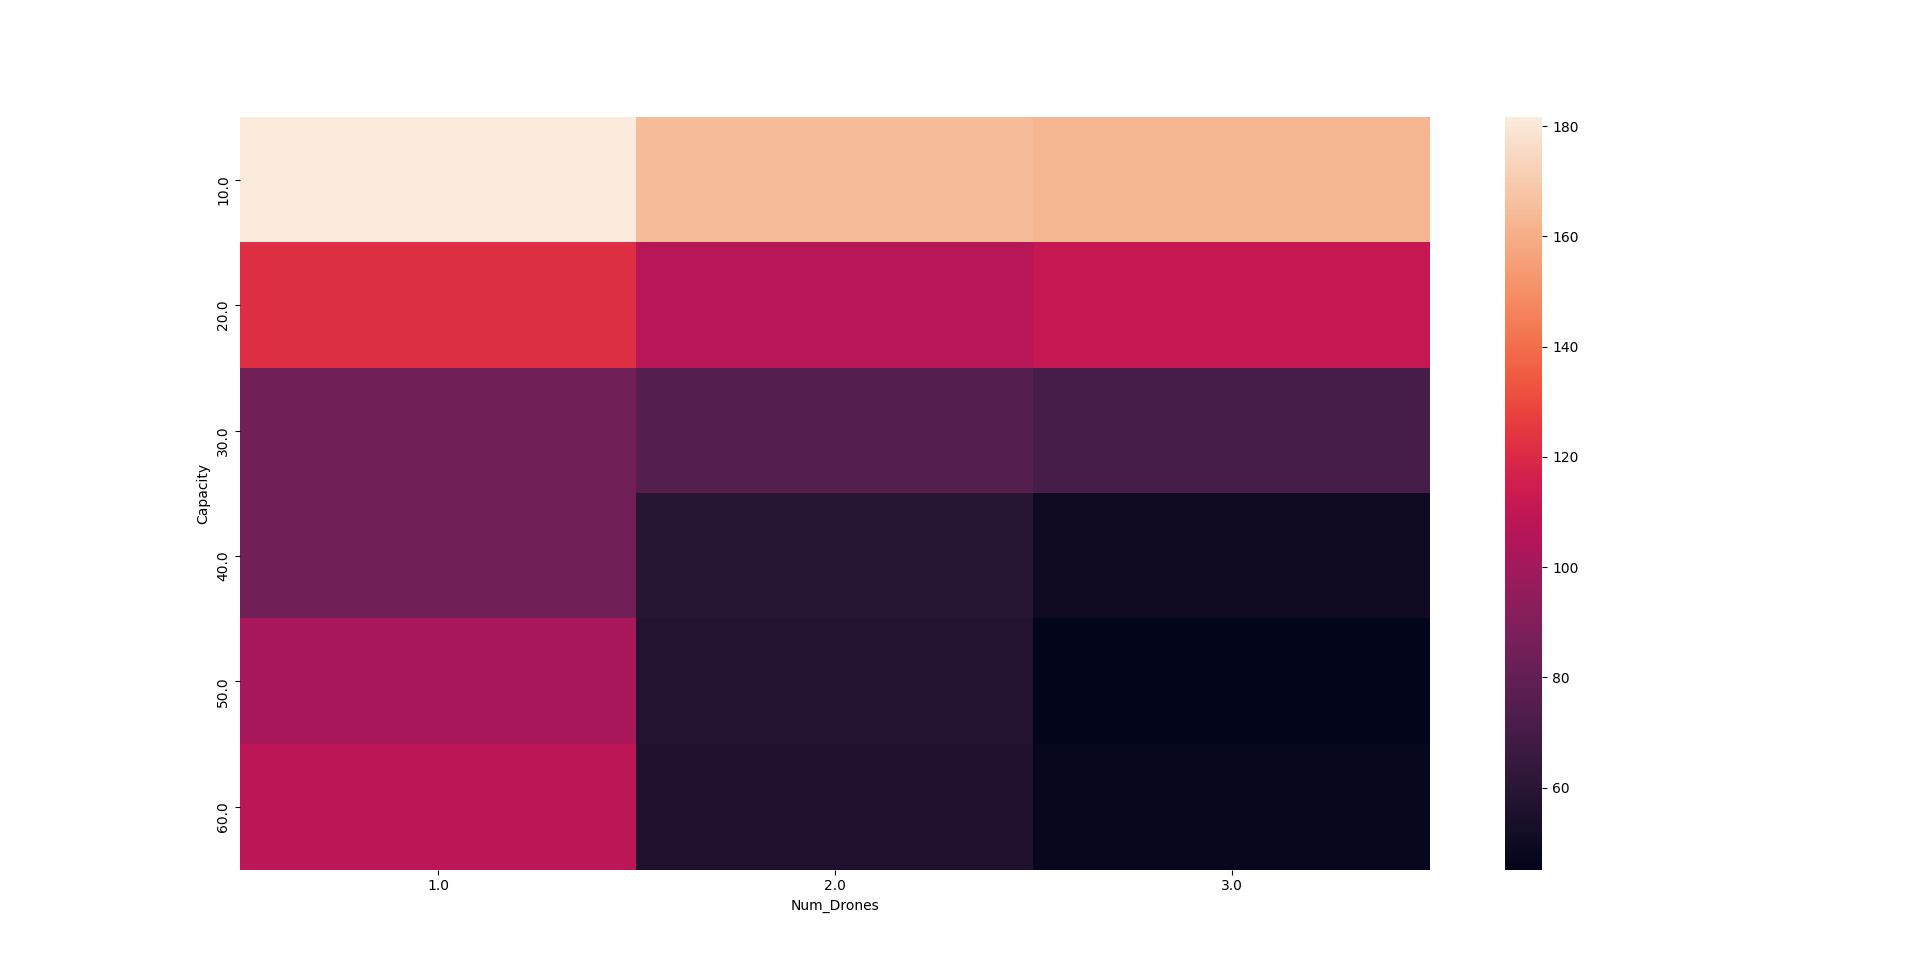
\includegraphics[width=\linewidth]{heatmap.png}
\caption{Heatmap of objective function values depending on number of drones and drone capacities. The darker the color intensity the smaller the objective value. \label{fig:heatmap}}
\end{figure}
\noindent
%In order to test the performances of the matheuristic proposed in Section \ref{Math}, we coded it in Python and we run it on the same sets of instances (Grid and Delaunay) on which the three formulations have been solved. Table \ref{table:tab3} reports for each instance, numbered from 0 to 4, distinguishing between Grid and Delauney, respectively, the best objective function provided by the best formulation, the objective function provided by the matheuristic and the associated CPU time. As already noticed from Table \ref{table:tab2}, for grid graph instances, SEC formulation has the best behaviour, with the exception of the instance number 3 for which the MTZ provides a smaller value of the objective function. As for the Delaunay graph instances, MTZ is the best formulation, but also in this case there is an exception on the instance number 2 for which SEC formulation returns a smaller value of the objective function.\\
%The results show that the matheuristic returns a solution with value of the objective function that is higher than the one provided by the SEC formulation on grid instances. However, these values are smaller than the ones provided by the Stages and the MTZ formulations. Moreover, the saving in terms of resolution time is very significant as the maximum CPU time is less than 1 minute.  As regards the Delaunay instances, the matheuristic performances are even better, as it finds a solution that is better than the best one provided by the MTZ formulation and in a resolution time that is at most 28 minutes. 



%\renewcommand{\arraystretch}{0.7}
%\begin{table}[!h]
%\caption{Heuristic performances}
%\centering
%\footnotesize
%\begin{tabular}{c | c c c | c c c}
%\hline
%\textbf{\#}  & \multicolumn{3}{c}{\textbf{Grid}} &  \multicolumn{3}{c}{\textbf{Delauney}} \\
 % \hline
% &Best Obj & Obj Heuristic &CPU Time &Best Obj & Obj Heuristic & CPU Time \\
%\hline
%0 &	1087,87	& 1117,83 &	50,99 &	947,01 &	934,46 &	52,49\\
%1 &	1100,38	& 1319,64 &	24,64 &	986,22 &	 938,68	& 72,73\\
%2 &	1350,67	& 1126,35 &	46,06 &	888,48 &	865,66 &	1073,80\\
%3 &	1218,66	& 1476,36 &	27,18 &	1249,69 &	1154,62 &	1703,33\\
%4 &	1297,77	& 1424,37 &	40,91 &	1239,93	 & 1184,67 &	81,15\\
%    \hline
%\end{tabular}
%\label{table:tab3}
%\end{table}


\noindent
%We performed a second set of experiments by observing that, even if there are small differences between the SEC and the MTZ formulations depending on the type of instances, their performances are comparable.
%Thus, in the rest of the tests we focused on the MTZ formulation. We compared its performances, with or without providing the initial solution found by the matheuristic, on a set of larger instances. More precisely, we generated 20 instances with targets represented by grid graphs and 20 instances with targets represented by Delauney graphs. The instances of each typology are split in 4 groups of 5 instances each, consisting respectively of 5, 10, 15 and 20 targets to be visited.
%In each instance the same percentage of graphs ($20\%$) has respectively 4, 6, 8, 10 and 12 nodes. 
%Moreover, we assumed that the origin coincides with the destination in all instances and we randomly generated with uniform distribution between 0 and 1, two values representing the percentage of each edge and of each graph to be visited.
%As regards the speeds, we set the speed of the drone three times the one of the mothership.
%We run the MTZ formulation by adopting Gurobi, setting a time limit of 7200 sec. for each instance.
%On the same instances also the matheuristic has been applied. Note that, in order to define a stopping rule for the exact resolution of the AMDRPG model within the matheuristic procedure (STEP 3 and STEP 4), we set the maximum number of solutions generated by the solver equal to five.
%For each instance, the solution provided by the matheuristic has been then used to initialize the exact resolution of the MTZ formulation in order to try to speed up the resolution process.
%Table \ref{table:tab4} shows the results of the comparison between the exact resolution of the formulation with and without initialization. In the first column, named List, we report the size of the instances in terms of number of targets to be visited (0, 1, 2 and 3 identifies instances respectively with 5, 10, 15 and 20 graphs).The second column refers to the two variants of the model, that is, a given percentage of each edge of the targets (e) or a given percentage of each target (g) must be visited by the drone. The other columns report respectively the average percentage gap of the solutions found within the time limit starting from the initial solution provided by the matheuristic, the average running time of the matheuristic and the average percentage gap of the solutions found within the time limit without initialization. These information are reported for both Grid and Delauney instances.

%\renewcommand{\arraystretch}{0.7}
%\begin{table}[!h]
%\caption{Comparison between exact resolution with and without initialization}
%\centering
%\footnotesize
%\begin{tabular}{c c | c c c | c c c}
%\hline
% &  & \multicolumn{3}{c}{\textbf{Grid}} &  \multicolumn{3}{c}{\textbf{Delauney}} \\
%\hline
% List &  $\%$  & $\%$ Gap (i) & Time$\_$h & $\%$ Gap (ni)  & $\%$ Gap (i) & Time$\_$h &  $\%$ Gap (ni)\\
%\hline
%\multirow{}{}{0} & e & 0.72 & 105.12 & 0.73 & 0.78 & 154.92 & 0.74\\
%& g & 0.55 & 58.92 & 0.54 & 0.62 & 92.64 & 0.67\\
%\hline
%\multirow{}{}{1} & e & 0.76 & 241.99 & 0.76 & 0.80 & 314.69 & 0.79\\
%& g & 0.71 & 182.61 & 0.70 & 0.74 & 353.04 & 0.75\\
%\hline
%\multirow{}{}{2} & e & 0.76 & 367.69 & 0.76 & 0.80 & 447.61 & 0.80 \\
%& g & 0.71 & 326.49 & 0.72 & 0.76 & 429.16 & 0.76\\
%\hline
%\multirow{}{}{3} & e & 0.75 & 481.68 & 0.74 & 0.80 & 514.98 & 0.76^*\\
%& g & 0.71 & 492.27 & 0.70 & 0.77 & 582.90 & 0.77\\
%    \hline
%\end{tabular}
%\label{table:tab4}
%\end{table}

\noindent
%From Table \ref{table:tab4} we can notice that in most of the cases the average gaps associated with the solution found within the time limit, with and without initialization by the solution found by the matheuristic, are the same or very close (note that in the last column the $*$ indicates that only one instance has been solved within the time limit).
%As regards the running time of the matheuristic, we can see also from the boxplots in Figure \ref{fig:1}, that it increases with the number of targets to be visited both for Grid and Delaunay instances. Considering the model variants based on the minimum percentage of each edge or each graph to visit, we can observe that for Grid instances the average running time of the model imposing a minimum percentage of each edge to be visited, is greater than the one associated with the other variant, with the exception of the instances of biggest size (List=3). \\
\noindent
%The boxplots in Figure \ref{fig:2} represent the percentage gap of the solution provided by the matheuristic with respect to the one provided by the exact resolution of the MTZ model within the time limit, with initialization by the solution found by the matheuristic. From them we can notice that the gap increases with the size both for Grid and Delaunay instances but it is always less than 0.5$\%$.  
%Figure \ref{fig:3} shows the percentage gap of the solution provided by the exact resolution of the MTZ formulation within the time limit without the initialization, with respect to the one found with the initialization. This gap is very close to 0 both for Grid and Delaunay instances. Only for the biggest size we observe values ranging between 0.1$\%$ and 0.6$\%$. These observations suggest that, even if the initialization of the model by the solution provided by the matheuristic does not speed up the convergence to the optimal solution, the matheuristic provides solutions of very good quality. Indeed, it generates in less than 10 minutes solutions that are very close to the ones provided by the model within 2 hours.\\


%\begin{figure}[htp]% [H] is so declass\'e!
%\centering
%\begin{minipage}{0.45\textwidth}
%\includegraphics[width=\textwidth]{time_h.png}
%\caption{Matheuristic running time}
%\label{fig:1}
%\end{minipage}\hfill
%\begin{minipage}{0.45\textwidth}
%\includegraphics[width=\textwidth]{improved_gap.png}
%\caption{Matheuristic improved gap}
%\label{fig:2}
%\end{minipage}\par
%\vskip\floatsep% normal separation between figures
%\includegraphics[width=0.45\textwidth]{differencewithwithout.png}
%\caption{Improved gap of MTZ formulation with and without initialization}
%\label{fig:3}
%\end{figure}



%\noindent
%As regards the \NMD \xspace problem, we generated three sets of instances with targets represented by grid graphs considering different structures of the polygonal network where the mothership can move.
%In particular, we defined a first set of instances where the mothership network is represented by a graph of 6 nodes with a tree structure with origin of the path of the base vehicle different from the destination.
%A second set of instances involving a mothership network consisting in a complete graph of 4 vertices with origin of the path of the base vehicle different from the destination.  
%A third set of instances characterized by star graphs of 7 nodes representing the mothership network, where the origin coincides with the destination and it is located at the centre of the star. We generated 10 instances for each of these three classes, 5 of them with 5 targets and 5 with 10 targets to be visited. 
%Moreover, as for the AMDRPG, for each of these 10 instances we randomly generated two values representing the percentage of each edge and of each graph that must be visited by the drone.
%We run on these sets of instances both Stages and MTZ formulations. Table \ref{table:tab5} summarizes the results obtained comparing them. The first column identifies the size of the instances, similarly to Table \ref{table:tab4}, (0 for instances with 5 targets and 1 for instances with 10 targets).
%The second column distinguishes between minimum percentage of each edge (e) or of each graph (g) to be visited by the drone.
%The remaining columns refer to the three different class  of instances described above (1 for the networks with a tree structure, 2 for complete networks and 3 for start networks).
%For each of these sets of instances the average percentage gap of the solutions found within the time limit of 7200 sec. by the two formulations (Stages and MTZ) is reported.


%\renewcommand{\arraystretch}{0.7}
%\begin{table}[!h]
%\caption{Comparison between formulations of \NMD}
%\centering
%\footnotesize
%\begin{tabular}{c c | c c | c c | c c}
%\hline
% & Net Struct  & \multicolumn{2}{c}{1} &  \multicolumn{2}{c}{2}  & \multicolumn{2}{c}{3}\\
%\hline
%List & $\%$ &  Stages  & MTZ & Stages & MTZ  & Stages & MTZ\\
%\hline
%\multirow{}{}{0} & e & 0.89 & 0.33 & 0.88 & 0.24 & 0.87 & 0.39\\
%& g & 0.86 & 0.29 & 0.89 & 0.18 & 0.90 & 0.42\\
%\hline
%\multirow{}{}{1} & e & 0.92 & 0.43 & 0.92 & 0.33 & 0.92 & 0.46\\
%& g & 0.91 & 0.36 & 0.92 & 0.23 & 0.92 & 0.39\\
%\hline
%\end{tabular}
%\label{table:tab5}
%\end{table}

\noindent
%We can observe that for each class of instances and model variants, based on the percentage of each edge or each graph to be visited, the MTZ formulation performs better than the Stages one. In all the cases the percentage average gap associated with the MTZ formulation is one third or half of that associated with the Stages formulation. For this reason, in the following tests, related to the comparison between the exact resolution of the \NMD\xspace  model with and without the initialization by the solution found by the matheuristic, we focused only on the MTZ formulation.\\
%Table \ref{table:tab6} summarizes the results of this comparison distinguishing again between the different network structures (columns labelled 1, 2 and 3), the different size (rows labelled 0 and 1) characterizing the instances and model variants (minimum percentage of each edge (e) or each graph (g) to be visited). For each combination of network structure, size and model variant we reported the average percentage gap with initialization ($\%$ Gap (i)), the solution time of the matheuristic (T$\_$h) and the average percentage gap without initialization by the solution found by the matheuristic ($\%$ Gap (ni))

%\renewcommand{\arraystretch}{0.8}
%\begin{table}[!h]
%\caption{Comparison between exact resolution with and without initialization of \NMD}
%\centering
%\scriptsize
%\begin{tabular}{c c | c c c | c c c | c c c}
%\hline
% & Net Struct  & \multicolumn{3}{c}{1} &  \multicolumn{3}{c}{2}  & \multicolumn{3}{c}{3}\\
%\hline
%List &  $\%$  & $\%$ Gap (i) & T$\_$h & $\%$ Gap (ni)  & $\%$ Gap (i) & T$\_$h &  $\%$ Gap (ni) & $\%$ Gap (i) & T$\_$h &  $\%$ Gap (ni)\\
%\hline
%\multirow{}{}{0} & e & 0.32 & 109.96 & 0.33 & 0.24 & 207 & 0.24 & 0.39 & 177.57 & 0.39\\
%& g & 0.30 & 110.92 & 0.29 & 0.18 & 163.36 & 0.18 & 0.45 & 149.68 & 0.42\\
%\hline
%\multirow{}{}{1} & e & 0.48 & 1030.64 & 0.43 & 0.39 & 802.3 & 0.33 & 0.53 & 770.05 & 0.46\\
%& g & 0.33 & 479.36 & 0.36 & 0.35 & 639.09 & 0.23 & 0.42 & 689.51 & 0.39\\
%\hline
%\end{tabular}
%\label{table:tab6}
%\end{table}

\noindent
%We can observe that, similarly to the AMDRPG problem, the average gaps associated with the solution found within the time limit, with and without initialization by the solution found by the matheuristic, are very close. Considering the average running time we can notice that the \NMD\xspace  problem is more challanging to be solved with respect to the AMDRPG. It increases very fast with the size of the instances especially for the case in which the network where the mothership moves has a tree structure. Moreover, as for the Grid instances in the continuous case, the model variant imposing a minimum percentage of each edge to be visited takes more time to be solved.

%\begin{figure}
%\centering
%\includegraphics[width=5cm]{improved_gap_ND.png}
%\caption{Matheuristic improved gap for \NMD}
%\label{fig:4}
%\end{figure}
\noindent
%The boxplots showed in Figure \ref{fig:4} report the percentage gap of the solution provided by the matheuristic with respect to the one provided by the exact resolution of the MTZ model within the time limit, with initialization by the solution found by the matheuristic.
%We can notice that, excluding the outliers, this gap ranges between 0$\%$ and 0.7$\%$ and its lowest values are observed for the instances in which the network where the mothership moves has a star structure (green boxplots). 
%From the previous observations, similarly to the AMDRPG, we can conclude that the behaviour of the matheuristic is very good in terms of quality of the solutions provided, even if the initialization of the MTZ model does not help in speeding up the convergence to the optimal solution. 












%\section{Case Study\label{section:CS}}

\noindent
In this section\CV{,} we describe a realistic application of the system studied in this paper to perform surveillance operations. Considering the current COVID-19 restrictions, we focus on the problem of preventing and identifying possible concentrations of people during events such as popular or religious festivals. In particular\CV{,} we consider the Courtyards Festival of Cordoba (\url{https://patios.cordoba.es/es/}). This is a social event that takes place every year in the city of Cordoba, Spain, during the first two weeks of May. Courtyard’s owners decorate their houses with many flowers trying to win the award that is offered by the Town Hall. During this competition\CV{,} a festival runs in parallel with a number of artistic performances along six different paths located in different areas in the city as shown in Figure \ref{fig:mapPF}.
In the pandemic context, to monitor the situation to avoid \CV{the} concentration of people, we propose to apply a system consisting of one helicopter and a fleet of three drones.
This kind of system has been proved successfully and has been already applied in the military field by the US Army (in order to) \CV{to} leave the helicopter (to) \CV{at} the edge of dangerous airspace and release drones, which will then penetrate \CV{the} enemy territory and send back intelligence, surveillance and reconnaissance information (see \cite{FG}).
In our application\CV{,} the reason to adopt a similar system is the possibility to inspect simultaneously and in real time different paths\CV{,} also reducing the risk of flying the helicopter over populated areas and the cost (for) \CV{of} moving the helicopter by minimizing the total length of its tour.

\begin{figure}[h!]
\centering
\includegraphics[width=0.6\linewidth]{figures/first.png}
\caption{Map of the Courtyards Festival in Cordoba. \label{fig:mapPF}}
\end{figure}

\noindent
We run the model presented in Section \ref{Form} on this scenario starting from the initial solution provided by the matheuristic, where the 6 coloured paths reported in the map of Figure \ref{fig:mapPF} represent the 6 target graphs to be visited, in this case inspected, by the fleet of drones. In addition, we suppose that the drones' speed is \LA{43} km/h while that of the helicopter is  \LA{30} km/h aiming to minimize costs.
Moreover, we assume that the fleet is composed by \LA{two} drones with an endurance equal to \LA{30 minutes}, and we impose that each target graph must be fully visited (inspected).  As we can see from Figure \ref{fig:Mtour}, the origin of the mothership tour coincides with the destination and it is located in an area of the city where it is possible to assume the take-off and landing of an helicopter. Figure \ref{fig:Mtour} reports the tour followed by the helicopter \CV{with} (in) the solution obtained within the time limit of 2 hours \CV{set(s)} to solve the model and with a percentage gap equal to 83\%. We can observe that the helicopter, starting from the origin, flies to the point $x_L^1$ that is the first launching point and then flies along the edge connecting $x_L^1$ with $x_R^1$, that is the first rendezvous point. Next, the helicopter flies to $x_L^2$ for launching the second drones' mission that are retrieved at point $x_R^2$. The third and last mission starts from $x_L^3$ and ends at point $x_R^3$ from where the helicopter goes back to the final destination.\\
Figure \ref{fig:tourD} shows the tour followed by the three drones for inspecting the six paths. In particular, one drone, in red, starts from $x_L^1$ for visiting the path of "Alcazar Viejo". From the same point\CV{,} a second drone, in green, starts for visiting the path of "Santa Maria-San Agustin". Both drones end their first mission at point $x_R^1$, where they are retrieved by the helicopter. Then, the helicopter flies to point $x_L^2$ where only one drone, the red one, starts its second mission to visit the path of "Juderia-San Francisco". In the meanwhile\CV{,} the helicopter, containing the other two drones, flies to point $x_R^2$ where it retrieves the previously launched drone. The last mission involves all the three drones that are launched from point $x_L^3$. The first drone, the red one, visits the path of "San Lorenzo", the second, the green one, visits the path of "Regina-Realejo" and the third, the blue one, visits the path of "Santiago-San Pedro".
All the three drones are retrieved by the helicopter at point $x_R^3$ and after that the helicopter goes back to the destination. 
The total distance travelled by the helicopter is equal to 11.27 km.

All details of this case study, including map coordinates, .lp models and solutions can be found in \cite{Puerto2021}.


\begin{figure}[h!]
\centering
\includegraphics[width=0.6\linewidth]{figures/second.png}
\caption{Mothership tour. \label{fig:Mtour}}
\end{figure}

\begin{figure}[h!]
\centering
\includegraphics[width=0.6\linewidth]{figures/third.png}
\caption{The complete solution. \label{fig:tourD}}
\end{figure}
\section{Case Study\label{section:CS}}

\noindent
In this section\CV{,} we describe a realistic application of the system studied in this paper to perform surveillance operations. Considering the current COVID-19 restrictions, we focus on the problem of preventing and identifying possible concentrations of people during events such as popular or religious festivals. In particular\CV{,} we consider the Courtyards Festival of Cordoba (\url{https://patios.cordoba.es/es/}). This is a social event that takes place every year in the city of Cordoba, Spain, during the first two weeks of May. Courtyard’s owners decorate their houses with many flowers trying to win the award that is offered by the Town Hall. During this competition\CV{,} a festival runs in parallel with a number of artistic performances along six different paths located in different areas in the city as shown in Figure \ref{fig:mapPF}.
In the pandemic context, to monitor the situation to avoid \CV{the} concentration of people, we propose to apply a system consisting of one helicopter and a fleet of \LA{two} drones.
This kind of system has been proved successfully and has been already applied in the military field by the US Army to leave the helicopter at the edge of dangerous airspace and release drones, which will then penetrate \CV{the} enemy territory and send back intelligence, surveillance and reconnaissance information (see \cite{FGA}).
In our application\CV{,} the reason to adopt a similar system is the possibility to inspect simultaneously and in real time different paths\CV{,} also reducing the risk of flying the helicopter over populated areas and the cost of moving the helicopter by minimizing the total length of its tour.

\begin{figure}[h!]
\centering
\includegraphics[width=0.6\linewidth]{first.png}
\caption{Map of the Courtyards Festival in Cordoba. \label{fig:mapPF}}
\end{figure}

\noindent
We run the \LA{models} presented in Section \ref{Form} on this scenario starting from the initial solution provided by the matheuristic, where the 6 coloured paths reported in the map of Figure \ref{fig:mapPF} represent the 6 target graphs to be visited, in this case inspected, by the fleet of drones. In addition, we suppose that the drones' speed is \LA{43} km/h while that of the helicopter is  \LA{30} km/h aiming to minimize costs.
Moreover, we assume that the fleet is composed by \LA{two} drones with an endurance equal to \LA{7.5 minutes}, and we impose that each target graph must be fully visited (inspected).  As we can see from Figure \ref{fig:Mtour_CO} and Figure \ref{fig:Mtour_PO}, the origin of the mothership tour coincides with the destination and it is located in an area of the city where it is possible to assume the take-off and landing of an helicopter. Figure \ref{fig:Mtour_CO} reports the tour followed by the helicopter \LA{in} the solution \LA{of the complete overlapping version of the problem}, after \CV{4} hours of running time. We can observe that the helicopter, starting from the origin, flies to the point $x_R^1$ that is the first \LA{rendezvous} point, \LA{coinciding with the second launching point $x_L^2$}. Then, it flies along the edge connecting $x_R^1$ with $x_R^2$, that is the second rendezvous point, \LA{which coincides with the third launching point $x_L^3$}. Next, the helicopter flies to \LA{$x_R^3$ for retrieving the third drones' mission. From the same point the fourth and last mission starts and ends at point $x_R^4$, that is also the final destination of the helicopter tour.}\\
Figure \ref{fig:tourD_CO} shows the tour followed by the \LA{two} drones for inspecting the six paths. In particular, \LA{one drone, in red, starts from the origin ($origin=x_L^1$) for visiting the path of "Alcazar Viejo". It is retrieved by the helicopter at point $x_R^1$ and from the same point both drones, in red and blue, are launched to visit respectively the paths of "Juderia-San Francisco" and "Santa Maria-San Agustin". Both drones end their mission at point $x_R^2$. From this latter point they are launched to perform the visits to the paths of "San Lorenzo" and "Regina-Realejo". Then, they are both retrieved by the  helicopter at point $x_R^3$ where only one drone, the red one, starts its last mission to visit the path of "Santiago-San Pedro". In the meanwhile, the helicopter, containing the other drone (the blue one), flies to point $x_R^4=dest$ where it retrieves the red drone and ends its tour.}
The total time travelled by the helicopter is around 21 minutes.
\LA{We can observe that in the drone tour on "San Lorenzo" and "Regina-Realejo" graphs, there are two edges whose duplicate is represented with a dotted segment in Figure \ref{fig:tourD_CO}. They are associated with edges of the graph that are visited once, but travelled twice by the drone, in order to perform the inspection of the whole graph.\\
Figure \ref{fig:Mtour_PO} shows the mothership tour in the solution of the partial overlapping version of the problem, always obtained by setting a time limit of \CV{4} hours. In this case, we can observe that the helicopter follows a different tour and that there are more launching and retrieving points due to the possibility of launching a drone before retrieving the other one. From Figure \ref{fig:tourD_PO} we can see that, differently from the complete overlapping version, both drones start their first mission from the origin $origin=x_L^1=x_L^2$. The red drone visits the path of "Alcazar Viejo", while the blue one visits the path of "Santiago-San Pedro". The red drone is retrieved by the helicopter at point $x_R^3$ and it is launched again from the point $x_L^4$. From this latter point the red drone starts its second mission to visit the path of "Juderia-San Francisco". In the meantime, the helicopter flies to the point $x_R^5$ where the blue drone is retrieved. From the same point $x_R^5=x_L^6$ the blue drone is then launched to inspect the path of "Santa Maria-San Agustin". Both drones are retrieved by the helicopter at the point $x_R^7=x_R^8$ (shown in pink colour in Figure \ref{fig:tourD_PO}). From this latter point $x_R^8=x_L^9$ the red drone is launched to visit the path of "Regina-Realejo". Then, the helicopter flies to the point $x_L^{10}$ from where the blue drone starts its last visit to the path of "San Lorenzo". Finally, the helicopter flies to the destination $dest$ and along its path, it retrieves first the red drone at the point $x_R^{11}$ and then the blue one at the point $x_R^{12}$. Also in this case, like in the solution of the complete overlapping version of the problem, we have one edge of the graph associated with the path of "Regina-Realejo" and one edge of the graph representing the path of "San Lorenzo", that are traversed twice represented with dotted segments in Figure \ref{fig:tourD_PO}. The total travel time of the helicopter is 19 minutes. It is slightly lower than the one associated with the solution of the complete overlapping version of the problem. Thus, even if on this scenario we cannot observe big changes in terms of the objective function value, we can see how the different assumptions associated with the two versions of the problem can influence the structure of the solution, by producing a different schedule of the drone missions and a different location of the launching and rendezvous points.}\\
\noindent
All details of this case study, including map coordinates, .lp models and solutions can be found in \cite{Puerto2021}.


\begin{figure}[h!]
\centering
\includegraphics[width=0.6\linewidth]{synchronous_1.png}
\caption{Mothership tour (CO) \label{fig:Mtour_CO}}
\end{figure}
\begin{figure}[h!]
\centering
\includegraphics[width=0.6\linewidth]{synchronous_2.png}
\caption{The complete solution (CO) \label{fig:tourD_CO}}
\end{figure}

\begin{figure}[h!]
\centering
\includegraphics[width=0.6\linewidth]{asynchronous_1.png}
\caption{Mothership tour (PO) \label{fig:Mtour_PO}}
\end{figure}
\begin{figure}[h!]
\centering
\includegraphics[width=0.6\linewidth]{asynchronous_2.png}
\caption{The complete solution (PO) \label{fig:tourD_PO}}
\end{figure}
%\section{Concluding remarks}
\noindent
This papers has analyzed the coordination problem that arises between a mothership vehicle and a fleet of drones that must coordinate their routes to minimize the total distance travelled by the mothership while visiting a set of targets modeled by graphs. We have presented exact formulations of the problem, for its synchronized and not synchronized versions. They are mixed integer non-linear programming models. Moreover, we presented valid inequalities for them. \\
Our computational results show that the considered problem is very challenging to solve even on small to medium size instances. For that reason, additionally, we have proposed a matheuristic algorithm that provides acceptable feasible solutions in very short computing time; so that it is a good alternative to the exact method. We report extensive computational experiments on randomly generated instances. Moreover, we present a case study related to inspection activities in the context of COVID-19 restrictions. We show the application of the system described in this paper in the framework of the Courtyard Festival in the city of Cordoba, by illustrating the solution obtained by adopting the problem formulation, in its synchronized version, and its solution by means of the initialization provided by the proposed matheuristic.\\
\noindent
The formulation and algorithms proposed in this paper can be seen a first building block to handle coordination of systems given by a base vehicle and drones. Further research in this topic must focus on finding faster and more accurate algorithms able to solve larger instances. Moreover, it is also challenging to model more complex operations  allowing that drones can visit more than one target per trip. These problems being very interesting are beyond the scope of the present paper and will be the focus of a follow up research line.
\section{Concluding remarks\label{section:CR}}
\noindent
This paper has analyzed the coordination problem that arises between a mothership vehicle and a fleet of drones that must coordinate their routes to minimize the total time traveled by the mothership while visiting a set of targets modeled by graphs. We have presented exact mixed integer nonlinear programming formulations of the problem for its complete and partial overlapping versions. Moreover, we strengthen the models with some valid inequalities for them. \\
Our computational results show that the considered problem is very challenging to solve even on small and medium size instances. For that reason, additionally, we have proposed a matheuristic algorithm that provides good quality feasible solutions in a short computing time; so that it is a good alternative to the exact method. We report extensive computational experiments on randomly generated instances. Moreover, we present a case study related to inspection activities in the context of COVID-19 restrictions. We show the application of the system described in this paper in the framework of the Courtyard Festival in the city of Cordoba, by illustrating the solution obtained by adopting the problem formulation, in both versions of the model, and its solution by means of the initialization provided by the proposed matheuristic.\\
\noindent
The formulation and algorithms proposed in this paper can be seen \JP{as} a first building block to handle the coordination of systems \JP{composed by a base vehicle and a number of  drones.} Further research in this topic must focus on finding faster and more accurate algorithms able to solve larger size instances. Moreover, it is also challenging to model more complex operations allowing that drones can visit more than one target per trip. Other extensions that may be considered can take into account that the time spent by the mothership to launch and retrieve the drones is not negligible as well as \JP{handling the speed of the mothership and drones as decision variables}. These problems being very interesting are beyond the scope of the present paper and will be the focus of a follow up research line.
\section*{Acknowledgements}
This research has been partially supported by Spanish Ministry of Education and Science/FEDER grant number  PID2020-114594GB02, and projects Junta de Andalucia P18-FR-1422, FEDER-US-1256951, CEI-3-FQM331 and  \textit{NetmeetData}: Ayudas Fundaci\'on BBVA a equipos de investigaci\'on cient\'ifica 201%\section{Introduction}

% \bibliographystyle{apa}

\bibliographystyle{elsarticle-num-names}
% \printbibliography

\bibliography{bibliography2.bib}
%\section{Appendix}\label{App}
\noindent
In this section, we report an extension of the MINLP formulation presented in Section \ref{Form}, for dealing with the case of nonhomogeneous fleets of drones.
\noindent
In the following, we introduce the parameters or input data that formally describe the problem and that are summarized in Table \ref{table:At1}.
\noindent
\JP{The formulation in this appendix is rather similar to the one in Section \ref{subsec:CO} but, because of the assumption of nonhomogeneous drones, it needs to keep track of the drones used in each action. This implies to include an extra index $\delta$ in most of the variables. For the sake of completeness, we have included the complete set of constraints of this formulations although some of them are similar to those in Section \ref{subsec:CO}. Table \ref{table:At2} summarizes all the decision variables used in this formulation.}

\begin{table}[!h]
\scriptsize
\centering
%\color{blue}
\begin{tabular}{ | l | }
\hline
\textbf{Problem Parameters}\\
\hline
$orig$: coordinates of the point defining the origin of the mothership path (or tour).\\
$dest$: coordinates of the point defining the destination of the mothership path (or tour).\\
$\mathcal{G}$: set of the target graphs.\\
$g = (V_g, E_g)$: set of nodes and edges of each target graph $g \in \mathcal{G}$.\\
$\mathcal{L}(e_g)$: length of edge $e$ of graph $g \in \mathcal{G}$.\\
$\mathcal{L}(g)=\sum_{e_g\in E_g} \mathcal L(e_g)$: total length of the graph $g\in\mathcal G$.\\
$B^{e_g}, C^{e_g}$: coordinates of the endpoints of edge $e$ of graph $g \in \mathcal{G}$.\\
$\alpha^{e_g}$: fraction of edge $e$ of graph $g \in \mathcal{G}$ that must be visited.\\
$\alpha^{g}$: fraction of graph $g \in \mathcal{G}$ that must be visited.\\
$v_M$: mothership speed.\\
$\mathcal D$: set of drones.\\
$v_\delta$: drone $\delta$ speed.\\
$N_\delta$: drone $\delta$ endurance. \\
$\mathcal{O}$: set of drones operations to perform visits to the target graphs\\
$M$: big-M constant.\\
\hline
\end{tabular}
\caption{Nomenclature for AMMDRPG with non-homogeneous fleet of drones}
\label{table:At1}
\end{table}

\begin{table}[h!]
%\tiny
\scriptsize
\centering
%\color{blue}
\begin{tabular}{|l|}
\hline 
\textbf{Binary and Integer Decision Variables}\\
\hline
$\mu^{e_g} \in \{0,1\}, \:\: \forall e_g \in E_g\:\: (g \in \mathcal{G})$: equal to 1 if edge $e$ of graph $g$ (or a fraction of it) is visited by the drone, 0 otherwise.\\
$\text{entry}^{e_g} \in \{0,1\}, \:\: \forall e_g \in E_g\:\: (g \in \mathcal{G})$: auxiliary binary variable used for linearizing expressions.\\
$u^{e_{g}o\delta} \in \{0,1\}, \:\: \forall e_g \in E_g\:\: (g \in \mathcal{G}), \:\:\forall o \in \mathcal O, \:\: \forall \delta \in \mathcal D$: equal to 1 if the drone $\delta$ enters in graph $g$ by the edge $e_g$ at operation $o$,\\ \hspace*{1cm} 0 otherwise.\\
$z^{e_{g}e^{'}_{g}} \in \{0,1\}, \:\: \forall e_g, e_g' \in E_g\:\: (g \in \mathcal{G})$: equal to 1 if the drone goes from $e_g$ to $e^{'}_{g}$, 0 otherwise.\\
$v^{e_{g}o\delta} \in \{0,1\}, \:\: \forall e_g \in E_g\:\: (g \in \mathcal{G}), \:\: \forall o \in \mathcal O, \:\: \forall \delta \in \mathcal D$: equal to 1 if the drone $\delta$ exits from graph $g$ by $e_g$ at operation $o$,\\ \hspace*{1cm} 0 otherwise.\\
\hline
\textbf{Continuous Decision Variables}\\
\hline
$s^{e_g}\in[0, |E_g|-1],\:\: \forall e_g \in E_g\:\: (g \in \mathcal{G})$: continuous non negative variable representing the order of visit of the edge $e$ of graph $g$.\\
$\rho^{e_g} \in [0,1]$ and $\lambda^{e_g} \in [0,1], \:\: \forall e_g \in E_g\:\: (g \in \mathcal{G})$: defining the entry and exit points on $e_g$.\\
$\nu_\text{min}^{e_g}$ and $\nu_\text{max}^{e_g} \in [0,1], \:\: \forall e_g \in E_g\:\: (g \in \mathcal{G})$: auxiliary variables used for linearizing expressions.\\
$p^{e_g}\in [0, 1], \:\: \forall e_g \in E_g\:\: (g \in \mathcal G)$: auxiliary variable used for modelling the product of $\mu^{e_g}$ and $|\lambda^{e_g}-\rho^{e_g}|$.\\
$x_L^o\in\mathbb R^2, \:\: \forall o \in \mathcal O$: coordinates representing the point where the mothership launches the drones at operation $o$.\\
$x_R^o\in\mathbb R^2, \:\: \forall o \in \mathcal O$: coordinates representing the point where the mothership retrieves the drones at operation $o$.\\
$R^{e_g}\in\mathbb R^2, \:\: \forall e_g \in E_g\:\: (g \in \mathcal{G})$: coordinates representing the entry point on edge $e_g$ of graph $g$.\\
$L^{e_g}\in\mathbb R^2, \:\: \forall e_g \in E_g\:\: (g \in \mathcal{G})$: coordinates representing the exit point on edge $e_g$ of graph $g$.\\
$d_L^{e_go\delta} \geq 0, \:\: \forall e_g \in E_g\:\: (g \in \mathcal{G}),\:\: \forall o \in \mathcal O, \:\: \forall \delta\in\mathcal D$: representing the distance travelled by the drone $\delta$ from the launching\\
\hspace*{1cm} point $x_L^o$ on the mothership at operation $o$ to the first visiting point $R^{e_g}$ on $e_g$.\\
$p_L^{e_go\delta} \geq 0, \:\: \forall e_g \in E_g\:\: (g \in \mathcal{G}), \:\:\forall o \in \mathcal O, \:\:\forall \delta\in\mathcal D$: auxiliary variable used for modelling the product of $d_L^{e_go\delta}$ and $u^{e_go\delta}$.\\
$d^{e_g} \geq 0, \:\: \forall e_g \in E_g \:\: (g \in \mathcal{G})$: representing the distance travelled by the drone from the rendezvous point $R^{e_g}$ to the \\
\hspace*{1cm} launching point $L^{e_g}$ on $e_g$. \\
$d^{e_ge^\prime_g} \geq 0, \:\: \forall e_g, e^\prime_g \in E_g \:\: (g \in \mathcal{G})$: representing the distance travelled by the drone from the launching point $L^{e_g}$ on $e_g$ to\\
\hspace*{1cm}  the rendezvous point $R^{e^\prime_g}$ on $e^\prime_g$.\\
$p^{e_ge^\prime_g} \geq 0, \:\: \forall e_g, e^\prime_g \in E_g \:\: (g \in \mathcal{G})$: auxiliary variable used for modelling the product of $d^{e_ge^\prime_g}$ and $z^{e_ge^\prime_g}$.\\
$d_R^{e_go\delta} \geq 0, \:\: \forall e_g \in E_g\:\: (g \in \mathcal{G}), \:\: \forall o \in \mathcal O, \:\:\forall \delta\in\mathcal D$: representing the distance travelled by the drone $\delta$ from the last visiting point\\
\hspace*{1cm} $L^{e_g}$ on $e_g$ to the rendezvous point $x_R^o$ on the mothership at operation $o$.\\
$p_R^{e_go\delta} \geq 0, \:\: \forall e_g \in E_g\:\: (g \in \mathcal{G}), \:\:\forall o \in \mathcal O, \:\:\forall \delta\in\mathcal D$: auxiliary variable used for modelling the product of $d_R^{e_go\delta}$ and $v^{e_go\delta}$.\\
$d_{orig}\geq 0$: distance from the origin $orig$ to the first launching point $x_L^1$.\\
$d_{LR}^o \geq 0, \:\: \forall o \in \mathcal O$: representing the distance travelled by the mothership from the launching point $x_L^o$ to the rendezvous\\
\hspace*{1cm}   point $x_R^o$ at operation $o$.\\
$d_{RL}^o \geq 0, \:\: \forall o \in \mathcal O\setminus|\mathcal O|$: representing the distance travelled by the mothership from the rendezvous point $x_R^o$ at operation $o$ to the \\ 
\hspace*{1cm}  launching point $x_L^{(o+1)}$ at operation $o+1$.\\
$d_{dest}\geq 0$: distance from the last retrieving point $x_R^{|\mathcal O|}$ to the destination $dest$.\\
$time_D^o \geq 0, \:\: \forall o \in \mathcal O$: maximum time spent by a drone during operation $o$.\\
$time_M^o \geq 0, \:\: \forall o \in \mathcal O$: time spent by the mothership to go from the launching point $x_L^o$ to the retrieving point $x_R^o$ of operation $o$.\\
$time_M \geq 0$: total time spent by the mothership to go from the origin to the destination.\\
\hline
\end{tabular}
\caption{Decision Variables for AMMDRPG with non-homogeneous fleet of drones}
\label{table:At2}
\end{table}

\subsection*{Visits of graphs}
\noindent
As for the case of a homogeneous fleet of drones presented in Section \ref{Form}, to represent the movement of the drone within a graph $g\in\mathcal G$, we proceed to introduce some notation related to $g$.
Let $g = (V_g, E_g)$ be a graph in $\mathcal G$ whose total length is denoted by $\mathcal L(g)$. Here, $V_g$ denotes the set of nodes and $E_g$ denotes the set of edges connecting pairs of nodes.  Let $e_g$ be the edge $e$ of the graph $g \in G$ and let $\mathcal  L(e_g)$ be its length. Each edge $e_g$ is parameterized by its endpoints $B^{e_g}= (B^{e_g}(x_1), B^{e_g}(x_2))$ and $C^{e_g}= (C^{e_g}(x_1), C^{e_g}(x_2))$ and we can compute its length $\mathcal L(e_g) =\|C^{e_g} -  B^{e_g}\|$. 
\noindent
For each edge $e_g$ it is associated an indicator binary variable $\mu^{e_g}$ that is one if the drone visits the segment $e_g$. Moreover, we define the entry and exit points $R^{e_g}=(B^{e_g},C^{e_g},\rho^{e_g})$ and $L^{e_g}=(B^{e_g},C^{e_g},\lambda^{e_g})$ that determine the fraction of the edge visited by the drone. The coordinates of the points $R^{e_g}$ and $L^{e_g}$ are given, respectively by 
$$R^{e_g} = \rho^{e_g} B^{e_g} + (1- \rho^{e_g})C^{e_g} \quad\text{ and }\quad L^{e_g} = \lambda^{e_g} B^{e_g} + (1- \lambda^{e_g})C^{e_g},$$ where $\rho^{e_g} \in [0,1]$ and $\lambda^{e_g} \in [0,1]$ are variables to determine the position of the points on the segment.

\noindent
As discussed in Section \ref{section:desc}, we consider two modes of visit to the target graphs $g\in \mathcal{G}$:
\begin{itemize}
    \item Visiting a fraction $\alpha^{e_g}$ of each edge $e_g$ which can be modeled by using the following constraints:
    \begin{equation}\label{eq:NOalphaE}\tag{$\alpha$-E}
    |\lambda^{e_g} - \rho^{e_g}|\geq \alpha^{e_g}, \quad \forall e_g\in E_g.
    \end{equation}
    These inequalities state that the difference between the parametrizations of the entry and exit points associated to each edge $e_g$ must be higher than the fraction of the length of $e_g$ required to be traversed.
    \item Visiting a fraction $\alpha^g$ of the total length of the graph:
    \begin{equation}\label{eq:NOalphaG}\tag{$\alpha$-G}
    \sum_{e_g\in E_g} \mu^{e_g}|\lambda^{e_g} - \rho^{e_g}|\mathcal L(e_g) \geq \alpha^g\mathcal L(g).
    \end{equation}
    \noindent
    This constraint ensures that the sum of the fractions of the length of those edges chosen to be crossed must be higher than the fraction of the length of $g$ required to be traversed.
\end{itemize}



\bigskip
\noindent
In both cases, the corresponding constraints are nonlinear. To linearize them, we need to introduce a binary variable $\text{entry}^{e_g}$ that determines the traveling direction on the edge $e_g$ as well as the definition of the auxiliary variables $\nu_\text{min}^{e_g}$ and $\nu_\text{max}^{e_g}$ of the access and exit points on that segment. Then, for each edge $e_g$, the absolute value constraint \eqref{eq:NOalphaE} can be represented by:


\begin{equation}\label{eq:NOalpha-E}\tag{$\alpha$-E}
 |\rho^{e_g}-\lambda^{e_g}|\geq \alpha^{e_g} \Longleftrightarrow
 \left\{
 \begin{array}{ccl}
  \rho^{e_g} - \lambda^{e_g}                       & =    & \nu_\text{max}^{e_g} - \nu_\text{min}^{e_g},                                     \\
  \nu_\text{max}^{e_g}                         & \leq & 1-{\text{entry}^{e_g}},                                   \\
  \nu_\text{min}^{e_g}                      & \leq & {  \text{entry}^{e_g}},                                        \\
    \nu_\text{min}^{e_g}, \,\nu_\text{max}^{e_g} & \geq & 0, \\

  \nu_\text{max}^{e_g} + \nu_\text{min}^{e_g} & \geq & \alpha^{e_g}.
  \\
 \end{array}
 \right.
\end{equation}

\noindent
The first four inequalities model the standard trick of the linearization of the absolute value. The last constraint ensures that the value of the linear expression of the absolute value is higher than the required fraction $\alpha^{e_g}$.
\noindent
Similarly, \eqref{eq:NOalphaG} can be linearized as follows:
\begin{equation}\label{eq:NOalpha-G}\tag{$\alpha$-G}
 \sum_{e_g\in E_g} \mu^{e_g}|\rho^{e_g}-\lambda^{e_g}|\mathcal L(e_g)\geq \alpha^g\mathcal L(g). \Longleftrightarrow
 \left\{
 \begin{array}{ccl}
  \rho^{e_g} - \lambda^{e_g}                       & =    & \nu_\text{max}^{e_g} - \nu_\text{min}^{e_g},                                     \\
  \nu_\text{max}^{e_g}                         & \leq & 1-{\text{entry}^{e_g}},                                   \\
  \nu_\text{min}^{e_g}                      & \leq & {  \text{entry}^{e_g}},                                        \\
  \nu_\text{min}^{e_g}, \,\nu_\text{max}^{e_g} & \geq & 0, \\
  p^{e_g} & \leq & \nu_\text{max}^{e_g} + \nu_\text{min}^{e_g}, \\
  p^{e_g} & \leq & \mu^{e_g}, \\
  p^{e_g} & \geq & \nu_\text{max}^{e_g} + \nu_\text{min}^{e_g} + \mu^{e_g} - 1, \\
  \sum_{e_g\in E_g} p^{e_g}\mathcal L(e_g) & \geq & \alpha^{g}\mathcal L(g),
  \\
 \end{array}
 \right.
\end{equation}
where $p^{e_g}$ is the auxiliary variable that represents the product of the binary variable $\mu^{e_g}$ and the absolute value difference $|\rho^{e_g} - \lambda^{e_g}|$. The first four inequalities linearize again the absolute value expression. The (second) following three constraints model the product of the expression of the absolute value and the binary variable $\mu^{e_g}$. The last inequality ensures that the fraction of the length of those edges chosen to be crossed must be higher than the fraction of the length of $g$ required to be traversed.

\subsection*{Elimination of subtours}
\noindent
As already presented in Section \ref{Form},  to prevent the existence of subtours within each graph $g\in \mathcal G$ that the drone must visit, one can include, among others, either the compact formulation that uses the Miller-Tucker-Zemlin constraints (MTZ) or the subtour elimination constraints (SEC).\\
\noindent
For the MTZ formulation, we use the continuous variables $s^{e_g}$, defined in Table \ref{table:At2}, that state the order to visit the edge $e_g$ and set the following constraints for each $g\in\mathcal G$:

\begin{align}
    s^{e_g} - s^{e^\prime_g} + |E_g|z^{e_ge^\prime_g} & \leq |E_g| - 1  , &\quad\forall e_g \neq e_g'\in E_g, \tag{MTZ$_1$} \label{NOMTZ1}\\
    0 & \leq s^{e_g} \leq |E_g| - 1, &\quad\forall e_g\in E_g.\tag{MTZ$_2$}\label{NOMTZ2}
\end{align}

\noindent
Alternatively, we can also use the family of subtour elimination constraints for each $g\in\mathcal G$:
\begin{equation}\tag{SEC}\label{NOSEC}
    \sum_{e_g, e^\prime_g \in S} z_g^{e_ge^\prime_g} \leq |S| - 1, \quad \forall S\subset E_g.
\end{equation}

\noindent
To find SEC inequalities, as usual, we search for disconnected components in the current solution. Among them, we choose the shortest subtour found in the solution to be added as a lazy constraint to the model.\\

\subsection*{Drone constraints}
\noindent
To model this problem, as already described in Section \ref{subsec:CO}, we adopt the concept of operation.
%we use operations identified with the order in which the different target graphs in the problem are visited.
Let us denote by $\mathcal O$ the set of operations that the mothership and the fleet of drones have to carry out. These operations are visits to the different graphs in $\mathcal G$ with the required constraints. An operation $o\in\mathcal O$ is referred to as the event in which the mothership launches some drones from a taking-off location, denoted by $x_L^o$ and later it takes them back on a rendezvous location $x_R^o$. 
%Here, it is important to realize that both locations $x_L^o$ and $x_R^o$ must be determined in the continuous space where the mothership is assumed to move. Note that $|\mathcal O|\leq|\mathcal G|$, since it is assumed that, for each operation, at least one drone must be launched.
\noindent
For each operation $o\in\mathcal O$, each one of the drones launched from the mothership must follow a path starting from and returning to the mothership, while visiting the required edges of $g$.

%According to the notation introduced above, we write this generic path in the following form:


%$$
%x_L^o\rightarrow R^{e_g}\rightarrow L^{e_g}\rightarrow\ldots\rightarrow R^{e^\prime_g}\rightarrow L^{e^\prime_g}\rightarrow \ldots \rightarrow R^{e''_g} \rightarrow L^{e''_g} \rightarrow x_R^o.
%$$



\noindent
To include the definition of these paths in our mathematical programming formulation, we need to make decisions to choose:
\begin{itemize}
    \item The optimal assignment of drones for visiting graphs in a given operation $o$.
    \item The order to visit the edges of each graph in its corresponding operation.
\end{itemize}

\noindent
We model the route that the drone follows by using the binary variables $u^{e_go\delta}$, $z^{e_ge^\prime_g}$ and $v^{e_go\delta}$ defined in Table \ref{table:At2}.

\begin{align}
    \sum_{g\in \mathcal G}\sum_{e_g\in E_g}  u^{e_go\delta} & \leq 1, &\forall o\in \mathcal O, \forall \delta\in\mathcal D.\label{st:NODEnt}\\
    \sum_{g\in \mathcal G}\sum_{e_g\in E_g}  v^{e_go\delta} & \leq 1, &\forall o\in \mathcal O, \forall \delta\in\mathcal D.\label{st:NODExt} \\
    \sum_{e_g\in E_g} \sum_{o\in \mathcal O} \sum_{\delta\in\mathcal D} u^{e_go\delta} & = 1, &\forall g\in\mathcal G, \label{st:NODEng}\\%\tag{D
    \sum_{e_g\in E_g} \sum_{o\in \mathcal O} \sum_{\delta\in\mathcal D} v^{e_go\delta} & = 1, &\forall g\in\mathcal G, \label{st:NODExg}\\%\tag{D
    \sum_{e_g\in E_g} u^{e_go\delta} & = \sum_{e_g\in E_g} v^{e_go\delta}, &\forall g\in\mathcal G, \forall o\in \mathcal O, \forall \delta\in\mathcal D, \label{st:NODuv}\\%\tag{D
     \sum_{o\in \mathcal O} \sum_{\delta \in \mathcal D} u^{e_go\delta} + \sum_{e^\prime_g\in E_g} z_g^{e^\prime_ge_g} & = \mu^{e_g}, &\forall e_g\in E_g:g\in\mathcal G, \label{st:NODInu}\\
     \sum_{o\in \mathcal O} \sum_{\delta \in \mathcal D} v^{e_go\delta} + \sum_{e^\prime_g\in E_g} z_g^{e_ge^\prime_g} & = \mu^{e_g}, &\forall e_g\in E_g:g\in\mathcal G. \label{st:NODInv}
\end{align}

\noindent 
 Inequalities \eqref{st:NODEnt} and \eqref{st:NODExt} state that a drone $\delta$ visits at most one graph $g$ at operation $o$.  Constraints \eqref{st:NODEng} and \eqref{st:NODExg} assure that each graph is visited at some operation $o$ by some drone $\delta$. Equations \eqref{st:NODuv} ensure that the operation of entering and exiting from the graph $g$ occurs in the same operation $o$ and is done by the same drone $\delta$. Constraints \eqref{st:NODInu} state that if an edge $e$ of graph $g$ is visited by the drone $\delta$, one of two alternative situations must occur: either $e$ is the first edge of graph $g$ visited by the drone $\delta$ at operation $o$, or edge $e$ is visited by the drone $\delta$ after visiting another edge $e^\prime$ of graph $g$. Similarly, constraints \eqref{st:NODInv} state that if an edge $e$ of graph $g$ is visited by the drone $\delta$, either $e$ is the last edge of graph $g$ visited by the drone at operation $o$, or the drone $\delta$ must move to another edge $e^\prime$ of graph $g$ after visiting edge $e$.

\subsubsection*{Distance and Time Constraints}
\noindent
 The goal of the \AMD\xspace (specify) is to find a feasible solution that minimizes the total time traveled by the mothership. To account for the different distances between the decision variables of the model, we need to set the continuous variables $d_L^{e_go\delta}$, $d^{e_g}$, $d^{e_ge^\prime_g}$, $d_R^{e_go\delta}$, $d_{orig}$, $d_{RL}^o$, $d_{LR}^o$ and $d_{dest}$ defined in Table \ref{table:At2}. This can be done by means of the following constraints:
 

\begin{align*}
\|x_L^o- R^{e_g}\| & \leq  d_L^{e_go\delta},  &\quad \forall e_g\in E_g:g\in \mathcal{G}, \forall o\in \mathcal O, \forall \delta\in\mathcal D, \tag{DIST$_{1}$-o} \label{eq:NOd1}\\
\|R^{e_g}- L^{e_g}\| & \leq  d^{e_g},  &\quad \forall e_g\in E_g:g\in \mathcal{G}, \tag{DIST$_{2}$-o} \label{eq:NOd2}\\
\|R^{e_g}- L^{e^\prime_g}\| & \leq  d^{e_ge^\prime_g}, &\quad \forall e_g\neq e_g'\in E_g:g\in \mathcal{G}, \tag{DIST$_{3}$-o} \label{eq:NOd3}\\
\|L^{e_g}- x_R^o\| & \leq  d_R^{e_go\delta}, &\quad \forall e_g:g\in \mathcal{G},\forall o\in \mathcal O, \forall \delta\in\mathcal D, \tag{DIST$_{4}$-o} \label{eq:NOd4}\\
\|orig - x_L^1\| & \leq d_{orig}, \tag{DIST$_5$-o}\label{eq:NOd5}\\
\|x_L^o- x_R^o\| & \leq  d_{LR}^o, & \quad \forall o\in \mathcal O. \tag{DIST$_{6}$-o} \label{eq:NOd6}\\
\|x_R^o- x_L^{o+1}\| & \leq  d_{RL}^o, & \quad \forall o\in \mathcal O:o<|\mathcal O|, \tag{DIST$_{7}$-o} \label{eq:NOd7}\\
\|x_R^{|\mathcal O|} - dest\| & \leq d_{dest}, \tag{DIST$_8$-o}\label{eq:NOd8}\\
\end{align*}

\noindent
Thus, we can express the time spent by a drone $\delta \in \mathcal D$ to visit a graph $g \in \mathcal G$ during operation $o \in \mathcal O$ as follows:

\begin{equation}
time_\delta^o \geq \frac{1}{v_\delta}\left(\sum_{e_g\in E_g} u^{e_go\delta}d_L^{e_go\delta} + \sum_{e_g, e^\prime_g\in E_g}z^{e_ge^\prime_g}d^{e_ge^\prime_g} + \sum_{e_g\in E_g} \mu^{e_g}d^{e_g} + \sum_{e_g\in E_g} v^{e_go\delta}d_R^{e_go\delta}\right) - N_\delta(1 - \sum_{e_g\in E_g} u^{e_go\delta})
\label{eq:NOtimed}
\end{equation}

\noindent
The first addend within the brackets in the RHS of constraint (\ref{eq:NOtimed}), accounts for the time spent by drone $\delta$ to (depart) go from the launching point $x_L^o$ to the first retrieving point in the graph $R^{e_g}$. The second addend considers the time consumed by the drone to go from edge $e_g$ to $e_g'$ in the graph $g$. The third one computes the time required for traversing the required edges in $g$. The fourth one measures the time to travel from the last launching point $L^{e_g''}$ to the retrieving point $x_R^o$.
The bigM term ensures that the constraint becomes active only when a graph $g$ is visited during operation $o$ by drone $\delta$. The reader may observe that the endurance constraint \eqref{NOCAP} restricts the time spent by the drone to perform the operation $o$ to be less than its endurance $N_\delta$. Hence, it is possible to take $N_\delta$ as a bigM constant in \eqref{eq:NOtimed}.\\


\noindent
In order to compute the maximum time spent by a drone to visit a graph $g \in \mathcal G$ associated with operation $o \:\:\ \forall o \in \mathcal O$, we introduce the following constraints:

\begin{equation}
time_D^o \geq time_\delta^o \:\: \forall \delta \in \mathcal D%\:\: \forall g \in \mathcal G \:\: \forall o \in \mathcal O
\label{eq:NOtimeD}
\end{equation}

\noindent
Constraints (\ref{eq:NOtimeMO}) defines the time spent by the mothership to go from the launching point $x_L^o$ to the retrieving point $x_R^o$ associated with operation $o$. 

\begin{equation}
time_M^o = \frac{d_{LR}^o}{v_M} \:\: \forall o \in \mathcal O
\label{eq:NOtimeMO}
\end{equation}

\noindent
Thus, the overall time spent by the mothership to move from the origin to the destination can be expressed as follows:

\begin{equation}
time_M = \frac{1}{v_M} (d_{orig} + \sum_{o \in \mathcal O} (d_{LR}^o + d_{RL}^o) + d_{dest})%\:\: \forall o \in \mathcal O
\label{eq:NOtimeM}
\end{equation}

%To continue revision from here

\subsubsection*{Coordination and Endurance Constraints}
\noindent
The coordination between the drones and the mothership must ensure that the maximum time $time_D^o$ spent by a drone to visit a graph $g$ at \LA{operation $o$} is less than or equal to the time that the mothership needs to move from the launching point to the retrieving point during \LA{operation $o$}. To this end, we need to define the following coordination constraint for each operation $o\in \mathcal O$:

\begin{equation}\tag{DCW-CO}\label{NODCW}
time_D^o \leq time_M^o
\end{equation}



\noindent
We can model the time endurance constraint for a particular \LA{operation $o\in \mathcal O$ and drone $\delta \in \mathcal D$} by limiting the time traveled by the drone $\delta$ for this \LA{operation $o$}:

\begin{equation}\tag{Endurance-CO}\label{NOCAP}
    time_\delta^o \leq N_\delta.
\end{equation}






\begin{comment}

%The coordination between the drones and the mothership must ensure that the time spent by the drone $d$ to visit the graph $g$ at operation $o$ is less than or equal to the time that the mothership needs to move from the launching point to the retrieving point during operation $o$. To this end, we need to define the following coordination constraint for each graph $g\in \mathcal G$, operation $o\in \mathcal O$ and drone $d\in\mathcal D$:

%\begin{equation}\tag{DCW}\label{NODCW}
%\frac{1}{v_D}\left(\sum_{e_g\in E_g} u^{e_go\delta}d_L^{e_go\delta} + \sum_{e_g, e^\prime_g\in E_g}z^{e_ge^\prime_g}d^{e_ge^\prime_g} + \sum_{e_g\in E_g} \mu^{e_g}d^{e_g} + \sum_{e_g\in E_g} v^{e_go\delta}d_R^{e_go\delta}\right) \leq \frac{d_{LR}^o}{v_M} + M(1 - \sum_{e_g\in E_g} u^{e_go\delta}).
%\end{equation}

%The left hand side of the inequality computes the time spent by the drone to visit the graph $g$. The first addend accounts for the time spent by the drone to (depart) go from the launching point $x_L^o$ to the first retrieving point in the graph $R^{e_g}$. The second addend considers the time consumed by the drone to go from edge $e_g$ to $e_g'$ in the graph $g$. The third one computes the time required for traversing the required edges in $g$. The fourth one measures the time to travel from the last launching point $L^{e_g''}$ to the retrieving point $x_R^o$. In the right hand side of this constraint, the first addend computes the time spent by the mothership to go from the launching point $x_L^o$ to the retrieving point $x_R^o$. The second addend ensures that this constraint becomes active when the drone $d$ is assigned to visit the graph $g$ at operation $o$.
%Note that, in the special case where all edges must be visited, the third sum of the left-hand side of  \eqref{NODCW}, reduces to $\sum_{e_g\in E_g} d^{e_g}$ by setting all the $\mu^{e_g}$ variables equal to one.

%\noindent
%Eventually, we have to impose that the tour of the mothership, together with the drones, starts from the origin $orig$ and ends at the destination $dest$. To this end, we define the following constraints:

%\begin{align*}
%x_L^0 & =  orig,  \tag{ORIG$_1$} \label{eq:NOO1} \\
%x_R^0 & =  orig,  \tag{ORIG$_2$} \label{eq:NOO2} \\
%x_L^{|\mathcal{G}|+1} & =  dest,  \tag{DEST$_1$} \label{eq:NOD1} \\
%x_R^{|\mathcal{G}|+1} & =  dest.  \tag{DEST$_2$} \label{eq:NOD2} 
%\end{align*}



%\noindent
%Note that, since the objective function of this problem minimizes the right-hand-side of \eqref{NODCW}, this constraint will become an equality and 
%We can model the time endurance constraint for a particular operation $o\in \mathcal O$ by limiting the distance traveled by the mothership for this operation $o$:

%\begin{equation}\tag{Endurance}\label{NOCAP}
 %   d_{LR}^o \leq N_d.
%\end{equation}

%\noindent
%As already performed in Section \ref{Form}, to deal with the bilinear terms of \eqref{NODCW}, we use McCormick's envelopes to linearize them by adding variables $p\geq 0$  representing the products and introducing the following constraints:
%\begin{align*}
 %   p & \leq  M z, \\
  %  p & \leq  d, \\
  %  p & \geq m z, \\
  %  p & \geq d - M(1 - z),
%\end{align*}
%where $m$ and $M$ are, respectively, the lower and upper bounds of the distance variable $d$. See Section \ref{bounds} for adjustments of these bounds for each bilinear term.

\end{comment}


\subsubsection*{AMMDRPG-Complete Overlapping Formulation (with nonhomogeneous fleet of drones)}
\noindent
Putting together all the constraints introduced before, the following formulation minimizes the total time traveled by the mothership, ensuring the coordination with the fleet of drones while guaranteeing the required coverage of the target graphs. 
%\CV{THIS FORMAT IS NOT THE SAME THAN IN THE PAPER}
\begin{mini*}|s|
 {}{time_M}{}{} \label{NOAMMDRPG} \tag{AMMDRPG-Complete Overlapping with non-homogeneous fleet of drones}
 \addConstraint{\eqref{NOMTZ1}-\eqref{NOMTZ2}} \text{ or }  \eqref{NOSEC}
 \addConstraint{\eqref{eq:NOalpha-E} \text{ or } \eqref{eq:NOalpha-G}}{}{}
 \addConstraint{\eqref{st:NODEnt}-\eqref{st:NODInv}}{}{}
  \addConstraint{\eqref{eq:NOtimed}-\eqref{eq:NOtimeM}}{}{}
 \addConstraint{\eqref{eq:NOd1}-\eqref{eq:NOd8}}{}{}
 \addConstraint{\eqref{NODCW}}{}{}
 \addConstraint{\eqref{NOCAP}}{}{}
% \addConstraint{\eqref{eq:NOO1}-\eqref{eq:NOD2}.}{}{}
\end{mini*}

\noindent
The objective function accounts for the time traveled by the mothership. Constraints \eqref{st:NODEnt}-\eqref{st:NODInv} models the route followed by the drone $\delta\in\mathcal D$, \eqref{NOMTZ1} - \eqref{NOMTZ2} \text{ or } \eqref{NOSEC} ensure that the displacement of the drone $\delta\in\mathcal D$ assigned to the target graph $g\in\mathcal G$ is a route, \eqref{eq:NOalpha-E} \text{ or } \eqref{eq:NOalpha-G} define what is required in each visit to a target graph. Finally, constraints (\ref{eq:NOd1})-(\ref{eq:NOd8}) set the variables $d_L^{e_go\delta}$, $d^{e_g}$, $d^{e_ge^\prime_g}$, $d_R^{e_go\delta}$, $d_{orig}$, $d_{RL}^o$, $d_{LR}^o$ and $d_{dest}$, defined in Table \ref{table:At2}, which represent Euclidean distances needed in the model. \\

\subsection*{Strengthening the formulations}
\noindent
In this section\RE{,} we present some results that adjust the bigM constants for each one of the models. These constants appear when we linearize the bilinear terms of \eqref{eq:NOtimed}. We use again the McCormick's envelopes by adding variables $p\geq 0$  representing the products. \CV{To} strengthen the formulations\RE{,} we provide tight upper and lower bounds for those constants.  \CV{The reader may note that the same bounds can be used for both models. Therefore, wlog, we focus on the bigM constants that appear in \eqref{NOAMMDRPG}.}

% The model that we have proposed includes \RE{bigM} constants. We have defined different \RE{bigM} constants along this work. 



\subsubsection*{Big $M$ constants bounding the distance from the launching / rendezvous point on the path followed by the mothership to the rendezvous / launching point on the target graph $g\in \mathcal{G}$}

%\CV{Maybe BigM can be more adjusted taking into account the endurance of the drone\ldots}
% \begin{itemize}
% \item \underline{\AMD}. 
\noindent
\RE{To linearize the first addend in \eqref{DCW}}, we define the auxiliar\CV{y} non-negative continuous variables $p_L^{e_go\delta}$ (resp. $p_R^{e_go\delta}$) and we model the product by including the following constraints:
\begin{align*}
\RE{p_L^{e_go\delta}} & \RE{\leq  M_L^{e_go\delta}u^{e_go\delta},}\\
\RE{p_L^{e_go\delta}} & \RE{\leq d_L^{e_go\delta},} \\
p_L^{e_go\delta} & \geq m_L^{e_go\delta} u^{e_go\delta}, \\
p_L^{e_go\delta} & \geq d_L^{e_go\delta} - M_L^{e_go\delta}(1-u^{e_go\delta}).
\end{align*}
\RE{Note that, among all graph nodes and the origin and destination points, it is possible to identify the pair of points at the maximum distance. From this pair of points, we can build a circle whose diameter is the segment joining them. Hence, because we are minimizing the distance travelled by the mothership, every launching  or rendezvous point is inside this circle and the best upper bound $M_L^{e_go\delta}$ or $M_R^{e_go\delta}$ can be described as:}

$$
M_R^{e_go\delta} = \max_{\{v\in V_g\cup\{\text{orig}, \text{dest}\}, v'\in V_{g'}\cup\{\text{orig}, \text{dest}\} : g, g'\in\mathcal G\}} \|v - v'\| = M_L^{e_go\delta}.
$$

\noindent
On the other hand, the minimum distance in this case can be zero. This bound is attainable whenever the launching or rendezvous points of the mothership are the same that the rendezvous or launching point on the target graph $g\in \mathcal{G}$.

% \item \underline{\NMD}. In this case, the best upper bounds for $M_R^{e_gt}$ or $M_L^{e_gt}$ is the maximum distance between the polygonal chain $\mathcal{P}$ or the graph $\mathcal{N}$ and any of the target graphs $g\in \mathcal{G}$:
% $$
% M_R^{e_gt} = \max_{\{v\in V_g, w\in \mathcal N\}}\|v - w\| = M_L^{i_gt}.
% $$
% On the other hand, the minimum distance can be computed by taking the closest points between the graph $g$ and the network $\mathcal{N}$:
% $$
% m_R^{e_gt} = \min_{\{v\in V_g, w\in \mathcal N\}}\|v - w\| = m_L^{e_gt}.
% $$
% \end{itemize}

% \subsubsection*{Bounds on the big $M$ constants for the distance from the launching point to the rendezvous points for the MTZ/SEC formulations in \AMD}

% We can compute a tighter upper bound for the distance $d_{RL}^{gg'}$ between each pair of graphs $g,g'$ for the constraints obtained by the linearization of its product:
% \begin{align*}
% p^{gg'} & \geq m_{RL}^{gg'} d_{RL}^{gg'}, \\
% p^{gg'} & \leq d_{RL}^{gg'} - M_{RL}^{gg'}(1-w^{gg'}).
% \end{align*}
% This upper bound $M_{RL}^{gg'}$ is given by the diameter of $g\cup g'$:
% $$
% M_{RL}^{gg'} = \max_{\{v\in V_g, v'\in V_{g'}\}}\|v - v'\|.
% $$


\subsubsection*{Bounds on the big$M$ constants for the distance from the launching to the rendezvous points on the target graph $g\in \mathcal{G}$.} 
\noindent
When the drone visits a graph $g$, it has to go from one edge $e_g$ to another edge $e'_g$ depending on the order given by $z^{e_ge_g'}$. This fact produces a product of variables linearized by the following constraints:
\begin{align*}
\RE{p^{e_ge'_g} & \RE{\leq M^{e_ge_g'} z^{e_ge_g'},} \\
\RE{p^{e_ge'_g}} & \RE{\leq d^{e_ge_g'},} \\
p^{e_ge'_g} & \geq m^{e_ge_g'} \RE{d^{e_ge_g'}}, \\
p^{e_ge_g'} & \geq d^{e_ge_g'} - M^{e_ge_g'}(1-z^{e_ge_g'}).
\end{align*}

\noindent
Since we are taking into account the distance between two edges $e\RE{_g}=(B^{e_g},C^{e_g}), \, e\RE{_g}'=(B^{e^\prime_g},C^{e^\prime_g})\in E_g$, the maximum distance between their vertices gives us the upper bound:
\begin{align*}
M^{e_g e^\prime_g} = & \max\{\|B^{e_g} - C^{e^\prime_g}\|, \|B^{e_g} - B^{e^\prime_g}\|, \|C^{e_g} - B^{e^\prime_g}\|, \|C^{e_g} - C^{\RE{e'_g}}\|\}. 
%m^{e_g e^\prime_g} = & \min\{\|B^{e_g} - C^{e^\prime_g}\|, \|B^{e_g} - B^{e^\prime_g}\|, \|C^{e_g} - B^{e^\prime_g}\|, \|C^{e_g} - C^{e^\prime_g}\|\}.
\end{align*}
We observe that the minimum distance between edges $m^{e_g e^\prime_g}$ can be easily obtained computing the minimum distance between two edges, which results in a simple second-order cone program.

% \subsubsection*{Bounds on the big $M$ constants for the distance covered by the mothership on the polygonal for the \PMD \ model during one drone operation.}
% In the case of \PMD, we can also set tighter upper bounds for the distance covered by the drone inside the polygonal during an operation that starts in $e$ and finishes at $e'$ (or vice versa) (see \eqref{pol:dLRt} and \eqref{pol:dRLt}). This is clearly bounded from above by the total length of the line segments where the mothership is located. 
% \begin{equation*}
% M_{LR}^{ee't} = M_{RL}^{ee't} = \left\{\begin{matrix}
% \mathcal L(e), & \text{if } e = e',\\ 
% \displaystyle \sum_{e<e''<e'}\mathcal L(e'') & \text{if } e < e', \\
% \displaystyle \sum_{e'<e''<e}\mathcal L(e'') & \text{if } e > e'.
% \end{matrix}\right.
% \end{equation*}


\subsection*{Experimental results}
\noindent
In this section we discuss the results obtained testing the formulation of the \AMD\xspace with a nonhomogeneous fleet of drones, presented in Appendix \ref{App}, on the same set of instances described in Section \ref{section:results}.\\
\noindent
Table \ref{table:tab2} reports the results obtained by adopting the commercial solver Gurobi. We consider the exact solution both providing and not providing an initial solution computed by the matheuristic described in Section \ref{Math}. More precisely, the first column of Table \ref{table:apptab2} indicates the number of target graphs to be visited by the fleet of drones, the second column reports the endurance of the drones, the third column distinguishes between the visit of a fraction of each edge (e) and a fraction of each target graph (g). The fourth column reports the size of the fleet of drones. This last column contains three subcolumns reporting, for each cardinality of the set $\mathcal D$, respectively, the average percentage gap without initialization (wi), the average percentage gap with initialization of the solution provided by the matheuristic (i) and the solution time, in seconds, of the matheuristic (TimeH) for each combination of the listed parameters. The time limit of these experiments is set equal to 2 hours.\\
We can observe that the value of the average percentage gap ranges between a minimum of 66.9\% and a maximum of 97.43\%. This shows that the model is hard to be solved even with small size instances. Moreover, we can see that in most of the cases, the average percentage gap associated with the variant of the model consisting in visiting a given fraction of each edge, is higher than the one associated with the variant that imposes to visit a given fraction of each target graph. Another thing that we can observe is that the average percentage gap increases with the number of drones and decreases with the drone endurance.\\
\noindent
As regards the number of target graphs, we can see that by increasing it from 5 to 10, the exact method without initialization of the solution obtained with the matheuristic, becomes even harder. Indeed, the red entries of the table mean that some instances could not find a feasible solution within the time limit (note that in the brackets we indicate the number of these instances). The number of not solved instances increases with the number of drones. Moreover, for the minimum level of endurance, the exact solution of the model without initialization provided by the matheuristic, does not provide any solution within the time limit for instances with 10 graphs and 2 or 3 drones.\\
Considering the comparison with the exact method starting from the solution provided by the matheuristic, we can note that the values of the average percentage gap are very close to the ones related to the exact solution method without initialization. Thus, the initialization does not speed up the convergence of the solver. However, we can see that the matheuristic is always able to find a feasible solution of the problem, even for the cases in which the solver is not (instances with 10 graphs and 2 or 3 drones and minimum value of endurance). 
\noindent
Moreover, the average solution times of the matheuristic range between a minimum of 37 seconds to a maximum of 3 minutes. They increase with the drone endurance for the variant of the model in which a given fraction of each edge must be visited, while they decrease by increasing the number of drones for the variant of the model in which a given fraction of each target graph must be visited. By increasing the number of target graphs from 5 to 10, the average solution times of the matheuristic become more than double for both model variants.
Summing up, the results obtained show that the exact solution method given by solving the formulation is very challenging even for small size instances. However, exploiting it, the matheuristic is able to provide  solutions for all instances rather quickly.

% Table generated by Excel2LaTeX from sheet 'Hoja1'
\begin{table}[!h]
    \caption{Comparison between exact solution with and without initialization by the matheuristic solution %\JP{*** OJO 3 drones and 10 graphs i>wi ***} %\LA{This is actually what happens - indeed the initialization does not speed up the resolution but it is able to solve instances not solved without initialization, red entries in the table. }
    }
    \resizebox{\textwidth}{!}{
    \begin{tabular}{|c|c|c||ccc|ccc|ccc|}
    \hline
    \multirow{3}[6]{*}{$|\mathcal G|$} & \multirow{3}[6]{*}{$N_D$} & \multirow{3}[6]{*}{\textbf{v.t.}} & \multicolumn{9}{c|}{$|\mathcal D|$} \bigstrut\\
\cline{4-12}          &       &       & \multicolumn{3}{c|}{1} & \multicolumn{3}{c|}{2} & \multicolumn{3}{c|}{3} \bigstrut\\
\cline{4-12}          &       &       & Gap (wi) & Gap (i) & TimeH & Gap (wi) & Gap (i) & TimeH & Gap (wi) & Gap (i) & TimeH \bigstrut\\
    \hline
    \hline
    \multirow{10}[10]{*}{5} & \multirow{2}[2]{*}{20} & e     &  81,70  & 82,63 & 61,56 &  90,61  & 91,57 & 63,80 &  90,93 & 93,06 & 60,87 \bigstrut[t]\\
          &       & g     &  79,63  & 79,09 & 44,97 &  91,85  & 89,03 & 37,32 &  95,80 & 94,00 & 39,05 \bigstrut[b]\\
\cline{2-12}          & \multirow{2}[2]{*}{30} & e     & 	80,17  & 82,70 & 65,21 & 	82,21  & 85,14 & 64,41 & 	90,12 & 91,90 & 63,34 \bigstrut[t]\\
          &       & g     & 	71,19  & 75,80 & 55,77 & 	88,27  & 84,36 & 44,36 & 	91,39 & 91,02 & 44,59 \bigstrut[b]\\
\cline{2-12}          & \multirow{2}[2]{*}{40} & e     & 	77,98  & 80,94 & 68,81 & 	82,16  & 83,44 & 64,80 & 	86,25 & 91,24 & 63,19 \bigstrut[t]\\
          &       & g     & 	73,46  & 74,47 & 43,92 & 	84,35  & 81,21 & 38,27 & 	89,63 & 85,34 & 37,51 \bigstrut[b]\\
\cline{2-12}          & \multirow{2}[2]{*}{50} & e     & 	74,41  & 76,87 & 66,67 & 	79,57  & 81,12 & 63,86 & 	86,16 & 85,11 & 63,51 \bigstrut[t]\\
          &       & g     & 	66,90  & 70,58 & 43,42 & 	88,84  & 80,96 & 43,98 & 	82,81 & 80,49 & 44,35 \bigstrut[b]\\
\cline{2-12}          & \multirow{2}[2]{*}{60} & e     & 	71,61  & 76,39 & 67,78 & 	79,84  & 81,63 & 66,08 & 	82,06 & 83,82 & 64,40 \bigstrut[t]\\
          &       & g     & 	72,79  & 78,17 & 44,69 & 	86,55  & 79,35 & 40,63 & 	84,66 & 81,74 & 50,01 \bigstrut[b]\\
    \hline
    \hline
    \multirow{10}[10]{*}{10} & \multirow{2}[2]{*}{20} & e     & 	84,91  & 82,56 & 137,93 & \textcolor[rgb]{ 1,  0,  0}{ - } & 92,30 & 128,53 & \textcolor[rgb]{ 1,  0,  0}{ -} & 94,73 & 124,44 \bigstrut[t]\\
          &       & g     & \textcolor[rgb]{ 1,  0,  0}{ 84,08 (2) } & 81,00 & 119,20 & \textcolor[rgb]{ 1,  0,  0}{ 96,64 (2) } & 89,88 & 83,50 & \textcolor[rgb]{ 1,  0,  0}{ 97,43 (3)} & 96,44 & 70,00 \bigstrut[b]\\
\cline{2-12}          & \multirow{2}[2]{*}{30} & e     &  80,93  & 80,60 & 159,00 & \textcolor[rgb]{ 1,  0,  0}{ 87,58 (3) } & 87,11 & 132,15 & \textcolor[rgb]{ 1,  0,  0}{ 92,85 (2)} & 94,56 & 127,35 \bigstrut[t]\\
          &       & g     & \textcolor[rgb]{ 1,  0,  0}{ 82,70 (1) } & 79,93 & 132,67 & \textcolor[rgb]{ 1,  0,  0}{ 86,13 (3) } & 86,32 & 80,29 & \textcolor[rgb]{ 1,  0,  0}{	89,74 (1)} & 91,12 & 76,72 \bigstrut[b]\\
\cline{2-12}          & \multirow{2}[2]{*}{40} & e     &  78,07  & 79,05 & 191,37 & 	84,33  & 85,11 & 131,26 & \textcolor[rgb]{ 1,  0,  0}{ 88,61 (1)} & 91,88 & 132,10 \bigstrut[t]\\
          &       & g     &  79,64  & 80,23 & 115,00 & \textcolor[rgb]{ 1,  0,  0}{ 84,57 (3) } & 87,31 & 68,39 & \textcolor[rgb]{ 1,  0,  0}{	91,86 (1)} & 96,09 & 69,40 \bigstrut[b]\\
\cline{2-12}          & \multirow{2}[2]{*}{50} & e     &  77,81  & 81,49 & 188,32 & \textcolor[rgb]{ 1,  0,  0}{	85,51 (1) } & 87,72 & 134,01 & \textcolor[rgb]{ 1,  0,  0}{ 90,79 (3)} & 92,68 & 132,82 \bigstrut[t]\\
          &       & g     & 	80,38  & 79,92 & 87,23 & \textcolor[rgb]{ 1,  0,  0}{84,00 (3)} & 82,80 & 66,14 & \textcolor[rgb]{ 1,  0,  0}{	91,96 (2)} & 92,48 & 64,94 \bigstrut[b]\\
\cline{2-12}          & \multirow{2}[2]{*}{60} & e     &  81,57  & 83,79 & 155,27 & \textcolor[rgb]{ 1,  0,  0}{	82,96 (2) } & 85,91 & 131,94 & \textcolor[rgb]{ 1,  0,  0}{ 86,58 (3)} & 92,24 & 130,11 \bigstrut[t]\\
          &       & g     & 	78,46  & 77,57 & 97,89 & \textcolor[rgb]{ 1,  0,  0}{	88,29 (2) } & 86,94 & 76,53 & \textcolor[rgb]{ 1,  0,  0}{	92,23 (3)} & 94,31 & 69,53 \bigstrut[b]\\
    \hline
    \end{tabular}}%
  \label{table:apptab2}%
\end{table}%


% \begin{table}[!h]
% \caption{Comparison between exact solution with and without initialization by the matheuristic solution \JP{*** OJO 3 drones and 10 graphs i>wi ***} \LA{This is actually what happens - indeed the initialization does not speed up the resolution but it is able to solve instances not solved without initialization, red entries in the table. }}
% \centering
% \tiny
% \begin{tabular}{|c|c|c|c c c c c c c c c|}
% \hline
% \multirow{3}{*}{\textbf{|$\mathcal{G}$|}} & \multirow{3}{*}{$N_\delta$}}  & \multirow{3}{*}{\textbf{v.t.}} & \multicolumn{9}{|c|}{$|\mathcal D|$} \\
% \cline{4-12}
% & & & \multicolumn{3}{c|}{1} & \multicolumn{3}{c|}{2} & \multicolumn{3}{c|}{3}\\
% \cline{4-12}
% & & &  $\%$Gap (i) & TimeH & $\%$Gap (wi) & $\%$Gap (i) & TimeH & $\%$Gap (wi)& $\%$Gap (i) & TimeH & $\%$Gap (wi)\\
% \cline{2-12}
% \multirow{5}{*}{\midrule 5} & \multirow{2}{*}{20} & e & 82,63 & 61,56 & 81,70 & 91,57 &	63,80 &	90,61 &	93,06 &	60,87 &	90,93\\
% &  & g & 79,09 & 44,97 & 79,63 & 89,03 & 37,32 & 91,85 & 94,00 & 39,05 & 95,80\\
% \cline{2-12}
% & \multirow{2}{*}{30} & e & 82,70 &	65,21 &	80,17 &	85,14 &	64,41 &	82,21 &	91,90 &	63,34 &	90,12\\
% & & g & 75,80 &	55,77 &	71,19 &	84,36 &	44,36 &	88,27 &	91,02 &	44,59 &	91,39\\
% \cline{2-12}
% & \multirow{2}{*}{40} & e & 80,94 &	68,81 &	77,98 &	83,44 &	64,80 &	82,16 &	91,24 &	63,19 &	86,25\\
% & & g & 74,47 &	43,92 &	73,46 &	81,21 &	38,27 &	84,35 &	85,34 &	37,51 &	89,63\\
% \cline{2-12}
% & \multirow{2}{*}{50} & e & 76,87 &	66,67 &	74,41 &	81,12 &	63,86 &	79,57 &	85,11 &	63,51 &	86,16\\
% & & g & 70,58 &	43,42 &	66,90 &	80,96 &	43,98 &	88,84 &	80,49 &	44,35 &	82,81\\
% \cline{2-12}
% & \multirow{2}{*}{60} & e & 76,39 &	67,78 &	71,61 &	81,63 &	66,08 &	79,84 &	83,82 &	64,40 &	82,06\\
% & & g & 78,17 &	44,69 &	72,79 &	79,35 &	40,63 &	86,55 &	81,74 &	50,01 &	84,66\\
% \hline
% \multirow{5}{*}{10} & \multirow{2}{*}{20} & e & 82,56 &	137,93 &	84,91 &	92,30 &	128,53 & - & 94,73 & 124,44 & -\\
% &  & g & 81,00 & 119,20 & \textcolor{red}{84,08 (2)} & 89,88 & 83,50 & \textcolor{red}{96,64 (2)} & 96,44 & 70,00 & \textcolor{red}{97,43 (3)}\\
% \cline{2-12}
% & \multirow{2}{*}{30} & e & 80,60 &	159,00 & 80,93 & 87,11 & 132,15 & \textcolor{red}{87,58 (3)} &	94,56 &	127,35 & \textcolor{red}{92,85 (2)}\\
% & & g & 79,93 &	132,67 & \textcolor{red}{82,70 (1)} & 86,32 & 80,29 & \textcolor{red}{86,13 (3)} & 91,12 &	76,72 &	\textcolor{red}{89,74 (1)}\\
% \cline{2-12}
% & \multirow{2}{*}{40} & e & 79,05 &	191,37 & 78,07 & 85,11 & 131,26 &	84,33 &	91,88 &	132,10 & \textcolor{red}{88,61 (1)}\\
% & & g & 80,23 &	115,00 & 79,64 & 87,31 & 68,39 & \textcolor{red}{84,57 (3)} & 96,09 &	69,40 &	\textcolor{red}{91,86 (1)}\\
% \cline{2-12}
% & \multirow{2}{*}{50} & e & 81,49 &	188,32 & 77,81 & 87,72 & 134,01 &	\textcolor{red}{85,51 (1)} &	92,68 &	132,82 & \textcolor{red}{90,79 (3)}\\
% & & g & 79,92 &	87,23 &	80,38 &	82,80 &	66,14 &	\textcolor{red}{84,00 (3)} &	92,48 &	64,94 &	\textcolor{red}{91,96 (2)}\\
% \cline{2-12}
% & \multirow{2}{*}{60} & e & 83,79 &	155,27 & 81,57 & 85,91 & 131,94 &	\textcolor{red}{82,96 (2)} &	92,24 &	130,11 & \textcolor{red}{86,58 (3)}\\
% & & g & 77,57 &	97,89 &	78,46 &	86,94 &	76,53 &	\textcolor{red}{88,29 (2)} &	94,31 &	69,53 &	\textcolor{red}{92,23 (3)}\\
% \hline
% \end{tabular}
% \label{table:apptab2}
% \end{table}

% This file was created with tikzplotlib v0.9.12.
\definecolor{color0}{rgb}{0.917647058823529,0.917647058823529,0.949019607843137}
\definecolor{color1}{rgb}{0.347058823529412,0.458823529411765,0.641176470588235}
\definecolor{color2}{rgb}{0.798529411764706,0.536764705882353,0.389705882352941}

\begin{figure}[h!]
\centering
\begin{tikzpicture}[scale=0.6]

\begin{axis}[
axis background/.style={fill=color0},
axis line style={white},
tick align=outside,
title={$|\mathcal D| = 1$},
x grid style={white},
xtick pos = left,
ytick pos = left,
xlabel={$|\mathcal G|$},
xmin=-0.5, xmax=1.5,
xtick style={color=white!15!black},
xtick={0,1},
xticklabels={5,10},
y grid style={white},
ylabel={Relative Gap},
ymajorgrids,
ymin=-2.0023571013993, ymax=42.0494991293852,
ytick style={color=white!15!black}
]
\path [draw=white!29.8039215686275!black, fill=color1, semithick]
(axis cs:-0.396,20.6407800235787)
--(axis cs:-0.004,20.6407800235787)
--(axis cs:-0.004,29.8403354243381)
--(axis cs:-0.396,29.8403354243381)
--(axis cs:-0.396,20.6407800235787)
--cycle;
\path [draw=white!29.8039215686275!black, fill=color2, semithick]
(axis cs:0.004,22.6632155088597)
--(axis cs:0.396,22.6632155088597)
--(axis cs:0.396,29.3936680794107)
--(axis cs:0.004,29.3936680794107)
--(axis cs:0.004,22.6632155088597)
--cycle;
\path [draw=white!29.8039215686275!black, fill=color1, semithick]
(axis cs:0.604,0.0339850633863935)
--(axis cs:0.996,0.0339850633863935)
--(axis cs:0.996,10.2949188269681)
--(axis cs:0.604,10.2949188269681)
--(axis cs:0.604,0.0339850633863935)
--cycle;
\path [draw=white!29.8039215686275!black, fill=color2, semithick]
(axis cs:1.004,0.0194795130371425)
--(axis cs:1.396,0.0194795130371425)
--(axis cs:1.396,0.306707139438365)
--(axis cs:1.004,0.306707139438365)
--(axis cs:1.004,0.0194795130371425)
--cycle;
\draw[draw=white!29.8039215686275!black,fill=color1,line width=0.3pt] (axis cs:0,0) rectangle (axis cs:0,0);
\addlegendimage{ybar,ybar legend,draw=white!29.8039215686275!black,fill=color1,line width=0.3pt}
\addlegendentry{\% graph}

\draw[draw=white!29.8039215686275!black,fill=color2,line width=0.3pt] (axis cs:0,0) rectangle (axis cs:0,0);
\addlegendimage{ybar,ybar legend,draw=white!29.8039215686275!black,fill=color2,line width=0.3pt}
\addlegendentry{\% edge}

\addplot [semithick, white!29.8039215686275!black]
table {%
-0.2 20.6407800235787
-0.2 10.2174215472121
};
\addplot [semithick, white!29.8039215686275!black]
table {%
-0.2 29.8403354243381
-0.2 39.8372111596839
};
\addplot [semithick, white!29.8039215686275!black]
table {%
-0.298 10.2174215472121
-0.102 10.2174215472121
};
\addplot [semithick, white!29.8039215686275!black]
table {%
-0.298 39.8372111596839
-0.102 39.8372111596839
};
\addplot [semithick, white!29.8039215686275!black]
table {%
0.2 22.6632155088597
0.2 12.5823686637236
};
\addplot [semithick, white!29.8039215686275!black]
table {%
0.2 29.3936680794107
0.2 37.0654745861762
};
\addplot [semithick, white!29.8039215686275!black]
table {%
0.102 12.5823686637236
0.298 12.5823686637236
};
\addplot [semithick, white!29.8039215686275!black]
table {%
0.102 37.0654745861762
0.298 37.0654745861762
};
\addplot [black, mark=diamond*, mark size=2.5, mark options={solid,fill=white!29.8039215686275!black}, only marks]
table {%
0.2 12.3764537954977
};
\addplot [semithick, white!29.8039215686275!black]
table {%
0.8 0.0339850633863935
0.8 0
};
\addplot [semithick, white!29.8039215686275!black]
table {%
0.8 10.2949188269681
0.8 24.2898819355359
};
\addplot [semithick, white!29.8039215686275!black]
table {%
0.702 0
0.898 0
};
\addplot [semithick, white!29.8039215686275!black]
table {%
0.702 24.2898819355359
0.898 24.2898819355359
};
\addplot [black, mark=diamond*, mark size=2.5, mark options={solid,fill=white!29.8039215686275!black}, only marks]
table {%
0.8 28.0687173355187
};
\addplot [semithick, white!29.8039215686275!black]
table {%
1.2 0.0194795130371425
1.2 0
};
\addplot [semithick, white!29.8039215686275!black]
table {%
1.2 0.306707139438365
1.2 0.630772135488852
};
\addplot [semithick, white!29.8039215686275!black]
table {%
1.102 0
1.298 0
};
\addplot [semithick, white!29.8039215686275!black]
table {%
1.102 0.630772135488852
1.298 0.630772135488852
};
\addplot [black, mark=diamond*, mark size=2.5, mark options={solid,fill=white!29.8039215686275!black}, only marks]
table {%
1.2 7.94455506693244
1.2 9.18410909127298
1.2 9.19193054556677
1.2 7.08340072268779
};
\addplot [semithick, white!29.8039215686275!black]
table {%
-0.396 26.8781875312972
-0.004 26.8781875312972
};
\addplot [semithick, white!29.8039215686275!black]
table {%
0.004 25.341101423165
0.396 25.341101423165
};
\addplot [semithick, white!29.8039215686275!black]
table {%
0.604 0.591842201335821
0.996 0.591842201335821
};
\addplot [semithick, white!29.8039215686275!black]
table {%
1.004 0.0939379065004709
1.396 0.0939379065004709
};
\end{axis}
\end{tikzpicture}
\begin{tikzpicture}[scale = 0.6]
\begin{axis}[
axis background/.style={fill=color0},
axis line style={white},
scaled y ticks=manual:{}{\pgfmathparse{#1}},
tick align=outside,
title={$|\mathcal D| = 2$},
x grid style={white},
xtick pos = left,
ytick pos = left,
xlabel={$|\mathcal G|$},
xmin=-0.5, xmax=1.5,
xtick style={color=white!15!black},
xtick={0,1},
xticklabels={5,10},
ylabel={Relative Gap},
y grid style={white},
ymajorgrids,
ymin=-2.0023571013993, ymax=42.0494991293852,
ytick style={color=white!15!black}
]
\path [draw=white!29.8039215686275!black, fill=color1, semithick]
(axis cs:-0.396,10.2866453493961)
--(axis cs:-0.004,10.2866453493961)
--(axis cs:-0.004,22.5081525206015)
--(axis cs:-0.396,22.5081525206015)
--(axis cs:-0.396,10.2866453493961)
--cycle;
\path [draw=white!29.8039215686275!black, fill=color2, semithick]
(axis cs:0.004,7.0678376200125)
--(axis cs:0.396,7.0678376200125)
--(axis cs:0.396,20.7415594727762)
--(axis cs:0.004,20.7415594727762)
--(axis cs:0.004,7.0678376200125)
--cycle;
\path [draw=white!29.8039215686275!black, fill=color1, semithick]
(axis cs:0.604,0)
--(axis cs:0.996,0)
--(axis cs:0.996,5.60272249505483)
--(axis cs:0.604,5.60272249505483)
--(axis cs:0.604,0)
--cycle;
\path [draw=white!29.8039215686275!black, fill=color2, semithick]
(axis cs:1.004,8.79818728320465e-05)
--(axis cs:1.396,8.79818728320465e-05)
--(axis cs:1.396,0.13797377094944)
--(axis cs:1.004,0.13797377094944)
--(axis cs:1.004,8.79818728320465e-05)
--cycle;
\draw[draw=white!29.8039215686275!black,fill=color1,line width=0.3pt] (axis cs:0,0) rectangle (axis cs:0,0);
\addlegendimage{ybar,ybar legend,draw=white!29.8039215686275!black,fill=color1,line width=0.3pt}
\addlegendentry{\% graph}

\draw[draw=white!29.8039215686275!black,fill=color2,line width=0.3pt] (axis cs:0,0) rectangle (axis cs:0,0);
\addlegendimage{ybar,ybar legend,draw=white!29.8039215686275!black,fill=color2,line width=0.3pt}
\addlegendentry{\% edge}
\draw[draw=white!29.8039215686275!black,fill=color1,line width=0.3pt] (axis cs:0,0) rectangle (axis cs:0,0);
\draw[draw=white!29.8039215686275!black,fill=color2,line width=0.3pt] (axis cs:0,0) rectangle (axis cs:0,0);
\addplot [semithick, white!29.8039215686275!black]
table {%
-0.2 10.2866453493961
-0.2 3.60268280881678
};
\addplot [semithick, white!29.8039215686275!black]
table {%
-0.2 22.5081525206015
-0.2 40.0471420279859
};
\addplot [semithick, white!29.8039215686275!black]
table {%
-0.298 3.60268280881678
-0.102 3.60268280881678
};
\addplot [semithick, white!29.8039215686275!black]
table {%
-0.298 40.0471420279859
-0.102 40.0471420279859
};
\addplot [semithick, white!29.8039215686275!black]
table {%
0.2 7.0678376200125
0.2 0.642284767544519
};
\addplot [semithick, white!29.8039215686275!black]
table {%
0.2 20.7415594727762
0.2 29.5674840057024
};
\addplot [semithick, white!29.8039215686275!black]
table {%
0.102 0.642284767544519
0.298 0.642284767544519
};
\addplot [semithick, white!29.8039215686275!black]
table {%
0.102 29.5674840057024
0.298 29.5674840057024
};
\addplot [semithick, white!29.8039215686275!black]
table {%
0.8 0
0.8 0
};
\addplot [semithick, white!29.8039215686275!black]
table {%
0.8 5.60272249505483
0.8 13.5020703882813
};
\addplot [semithick, white!29.8039215686275!black]
table {%
0.702 0
0.898 0
};
\addplot [semithick, white!29.8039215686275!black]
table {%
0.702 13.5020703882813
0.898 13.5020703882813
};
\addplot [black, mark=diamond*, mark size=2.5, mark options={solid,fill=white!29.8039215686275!black}, only marks]
table {%
0.8 20.0779538400286
0.8 17.6366857723062
};
\addplot [semithick, white!29.8039215686275!black]
table {%
1.2 8.79818728320465e-05
1.2 0
};
\addplot [semithick, white!29.8039215686275!black]
table {%
1.2 0.13797377094944
1.2 0.235568383869461
};
\addplot [semithick, white!29.8039215686275!black]
table {%
1.102 0
1.298 0
};
\addplot [semithick, white!29.8039215686275!black]
table {%
1.102 0.235568383869461
1.298 0.235568383869461
};
\addplot [black, mark=diamond*, mark size=2.5, mark options={solid,fill=white!29.8039215686275!black}, only marks]
table {%
1.2 2.63387588427892
1.2 0.424951172219
};
\addplot [semithick, white!29.8039215686275!black]
table {%
-0.396 18.3831443590176
-0.004 18.3831443590176
};
\addplot [semithick, white!29.8039215686275!black]
table {%
0.004 15.3701106859569
0.396 15.3701106859569
};
\addplot [semithick, white!29.8039215686275!black]
table {%
0.604 0.0593655722027036
0.996 0.0593655722027036
};
\addplot [semithick, white!29.8039215686275!black]
table {%
1.004 0.0126952901795616
1.396 0.0126952901795616
};
\end{axis}
\end{tikzpicture}
\begin{tikzpicture}[scale = 0.6]
\begin{axis}[
axis background/.style={fill=color0},
axis line style={white},
scaled y ticks=manual:{}{\pgfmathparse{#1}},
tick align=outside,
title={$|\mathcal D| = 3$},
x grid style={white},
xtick pos = left,
ytick pos = left,
xlabel={$|\mathcal G|$},
xmin=-0.5, xmax=1.5,
xtick style={color=white!15!black},
xtick={0,1},
xticklabels={5,10},
ylabel={Relative Gap},
y grid style={white},
ymajorgrids,
ymin=-2.0023571013993, ymax=42.0494991293852,
ytick style={color=white!15!black}
]
\path [draw=white!29.8039215686275!black, fill=color1, semithick]
(axis cs:-0.396,6.53463437293595)
--(axis cs:-0.004,6.53463437293595)
--(axis cs:-0.004,20.6227343985175)
--(axis cs:-0.396,20.6227343985175)
--(axis cs:-0.396,6.53463437293595)
--cycle;
\path [draw=white!29.8039215686275!black, fill=color2, semithick]
(axis cs:0.004,6.43445824030872)
--(axis cs:0.396,6.43445824030872)
--(axis cs:0.396,15.9075308578851)
--(axis cs:0.004,15.9075308578851)
--(axis cs:0.004,6.43445824030872)
--cycle;
\path [draw=white!29.8039215686275!black, fill=color1, semithick]
(axis cs:0.604,7.32352158495657e-08)
--(axis cs:0.996,7.32352158495657e-08)
--(axis cs:0.996,2.99868227559093)
--(axis cs:0.604,2.99868227559093)
--(axis cs:0.604,7.32352158495657e-08)
--cycle;
\path [draw=white!29.8039215686275!black, fill=color2, semithick]
(axis cs:1.004,0)
--(axis cs:1.396,0)
--(axis cs:1.396,0.0559914040218077)
--(axis cs:1.004,0.0559914040218077)
--(axis cs:1.004,0)
--cycle;
\draw[draw=white!29.8039215686275!black,fill=color1,line width=0.3pt] (axis cs:0,0) rectangle (axis cs:0,0);
\addlegendimage{ybar,ybar legend,draw=white!29.8039215686275!black,fill=color1,line width=0.3pt}
\addlegendentry{\% graph}

\draw[draw=white!29.8039215686275!black,fill=color2,line width=0.3pt] (axis cs:0,0) rectangle (axis cs:0,0);
\addlegendimage{ybar,ybar legend,draw=white!29.8039215686275!black,fill=color2,line width=0.3pt}
\addlegendentry{\% edge}
\draw[draw=white!29.8039215686275!black,fill=color1,line width=0.3pt] (axis cs:0,0) rectangle (axis cs:0,0);
\draw[draw=white!29.8039215686275!black,fill=color2,line width=0.3pt] (axis cs:0,0) rectangle (axis cs:0,0);
\addplot [semithick, white!29.8039215686275!black]
table {%
-0.2 6.53463437293595
-0.2 1.79056825828256e-05
};
\addplot [semithick, white!29.8039215686275!black]
table {%
-0.2 20.6227343985175
-0.2 26.5456799908282
};
\addplot [semithick, white!29.8039215686275!black]
table {%
-0.298 1.79056825828256e-05
-0.102 1.79056825828256e-05
};
\addplot [semithick, white!29.8039215686275!black]
table {%
-0.298 26.5456799908282
-0.102 26.5456799908282
};
\addplot [semithick, white!29.8039215686275!black]
table {%
0.2 6.43445824030872
0.2 0.0394119649305478
};
\addplot [semithick, white!29.8039215686275!black]
table {%
0.2 15.9075308578851
0.2 22.8058892464428
};
\addplot [semithick, white!29.8039215686275!black]
table {%
0.102 0.0394119649305478
0.298 0.0394119649305478
};
\addplot [semithick, white!29.8039215686275!black]
table {%
0.102 22.8058892464428
0.298 22.8058892464428
};
\addplot [semithick, white!29.8039215686275!black]
table {%
0.8 7.32352158495657e-08
0.8 0
};
\addplot [semithick, white!29.8039215686275!black]
table {%
0.8 2.99868227559093
0.8 7.36554173175818
};
\addplot [semithick, white!29.8039215686275!black]
table {%
0.702 0
0.898 0
};
\addplot [semithick, white!29.8039215686275!black]
table {%
0.702 7.36554173175818
0.898 7.36554173175818
};
\addplot [black, mark=diamond*, mark size=2.5, mark options={solid,fill=white!29.8039215686275!black}, only marks]
table {%
0.8 12.2593696921256
0.8 21.2612364965465
0.8 21.8997819287943
0.8 13.7961652594506
};
\addplot [semithick, white!29.8039215686275!black]
table {%
1.2 0
1.2 0
};
\addplot [semithick, white!29.8039215686275!black]
table {%
1.2 0.0559914040218077
1.2 0.109590853639457
};
\addplot [semithick, white!29.8039215686275!black]
table {%
1.102 0
1.298 0
};
\addplot [semithick, white!29.8039215686275!black]
table {%
1.102 0.109590853639457
1.298 0.109590853639457
};
\addplot [black, mark=diamond*, mark size=2.5, mark options={solid,fill=white!29.8039215686275!black}, only marks]
table {%
1.2 6.08934722229896
1.2 6.51363062749102
};
\addplot [semithick, white!29.8039215686275!black]
table {%
-0.396 8.85165952119232
-0.004 8.85165952119232
};
\addplot [semithick, white!29.8039215686275!black]
table {%
0.004 12.7294513588976
0.396 12.7294513588976
};
\addplot [semithick, white!29.8039215686275!black]
table {%
0.604 0.0906636339713724
0.996 0.0906636339713724
};
\addplot [semithick, white!29.8039215686275!black]
table {%
1.004 0.00552917704183977
1.396 0.00552917704183977
};
\end{axis}
\end{tikzpicture}
\caption{Relative gap boxplots}
\label{fig:gap_boxplot}
\end{figure}
\noindent
The boxplots in Figure \ref{fig:gap_boxplot} represent the relative gap of the solution provided by the matheuristic with respect to the one provided by the exact solution of the mathematical programming model within the time limit, with the initialization of the solution found by the matheuristic.\LA{ We can observe that the maximum value of the relative gap is equal to 40, but it decreases when the number of target graphs increases from 5 to 10 and it tends to be smaller when a given fraction of each edge must be visited with respect to the other case, that is, when a given fraction of each graph to be visited is imposed. In particular, for the instances with 10 target graphs, the relative gap is not greater than 25, with the exception of one outlier in the case with 1 drone and a given fraction of each graph to be visited. When the number of drones is equal to 2, this maximum value further decreases and it becomes lower than 10 when the fleet consists of 3 drones. Additionally, when a given fraction of each edge to be visited is imposed, the relative gap is even smaller and around zero in most of the instances. Thus, we can conclude that the matheuristic, even if it does not speed up the convergence to the optimum, it provides solutions of good quality, especially for instances of large size, both in terms of target graphs and drones, and for the most challenging variant of the problem in which a given fraction of each edge must be visited.}

\newpage
\section{Appendix}\label{App}
\noindent
In this section, we report an extension of the MINLP formulation presented in Section \ref{Form}, for dealing with the case of nonhomogeneous fleets of drones.
\noindent
In the following, we introduce the parameters or input data that formally describe the problem and that are summarized in Table \ref{table:At1}.
\noindent
\JP{The formulation in this appendix is rather similar to the one in Section \ref{subsec:CO} but, because of the assumption of nonhomogeneous drones, it needs to keep track of the drones used in each action. This implies to include an extra index $\delta$ in most of the variables. For the sake of completeness, we have included the complete set of constraints of this formulations although some of them are similar to those in Section \ref{subsec:CO}. Table \ref{table:At2} summarizes all the decision variables used in this formulation.}

\begin{table}[!h]
\scriptsize
\centering
%\color{blue}
\begin{tabular}{ | l | }
\hline
\textbf{Problem Parameters}\\
\hline
$origin$: coordinates of the point defining the origin of the mothership path (or tour).\\
$dest$: coordinates of the point defining the destination of the mothership path (or tour).\\
$\mathcal{G}$: set of the target graphs.\\
$g = (V_g, E_g)$: set of nodes and edges of each target graph $g \in \mathcal{G}$.\\
$\mathcal{L}(e_g)$: length of edge $e$ of graph $g \in \mathcal{G}$.\\
$\mathcal{L}(g)=\sum_{e_g\in E_g} \mathcal L(e_g)$: total length of the graph $g\in\mathcal G$.\\
$B^{e_g}, C^{e_g}$: coordinates of the endpoints of edge $e$ of graph $g \in \mathcal{G}$.\\
$\alpha^{e_g}$: fraction of edge $e$ of graph $g \in \mathcal{G}$ that must be visited.\\
$\alpha^{g}$: fraction of graph $g \in \mathcal{G}$ that must be visited.\\
$v_M$: mothership speed.\\
$\mathcal D$: set of drones.\\
$v_\delta$: drone $\delta$ speed.\\
$N_\delta$: drone $\delta$ endurance. \\
$\mathcal{O}$: set of drones operations to perform visits to the target graphs\\
$M$: big-M constant.\\
\hline
\end{tabular}
\caption{Nomenclature for AMMDRPG with non-homogeneous fleet of drones}
\label{table:At1}
\end{table}

\begin{table}[h!]
%\tiny
\scriptsize
\centering
%\color{blue}
\begin{tabular}{|l|}
\hline 
\textbf{Binary and Integer Decision Variables}\\
\hline
$\mu^{e_g} \in \{0,1\}, \:\: \forall e_g \in E_g\:\: (g \in \mathcal{G})$: equal to 1 if edge $e$ of graph $g$ (or a fraction of it) is visited by the drone, 0 otherwise.\\
$\text{entry}^{e_g} \in \{0,1\}, \:\: \forall e_g \in E_g\:\: (g \in \mathcal{G})$: auxiliary binary variable used for linearizing expressions.\\
$u^{e_{g}o\delta} \in \{0,1\}, \:\: \forall e_g \in E_g\:\: (g \in \mathcal{G}), \:\:\forall o \in \mathcal O, \:\: \forall \delta \in \mathcal D$: equal to 1 if the drone $\delta$ enters in graph $g$ by the edge $e_g$ at operation $o$,\\ \hspace*{1cm} 0 otherwise.\\
$z^{e_{g}e^{'}_{g}} \in \{0,1\}, \:\: \forall e_g, e_g' \in E_g\:\: (g \in \mathcal{G})$: equal to 1 if the drone goes from $e_g$ to $e^{'}_{g}$, 0 otherwise.\\
$v^{e_{g}o\delta} \in \{0,1\}, \:\: \forall e_g \in E_g\:\: (g \in \mathcal{G}), \:\: \forall o \in \mathcal O, \:\: \forall \delta \in \mathcal D$: equal to 1 if the drone $\delta$ exits from graph $g$ by $e_g$ at operation $o$,\\ \hspace*{1cm} 0 otherwise.\\
\hline
\textbf{Continuous Decision Variables}\\
\hline
$s^{e_g}\in[0, |E_g|-1],\:\: \forall e_g \in E_g\:\: (g \in \mathcal{G})$: continuous non negative variable representing the order of visit of the edge $e$ of graph $g$.\\
$\rho^{e_g} \in [0,1]$ and $\lambda^{e_g} \in [0,1], \:\: \forall e_g \in E_g\:\: (g \in \mathcal{G})$: defining the entry and exit points on $e_g$.\\
$\nu_\text{min}^{e_g}$ and $\nu_\text{max}^{e_g} \in [0,1], \:\: \forall e_g \in E_g\:\: (g \in \mathcal{G})$: auxiliary variables used for linearizing expressions.\\
$p^{e_g}\in [0, 1], \:\: \forall e_g \in E_g\:\: (g \in \mathcal G)$: auxiliary variable used for modelling the product of $\mu^{e_g}$ and $|\lambda^{e_g}-\rho^{e_g}|$.\\
$x_L^o\in\mathbb R^2, \:\: \forall o \in \mathcal O$: coordinates representing the point where the mothership launches the drones at operation $o$.\\
$x_R^o\in\mathbb R^2, \:\: \forall o \in \mathcal O$: coordinates representing the point where the mothership retrieves the drones at operation $o$.\\
$R^{e_g}\in\mathbb R^2, \:\: \forall e_g \in E_g\:\: (g \in \mathcal{G})$: coordinates representing the entry point on edge $e_g$ of graph $g$.\\
$L^{e_g}\in\mathbb R^2, \:\: \forall e_g \in E_g\:\: (g \in \mathcal{G})$: coordinates representing the exit point on edge $e_g$ of graph $g$.\\
$d_L^{e_go\delta} \geq 0, \:\: \forall e_g \in E_g\:\: (g \in \mathcal{G}),\:\: \forall o \in \mathcal O, \:\: \forall \delta\in\mathcal D$: representing the distance travelled by the drone $\delta$ from the launching\\
\hspace*{1cm} point $x_L^o$ on the mothership at operation $o$ to the first visiting point $R^{e_g}$ on $e_g$.\\
$p_L^{e_go\delta} \geq 0, \:\: \forall e_g \in E_g\:\: (g \in \mathcal{G}), \:\:\forall o \in \mathcal O, \:\:\forall \delta\in\mathcal D$: auxiliary variable used for modelling the product of $d_L^{e_go\delta}$ and $u^{e_go\delta}$.\\
$d^{e_g} \geq 0, \:\: \forall e_g \in E_g \:\: (g \in \mathcal{G})$: representing the distance travelled by the drone from the rendezvous point $R^{e_g}$ to the \\
\hspace*{1cm} launching point $L^{e_g}$ on $e_g$. \\
$d^{e_ge^\prime_g} \geq 0, \:\: \forall e_g, e^\prime_g \in E_g \:\: (g \in \mathcal{G})$: representing the distance travelled by the drone from the launching point $L^{e_g}$ on $e_g$ to\\
\hspace*{1cm}  the rendezvous point $R^{e^\prime_g}$ on $e^\prime_g$.\\
$p^{e_ge^\prime_g} \geq 0, \:\: \forall e_g, e^\prime_g \in E_g \:\: (g \in \mathcal{G})$: auxiliary variable used for modelling the product of $d^{e_ge^\prime_g}$ and $z^{e_ge^\prime_g}$.\\
$d_R^{e_go\delta} \geq 0, \:\: \forall e_g \in E_g\:\: (g \in \mathcal{G}), \:\: \forall o \in \mathcal O, \:\:\forall \delta\in\mathcal D$: representing the distance travelled by the drone $\delta$ from the last visiting point\\
\hspace*{1cm} $L^{e_g}$ on $e_g$ to the rendezvous point $x_R^o$ on the mothership at operation $o$.\\
$p_R^{e_go\delta} \geq 0, \:\: \forall e_g \in E_g\:\: (g \in \mathcal{G}), \:\:\forall o \in \mathcal O, \:\:\forall \delta\in\mathcal D$: auxiliary variable used for modelling the product of $d_R^{e_go\delta}$ and $v^{e_go\delta}$.\\
$d_{origin}\geq 0$: distance from the origin $origin$ to the first launching point $x_L^1$.\\
$d_{LR}^o \geq 0, \:\: \forall o \in \mathcal O$: representing the distance travelled by the mothership from the launching point $x_L^o$ to the rendezvous\\
\hspace*{1cm}   point $x_R^o$ at operation $o$.\\
$d_{RL}^o \geq 0, \:\: \forall o \in \mathcal O\setminus|\mathcal O|$: representing the distance travelled by the mothership from the rendezvous point $x_R^o$ at operation $o$ to the \\ 
\hspace*{1cm}  launching point $x_L^{(o+1)}$ at operation $o+1$.\\
$d_{dest}\geq 0$: distance from the last retrieving point $x_R^{|\mathcal O|}$ to the destination $dest$.\\
$time_D^o \geq 0, \:\: \forall o \in \mathcal O$: maximum time spent by a drone during operation $o$.\\
$time_M^o \geq 0, \:\: \forall o \in \mathcal O$: time spent by the mothership to go from the launching point $x_L^o$ to the retrieving point $x_R^o$ of operation $o$.\\
$time_M \geq 0$: total time spent by the mothership to go from the origin to the destination.\\
\hline
\end{tabular}
\caption{Decision Variables for AMMDRPG with non-homogeneous fleet of drones}
\label{table:At2}
\end{table}

\subsection*{Visits of graphs}
\noindent
As for the case of a homogeneous fleet of drones presented in Section \ref{Form}, to represent the movement of the drone within a graph $g\in\mathcal G$, we proceed to introduce some notation related to $g$.
Let $g = (V_g, E_g)$ be a graph in $\mathcal G$ whose total length is denoted by $\mathcal L(g)$. Here, $V_g$ denotes the set of nodes and $E_g$ denotes the set of edges connecting pairs of nodes.  Let $e_g$ be the edge $e$ of the graph $g \in G$ and let $\mathcal  L(e_g)$ be its length. Each edge $e_g$ is parameterized by its endpoints $B^{e_g}= (B^{e_g}(x_1), B^{e_g}(x_2))$ and $C^{e_g}= (C^{e_g}(x_1), C^{e_g}(x_2))$ and we can compute its length $\mathcal L(e_g) =\|C^{e_g} -  B^{e_g}\|$. 
\noindent
For each edge $e_g$ it is associated an indicator binary variable $\mu^{e_g}$ that is one if the drone visits the segment $e_g$. Moreover, we define the entry and exit points $R^{e_g}=(B^{e_g},C^{e_g},\rho^{e_g})$ and $L^{e_g}=(B^{e_g},C^{e_g},\lambda^{e_g})$ that determine the fraction of the edge visited by the drone. The coordinates of the points $R^{e_g}$ and $L^{e_g}$ are given, respectively by 
$$R^{e_g} = \rho^{e_g} B^{e_g} + (1- \rho^{e_g})C^{e_g} \quad\text{ and }\quad L^{e_g} = \lambda^{e_g} B^{e_g} + (1- \lambda^{e_g})C^{e_g},$$ where $\rho^{e_g} \in [0,1]$ and $\lambda^{e_g} \in [0,1]$ are variables to determine the position of the points on the segment.

\noindent
As discussed in Section \ref{section:desc}, we consider two modes of visit to the target graphs $g\in \mathcal{G}$:
\begin{itemize}
    \item Visiting a fraction $\alpha^{e_g}$ of each edge $e_g$ which can be modeled by using the following constraints:
    \begin{equation}\label{eq:NOalphaE}\tag{$\alpha$-E}
    |\lambda^{e_g} - \rho^{e_g}|\geq \alpha^{e_g}, \quad \forall e_g\in E_g.
    \end{equation}
    These inequalities state that the difference between the parametrizations of the entry and exit points associated to each edge $e_g$ must be higher than the fraction of the length of $e_g$ required to be traversed.
    \item Visiting a fraction $\alpha^g$ of the total length of the graph:
    \begin{equation}\label{eq:NOalphaG}\tag{$\alpha$-G}
    \sum_{e_g\in E_g} \mu^{e_g}|\lambda^{e_g} - \rho^{e_g}|\mathcal L(e_g) \geq \alpha^g\mathcal L(g).
    \end{equation}
    \noindent
    This constraint ensures that the sum of the fractions of the length of those edges chosen to be crossed must be higher than the fraction of the length of $g$ required to be traversed.
\end{itemize}



\bigskip
\noindent
In both cases, the corresponding constraints are nonlinear. To linearize them, we need to introduce a binary variable $\text{entry}^{e_g}$ that determines the traveling direction on the edge $e_g$ as well as the definition of the auxiliary variables $\nu_\text{min}^{e_g}$ and $\nu_\text{max}^{e_g}$ of the access and exit points on that segment. Then, for each edge $e_g$, the absolute value constraint \eqref{eq:NOalphaE} can be represented by:


\begin{equation}\label{eq:NOalpha-E}\tag{$\alpha$-E}
 |\rho^{e_g}-\lambda^{e_g}|\geq \alpha^{e_g} \Longleftrightarrow
 \left\{
 \begin{array}{ccl}
  \rho^{e_g} - \lambda^{e_g}                       & =    & \nu_\text{max}^{e_g} - \nu_\text{min}^{e_g},                                     \\
  \nu_\text{max}^{e_g}                         & \leq & 1-{\text{entry}^{e_g}},                                   \\
  \nu_\text{min}^{e_g}                      & \leq & {  \text{entry}^{e_g}},                                        \\
    \nu_\text{min}^{e_g}, \,\nu_\text{max}^{e_g} & \geq & 0, \\

  \nu_\text{max}^{e_g} + \nu_\text{min}^{e_g} & \geq & \alpha^{e_g}.
  \\
 \end{array}
 \right.
\end{equation}

\noindent
The first four inequalities model the standard trick of the linearization of the absolute value. The last constraint ensures that the value of the linear expression of the absolute value is higher than the required fraction $\alpha^{e_g}$.
\noindent
Similarly, \eqref{eq:NOalphaG} can be linearized as follows:
\begin{equation}\label{eq:NOalpha-G}\tag{$\alpha$-G}
 \sum_{e_g\in E_g} \mu^{e_g}|\rho^{e_g}-\lambda^{e_g}|\mathcal L(e_g)\geq \alpha^g\mathcal L(g). \Longleftrightarrow
 \left\{
 \begin{array}{ccl}
  \rho^{e_g} - \lambda^{e_g}                       & =    & \nu_\text{max}^{e_g} - \nu_\text{min}^{e_g},                                     \\
  \nu_\text{max}^{e_g}                         & \leq & 1-{\text{entry}^{e_g}},                                   \\
  \nu_\text{min}^{e_g}                      & \leq & {  \text{entry}^{e_g}},                                        \\
  \nu_\text{min}^{e_g}, \,\nu_\text{max}^{e_g} & \geq & 0, \\
  p^{e_g} & \leq & \nu_\text{max}^{e_g} + \nu_\text{min}^{e_g}, \\
  p^{e_g} & \leq & \mu^{e_g}, \\
  p^{e_g} & \geq & \nu_\text{max}^{e_g} + \nu_\text{min}^{e_g} + \mu^{e_g} - 1, \\
  \sum_{e_g\in E_g} p^{e_g}\mathcal L(e_g) & \geq & \alpha^{g}\mathcal L(g),
  \\
 \end{array}
 \right.
\end{equation}
where $p^{e_g}$ is the auxiliary variable that represents the product of the binary variable $\mu^{e_g}$ and the absolute value difference $|\rho^{e_g} - \lambda^{e_g}|$. The first four inequalities linearize again the absolute value expression. The (second) following three constraints model the product of the expression of the absolute value and the binary variable $\mu^{e_g}$. The last inequality ensures that the fraction of the length of those edges chosen to be crossed must be higher than the fraction of the length of $g$ required to be traversed.

\subsection*{Elimination of subtours}
\noindent
As already presented in Section \ref{Form},  to prevent the existence of subtours within each graph $g\in \mathcal G$ that the drone must visit, one can include, among others, either the compact formulation that uses the Miller-Tucker-Zemlin constraints (MTZ) or the subtour elimination constraints (SEC).\\
\noindent
For the MTZ formulation, we use the continuous variables $s^{e_g}$, defined in Table \ref{table:At2}, that state the order to visit the edge $e_g$ and set the following constraints for each $g\in\mathcal G$:

\begin{align}
    s^{e_g} - s^{e^\prime_g} + |E_g|z^{e_ge^\prime_g} & \leq |E_g| - 1  , &\quad\forall e_g \neq e_g'\in E_g, \tag{MTZ$_1$} \label{NOMTZ1}\\
    0 & \leq s^{e_g} \leq |E_g| - 1, &\quad\forall e_g\in E_g.\tag{MTZ$_2$}\label{NOMTZ2}
\end{align}

\noindent
Alternatively, we can also use the family of subtour elimination constraints for each $g\in\mathcal G$:
\begin{equation}\tag{SEC}\label{NOSEC}
    \sum_{e_g, e^\prime_g \in S} z_g^{e_ge^\prime_g} \leq |S| - 1, \quad \forall S\subset E_g.
\end{equation}

\noindent
To find SEC inequalities, as usual, we search for disconnected components in the current solution. Among them, we choose the shortest subtour found in the solution to be added as a lazy constraint to the model.\\

\subsection*{Drone constraints}
\noindent
To model this problem, as already described in Section \ref{subsec:CO}, we adopt the concept of operation.
%we use operations identified with the order in which the different target graphs in the problem are visited.
Let us denote by $\mathcal O$ the set of operations that the mothership and the fleet of drones have to carry out. These operations are visits to the different graphs in $\mathcal G$ with the required constraints. An operation $o\in\mathcal O$ is referred to as the event in which the mothership launches some drones from a taking-off location, denoted by $x_L^o$ and later it takes them back on a rendezvous location $x_R^o$. 
%Here, it is important to realize that both locations $x_L^o$ and $x_R^o$ must be determined in the continuous space where the mothership is assumed to move. Note that $|\mathcal O|\leq|\mathcal G|$, since it is assumed that, for each operation, at least one drone must be launched.
\noindent
For each operation $o\in\mathcal O$, each one of the drones launched from the mothership must follow a path starting from and returning to the mothership, while visiting the required edges of $g$.

%According to the notation introduced above, we write this generic path in the following form:


%$$
%x_L^o\rightarrow R^{e_g}\rightarrow L^{e_g}\rightarrow\ldots\rightarrow R^{e^\prime_g}\rightarrow L^{e^\prime_g}\rightarrow \ldots \rightarrow R^{e''_g} \rightarrow L^{e''_g} \rightarrow x_R^o.
%$$



\noindent
To include the definition of these paths in our mathematical programming formulation, we need to make decisions to choose:
\begin{itemize}
    \item The optimal assignment of drones for visiting graphs in a given operation $o$.
    \item The order to visit the edges of each graph in its corresponding operation.
\end{itemize}

\noindent
We model the route that the drone follows by using the binary variables $u^{e_go\delta}$, $z^{e_ge^\prime_g}$ and $v^{e_go\delta}$ defined in Table \ref{table:At2}.

\begin{align}
    \sum_{g\in \mathcal G}\sum_{e_g\in E_g}  u^{e_go\delta} & \leq 1, &\forall o\in \mathcal O, \forall \delta\in\mathcal D.\label{st:NODEnt}\\
    \sum_{g\in \mathcal G}\sum_{e_g\in E_g}  v^{e_go\delta} & \leq 1, &\forall o\in \mathcal O, \forall \delta\in\mathcal D.\label{st:NODExt} \\
    \sum_{e_g\in E_g} \sum_{o\in \mathcal O} \sum_{\delta\in\mathcal D} u^{e_go\delta} & = 1, &\forall g\in\mathcal G, \label{st:NODEng}\\%\tag{D
    \sum_{e_g\in E_g} \sum_{o\in \mathcal O} \sum_{\delta\in\mathcal D} v^{e_go\delta} & = 1, &\forall g\in\mathcal G, \label{st:NODExg}\\%\tag{D
    \sum_{e_g\in E_g} u^{e_go\delta} & = \sum_{e_g\in E_g} v^{e_go\delta}, &\forall g\in\mathcal G, \forall o\in \mathcal O, \forall \delta\in\mathcal D, \label{st:NODuv}\\%\tag{D
     \sum_{o\in \mathcal O} \sum_{\delta \in \mathcal D} u^{e_go\delta} + \sum_{e^\prime_g\in E_g} z_g^{e^\prime_ge_g} & = \mu^{e_g}, &\forall e_g\in E_g:g\in\mathcal G, \label{st:NODInu}\\
     \sum_{o\in \mathcal O} \sum_{\delta \in \mathcal D} v^{e_go\delta} + \sum_{e^\prime_g\in E_g} z_g^{e_ge^\prime_g} & = \mu^{e_g}, &\forall e_g\in E_g:g\in\mathcal G. \label{st:NODInv}
\end{align}

\noindent 
 Inequalities \eqref{st:NODEnt} and \eqref{st:NODExt} state that a drone $\delta$ visits at most one graph $g$ at operation $o$.  Constraints \eqref{st:NODEng} and \eqref{st:NODExg} assure that each graph is visited at some operation $o$ by some drone $\delta$. Equations \eqref{st:NODuv} ensure that the operation of entering and exiting from the graph $g$ occurs in the same operation $o$ and is done by the same drone $\delta$. Constraints \eqref{st:NODInu} state that if an edge $e$ of graph $g$ is visited by the drone $\delta$, one of two alternative situations must occur: either $e$ is the first edge of graph $g$ visited by the drone $\delta$ at operation $o$, or edge $e$ is visited by the drone $\delta$ after visiting another edge $e^\prime$ of graph $g$. Similarly, constraints \eqref{st:NODInv} state that if an edge $e$ of graph $g$ is visited by the drone $\delta$, either $e$ is the last edge of graph $g$ visited by the drone at operation $o$, or the drone $\delta$ must move to another edge $e^\prime$ of graph $g$ after visiting edge $e$.

\subsubsection*{Distance and Time Constraints}
\noindent
 The goal of the \AMD\xspace (specify) is to find a feasible solution that minimizes the total time traveled by the mothership. To account for the different distances between the decision variables of the model, we need to set the continuous variables $d_L^{e_go\delta}$, $d^{e_g}$, $d^{e_ge^\prime_g}$, $d_R^{e_go\delta}$, $d_{origin}$, $d_{RL}^o$, $d_{LR}^o$ and $d_{dest}$ defined in Table \ref{table:At2}. This can be done by means of the following constraints:
 

\begin{align*}
\|x_L^o- R^{e_g}\| & \leq  d_L^{e_go\delta},  &\quad \forall e_g\in E_g:g\in \mathcal{G}, \forall o\in \mathcal O, \forall \delta\in\mathcal D, \tag{DIST$_{1}$-o} \label{eq:NOd1}\\
\|R^{e_g}- L^{e_g}\| & \leq  d^{e_g},  &\quad \forall e_g\in E_g:g\in \mathcal{G}, \tag{DIST$_{2}$-o} \label{eq:NOd2}\\
\|R^{e_g}- L^{e^\prime_g}\| & \leq  d^{e_ge^\prime_g}, &\quad \forall e_g\neq e_g'\in E_g:g\in \mathcal{G}, \tag{DIST$_{3}$-o} \label{eq:NOd3}\\
\|L^{e_g}- x_R^o\| & \leq  d_R^{e_go\delta}, &\quad \forall e_g:g\in \mathcal{G},\forall o\in \mathcal O, \forall \delta\in\mathcal D, \tag{DIST$_{4}$-o} \label{eq:NOd4}\\
\|origin - x_L^1\| & \leq d_{origin}, \tag{DIST$_5$-o}\label{eq:NOd5}\\
\|x_L^o- x_R^o\| & \leq  d_{LR}^o, & \quad \forall o\in \mathcal O. \tag{DIST$_{6}$-o} \label{eq:NOd6}\\
\|x_R^o- x_L^{o+1}\| & \leq  d_{RL}^o, & \quad \forall o\in \mathcal O:o<|\mathcal O|, \tag{DIST$_{7}$-o} \label{eq:NOd7}\\
\|x_R^{|\mathcal O|} - dest\| & \leq d_{dest}, \tag{DIST$_8$-o}\label{eq:NOd8}\\
\end{align*}

\noindent
Thus, we can express the time spent by a drone $\delta \in \mathcal D$ to visit a graph $g \in \mathcal G$ during operation $o \in \mathcal O$ as follows:

\begin{equation}
time_\delta^o \geq \frac{1}{v_\delta}\left(\sum_{e_g\in E_g} u^{e_go\delta}d_L^{e_go\delta} + \sum_{e_g, e^\prime_g\in E_g}z^{e_ge^\prime_g}d^{e_ge^\prime_g} + \sum_{e_g\in E_g} \mu^{e_g}d^{e_g} + \sum_{e_g\in E_g} v^{e_go\delta}d_R^{e_go\delta}\right) - N_\delta(1 - \sum_{e_g\in E_g} u^{e_go\delta})
\label{eq:NOtimed}
\end{equation}

\noindent
The first addend within the brackets in the RHS of constraint (\ref{eq:NOtimed}), accounts for the time spent by drone $\delta$ to (depart) go from the launching point $x_L^o$ to the first retrieving point in the graph $R^{e_g}$. The second addend considers the time consumed by the drone to go from edge $e_g$ to $e_g'$ in the graph $g$. The third one computes the time required for traversing the required edges in $g$. The fourth one measures the time to travel from the last launching point $L^{e_g''}$ to the retrieving point $x_R^o$.
The bigM term ensures that the constraint becomes active only when a graph $g$ is visited during operation $o$ by drone $\delta$. The reader may observe that the endurance constraint \eqref{NOCAP} restricts the time spent by the drone to perform the operation $o$ to be less than its endurance $N_\delta$. Hence, it is possible to take $N_\delta$ as a bigM constant in \eqref{eq:NOtimed}.\\


\noindent
In order to compute the maximum time spent by a drone to visit a graph $g \in \mathcal G$ associated with operation $o \:\:\ \forall o \in \mathcal O$, we introduce the following constraints:

\begin{equation}
time_D^o \geq time_\delta^o \:\: \forall \delta \in \mathcal D%\:\: \forall g \in \mathcal G \:\: \forall o \in \mathcal O
\label{eq:NOtimeD}
\end{equation}

\noindent
Constraints (\ref{eq:NOtimeMO}) defines the time spent by the mothership to go from the launching point $x_L^o$ to the retrieving point $x_R^o$ associated with operation $o$. 

\begin{equation}
time_M^o = \frac{d_{LR}^o}{v_M} \:\: \forall o \in \mathcal O
\label{eq:NOtimeMO}
\end{equation}

\noindent
Thus, the overall time spent by the mothership to move from the origin to the destination can be expressed as follows:

\begin{equation}
time_M = \frac{1}{v_M} (d_{origin} + \sum_{o \in \mathcal O} (d_{LR}^o + d_{RL}^o) + d_{dest})%\:\: \forall o \in \mathcal O
\label{eq:NOtimeM}
\end{equation}

%To continue revision from here

\subsubsection*{Coordination and Endurance Constraints}
\noindent
The coordination between the drones and the mothership must ensure that the maximum time $time_D^o$ spent by a drone to visit a graph $g$ at \LA{operation $o$} is less than or equal to the time that the mothership needs to move from the launching point to the retrieving point during \LA{operation $o$}. To this end, we need to define the following coordination constraint for each operation $o\in \mathcal O$:

\begin{equation}\tag{DCW-CO}\label{NODCW}
time_D^o \leq time_M^o
\end{equation}



\noindent
We can model the time endurance constraint for a particular \LA{operation $o\in \mathcal O$ and drone $\delta \in \mathcal D$} by limiting the time traveled by the drone $\delta$ for this \LA{operation $o$}:

\begin{equation}\tag{Endurance-CO}\label{NOCAP}
    time_\delta^o \leq N_\delta.
\end{equation}






\begin{comment}

%The coordination between the drones and the mothership must ensure that the time spent by the drone $d$ to visit the graph $g$ at operation $o$ is less than or equal to the time that the mothership needs to move from the launching point to the retrieving point during operation $o$. To this end, we need to define the following coordination constraint for each graph $g\in \mathcal G$, operation $o\in \mathcal O$ and drone $d\in\mathcal D$:

%\begin{equation}\tag{DCW}\label{NODCW}
%\frac{1}{v_D}\left(\sum_{e_g\in E_g} u^{e_go\delta}d_L^{e_go\delta} + \sum_{e_g, e^\prime_g\in E_g}z^{e_ge^\prime_g}d^{e_ge^\prime_g} + \sum_{e_g\in E_g} \mu^{e_g}d^{e_g} + \sum_{e_g\in E_g} v^{e_go\delta}d_R^{e_go\delta}\right) \leq \frac{d_{LR}^o}{v_M} + M(1 - \sum_{e_g\in E_g} u^{e_go\delta}).
%\end{equation}

%The left hand side of the inequality computes the time spent by the drone to visit the graph $g$. The first addend accounts for the time spent by the drone to (depart) go from the launching point $x_L^o$ to the first retrieving point in the graph $R^{e_g}$. The second addend considers the time consumed by the drone to go from edge $e_g$ to $e_g'$ in the graph $g$. The third one computes the time required for traversing the required edges in $g$. The fourth one measures the time to travel from the last launching point $L^{e_g''}$ to the retrieving point $x_R^o$. In the right hand side of this constraint, the first addend computes the time spent by the mothership to go from the launching point $x_L^o$ to the retrieving point $x_R^o$. The second addend ensures that this constraint becomes active when the drone $d$ is assigned to visit the graph $g$ at operation $o$.
%Note that, in the special case where all edges must be visited, the third sum of the left-hand side of  \eqref{NODCW}, reduces to $\sum_{e_g\in E_g} d^{e_g}$ by setting all the $\mu^{e_g}$ variables equal to one.

%\noindent
%Eventually, we have to impose that the tour of the mothership, together with the drones, starts from the origin $origin$ and ends at the destination $dest$. To this end, we define the following constraints:

%\begin{align*}
%x_L^0 & =  origin,  \tag{origin$_1$} \label{eq:NOO1} \\
%x_R^0 & =  origin,  \tag{origin$_2$} \label{eq:NOO2} \\
%x_L^{|\mathcal{G}|+1} & =  dest,  \tag{DEST$_1$} \label{eq:NOD1} \\
%x_R^{|\mathcal{G}|+1} & =  dest.  \tag{DEST$_2$} \label{eq:NOD2} 
%\end{align*}



%\noindent
%Note that, since the objective function of this problem minimizes the right-hand-side of \eqref{NODCW}, this constraint will become an equality and 
%We can model the time endurance constraint for a particular operation $o\in \mathcal O$ by limiting the distance traveled by the mothership for this operation $o$:

%\begin{equation}\tag{Endurance}\label{NOCAP}
 %   d_{LR}^o \leq N_d.
%\end{equation}

%\noindent
%As already performed in Section \ref{Form}, to deal with the bilinear terms of \eqref{NODCW}, we use McCormick's envelopes to linearize them by adding variables $p\geq 0$  representing the products and introducing the following constraints:
%\begin{align*}
 %   p & \leq  M z, \\
  %  p & \leq  d, \\
  %  p & \geq m z, \\
  %  p & \geq d - M(1 - z),
%\end{align*}
%where $m$ and $M$ are, respectively, the lower and upper bounds of the distance variable $d$. See Section \ref{bounds} for adjustments of these bounds for each bilinear term.

\end{comment}


\subsubsection*{AMMDRPG-Complete Overlapping Formulation (with nonhomogeneous fleet of drones)}
\noindent
Putting together all the constraints introduced before, the following formulation minimizes the total time traveled by the mothership, ensuring the coordination with the fleet of drones while guaranteeing the required coverage of the target graphs. 
%\CV{THIS FORMAT IS NOT THE SAME THAN IN THE PAPER}
\begin{mini*}|s|
 {}{time_M}{}{} \label{NOAMMDRPG} \tag{AMMDRPG-Complete Overlapping with non-homogeneous fleet of drones}
 \addConstraint{\eqref{NOMTZ1}-\eqref{NOMTZ2}} \text{ or }  \eqref{NOSEC}
 \addConstraint{\eqref{eq:NOalpha-E} \text{ or } \eqref{eq:NOalpha-G}}{}{}
 \addConstraint{\eqref{st:NODEnt}-\eqref{st:NODInv}}{}{}
  \addConstraint{\eqref{eq:NOtimed}-\eqref{eq:NOtimeM}}{}{}
 \addConstraint{\eqref{eq:NOd1}-\eqref{eq:NOd8}}{}{}
 \addConstraint{\eqref{NODCW}}{}{}
 \addConstraint{\eqref{NOCAP}}{}{}
% \addConstraint{\eqref{eq:NOO1}-\eqref{eq:NOD2}.}{}{}
\end{mini*}

\noindent
The objective function accounts for the time traveled by the mothership. Constraints \eqref{st:NODEnt}-\eqref{st:NODInv} models the route followed by the drone $\delta\in\mathcal D$, \eqref{NOMTZ1} - \eqref{NOMTZ2} \text{ or } \eqref{NOSEC} ensure that the displacement of the drone $\delta\in\mathcal D$ assigned to the target graph $g\in\mathcal G$ is a route, \eqref{eq:NOalpha-E} \text{ or } \eqref{eq:NOalpha-G} define what is required in each visit to a target graph. Finally, constraints (\ref{eq:NOd1})-(\ref{eq:NOd8}) set the variables $d_L^{e_go\delta}$, $d^{e_g}$, $d^{e_ge^\prime_g}$, $d_R^{e_go\delta}$, $d_{origin}$, $d_{RL}^o$, $d_{LR}^o$ and $d_{dest}$, defined in Table \ref{table:At2}, which represent Euclidean distances needed in the model. \\

\subsection*{Strengthening the formulations}
\noindent
In this section\RE{,} we present some results that adjust the bigM constants for each one of the models. These constants appear when we linearize the bilinear terms of \eqref{eq:NOtimed}. We use again the McCormick's envelopes by adding variables $p\geq 0$  representing the products. \CV{To} strengthen the formulations\RE{,} we provide tight upper and lower bounds for those constants.  \CV{The reader may note that the same bounds can be used for both models. Therefore, wlog, we focus on the bigM constants that appear in \eqref{NOAMMDRPG}.}

% The model that we have proposed includes \RE{bigM} constants. We have defined different \RE{bigM} constants along this work. 



\subsubsection*{Big $M$ constants bounding the distance from the launching / rendezvous point on the path followed by the mothership to the rendezvous / launching point on the target graph $g\in \mathcal{G}$}

%\CV{Maybe BigM can be more adjusted taking into account the endurance of the drone\ldots}
% \begin{itemize}
% \item \underline{\AMD}. 
\noindent
\RE{To linearize the first addend in \eqref{DCW}}, we define the auxiliar\CV{y} non-negative continuous variables $p_L^{e_go\delta}$ (resp. $p_R^{e_go\delta}$) and we model the product by including the following constraints:
\begin{align*}
\RE{p_L^{e_go\delta}} & \RE{\leq  M_L^{e_go\delta}u^{e_go\delta},}\\
\RE{p_L^{e_go\delta}} & \RE{\leq d_L^{e_go\delta},} \\
p_L^{e_go\delta} & \geq m_L^{e_go\delta} u^{e_go\delta}, \\
p_L^{e_go\delta} & \geq d_L^{e_go\delta} - M_L^{e_go\delta}(1-u^{e_go\delta}).
\end{align*}
\RE{Note that, among all graph nodes and the origin and destination points, it is possible to identify the pair of points at the maximum distance. From this pair of points, we can build a circle whose diameter is the segment joining them. Hence, because we are minimizing the distance travelled by the mothership, every launching  or rendezvous point is inside this circle and the best upper bound $M_L^{e_go\delta}$ or $M_R^{e_go\delta}$ can be described as:}

$$
M_R^{e_go\delta} = \max_{\{v\in V_g\cup\{\text{origin}, \text{dest}\}, v'\in V_{g'}\cup\{\text{origin}, \text{dest}\} : g, g'\in\mathcal G\}} \|v - v'\| = M_L^{e_go\delta}.
$$

\noindent
On the other hand, the minimum distance in this case can be zero. This bound is attainable whenever the launching or rendezvous points of the mothership are the same that the rendezvous or launching point on the target graph $g\in \mathcal{G}$.

% \item \underline{\NMD}. In this case, the best upper bounds for $M_R^{e_gt}$ or $M_L^{e_gt}$ is the maximum distance between the polygonal chain $\mathcal{P}$ or the graph $\mathcal{N}$ and any of the target graphs $g\in \mathcal{G}$:
% $$
% M_R^{e_gt} = \max_{\{v\in V_g, w\in \mathcal N\}}\|v - w\| = M_L^{i_gt}.
% $$
% On the other hand, the minimum distance can be computed by taking the closest points between the graph $g$ and the network $\mathcal{N}$:
% $$
% m_R^{e_gt} = \min_{\{v\in V_g, w\in \mathcal N\}}\|v - w\| = m_L^{e_gt}.
% $$
% \end{itemize}

% \subsubsection*{Bounds on the big $M$ constants for the distance from the launching point to the rendezvous points for the MTZ/SEC formulations in \AMD}

% We can compute a tighter upper bound for the distance $d_{RL}^{gg'}$ between each pair of graphs $g,g'$ for the constraints obtained by the linearization of its product:
% \begin{align*}
% p^{gg'} & \geq m_{RL}^{gg'} d_{RL}^{gg'}, \\
% p^{gg'} & \leq d_{RL}^{gg'} - M_{RL}^{gg'}(1-w^{gg'}).
% \end{align*}
% This upper bound $M_{RL}^{gg'}$ is given by the diameter of $g\cup g'$:
% $$
% M_{RL}^{gg'} = \max_{\{v\in V_g, v'\in V_{g'}\}}\|v - v'\|.
% $$


\subsubsection*{Bounds on the big$M$ constants for the distance from the launching to the rendezvous points on the target graph $g\in \mathcal{G}$.} 
\noindent
When the drone visits a graph $g$, it has to go from one edge $e_g$ to another edge $e'_g$ depending on the order given by $z^{e_ge_g'}$. This fact produces a product of variables linearized by the following constraints:
\begin{align*}
\RE{p^{e_ge'_g}} & \RE{\leq M^{e_ge_g'} z^{e_ge_g'},} \\
\RE{p^{e_ge'_g}} & \RE{\leq d^{e_ge_g'},} \\
p^{e_ge'_g} & \geq m^{e_ge_g'} \RE{d^{e_ge_g'}}, \\
p^{e_ge_g'} & \geq d^{e_ge_g'} - M^{e_ge_g'}(1-z^{e_ge_g'}).
\end{align*}

\noindent
Since we are taking into account the distance between two edges $e\RE{_g}=(B^{e_g},C^{e_g}), \, e\RE{_g}'=(B^{e^\prime_g},C^{e^\prime_g})\in E_g$, the maximum distance between their vertices gives us the upper bound:
\begin{align*}
M^{e_g e^\prime_g} = & \max\{\|B^{e_g} - C^{e^\prime_g}\|, \|B^{e_g} - B^{e^\prime_g}\|, \|C^{e_g} - B^{e^\prime_g}\|, \|C^{e_g} - C^{\RE{e'_g}}\|\}. 
%m^{e_g e^\prime_g} = & \min\{\|B^{e_g} - C^{e^\prime_g}\|, \|B^{e_g} - B^{e^\prime_g}\|, \|C^{e_g} - B^{e^\prime_g}\|, \|C^{e_g} - C^{e^\prime_g}\|\}.
\end{align*}
We observe that the minimum distance between edges $m^{e_g e^\prime_g}$ can be easily obtained computing the minimum distance between two edges, which results in a simple second-order cone program.

% \subsubsection*{Bounds on the big $M$ constants for the distance covered by the mothership on the polygonal for the \PMD \ model during one drone operation.}
% In the case of \PMD, we can also set tighter upper bounds for the distance covered by the drone inside the polygonal during an operation that starts in $e$ and finishes at $e'$ (or vice versa) (see \eqref{pol:dLRt} and \eqref{pol:dRLt}). This is clearly bounded from above by the total length of the line segments where the mothership is located. 
% \begin{equation*}
% M_{LR}^{ee't} = M_{RL}^{ee't} = \left\{\begin{matrix}
% \mathcal L(e), & \text{if } e = e',\\ 
% \displaystyle \sum_{e<e''<e'}\mathcal L(e'') & \text{if } e < e', \\
% \displaystyle \sum_{e'<e''<e}\mathcal L(e'') & \text{if } e > e'.
% \end{matrix}\right.
% \end{equation*}


\subsection*{Experimental results}
\noindent
In this section we discuss the results obtained testing the formulation of the \AMD\xspace with a nonhomogeneous fleet of drones, presented in Appendix \ref{App}, on the same set of instances described in Section \ref{section:results}.\\
\noindent
Table \ref{table:tab2} reports the results obtained by adopting the commercial solver Gurobi. We consider the exact solution both providing and not providing an initial solution computed by the matheuristic described in Section \ref{Math}. More precisely, the first column of Table \ref{table:apptab2} indicates the number of target graphs to be visited by the fleet of drones, the second column reports the endurance of the drones, the third column distinguishes between the visit of a fraction of each edge (e) and a fraction of each target graph (g). The fourth column reports the size of the fleet of drones. This last column contains three subcolumns reporting, for each cardinality of the set $\mathcal D$, respectively, the average percentage gap without initialization (wi), the average percentage gap with initialization of the solution provided by the matheuristic (i) and the solution time, in seconds, of the matheuristic (TimeH) for each combination of the listed parameters. The time limit of these experiments is set equal to 2 hours.\\
We can observe that the value of the average percentage gap ranges between a minimum of 66.9\% and a maximum of 97.43\%. This shows that the model is hard to be solved even with small size instances. Moreover, we can see that in most of the cases, the average percentage gap associated with the variant of the model consisting in visiting a given fraction of each edge, is higher than the one associated with the variant that imposes to visit a given fraction of each target graph. Another thing that we can observe is that the average percentage gap increases with the number of drones and decreases with the drone endurance.\\
\noindent
As regards the number of target graphs, we can see that by increasing it from 5 to 10, the exact method without initialization of the solution obtained with the matheuristic, becomes even harder. Indeed, the red entries of the table mean that some instances could not find a feasible solution within the time limit (note that in the brackets we indicate the number of these instances). The number of not solved instances increases with the number of drones. Moreover, for the minimum level of endurance, the exact solution of the model without initialization provided by the matheuristic, does not provide any solution within the time limit for instances with 10 graphs and 2 or 3 drones.\\
Considering the comparison with the exact method starting from the solution provided by the matheuristic, we can note that the values of the average percentage gap are very close to the ones related to the exact solution method without initialization. Thus, the initialization does not speed up the convergence of the solver. However, we can see that the matheuristic is always able to find a feasible solution of the problem, even for the cases in which the solver is not (instances with 10 graphs and 2 or 3 drones and minimum value of endurance). 
\noindent
Moreover, the average solution times of the matheuristic range between a minimum of 37 seconds to a maximum of 3 minutes. They increase with the drone endurance for the variant of the model in which a given fraction of each edge must be visited, while they decrease by increasing the number of drones for the variant of the model in which a given fraction of each target graph must be visited. By increasing the number of target graphs from 5 to 10, the average solution times of the matheuristic become more than double for both model variants.
Summing up, the results obtained show that the exact solution method given by solving the formulation is very challenging even for small size instances. However, exploiting it, the matheuristic is able to provide  solutions for all instances rather quickly.

% Table generated by Excel2LaTeX from sheet 'Hoja1'
\begin{table}[!h]
    \caption{Comparison between exact solution with and without initialization by the matheuristic solution %\JP{*** OJO 3 drones and 10 graphs i>wi ***} %\LA{This is actually what happens - indeed the initialization does not speed up the resolution but it is able to solve instances not solved without initialization, red entries in the table. }
    }
    \resizebox{\textwidth}{!}{
    \begin{tabular}{|c|c|c||ccc|ccc|ccc|}
    \hline
    \multirow{3}[6]{*}{$|\mathcal G|$} & \multirow{3}[6]{*}{$N_D$} & \multirow{3}[6]{*}{\textbf{v.t.}} & \multicolumn{9}{c|}{$|\mathcal D|$} \bigstrut\\
\cline{4-12}          &       &       & \multicolumn{3}{c|}{1} & \multicolumn{3}{c|}{2} & \multicolumn{3}{c|}{3} \bigstrut\\
\cline{4-12}          &       &       & Gap (wi) & Gap (i) & TimeH & Gap (wi) & Gap (i) & TimeH & Gap (wi) & Gap (i) & TimeH \bigstrut\\
    \hline
    \hline
    \multirow{10}[10]{*}{5} & \multirow{2}[2]{*}{20} & e     &  81,70  & 82,63 & 61,56 &  90,61  & 91,57 & 63,80 &  90,93 & 93,06 & 60,87 \bigstrut[t]\\
          &       & g     &  79,63  & 79,09 & 44,97 &  91,85  & 89,03 & 37,32 &  95,80 & 94,00 & 39,05 \bigstrut[b]\\
\cline{2-12}          & \multirow{2}[2]{*}{30} & e     & 	80,17  & 82,70 & 65,21 & 	82,21  & 85,14 & 64,41 & 	90,12 & 91,90 & 63,34 \bigstrut[t]\\
          &       & g     & 	71,19  & 75,80 & 55,77 & 	88,27  & 84,36 & 44,36 & 	91,39 & 91,02 & 44,59 \bigstrut[b]\\
\cline{2-12}          & \multirow{2}[2]{*}{40} & e     & 	77,98  & 80,94 & 68,81 & 	82,16  & 83,44 & 64,80 & 	86,25 & 91,24 & 63,19 \bigstrut[t]\\
          &       & g     & 	73,46  & 74,47 & 43,92 & 	84,35  & 81,21 & 38,27 & 	89,63 & 85,34 & 37,51 \bigstrut[b]\\
\cline{2-12}          & \multirow{2}[2]{*}{50} & e     & 	74,41  & 76,87 & 66,67 & 	79,57  & 81,12 & 63,86 & 	86,16 & 85,11 & 63,51 \bigstrut[t]\\
          &       & g     & 	66,90  & 70,58 & 43,42 & 	88,84  & 80,96 & 43,98 & 	82,81 & 80,49 & 44,35 \bigstrut[b]\\
\cline{2-12}          & \multirow{2}[2]{*}{60} & e     & 	71,61  & 76,39 & 67,78 & 	79,84  & 81,63 & 66,08 & 	82,06 & 83,82 & 64,40 \bigstrut[t]\\
          &       & g     & 	72,79  & 78,17 & 44,69 & 	86,55  & 79,35 & 40,63 & 	84,66 & 81,74 & 50,01 \bigstrut[b]\\
    \hline
    \hline
    \multirow{10}[10]{*}{10} & \multirow{2}[2]{*}{20} & e     & 	84,91  & 82,56 & 137,93 & \textcolor[rgb]{ 1,  0,  0}{ - } & 92,30 & 128,53 & \textcolor[rgb]{ 1,  0,  0}{ -} & 94,73 & 124,44 \bigstrut[t]\\
          &       & g     & \textcolor[rgb]{ 1,  0,  0}{ 84,08 (2) } & 81,00 & 119,20 & \textcolor[rgb]{ 1,  0,  0}{ 96,64 (2) } & 89,88 & 83,50 & \textcolor[rgb]{ 1,  0,  0}{ 97,43 (3)} & 96,44 & 70,00 \bigstrut[b]\\
\cline{2-12}          & \multirow{2}[2]{*}{30} & e     &  80,93  & 80,60 & 159,00 & \textcolor[rgb]{ 1,  0,  0}{ 87,58 (3) } & 87,11 & 132,15 & \textcolor[rgb]{ 1,  0,  0}{ 92,85 (2)} & 94,56 & 127,35 \bigstrut[t]\\
          &       & g     & \textcolor[rgb]{ 1,  0,  0}{ 82,70 (1) } & 79,93 & 132,67 & \textcolor[rgb]{ 1,  0,  0}{ 86,13 (3) } & 86,32 & 80,29 & \textcolor[rgb]{ 1,  0,  0}{	89,74 (1)} & 91,12 & 76,72 \bigstrut[b]\\
\cline{2-12}          & \multirow{2}[2]{*}{40} & e     &  78,07  & 79,05 & 191,37 & 	84,33  & 85,11 & 131,26 & \textcolor[rgb]{ 1,  0,  0}{ 88,61 (1)} & 91,88 & 132,10 \bigstrut[t]\\
          &       & g     &  79,64  & 80,23 & 115,00 & \textcolor[rgb]{ 1,  0,  0}{ 84,57 (3) } & 87,31 & 68,39 & \textcolor[rgb]{ 1,  0,  0}{	91,86 (1)} & 96,09 & 69,40 \bigstrut[b]\\
\cline{2-12}          & \multirow{2}[2]{*}{50} & e     &  77,81  & 81,49 & 188,32 & \textcolor[rgb]{ 1,  0,  0}{	85,51 (1) } & 87,72 & 134,01 & \textcolor[rgb]{ 1,  0,  0}{ 90,79 (3)} & 92,68 & 132,82 \bigstrut[t]\\
          &       & g     & 	80,38  & 79,92 & 87,23 & \textcolor[rgb]{ 1,  0,  0}{84,00 (3)} & 82,80 & 66,14 & \textcolor[rgb]{ 1,  0,  0}{	91,96 (2)} & 92,48 & 64,94 \bigstrut[b]\\
\cline{2-12}          & \multirow{2}[2]{*}{60} & e     &  81,57  & 83,79 & 155,27 & \textcolor[rgb]{ 1,  0,  0}{	82,96 (2) } & 85,91 & 131,94 & \textcolor[rgb]{ 1,  0,  0}{ 86,58 (3)} & 92,24 & 130,11 \bigstrut[t]\\
          &       & g     & 	78,46  & 77,57 & 97,89 & \textcolor[rgb]{ 1,  0,  0}{	88,29 (2) } & 86,94 & 76,53 & \textcolor[rgb]{ 1,  0,  0}{	92,23 (3)} & 94,31 & 69,53 \bigstrut[b]\\
    \hline
    \end{tabular}}%
  \label{table:apptab2}%
\end{table}%


% \begin{table}[!h]
% \caption{Comparison between exact solution with and without initialization by the matheuristic solution \JP{*** OJO 3 drones and 10 graphs i>wi ***} \LA{This is actually what happens - indeed the initialization does not speed up the resolution but it is able to solve instances not solved without initialization, red entries in the table. }}
% \centering
% \tiny
% \begin{tabular}{|c|c|c|c c c c c c c c c|}
% \hline
% \multirow{3}{*}{\textbf{|$\mathcal{G}$|}} & \multirow{3}{*}{$N_\delta$}}  & \multirow{3}{*}{\textbf{v.t.}} & \multicolumn{9}{|c|}{$|\mathcal D|$} \\
% \cline{4-12}
% & & & \multicolumn{3}{c|}{1} & \multicolumn{3}{c|}{2} & \multicolumn{3}{c|}{3}\\
% \cline{4-12}
% & & &  $\%$Gap (i) & TimeH & $\%$Gap (wi) & $\%$Gap (i) & TimeH & $\%$Gap (wi)& $\%$Gap (i) & TimeH & $\%$Gap (wi)\\
% \cline{2-12}
% \multirow{5}{*}{\midrule 5} & \multirow{2}{*}{20} & e & 82,63 & 61,56 & 81,70 & 91,57 &	63,80 &	90,61 &	93,06 &	60,87 &	90,93\\
% &  & g & 79,09 & 44,97 & 79,63 & 89,03 & 37,32 & 91,85 & 94,00 & 39,05 & 95,80\\
% \cline{2-12}
% & \multirow{2}{*}{30} & e & 82,70 &	65,21 &	80,17 &	85,14 &	64,41 &	82,21 &	91,90 &	63,34 &	90,12\\
% & & g & 75,80 &	55,77 &	71,19 &	84,36 &	44,36 &	88,27 &	91,02 &	44,59 &	91,39\\
% \cline{2-12}
% & \multirow{2}{*}{40} & e & 80,94 &	68,81 &	77,98 &	83,44 &	64,80 &	82,16 &	91,24 &	63,19 &	86,25\\
% & & g & 74,47 &	43,92 &	73,46 &	81,21 &	38,27 &	84,35 &	85,34 &	37,51 &	89,63\\
% \cline{2-12}
% & \multirow{2}{*}{50} & e & 76,87 &	66,67 &	74,41 &	81,12 &	63,86 &	79,57 &	85,11 &	63,51 &	86,16\\
% & & g & 70,58 &	43,42 &	66,90 &	80,96 &	43,98 &	88,84 &	80,49 &	44,35 &	82,81\\
% \cline{2-12}
% & \multirow{2}{*}{60} & e & 76,39 &	67,78 &	71,61 &	81,63 &	66,08 &	79,84 &	83,82 &	64,40 &	82,06\\
% & & g & 78,17 &	44,69 &	72,79 &	79,35 &	40,63 &	86,55 &	81,74 &	50,01 &	84,66\\
% \hline
% \multirow{5}{*}{10} & \multirow{2}{*}{20} & e & 82,56 &	137,93 &	84,91 &	92,30 &	128,53 & - & 94,73 & 124,44 & -\\
% &  & g & 81,00 & 119,20 & \textcolor{red}{84,08 (2)} & 89,88 & 83,50 & \textcolor{red}{96,64 (2)} & 96,44 & 70,00 & \textcolor{red}{97,43 (3)}\\
% \cline{2-12}
% & \multirow{2}{*}{30} & e & 80,60 &	159,00 & 80,93 & 87,11 & 132,15 & \textcolor{red}{87,58 (3)} &	94,56 &	127,35 & \textcolor{red}{92,85 (2)}\\
% & & g & 79,93 &	132,67 & \textcolor{red}{82,70 (1)} & 86,32 & 80,29 & \textcolor{red}{86,13 (3)} & 91,12 &	76,72 &	\textcolor{red}{89,74 (1)}\\
% \cline{2-12}
% & \multirow{2}{*}{40} & e & 79,05 &	191,37 & 78,07 & 85,11 & 131,26 &	84,33 &	91,88 &	132,10 & \textcolor{red}{88,61 (1)}\\
% & & g & 80,23 &	115,00 & 79,64 & 87,31 & 68,39 & \textcolor{red}{84,57 (3)} & 96,09 &	69,40 &	\textcolor{red}{91,86 (1)}\\
% \cline{2-12}
% & \multirow{2}{*}{50} & e & 81,49 &	188,32 & 77,81 & 87,72 & 134,01 &	\textcolor{red}{85,51 (1)} &	92,68 &	132,82 & \textcolor{red}{90,79 (3)}\\
% & & g & 79,92 &	87,23 &	80,38 &	82,80 &	66,14 &	\textcolor{red}{84,00 (3)} &	92,48 &	64,94 &	\textcolor{red}{91,96 (2)}\\
% \cline{2-12}
% & \multirow{2}{*}{60} & e & 83,79 &	155,27 & 81,57 & 85,91 & 131,94 &	\textcolor{red}{82,96 (2)} &	92,24 &	130,11 & \textcolor{red}{86,58 (3)}\\
% & & g & 77,57 &	97,89 &	78,46 &	86,94 &	76,53 &	\textcolor{red}{88,29 (2)} &	94,31 &	69,53 &	\textcolor{red}{92,23 (3)}\\
% \hline
% \end{tabular}
% \label{table:apptab2}
% \end{table}

%% This file was created with tikzplotlib v0.9.12.
\definecolor{color0}{rgb}{0.917647058823529,0.917647058823529,0.949019607843137}
\definecolor{color1}{rgb}{0.347058823529412,0.458823529411765,0.641176470588235}
\definecolor{color2}{rgb}{0.798529411764706,0.536764705882353,0.389705882352941}

\begin{figure}[h!]
\centering
\begin{tikzpicture}[scale=0.6]

\begin{axis}[
axis background/.style={fill=color0},
axis line style={white},
tick align=outside,
title={$|\mathcal D| = 1$},
x grid style={white},
xtick pos = left,
ytick pos = left,
xlabel={$|\mathcal G|$},
xmin=-0.5, xmax=1.5,
xtick style={color=white!15!black},
xtick={0,1},
xticklabels={5,10},
y grid style={white},
ylabel={Relative Gap},
ymajorgrids,
ymin=-2.0023571013993, ymax=42.0494991293852,
ytick style={color=white!15!black}
]
\path [draw=white!29.8039215686275!black, fill=color1, semithick]
(axis cs:-0.396,20.6407800235787)
--(axis cs:-0.004,20.6407800235787)
--(axis cs:-0.004,29.8403354243381)
--(axis cs:-0.396,29.8403354243381)
--(axis cs:-0.396,20.6407800235787)
--cycle;
\path [draw=white!29.8039215686275!black, fill=color2, semithick]
(axis cs:0.004,22.6632155088597)
--(axis cs:0.396,22.6632155088597)
--(axis cs:0.396,29.3936680794107)
--(axis cs:0.004,29.3936680794107)
--(axis cs:0.004,22.6632155088597)
--cycle;
\path [draw=white!29.8039215686275!black, fill=color1, semithick]
(axis cs:0.604,0.0339850633863935)
--(axis cs:0.996,0.0339850633863935)
--(axis cs:0.996,10.2949188269681)
--(axis cs:0.604,10.2949188269681)
--(axis cs:0.604,0.0339850633863935)
--cycle;
\path [draw=white!29.8039215686275!black, fill=color2, semithick]
(axis cs:1.004,0.0194795130371425)
--(axis cs:1.396,0.0194795130371425)
--(axis cs:1.396,0.306707139438365)
--(axis cs:1.004,0.306707139438365)
--(axis cs:1.004,0.0194795130371425)
--cycle;
\draw[draw=white!29.8039215686275!black,fill=color1,line width=0.3pt] (axis cs:0,0) rectangle (axis cs:0,0);
\addlegendimage{ybar,ybar legend,draw=white!29.8039215686275!black,fill=color1,line width=0.3pt}
\addlegendentry{\% graph}

\draw[draw=white!29.8039215686275!black,fill=color2,line width=0.3pt] (axis cs:0,0) rectangle (axis cs:0,0);
\addlegendimage{ybar,ybar legend,draw=white!29.8039215686275!black,fill=color2,line width=0.3pt}
\addlegendentry{\% edge}

\addplot [semithick, white!29.8039215686275!black]
table {%
-0.2 20.6407800235787
-0.2 10.2174215472121
};
\addplot [semithick, white!29.8039215686275!black]
table {%
-0.2 29.8403354243381
-0.2 39.8372111596839
};
\addplot [semithick, white!29.8039215686275!black]
table {%
-0.298 10.2174215472121
-0.102 10.2174215472121
};
\addplot [semithick, white!29.8039215686275!black]
table {%
-0.298 39.8372111596839
-0.102 39.8372111596839
};
\addplot [semithick, white!29.8039215686275!black]
table {%
0.2 22.6632155088597
0.2 12.5823686637236
};
\addplot [semithick, white!29.8039215686275!black]
table {%
0.2 29.3936680794107
0.2 37.0654745861762
};
\addplot [semithick, white!29.8039215686275!black]
table {%
0.102 12.5823686637236
0.298 12.5823686637236
};
\addplot [semithick, white!29.8039215686275!black]
table {%
0.102 37.0654745861762
0.298 37.0654745861762
};
\addplot [black, mark=diamond*, mark size=2.5, mark options={solid,fill=white!29.8039215686275!black}, only marks]
table {%
0.2 12.3764537954977
};
\addplot [semithick, white!29.8039215686275!black]
table {%
0.8 0.0339850633863935
0.8 0
};
\addplot [semithick, white!29.8039215686275!black]
table {%
0.8 10.2949188269681
0.8 24.2898819355359
};
\addplot [semithick, white!29.8039215686275!black]
table {%
0.702 0
0.898 0
};
\addplot [semithick, white!29.8039215686275!black]
table {%
0.702 24.2898819355359
0.898 24.2898819355359
};
\addplot [black, mark=diamond*, mark size=2.5, mark options={solid,fill=white!29.8039215686275!black}, only marks]
table {%
0.8 28.0687173355187
};
\addplot [semithick, white!29.8039215686275!black]
table {%
1.2 0.0194795130371425
1.2 0
};
\addplot [semithick, white!29.8039215686275!black]
table {%
1.2 0.306707139438365
1.2 0.630772135488852
};
\addplot [semithick, white!29.8039215686275!black]
table {%
1.102 0
1.298 0
};
\addplot [semithick, white!29.8039215686275!black]
table {%
1.102 0.630772135488852
1.298 0.630772135488852
};
\addplot [black, mark=diamond*, mark size=2.5, mark options={solid,fill=white!29.8039215686275!black}, only marks]
table {%
1.2 7.94455506693244
1.2 9.18410909127298
1.2 9.19193054556677
1.2 7.08340072268779
};
\addplot [semithick, white!29.8039215686275!black]
table {%
-0.396 26.8781875312972
-0.004 26.8781875312972
};
\addplot [semithick, white!29.8039215686275!black]
table {%
0.004 25.341101423165
0.396 25.341101423165
};
\addplot [semithick, white!29.8039215686275!black]
table {%
0.604 0.591842201335821
0.996 0.591842201335821
};
\addplot [semithick, white!29.8039215686275!black]
table {%
1.004 0.0939379065004709
1.396 0.0939379065004709
};
\end{axis}
\end{tikzpicture}
\begin{tikzpicture}[scale = 0.6]
\begin{axis}[
axis background/.style={fill=color0},
axis line style={white},
scaled y ticks=manual:{}{\pgfmathparse{#1}},
tick align=outside,
title={$|\mathcal D| = 2$},
x grid style={white},
xtick pos = left,
ytick pos = left,
xlabel={$|\mathcal G|$},
xmin=-0.5, xmax=1.5,
xtick style={color=white!15!black},
xtick={0,1},
xticklabels={5,10},
ylabel={Relative Gap},
y grid style={white},
ymajorgrids,
ymin=-2.0023571013993, ymax=42.0494991293852,
ytick style={color=white!15!black}
]
\path [draw=white!29.8039215686275!black, fill=color1, semithick]
(axis cs:-0.396,10.2866453493961)
--(axis cs:-0.004,10.2866453493961)
--(axis cs:-0.004,22.5081525206015)
--(axis cs:-0.396,22.5081525206015)
--(axis cs:-0.396,10.2866453493961)
--cycle;
\path [draw=white!29.8039215686275!black, fill=color2, semithick]
(axis cs:0.004,7.0678376200125)
--(axis cs:0.396,7.0678376200125)
--(axis cs:0.396,20.7415594727762)
--(axis cs:0.004,20.7415594727762)
--(axis cs:0.004,7.0678376200125)
--cycle;
\path [draw=white!29.8039215686275!black, fill=color1, semithick]
(axis cs:0.604,0)
--(axis cs:0.996,0)
--(axis cs:0.996,5.60272249505483)
--(axis cs:0.604,5.60272249505483)
--(axis cs:0.604,0)
--cycle;
\path [draw=white!29.8039215686275!black, fill=color2, semithick]
(axis cs:1.004,8.79818728320465e-05)
--(axis cs:1.396,8.79818728320465e-05)
--(axis cs:1.396,0.13797377094944)
--(axis cs:1.004,0.13797377094944)
--(axis cs:1.004,8.79818728320465e-05)
--cycle;
\draw[draw=white!29.8039215686275!black,fill=color1,line width=0.3pt] (axis cs:0,0) rectangle (axis cs:0,0);
\addlegendimage{ybar,ybar legend,draw=white!29.8039215686275!black,fill=color1,line width=0.3pt}
\addlegendentry{\% graph}

\draw[draw=white!29.8039215686275!black,fill=color2,line width=0.3pt] (axis cs:0,0) rectangle (axis cs:0,0);
\addlegendimage{ybar,ybar legend,draw=white!29.8039215686275!black,fill=color2,line width=0.3pt}
\addlegendentry{\% edge}
\draw[draw=white!29.8039215686275!black,fill=color1,line width=0.3pt] (axis cs:0,0) rectangle (axis cs:0,0);
\draw[draw=white!29.8039215686275!black,fill=color2,line width=0.3pt] (axis cs:0,0) rectangle (axis cs:0,0);
\addplot [semithick, white!29.8039215686275!black]
table {%
-0.2 10.2866453493961
-0.2 3.60268280881678
};
\addplot [semithick, white!29.8039215686275!black]
table {%
-0.2 22.5081525206015
-0.2 40.0471420279859
};
\addplot [semithick, white!29.8039215686275!black]
table {%
-0.298 3.60268280881678
-0.102 3.60268280881678
};
\addplot [semithick, white!29.8039215686275!black]
table {%
-0.298 40.0471420279859
-0.102 40.0471420279859
};
\addplot [semithick, white!29.8039215686275!black]
table {%
0.2 7.0678376200125
0.2 0.642284767544519
};
\addplot [semithick, white!29.8039215686275!black]
table {%
0.2 20.7415594727762
0.2 29.5674840057024
};
\addplot [semithick, white!29.8039215686275!black]
table {%
0.102 0.642284767544519
0.298 0.642284767544519
};
\addplot [semithick, white!29.8039215686275!black]
table {%
0.102 29.5674840057024
0.298 29.5674840057024
};
\addplot [semithick, white!29.8039215686275!black]
table {%
0.8 0
0.8 0
};
\addplot [semithick, white!29.8039215686275!black]
table {%
0.8 5.60272249505483
0.8 13.5020703882813
};
\addplot [semithick, white!29.8039215686275!black]
table {%
0.702 0
0.898 0
};
\addplot [semithick, white!29.8039215686275!black]
table {%
0.702 13.5020703882813
0.898 13.5020703882813
};
\addplot [black, mark=diamond*, mark size=2.5, mark options={solid,fill=white!29.8039215686275!black}, only marks]
table {%
0.8 20.0779538400286
0.8 17.6366857723062
};
\addplot [semithick, white!29.8039215686275!black]
table {%
1.2 8.79818728320465e-05
1.2 0
};
\addplot [semithick, white!29.8039215686275!black]
table {%
1.2 0.13797377094944
1.2 0.235568383869461
};
\addplot [semithick, white!29.8039215686275!black]
table {%
1.102 0
1.298 0
};
\addplot [semithick, white!29.8039215686275!black]
table {%
1.102 0.235568383869461
1.298 0.235568383869461
};
\addplot [black, mark=diamond*, mark size=2.5, mark options={solid,fill=white!29.8039215686275!black}, only marks]
table {%
1.2 2.63387588427892
1.2 0.424951172219
};
\addplot [semithick, white!29.8039215686275!black]
table {%
-0.396 18.3831443590176
-0.004 18.3831443590176
};
\addplot [semithick, white!29.8039215686275!black]
table {%
0.004 15.3701106859569
0.396 15.3701106859569
};
\addplot [semithick, white!29.8039215686275!black]
table {%
0.604 0.0593655722027036
0.996 0.0593655722027036
};
\addplot [semithick, white!29.8039215686275!black]
table {%
1.004 0.0126952901795616
1.396 0.0126952901795616
};
\end{axis}
\end{tikzpicture}
\begin{tikzpicture}[scale = 0.6]
\begin{axis}[
axis background/.style={fill=color0},
axis line style={white},
scaled y ticks=manual:{}{\pgfmathparse{#1}},
tick align=outside,
title={$|\mathcal D| = 3$},
x grid style={white},
xtick pos = left,
ytick pos = left,
xlabel={$|\mathcal G|$},
xmin=-0.5, xmax=1.5,
xtick style={color=white!15!black},
xtick={0,1},
xticklabels={5,10},
ylabel={Relative Gap},
y grid style={white},
ymajorgrids,
ymin=-2.0023571013993, ymax=42.0494991293852,
ytick style={color=white!15!black}
]
\path [draw=white!29.8039215686275!black, fill=color1, semithick]
(axis cs:-0.396,6.53463437293595)
--(axis cs:-0.004,6.53463437293595)
--(axis cs:-0.004,20.6227343985175)
--(axis cs:-0.396,20.6227343985175)
--(axis cs:-0.396,6.53463437293595)
--cycle;
\path [draw=white!29.8039215686275!black, fill=color2, semithick]
(axis cs:0.004,6.43445824030872)
--(axis cs:0.396,6.43445824030872)
--(axis cs:0.396,15.9075308578851)
--(axis cs:0.004,15.9075308578851)
--(axis cs:0.004,6.43445824030872)
--cycle;
\path [draw=white!29.8039215686275!black, fill=color1, semithick]
(axis cs:0.604,7.32352158495657e-08)
--(axis cs:0.996,7.32352158495657e-08)
--(axis cs:0.996,2.99868227559093)
--(axis cs:0.604,2.99868227559093)
--(axis cs:0.604,7.32352158495657e-08)
--cycle;
\path [draw=white!29.8039215686275!black, fill=color2, semithick]
(axis cs:1.004,0)
--(axis cs:1.396,0)
--(axis cs:1.396,0.0559914040218077)
--(axis cs:1.004,0.0559914040218077)
--(axis cs:1.004,0)
--cycle;
\draw[draw=white!29.8039215686275!black,fill=color1,line width=0.3pt] (axis cs:0,0) rectangle (axis cs:0,0);
\addlegendimage{ybar,ybar legend,draw=white!29.8039215686275!black,fill=color1,line width=0.3pt}
\addlegendentry{\% graph}

\draw[draw=white!29.8039215686275!black,fill=color2,line width=0.3pt] (axis cs:0,0) rectangle (axis cs:0,0);
\addlegendimage{ybar,ybar legend,draw=white!29.8039215686275!black,fill=color2,line width=0.3pt}
\addlegendentry{\% edge}
\draw[draw=white!29.8039215686275!black,fill=color1,line width=0.3pt] (axis cs:0,0) rectangle (axis cs:0,0);
\draw[draw=white!29.8039215686275!black,fill=color2,line width=0.3pt] (axis cs:0,0) rectangle (axis cs:0,0);
\addplot [semithick, white!29.8039215686275!black]
table {%
-0.2 6.53463437293595
-0.2 1.79056825828256e-05
};
\addplot [semithick, white!29.8039215686275!black]
table {%
-0.2 20.6227343985175
-0.2 26.5456799908282
};
\addplot [semithick, white!29.8039215686275!black]
table {%
-0.298 1.79056825828256e-05
-0.102 1.79056825828256e-05
};
\addplot [semithick, white!29.8039215686275!black]
table {%
-0.298 26.5456799908282
-0.102 26.5456799908282
};
\addplot [semithick, white!29.8039215686275!black]
table {%
0.2 6.43445824030872
0.2 0.0394119649305478
};
\addplot [semithick, white!29.8039215686275!black]
table {%
0.2 15.9075308578851
0.2 22.8058892464428
};
\addplot [semithick, white!29.8039215686275!black]
table {%
0.102 0.0394119649305478
0.298 0.0394119649305478
};
\addplot [semithick, white!29.8039215686275!black]
table {%
0.102 22.8058892464428
0.298 22.8058892464428
};
\addplot [semithick, white!29.8039215686275!black]
table {%
0.8 7.32352158495657e-08
0.8 0
};
\addplot [semithick, white!29.8039215686275!black]
table {%
0.8 2.99868227559093
0.8 7.36554173175818
};
\addplot [semithick, white!29.8039215686275!black]
table {%
0.702 0
0.898 0
};
\addplot [semithick, white!29.8039215686275!black]
table {%
0.702 7.36554173175818
0.898 7.36554173175818
};
\addplot [black, mark=diamond*, mark size=2.5, mark options={solid,fill=white!29.8039215686275!black}, only marks]
table {%
0.8 12.2593696921256
0.8 21.2612364965465
0.8 21.8997819287943
0.8 13.7961652594506
};
\addplot [semithick, white!29.8039215686275!black]
table {%
1.2 0
1.2 0
};
\addplot [semithick, white!29.8039215686275!black]
table {%
1.2 0.0559914040218077
1.2 0.109590853639457
};
\addplot [semithick, white!29.8039215686275!black]
table {%
1.102 0
1.298 0
};
\addplot [semithick, white!29.8039215686275!black]
table {%
1.102 0.109590853639457
1.298 0.109590853639457
};
\addplot [black, mark=diamond*, mark size=2.5, mark options={solid,fill=white!29.8039215686275!black}, only marks]
table {%
1.2 6.08934722229896
1.2 6.51363062749102
};
\addplot [semithick, white!29.8039215686275!black]
table {%
-0.396 8.85165952119232
-0.004 8.85165952119232
};
\addplot [semithick, white!29.8039215686275!black]
table {%
0.004 12.7294513588976
0.396 12.7294513588976
};
\addplot [semithick, white!29.8039215686275!black]
table {%
0.604 0.0906636339713724
0.996 0.0906636339713724
};
\addplot [semithick, white!29.8039215686275!black]
table {%
1.004 0.00552917704183977
1.396 0.00552917704183977
};
\end{axis}
\end{tikzpicture}
\caption{Relative gap boxplots}
\label{fig:gap_boxplot}
\end{figure}
% This file was created with tikzplotlib v0.9.12.
\definecolor{color0}{rgb}{0.9176470,0.9176470,0.9490196}
\definecolor{color1}{rgb}{0.3470588,0.4588235,0.6411764}
\definecolor{color2}{rgb}{0.7985294,0.5367647,0.3897058}

\begin{figure}[h!]
\centering
\begin{tikzpicture}[scale=0.6]

\begin{axis}[
axis background/.style={fill=color0},
axis line style={white},
tick align=outside,
title={$|\mathcal D| = 1$},
x grid style={white},
xtick pos = left,
ytick pos = left,
xlabel={$|\mathcal G|$},
xmin=-0.5, xmax=1.5,
xtick style={color=white!15!black},
xtick={0,1},
xticklabels={5,10},
y grid style={white},
ylabel={Relative Gap},
ymajorgrids,
ymin=-2.0023571013993, ymax=42.0494991293852,
ytick style={color=white!15!black}
]
\path [draw=white!29.8039215686275!black, fill=color1, semithick]
(axis cs:-0.396,20.6407800235787)
--(axis cs:-0.004,20.6407800235787)
--(axis cs:-0.004,29.8403354243381)
--(axis cs:-0.396,29.8403354243381)
--(axis cs:-0.396,20.6407800235787)
--cycle;
\path [draw=white!29.8039215686275!black, fill=color2, semithick]
(axis cs:0.004,22.6632155088597)
--(axis cs:0.396,22.6632155088597)
--(axis cs:0.396,29.3936680794107)
--(axis cs:0.004,29.3936680794107)
--(axis cs:0.004,22.6632155088597)
--cycle;
\path [draw=white!29.8039215686275!black, fill=color1, semithick]
(axis cs:0.604,0.0339850633863935)
--(axis cs:0.996,0.0339850633863935)
--(axis cs:0.996,10.2949188269681)
--(axis cs:0.604,10.2949188269681)
--(axis cs:0.604,0.0339850633863935)
--cycle;
\path [draw=white!29.8039215686275!black, fill=color2, semithick]
(axis cs:1.004,0.0194795130371425)
--(axis cs:1.396,0.0194795130371425)
--(axis cs:1.396,0.306707139438365)
--(axis cs:1.004,0.306707139438365)
--(axis cs:1.004,0.0194795130371425)
--cycle;
\draw[draw=white!29.8039215686275!black,fill=color1,line width=0.3pt] (axis cs:0,0) rectangle (axis cs:0,0);
\addlegendimage{ybar,ybar legend,draw=white!29.8039215686275!black,fill=color1,line width=0.3pt}
\addlegendentry{\% graph}

\draw[draw=white!29.8039215686275!black,fill=color2,line width=0.3pt] (axis cs:0,0) rectangle (axis cs:0,0);
\addlegendimage{ybar,ybar legend,draw=white!29.8039215686275!black,fill=color2,line width=0.3pt}
\addlegendentry{\% edge}

\addplot [semithick, white!29.8039215686275!black]
table {%
-0.2 20.6407800235787
-0.2 10.2174215472121
};
\addplot [semithick, white!29.8039215686275!black]
table {%
-0.2 29.8403354243381
-0.2 39.8372111596839
};
\addplot [semithick, white!29.8039215686275!black]
table {%
-0.298 10.2174215472121
-0.102 10.2174215472121
};
\addplot [semithick, white!29.8039215686275!black]
table {%
-0.298 39.8372111596839
-0.102 39.8372111596839
};
\addplot [semithick, white!29.8039215686275!black]
table {%
0.2 22.6632155088597
0.2 12.5823686637236
};
\addplot [semithick, white!29.8039215686275!black]
table {%
0.2 29.3936680794107
0.2 37.0654745861762
};
\addplot [semithick, white!29.8039215686275!black]
table {%
0.102 12.5823686637236
0.298 12.5823686637236
};
\addplot [semithick, white!29.8039215686275!black]
table {%
0.102 37.0654745861762
0.298 37.0654745861762
};
\addplot [black, mark=diamond*, mark size=2.5, mark options={solid,fill=white!29.8039215686275!black}, only marks]
table {%
0.2 12.3764537954977
};
\addplot [semithick, white!29.8039215686275!black]
table {%
0.8 0.0339850633863935
0.8 0
};
\addplot [semithick, white!29.8039215686275!black]
table {%
0.8 10.2949188269681
0.8 24.2898819355359
};
\addplot [semithick, white!29.8039215686275!black]
table {%
0.702 0
0.898 0
};
\addplot [semithick, white!29.8039215686275!black]
table {%
0.702 24.2898819355359
0.898 24.2898819355359
};
\addplot [black, mark=diamond*, mark size=2.5, mark options={solid,fill=white!29.8039215686275!black}, only marks]
table {%
0.8 28.0687173355187
};
\addplot [semithick, white!29.8039215686275!black]
table {%
1.2 0.0194795130371425
1.2 0
};
\addplot [semithick, white!29.8039215686275!black]
table {%
1.2 0.306707139438365
1.2 0.630772135488852
};
\addplot [semithick, white!29.8039215686275!black]
table {%
1.102 0
1.298 0
};
\addplot [semithick, white!29.8039215686275!black]
table {%
1.102 0.630772135488852
1.298 0.630772135488852
};
\addplot [black, mark=diamond*, mark size=2.5, mark options={solid,fill=white!29.8039215686275!black}, only marks]
table {%
1.2 7.94455506693244
1.2 9.18410909127298
1.2 9.19193054556677
1.2 7.08340072268779
};
\addplot [semithick, white!29.8039215686275!black]
table {%
-0.396 26.8781875312972
-0.004 26.8781875312972
};
\addplot [semithick, white!29.8039215686275!black]
table {%
0.004 25.341101423165
0.396 25.341101423165
};
\addplot [semithick, white!29.8039215686275!black]
table {%
0.604 0.591842201335821
0.996 0.591842201335821
};
\addplot [semithick, white!29.8039215686275!black]
table {%
1.004 0.0939379065004709
1.396 0.0939379065004709
};
\end{axis}
\end{tikzpicture}
\begin{tikzpicture}[scale = 0.6]
\begin{axis}[
axis background/.style={fill=color0},
axis line style={white},
scaled y ticks=manual:{}{\pgfmathparse{#1}},
tick align=outside,
title={$|\mathcal D| = 2$},
x grid style={white},
xtick pos = left,
ytick pos = left,
xlabel={$|\mathcal G|$},
xmin=-0.5, xmax=1.5,
xtick style={color=white!15!black},
xtick={0,1},
xticklabels={5,10},
ylabel={Relative Gap},
y grid style={white},
ymajorgrids,
ymin=-2.0023571013993, ymax=42.0494991293852,
ytick style={color=white!15!black}
]
\path [draw=white!29.8039215686275!black, fill=color1, semithick]
(axis cs:-0.396,10.2866453493961)
--(axis cs:-0.004,10.2866453493961)
--(axis cs:-0.004,22.5081525206015)
--(axis cs:-0.396,22.5081525206015)
--(axis cs:-0.396,10.2866453493961)
--cycle;
\path [draw=white!29.8039215686275!black, fill=color2, semithick]
(axis cs:0.004,7.0678376200125)
--(axis cs:0.396,7.0678376200125)
--(axis cs:0.396,20.7415594727762)
--(axis cs:0.004,20.7415594727762)
--(axis cs:0.004,7.0678376200125)
--cycle;
\path [draw=white!29.8039215686275!black, fill=color1, semithick]
(axis cs:0.604,0)
--(axis cs:0.996,0)
--(axis cs:0.996,5.60272249505483)
--(axis cs:0.604,5.60272249505483)
--(axis cs:0.604,0)
--cycle;
\path [draw=white!29.8039215686275!black, fill=color2, semithick]
(axis cs:1.004,8.79818728320465e-05)
--(axis cs:1.396,8.79818728320465e-05)
--(axis cs:1.396,0.13797377094944)
--(axis cs:1.004,0.13797377094944)
--(axis cs:1.004,8.79818728320465e-05)
--cycle;
\draw[draw=white!29.8039215686275!black,fill=color1,line width=0.3pt] (axis cs:0,0) rectangle (axis cs:0,0);
\addlegendimage{ybar,ybar legend,draw=white!29.8039215686275!black,fill=color1,line width=0.3pt}
\addlegendentry{\% graph}

\draw[draw=white!29.8039215686275!black,fill=color2,line width=0.3pt] (axis cs:0,0) rectangle (axis cs:0,0);
\addlegendimage{ybar,ybar legend,draw=white!29.8039215686275!black,fill=color2,line width=0.3pt}
\addlegendentry{\% edge}
\draw[draw=white!29.8039215686275!black,fill=color1,line width=0.3pt] (axis cs:0,0) rectangle (axis cs:0,0);
\draw[draw=white!29.8039215686275!black,fill=color2,line width=0.3pt] (axis cs:0,0) rectangle (axis cs:0,0);
\addplot [semithick, white!29.8039215686275!black]
table {%
-0.2 10.2866453493961
-0.2 3.60268280881678
};
\addplot [semithick, white!29.8039215686275!black]
table {%
-0.2 22.5081525206015
-0.2 40.0471420279859
};
\addplot [semithick, white!29.8039215686275!black]
table {%
-0.298 3.60268280881678
-0.102 3.60268280881678
};
\addplot [semithick, white!29.8039215686275!black]
table {%
-0.298 40.0471420279859
-0.102 40.0471420279859
};
\addplot [semithick, white!29.8039215686275!black]
table {%
0.2 7.0678376200125
0.2 0.642284767544519
};
\addplot [semithick, white!29.8039215686275!black]
table {%
0.2 20.7415594727762
0.2 29.5674840057024
};
\addplot [semithick, white!29.8039215686275!black]
table {%
0.102 0.642284767544519
0.298 0.642284767544519
};
\addplot [semithick, white!29.8039215686275!black]
table {%
0.102 29.5674840057024
0.298 29.5674840057024
};
\addplot [semithick, white!29.8039215686275!black]
table {%
0.8 0
0.8 0
};
\addplot [semithick, white!29.8039215686275!black]
table {%
0.8 5.60272249505483
0.8 13.5020703882813
};
\addplot [semithick, white!29.8039215686275!black]
table {%
0.702 0
0.898 0
};
\addplot [semithick, white!29.8039215686275!black]
table {%
0.702 13.5020703882813
0.898 13.5020703882813
};
\addplot [black, mark=diamond*, mark size=2.5, mark options={solid,fill=white!29.8039215686275!black}, only marks]
table {%
0.8 20.0779538400286
0.8 17.6366857723062
};
\addplot [semithick, white!29.8039215686275!black]
table {%
1.2 8.79818728320465e-05
1.2 0
};
\addplot [semithick, white!29.8039215686275!black]
table {%
1.2 0.13797377094944
1.2 0.235568383869461
};
\addplot [semithick, white!29.8039215686275!black]
table {%
1.102 0
1.298 0
};
\addplot [semithick, white!29.8039215686275!black]
table {%
1.102 0.235568383869461
1.298 0.235568383869461
};
\addplot [black, mark=diamond*, mark size=2.5, mark options={solid,fill=white!29.8039215686275!black}, only marks]
table {%
1.2 2.63387588427892
1.2 0.424951172219
};
\addplot [semithick, white!29.8039215686275!black]
table {%
-0.396 18.3831443590176
-0.004 18.3831443590176
};
\addplot [semithick, white!29.8039215686275!black]
table {%
0.004 15.3701106859569
0.396 15.3701106859569
};
\addplot [semithick, white!29.8039215686275!black]
table {%
0.604 0.0593655722027036
0.996 0.0593655722027036
};
\addplot [semithick, white!29.8039215686275!black]
table {%
1.004 0.0126952901795616
1.396 0.0126952901795616
};
\end{axis}
\end{tikzpicture}
\begin{tikzpicture}[scale = 0.6]
\begin{axis}[
axis background/.style={fill=color0},
axis line style={white},
scaled y ticks=manual:{}{\pgfmathparse{#1}},
tick align=outside,
title={$|\mathcal D| = 3$},
x grid style={white},
xtick pos = left,
ytick pos = left,
xlabel={$|\mathcal G|$},
xmin=-0.5, xmax=1.5,
xtick style={color=white!15!black},
xtick={0,1},
xticklabels={5,10},
ylabel={Relative Gap},
y grid style={white},
ymajorgrids,
ymin=-2.0023571013993, ymax=42.0494991293852,
ytick style={color=white!15!black}
]
\path [draw=white!29.8039215686275!black, fill=color1, semithick]
(axis cs:-0.396,6.53463437293595)
--(axis cs:-0.004,6.53463437293595)
--(axis cs:-0.004,20.6227343985175)
--(axis cs:-0.396,20.6227343985175)
--(axis cs:-0.396,6.53463437293595)
--cycle;
\path [draw=white!29.8039215686275!black, fill=color2, semithick]
(axis cs:0.004,6.43445824030872)
--(axis cs:0.396,6.43445824030872)
--(axis cs:0.396,15.9075308578851)
--(axis cs:0.004,15.9075308578851)
--(axis cs:0.004,6.43445824030872)
--cycle;
\path [draw=white!29.8039215686275!black, fill=color1, semithick]
(axis cs:0.604,7.32352158495657e-08)
--(axis cs:0.996,7.32352158495657e-08)
--(axis cs:0.996,2.99868227559093)
--(axis cs:0.604,2.99868227559093)
--(axis cs:0.604,7.32352158495657e-08)
--cycle;
\path [draw=white!29.8039215686275!black, fill=color2, semithick]
(axis cs:1.004,0)
--(axis cs:1.396,0)
--(axis cs:1.396,0.0559914040218077)
--(axis cs:1.004,0.0559914040218077)
--(axis cs:1.004,0)
--cycle;
\draw[draw=white!29.8039215686275!black,fill=color1,line width=0.3pt] (axis cs:0,0) rectangle (axis cs:0,0);
\addlegendimage{ybar,ybar legend,draw=white!29.8039215686275!black,fill=color1,line width=0.3pt}
\addlegendentry{\% graph}

\draw[draw=white!29.8039215686275!black,fill=color2,line width=0.3pt] (axis cs:0,0) rectangle (axis cs:0,0);
\addlegendimage{ybar,ybar legend,draw=white!29.8039215686275!black,fill=color2,line width=0.3pt}
\addlegendentry{\% edge}
\draw[draw=white!29.8039215686275!black,fill=color1,line width=0.3pt] (axis cs:0,0) rectangle (axis cs:0,0);
\draw[draw=white!29.8039215686275!black,fill=color2,line width=0.3pt] (axis cs:0,0) rectangle (axis cs:0,0);
\addplot [semithick, white!29.8039215686275!black]
table {%
-0.2 6.53463437293595
-0.2 1.79056825828256e-05
};
\addplot [semithick, white!29.8039215686275!black]
table {%
-0.2 20.6227343985175
-0.2 26.5456799908282
};
\addplot [semithick, white!29.8039215686275!black]
table {%
-0.298 1.79056825828256e-05
-0.102 1.79056825828256e-05
};
\addplot [semithick, white!29.8039215686275!black]
table {%
-0.298 26.5456799908282
-0.102 26.5456799908282
};
\addplot [semithick, white!29.8039215686275!black]
table {%
0.2 6.43445824030872
0.2 0.0394119649305478
};
\addplot [semithick, white!29.8039215686275!black]
table {%
0.2 15.9075308578851
0.2 22.8058892464428
};
\addplot [semithick, white!29.8039215686275!black]
table {%
0.102 0.0394119649305478
0.298 0.0394119649305478
};
\addplot [semithick, white!29.8039215686275!black]
table {%
0.102 22.8058892464428
0.298 22.8058892464428
};
\addplot [semithick, white!29.8039215686275!black]
table {%
0.8 7.32352158495657e-08
0.8 0
};
\addplot [semithick, white!29.8039215686275!black]
table {%
0.8 2.99868227559093
0.8 7.36554173175818
};
\addplot [semithick, white!29.8039215686275!black]
table {%
0.702 0
0.898 0
};
\addplot [semithick, white!29.8039215686275!black]
table {%
0.702 7.36554173175818
0.898 7.36554173175818
};
\addplot [black, mark=diamond*, mark size=2.5, mark options={solid,fill=white!29.8039215686275!black}, only marks]
table {%
0.8 12.2593696921256
0.8 21.2612364965465
0.8 21.8997819287943
0.8 13.7961652594506
};
\addplot [semithick, white!29.8039215686275!black]
table {%
1.2 0
1.2 0
};
\addplot [semithick, white!29.8039215686275!black]
table {%
1.2 0.0559914040218077
1.2 0.109590853639457
};
\addplot [semithick, white!29.8039215686275!black]
table {%
1.102 0
1.298 0
};
\addplot [semithick, white!29.8039215686275!black]
table {%
1.102 0.109590853639457
1.298 0.109590853639457
};
\addplot [black, mark=diamond*, mark size=2.5, mark options={solid,fill=white!29.8039215686275!black}, only marks]
table {%
1.2 6.08934722229896
1.2 6.51363062749102
};
\addplot [semithick, white!29.8039215686275!black]
table {%
-0.396 8.85165952119232
-0.004 8.85165952119232
};
\addplot [semithick, white!29.8039215686275!black]
table {%
0.004 12.7294513588976
0.396 12.7294513588976
};
\addplot [semithick, white!29.8039215686275!black]
table {%
0.604 0.0906636339713724
0.996 0.0906636339713724
};
\addplot [semithick, white!29.8039215686275!black]
table {%
1.004 0.00552917704183977
1.396 0.00552917704183977
};
\end{axis}
\end{tikzpicture}
\caption{Relative gap boxplots}
\label{fig:gap_boxplot}
\end{figure}
\noindent
The boxplots in Figure \ref{fig:gap_boxplot} represent the relative gap of the solution provided by the matheuristic with respect to the one provided by the exact solution of the mathematical programming model within the time limit, with the initialization of the solution found by the matheuristic.\LA{ We can observe that the maximum value of the relative gap is equal to 40, but it decreases when the number of target graphs increases from 5 to 10 and it tends to be smaller when a given fraction of each edge must be visited with respect to the other case, that is, when a given fraction of each graph to be visited is imposed. In particular, for the instances with 10 target graphs, the relative gap is not greater than 25, with the exception of one outlier in the case with 1 drone and a given fraction of each graph to be visited. When the number of drones is equal to 2, this maximum value further decreases and it becomes lower than 10 when the fleet consists of 3 drones. Additionally, when a given fraction of each edge to be visited is imposed, the relative gap is even smaller and around zero in most of the instances. Thus, we can conclude that the matheuristic, even if it does not speed up the convergence to the optimum, it provides solutions of good quality, especially for instances of large size, both in terms of target graphs and drones, and for the most challenging variant of the problem in which a given fraction of each edge must be visited.}

\end{document}
